% %%%%%%%%%%%%%%%%%%%%%%%%%%%%%%%%%%%%%%%%%%%%%%%%%%%%%%%%%%%%%%%%%%%%%%% %
%                                                                         %
% The Project Gutenberg eBook of Mathematical Recreations and Essays,     %
% by W. W. Rouse Ball                                                     %
%                                                                         %
% This eBook is for the use of anyone anywhere in the United States and   %
% most other parts of the world at no cost and with almost no restrictions%
% whatsoever. You may copy it, give it away or re-use it under the terms  %
% of the Project Gutenberg License included with this eBook or online at  %
% www.gutenberg.org. If you are not located in the United States, you     %
% will have to check the laws of the country where you are located before %
% using this eBook.                                                       %
%                                                                         %
%                                                                         %
% Title: Mathematical Recreations and Essays                              %
%                                                                         %
% Author: W. W. Rouse Ball                                                %
%                                                                         %
% Release Date: October 8, 2008 [eBook #26839]                            %
% [Most recently updated: October 14, 2021]                               %
%                                                                         %
% Language: English                                                       %
%                                                                         %
% Character set encoding: UTF-8                                           %
%                                                                         %
% *** START OF THIS PROJECT GUTENBERG EBOOK MATHEMATICAL RECREATIONS ***  %
%                                                                         %
% %%%%%%%%%%%%%%%%%%%%%%%%%%%%%%%%%%%%%%%%%%%%%%%%%%%%%%%%%%%%%%%%%%%%%%% %

\def\ebook{26839}
%%%%%%%%%%%%%%%%%%%%%%%%%%%%%%%%%%%%%%%%%%%%%%%%%%%%%%%%%%%%%%%%%%%%%%%%%%%
%%                                                                       %%
%% Packages and substitutions:                                           %%
%%                                                                       %%
%% memoir:   Advanced book class. Required.                              %%
%% inputenc: read latin-1 input code. Required.                          %%
%% amsmath:  AMS mathematics enhancements. Required.                     %%
%% amssymb:  extra AMS mathematics symbols. Required.                    %%
%% hyperref: Hypertext embellishments for pdf output. Required.          %%
%%           Driver option needs to be set explicitly.                   %%
%% perpage:  Resets footnote markers every page. Required.               %%
%% multirow: Allows vertical spans in tables. Required.                  %%
%% longtable: Allows tables to span pagebreaks. Required.                %%
%% psibycus: For authentic polytonic Greek. Strongly recommended.        %%
%%           If absent, Greek will be faked using math fonts.            %%
%% graphicx: Standard interface for graphics inclusion. Required.        %%
%%           Driver option needs to be set explicitly.                   %%
%% wrapfig:  Allows placement of graphics inside text cutouts. Required. %%
%% flafter:  Stops graphics floating backwards. Required.                %%
%% varioref: Allows text references to "above", "below", "opposite" etc  %%
%%           to be automatically adapted to different paginations and    %%
%%           float locations. Required.                                  %%
%% indentfirst: Alters default indentation of initial paragraph in a     %%
%%              section. Optional. If omitted, initial paragraphs will   %%
%%              not be indented, unlike the original book.               %%
%% afterpage: Allows insertion of something (eg a longtable, which is    %%
%%            too big to float) on the next clear page. Required.        %%
%% multicol: automatically balance index columns. Recommended.           %%
%%                                                                       %%
%%                                                                       %%
%% Producer's Comments:                                                  %%
%%                                                                       %%
%% A mathematically straightforward text with lots of stylistic          %%
%% challenges.                                                           %%
%%                                                                       %%
%%                                                                       %%
%% Things to Check:                                                      %%
%%                                                                       %%
%% hyperref and graphicx driver option matches workflow: OK              %%
%% color driver option matches workflow (color package is called         %%
%%    by hyperref, so may rely on color.cfg): OK                         %%
%% Spellcheck: OK                                                        %%
%% Smoothreading pool: Yes                                               %%
%% LaCheck: OK                                                           %%
%% Lprep/gutcheck: OK                                                    %%
%% PDF pages: 377                                                        %%
%% PDF page size: 499 x 709pt (b5) in print format                       %%
%%                648 x 432pt in screen format                           %%
%% PDF bookmarks: created but closed by default                          %%
%% PDF document info: filled in                                          %%
%% PDF Reader displays document title in window title bar                %%
%% ToC page numbers: should have a small "PAGE" at the top of each page  %%
%% Images: One EPS/pdf publisher's logo                                  %%
%%         One EPS/pdf for blackletter on title page                     %%
%%         Two EPS/pdf (for blackletter part titles) used twice each in  %%
%%         print format; coloured versions ending with -s are used only  %%
%%         in screen format                                              %%
%%         34 EPS/pdf illustrations                                      %%
%%         Some illustrations draw outside their bounding boxes, so if   %%
%%         using automated conversion from eps to some other format      %%
%%         check that they aren't cropped. For example, check that       %%
%%         illus066 (p91 in screen format, p43 in print) shows           %%
%%         label B at the lower right.                                   %%
%% Warnings: There should be no warnings in either format.               %%
%% Underfull/overfull boxes: For print format there is one overfull hbox %%
%%          caused by an alignment being a litle over 1pt too wide.      %%
%%          There are also three overfull vboxes (each by 1pt) from the  %%
%%          multirows used on p97.                                       %%
%%          For screen format there is one overfull hbox with a comma    %%
%%          protruding into the margin on p362, and no overfull vboxes.  %%
%%          For print format there is a multitude of underfull vboxes,   %%
%%          but no underfull hboxes. The 38 underfull vboxes are due to  %%
%%          there being insufficient breakable material between          %%
%%          unbreakable stuff that cannot be floated, combined with      %%
%%          fairly rigid spacing settings to try to keep consistent text %%
%%          blocks on facing pages. Local looser settings could be used  %%
%%          to make the underfulls go away, but the output would look    %%
%%          much the same so there's not a lot of point.                 %%
%%          For screen format there should be no underfull boxes at all  %%
%%          (the screen format has more flexible parameter settings than %%
%%          the print format).                                           %%
%% Fonts: latin1 characters, eg "3×3n=9n" about halfway down p4          %%
%%        "money less than £12" near bottom of p8.                       %%
%% Fonts: psibycus for polytonic greek (if ibycus package used)          %%
%% Index: Index references in footnotes are fragile--see comments in     %%
%%        in preamble code below for more detail. Check that (for        %%
%%        example) the index contains only one entry for Bachet's        %%
%%        Problèmes, Oughtred's Recreations and Ozanam's Récréations.    %%
%%                                                                       %%
%% Command block:                                                        %%
%% pdflatex x7                                                           %%
%% makeindex -r                                                          %%
%% pdflatex x3                                                           %%
%%                                                                       %%
%% Compile History:                                                      %%
%%                                                                       %%
%% Oct 08: dcwilson.                                                     %%
%%         Compiled with pdfLaTeX SEVEN times, followed by makeindex -r  %%
%%           and another THREE times through pdfLaTeX.                   %%
%%         MiKTeX 2.7, Windows XP Pro                                    %%
%%         Compiled with LaTeX SEVEN times, followed by makeindex -r     %%
%%           and another THREE times through LaTeX.                      %%
%%         MiKTeX 2.7, Windows XP Pro                                    %%
%%         DVIPS 5.96dev used to create the PostScript file.             %%
%%         Acrobat Distiller 8.1.2 used to generate PDF output.          %%
%%                                                                       %%
%%                                                                       %%
%% October 2008: pglatex.                                                %%
%%   Compile this project with:                                          %%
%%   pdflatex 26839-t.tex ..... SEVEN times                              %%
%%   makeindex -r 26839-t.idx                                            %%
%%   pdflatex 26839-t.tex ..... THREE times                              %%
%%                                                                       %%
%%   pdfeTeX, Version 3.141592-1.30.5-2.2 (Web2C 7.5.5)                  %%
%%                                                                       %%
%% October 2021: okrick.                                                 %%
%%         MiKTeX Console 4.3, Windows 10 Home                           %%
%%         TeXworks 0.6.6 used to generate PDF output.                   %%
%%                                                                       %%
%%%%%%%%%%%%%%%%%%%%%%%%%%%%%%%%%%%%%%%%%%%%%%%%%%%%%%%%%%%%%%%%%%%%%%%%%%%

\listfiles
%
% Compilation instructions
%
% This file has been written to produce output in either print-oriented
% or screen-oriented format. The default is print-oriented; change
% \Papertrue to \Paperfalse below to get screen-oriented output.
%
% This file needs to be run through LaTeX more that the "usual" three
% times. This is because an iterative method is used to to get the
% table of contents (ToC) to format. The number of iterations required
% depends on the length of the table and the state of the .aux file when
% you start (it's probably best to delete any old .aux files before
% beginning this compilation process). Once the ToC shows the word "PAGE"
% just above the first page reference on each page of the ToC the process
% has converged. (The file also uses longtables, but these should
% definitely have stabilised by the time the ToC is OK.)
% Then you need to generate the index (using makeindex -r; the -r
% is to disable implicit ranges because all ranges have been explicitly
% coded already), and do another three runs through LaTeX.
% For the print-oriented format you probably need 5 LaTeX runs
% followed by makeindex and another 3 LaTeX runs. For the
% screen-oriented format you probably need 7 initial LaTeX runs
% followed by makeindex and another 3 LaTeX runs.
%
% The illustrations and diagrams are in Encapsulated PostScript, but
% compiled PDF versions are also supplied. If you are using an application
% to prepare the final output that doesn't cope with .eps or .pdf directly,
% check the graphics carefully because some draw outside their bounding boxes.
% It may be important to specify the appropriate "paper" size (b5 for
% the print-oriented and 648x432pt for screen-oriented: see below).
% For example, dvips -t b5 ...
%
% We use the memoir documentclass. This can be obtained from CTAN
% if it's not already part of your TeX distribution.
%
% We use the hyperref package: make sure your configuration's default
% driver is appropriate, or add an explicit driver option to the
% invocation of hyperref below.
%
% We use the amsmath and amssymb packages. These can be obtained from
% CTAN or from the American Mathematical Society if they're not already
% part of your TeX distribution.
%
% We use the multirow package. This can be obtained from CTAN
% if it's not already part of your TeX distribution.
%
% We use the perpage package. This can be obtained from CTAN
% if it's not already part of your TeX distribution.
%
% We use the wrapfig package. This can be obtained from CTAN
% if it's not already part of your TeX distribution.
%
% We use the ibycus package for a tiny bit of polytonic classical
% Greek. This package and the associated fonts can also be obtained
% from CTAN, and we strongly recommend installing it. However, if
% the package isn't installed the code will approximate the Greek
% using standard mathematical symbols.
%
% Other packages used are part of the LaTeX base, graphics or tools
% bundles, and so should be already present in your TeX distribution.
%
\makeatletter
%
% Formatting for screen or paper is different
%
\newif\ifPaper
\Papertrue
% Change the line above to \Paperfalse
% if you want to get screen-oriented output
%
% NB we use "openany" because the original has chapters
% beginning on both recto and verso pages
\ifPaper
  \documentclass[b5paper,12pt,twoside,openany,onecolumn]{memoir}[2005/09/25]
  \setlrmarginsandblock{2.3cm}{2.6cm}{*}
  \setulmarginsandblock{3.1cm}{2.2cm}{*}
  \setlength{\headsep}{1cm}
\else
  \documentclass[ebook,landscape,14pt,oneside,openany,onecolumn]{memoir}[2005/09/25]
  \setlrmarginsandblock{2cm}{2cm}{*}
  \setulmarginsandblock{1.5cm}{1cm}{*}
  \setlength{\headsep}{0.7cm}
\fi
\setlength{\footskip}{0.6cm}
\fixthelayout
\typeoutlayout
%
% font and accent stuff
% this is the section most likely to require modification
%
% need a 30pt bold in screen format: perhaps \usepackage{type1cm} would be easier
\ifPaper\else
  \DeclareFontShape{OT1}{cmr}{bx}{n}
   {<5><6><7><8><9>gen*cmbx%
    <10><10.95>cmbx10%
    <12><14.4><17.28><20.74><24.88><29.86><35.83>cmbx12}{}
\fi
% Courier, for the PG licence stuff
\DeclareRobustCommand\ttfamily % Courier, for the PG licence stuff
        {\not@math@alphabet\ttfamily\mathtt
         \fontfamily{pcr}\fontencoding{T1}\selectfont}
% blackletter, for part headings and "London" on title page (see below)
% we resort to a graphics file
\newdimen\PartHeadHeight
\newcommand\PartOneText{\texorpdfstring{\protect\UsePartImage1}{Mathematical Recreations}.}
\newcommand\PartTwoText{\texorpdfstring{\protect\UsePartImage2}{Miscellaneous Essays and Problems}.}
\def\UsePartImage#1{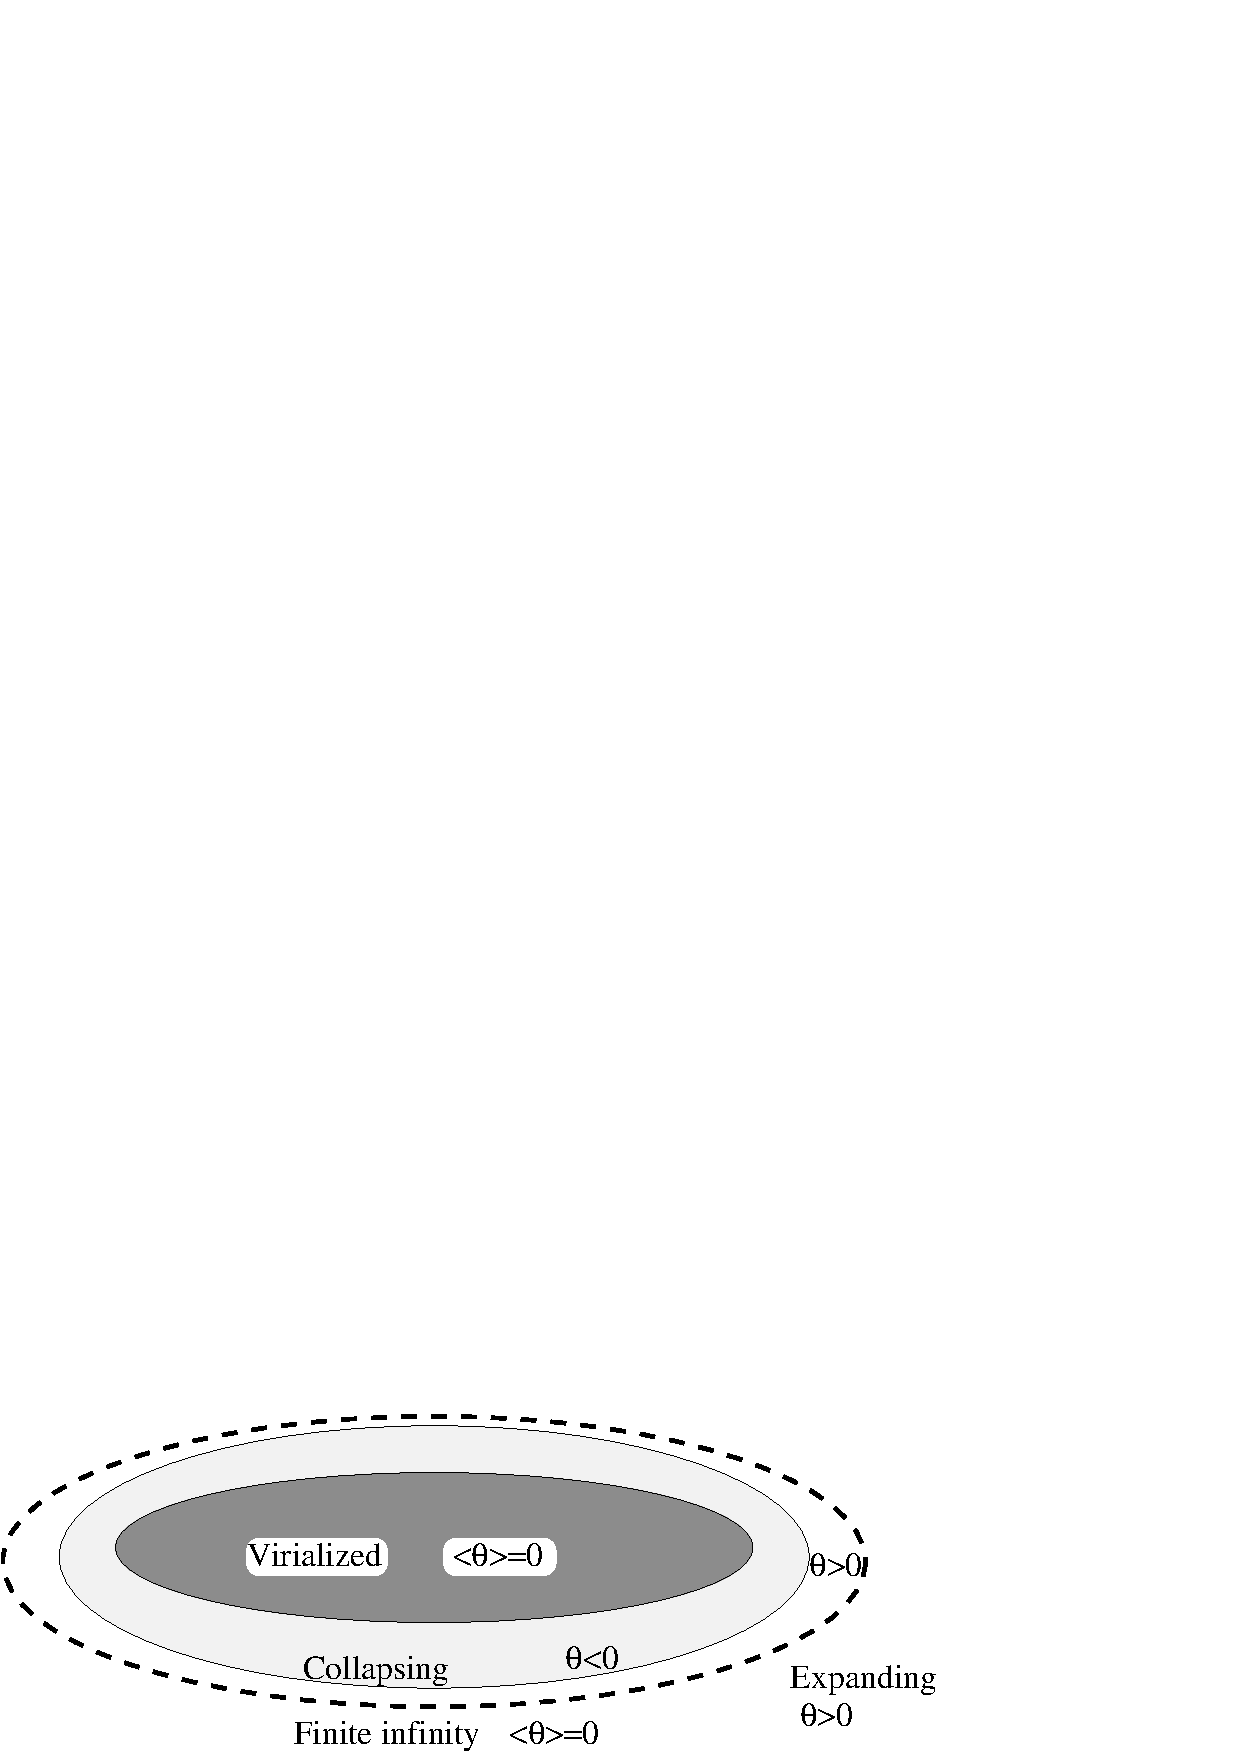
\includegraphics[height=\PartHeadHeight]{./images/part#1head\if@mainmatter\else\ifPaper\else-s\fi\fi}\@gobble}

%
% There are a couple of bits of classical Greek:
%   [Greek: hoi polloi]
%   [Greek: Kuklou metresis]
% We use the ibycus package if available, but if not we
% have a fallback to use math greek and fake the accents
\GenericInfo{*** }{***\MessageBreak
 Important Note: this document contains\MessageBreak
 a small amount of classical Greek; see comments in TeX source\@gobble}
\IfFileExists{psibycus.sty}
{% use ibycus greek with Type 1 fonts
 \GenericInfo{*** }{*** Attempting to use ibycus polytonic Greek\MessageBreak\expandafter\@gobble\@gobble}
 \usepackage{psibycus}[2004/10/18]
 \def\hoipolloi{{\greek{oi( polloi'}}}
 \def\Kukloumetresis{{\greek{Ku'klou me'trhsis}}}
}{% else fake with math greek
 \def\RoughBreathing{\mathaccent"012C }
 \def\hoipolloi{$o\RoughBreathing{\vphantom{(}\iota}$
    $\pi{o}\lambda\lambda{o}\acute\iota$}
 \def\Kukloumetresis{$K\!\acute\upsilon\kappa\lambda{o}\upsilon$
    $\mu\acute\epsilon\tau\!\rho\eta\sigma\iota\varsigma$}
 \GenericInfo{*** }{*** Faking breathed Greek using math\MessageBreak\expandafter\@gobble\@gobble}
}

\usepackage[utf8]{inputenc}[2004/02/05]  %changed latin1 to utf8
% \DeclareInputText{176}{\ensuremath{{^\circ}}} % suppress warnings about \textdegree in math
\DeclareUnicodeCharacter{00E3}{\^a} % added ã
\DeclareUnicodeCharacter{00EA}{\^e} % added ê

% mathematics
\usepackage[reqno]{amsmath}[2000/07/18]
\usepackage[psamsfonts]{amssymb}[2002/01/22]
% we only want inline equations to break where we explicitly allow
\binoppenalty=\@M
\relpenalty=\@M
\def\dotsc{\allowbreak\ldots}
\let\dotm\cdot
\let\epsilon\varepsilon
\let\phi\varphi
\def\Therefore{\therefore\;}
\DeclareMathOperator{\cosec}{cosec}
\def\maketag@@@#1{\hbox to2cm{\m@th\normalfont\dotfill#1}}
\def\tagform@#1{\maketag@@@{(\ignorespaces#1\unskip\@@italiccorr),}}
\def\Tagform@#1{\maketag@@@{(\ignorespaces#1\unskip\@@italiccorr).}}
\def\Tag{\let\tagform@\Tagform@\tag}
% for aligned equations with commentary
% should be replaced with amsmath equivalent if I can find one!
% left text & LHS & RHS & right text \cr
\newskip\@Centering \@Centering=0pt plus 1000pt minus 1000pt
\newenvironment{LRalign}{\[\let\\\cr\LR@lign}{\]\aftergroup\ignorespaces}
\def\LR@lign#1\end{\displ@y \tabskip=\displaywidth
  \halign to\displaywidth{\kern-\displaywidth
  \rlap{\@lign##}\tabskip=\@Centering
  &\hfil$\@lign\displaystyle{##}$\tabskip=\z@
  &$\@lign\displaystyle{{}##}$\hfil\tabskip=\@Centering
  &\llap{\@lign##}\tabskip=\z@\crcr
  #1\crcr}\end}

% to avoid over/underfull boxes without using explicit linebreaks
% when a paragraph contains lots of difficult-to-hyphenate stuff
\def\stretchyspace{\spaceskip0.5em plus 0.5em minus 0.25em}

% footnotes
\setlength{\footmarksep}{\z@}
\setlength{\footmarkwidth}{1.3em}
\newfootnoteseries{T} % for transcriber's notes
\renewcommand{\m@make@footnotetext}[1]{% fixing buglet in recent versions of memoir
  \@namelongdef{@footnotetext#1}##1{%
  \insert\@nameuse{footins#1}{%
%  \def\baselinestretch{\m@m@singlespace}%
  \reset@font\@nameuse{foottextfont#1}%
  \@preamfntext
  \hsize\columnwidth
  \protected@edef\@currentlabel{%
    \csname p@footnote#1\endcsname\@nameuse{@thefnmark#1}%
  }%
  \color@begingroup
    \@nameuse{@makefntext#1}{%
      \rule\z@\footnotesep{\@nameuse{foottextfont#1}\ignorespaces ##1}% bug was here
      \@finalstrut\strutbox}%
  \color@endgroup}\m@mmf@prepare}}
\plainfootstyle{T} % default
\renewcommand{\thefootnote}{\BringhurstX{footnote}}
\footmarkstyle{#1\hfill}
\footmarkstyleT{#1.\hfill}
\renewcommand{\foottextfont}{\footnotesize\normalfont}
\let\foottextfontT\foottextfont
\usepackage{perpage}[2002/12/20]
\MakePerPage{footnote}
\MakePerPage{footnoteT}
\newif\ifEditorials
% there are two kinds of transcriber's notes:
% those to do with the text (typos etc), and "editorial"
% comments/elaborations
% PG requires \Editorialsfalse, but if you're not a purist
% change to \Editorialstrue
\Editorialsfalse
\ifEditorials
  \let\Editorial\footnoteT\GenericInfo{\@spaces\@spaces\@spaces
    }{NB: Including transcriber's editorialisations}
\else
  \let\Editorial\@gobble\GenericInfo{\@spaces\@spaces\@spaces
    }{NB: Suppressing transcriber's editorialisations}
\fi
\def\BringhurstX#1{\expandafter\@BringhurstX\csname c@#1\endcsname}
\def\@BringhurstX#1{\ifcase#1\or*\or\dag\or\ddag\or\S\or$\|$\or\P
  \or**\or\dag\dag\or\ddag\ddag\or\S\S\or$\|\|$\or\P\P\else?\fi}
% Sometimes the author has multiple references on a page to the same footnote
% so we have to go to some lengths to discover if there's an intervening
% pagebreak or not since our pagination is unlikely to match the original.
% If there's a pagebreak we need a second copy of the footnote,
% but if not we need to duplicate the footnotemark.
% We need to insert labels for both footnotemark locations;
% the label names are passed as #1 and #2
% Syntax is \multifootnote{label 1}{label 2}{footnote text}
% Not sure if this is totally stable...
% Perhaps we could do this by accessing the perpage
% machinery somehow?
\def\multifootnote#1#2{%
  \expandafter\ifx\csname r@#1\endcsname\relax
   % labels undefined: don't do anything fancy this time
   \let\next\footnote
  \else
   \@tempcnta\expandafter\expandafter\expandafter
     \@secondoffive\csname r@#1\endcsname\relax
   \@tempcntb\expandafter\expandafter\expandafter
     \@secondoffive\csname r@#2\endcsname\relax
   \ifnum\@tempcnta=\@tempcntb
    % footnotes are on same page; duplicate footnotemark
    \addtocounter{footnote}{-1}\footnotemark\let\next\@gobble
   \else
    % pagebreak intervenes; duplicate entire footnote
    \let\next\footnote
   \fi\fi\next}
% The conventions regarding "ibidem" are that you can only use it
% when the citation is the same as that immediately preceding it
% *on the same spread*
% Since this may change with the pagination, we can't simply
% reproduce the author's original "ibid"s (unless they're inside
% a single footnote), but must check they are still on the
% same spread as what is being ibided
% #1 is case flag, #2 is label for other reference,
% #3 is alternative text for when ibid isn't allowed
\def\DP@ibid#1#2#3{\global\advance\c@vrcnt\tw@
  \label{ib@d:\the\c@vrcnt}\expandafter
  \ifx\csname r@#2\endcsname\relax
    % label not defined so no fancy stuff this time
    \csname #1bid\endcsname
  \else\expandafter
  \ifx\csname r@ib@d:\the\c@vrcnt\endcsname\relax
    % companion label not defined so avoid fancy stuff this time
    \csname #1bid\endcsname
  \else % check for matching spread
    \@tempcnta\expandafter\expandafter\expandafter
      \@secondoffive\csname r@#2\endcsname\relax
    \@tempcntb\expandafter\expandafter\expandafter
      \@secondoffive\csname r@ib@d:\the\c@vrcnt\endcsname\relax
    \ifnum\@tempcnta=\@tempcntb % same page: use ibid
      \csname #1bid\endcsname
    \else % not same page, so should have a < b
      \if@twoside % spreads make sense
        \ifodd\@tempcntb
          % should be on same spread, unless b=a+3 (highly unlikely)
          \csname #1bid\endcsname
        \else #3\fi
      \else #3\fi
    \fi
  \fi\fi}
\def\ibidref{\DP@ibid i}
\def\Ibidref{\DP@ibid I}
  % We want the footnotes to be out of the way at the bottom, but memoir
  %   sets \raggedbottom in screen mode, and in print mode there is sometimes
  %   insufficient stretch on a page.
\renewcommand*{\footnoterule}{\kern-3\p@\ifPaper\vglue0\p@ plus6\p@\else\vfill\fi
    \hrule width 0.4\columnwidth \kern 2.6\p@}

% We set up the version of the verbatim package embedded
% in the memoir class to wrap nicely
\setlength{\verbatimindent}{.25in}
\wrappingon
\addto@hook\afterevery@verbatim{\parindent\z@\relax}
\setverbatimfont{\normalfont\ttfamily\ifPaper\tiny\else\Small\fi} % 8pt for B5, 11pt for screen
\addto@hook\every@verbatim{\PGhook}
\let\verbatimbreakchar\empty
\let\PGhook\empty
{\catcode`\L\active
\gdef\PGlicencelink{\catcode`\L\active\letL\PGlinklicence}}
\def\PGlinklicence{\@ifnextchar i{\PG@lli}{L}}
\def\PG@lli#1{\@ifnextchar c{\PG@llii}{Li}}
\def\PG@llii#1{\@ifnextchar e{\PG@lliii}{Lic}}
\def\PG@lliii#1{\@ifnextchar n{\PG@lliv}{Lice}}
\def\PG@lliv#1{\@ifnextchar s{\PG@llv}{Licen}}
\def\PG@llv#1{\@ifnextchar e{\PG@llvi}{Licens}}
\def\PG@llvi#1{\hyperlink{PGlicence}{License}}
\def\PGheaderhook{\catcode`\L\active}

% half-title, title and copyright pages
\aliaspagestyle{title}{empty}
\setlength{\droptitle}{-2em}
\pretitle{\begin{center}\bfseries\ifPaper\LARGE
  \else\fontsize{30}{36}\selectfont\fi}
\renewcommand{\maketitlehookb}{\vspace{\z@\@plus.5fill}%\ifPaper\vspace{24pt}\else\medskip\fi
  \begin{center}\tiny\bfseries BY\end{center}}
\posttitle{\par\end{center}}
\preauthor{\begin{center}\Large}
\postauthor{\par\end{center}}
\def\affiliation#1{\def\theAffiliation{#1}}
\def\Edition#1{\def\theEdition{#1}}
\def\Publisher#1{\def\thePublisher{#1}}
\renewcommand{\maketitlehookc}{\begin{center}\tiny
  \textsc{\theAffiliation}\par\end{center}}
\predate{\vspace{\z@\@plus.5fill}\begin{center}\Small\textit{\theEdition}\end{center}
  \vspace{\z@\@plus.5fill}\begin{center}\large\textsc{\thePublisher}\par\normalsize\oldstylenums}
\postdate{\par\bigskip\SMALL[\textit{\theRights}]\end{center}\vspace{-1.5em}}
\def\Rights#1{\def\theRights{#1}}
\let\transcribersnotes\@empty
\let\transcribersNotes\@empty
\newcommand{\transcribersnote}[1]{%
  \@ifnotempty{#1}{\g@addto@macro\transcribersnotes{#1\par}%
    \@xp\@ifempty\@xp{\transcribersNotes}%
      {\renewcommand{\transcribersNotes}{note}}
      {\renewcommand{\transcribersNotes}{notes}}}}

\def\makecopyrightpage{% production credits and transcriber's notes
  \begingroup\pagestyle{empty}
  \ifPaper
    \null\vfil
    \transcribersnote{This document is designed for two-sided printing. Consequently, the
      many hyperlinked cross-references are not visually distinguished.
      The document can be recompiled for more comfortable on-screen viewing:
      see comments in source \LaTeX\ code. }
  \else
    \transcribersnote{This document is designed for on-screen viewing.
      It can be recompiled for two-sided printing: see comments in source \LaTeX\ code.
      Alternatively, print this on-screen version 2-up.}
  \fi
  \begin{center}
Produced by Joshua Hutchinson, David Starner, David Wilson
and the Online Distributed Proofreading Team at
http://www.pgdp.net
  \end{center}
  \vfil\vfil
  \vfil
  \vbox{\Small\hsize=.75\textwidth\parindent=\z@\parskip=.75em
  \textit{Transcriber's \transcribersNotes}\par\medskip\raggedright
  \transcribersnotes\par}
  \ifPaper\newpage\else\eject\fi\endgroup}

% parts, chapters and sections
% (for part i; we redefine sections for part ii later)
\usepackage{indentfirst}[1995/11/23]
\renewcommand{\printpartname}{\partnamefont\MakeUppercase{\partname}}
\renewcommand{\printpartnum}{\partnumfont \thepart.}
\renewcommand{\midpartskip}{\par\vskip3pc}
\renewcommand{\afterpartskip}{\vskip6pc\begin{adjustwidth}{5pc}{5pc}\small
  \itshape~\par\DP@PartQuote\end{adjustwidth}\global\let\DP@PartQuote\empty
  \vfil\newpage}
\newcommand{\PartQuote}[1]{\long\def\DP@PartQuote{#1}}
\let\DP@PartQuote\empty
\renewcommand{\parttitlefont}{\PartHeadHeight=\ifPaper17pt\else39pt\fi}
\makechapterstyle{rouseball}{%
  \ifPaper\setlength{\beforechapskip}{4pc}
    \else\setlength{\beforechapskip}{2pc}\fi
  \renewcommand{\chapnumfont}{\normalfont\huge\bfseries}
  \renewcommand{\printchapternum}{\chapnumfont\Roman{chapter}.}
  \renewcommand{\printchaptername}{\begin{center}\chapnumfont
    \MakeUppercase{\chaptername}}
  \renewcommand{\printchapternonum}{\begin{center}}
  \setlength{\midchapskip}{3pc}
  \renewcommand{\chaptitlefont}{\normalfont\Large\bfseries}
  \renewcommand{\printchaptertitle}[1]{\chaptitlefont\MakeUppercase{##1}}
  \setlength{\afterchapskip}{\@ne pc}
  \renewcommand{\afterchaptertitle}{\end{center}\nobreak\vskip\afterchapskip}
  }
\chapterstyle{rouseball}
\makechapterstyle{advert}{%
  \renewcommand{\printchapternum}{\chapnumfont\Roman{chapter}}
  \renewcommand{\printchaptername}{\begin{center}}
  \let\printchapternonum\printchaptername
  \setlength{\beforechapskip}{\z@}
  \setlength{\afterchapskip}{0.5em}
  \renewcommand{\chaptitlefont}{\normalfont\Large\bfseries}
  \renewcommand{\afterchaptertitle}{\end{center}\nobreak\vskip\afterchapskip}
  }
% kill section numbers so we can use unstarred versions to get bookmarks easily
\setsecnumformat{}
\setsecnumdepth{section} % we want bookmarks down to this level
\maxsecnumdepth{subsection}
\maxtocdepth{subsection}
\setlength{\parindent}{1.8em}
\setlength{\leftmargini}{1.8em}
\setsecheadstyle{\normalfont\normalsize\scshape}
\setsecindent{\parindent}
\setaftersecskip{-1.5em}
% because we are using run-in heads we need to force the paragraph to start
% otherwise the hyperlinks/contents page number can be on the previous page
% This means we can't have any blank lines between the \section and the
% beginning of the section text and we need to be careful about line endings
\def\@xsect #1{\@tempskipa #1\relax
  \ifdim \@tempskipa >\z@ \par \nobreak \vskip \@tempskipa \@afterheading
  \else \@nobreakfalse \global \@noskipsectrue \everypar {\if@noskipsec
    \global \@noskipsecfalse {\setbox \z@ \lastbox }\clubpenalty \@M
    \begingroup \@svsechd \endgroup \unskip \@tempskipa #1\relax
    \hskip -\@tempskipa \else \clubpenalty \@clubpenalty \everypar {}\fi
    }\leavevmode
  \fi \ignorespaces}
% we need this because the \phantomsection inserted by hyperref blocks the
% \ignorespaces at the end of section header processing
% and if we have a \phantomsection in vertical mode a page break
% can happen between the link and the "section's" text
\AtBeginDocument{\let\PGph@ntomsecti@n\phantomsection
  \def\phantomsection{\leavevmode\PGph@ntomsecti@n\ignorespaces}}
\setsubsecheadstyle{\normalfont\normalsize\itshape}
\setsubsecindent{\parindent}
\setbeforesubsecskip{\z@}
\setaftersubsecskip{-1em}
% section/subsection headings get an added period,
% because we don't want the period in the ToC
\def\Sectionformat#1#2{#1.}
\def\chapindex{\specialindex{\jobname}{chapter}}
\newcommand{\ssection}{% Like a section but without the preceding big skip
  \sechook%
  \@startsection{section}{1}%  level 1
      {\secindent}%            heading indent
      {-0.5ex \@plus -0.1ex \@minus -.2ex}%        skip before the heading
      {\aftersecskip}%         skip after the heading
      {\normalfont\secheadstyle}} % font
% In part ii the author uses slightly different heading styles
% so we set up switches for these here
% For Chapter VIII the section headings are italic
% and centered rather than small caps and run-in as in part i.
\def\UseChapterVIIIHeadings{%
 \setsecheadstyle{\normalfont\normalsize\centering\itshape}
 \setsecindent{0pt}
 \setaftersecskip{2.3ex plus.2ex}}
% For Chapter XIV we need to restore the section headings to the style used in part i
% although now subsections have a small space above
% and the sections etc are numbered
\def\UseChapterXIVHeadings{%
 \setsecheadstyle{\normalfont\normalsize\scshape}
 \setsecindent{\parindent}
 \setaftersecskip{-1.5em}
 \setbeforesubsecskip{-1ex plus -.2ex minus -.1ex}
 \defaultsecnum
 \renewcommand{\thesection}{\Roman{section}.}
 \renewcommand{\thesubsection}{{\upshape(\roman{subsection})}}}


% table of contents
\renewcommand{\contentsname}{TABLE OF CONTENTS.}
\setpnumwidth{2.75em}
\setrmarg{3.5em}
\setlength{\cftpartnumwidth}{\z@}
\renewcommand{\cftpartfillnum}[1]{\par}
\def\partnumberline#1#2.{\vbox{%
  \centerline{PART #1.}\ifPaper\kern4ex\else\kern2ex\fi
  \centerline{\PartHeadHeight=17pt#2.}\kern3ex\vfil}%
  \aftergroup\setpartlinkheight}
\def\setpartlinkheight{\baselineskip=\ifPaper5\else4\fi\baselineskip}
\setlength{\cftchapternumwidth}{\z@}
\renewcommand{\cftchapterfillnum}[1]{\par}
\renewcommand{\cftchapterfont}{\scshape}
\def\chapternumberline#1#2.{\vbox{%
  \centerline{\if!#1!\else Chapter \@Roman{#1}.\fi\qquad#2.}\par\kern2ex}%
  \aftergroup\setchaplinkheight}
\def\setchaplinkheight{\baselineskip=2.5\baselineskip}
\cftsetindents{section}{\z@}{2.3em}
\cftsetindents{subsection}{1.5em}{3.2em}
\let\numberline\@gobble % suppresses section etc numbers
% the following machinations are to (a) encourage pagebreaks in the ToC
% at chapter divisions, (b) to discourage separating subsections from their
% section, and (c) to write "PAGE" just above the first section entry on any
% page [NB if ToCPAGE has any vertical size the pagination frequently fails
% to stabilise; since it's always at the top of a page or just below a
% chapter line it can never overlap anything]
\newcount\DPtoc
\DPtoc\m@ne
\def\ToCPAGE{\hrule height\z@ depth\z@
     \setbox\z@=\vbox{\rightline{\SMALL PAGE}}\ht\z@=\z@\dp\z@=\z@\vskip-1ex
     \box\z@\vskip1ex}
\def\firstfilbreak{\let\secfilbreak\filbreak}
\AtBeginDocument{% so we don't get clobbered by hyperref
  \let\DPaddcontentsline\addcontentsline
  \def\addcontentsline#1#2#3{\hbox to\z@{\hss % this is because somewhere space is leaking so we neutralise it
    \expandafter\ifx\csname l@#2\endcsname\l@chapter
      \addtocontents{#1}{\protect\bigskip\protect\filbreak\protect\let
        \protect\secfilbreak\protect\firstfilbreak}%
      \DPaddcontentsline{#1}{#2}{#3}%
    \else\expandafter\ifx\csname l@#2\endcsname\l@subsection
      \addtocontents{#1}{\protect\nobreak}%
      \DPaddcontentsline{#1}{#2}{#3\protect\tocsecspacer}%
    \else\expandafter\ifx\csname l@#2\endcsname\l@section
      \addtocontents{#1}{\protect\edef\protect\DP@tmp{{\protect\expandafter
          \protect\ifx\protect\csname r@toc:subsec:\number\DPtoc
          \protect\endcsname\protect\relax??\protect\else
          \protect\expandafter\protect\expandafter\protect\expandafter
          \protect\@secondoffive\protect\csname r@toc:subsec:\number\DPtoc
          \protect\endcsname\protect\fi}}}%
      \global\advance\DPtoc\@ne\relax
      \addtocontents{#1}{\protect\edef\protect\DP@tmp{\protect\DP@tmp
          {\protect\expandafter\protect\ifx\protect
          \csname r@toc:subsec:\number\DPtoc\protect\endcsname\protect
          \relax??\protect\else\protect\expandafter\protect\expandafter
          \protect\expandafter\protect\@secondoffive\protect
          \csname r@toc:subsec:\number\DPtoc\protect\endcsname\protect\fi}}}%
      \addtocontents{#1}{\protect\expandafter\protect\nametest\protect\DP@tmp}%
      \addtocontents{#1}{\protect\secfilbreak\protect\ifsamename\protect\else
          \protect\ToCPAGE\protect\fi}%
      \DPaddcontentsline{#1}{#2}{#3\protect\tocsecspacer\protect
        \label{toc:subsec:\number\DPtoc}}%
    \else
      \DPaddcontentsline{#1}{#2}{#3}%
    \fi\fi\fi\hss}\ignorespaces}%
 }
\def\tocsecbox#1{\ifPaper\vbox{\leftskip\z@\expandafter\@tempdima\@pnumwidth
  \advance\hsize-\@tempdima\raggedright\hyphenpenalty=10000
  \emergencystretch.5\hsize
  \noindent\vrule height12pt width\z@ depth\z@ % to give the illusion of
% evenly-spaced lines, together with the vphantom inserted above
  \hangindent1.5em\hangafter1\parfillskip\z@#1\cftsectionleader\null
  \par}\aftergroup\settocsecboxlinkheight\else#1\fi}
\ifPaper\def\settocsecboxlinkheight{\baselineskip=2\baselineskip}\fi
\def\tocsecspacer{\vphantom{\normalfont Pp}}

% headers and footers
\copypagestyle{frontstuff}{headings}
  \makeevenhead{frontstuff}{\normalfont\SMALL\thepage}{\normalfont
    \SMALL\MakeUppercase{\leftmark}}{}
  \makeoddhead{frontstuff}{}{\normalfont\SMALL\MakeUppercase{\rightmark}}%
    {\normalfont\SMALL\thepage}
\makepsmarks{frontstuff}{%
      \let\@mkboth\markboth
      \def\chaptermark##1{%
        \markboth{\MakeUppercase{##1}}{\MakeUppercase{##1}}}%
      \def\tocmark{%
        \markboth{\MakeUppercase{\contentsname}}{\MakeUppercase{\contentsname}}}%
    }
\makeevenfoot{frontstuff}{}{\SMALL\wmc}{}
\makeoddfoot{frontstuff}{}{\SMALL\wmc}{}
\pagestyle{frontstuff}
\copypagestyle{part}{plain}
\copypagestyle{chapter}{plain}
\ifPaper
  % because we are using a 2-page spread format we make a bit of fuss about page-turning hyphenation
  % the large \brokenpenalty makes it hard to end the next (odd/recto) page with a hyphen
  \makeevenfoot{part}{}{\normalfont\SMALL\wmc\thepage}{\global\brokenpenalty10000}
  % the small \brokenpenalty makes it less hard to end the next (even/verso) page with a hyphen
  % (because the other end of the hyphen will still be visible on the same spread)
  \makeoddfoot{part}{}{\normalfont\SMALL\wmc\thepage}{\global\brokenpenalty150}
  \makeevenfoot{chapter}{}{\normalfont\SMALL\wmc\thepage}{\global\brokenpenalty10000}
  \makeoddfoot{chapter}{}{\normalfont\SMALL\wmc\thepage}{\global\brokenpenalty150}
\else
  \makeevenfoot{part}{}{\normalfont\SMALL\wmc\thepage}{}
  \makeoddfoot{part}{}{\normalfont\SMALL\wmc\thepage}{}
  \makeevenfoot{chapter}{}{\normalfont\SMALL\wmc\thepage}{}
  \makeoddfoot{chapter}{}{\normalfont\SMALL\wmc\thepage}{}
\fi
\copypagestyle{mainstuff}{headings}
\makepsmarks{mainstuff}{%
      \let\@mkboth\markboth
      \def\chaptermark##1{%
        \markboth{\MakeUppercase{##1}}{\MakeUppercase{##1}}}%
      \def\sectionmark##1{%
        \markright{\MakeUppercase{##1}.}}% note the added period
      \let\subsectionmark\sectionmark
      \def\indexmark{\markboth{\MakeUppercase{\indexname}.}%
        {\MakeUppercase{\indexname}.}}%
    }
\def\mainstuffChapNumOdd{CH. \Roman{chapter}]}
\def\mainstuffChapNumEven{[CH. \Roman{chapter}}
\ifPaper
  \makeevenhead{mainstuff}{\normalfont\SMALL\thepage}{\normalfont
    \SMALL\MakeUppercase{\leftmark}}{\normalfont\SMALL\mainstuffChapNumEven}
  \makeoddhead{mainstuff}{\normalfont\SMALL\mainstuffChapNumOdd}{\normalfont
    \SMALL\MakeUppercase{\rightmark}}{\normalfont\SMALL\thepage}
  \makeevenfoot{mainstuff}{}{\SMALL\wmc}{\global\brokenpenalty10000}
  \makeoddfoot{mainstuff}{}{\SMALL\wmc}{\global\brokenpenalty150}
\else
  \makeoddhead{mainstuff}{\normalfont\SMALL\mainstuffChapNumOdd}{\normalfont
    \SMALL\MakeUppercase{\ifodd\count\z@\rightmark\else\leftmark
    \fi}}{\normalfont\SMALL\thepage}
  \makeoddfoot{mainstuff}{}{\SMALL\wmc}{}

\fi

% make cross-page hyphenation difficult by default
\brokenpenalty10000

\copypagestyle{adverts}{headings}
\makeevenhead{adverts}{\normalfont\SMALL\thepage}{}{}
\makeoddhead{adverts}{}{}{\normalfont\SMALL\thepage}
\makeevenfoot{adverts}{}{\SMALL\wmc}{}
\makeoddfoot{adverts}{}{\SMALL\wmc}{}
\copypagestyle{licence}{headings}
\makeevenhead
  {licence}{\normalfont\SMALL\thepage}{\normalfont\SMALL LICENSING.}{}
\makeoddhead
  {licence}{}{\normalfont\SMALL LICENSING.}{\normalfont\SMALL\thepage}
\makeevenfoot{licence}{}{\SMALL\wmc}{}
\makeoddfoot{licence}{}{\SMALL\wmc}{}

% for quotations, which in this book were printed full-width in a smaller
% font but we will use small font *and* slightly narrower text block
\AtBeginDocument{\let\QuoteFont\Small}
\newenvironment{Quotation}{\QuoteFont\partopsep\z@\quotation}{\par\medskip
  \global\advance\@listdepth\m@ne}
% for exam questions in Chapter vii: smaller font but full-width
\newenvironment{ExamQuestions}{\QuoteFont\medskip\def\Q[##1]{\par\indent
  \hbox to\parindent{##1\hss}\ignorespaces}}{\medskip}

% illustrations
% (external files are provided as both .eps and .pdf;
% a few are bitmaps lifted from page scans, most from hand-coded PostScript)
\usepackage{flafter}[2000/07/23]
\ifPaper % defaults are not stretchy enough
 \setlength\textfloatsep{20\p@ \@plus 6\p@ \@minus 4\p@}
 \setlength\intextsep   {14\p@ \@plus 8\p@ \@minus 4\p@}
\fi
% driver should be specified in graphics.cfg;
% if not, add explicit option to graphicx call
\usepackage[final]{graphicx}[1999/02/16]
\GenericWarning{*** }{***\MessageBreak
 Important Note: this document comes with a full set of\MessageBreak
 graphics in EPS (Encapsulated PostScript, not MetaPost) format\MessageBreak
 and an equivalent full set compiled as PDF. If your workflow\MessageBreak
 requires another conversion make sure you know what you're doing!\MessageBreak\expandafter\@gobble\@gobble}
% we limit file extensions because different TeX systems search in different orders
% and the default ordering of extensions may lead to the wrong file being located
\ifpdf\DeclareGraphicsExtensions{.pdf}\else\DeclareGraphicsExtensions{.eps}\fi

% to refer to an uncaptioned illustration depending on
% where LaTeX has actually floated it to
% although it doesn't help with deciding above/below on
% a particular page
\usepackage{varioref}[2004/02/27]
% add hook to enable uppercasing first character
\newif\ifVariorefUC
\VariorefUCfalse
\def\Vpageref{\VariorefUCtrue\vpageref}
\def\Varioif#1#2{\ifVariorefUC#1\else#2\fi\VariorefUCfalse}
% add links to references which don't call \pageref
\def\reftextfaceafter {\Varioif Oon the \Acrobatmenu
  {NextPage}{\reftextvario{facing}{next} page}}
\def\reftextfacebefore{\Varioif Oon the \Acrobatmenu
  {PrevPage}{\reftextvario{facing}{preceding} page}}
\def\reftextafter {\Varioif Oon the \Acrobatmenu
  {NextPage}{\reftextvario{following}{next} page}}
\def\reftextbefore {\Varioif Oon the \Acrobatmenu
  {PrevPage}{\reftextvario{preceding}{previous} page}}
\def\reftextcurrent{\Varioif Oon \reftextvario{this}{the current} page}
\def\reftextfaraway#1{\Varioif Oon page~\pageref{#1}}
\def\reftextpagerange#1#2{\Varioif Oon pages~\pageref{#1}--\pageref{#2}}
% suppress a link if it goes to the same page
% requires destination to have been created by \DPlabel
\def\vhyperlink{\begingroup\@ifstar
  {\vhyperl@nkstar}{\vhyperl@nk}}
\def\vhyperl@nkstar#1#2{%
  \def\reftextfaceafter{\unskip#2}\let\reftextfacebefore\reftextfaceafter
  \def\reftextafter{\hyperlink{#1}{#2}}\let\reftextbefore\reftextafter
  \let\reftextcurrent\reftextfaceafter
  \def\reftextfaraway##1{\hyperlink{#1}{#2}}\let\vref@space\relax
  \vp@geref{#1}{}\endgroup}
\def\vhyperl@nk#1#2{%
  \def\reftextfaceafter{#2}\let\reftextfacebefore\reftextfaceafter
  \def\reftextafter{\hyperlink{#1}{#2}}\let\reftextbefore\reftextafter
  \let\reftextcurrent\reftextfaceafter
  \def\reftextfaraway##1{\hyperlink{#1}{#2}}\let\vref@space\space
  \vp@geref{#1}{}\endgroup}
% captions look like \textit{Figure} \lowercaseroman{n}.
% but since they aren't always numbered consecutively we use
% \legend (with hard-coded numbers if necessary) rather than \caption
\captionstyle{\centering}
\captiontitlefont{\normalfont\Small\itshape}
\def\Uproman#1{\upshape\@roman{#1}.}
% For magic squares we use a picture environment rather than tabular/array
% We first redefine the horizontal/vertical lines for the picture environment
% to give them squarecap ends a la PostScript: this makes the corners of
% frames join up neatly
\def\@hline{\advance\@linelen\@wholewidth
  \ifnum \@xarg <\z@ \hskip -\@linelen \hskip\@halfwidth
    \else\hskip-\@halfwidth\fi
  \vrule \@height \@halfwidth \@depth \@halfwidth \@width \@linelen
  \ifnum \@xarg <\z@ \hskip -\@linelen \hskip\@halfwidth
    \else\hskip-\@halfwidth\fi}
\def\@upline{%
  \hb@xt@\z@{\advance\@linelen\@halfwidth\hskip -\@halfwidth
   \vrule \@width \@wholewidth \@height \@linelen \@depth \@halfwidth\hss}}
\def\@downline{%
  \hb@xt@\z@{\advance\@linelen\@halfwidth\hskip -\@halfwidth
   \vrule \@width \@wholewidth \@height \@halfwidth \@depth \@linelen \hss}}
% Now we set up a MagicSquare environment, which is a bit like a tabular
% except that the entries must be enclosed in braces if they have > 1 digit
% \begin{MagicSquare}{horiz order}[optional vertical order, defaults to square]
%   {entry} & {entry} & ... & {entry}\\
% \end{MagicSquare}
\def\Sq@r#1{\vbox to\SqHt{\vss\hbox to\SqWd{\smaller\hss$\vphantom
  {\SqHtDefault}#1$\hss}\vss}}
\def\SqHtDefault{1}
\def\Cell(#1,#2;#3){\put(#1,#2){\framebox{\Sq@r{#3}}}}
\def\MagicSquare#1{\catcode`\&=\active
  \@ifnextchar[{\M@gicSqu@re#1}{\M@gicSqu@re#1[#1]}}
\long\def\M@gicSqu@re#1[#2]#3\end{%
  \let\\\MSqN@xtC@ll
  \begin{picture}(#1,#2)
   \@tempcnta=#2
   \MSqN@xtC@ll#3
   \put(0,0){\line(0,1){#2}}
   \put(0,0){\line(1,0){#1}}
   \put(#1,0){\line(0,1){#2}}
   \put(0,#2){\line(1,0){#1}}
  \end{picture}\end}
\let\endMagicSquare\empty
\let\MSqHorizAdvance\@ne
\let\MSqVertAdvance\m@ne
\long\def\MSqN@xtCell#1{\advance\@tempcntb\MSqHorizAdvance
  \Cell(\@tempcntb,\@tempcnta;#1)}
\long\def\MSqN@xtC@ll{\ifnum\@tempcnta=\z@\let\next\relax\else
  \advance\@tempcnta\MSqVertAdvance\@tempcntb=-\MSqHorizAdvance
  \let\next\MSqN@xtCell\fi\next}
{\catcode`\&=\active
\global\let&=\MSqN@xtCell}
\unitlength=1.5em
\linethickness{0.14em}
\fboxsep\z@
\def\SqHt{1.5em}
\def\SqWd{1.5em}
\RequirePackage{wrapfig}[2003/01/31]
% for the diagrams explaining Chinese rings
\def\RingDiagram#1#2#3#4#5#6#7{%
\begin{picture}(42,8)
\put(0,0){\line(0,1){8}}
\put(0,4){\line(1,0){42}}
\put(4,\ifcase#1 1\or7\fi){\circle{3}}
\put(10,\ifcase#2 1\or7\fi){\circle{3}}
\put(16,\ifcase#3 1\or7\fi){\circle{3}}
\put(22,\ifcase#4 1\or7\fi){\circle{3}}
\put(28,\ifcase#5 1\or7\fi){\circle{3}}
\put(34,\ifcase#6 1\or7\fi){\circle{3}}
\put(40,\ifcase#7 1\or7\fi){\circle{3}}
\end{picture}\\}
\def\RingDiag#1#2#3#4#5{%
\begin{picture}(42,10)
\put(0,0){\line(0,1){8}}
\put(0,4){\line(1,0){42}}
\put(4,\ifcase#1 1\or7\fi){\circle{3}}
\put(13,\ifcase#2 1\or7\fi){\circle{3}}
\put(22,\ifcase#3 1\or7\fi){\circle{3}}
\put(31,\ifcase#4 1\or7\fi){\circle{3}}
\put(40,\ifcase#5 1\or7\fi){\circle{3}}
\end{picture}}
% note the multirow package does not supply a date in \ProvidesFile format
% we used multirow.sty  V1.6 version (5-May-2004)
\usepackage{multirow}

% to deal with the scanned page breaks
% add a "draft" option to the documentclass invocation
% to see the scan numbers
\ifdraftdoc
\def\PG#1 #2.png#3
{\marginpar{\noindent\null\hfill\Small #2.png}}
\def\PGx#1 #2.png#3
{}
\ifPaper\else\advance\marginparwidth15pt\fi
\else
\def\PG#1 #2.png#3
{}
\let\PGx\PG
\fi

% for thought breaks
% if it won't fit on the page, we squeeze in a rule instead
\newcommand\ThoughtBreakDP{\noindent
  \hbox to\textwidth{\hglue\z@\@plus\@ne fil*\hglue\z@\@plus0.2fil*\hglue\z@
    \@plus0.2fil*\hglue\z@\@plus0.2fil*\hglue\z@\@plus0.2fil*\hglue\z@
    \@plus\@ne fil}}
\newcommand\ThoughtBreakRule{\hbox to\textwidth{\hfil
  \vrule height\z@ depth.4pt width.3\textwidth\relax\hfil}}
\let\Th@ughtBre@k\ThoughtBreakRule
\newcommand\ThoughtBreakSpace{\vskip1.5em plus .5em\relax}
\newcommand\ThoughtBreak{\par\hrule height\z@ depth\z@
  \nobreak\begingroup
  \setbox\@tempboxa=\vbox{\ThoughtBreakSpace\Th@ughtBre@k}%
  \dimen@\pagegoal\advance\dimen@-\pagetotal % space left on page
  \ifdim\ht\@tempboxa>\dimen@ % not enough space left
    \ifdim\dimen@>\z@ % but there is some space to fill
      \vskip-\pagedepth\@plus\@ne fil
    \fi
    \setbox\@tempboxa=\vbox{\ThoughtBreakRule}% without any space before
    \ht\@tempboxa\z@\dp\@tempboxa\z@\box\@tempboxa
    \break
  \else % the normal thought break should fit
    \box\@tempboxa
    \ThoughtBreakSpace
  \fi\endgroup}

% PDF stuff: links, document info, etc
% Originally coded with a PostScript workflow in mind;
% if default driver given in hyperref.cfg is not suitable,
% add appropriate explicit option to hyperref call
\usepackage[final,colorlinks]{hyperref}[2003/11/30]
% we check if the driver is the useless (for pdf) "hypertex",
% and if so we force dvips instead and issue a warning
\usepackage{memhfixc}[2004/05/13]
\providecommand{\ebook}{2xydw} % real ebook number supplied during WW
\hypersetup{pdftitle=The Project Gutenberg eBook \#\ebook: Mathematical Recreations and Essays,
  pdfsubject=Mathematical Recreations and Essays,
  pdfauthor=W. W. Rouse Ball,
  pdfkeywords={David Starner, Joshua Hutchinson, David Wilson,
               Project Gutenberg Online Distributed Proofreading Team},
  pdfstartview=Fit,
  pdfstartpage=1,
  pdfpagemode=UseNone,
  pdfdisplaydoctitle,
  bookmarksopen,
  bookmarksopenlevel=1,
  linktocpage=false}
\ifPaper
  \hypersetup{pdfpagescrop=0 0 499 709, b5paper, % b5 176x250mm
     pdfpagelayout=TwoPageRight,
     plainpages=false, linkcolor=\ifdraftdoc blue\else black\fi,
     menucolor=\ifdraftdoc blue\else black\fi,
     urlcolor=\ifdraftdoc magenta\else black\fi}
\else
  \hypersetup{pdfpagescrop=0 0 648 432, % ebook 9x6"
     pdfpagelayout=SinglePage, linkcolor=blue, menucolor=blue,
     urlcolor=magenta}
  \ifpdf\else % here we assume dvips or dvipsone is being used
    \AtBeginDocument{\special{! <</PageSize [648 432]>> setpagedevice}}
  \fi
\fi
% pdf annotations
\ifpdf % using native pdftex
   \def\wm{\noindent\kern.5\textwidth\pdfannot width\textwidth height12pt {\wmGuts}}
   \def\gext{pdf}
\else\expandafter\ifx\csname pdfmark\endcsname\relax\else % pdfmarks: we're using dvips or dvipsone
   \def\wm{\kern-12pt\noindent\kern.5\textwidth\rlap{\pdfmark[\phantom{\vrule width\textwidth
      height12pt}]{pdfmark=/ANN, Raw={\wmGuts}}}}
   \def\gext{eps}
\fi\fi
\def\wmGuts{/Subtype /FreeText
     /Contents (\string\200 Project \string\200 Gutenberg \string\200 \#\ebook\ \string\200)
     /DA ([0.6875 0.6875 0.6875] r
     /CoBo 8 Tf) /BS << /W 0 >> /F 37 /Q 1 /Title (PG)
     /DS(font: bold Courier,monospace 8.0pt;
         text-align:\ifPaper center\else right\fi; color:####BBBBBB )}
\newbox\wmbox
\def\wmc{\copy\wmbox}
\AtBeginDocument{\setbox\wmbox=\hbox to\z@{\hss
  \vtop{\hsize=\textwidth\kern\ifPaper35\else20\fi pt\wm}\hss}
  \ht\wmbox=\z@\relax\dp\wmbox=\z@\relax}
% slight modification of hyperref's command,
% for adding explicit bookmarks and destinations
\newcommand\DPpdfbookmark[3][0]{\rlap{\hyper@anchorstart{#3}\hyper@anchorend
     \Hy@writebookmark{}{#2}{#3}{#1}{toc}}}
\newcommand\DPlabel[1]{\rlap{\hyper@anchorstart{#1}\hyper@anchorend}\label{#1}}
% hyperref seems to use the most recent section anchor instead of page
% anchors in a \pageref, so we have to fix that; using AtBeginDocument
% so hyperref doesn't clobber it
\AtBeginDocument{\def\pageref#1{%
  \expandafter\@pagesetref\csname r@#1\endcsname\@empty{#1}}}

% bits and pieces
\emergencystretch=12pt
\let\Small\footnotesize
\let\SMALL\scriptsize
% We wanted to \usepackage{relsize} but the new version
% doesn't behave the same as the old version (which is what we wanted)
% so we just include the relevant bits from the old package
% written by Donald Arseneau
\DeclareRobustCommand\relsize[1]{%
\ifmmode \@nomath\relsize\else
 \@tempcnta % assign number representing current font size
   \ifx\@currsize\normalsize 4\else   % funny order is to have most ...
    \ifx\@currsize\small 3\else       % ...likely sizes checked first
     \ifx\@currsize\footnotesize 2\else
      \ifx\@currsize\large 5\else
       \ifx\@currsize\Large 6\else
        \ifx\@currsize\LARGE 7\else
         \ifx\@currsize\scriptsize 1\else
          \ifx\@currsize\tiny 0\else
           \ifx\@currsize\huge 8\else
            \ifx\@currsize\Huge 9\else
            4\rs@unknown@warning % unknown state: \normalsize as starting point
 \fi\fi\fi\fi\fi\fi\fi\fi\fi\fi
%  Change the number by the given increment:
 \advance\@tempcnta#1\relax
%  watch out for size underflow:
 \ifnum\@tempcnta<\z@ \rs@size@warning{small}{\string\tiny}\@tempcnta\z@ \fi
 \ifcase\@tempcnta  % set new size based on altered number
    \tiny \or \scriptsize \or \footnotesize \or \small \or \normalsize \or
    \large \or \Large \or \LARGE \or \huge \or \Huge \else
     \rs@size@warning{large}{\string\Huge}\Huge
\fi\fi}
\DeclareRobustCommand\larger[1][\@ne]{\relsize{+#1}}
\DeclareRobustCommand\smaller[1][\@ne]{\relsize{-#1}}
\DeclareRobustCommand\textlarger[2][\@ne]{{\relsize{+#1}#2}}
\DeclareRobustCommand\textsmaller[2][\@ne]{{\relsize{-#1}#2}}
\newcommand\mathsmaller[1]{{\mathchoice{\textstyle}%
  {\scriptstyle}{\scriptscriptstyle}{\scriptscriptstyle}#1}}
\DeclareRobustCommand\mathlarger[1]{\mathchoice
  {\mbox{\larger$\displaystyle#1\m@th$}}%
  {{\displaystyle#1}}{{\textstyle#1}}{{\scriptstyle#1}}}
%
\usepackage{longtable}[2004/02/01]
\usepackage{afterpage}[1995/10/27]
% for the dittos in one of the longtables
\def\Ditto#1#2#3{\expandafter
  \ifx\csname r@LT:row:#1\endcsname\relax % labels not defined, use "
  "\else
  \@tempcnta\expandafter\expandafter\expandafter
    \@secondoffive\csname r@LT:row:#1\endcsname\relax
  \@tempcntb\expandafter\expandafter\expandafter
    \@secondoffive\csname r@LT:row:#2\endcsname\relax
  \ifnum\@tempcnta<\@tempcntb #3\else "\fi\fi}
% for dots in an alignment
\def\dotfillatleast#1{%
  \leavevmode
  \@tempcnta=#1\@tempdima=\z@
  \loop\ifnum\@tempcnta>0%
    \advance\@tempdima by.44em\advance\@tempcnta\m@ne\repeat
  \leaders \hb@xt@ .44em{\hss.\hss}\expandafter\hskip\@tempdima plus1fill
  \kern\z@
}
% for really long "words" in the cryptography chapter
\def\CryptoSetup{\def\.{\hglue0ptplus.05pt\discretionary{}{}{}}}
% for descriptions of configurations within the colour cube section
% to ensure any linebreak keeps at least two parameters together
\def\Cube(#1; #2; #3, #4, #5, #6){($#1$;~$#2$; $#3$,~$#4$, $#5$,~$#6$)}
% common abbreviations (can be modified if desired)
\def\IE{\textit{i.e.}}
\def\Eg{\textit{ex.~gr.}}
\def\EG{\textit{Ex.~gr.}}
\def\eg{\textit{e.g.}}
\def\ibid{\textit{ibid.}}
\def\Ibid{\textit{Ibid.}}
\def\etseq{\textit{et seq.}}
\def\sic{\textit{sic}}
% The standard summation symbol seems too overwhelming when used inline,
% especially without limits
% We could use \Sigma, but it is subtly different from \sum, hence...
\def\textsum{\raise.4ex\hbox{$\m@th\mathsmaller{\sum}$}}

% a spacing kludge for one array
\def\DParraykludge{\setbox0=\copy\@arstrutbox\@tempdima=\ht0
 \advance\@tempdima by3pt\ht0=\@tempdima\box0 }

% details for printing out the index
%
% Important note: because of the way memoir double-handles certain commands,
% whenever there's (for example) \textit{foo} inside an \index inside a footnote,
% it ends up in the .idx as "\textit  {foo}" and if there are other \index commands
% (not in footnotes) for the same index entry, then these need to write the \textit
% explicitly with the two spaces, whereas inside the footnote it should be \textit{foo}
% with no spaces. Otherwise the \index commands from inside the footnotes won't get
% included with those from outside, and there will be two sets of entries in the index.
% This is important when maintining this file, because the apparently extraneous double
% spaces in various \index commands are intentional. See for example the various index
% entries for Bachet's Problèmes, Oughtred's Recreations and Ozanam's Recreations.
\noindexintoc
% to get balanced columns without doing it manually


\usepackage{multicol}[2006/05/18]
\onecolindextrue
\def\preindexhook{\phantomsection
  \addtocontents{toc}{\protect\bigskip}
  \addtocontents{toc}{\protect\let\protect\l@chapter\protect\l@section}
  \DPaddcontentsline{toc}{chapter}{\protect\textsc{\indexname}}
  \setlength{\columnseprule}{\z@}%
  \setlength{\columnsep}{\indexcolsep}%
  \multicols{2}\def\endtheindex
    {\def\@currenvir{multicols}\endmulticols}}
\def\hyperspindexpage(#1)#2{\hyperlink{page.#1}{chap. \textsc{\@roman{#2}}}}
\def\PrintTheIndex{\begingroup
\small
% although the original starts the index recto (p379) there's no reason
% to suppose this is essential (p378 is not blank) since some chapters
% start verso in the original
\clearpage
\let\mainstuffChapNumOdd\empty
\let\mainstuffChapNumEven\empty
\setlength\indexcolsep{15pt}
\ifPaper
  \renewcommand{\indexspace}{\par\penalty-3000 \vskip 10pt plus5pt minus3pt\relax}
\else
  \renewcommand{\indexspace}{\par\penalty-3000 \vskip 12pt plus6pt minus4pt\relax}
\fi
\raggedright\hyphenpenalty=10000\emergencystretch.5\hsize
\printindex
\endgroup}
\def\Printer#1{\vspace*{\z@\@plus1fill}{\centering
  \miniscule\hrule\smallskip#1\par}\eject}

% hyphenation hints
\hyphenation{Win-ches-ter se-cond theo-ry}

% avoid really short final lines of paragraphs if possible
\parfillskip=\z@\@plus0.85\textwidth

% hard-code various document dimensions to try to minimise
% effects of changes to class/package defaults
% (these values mostly based on mempatch 4.9a)
%
% tiny amount of stretch in the parskip improves appearance of slightly-short pages
\parskip\z@\@plus\p@\relax
% these values are quite different from earlier versions of mempatch (eg 4.5)
% but seem to work quite well
\renewcommand*{\defaultlists}{%
  \setlength{\partopsep}{0.2\onelineskip \@plus 0.1\onelineskip
                                         \@minus 0.1\onelineskip}%
  \parsepi = 0.3333\onelineskip \@plus 0.1667\onelineskip \@minus \p@
  \itemsepi = \parsepi
  \topsepi = 0.6667\onelineskip \@plus 0.3333\onelineskip
                                \@minus 0.2\onelineskip
  \parsepii = 0.1667\onelineskip \@plus \p@ \@minus \p@
  \topsepii = \parsepi
  \topsepiii = \parsepii}
\defaultlists
\@listi

\makeatother

\makeindex

\begin{document}
\PGx---File: 001.png--------------------------------------------------
% MacMillan logo
\begingroup
\pagestyle{empty}
\ifPaper\pagenumbering{Alph}\fi % to ensure unique hyperref page anchors
\let\PGhook\PGlicencelink
\begin{verbatim}
The Project Gutenberg eBook of Mathematical Recreations and Essays, by W. W. Rouse Ball

This eBook is for the use of anyone anywhere in the United States and
most other parts of the world at no cost and with almost no restrictions
whatsoever. You may copy it, give it away or re-use it under the terms
of the Project Gutenberg License included with this eBook or online at
www.gutenberg.org. If you are not located in the United States, you
will have to check the laws of the country where you are located before
using this eBook.

Title: Mathematical Recreations and Essays

Author: W. W. Rouse Ball

Release Date: October 8, 2008 [eBook #26839]
[Most recently updated: October 14, 2021]

Language: English

Character set encoding: UTF-8

*** START OF THIS PROJECT GUTENBERG EBOOK MATHEMATICAL RECREATIONS ***
\end{verbatim}
\clearpage
\null\vfil
\begin{center}
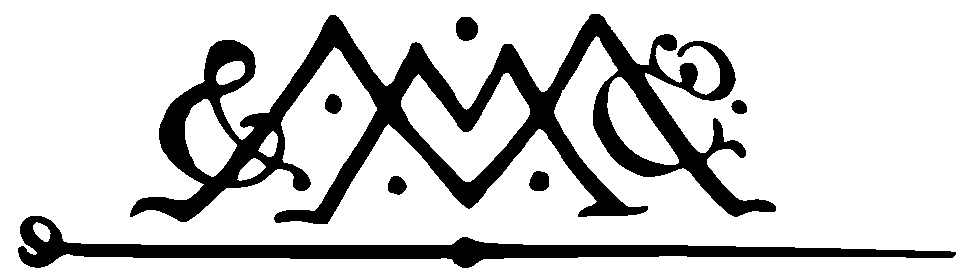
\includegraphics[height=1cm]{./images/macmillan2}
\vfil
\textit{\SMALL First Edition, Feb. $1892$. Reprinted, May, $1892$.}

\textit{\SMALL Second Edition, $1896$. Reprinted, $1905$.}

%% Note: the 1917 edition shows
%%   First Edition, February, 1892.
%%   Second Edition, May, 1892.
%%   Third Edition, 1896.
%%   Fourth Edition, 1905.
%%   Fifth Edition, 1911.
%%   Sixth Edition, 1914.
%%   Seventh Edition, 1917.
%% which provides a timeline more consistent with the "Note to the fourth edition" below!

\end{center}
\ifPaper\cleartorecto\else\newpage\fi
\endgroup
\ifPaper
  \frontmatter
\else
  \frontmatter*
\fi
\title{MATHEMATICAL\\
RECREATIONS AND ESSAYS}

\author{W.W. ROUSE BALL}
\affiliation{Fellow and Tutor of Trinity College, Cambridge.}
\Edition{FOURTH EDITION}

\Publisher{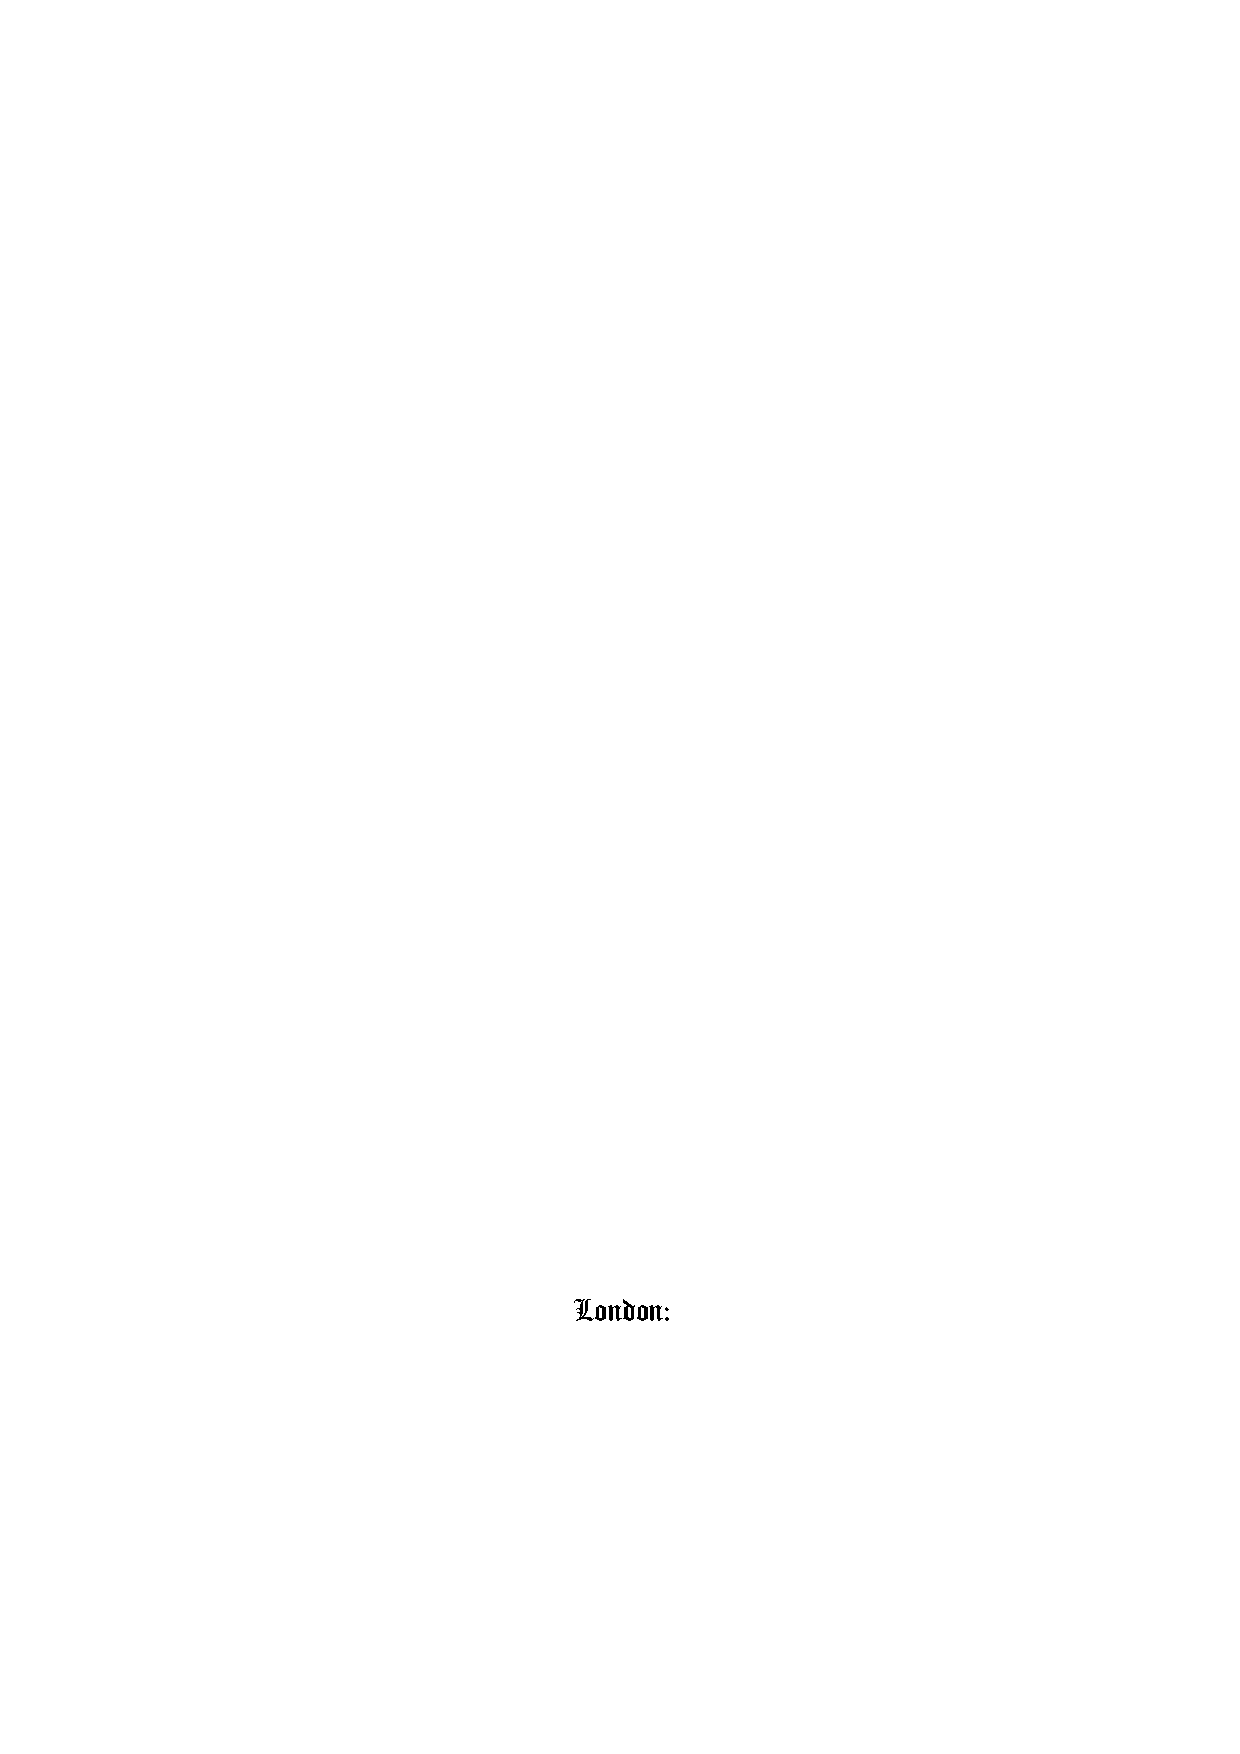
\includegraphics[width=49bp]{./images/london}\\ % blackletter text in image
MACMILLAN AND CO., Limited\\
\tiny NEW YORK: THE MACMILLAN COMPANY}
\date{1905}
\Rights{All rights reserved.}

\maketitle

\newpage

\ifEditorials\else
  \transcribersnote{Most of the open questions discussed by the author were
settled during the twentieth century.}
\fi

\transcribersnote{The author's footnotes are labelled using printer's
 marks\footnotemark; footnotes showing where corrections to the text
 have been made are labelled numerically\ifEditorials,
 as are explanatory notes\fi\footnotemarkT.}

\transcribersnote{\SMALL Minor typographical corrections are documented in the \LaTeX\ source.}


\makecopyrightpage
\ifPaper\cleartorecto\fi
\PGx---File: 002.png--------------------------------------------------
% MATHEMATICAL
% RECREATIONS AND ESSAYS
%
% BY
% W.W. ROUSE BALL
% FELLOW AND TUTOR OF TRINITY COLLEGE, CAMBRIDGE.
%
% \textit{FOURTH EDITION}
%
% London:
% MACMILLAN AND CO., LIMITED
% NEW YORK: THE MACMILLAN COMPANY
% 1905
% [\textit{All rights reserved.}]
%
\PGx---File: 003.png--------------------------------------------------
% \textit{First Edition, Feb. 1892. Reprinted, May, 1892
% Second Edition, 1896. Reprinted, 1905}.
\PGx---File: 004.png------------------------------------------------------

\chapter*[Preface]{PREFACE TO THE FIRST EDITION.}

{\advance\baselineskip1ex
\DPpdfbookmark[0]{Preface to the First Edition}{Preface*1}
\textsc{The} following pages contain an account of certain mathematical
recreations, problems, and speculations of past
and present times. I hasten to add that the conclusions are
of no practical use, and most of the results are not new. If
therefore the reader proceeds further he is at least forewarned.

At the same time I think I may assert that many of the
diversions---particularly those in the latter half of the book---are
interesting, not a few are associated with the names of
distinguished mathematicians, while hitherto several of the
memoirs quoted have not been easily accessible to English
readers.

The book is divided into two parts, but in both parts I have
included questions which involve advanced mathematics.

The \emph{\hyperlink{part.1}{first part}} consists of seven chapters, in which are
included various problems and amusements of the kind usually
called \emph{mathematical recreations}. The questions discussed in
the first of these chapters are connected with \hyperlink{chapter.1}{arithmetic}; those
in the second with \hyperlink{chapter.2}{geometry}; and those in the third relate to
\hyperlink{chapter.3}{mechanics}. The \hyperlink{chapter.4}{fourth chapter} contains an account of some
miscellaneous problems which involve both number and situation;
the \hyperlink{chapter.5}{fifth chapter} contains a concise account of magic
squares; and the \hyperlink{chapter.6}{sixth and seventh} chapters deal with some
\PG----File: 005.png-----------------------------------------------------
unicursal problems. Several of the questions mentioned in
the first three chapters are of a somewhat trivial character,
and had they been treated in any standard English work to
which I could have referred the reader, I should have pointed
them out. In the absence of such a work, I thought it best
to insert them and trust to the judicious reader to omit them
altogether or to skim them as he feels inclined.

The \emph{\hyperlink{part.2}{second part}} consists of five chapters, which are mostly
\emph{historical}. They deal respectively with \hyperlink{chapter.8}{three classical problems}
in geometry---namely, the duplication of the cube, the trisection
of an angle, and the quadrature of the circle---\hyperlink{chapter.10}{astrology},
the hypotheses as to the nature of \hyperlink{chapter.12}{space} and \hyperlink{chapter.14}{mass}, and a
means of \hyperlink{chapter.13}{measuring time}.

I have inserted detailed references, as far as I know, as
to the sources of the various questions and solutions given;
also, wherever I have given only the result of a theorem, I have
tried to indicate authorities where a proof may be found. In
general, unless it is stated otherwise, I have taken the references
direct from the original works; but, in spite of considerable
time spent in verifying them, I dare not suppose that they are
free from all errors or misprints.

I shall be grateful for notices of additions or corrections
which may occur to any of my readers.

}\bigskip
\vbox{\rightline{W.W. ROUSE BALL}
  \bigskip
  \setbox0=\hbox{\small\textsc{Trinity College, Cambridge.}}
  \setbox1=\hbox to\wd0{\small\hfil\textit{February}, 1892.\hfil}
  \indent\box0\par
  \indent\box1
}

\PG----File: 006.png-------------------------------------------------------

{\ifPaper\else\setlength{\beforechapskip}{0.75pc}\fi
\chapter*{NOTE TO THE FOURTH EDITION.}

\advance\baselineskip1ex
\DPpdfbookmark[0]{Note to the Fourth Edition}{Preface*2}
\textsc{In} this edition I have inserted in the earlier chapters
descriptions of several additional Recreations involving elementary
mathematics, and I have added in the second part
chapters on the \emph{History of the \hyperlink{chapter.7}{Mathematical Tripos} at Cambridge},
\emph{\hyperlink{chapter.9}{Mersenne's} \hyperlink{chapter.9}{Numbers}}, and \emph{\hyperlink{chapter.11}{Cryptography and Ciphers}}.

It is with some hesitation that I include in the book the
chapters on \emph{\hyperlink{chapter.10}{Astrology}} and \emph{\hyperlink{chapter.11}{Ciphers}}, for these subjects are only
remotely connected with Mathematics, but to afford myself
some latitude I have altered the title of the \hyperlink{part.2}{second part} to
\emph{Miscellaneous Essays and Problems}.

}\ifPaper\bigskip\else\smallskip\fi
\vbox{\rightline{W.W.R.B.}
  \ifPaper\bigskip\else\smallskip\fi
  \setbox0=\hbox{\small\textsc{Trinity College, Cambridge.}}
  \setbox1=\hbox to\wd0{\small\hfil13 \textit{May}, 1905.\hfil}
  \indent\box0\par
  \indent\box1
}

\PGx---File: 007.png----------------------------------------------------
\PGx---File: 008.png------------------------------------------------------
\PGx---File: 009.png------------------------------------------------------
\PGx---File: 010.png------------------------------------------------------
\PGx---File: 011.png------------------------------------------------------
\PGx---File: 012.png-------------------------------------------------------
\PGx---File: 013.png------------------------------------------------------
\PGx---File: 014.png-------------------------------------------------------
\PGx---File: 015.png------------------------------------------------------
\PG----File: 016.png-------------------------------------------------------
%ERRATA.
%
%Page 36, line 9. \emph{After} all \emph{insert} even. % [** fixed]
%
%Page 58, line 16. \emph{For} 13 \emph{read} 15. % [** fixed]
%
%Page 229, line 3. \emph{For} 1850 \emph{read} 1851. % [** fixed]
%
%Page 232, line 4. \emph{Before} 1854 \emph{insert} 1853 and. % [** fixed]
%
%Page 363, footnote \dag, and Page 364, footnote *.  \emph{These footnotes
%should be interchanged.} % [** fixed]
%
\PG----File: 017.png------------------------------------------------------

\clearpage
\DPpdfbookmark[0]{Table of Contents}{ToC*1}
\tableofcontents*

% now disable formatting commands used inside ToC, so bookmarks come out OK
% (could also use \pdfstringdefDisableCommands, but this is less work)
\let\tocsecbox\empty
\let\tocsecspacer\empty

\PG----File: 018.png------------------------------------------------------
\ifPaper
  \mainmatter
\else
  \mainmatter*
\fi
\pagestyle{mainstuff}

%PART I.
\PartQuote{``Les hommes ne sont jamais plus ingénieux que dans l'invention
des jeux; l'esprit s'y trouve à son aise\textellipsis. Après les jeux
qui dépendent uniquement des nombres viennent les jeux où
entre la situation\textellipsis. Après les jeux où n'entrent
que le nombre et la situation viendraient les jeux où entre
le mouvement\textellipsis. Enfin
il serait a souhaiter qu'on eût un cours entier des jeux, traités
mathématiquement.'' \hfill\qquad\penalty-1000\null\hfill
\hbox{\emph{(Leibnitz\index{Leibnitz on Games}: letter to De~Montmort\index
{DeMontmort@De Montmort}\index{Montmort, De}, July~29, 1715.)}}}
\part{\PartOneText}

\PGx---File: 019.png-------------------------------------------------------




%CHAPTER I.
\chapter[Some Arithmetical Questions.][Arithmetical Recreations.]%
{Some Arithmetical Questions.}

\textsc{The} interest excited by statements of the relations
between\chapindex{Arithmetical Recreations@\nobreak--- \textsc{Recreations}}
numbers of certain forms has been often remarked. The
majority of works on mathematical recreations include several
such problems, which are obvious to any one acquainted with
the elements of algebra, but which to many who are ignorant
of that subject possess the same kind of charm that some
mathematicians find in the more recondite propositions of
higher arithmetic. I shall devote the bulk of this chapter to
these elementary problems, but I append a few remarks on
one or two questions in the theory of numbers.

Before entering on the subject of the chapter, I may add
that a large proportion of the elementary questions mentioned
here and in the following two chapters are taken from one
of two sources. The first of these is the classical \textit{Problèmes
plaisans et délectables}, by C.G.~Bachet\index
{Bachet@Bachet's \textit  {Problèmes}|(}, sieur de Méziriac, of
which the first edition was published in 1612 and the second
in 1624: it is to the edition of 1624 that the references hereafter
given apply. Several of Bachet's problems are taken
from the writings of Alcuin\index{Alcuin}, Pacioli di~Burgo\index
{Lucas di Burgo}\index{Pacioli di Burgo}, Tartaglia\index{Tartaglia}, or
Cardan\index{Cardan}, and possibly some of them are of oriental origin,
but I have made no attempt to add such references. The
other source to which I alluded above is Ozanam's \textit{Récréations
mathématiques et physiques}\index
{Ozanam@Ozanam's \textit  {Récréations}}.
The greater portion of the original
edition, published in two volumes at Paris in 1694, was a
compilation from the works of Bachet, Leurechon\index{Leurechon},
Mydorge\index{Mydorge},
\PG----File: 020.png-------------------------------------------------------
van Etten\index{Etten, van}\index{VanEtten@Van Etten}, and Oughtred\index
{Oughtreds@Oughtred's \textit  {Recreations}}: this part is excellent,
but the
same cannot be said of the additions due to Ozanam\index
{Ozanam@Ozanam's \textit  {Récréations}}. In the
\textit{Biographie Universelle} allusion is made to subsequent editions
issued in 1720, 1735, 1741, 1778, and 1790; doubtless these
references are correct, but the following editions, all of which
I have seen, are the only ones of which I have any knowledge.
In 1696 an edition was issued at Amsterdam. In
1723---six years after the death of Ozanam---one was issued
in three volumes, with a supplementary fourth volume, containing
(among other things) an appendix on puzzles: I
believe that it would be difficult to find in any of the books
current in England on mathematical amusements as many as
a dozen puzzles which are not contained in one of these four
volumes. Fresh editions were issued in 1741, 1750 (the
second volume of which bears the date 1749), 1770, and
1790. The edition of 1750 is said to have been corrected
by Montucla\index{Montucla} on condition that his name should not be
associated with it; but the edition of 1790 is the earliest one
in which reference is made to these corrections, though the
editor is referred to only as Monsieur M***. Montucla\index{Montucla}
expunged most of what was actually incorrect in the older
editions, and added several historical notes, but unfortunately
his scruples prevented him from striking out the accounts of
numerous trivial experiments and truisms which overload the
work. An English translation of the original edition appeared
in 1708, and I believe ran through four editions, the last of
them being published in Dublin in 1790. Montucla's\index{Montucla} revision
of 1790 was translated by C.~Hutton\index{Hutton, C.}, and editions of this
were issued in 1803, in 1814, and (in one volume) in 1840:
my references are to the editions of 1803 and 1840.

\ThoughtBreakSpace

I proceed now to enumerate some of the elementary questions
connected with numbers which for nearly three centuries
have formed a large part of most compilations of mathematical
amusements. They are given here mainly for their historical---not
for their arithmetical---interest; and perhaps a mathematician
\PG----File: 021.png-----------------------------------------------------
may well omit them, and pass at once to the latter
part of this chapter.

These questions are of the nature of tricks or puzzles
and I follow the usual course and present them in that form.
I may note however that most of them are not worth proposing,
even as tricks, unless either the \textit{modus operandi} is
disguised or the result arrived at is different from that
expected; but, as I am not writing on conjuring, I refrain
from alluding to the means of disguising the operations
indicated, and give merely a bare enumeration of the steps
essential to the success of the method used, though I may
recall the fundamental rule that no trick, however good, will
bear immediate repetition, and that, if it is necessary to
appear to repeat it, a different method of obtaining the result
should be used.

\ssection[Elementary Questions on Numbers (Miscellaneous)]%
[Elementary Tricks and Problems]{To find a number selected by some one}
There are\index{Arithmetical Puzzles@\textsc{Arithmetical Puzzles}|(}%
\index{NumbersPuzzle@\nobreak--- \textsc{Puzzles with}|(}%
\index{PuzzlesArith@\textsc{Puzzles}, Arithmetical|(}%
\index{Tricks@\textsc{Tricks with Numbers}|(}
innumerable ways of finding a number chosen by some one,
provided the result of certain operations on it is known. I
confine myself to methods typical of those commonly used.
Any one acquainted with algebra will find no difficulty in
modifying the rules here given or framing new ones of an
analogous nature.

\subsection*{First Method\/\protect\footnote
{Bachet, \textit{Problèmes plaisans}, Lyons, 1624, problem~\textsc{i},
p.~53.}} (i)~Ask the person who has chosen the
number to treble it. (ii)~Enquire if the product is even or
odd: if it is even, request him to take half of it; if it is odd,
request him to add unity to it and then to take half of it.
(iii)~Tell him to multiply the result of the second step by $3$.
(iv)~Ask how many integral times $9$ divides into the latter
product: suppose the answer to be $n$. (v)~Then the number
thought of was $2n$ or $2n + 1$, according as the result of step (i)
was even or odd.

The demonstration is obvious. Every even number is of
the form $2n$, and the successive operations applied to this
give (i)~$6n$, which is even; (ii)~$\frac{1}{2}6n = 3n$; (iii)~$3 \times
 3n = 9n$;
(iv)~$\frac{1}{9}9n = n$; (v)~$2n$. Every odd number is of the form
\PG----File: 022.png------------------------------------------------------
$2n + 1$, and the successive operations applied to this give
(i)~$6n + 3$, which is odd; (ii)~$\tfrac{1}{2}(6n + 3 + 1) = 3n + 2$;
(iii)~$3 (3n + 2) = 9n + 6$; (iv)~$\tfrac{1}{9} (9n + 6) = n + \text
{a remainder}$;
(v)~$2n+1$. These results lead to the rule given above.

\subsection*{Second Method\/\protect\footnote
{A similar rule was given by Bachet, problem~\textsc{iv}, p.~74.
}} Ask the person who has chosen the
number to perform in succession the following operations.
(i)~To multiply the number by $5$. (ii)~To add $6$ to the product.
(iii)~To multiply the sum by $4$. (iv)~To add $9$ to the
product. (v)~To multiply the sum by $5$. Ask to be told the
result of the last operation: if from this product $165$ is subtracted,
and then the remainder is divided by $100$, the quotient
will be the number thought of originally.

For let $n$ be the number selected. Then the successive
operations applied to it give (i)~$5n$; (ii)~$5n + 6$; (iii)~$20n + 24$;
(iv)~$20n+33$; (v)~$100n+ 165$. Hence the rule.

\subsection*{Third Method\/\protect\footnote
{Bachet, problem~\textsc{v}, p.~80.}} Request the person who has thought of
the number to perform the following operations. (i)~To
multiply it by any number you like, say,~$a$. (ii)~To divide the
product by any number, say,~$b$. (iii)~To multiply the quotient
by~$c$. (iv)~To divide this result by~$d$. (v)~To divide the
final result by the number selected originally. (vi)~To add
to the result of operation (v) the number thought of at first.
Ask for the sum so found: then, if $ac/bd$ is subtracted from
this sum, the remainder will be the number chosen originally.

For, if $n$ was the number selected, the result of the first four
operations is to form $nac/bd$; operation (v) gives $ac/bd$; and
(vi) gives $n + (ac/bd)$, which number is mentioned. But $ac/bd$
is known; hence, subtracting it from the number mentioned,
$n$ is found. Of course $a$, $b$, $c$, $d$ may have any numerical values
it is liked to assign to them. For example, if $a =12$, $b = 4$,
$c = 7$, $d = 3$ it is sufficient to subtract $7$ from the final result
in order to obtain the number originally selected.

\subsection*{Fourth Method\/\protect\footnote
{\textit{Educational Times}, London, May~1, 1895, vol.~\textsc{xlviii},
p.~234.}} Ask some one to select a number less
\PG----File: 023.png-----------------------------------------------------
than $90$. (i)~Request him to multiply it by $10$, and to add
any number he pleases, $a$, which is less than $10$. (ii)~Request
him to divide the result of step (i) by $3$, and to mention the
remainder, say, $b$. (iii)~Request him to multiply the quotient
obtained in step (ii) by $10$, and to add any number he pleases,
$c$, which is less than $10$. (iv)~Request him to divide the result
of step (iii) by $3$, and to mention the remainder, say $d$, and
the third digit (from the right) of the quotient; suppose
this digit is $e$. Then, if the numbers $a$, $b$, $c$, $d$, $e$ are known,
the original number can be at once determined. In fact, if
the number is $9x + y$, where $x \ngtr 9$ and $y \ngtr 8$, and if $r$ is
the remainder when $a-b + 3 (c-d)$ is divided by $9$, we have
$x = e$, $y=9-r$.

The demonstration is not difficult. For if the selected
number is $9x + y$, step (i) gives $90x + 10y + a$; (ii)~let
$y + a = 3n + b$, then the quotient obtained in step (ii) is
$30x + 3y + n$; step (iii) gives $300x + 30y + 10n + c$; (iv)~let
$n + c = 3m + d$, then the quotient obtained in step (iv) is
$100x+ 10y+ 3n + m$, which I will denote by $Q$. Now the
third digit in $Q$ must be $x$, because, since $y\ngtr 8$ and $a \ngtr 9$,
we have $n \ngtr 5$; and since $n \ngtr 5$ and $c \ngtr 9$, we have
$m \ngtr 4$;
therefore $10y + 3n + m \ngtr 99$. Hence the third or hundreds
digit in $Q$ is $x$.

Again, from the relations $y + a = 3n + b$ and $n + c = 3m + d$,
we have $9m-y = a-b + 3(c-d)$: hence, if $r$ is the remainder
when $a-b +3(c-d)$ is divided by $9$, we have $y=9-r$. [This
is always true, if we make $r$ positive; but if $a-b + 3 (c-d)$
is negative, it is simpler to take $y$ as equal to its numerical
value; or we may prevent the occurrence of this case by
assigning proper values to $a$ and $c$.] Thus $x$ and $y$ are both
known, and therefore the number selected, namely $9x + y$, is
known.

\subsection*{Fifth Method\/\protect\footnote
{Bachet, problem~\textsc{vi}, p.~84: Bachet added, on p.~87, a note on the
previous history of the problem.
}} Ask any one to select a number less
than $60$. (i)~Request him to divide it by $3$ and mention the
\PG----File: 024.png------------------------------------------------------
remainder; suppose it to be $a$. (ii)~Request him to divide it
by $4$, and mention the remainder; suppose it to be $b$. (iii)~Request
him to divide it by $5$, and mention the remainder;
suppose it to be $c$. Then the number selected is the remainder
obtained by dividing $40a + 45b + 36c$ by $60$.

This method can be generalized and then will apply to any
number chosen. Let $a', b', c', \ldots$ be a series of numbers prime
to one another, and let $p$ be their product. Let $n$ be any
number less than $p$, and let $a, b, c, \ldots$ be the remainders
when $n$ is divided by $a', b', c', \ldots$ respectively. Find a number
$A$ which is a multiple of the product $b'c'd'\dotsm$ and which
exceeds by unity a multiple of $a'$. Find a number $B$ which
is a multiple of $a'c'd'\dotsm$ and which exceeds by unity a multiple
of $b'$; and similarly find analogous numbers $C, D, \dots$. Rules
for the calculation of $A, B, C, \ldots$ are given in the theory of
numbers, but in general, if the numbers $a', b', c', \ldots$ are small,
the corresponding numbers, $A, B, C, \ldots$ can be found by inspection.
I proceed to show that $n$ is equal to the remainder
when $Aa + Bb + Cc + \dotsb$ is divided by $p$.

Let $N = Aa + Bb + Cc + \dotsb$, and let $M(x)$ stand for a
multiple of $x$.

Now $A = M(a') + 1$, therefore $Aa = M(a') + a$. Hence, if
the first term in $N$, that is $Aa$, is divided by $a'$, the remainder
is $a$. Again, $B$ is a multiple of $a'c'd'\dotsm$. Therefore $Bb$ is
exactly divisible by $a'$. Similarly $Cc, Dd, \ldots$ are each exactly
divisible by $a'$. Thus every term in $N$, except the first, is
exactly divisible by $a'$. Hence, if $N$ is divided by $a'$, the
remainder is $a$. But if $n$ is divided by $a'$, the remainder is $a$.
\begin{LRalign}
Therefore & N-n &= M(a')\,.  \\
Similarly & N-n &= M(b')\,,  \\
          & N-n &= M(c')\,,  \\
          & \multispan{2}{\dotfill} \\
\indent But $a', b', c', \ldots$ are prime to one another.\\
&\Therefore N-n &= M(a'b'c' \dotsm)\rlap{${} = M(p)\,,$} \\
that is,&   N   &= M(p) + n\,.\\
\end{LRalign}
\PG----File: 025.png-------------------------------------------------------
Now $n$ is less than $p$, hence if $N$ is divided by $p$, the
remainder is $n$.

The rule given by Bachet corresponds to the case of $a' = 3$,
$b'= 4$, $c' = 5$, $p = 60$, $A = 40$, $B = 45$, $C = 36$. If the number
chosen is less than 420, we may take $a' = 3$, $b' = 4$, $c' = 5$, $d'= 7$,
$p = 420$, $A = 280$, $B = 105$, $C = 336$, $D = 120$.


\ssection*{To find the result of a series of operations performed
on any number (\emph{unknown to the questioner}) without asking
any questions} All rules for solving such problems ultimately
depend on so arranging the operations that the number disappears
from the final result. Four examples will suffice.

\subsection*{First Example\/\protect\footnote
{Bachet, problem~\textsc{viii}, p.~102.
}} Request some one to think of a number.
Suppose it to be $n$. Ask him (i)~to multiply it by any number
you please (say) $a$; (ii)~then to add (say) $b$; (iii)~then to divide
the sum by (say) $c$. (iv)~Next, tell him to take $a/c$ of the
number originally chosen; and (v)~to subtract this from the
result of the third operation. The result of the first three
operations is $(na + b)/c$, and the result of operation (iv) is
$na/c$: the difference between these is $b/c$, and therefore is
known to you. For example, if $a = 6$, $b = 12$, $c = 4$, and
$a/c = 1\frac{1}{2}$, then the final result is $3$.

\subsection*{Second Example\/\protect\footnote
{Bachet, problem~\textsc{xiii}, p.~123: Bachet presented the above trick in
a somewhat more general form, but one which is less effective in practice.
}} Ask $A$ to take any number of counters
that he pleases: suppose that he takes $n$ counters. (i)~Ask
some one else, say $B$, to take $p$ times as many, where $p$ is
any number you like to choose. (ii)~Request $A$ to give $q$ of
his counters to $B$, where $q$ is any number you like to select.
(iii)~Next, ask $B$ to transfer to $A$ a number of counters equal
to $p$ times as many counters as $A$ has in his possession. Then
there will remain in $B$'s hands $q (p + 1)$ counters: this number
is known to you; and the trick can be finished either by
mentioning it or in any other way you like.

The reason is as follows. The result of operation (ii) is
that $B$ has $pn + q$ counters, and $A$ has $n-q$ counters. The
\PG----File: 026.png-----------------------------------------------------
result of (iii) is that $B$ transfers $p(n-q)$ counters to $A$: hence
he has left in his possession $(pn + q)-p (n-q)$ counters, that
is, he has $q (p + 1)$.

For example, if originally $A$ took any number of counters,
then (if you chose $p$ equal to $2$), first you would ask $B$ to take
twice as many counters as $A$ had done; next (if you chose $q$
equal to $3$) you would ask $A$ to give $3$ counters to $B$; and
then you would ask $B$ to give to $A$ a number of counters equal
to twice the number then in $A$'s possession; after this was
done you would know that $B$ had $3 (2 + 1)$, that is, $9$ left.

This trick (as also some of the following problems) may be
performed equally well with one person, in which case $A$ may
stand for his right hand and $B$ for his left hand.

\subsection*{Third Example} Ask some one to perform in succession
the following operations. (i)~Take any number of three
digits. (ii)~Form a new number by reversing the order of
the digits. (iii)~Find the difference of these two numbers.
(iv)~Form another number by reversing the order of the digits
in this difference. (v)~Add together the results of (iii) and (iv).
Then the sum obtained as the result of this last operation will
be $1089$.

An illustration and the explanation of the rule are given
below.
\[
\begin{array}{crr@{}c@{}r@{}c@{}l}
\text{(i)}   &237   &100a        &{}+{}&10b    &{}+{}&c\\
\addlinespace
\text{(ii)}  &732   &100c        &{}+{}&10b    &{}+{}&a\\
\cmidrule(lr){2-2}\cmidrule(lr){3-7}
\text{(iii)} &495   &\multicolumn{1}{l@{}}{100(a-c-1)} &+&90     &+&(10+c-a)\\
\addlinespace
\text{(iv)}  &594   &\multicolumn{1}{l@{}}{100(10+c-a)} &+&90     &+&(a-c-1)\\
\cmidrule(lr){2-2}\cmidrule(lr){3-7}
\text{(v)}   &1089  &\multicolumn{1}{c}{900}        &+&180    &+&9\\
\cmidrule(lr){2-2}\cmidrule(lr){3-7}
\specialrule{0pt}{-1pt}{-1pt} % yes I know double rules are frowned upon!
\cmidrule(lr){2-2}\cmidrule(lr){3-7}
\end{array}
\]

\subsection*{Fourth Example\/\protect\footnote
{\textit{Educational Times Reprints}, 1890, vol.~\textsc{liii}, p.~78.}}
The following trick\index{Money, Question on|(} depends on the same
principle. Ask some one to perform in succession the following
operations. (i)~To write down any sum of money less than
\pounds12; the number of pounds not being the same as the number
of pence. (ii)~To \emph{reverse} this sum, that is, to write down a
\PG----File: 027.png------------------------------------------------------
sum of money obtained from it by interchanging the numbers
of pounds and pence. (iii)~To find the difference between the
results of (i) and (ii). (iv)~To reverse this difference. (v)~To
add together the results of (iii) and (iv). Then this sum will
be \pounds12.~18\textit{s}.~11\textit{d}.

For instance, take the sum \pounds10.~17\textit{s}.~5\textit{d}.; we have
\[
\begin{tabular}{rlrrr}
& & \pounds. & \textit{s}.& \textit{d}. \\
(i)   & \hbox to2cm{\dotfill} & 10 & 17 &  5 \\
\addlinespace
(ii)  & \dotfill &  5 & 17 & 10 \\
\cmidrule(lr){3-5}
(iii) & \dotfill &  4 & 19 &  7 \\
\addlinespace
(iv)  & \dotfill &  7 & 19 &  4 \\
\cmidrule(lr){3-5}
(v)   & \dotfill & 12 & 18 & 11 \\
\cmidrule(lr){3-5}
\specialrule{0pt}{-1pt}{-1pt} % yes I know double rules are frowned upon!
\cmidrule(lr){3-5}
\end{tabular}
\]

The following work explains the rule, and shows that the
final result is independent of the sum written down initially.
\[
\begin{tabular}{rlccc}
& & \pounds. & \textit{s}. & \textit{d}. \\
(i)   & \hbox to2cm{\dotfill} &  $a$  &  $b$  &  $c$ \\
\addlinespace
(ii)  & \dotfill &  $c$  &  $b$ &   $a$ \\
\cmidrule(lr){3-5}
(iii) & \dotfill & $a-c-\phantom{1}1$ & $\quad 19 \quad$ & $c-a+12$ \\
\addlinespace
(iv)  & \dotfill & $c-a + 12$ & $19$ & $a-c-\phantom{1}1$ \\
\cmidrule(lr){3-5}
(v)   & \dotfill &  $11$ &  $38$ &  $11$ \\
\cmidrule(lr){3-5}
\specialrule{0pt}{-1pt}{-1pt} % yes I know double rules are frowned upon!
\cmidrule(lr){3-5}
\end{tabular}
\]

The rule can be generalized to cover any system of monetary
units\index{Money, Question on|)}.

\ssection*{Problems involving Two Numbers} I proceed next to
give a couple of examples of a class of problems which involve
two numbers.

\subsection*{First Example\/\protect\footnote
{Bachet, problem~\textsc{ix}, p.~107.
}} Suppose that there are two numbers, one
even and the other odd, and that a person $A$ is asked to select
one of them, and that another person $B$ takes the other. It is
desired to know whether $A$ selected the even or the odd number.
Ask $A$ to multiply his number by 2 (or any even number) and
$B$ to multiply his by $3$ (or any odd number). Request them
\PG----File: 028.png-----------------------------------------------------
to add the two products together and tell you the sum. If it
is even, then originally $A$ selected the odd number, but if it is
odd, then originally $A$ selected the even number. The reason
is obvious.

\subsection*{Second Example\/\protect\footnote
{Bachet, problem~\textsc{xi}, p.~113.}}
The above rule was extended by Bachet
to any two numbers, provided they were prime to one another
and one of them was not itself a prime. Let the numbers be
$m$ and $n$, and suppose that $n$ is exactly divisible by $p$. Ask $A$
to select one of these numbers, and $B$ to take the other. Choose
a number prime to $p$, say $q$. Ask $A$ to multiply his number by
$q$, and $B$ to multiply his number by $p$. Request them to add
the products together and state the sum. Then $A$ originally
selected $m$ or $n$, according as this result is not or is divisible
by $p$. For example, $m = 7$, $n= 15$, $p = 3$, $q=2$.

\ssection*{Problems depending on the Scale of Notation} Many%
\index{Denary scale of notation}%
\index{Notation, Denary scale of}%
\index{Scale of Notation, Denary}%
\index{Scale Puzzles@\nobreak--- Puzzles dependent on|(}
of the rules for finding two or more numbers depend on the
fact that in arithmetic an integral number is denoted by
a succession of digits, where each digit represents the product
of that digit and a power of ten, and the number is equal
to the sum of these products. For example, $2017$ signifies
$(2 \times 10^3) + (0 \times 10^2) + (1 \times 10)+ 7$; that is, the $2$
represents
$2$ thousands, \IE\ the product of $2$ and $10^3$, the $0$ represents
$0$ hundreds, \IE\ the product of $0$ and $10^2$; the $1$ represents
$1$ ten, \IE\ the product of $1$ and $10$, and the $7$ represents
$7$ units. Thus every digit has a local value.

The application to tricks connected with numbers will be
understood readily from three illustrative examples.

\subsection*{First Example\/\protect\footnote
{Some similar questions were given by Bachet in problem~\textsc{xii}, p.~117;
by Oughtred\index{Oughtreds@Oughtred's \textit{Recreations}} in his \textit
{Mathematicall Recreations} (translated from or founded
on van Etten's\index{Etten, van}\index{VanEtten@Van Etten} work of 1633),
London, 1653, problem \textsc{xxxiv}; and by
Ozanam\index{Ozanam@Ozanam's \textit{Récréations}}, part~\textsc{i},
chapter~\textsc{x}.}}
A common conjuring trick is to ask a boy
among the audience to throw two dice, or to select at random
from a box a domino on each half of which is a number. The
boy is then told to recollect the two numbers thus obtained, to
\PG----File: 029.png----------------------------------------------------
choose either of them, to multiply it by $5$, to add $7$ to the
result, to double this result, and lastly to add to this the other
number. From the number thus obtained, the conjurer subtracts
$14$, and obtains a number of two digits which are the
two numbers chosen originally.

For suppose that the boy selected the numbers $a$ and $b$.
Each of these is less than ten---dice or dominoes ensuring this.
The successive operations give (i)~$5a$; (ii)~$5a + 7$; (iii)~$10a + 14$;
(iv)~$10a + 14 + b$. Hence, if 14 is subtracted from the final
result, there will be left a number of two digits, and these
digits are the numbers selected originally. An analogous
trick might be performed in other scales of notation if it was
thought necessary to disguise the process further.

\subsection*{Second Example\protect\footnote
{Bachet gave some similar questions in problem~\textsc{xii}, p.~117.}}
Similarly, if three numbers, say, $a$, $b$, $c$,
are chosen, then, if each of them is less than ten, they
can be found by the following rule. (i)~Take one of the
numbers, say, $a$, and multiply it by $2$. (ii)~Add $3$ to the
product; the result is $2a + 3$. (iii)~Multiply this by $5$, and
add $7$ to the product; the result is $10a + 22$. (iv)~To
this sum add the second number. (v)~Multiply the result
by $2$. (vi)~Add $3$ to the product. (vii)~Multiply by $5$, and
add the third number to the product. The result is
$100a+ 10b + c + 235$. Hence, if the final result is known, it
is sufficient to subtract $235$ from it, and the remainder will
be a number of three digits. These digits are the numbers
chosen originally.

I have seen a similar rule applied to determine the birthday
and age of some one in the audience. The result is a number
of six digits, of which the first two digits give the day of
the month, the middle two digits the number of the month,
and the last two digits the present age.

\subsection*{Third Example\protect\footnote
{A similar question was given by Laisant\index{Laisant, C.A.} and
Perrin\index{Perrin} in their \textit{Algèbre},
Paris, 1892; and in \textit{L'Illustration} for July~13, 1895.}}
The following rule for finding a man's
age is of the same kind. Take the tens digit of the year of
\PG----File: 030.png----------------------------------------------------
birth; (i)~multiply it by $5$; (ii)~to the product add $2$;
(iii)~multiply the result by $2$; (iv)~to this product add the
units digit of the birth-year; (v)~subtract the sum from $110$.
The result is the man's age in 1906.

The algebraic proof of the rule is obvious. Let $a$ and $b$ be
the tens and units digits of the birth-year. The successive
operations give (i)~$5a$; (ii)~$5a + 2$; (iii)~$10a + 4$ (iv)~$10a + 4 + b$;
(v)~$106 -(10a + b)$, which is his age in 1906. The rule can be
easily adapted to give the age in any specified year.

\ssection*{Other Problems with numbers in the denary scale}
I may mention here two or three other slight problems\index
{Denary scale of notation}
dependent on the common scale of notation, which, as far as I
am aware, are unknown to most compilers of books of puzzles.

\subsection*{First Problem} The first of them is as follows. Take any
number of three digits: reverse the order of the digits: subtract
the number so formed from the original number: then, if
the last digit of the difference is mentioned, all the digits in
the difference are known.

For let $a$ be the hundreds digit of the number chosen, $b$ be
the tens digit, and $c$ be the units digit. Therefore the number
is $100a + 10b +c$. The number obtained by reversing the digits
is $100c + 10b + a$. The difference of these numbers is equal to
$(100a + c)-(100c + a)$, that is, to $99 (a-c)$. But $a-c$ is not
greater than $9$, and therefore the remainder can only be $99$,
$198$, $297$, $396$, $495$, $594$, $693$, $792$, or $891$---in each case the
middle digit being $9$ and the digit before it (if any) being equal
to the difference between $9$ and the last digit. Hence, if the
last digit is known, so is the whole of the remainder.

\subsection*{Second Problem} The second problem is somewhat similar
and is as follows. (i)~Take any number; (ii)~reverse the
digits; (iii)~find the difference between the number formed in
(ii) and the given number; (iv)~multiply this difference by
any number you like to name; (v)~cross out any digit except
a nought; (vi)~read the remainder. Then the sum of the
digits in the remainder subtracted from the next highest multiple
of nine will give the figure struck out.
\PG----File: 031.png----------------------------------------------------

This follows at once from the fact that the result of operation
(iii)---and therefore also of operation (iv)---is necessarily a
multiple of nine, and it is known that the sum of the digits of
every multiple of nine is itself a multiple of nine\index
{Scale Puzzles@\nobreak--- Puzzles dependent on|)}.

\subsection*{Miscellaneous Questions} Besides these problems, properly
so called, there are numerous questions on numbers which can
be solved empirically, but which are of no special mathematical
interest.

As an instance I may quote a question which attracted
some attention in London in 1893, and may be enunciated
as follows. With the seven digits $9$, $8$, $7$, $6$, $5$, $4$, $0$ express
three numbers whose sum is $82$: each digit, being used
only once, and the use of the usual notations for fractions
being allowed. One solution is $80.6\dot{9} + .7\dot{4} + .\dot{5}$. Similar
questions are with the ten digits, $9$, $8$, $7$, $6$, $5$, $4$, $3$, $2$,
$1$, $0$, to
express numbers whose sum is unity; a solution is $35/70$ and
$148/296$. If the sum were $100$, a solution would be $50$, $49$, $1/2$,
% silently making $\frac{1}{2}$ look like the other fractions here
and $38/76$. A less straightforward question would be, with
the nine digits, $9$, $8$, $7$, $6$, $5$, $4$, $3$, $2$, $1$, to express four
numbers
whose sum is $100$; a solution is $78$, $15$, $\sqrt[2]{9}$, and
$\sqrt[3]{64}$.
% [*Note: the explicit "2" in the square root is necessary for the trick]

\ssection*{Problems with a series of things which are numbered}
Any collection of things which can be distinguished one from
the other---especially if numbered consecutively---afford easy
concrete illustrations of questions depending on these elementary
properties of numbers. As examples I proceed to
enumerate a few familiar tricks. The first two of these are
commonly shown by the use of a \emph{watch}, the last three are
best exemplified by the use of a \emph{pack of playing cards},
which readily lend themselves to such illustrations, and I
present them in these forms.

\subsection*{First Example\protect\footnote
{Bachet, problem~\textsc{xx}, p.~155; Oughtred\index
{Oughtreds@Oughtred's \textit{Recreations}},
\textit{Mathematicall Recreations},
London, 1653, p.~28.}}
The first of these examples\index{Watch Problem|(} is connected
with the hours marked on the face of a watch. In this
puzzle some one is asked to think of some hour, say, $m$, and
then to touch a number that marks another hour, say, $n$.
\PG----File: 032.png------------------------------------------------------
Then if, beginning with the number touched, he taps each
successive hour marked on the face of the watch, going in the
opposite direction to that in which the hands of the watch
move, and reckoning to himself the taps as $m$, $(m + 1)$,~\&c.,
the $(n +12)$th tap will be on the hour he thought of. For
example, if he thinks of \textsc{v} and touches \textsc{ix}, then, if he taps
successively \textsc{ix}, \textsc{viii}, \textsc{vii}, \textsc{vi},~\ldots,
going backwards and reckoning
them respectively as $5$, $6$, $7$, $8$,~\ldots, the tap which he
reckons as $21$ will be on the \textsc{v}.

The reason of the rule is obvious, for he arrives finally at
the $(n + 12-m)$th hour from which he started. Now, since he
goes in the opposite direction to that in which the hands of
the watch move, he has to go over $(n-m)$ hours to reach the
hour $m$: also it will make no difference if in addition he goes
over $12$ hours, since the only effect of this is to take him
once completely round the circle. Now $(n + 12-m)$ is always
positive, since $m<12$, and therefore if we make him pass over
$(n+12-m)$ hours we can give the rule in a form which is
equally valid whether $m$ is greater or less than $n$.

\subsection*{Second Example} The following is another well-known
way of indicating on a watch-dial an hour selected by some
one. I do not know who first invented it. If the hour is
tapped by a pencil beginning at \textsc{vii} and proceeding backwards
round the dial to \textsc{vi}, \textsc{v},~\&c., and if the person who
selected the number counts the taps, reckoning from the hour
selected (thus, if he selected \textsc{x}, he would reckon the first tap
as the $11$th), then the $20$th tap as reckoned by him will be on
the hour chosen.

For suppose he selected the $n$th hour. Then the $8$th tap
is on \textsc{xii} and is reckoned by him as the $(n + 8)$th. The tap
which he reckons as $(n + 9)$th is on \textsc{xi}, and generally the tap
which he reckons as $(n + p)$th is on the hour $(20-p)$. Hence,
putting $p-20-n$, the tap which he reckons as $20$th is on
the hour $n$. Of course the hours indicated by the first seven
taps are immaterial\index{Watch Problem|)}.

\subsection*{Extension}  It is obvious that the same trick can be
\PG----File: 033.png-----------------------------------------------------
performed with any collection of $m$ things, such as cards or
dominoes, which are distinguishable one from the other,
provided $m < 20$. For suppose the $m$ things are arranged on
a table in some numerical order, and the $n$th thing is selected
by a spectator. Then the first $(19-m)$ taps are immaterial,
the $(20-m)$th tap must be on the $m$th thing and be reckoned
by the spectator as the $(n + 20-m)$th, the $(20-m + 1)$th tap
must be on the $(m-1)$th thing and be reckoned as the
$(n + 20-m + 1)$th, and finally the $(20-n)$th tap will be on
the $n$th thing and is reckoned as the $20$th tap.

\subsection*{Third Example} The following example rests on an\index
{Cards, Problems with|(} \hypertarget{chapter:1:cards}
{extension} of the method used in the last question; it is
very simple, but I have never seen it previously described
in print. Suppose that a pack of $n$ cards is given to some
one who is asked to select one out of the first $m$ cards and to
remember (but not to mention) what is its number from the
top of the pack (say it is actually the $x$th card in the pack).
Then take the pack, reverse the order of the top $m$ cards
(which can be easily effected by shuffling), and transfer $y$ cards
(where $y < n-m$) from the bottom to the top of the pack.
The effect of this is that the card originally chosen is now the
$(y + m-x + 1)$th from the top. Return to the spectator the
pack so rearranged, and ask that the top card be counted as
the $(x + 1)$th, the next as the $(x+2)$th, and so on, in which
case the card originally chosen will be the $(y + m + 1)$th.
Now $y$ and $m$ can be chosen as we please, and may be varied
every time the trick is performed; thus any one unskilled in
arithmetic will not readily detect the \textit{modus operandi}.

\subsection*{Fourth Example\protect\footnote
{A particular case of this problem was
given by Bachet, problem~\textsc{xvii}, p.~138.}}
Place a card on the table, and on it
place as many other cards from the pack as with the number
of pips on the card will make a total of twelve. For example,
if the card placed first on the table is the five of clubs, then
seven additional cards must be placed on it. The court cards
may have any values assigned to them, but usually they are
\PG----File: 034.png----------------------------------------------------
reckoned as tens. This is done again with another card, and
thus another pile is formed. The operation may be repeated
either only three or four times or as often as the pack will
permit of such piles being formed. If finally there are $p$ such
piles, and if the number of cards left over is $r$, then the sum
of the number of pips on the bottom cards of all the piles will
be $13 (p - 4) + r$.

For, if $x$ is the number of pips on the bottom card of a
pile, the number of cards in that pile will be $13 - x$. A similar
argument holds for each pile. Also there are $52$ cards in the
pack; and this must be equal to the sum of the cards in the
$p$ piles and the $r$ cards left over.
\begin{align*}
\Therefore (13 - x_1) + (13 - x_2) + \dotsb + (13 - x_p) + r &= 52\,,\\
\Therefore 13p - (x_1 + x_2 + \dotsb + x_p) + r              &= 52\,,\\
\Therefore x_1 + x_2 + \dotsb + x_p                          &= 13p - 52 + r\\
                                                          &= 13 (p - 4) + r\,.
\end{align*}

More generally, if a pack of $n$ cards is taken, and if in each
pile the sum of the pips on the bottom card and the number of
cards put on it is equal to $m$, then the sum of the pips on the
bottom cards of the piles will be $(m + 1) p + r -n$. In an écarté
pack $n = 32$, and it is convenient to take $m = 15$.

\subsection*{Fifth Example} It may be noticed that cutting a pack\index
{Cutting Cards, Problems on}
of cards never alters the relative position of the cards provided
that, if necessary, we regard the top card as following immediately
after the bottom card in the pack. This is used in
the following trick\footnote
{Bachet, problem~\textsc{xix}, p.~152.}. Take a pack, and deal the cards face
upwards on the table, calling them one, two, three,~\&c.\ as you
put them down, and noting in your own mind the card first
dealt. Ask some one to select a card and recollect its number.
Turn the pack over, and let it be cut (not shuffled) as often as
you like. Enquire what was the number of the card chosen.
Then, if you deal, and as soon as you come to the original first
card begin (silently) to count, reckoning this as one, the
selected card will appear at the number mentioned. Of course,
\PG----File: 035.png----------------------------------------------------
if all the cards are dealt before reaching this number, you
must turn the cards over and go on counting continuously.

Another similar trick is performed by handing the pack
face upwards to some one, and asking him to select a card
and state its number, reckoning from the top; suppose it to
be the $n$th. Next, ask him to choose a number at which it
shall appear in the pack; suppose he selects the $m$th. Take
the pack and secretly move $m - n$ cards from the bottom to
the top (or if $n$ is greater than $m$, then $n - m$ from the top to
the bottom) and of course the card will be in the required
position\index{Cards, Problems with|)}.

\markright{Medieval Problems in Arithmetic.}
\section*{Medieval Problems in Arithmetic} Before leaving the\index
{Medieval Problems|(}
subject of these elementary questions, I may mention a few
problems which for centuries have appeared in nearly every
collection of mathematical recreations, and therefore may claim
what is almost a prescriptive right to a place here.

\subsection*{First Example\protect\footnote
{Some similar problems were given by Bachet, appendix, problem \textsc{iii},
p.~206; problem \textsc{ix}, p.~233; by Oughtred\index
{Oughtreds@Oughtred's \textit{Recreations}} in his \textit{Recreations},
p.~22: and by Ozanam\index{Ozanam@Ozanam's \textit{Récréations}}, 1803
edition, vol.~\textsc{i}, p.~174; 1840 edition, p.~79. Earlier
instances occur in Tartaglia's\index{Tartaglia} writings.}}
The following is a sample of one class
of these puzzles. Three men robbed a gentleman of a vase\index
{Vase Problem|(}, containing $24$ ounces of balsam. Whilst running away they
met in a wood with a glass-seller, of whom in a great hurry
they purchased three vessels. On reaching a place of safety
they wished to divide the booty, but they found that their
vessels contained $5$, $11$, and $13$ ounces respectively. How could
they divide the balsam into equal portions?

Problems like this can be worked out only by trial: there
are several solutions, of which one is as follows.
\[
\begin{tabularx}{\ifPaper.9\else.7\fi\textwidth}{l >{\centering}X
 >{\centering}X r @{}>{~}r @{ } l r @{ } l r @{ } l r @{ } l}
\multicolumn{4}{l@{}}{The vessels can contain\dotfill}     & 24 & oz.    &
 13 & oz.    & 11 & oz.    & 5 & oz.    \\
\multicolumn{4}{l@{}}{Their contents originally are~}       & 24 & \ldots &  0 &
 \ldots &  0 & \ldots & 0 & \ldots \\
\multicolumn{4}{l@{}}{First, make their contents\dotfill}  &  0 & \ldots &
  8 & \ldots & 11 & \ldots & 5 & \ldots \\
Second,      &       ''       &       ''       & \ldots & 16 & \ldots &  8 &
 \ldots &  0 & \ldots & 0 & \ldots \\
Third,       &       ''       &       ''       & \ldots & 16 & \ldots &  0 &
 \ldots &  8 & \ldots & 0 & \ldots \\
\PGx---File: 036.png----------------------------------------------------
Fourth,      &       ''       &       ''       & \ldots &  3 & \ldots & 13 &
 \ldots &  8 & \ldots & 0 & \ldots \\
Fifth,       &       ''       &       ''       & \ldots &  3 & \ldots &  8 &
 \ldots &  8 & \ldots & 5 & \ldots \\
Sixth,       &       ''       &       ''       & \ldots &  8 & \ldots &  8 &
 \ldots &  8 & \ldots & 0 & \ldots \\
\end{tabularx}\index{Vase Problem|)}
\]

\subsection*{Second Example\protect\footnote
{Bachet, problem~\textsc{xxii}, p.~170.}} The next of these is a not uncommon
game, played by two people, say $A$ and $B$. $A$ begins by
mentioning some number not greater than (say) six, $B$ may
add to that any number not greater than six, $A$ may add
to that again any number not greater than six, and so on.
He wins who is the first to reach (say) $50$. Obviously, if $A$
calls $43$, then whatever $B$ adds to that, $A$ can win next time.
Similarly, if $A$ calls $36$, $B$ cannot prevent $A$'s calling $43$ the
next time. In this way it is clear that the key numbers are
those forming the arithmetical progression $43$, $36$, $29$, $22$, $15$,
$8$, $1$; and whoever plays first ought to win.

Similarly, if no number greater than $m$ may be added at
any one time, and $n$ is the number to be called by the victor,
then the key numbers will be those forming the arithmetical
progression whose common difference is $m + 1$ and whose
smallest term is the remainder obtained by dividing $n$ by
$m + 1$.

The same game may be played in another form by placing
$n$ coins, matches, or other objects on a table, and directing
each player in turn to take away not more than $m$ of them.
Whoever takes away the last coin wins. Obviously the key
numbers are multiples of $m + 1$, and the first player who is
able to leave an exact multiple of $(m + 1)$ coins can win.
Perhaps a better form of the game is to make that player lose
who takes away the last coin, in which case each of the key
numbers exceeds by unity a multiple of $m + 1$.

Mr~Loyd\index{Loyd, S.} has also suggested\footnote
{\textit{Tit-Bits}, London, July~17, Aug.~7, 1897.} a modification which is
equivalent to placing $n$ counters in the form of a circle, and
allowing each player in succession to take away not more than
$m$ of them which are in unbroken sequence: $m$ being less than
\PG----File: 037.png---------------------------------------------------
$n$ and greater than unity. In this case the second of the two
players can always win.

\subsection*{Recent Extension of this Problem} The games last described
are very simple, but if we impose on the original problem the
additional restriction that each player may not add the same
number more than three times, the analysis becomes by no
means easy. It is difficult in this case to say whether it is an
advantage to begin or not. I have never seen this extension
described in print, and I will therefore enunciate it at length.

Suppose that each player is given eighteen cards, three of
them marked $6$, three marked $5$, three marked $4$, three
marked $3$, three marked $2$, and three marked $1$. They play
alternately; $A$ begins by playing one of his cards; then
$B$ plays one of his, and so on. He wins who first plays a
card which makes the sum of the points or numbers on all the
cards played exactly equal to $50$, but he loses if he plays
a card which makes this sum exceed $50$. The game can be
played mentally or by noting the numbers on a piece of paper,
and in practice it is unnecessary to use cards.

Thus, if they play as follows $A$,~$4$; $B$,~$3$; $A$,~$1$; $B$,~$6$; $A$,~$3$;
$B$,~$4$; $A$,~$4$; $B$,~$5$; $A$,~$4$; $B$,~$4$; $A$,~$5$; the game
stands at $43$.
$B$ can now win, for he may safely play $3$, since $A$ has not
another $4$ wherewith to follow it; and if $A$ plays less than $4$,
$B$ will win the next time. Again, if they play thus, $A$,~$6$;
$B$,~$3$; $A$,~$1$; $B$,~$6$; $A$,~$3$; $B$,~$4$; $A$,~$2$; $B$,~$5$;
$A$,~$1$; $B$,~$5$;
$A$,~$2$; $B$,~$5$; $A$,~$2$; $B$,~$3$; $A$ is now forced to play $1$, and
$B$ wins by playing~$1$.

The game can be also played if each player is given only
two cards of each kind.

\subsection*{Third Example} The following medieval problem\index
{Three-Things Problem|(} is somewhat
more elaborate. Suppose that three people, $P$, $Q$, $R$,
select three things, which we may denote by $a$, $e$, $i$, respectively,
and that it is desired to find by whom each object was
selected\footnote{Bachet, problem~\textsc{xxv}, p.~187.}.

Place $24$ counters on a table. Ask $P$ to take one counter,
\PG----File: 038.png-------------------------------------------------------
$Q$ to take two counters, and $R$ to take three counters. Next,
ask the person who selected $a$ to take as many counters as he
has already, whoever selected $e$ to take twice as many counters
as he has already, and whoever selected $i$ to take four times as
many counters as he has already. Note how many counters
remain on the table. There are only six ways of distributing
the three things among $P$, $Q$, and $R$; and the number of
counters remaining on the table is different for each way.
The remainders may be $1$, $2$, $3$, $5$, $6$, or $7$.

Bachet summed up the results in the mnemonic line
\emph{Par fer} ($1$) \emph{César} ($2$) \emph{jadis} ($3$)
\emph{devint} ($5$) \emph{si grand} ($6$) \emph{prince} ($7$).
Corresponding to any remainder is a word or words containing
two syllables: for instance, to the remainder $5$ corresponds
the word \emph{devint}. The vowel in the first syllable indicates the
thing selected by $P$, the vowel in the second syllable indicates
the thing selected by $Q$, and of course $R$ selected the remaining
thing. \emph{Salve certa animae semita vita quies} was suggested by
Oughtred\index{Oughtreds@Oughtred's \textit  {Recreations}}\footnote
{\textit{Mathematicall Recreations}, London, 1653, p.~20.
} as an alternative mnemonic line.

\subsection*{Extension} M.~Bourlet\index{Bourlet}, in the course of a very
kindly notice\footnote
{\textit{Bulletin des sciences mathématiques}, Paris, 1893,
vol.~\textsc{xvii}, pp.~105--107.} of the second edition of this work,
has given a much
neater solution of the above question, and has extended the
problem to the case of $n$ people, $P_0, P_1, P_2, \dotsc, P_{n-1}$, each of
whom selects one object, out of a collection of $n$ objects, such
as dominoes or cards. It is required to know which domino
or card was selected by each person.

Let us suppose the dominoes to be denoted or marked by
the numbers $0, 1, \dotsc, n-1$, instead of by vowels. Give one
counter to $P_1$, two counters to $P_2$, and generally $k$ counters to
$P_k$. Note the number of counters left on the table. Next
ask the person who had chosen the domino $0$ to take as many
counters as he had already, and generally whoever had chosen
the domino $h$ to take $n^h$ times as many dominoes as he had
already: thus if $P_k$ had chosen the domino numbered $h$, he
\PG----File: 039.png-------------------------------------------------------
would take $n^h k$ counters. Note the total number of counters
taken, \IE~$\textsum n^hk$. Divide it by $n$, then the remainder will be
the number on the domino selected by $P_0$; divide the quotient
by $n$, and the remainder will be the number on the domino
selected by $P_1$; divide this quotient by $n$, and the remainder
will be the number on the domino selected by $P_2$; and so on.
In other words, if the number of counters taken is expressed
in the scale of notation whose radix is $n$, then the $(h + 1)$th
digit from the right will give the number on the domino
selected by $P_h$.

Thus in Bachet's problem with $3$ people and $3$ dominoes,
we should first give one counter to $Q$, and two counters to $R$,
while $P$ would have no counters; then we should ask the
person who selected the domino marked $0$ or $a$ to take as
many counters as he had already, whoever selected the
domino marked $1$ or $e$ to take three times as many counters
as he had already, and whoever selected the domino marked
$2$ or $i$ to take nine times as many counters as he had already.
By noticing the original number of counters, and observing
that $3$ of these had been given to $Q$ and $R$, we should know
the total number taken by $P$, $Q$, and $R$. If this number
were divided by $3$, the remainder would be the number of the
domino chosen by $P$; if the quotient were divided by $3$ the
remainder would be the number of the domino chosen by $Q$;
and the final quotient would be the number of the domino
chosen by $R$\index{Three-Things Problem|)}.

I may add that Bachet also discussed the case when $n = 4$,
which had been previously considered by Diego Palomino\index{Diego Palomino}%
\index{Palomino} in
1599, but as M.~Bourlet's\index{Bourlet} method is general, it is unnecessary
to discuss further particular cases.

\subsection*{Decimation} The last of these antique problems to which\index
{Decimation|(}\label{page:DecimationStart}
I referred consists in placing men round a circle so that if
every $n$th man is killed the remainder shall be certain specified
individuals. When decimation was a not uncommon
punishment a knowledge of this kind may have had practical
interest.
\PG----File: 040.png-------------------------------------------------------

Hegesippus\index{Hegesippus on Decimation}\footnote
{\textit{De Bello Judaico}, bk.~\textsc{iii}, chaps.~16--18.
} says that Josephus\index{Josephus on Decimation} saved his life by such a
device. According to his account, after the Romans had
captured Jotopat, Josephus and forty other Jews took refuge
in a cave. Josephus, much to his disgust, found that all
except himself and one other man were resolved to kill themselves,
so as not to fall into the hands of their conquerors.
Fearing to show his opposition too openly he consented, but
declared that the operation must be carried out in an orderly
way, and suggested that they should arrange themselves round
a circle and that every third person should be killed until
but one man was left, who must then commit suicide. It is
alleged that he placed himself and the other man in the $31$st
and $16$th place respectively, with a result which will be easily
foreseen.

The question is usually presented in the following form. A
ship, carrying as passengers fifteen Turks and fifteen Christians,
encountered a storm, and the pilot declared that, in order to
save the ship and crew, one-half of the passengers must be
thrown into the sea. To choose the victims the passengers
were placed round a circle, and it was agreed that every ninth
man should be cast overboard, reckoning from a certain point.
It is desired to find an arrangement by which all the Christians
should be saved.\footnote
{Bachet, problem~\textsc{xxiii}, p.~174. The same problem had been
previously enunciated by Tartaglia\index{Tartaglia}.}

Problems like this can be easily solved by counting, but it
is impossible to give a general rule. In this case, the Christians,
reckoning from the man first counted, must occupy the
places $1$, $2$, $3$, $4$, $10$, $11$, $13$, $14$, $15$, $17$, $20$, $21$,
$25$, $28$, $29$.
This arrangement can be recollected by the positions of the
vowels in the following doggerel rhyme,
\begin{quote}
\emph{From numbers' aid and art, never will fame depart,}
\end{quote}
where $a$ stands for $1$, $e$ for $2$, $i$ for $3$, $o$ for $4$, and $u$ for
$5$.
Hence (looking only at the vowels in the verse) the order is
\PG----File: 041.png-------------------------------------------------------
$4$ Christians, $5$ Turks, $2$ Christians, $1$ Turk, $3$ Christians,
$1$ Turk, $1$ Christian, $2$ Turks, $2$ Christians, $3$ Turks, $1$ Christian,
$2$ Turks, $2$ Christians, $1$ Turk. Other similar mnemonic lines
in French and in Latin were given by Bachet\index
{Bachet@Bachet's \textit  {Problèmes}|)} and by Ozanam\index
{Ozanam@Ozanam's \textit  {Récréations}}
respectively\index{Decimation|)}\index{Medieval Problems|)}\index
{NumbersPuzzle@\nobreak--- \textsc{Puzzles with}|)}\label{page:DecimationEnd}.

\bigbreak
\section{Arithmetical Fallacies} I insert next some instances\index
{Arithmetical Fallacies|(}%
\index{FallaciesArith@\textsc{Fallacies, Arithmetical}|(}
of demonstrations\footnote
{Of the fallacies given in the text, the first, second, and third, are
well known; the fourth is not new, but the earliest work in which I
recollect seeing it is my \textit{Algebra}, Cambridge, 1890, p.~430; the fifth
is given in G.C.~Chrystal's \textit{Algebra}, Edinburgh, 1889,
vol.~\textsc{ii}, p.~159; the
eighth is due to G.T.~Walker\index{Walker, G.T.}, and, as far as I know, has
not appeared in
any other book; the ninth is due to D'Alembert\index{DAlembert@D'Alembert};
and the tenth to
F.~Galton\index{Galton}. A mechanical demonstration that $1 = 2$ was given by
R.~Chartres\index{Chartres, R.} in \textit{Knowledge}, July, 1891.
J.L.F.~Bertrand\index{Bertrand, J.L.F.} pointed out
that a demonstration that $1=-1$ can be also obtained from the proposition
in the Integral Calculus that, if the limits are constant, the order
of integration is indifferent; hence the integral to $x$
(from $x = 0$ to $x = 1$)
of the integral to $y$ (from $y = 0$ to $y =1$) of a function $\phi$ should
be equal
to the integral to $y$ (from $y = 0$ to $y = 1$) of the integral to $x$ (from
$x=0$ to $x = 1$) of $\phi$, but if $\phi=(x^2-y^2)/(x^2 + y^2)^2$, this gives
$\frac{1}{4}\pi =-\frac{1}{4}\pi$.} leading to arithmetical results which are
obviously impossible. I include algebraical proofs as well as
arithmetical ones. The fallacies are so patent that in preparing
the first and second editions I did not think such
questions worth printing, but, as some correspondents have
expressed a contrary opinion, I give them for what they are
worth.

\subsection*{First fallacy} One of the oldest of these---and not a very
interesting specimen---is as follows. Suppose that $a = b$, then
\begin{align*}
ab & =  a^2\,. \\
\Therefore ab-b^2 & =  a^2 - b^2\,. \\
\Therefore b(a-b) & =  (a+b)(a-b)\,. \\
\Therefore b & =  a + b\,. \\
\Therefore b & =  2b\,. \\
\Therefore 1 & =  2\,.
\end{align*}
\PG----File: 042.png-----------------------------------------------------

\subsection*{Second Fallacy} Another instance, almost as puerile, is as
follows. Let $a$ and $b$ be two unequal numbers, and let $c$ be
their arithmetic mean, hence
\begin{align*}
a + b &= 2c\,.\\
\Therefore (a + b)(a - b) &= 2c(a - b)\,.\\
\Therefore a^2 - 2ac &= b^2 - 2bc\,.\\
\Therefore a^2 - 2ac + c^2 &= b^2 - 2bc + c^2\,.\\
\Therefore (a - c)^2 &= (b - c)^2\,.\\
\Therefore a &= b\,.
\end{align*}

\subsection*{Third Fallacy} Another example, the idea of which is
due to John Bernoulli\index{Bernoulli, John}, may be stated as follows.
\begin{LRalign}
\indent We have & (-1)^2 &= 1\,.          \\
Take logarithms, & \Therefore 2 \log(-1) &= \log 1 = 0\,. \\
  & \Therefore   \log(-1) &= 0\,.          \\
  & \Therefore         -1 &= e^0\,.        \\
  & \Therefore         -1 &= 1\,.\\
\end{LRalign}

The same argument may be expressed thus. Let $x$ be a
quantity which satisfies the equation
\begin{LRalign}
&e^x &= -1\,.\\
Square both sides,&\Therefore e^{2x} &= 1\,.  \\
&\Therefore 2x &= 0\,.\\
&\Therefore x &= 0\,.\\
&\Therefore e^x &= e^0\,.\\
But $e^x = -1$ and $e^0 = 1$,& \Therefore -1 &= 1\,.\\
\end{LRalign}

\subsection*{Fourth Fallacy} As yet another instance, we know that
\[
  \log(1 + x) = x - \tfrac{1}{2}x^2 + \tfrac{1}{3}x^3 - \dotsb\,.
\]
If $x = 1$, the resulting series is convergent; hence we have
\begin{align*}
  \log 2 &= 1 - \tfrac{1}{2} + \tfrac{1}{3} - \tfrac{1}{4}
+ \tfrac{1}{5} - \tfrac{1}{6} + \tfrac{1}{7} - \tfrac{1}{8}
+ \tfrac{1}{9} - \dotsb\,.  \\
\Therefore 2 \log 2 &= 2 - 1 + \tfrac{2}{3} - \tfrac{1}{2}
+ \tfrac{2}{5} - \tfrac{1}{3} + \tfrac{2}{7} - \tfrac{1}{4}
+ \tfrac{2}{9} - \dotsb\,.
\end{align*}
\PG----File: 043.png-----------------------------------------------------
Taking those terms together which have a common denominator,
we obtain
\begin{LRalign}
&  2 \log 2 & =  1 + \frac{1}{3} - \frac{1}{2} + \frac{1}{5} +
  \frac{1}{7} - \frac{1}{4} + \frac{1}{9}-\dotsb \\ % inserted final -
&           & =  1 - \frac{1}{2} + \frac{1}{3} - \frac{1}{4} +
  \frac{1}{5}-\dotsb \\
&           & =  \log 2\,. \\
Hence&2 &= 1\,.\\
\end{LRalign}

\subsection*{Fifth Fallacy} This fallacy is very similar to that last
given. We have
\begin{align*}
  \log 2 & = \textstyle 1 - \frac{1}{2} + \frac{1}{3} - \frac{1}{4} +
  \frac{1}{5} - \frac{1}{6}+\dotsb \\
         & = \textstyle \left( 1 + \frac{1}{3} + \frac{1}{5} + \dotsb\right) -
  \left( \frac{1}{2} + \frac{1}{4}  + \frac{1}{6}+\dotsb\right) \\
         & = \textstyle \left \{  \left( 1 + \frac{1}{3} + \frac{1}{5}  +
  \dotsb \right)
  + \left( \frac{1}{2} + \frac{1}{4} + \frac{1}{6} + \dotsb\right)
  \right\} - 2 \left( \frac{1}{2}  + \frac{1}{4} + \frac{1}{6} +
  \dotsb \right) \\
         & = \textstyle \left\{ 1 + \frac{1}{2} + \frac{1}{3} + \dotsb\right\}
  - \left( 1 + \frac{1}{2} + \frac{1}{3} + \dotsb\right) \\
         & =  0\,.
\end{align*}

The error in each of the foregoing examples is obvious, but
the fallacies in the next examples are concealed somewhat
better.

\medskip
\subsection*{Sixth Fallacy} We can write the identity $\sqrt{-1} = \sqrt{-1}$
in the form
%
\begin{LRalign}
 & \sqrt{\frac{-1}{1}} & = \sqrt{\frac{1}{-1}}\, , \\
hence& \frac{\sqrt{-1}}{\sqrt{1}} & =  \frac{\sqrt{1}}{\sqrt{-1}} \, , \\
therefore& (\sqrt{-1})^2 & = (\sqrt{1})^2 \, , \\
that is,& -1 & = 1 \, .
\end{LRalign}

\subsection*{Seventh Fallacy} Again, we have
\begin{LRalign}
  &\sqrt{a} \times \sqrt{b} & = \sqrt{ab} \, . \\
\indent Hence& \sqrt{-1} \times \sqrt{-1} & = \sqrt{(-1) (-1)} \, , \\
therefore& (\sqrt{-1})^2 & =\sqrt{1} \, , \\
that is,& -1 & = 1 \, .
\end{LRalign}

\PG----File: 044.png-----------------------------------------------------
\subsection*{Eighth Fallacy}  The following demonstration depends on
the fact that an algebraical identity is true whatever be the
symbols used in it, and it will appeal only to those who are
familiar with this fact.

We have, as an identity,
\[
  \sqrt{x-y} = i \sqrt{y-x}
\tag{i}
\]
where $i$ stands either for $+ \sqrt{-1}$ or for $- \sqrt{-1}$. Now an
\emph{identity} in $x$ and $y$ is necessarily true whatever numbers $x$
and $y$ may represent. First put $x = a$ and $y = b$,
\[
  \Therefore \sqrt{a - b} = i \sqrt{b - a}
  \Tag{ii}
\]
 Next put $x = b$ and $y = a$,
\[
  \Therefore \sqrt{b - a} = i \sqrt{a - b}
  \Tag{iii}
\]
Also since (i) is an identity, it follows that in
(ii) and (iii) the symbol $i$ must be the same, that
is, it represents $+ \sqrt{-1}$ or $- \sqrt{-1}$ in both cases. Hence,
from (ii) and (iii), we have
\begin{LRalign}
 & \sqrt{a-b}\; \sqrt{b - a} & =  i^2 \sqrt{b-a}\; \sqrt{a - b}\,, \\
  &   \Therefore 1 & =  i^2\,, \\
that is& 1 &= -1 \, .
\end{LRalign}

\subsection*{Ninth Fallacy} The following fallacy is due to
D'Alembert\index{DAlembert@D'Alembert}\footnote
{\textit{Opuscules mathématiques}, Paris, 1761, vol.~\textsc{i},
p.~201.}. We know that if the product of two numbers is equal to the
product of two other numbers, the numbers will be in proportion, and
from the definition of a proportion it follows that if the first term
is greater than the second, then the third term will be greater than
the fourth: thus, if $ad=bc$, then $a:b = c:d$, and if in this
proportion $a > b$, then $c > d$. Now if we put $a = d =1$ and $b = c
= -1$ we have four numbers which satisfy the relation $ad = bc$ and such
that $a>b$; hence, by the proposition, $c > d$, that is, $-1 > 1$, which is
absurd.

\subsection*{Tenth Fallacy} The mathematical theory of probability\index
{Probabilities, Fallacies in} leads
to various paradoxes: of these one specimen\footnote{See \textit{Nature},
Feb.~15, March~1, 1894, vol.~\textsc{xlix}, pp.~365--366, 413.} will suffice.
\PG----File: 045.png-------------------------------------------------------
Suppose three coins to be thrown up and the fact whether each
comes down head or tail to be noticed. The probability that
all three coins come down head is clearly $(\frac{1}{2})^3$, that is,
is $\frac{1}{8}$;
similarly the probability that all three come down tail is $\frac{1}{8}$:
hence the probability that all the coins come down alike
(\IE\ either all of them heads or all of them tails) is $\frac{1}{4}$. But,
of three coins thus thrown up, at least two must come down alike;
now the probability that the third coin comes down head is $\frac{1}{2}$
and the probability that it comes down tail is $\frac{1}{2}$, thus the
probability that it comes down the same as the other two coins
is $\frac{1}{2}$: hence the probability that all the coins come down alike
is $\frac{1}{2}$. I leave to my readers to say whether either of these
conflicting conclusions is right and if so, which\index
{Arithmetical Fallacies|)}%
\index{FallaciesArith@\textsc{Fallacies, Arithmetical}|)}.

\subsection*{Arithmetical Problems} To the above examples I may add
the following questions, which I have often propounded in past
years: though not fallacies, they may serve to illustrate the
fact that the answer to an arithmetical question is frequently
different to what a hasty reader might suppose.

The first of these questions is as follows. Two clerks
are engaged, one at a salary commencing at the rate of (say)
\pounds100 a year with a rise of \pounds20 every year, the other at a
salary commencing at the same rate (\pounds100 a year) with a
rise of \pounds5 every half-year, in each case payments being made
half-yearly: which has the larger income? The answer is the
latter; for in the first year the first clerk receives \pounds100, but
the second clerk receives \pounds50 and \pounds55 as his two half-yearly
payments and thus receives in all \pounds105. In the second year
the first clerk receives \pounds120, but the second clerk receives
\pounds60 and \pounds65 as his two half-yearly payments and thus receives
in all \pounds125. In fact the second clerk will always receive
\pounds5 a year more than the first clerk.

As another question take the following. A man bets $1/n$th
of his money on an even chance (say tossing heads or tails
with a penny): he repeats this again and again, each time
betting $1/n$th of all the money then in his possession. If,
finally, the number of times he has won is equal to the number
\PG----File: 046.png-----------------------------------------------------
of times he has lost, has he gained or lost by the transaction?
He has, in fact, lost.

Here is another simple question to which not unfrequently
I have received incorrect answers. One tumbler is half-full
of wine, another is half-full of water: from the first tumbler
a teaspoonful of wine is taken out and poured into the
tumbler containing the water: a teaspoonful of the mixture
in the second tumbler is then transferred to the first tumbler.
As the result of this double transaction, is the quantity of
wine removed from the first tumbler greater or less than the
quantity of water removed from the second tumbler? Nineteen
people out of twenty will say it is greater, but this is not
the case\index{Tricks@\textsc{Tricks with Numbers}|)}.


\subsection*{Routes on a Chess-Board} A not uncommon problem\index
{Routes on a Chess-board} can
be generalised as\index{Chess-board, problems@\nobreak--- problems}
follows\footnote
{The substance of the problem was given in a scholarship paper set
at Cambridge about 30 years ago, and possibly was not new then.}.
Construct a rectangular board of
$mn$ cells (or small squares) by ruling $m+1$ vertical lines and
$n+1$ horizontal lines. It is required to know how many routes
can be taken from the top left-hand corner to the bottom right-hand
corner, the motion being along the ruled lines and its
direction being always either vertically downwards or horizontally
from left to right. The answer is $(m + n) ! / m! n !$: thus
on a square board containing $16$ cells (\IE\ one-quarter of a chess-board),
where $m=n = 4$, there are $70$ such routes; while on a
common chess-board, where $m=n=8$, there are no less than
12870 such routes. A similar theorem can be enunciated for
a parallelopiped.

Another problem of a somewhat similar type is the determination
of the number of closed routes through $mn$ points
arranged in $m$ rows and $n$ columns, following the lines of the
quadrilateral net-work, and passing once and only once through
each point\footnote
{See C.F.~Sainte-Marie in \textit{L'Intermédiaire des mathématiciens},
Paris, vol.~\textsc{xi}, March, 1904, pp.~86--88.}.

\markright{Permutation Problems.}
\subsection*{Permutation Problems} As other simple illustrations of\index
{Permutation Problems}
\PG----File: 047.png-----------------------------------------------------
the very large number of ways in which combinations of even
a few things can be arranged, I may note that as many as
$19,958400$ distinct skeleton cubes\index{Skeleton Cubes}\index
{Cubes, Skeleton} can be formed with twelve
differently coloured rods of equal
length\footnote{\textit{Mathematical Tripos}, Cambridge, Part~I,
1894.}; again there are
$3,979614,965760$ ways of arranging a set of twenty-eight
dominoes (\IE\ a set from double zero to double six) in a line,
with like numbers in contact\footnote
{Reiss\index{Reiss} in \textit{Annali di matematica},
Milan, November, 1871, vol.~\textsc{v}, pp.~63--120.}; while there are no less
than $53644,737765,488792,839237,440000$ possible different distributions
of hands at whist\index{Whist, Number of Hands at}\index
{Cards, Problems with} with a pack of fifty-two
cards\footnote{That is $(52!)/(13!)^4$.}.

\subsection*{Voting Problems} Here is a simple example on combinations
dealing with the cumulative vote\index{Cumulative Vote}\index
{Voting, Question on} as affecting the
representation of a minority. If there are $p$ electors each
having $r$ votes of which not more than $s$ may be given to one
candidate, and $n$ men are to be elected, then the least number
of supporters who can secure the election of a candidate must
exceed $pr/(ns + r)$.

\subsection*{Exploration Problems} Another common question is concerned\index
{Exploration Problems}
with the maximum distance into a desert which could
be reached from a frontier settlement by the aid of a party of
$n$ explorers, each capable of carrying provisions that would last
one man for $a$ days. The answer is that the man who reaches
the greatest distance will occupy $na/(n + 1)$ days before he
returns to his starting point. If in the course of their
journey they may make depôts, the longest possible journey
will occupy $\frac{1}{2}a (1 + \frac{1}{2} + \frac{1}{3}+ \dotsb + 1/n)$ days.
Further extensions by the use of horses and cycles will suggest themselves.

\ThoughtBreakSpace
Here I conclude my account of such of these easy problems\index
{Arithmetical Puzzles@\textsc{Arithmetical Puzzles}|)}
on numbers or elementary algebra as seemed worth reproducing.
It will be noticed that the majority of them either are due to
Bachet or were collected by him in his classical \textit{Problèmes}\index
{Bachet@Bachet's \textit  {Problèmes}|(}; but
it should be added that besides the questions I have mentioned
\PG----File: 048.png-----------------------------------------------------
he enunciated, even if he did not always solve, some other
problems of greater interest. One instance will suffice.

\ssection[Bachet's Weights Problem]{Bachet's Weights Problem\protect\footnote
{Bachet, Appendix,
problem~\textsc{v}, p.~215.}} Among the more difficult\index
{Weights@\textsc{Weights Problem, the}|(}
problems proposed by Bachet was the determination of the
least number of weights which would serve to weigh any
integral number of pounds from $1$~lb.\ to $40$~lbs.\ inclusive.
Bachet gave two solutions: namely, (i)~the series of weights
of $1$, $2$, $4$, $8$, $16$, and $32$~lbs.; (ii)~the series of weights of
$1$, $3$, $9$, and $27$~lbs.

If the weights may be placed in only one of the scale-pans,
the first series gives a solution, as had been pointed out in
1556 by Tartaglia\index{Tartaglia}\footnote
{\textit{Trattato de' numeri e misure}, Venice,
1556, vol.~\textsc{ii}, bk.~\textsc{i}, chap.~\textsc{xvi}, art.~32.}.

Bachet, however, assumed that any weight might be
placed in either of the scale-pans. In this case the second
series gives the least possible number of weights required. His
reasoning is as follows. To weigh $1$~lb.\ we must have a $1$~lb.\
weight. To weigh $2$~lbs.\ we must have in addition either a
$2$~lb.\ weight or a $3$~lb.\ weight; but, if we are confined to only
one new weight (in addition to the $1$~lb.\ we have got already),
then with no weight greater than $3$~lbs.\ could we weigh $2$~lbs.:
if we use a $2$~lb.\ weight we then can weigh $1$~lb., $2$~lbs., and
$3$~lbs., but if we use a $3$~lb.\ weight we then can weigh $1$~lb.,
$(3-1)$~lbs., $3$~lbs., and $(3 + 1)$~lbs.; hence a $3$~lb.\ weight is
preferable. Similarly, to enable us to weigh $5$~lbs.\ we must have
another weight not greater than $9$~lbs., and a weight of $9$~lbs.\
enables us to weigh every weight from $1$~lb.\ to $13$~lbs.; hence
it is the best to choose. The next weight required will be
$2(1 + 3 + 9) + 1$~lb., that is, will be $27$~lbs.; and this enables
us to weigh from $1$~lb.\ to $40$~lbs.\ Thus only four weights are
required, namely, $1$~lb., $3$~lbs., $3^2$~lbs., and $3^3$~lbs.

We can show similarly that the series of weights of $1$, $3$,
$3^2$, $\dots$, $3^{n-1}$~lbs.\ will enable us to weigh any integral number
of pounds from $1$~lb.\ to $(1+3 + 3^2+ \dotsb 3^{n-1})$~lbs., that is, to
\PG----File: 049.png-----------------------------------------------------
$\frac{1}{2}(3^n-1)$~lbs. This is the least number with which the problem
can be effected.

To determine the arrangement of the weights to weigh any
given mass we have only to express the number of pounds in
it as a number in the ternary scale of notation, except that in
finding the successive digits we must make every remainder
either $0$, $1$, or $-1$: to effect this a remainder $2$ must be written
as $3-1$, that is, the quotient must be increased by unity, in
which case the remainder is $-1$. This is explained in most
text-books on algebra.

Bachet's argument does not prove that his result is unique
or that it gives the least possible number of weights required.
These omissions have been supplied by Major MacMahon\index{MacMahon|(},
who has discussed the far more difficult problem (of which
Bachet's is a particular case) of the determination of all possible
sets of weights, not necessarily unequal, which enable us to
weigh any integral number of pounds from $1$ to $n$ inclusive,
(i)~when the weights may be placed in only one scale-pan, and
(ii)~when any weight may be placed in either scale-pan. He
has investigated also the modifications of the results which are
necessary when we impose either or both of the further conditions
(\textit{a})~that no other weighings are to be possible, and
 (\textit{b})~that
each weighing is to be possible in only one way, that is, is to
be unique\footnote
{See his article in the \textit{Quarterly Journal of Mathematics}, 1886,
vol.~\textsc{xxi}, pp.~367--373. An account of the method is given in
\textit{Nature}, Dec.~4, 1890, vol.~\textsc{xlii}, pp.~113--114.}.

The method for case (i) consists in resolving $1 + x + x^2 + \dotsb + x^n$
into factors, each factor being of the form $1 + x^a+ x^{2a} + \dotsb +x^{ma}$;
the number of solutions depends on the composite character of
$n + 1$. The method for case (ii) consists in resolving the expression
$x^{-n} + x^{-n+1}+ \dotsb\allowbreak + x^{-1} + 1 + x + \dotsb\allowbreak
 + x^{n-1} + x^n$ into factors,
each factor being of the form $x^{-ma} + \dotsb\allowbreak
 + x^{-a} + 1 + x^a+ \dotsb + x^{ma}$;
the number of solutions depends on the composite character of
$2n+1$.

Bachet's problem falls under case (ii), $n = 40$. MacMahon's
\PG----File: 050.png-----------------------------------------------------
analysis shows that there are eight such ways of factorizing
$x^{-40} + x^{-39} +\allowbreak\dotsb\allowbreak+ 1 + x^{39} + x^{40}$.
First, there is the
expression itself in which $a=1$, $m= 40$. Second, the expression is
equal to $(1-x^{81})/x^{40} (1-x)$, which can be resolved into the
product of $(1-x^3)/x (1-x)$ and $(1-x^{81})/x^{39} (1-x^3)$; hence it
can be resolved into two factors of the form given above, in
one of which $a=1$, $m=1$, and in the other, $a =3$, $m=13$.
Third, similarly, it can be resolved into two such factors, in
one of which $a=1$, $m = 4$, and in the other $a = 9$, $m = 4$.
Fourth, it can be resolved into three such factors, in one of
which $a = 1$, $m= 1$, in another $a = 3$, $m = 1$, and in the other,
$a = 9$, $m = 4$. Fifth, it can be resolved into two such factors,
in one of which $a = 1$, $m = 13$, and in the other $a = 27$, $m = 1$.
Sixth, it can be resolved into three such factors, in one of
which $a=1$, $m = 1$, in another $a = 3$, $m = 4$, and in the other
$a = 27$, $m = 1$. Seventh, it can be resolved into three such
factors, in one of which $a = 1$, $m= 4$, in another $a = 9$, $m=1$,
and in the other $a= 27$, $m=1$. Eighth, it can be resolved
into four such factors, in one of which $a= 1$, $m= 1$, in another
$a = 3$, $m = 1$, in another $a = 9$, $m = 1$, and in the other $a = 27$,
$m= 1$.

These results show that there are eight possible sets of
weights with which any integral number of pounds from $1$ to
$40$ can be weighed subject to the conditions (ii), (\textit{a}), and
(\textit{b}).
If we denote $p$ weights each equal to $w$ by $w^p$, these eight
solutions are $1^{40}$; $1$, $3^{13}$; $1^4$, $9^4$; $1$, $3$, $9^4$;
$1^{13}$, $27$; $1$, $3^4$, $27$;
$1^4$, $9$, $27$; $1$, $3$, $9$, $27$.
The last of these is Bachet's\index{Bachet@Bachet's \textit  {Problèmes}|)}
solution: not only is it that in which the least number of weights are
employed, but it is also the only unique one in which all the
weights are unequal%
\index{MacMahon|)}%
\index{PuzzlesArith@\textsc{Puzzles}, Arithmetical|)}%
\index{Weights@\textsc{Weights Problem, the}|)}.

\section{Problems in Higher Arithmetic}  At the commencement%
\index{Arithmetic, Higher@\textsc{Arithmetic, Higher}|(}%
\index{Higher@\textsc{Higher Arithmetic}|(}%
\index{NumbersTheory@\nobreak--- \textsc{Theory of}|(}
of this chapter I alluded to the special interest which
many mathematicians find in the theorems of higher arithmetic:
such, for example, as that every prime of the form
$4n+1$ and every power of it is expressible as the sum of two
\PG----File: 051.png------------------------------------------------------
squares\footnote{Fermat's\index{Fermat, P.} \textit{Diophantus}, Toulouse,
1670, bk.~\textsc{iii}, prop.~22, p.~127; or
Brassinne's \textit{Précis}, Paris, 1853, p.~65.},
and the first and second powers can be expressed
thus in only one way. For instance, $13 = 3^2 + 2^2$,
$13^2 = 12^2 + 5^2$,
$13^3 = 46^2 + 9^2$, and so on. Similarly $41 = 5^2 + 4^2$,
$41^2 = 40^2 + 9^2$,
$41^3 = 236^2+115^2$, and so on.

Propositions such as the one just quoted may be found in
text-books on the theory of numbers and therefore lie outside
the limits of this work, but there are one or two questions in
higher arithmetic involving points not yet quite cleared up
which may find a place here.

\ssection*{Primes} The first of these is concerned with the possibility
of determining readily whether a given number is prime\index
{Primes@\textsc{Primes}} or
not. Euler\index{Euler} and Gauss\index{Gauss} attached great importance to
this problem, but failed to establish any conclusive test. It would
seem, however, that Fermat\index{Fermat, P.} possessed some means of finding
from its form whether a given number (at any rate if one of
certain known forms) was prime or not. Thus, in answer to
Mersenne\index{Mersenne on Primes} who asked if he could tell without much
trouble whether the number $100895,598169$ was a prime, Fermat wrote
on April~7, 1643, that it was the product of $898423$ and $112303$,
both of which were primes. I have indicated elsewhere one
way by which this result can be found, and Mr~F.W.~Laurence
has indicated another which may have been that used by
Fermat in this particular case.

\markright{Mersenne's Numbers.}
\ssection*{Mersenne's Numbers\protect\footnote
{For references, see \protect\hyperlink{chapter.9}{chapter~ix} below.}}
Another illustration, confirmatory\index
{MersenneNos@\textsc{Mersenne's Numbers}|(}\DPlabel{Mersenne:I}
of the opinion that Fermat or some of his contemporaries had
a test by which it was possible to find out whether certain
numbers were prime, may be drawn from Mersenne's \textit{Cogitata
Physico-Mathematica} which was published in 1644. In the
preface to that work it is asserted that in order that $2^p-1$
may be prime, the only values of $p$, not greater than $257$,
which are possible are $1$, $2$, $3$, $5$, $7$, $13$, $17$, $19$, $31$, $67$,
$127$, and $257$: I conjecture that the number $67$ is a misprint
for $61$. With this correction the statement appears to be
\PG----File: 052.png------------------------------------------------------
true\Editorial
{It's not: see \href{http://www.mersenne.org}{www.mersenne.org}},
and it has been verified for all except nineteen values
of $p$: namely, $71$, $101$, $103$, $107$, $109$, $137$, $139$, $149$, $157$,
$163$, $167$, $173$, $181$, $193$, $199$, $227$, $229$, $241$, and $257$. Of
these values, Mersenne asserted that $p = 257$ makes $2^p-1$
a prime, and that the other values make $2^p-1$ a composite
number. The demonstrations for the cases when $p = 89$, $127$
have not been published; nor have the actual factors of $2^p-1$
when $p = 89$ been as yet determined: the discovery of these
factors may be commended to those interested in the theory
of numbers.

Mersenne's result could not be obtained empirically, and it
is impossible to suppose that it was worked out for every case;
hence it would seem that whoever first enunciated it was
acquainted with certain theorems in higher arithmetic which
have not been re-discovered\index{MersenneNos@\textsc{Mersenne's Numbers}|)}.

\markright{Perfect Numbers.}
\ssection*{Perfect Numbers\protect\footnote
{On the theory of perfect numbers, see bibliographical references by
H.~Brocard, \textit{L'Intermédiaire des mathématiciens}, Paris, 1895,
vol.~\textsc{ii}, pp.~52--54; and 1905, vol.~\textsc{xii}, p.~19.}}
The theory of \emph{perfect numbers}\index{Perfect@\textsc{Perfect Numbers}}
depends directly on that of Mersenne's Numbers. A number is
said to be perfect if it is equal to the sum of all its integral
subdivisors. Thus the subdivisors of $6$ are $1$, $2$, and $3$; the
sum of these is equal to $6$; hence $6$ is a perfect number.

It is probable that all perfect numbers are included in the
formula $2^{p-1} (2^p-1)$, where $2^p-1$ is a prime. Euclid\index{Euclid}
proved that any number of this form is perfect; Euler\index{Euler} showed
that the formula includes all even perfect numbers; and there is
reason to believe---though a rigid demonstration is wanting---that
an odd number cannot be perfect. If we assume that the
last of these statements is true, then every perfect number is
of the above form. It is easy to establish that every number
included in this formula (except when $p = 2$) is congruent to
unity to the modulus $9$, that is, when divided by $9$ leaves a
remainder $1$; also that either the last digit is a $6$ or the last
two digits are $28$.

Thus, if $p = 2$, $3$, $5$, $7$, $13$, $17$, $19$, $31$, $61$, then by
 Mersenne's rule
\PG----File: 053.png------------------------------------------------------
the corresponding values of $2^p-1$ are prime; they are $3$, $7$, $31$,
$127$, $8191$, $131071$, $524287$, $2147483647$, $2305843009213693951$;
and the corresponding perfect numbers are $6$, $28$, $496$, $8128$,
$33550336$, $8589869056$, $137438691328$, $2305843008139952128$,
and \hfil\allowbreak\hfilneg$2658455991569831744654692615953842176$.

\markright{Goldbach's Theorem.}
\ssection*{Goldbach's Theorem} Another interesting problem\index
{Goldbach's Theorem} in
higher arithmetic is the question whether there are any even
integers which cannot be expressed as a sum of two primes.
Probably there are none. The expression of all even\footnoteT
{`even' inserted as per errata sheet} integers not
greater than $5000$ in the form of a sum of two primes has
been effected\footnote{\textit{Transactions of the Halle Academy
 (Naturforschung)}, vol.~\textsc{lxxii},
Halle, 1897, pp.~5--214: see also \textit{L'Intermédiaire des
mathématiciens}, 1903, vol.~\textsc{x}, and 1904, vol.~\textsc{xi}.},
but a general demonstration that all even
integers can be so expressed is wanting.

\markright{Lagrange's Theorem.}
\ssection*{Lagrange's Theorem\protect\footnote
{\textit{Nouveaux Mémoires de l'Académie Royale des Sciences}, Berlin,
1775, p.~356.}}
Another theorem in higher arithmetic\index{Lagrange's Theorem}
which, as far as I know, is still unsolved, is to the effect
that every prime of the form $4n - 1$ is the sum of a prime of
the form $4n + 1$ and of double a prime of the form $4n + 1$;
for example, $23 = 13 + 2 \times 5$. Lagrange, however, added that
it was only by induction that he arrived at the result.

\ssection*{Fermat's Theorem on Binary Powers}%
\addcontentsline{toc}{subsection}{Fermat's \protect\textit{Theorem on
 Binary Powers}}%
\markright{Fermat's Theorem on Binary Powers.}%
Fermat\label{page:Fermat}%
\index{Binary@\textsc{Binary Powers}, Fermat on|(}%
\index{Fermat, P.|(}%
\index{Fermat on Binary Powers|(} enriched
mathematics with a multitude of new propositions.
With two exceptions all these have been proved subsequently
to be true. The first of these exceptions is his \emph{theorem on
binary powers}, in which he asserted that all numbers of the
form $2^m + 1$, where $m = 2^n$, are primes\footnote
{Letter of Oct.~18, 1640, \textit{Opera}, Toulouse, 1679, p.~162: or
Brassinne's \textit{Précis}, p.~143.},
but he added that,
though he was convinced of the truth of this proposition, he
could not obtain a valid demonstration.

It may be shown that $2^m +1$ is composite if $m$ is not a
power of $2$, but of course it does not follow that $2^m + 1$ is a
prime if $m$ is a power of $2$. As a matter of fact the theorem
\PG----File: 054.png-----------------------------------------------------
is not true. In 1732
Euler\index{Euler}\footnote
{\textit{Commentarii Academiae Scientiarum Petropolitanae}, St Petersburg,
1738, vol.~\textsc{vi}, p.~104; see also \textit
{Novi Comm. Acad. Sci. Petrop.}, St Petersburg,
1764, vol.~\textsc{ix}, p.~101: or \textit
{Commentationes Arithmeticae Collectae},
St Petersburg, 1849, vol.~\textsc{i}, pp.~2, 357.}
showed that if $n = 5$ the formula
gives $4294,967297$, which is equal to $641 \times 6,700417$: curiously
enough, these factors can be deduced at once from Fermat's\index
{Binary@\textsc{Binary Powers}, Fermat on|)}\index{Fermat on Binary Powers|)}
remark on the possible factors of numbers of the form $2^m \pm 1$,
from which it may be shown that the prime factors (if any)
of $2^{32} + 1$ must be primes of the form $64n + 1$.

During the last thirty years it has been
shown\footnote{For the factors and bibliographical references, see the memoir
by A.J.C.~Cunningham\index{Cunningham, A.J.C.} and A.E.~Western\index
{Western on Binary Powers}, \textit{Transactions of the London
Mathematical Society}, May~14, 1903, series~2, vol.~\textsc{i}, p.~175.}
that the
resulting numbers are composite when $n = 6$, $9$, $11$, $12$, $18$, $23$,
$36$, and $38$: the two last numbers contain many thousands of
millions of digits. I believe that Eisenstein\index{Eisenstein} asserted that
the number of primes of the form $2^m + 1$, where $m = 2^n$, is infinite:
the proof has not been published, but perhaps it might throw
some light on the general theory.

\ssection*{Fermat's Last Theorem}%
\addcontentsline{toc}{subsection}{Fermat's \protect\textit{Last Theorem}}%
\markright{Fermat's Last Theorem.}%
I pass now to the only other
assertion made by Fermat which has not been proved hitherto\Editorial
{Andrew Wiles' proof appeared in 1995: \textit{Annals of Mathematics},
vol.~\textsc{cxli}, pp.~443--551}.
This, which is sometimes known as \textit{Fermat's Last Theorem}\index
{FermatsLast@\textsc{Fermat's Last Theorem}|(}, is
to the effect\footnote
{Fermat's enunciation will be found in his edition of \textit{Diophantus},
Toulouse, 1670, bk.~\textsc{ii}, qu.~8, p.~61; or Brassinne's
\textit{Précis}, Paris, 1853,
p.~53. For bibliographical references, see \textit{L'Intermédiaire des
mathématiciens}, 1905, vol.~\textsc{xii}, pp.~11, 12.}
that no integral values of $x$, $y$, $z$ can be found
to satisfy the equation $x^n + y^n = z^n$, if $n$ is an integer greater
than $2$. This proposition has acquired extraordinary celebrity
from the fact that no general demonstration of it has been
given, but there is no reason to doubt that it is true.

Fermat seems to have discovered its truth first\footnote
{See a letter from Fermat quoted in my \textit{History of Mathematics},
London, chapter~\textsc{xv}.}
for the case
$n = 3$, and then for the case $n = 4$. His proof for the former
of these cases is lost, but that for the latter is
extant\footnote{Fermat's \textit{Diophantus}, note on p.~339;
or Brassinne's \textit{Précis}, p.~127.}, and a
\PG----File: 055.png-----------------------------------------------------
similar proof for the case of $n=3$ was given by
Euler\index{Euler}\footnote{Euler's Algebra (English trans. 1797),
vol.~\textsc{ii}, chap.~\textsc{xv}, p.~247.}. These
proofs depend upon showing that, if three integral values of
$x$, $y$, $z$ can be found which satisfy the equation, then it will be
possible to find three other and smaller integers which also
satisfy it: in this way finally we show that the equation must
be satisfied by three values which obviously do not satisfy it.
Thus no integral solution is possible. It would seem that this
method is inapplicable except when $n = 3$ and $n = 4$.

Fermat's discovery of the general theorem was made later.
An easy demonstration can be given on the assumption that
every number can be resolved into prime (complex) factors in
one and only one way. That assumption has been made by
some writers, but it is not universally true. It is possible that
Fermat made some such supposition, though it is perhaps more
probable that he discovered a rigorous demonstration. At any
rate he asserts definitely that he had a valid proof---demonstratio
mirabilis sane---and the fact that every other theorem
on the subject which he stated he had proved has been subsequently
verified must weigh strongly in his favour; especially
as in making the one statement in his writings which is not
correct he was scrupulously careful to add that he could not
obtain a satisfactory demonstration of it.

It must be remembered that Fermat was a mathematician
of quite the first rank who had made a special study of the
theory of numbers. That subject is in itself one of peculiar
interest and elegance, but its conclusions have little practical
importance, and since his time it has been discussed by only
a few mathematicians, while even of them not many have made
it their chief study. This is the explanation of the fact that
it took more than a century before some of the simpler results
which Fermat had enunciated were proved, and thus it is not
surprising that a proof of the theorem which he succeeded in
establishing only towards the close of his life should involve
great difficulties.

\PG----File: 056.png-----------------------------------------------------
In 1823 Legendre\index{Legendre}\footnote
{Reprinted in his \textit{Théorie des Nombres}, Paris, 1830,
vol.~\textsc{ii}, pp.~361--368: see also pp.~5, 6.}
obtained a proof for the case of $n = 5$;
in 1832 Lejeune Dirichlet\index{Dirichlet on Fermat's Theorem}\index
{Lejeune Dirichlet on Fermat}\footnote
{\textit{Crelle's Journal}, 1832, vol.~\textsc{ix}, pp.~390--393.}
gave one for $n=14$, and in 1840
Lamé\index{Lame@Lamé} and Lebesgue\index
{Lebesgue on Fermat's Theorem}\footnote
{\textit{Liouville's Journal}, 1841, vol.~\textsc{v}, pp.~195--215,
276--9, 348--9.} gave proofs for $n=7$.

The proposition appears to be true universally, and in 1849
Kummer\index{Kummer on Fermat's Theorem}\footnote
{References to Kummer's Memoirs are given in Smith's\index
{Smith, H@\protect\nobreak--- Hen., on Numbers} Report to
the British Association on the Theory of Numbers, London, 1860.},
by means of ideal primes, proved it to be so for all
numbers except those (if any) which satisfy three conditions.
It is not known whether any number can be found to satisfy
these conditions, but it seems unlikely, and it has been shown
that there is no number less than $100$ which does so. The
proof is complicated and difficult, and there can be little
doubt is based on considerations unknown to Fermat. I
may add that to prove the truth of the proposition when $n$ is
greater than $4$, it obviously is sufficient to confine ourselves to
cases where $n$ is a prime, and the first step in Kummer's
demonstration is to show that in such cases one of the numbers
$x$, $y$, $z$ must be divisible by $n$.

Naturally there has been much speculation as to how Fermat
arrived at the result. The modern treatment of higher
arithmetic is founded on the special notation and processes
introduced by Gauss\index{Gauss}, who pointed out that the theory of
discrete magnitude is essentially different from that of continuous
magnitude, but until the end of the last century the
theory of numbers was treated as a branch of algebra, and such
proofs by Fermat as are extant involve nothing more than
elementary geometry and algebra, and indeed some of his
arguments do not involve any symbols. This has led some
writers to think that Fermat used none but elementary
algebraic methods. This may be so, but the following remark,
which I believe is not generally known, rather points to the
opposite conclusion. He had proposed, as a problem to the
\PG----File: 057.png-----------------------------------------------------
English mathematicians, to show that there was only one
integral solution of the equation $x^2 + 2 = y^3$: the solution
evidently being $x = 5, y = 3$. On this he has a
note\footnote{Fermat's \textit{Diophantus}, bk.~\textsc{vi}, prop.~19,
p.~320; or Brassinne's \textit{Précis}, p.~122.} to the
effect that there was no difficulty in finding a solution in
rational fractions, but that he had discovered an entirely new
method---sane pulcherrima et subtilissima---which enabled him
to solve such questions in integers. It was his intention to
write a work\footnote{Fermat's \textit{Diophantus}, bk.~\textsc{iv},
prop.~31, p.~181; or Brassinne's \textit{Précis}, p.~82.}
on his researches in the theory of numbers, but
it was never completed, and we know but little of his methods
of analysis. I venture however to add my private suspicion
that continued fractions played a not unimportant part in his
researches, and as strengthening this conjecture I may note
that some of his more recondite results---such as the theorem
that a prime of the form $4n + 1$ is expressible as the sum of
two squares---may be established with comparative ease by
properties of such fractions%
\index{Arithmetic, Higher@\textsc{Arithmetic, Higher}|)}%
\index{Fermat, P.|)}%
\index{FermatsLast@\textsc{Fermat's Last Theorem}|)}%
\index{Higher@\textsc{Higher Arithmetic}|)}%
\index{NumbersTheory@\nobreak--- \textsc{Theory of}|)}.

\PG----File: 058.png-----------------------------------------------------


%CHAPTER II.

\chapter{Some Geometrical Questions.}

\textsc{In} this chapter I propose to enumerate certain geometrical\chapindex
{Geometrical Recreations@\textsc{Geometrical Recreations}}
questions the discussion of which will not involve necessarily
any considerable use of algebra or arithmetic. Unluckily no
writer like Bachet has collected and classified problems of this
kind, and I take the following instances from my note-books
with the feeling that they represent the subject but imperfectly.

The first part of the chapter is devoted to questions which
are of the nature of formal propositions: the last part contains
a description of various trivial puzzles and games, which the
older writers would have termed geometrical, but which the
reader of to-day may omit without loss.

In accordance with the rule I laid down for myself in the
preface, I exclude the detailed discussion of theorems which
involve advanced mathematics. Moreover (with one possible
exception) I exclude also any mention of the numerous geometrical
paradoxes which depend merely on the inability of the
eye to compare correctly the dimensions of figures when their
relative position is changed. This apparent deception does
not involve the conscious reasoning powers, but rests on the
inaccurate interpretation by the mind of the sensations derived
through the eyes, and I do not consider such paradoxes as
coming within the domain of mathematics.

\PG----File: 059.png-----------------------------------------------------
\section{Geometrical Fallacies} Most educated Englishmen are%
\index{FallaciesGeom@\nobreak--- \textsc{Geometrical}|(}%
\index{Geometrical Fallacies@\textsc{Geometrical Fallacies}|(}
acquainted with the series of logical propositions in geometry
associated with the name of Euclid\index{Euclid}, but it is not known so
generally that these propositions were supplemented originally
by certain exercises. Of such exercises Euclid issued three
series: two containing easy theorems or problems, and the
third consisting of geometrical fallacies, the errors in which
the student was required to find.

The collection of fallacies prepared by Euclid\index{Euclid} is lost, and
tradition has not preserved any record as to the nature of the
erroneous reasoning or conclusions; but, as an illustration of
such questions, I append two or three demonstrations, leading
to obviously impossible results, which perhaps may amuse any
one to whom they are new. I leave the discovery of the errors
to the ingenuity of my readers.

\subsection*{First Fallacy}  \emph{To prove that a right angle is equal to an
angle which is greater than a right angle.} Let $ABCD$ be a
rectangle. From $A$ draw a line $AE$ outside the rectangle,
equal to $AB$ or $DC$ and making an acute angle with $AB$, as
\begin{figure*}[!hbt]
\centerline{\ifpdf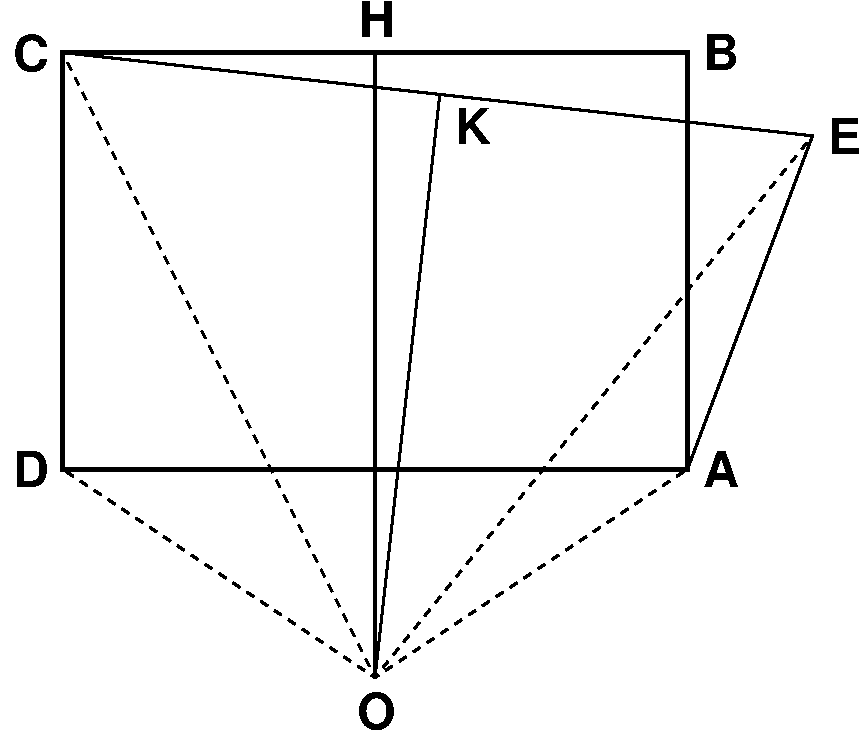
\includegraphics[height=6.5cm,viewport=0 0 415 350]{./images/illus059.pdf} % size graphic using BoundingBox
  \else\includegraphics[height=6.5cm]{./images/illus059.eps}\fi}
\end{figure*}
indicated in the diagram. Bisect $CB$ in $H$, and through $H$
draw $HO$ at right angles to $CB$. Bisect $CE$ in $K$, and through
$K$ draw $KO$ at right angles to $CE$. Since $CB$ and $CE$ are not
\PG----File: 060.png-----------------------------------------------------
parallel the lines $HO$ and $KO$ will meet (say) at $O$. Join $OA$,
$OE$, $OC$, and $OD$.

The triangles $ODC$ and $OAE$ are equal in all respects.
For, since $KO$ bisects $CE$ and is perpendicular to it, we have
$OC= OE$. Similarly, since $HO$ bisects $CB$ and $DA$ and is perpendicular
to them, we have $OD = OA$. Also, by construction,
$DC = AE$. Therefore the three sides of the triangle $ODC$ are
equal respectively to the three sides of the triangle $OAE$.
Hence, by Euc.~\textsc{i}.~8, the triangles are equal; and therefore the
angle $ODC$ is equal to the angle $OAE$.

Again, since $HO$ bisects $DA$ and is perpendicular to it, we
have the angle $ODA$ equal to the angle $OAD$.

Hence the angle $ADC$ (which is the difference of $ODC$ and
$ODA$) is equal to the angle $DAE$ (which is the difference of
$OAE$ and $OAD$). But $ADC$ is a right angle, and $DAE$ is
necessarily greater than a right angle. Thus the result is
impossible.

\subsection*{Second Fallacy\protect\footnote
{See a note by M.~Coccoz\index{Coccoz} in \textit{L'Illustration}, Paris,
 Jan.~12, 1895.}}
\emph{To prove that a part of a line is equal to
the whole line.} Let $ABC$ be a triangle; and, to fix our ideas,
let us suppose that the triangle is scalene, that the angle $B$ is
\begin{figure*}[!hbt]
\centerline{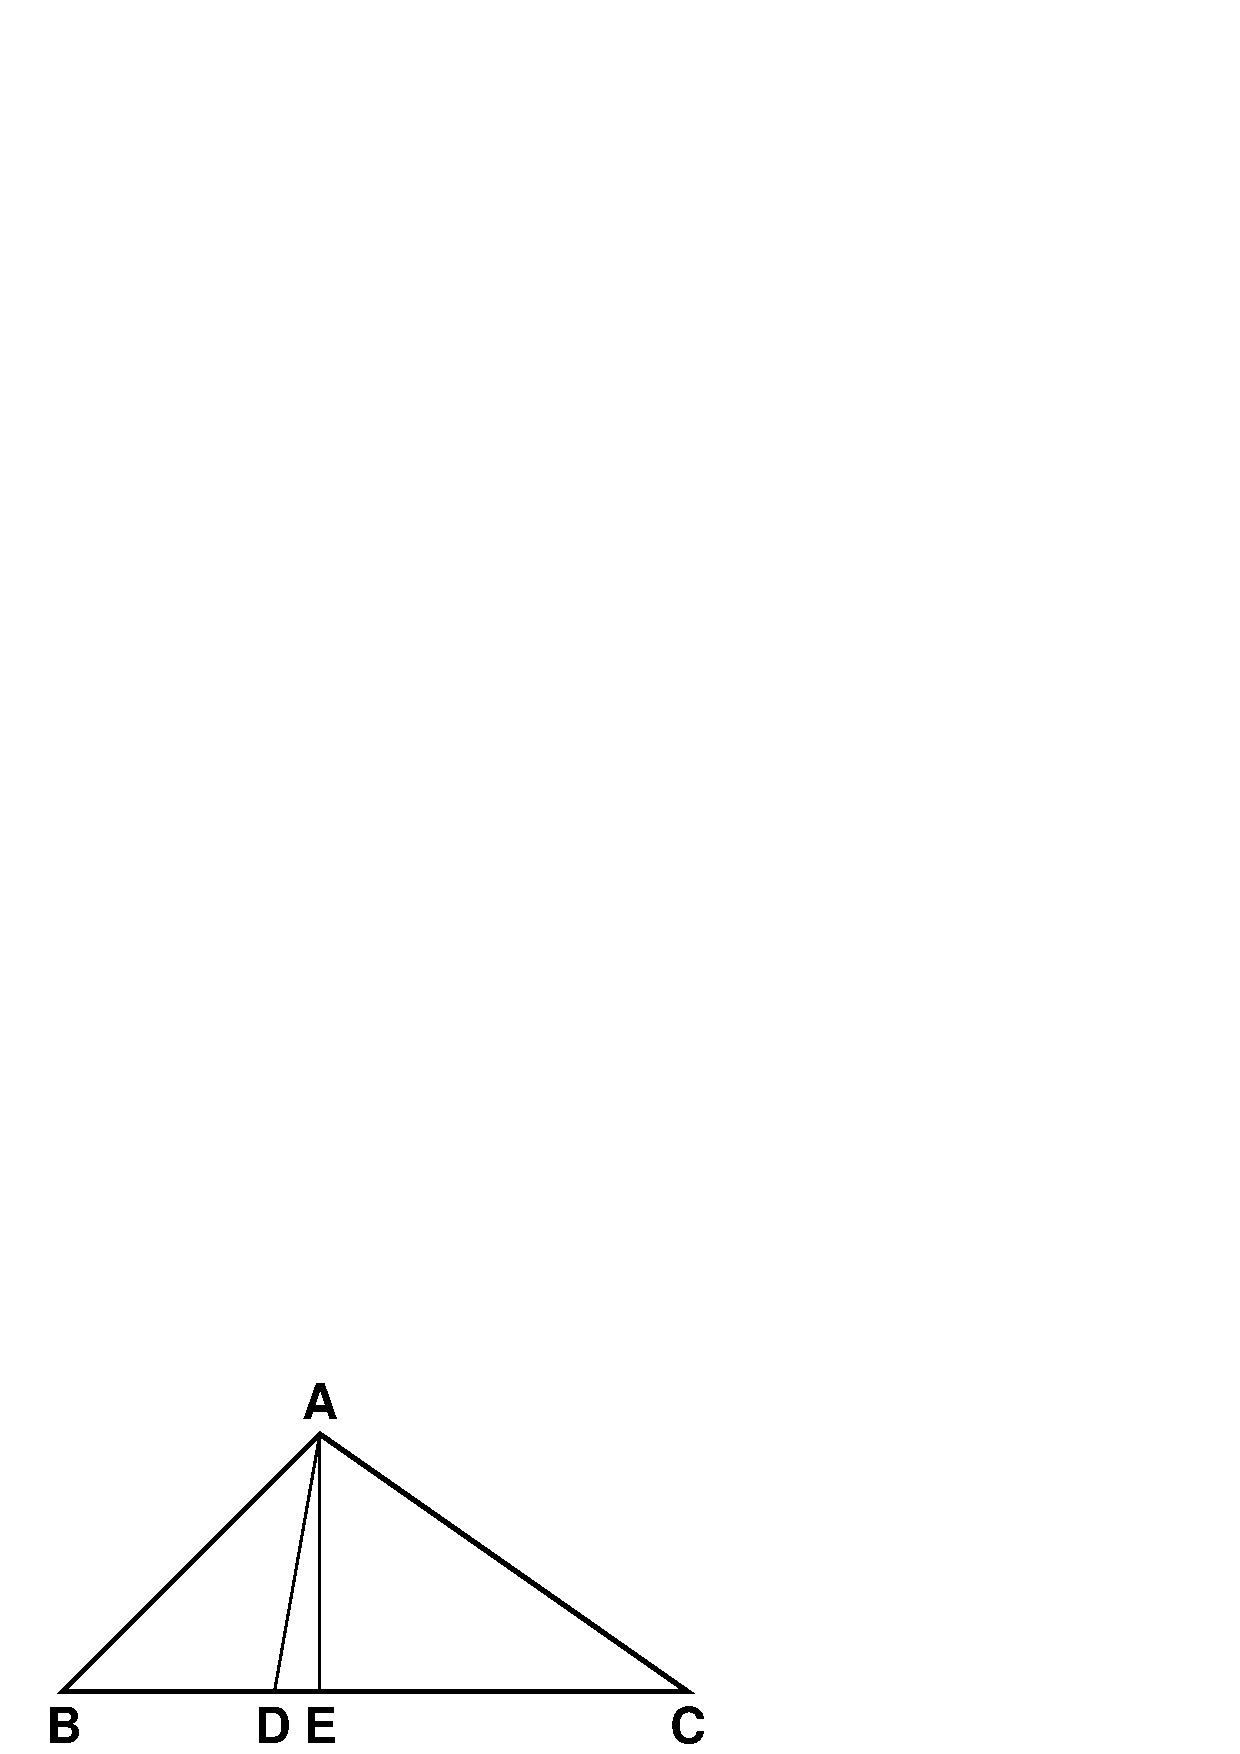
\includegraphics[height=3.3cm]{./images/illus060}}
\end{figure*}
acute, and that the angle $A$ is greater than the angle $C$. From
$A$ draw $AD$ making the angle $BAD$ equal to the angle $C$, and
cutting $BC$ in $D$. From $A$ draw $AE$ perpendicular to $BC$.

The triangles $ABC$, $ABD$ are equiangular; hence, by Euc.~\textsc{vi}.~19,
% slight alteration: using displayed equation
\[
\triangle ABC : \triangle ABD = AC^2 : AD^2\,.
\]
\PG----File: 061.png------------------------------------------------------
Also the triangles $ABC$, $ABD$ are of equal altitude: hence, by
Euc.~\textsc{vi}.~1,
\begin{align*}
  \triangle ABC : \triangle ABD &= BC : BD\,, \\
  \Therefore AC^2 : AD^2 &= BC : BD\,. \\
  \Therefore \frac{AC^2}{BC} &= \frac{AD^2}{BD}\,. \\
\intertext{Hence, by Euc.~\textsc{ii}.~13, }
  \frac{AB^2 + BC^2 - 2BC \dotm BE}{BC}
&=\frac{AB^2 + BD^2 - 2BD \dotm BE}{BD}\,. \\
  \Therefore \frac{AB^2}{BC} +BC -2BE &= \frac{AB^2}{BD} +BD -2BE\,. \\
  \Therefore \frac{AB^2}{BC} - BD &= \frac{AB^2}{BD} - BC\,. \\
  \Therefore \frac{AB^2 - BC \dotm BD}{BC}
&=           \frac{AB^2 - BC \dotm BD}{BD}\,. \\
  \Therefore BC &= BD\,,
\end{align*}
a result which is impossible.

\subsection*{Third Fallacy} \emph{To prove that every triangle is isosceles.}
Let $ABC$ be any triangle. Bisect $BC$ in $D$, and through $D$
draw $DO$ perpendicular to $BC$. Bisect the angle $BAC$ by $AO$.

First. If $DO$ and $AO$ do not meet, then they are parallel.
Therefore $AO$ is at right angles to $BC$. Therefore $AB= AC$.

Second. If $DO$ and $AO$ meet, let them meet in $O$. Draw
$OE$ perpendicular to $AC$. Draw $OF$
perpendicular to $AB$. Join $OB$, $OC$.

\begin{wrapfigure}{o}{6cm}
\ifpdf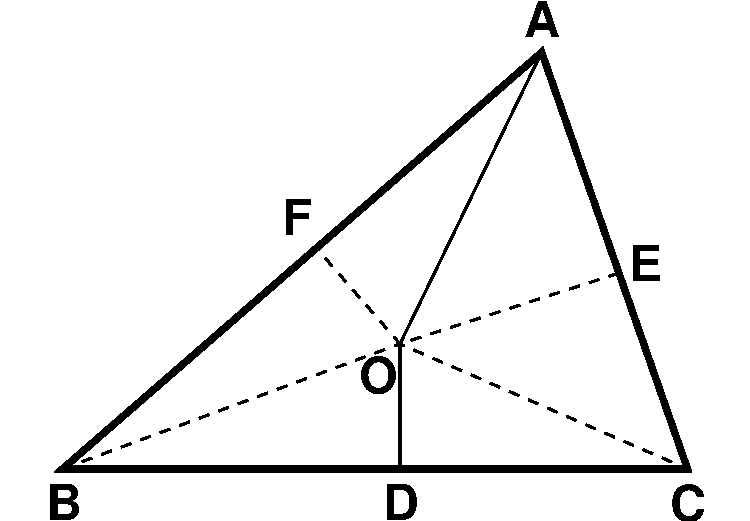
\includegraphics[width=6cm,viewport=0 5 360 245]{./images/illus061.pdf} % size graphic using BoundingBox
\else\includegraphics[width=6cm]{./images/illus061.eps}\fi
\end{wrapfigure}

Let us begin by taking the case
where $O$ is inside the triangle, in
which case $E$ falls on $AC$ and $F$ on
$AB$. %Corrected BC to AB to fix typo in original 

The triangles $AOF$ and $AOE$ are
equal, since the side $AO$ is common,
angle $OAF = \text{angle}$  $OAE$, and angle $OFA= \text{angle}$ $OEA$. Hence
$AF=AE$. Also, the triangles $BOF$ and $COE$ are equal. For
\PG----File: 062.png-----------------------------------------------------
since $OD$ bisects $BC$ at right angles, we have $OB=OC$; also,
since the triangles $AOF$ and $AOE$ are equal, we have
$OF=OE$; lastly, the angles at $F$ and $E$ are right angles.
Therefore, by Euc.~\textsc{i}.~47 and \textsc{i}.~8, the triangles $BOF$
and $COE$ are equal. Hence $FB=EC$.

Therefore $AF+FB=AE+EC$, that is, $AB=AC$.

The same demonstration will cover the case where $DO$ and
$AO$ meet at $D$, as also the case where they meet outside $BC$
but so near it that $E$ and $F$ fall on $AC$ and $AB$ and not on
$AC$ and $AB$ produced.

Next take the case where $DO$ and $AO$ meet outside the
triangle, and $E$ and $F$ fall on $AC$ and $AB$ produced. Draw
$OE$ perpendicular to $AC$ produced. Draw $OF$ perpendicular
to $AB$ produced. Join $OB$, $OC$.

\begin{figure*}[!hbt]
\centerline{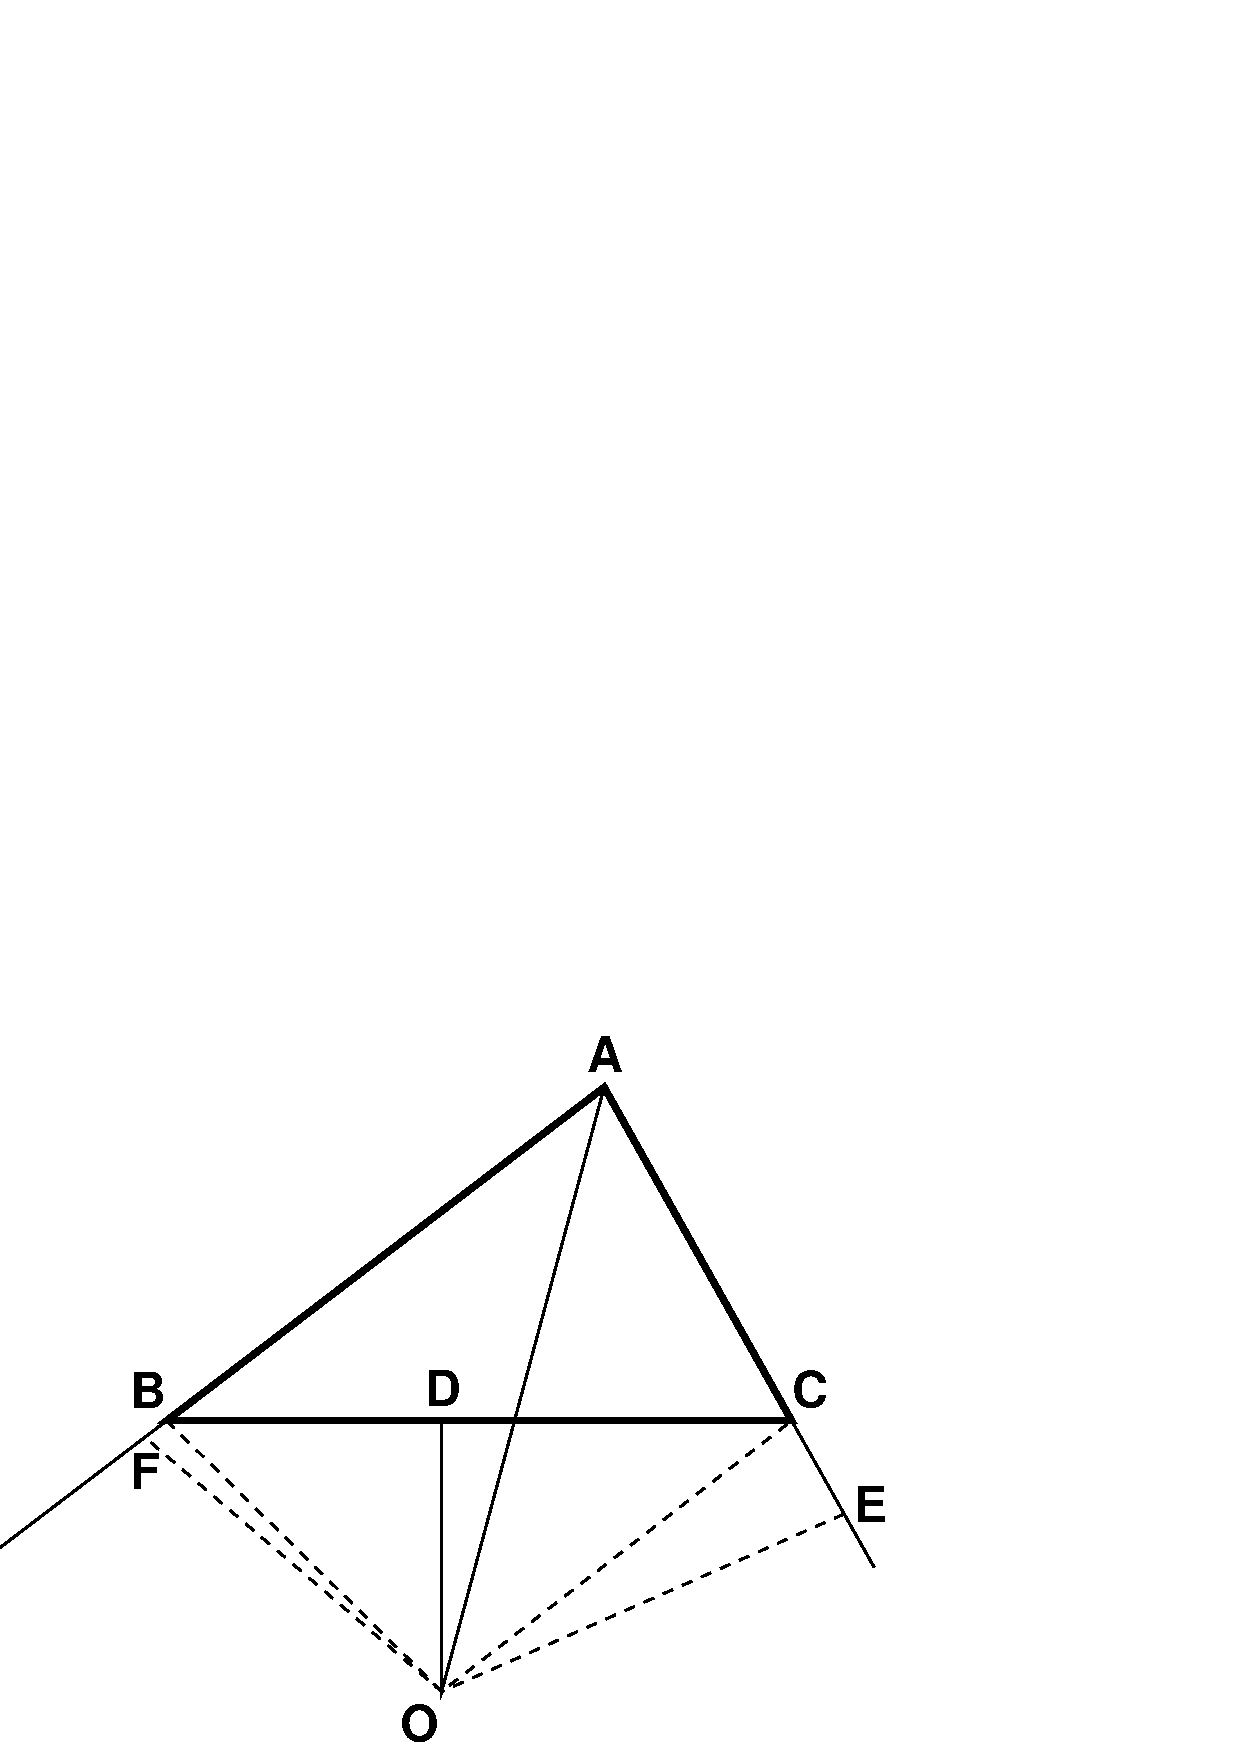
\includegraphics[width=\ifPaper.6\else.5\fi\textwidth]{./images/illus062}}
\end{figure*}

Following the same argument as before, from the equality
of the triangles $AOF$ and $AOE$, we obtain $AF=AE$; and,
from the equality of the triangles $BOF$ and $COE$, we obtain
$FB=EC$. Therefore $AF-FB=AE-EC$, that is, $AB=AC$.

Thus in all cases, whether or not $DO$ and $AO$ meet, and
whether they meet inside or outside the triangle, we have
$AB = AC$: and therefore every triangle is isosceles, a result
which is impossible.
% The explanation of the fallacy is that in fact there is a case not covered:
% F falls between A and B but E falls outside A and C (or vice versa), so
% AB = AF + FB but AC = AE - CE = AF - FB

\subsection*{Fourth Fallacy} I am indebted to Captain Turton\index
{Turton, W.H.} for the following ingenious fallacy; it appeared for the first
time in the third edition of this work.

On the hypothenuse, $BC$, of an isosceles right-angled
\PG----File: 063.png-----------------------------------------------------
triangle, $DBC$, describe an equilateral triangle $ABC$, the
vertex $A$ being on the same side of the base as $D$ is. On $CA$
take a point $H$ so that $CH = CD$. Bisect $BD$ in $K$. Join $HK$
and let it cut $CB$ (produced) in $L$. Join $DL$. Bisect $DL$ at
$M$, and through $M$ draw $MO$ perpendicular to $DL$. Bisect
$HL$ at $N$, and through $N$ draw $NO$ perpendicular to $HL$.
Since $DL$ and $HL$ intersect, therefore $MO$ and $NO$ will also
intersect; moreover, since $BDC$ is a right angle, $MO$ and $NO$
both slope away from $DC$ and therefore they will meet on the
side of $DL$ remote from $A$. Join $OC$, $OD$, $OH$, $OL$.

The triangles $OMD$ and $OML$ are equal, hence $OD = OL$.
Similarly the triangles $ONL$ and $ONH$ are equal, hence
$OL = OH$. Therefore $OD = OH$. Now in the triangles $OCD$
and $OCH$, we have $OD= OH$, $CD = CH$ (by construction), and
$OC$ common, hence (by Euc.~\textsc{i}.~8) the angle $OCD$ is equal to
the angle $OCH$, which is absurd.

\subsection*{Fifth Fallacy\protect\footnote
{\textit{Mathesis}, October, 1893, series~2, vol.~\textsc{iii}, p.~224.}}
\emph{To prove that, if two opposite sides of a
quadrilateral are equal, the other two sides must be parallel.}
Let $ABCD$ be a quadrilateral such that $AB$ is equal to $DC$.
Bisect $AD$ in $M$, and through $M$ draw $MO$ at right angles to
$AD$. Bisect $BC$ in $N$, and draw $NO$ at right angles to $BC$.

If $MO$ and $NO$ are parallel, then $AD$ and $BC$ (which are
at right angles to them) are also parallel.

If $MO$ and $NO$ are not parallel, let them meet in $O$; then
$O$ must be either inside the quadrilateral as in the left-hand
\begin{figure*}[!hbt]
\centering
\ifPaper\else\hspace*{\fill}\fi
\begin{minipage}{\ifPaper0.45\textwidth\else0.33\textwidth\fi}
\centerline{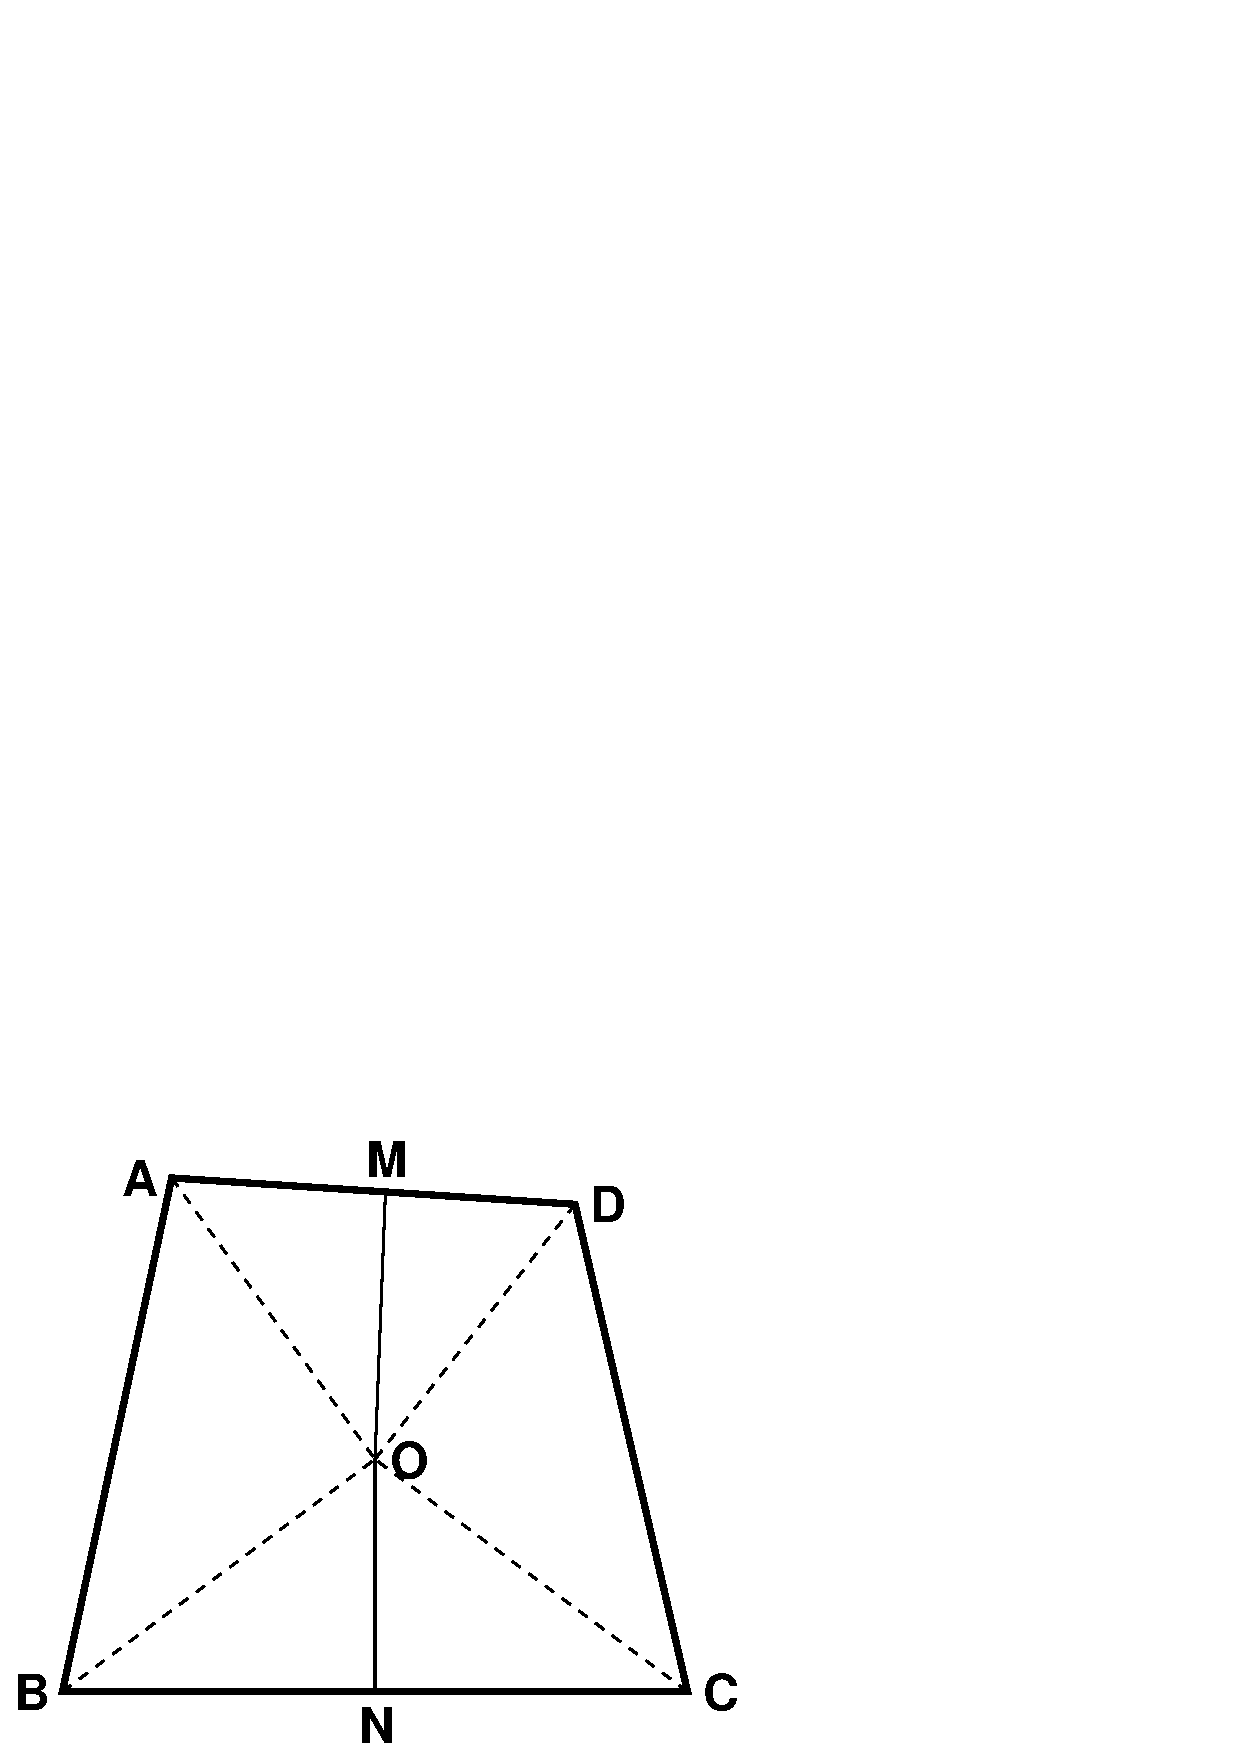
\includegraphics[width=\textwidth]{./images/illus063a}}
\end{minipage}
\hfill
\begin{minipage}{\ifPaper0.45\textwidth\else0.33\textwidth\fi}
\centerline{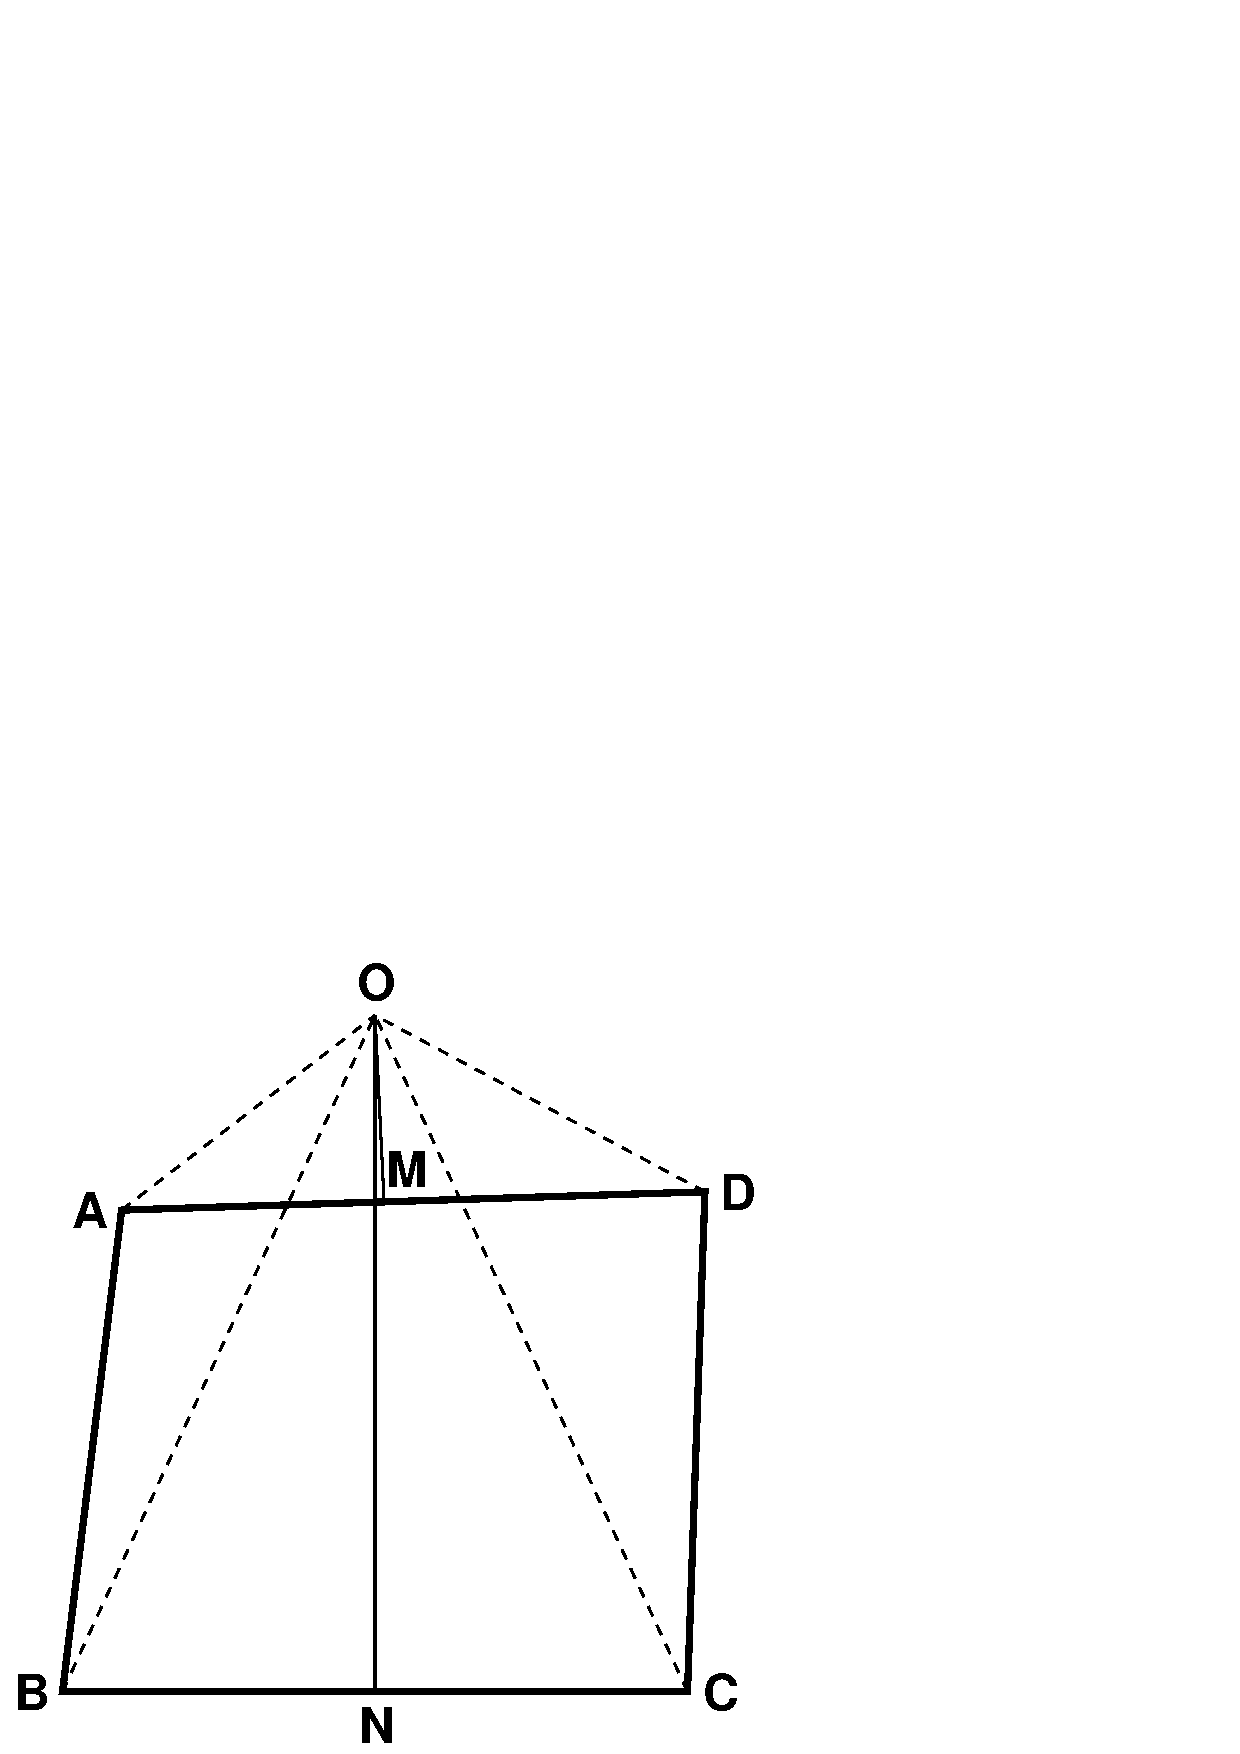
\includegraphics[width=\textwidth]{./images/illus063b}}
\end{minipage}
\ifPaper\else\hspace*{\fill}\fi
\end{figure*}
diagram or outside the quadrilateral as in the right-hand
diagram. Join $OA$, $OB$, $OC$, $OD$.

\PG----File: 064.png-------------------------------------------------------
Since $OM$ bisects $AD$ and is perpendicular to it, we have
$OA =\allowbreak OD$, and the angle $OAM$ equal to the angle $ODM$.
Similarly $OB = OC$, and the angle $OBN$ equal to the angle
$OCN$. Also by hypothesis $AB = DC$, hence, by Euc.~\textsc{i}.~8, the
triangles $OAB$ and $ODC$ are equal in all respects, and therefore
the angle $AOB$ is equal to the angle $DOC$.

Hence in the left-hand diagram the sum of the angles
$AOM$, $AOB$ is equal to the sum of the angles $DOM$, $DOC$;
and in the right-hand diagram the difference of the angles
$AOM$, $AOB$ is equal to the difference of the angles $DOM$, $DOC$;
and therefore in both cases the angle $MOB$ is equal to the
angle $MOC$, \IE\ $OM$ (or $OM$ produced) bisects the angle $BOC$.
But the angle $NOB$ is equal to the angle $NOC$, \IE\ $ON$ bisects
the angle $BOC$; hence $OM$ and $ON$ coincide in direction.
Therefore $AD$ and $BC$, which are perpendicular to this direction,
must be parallel. This result is not universally true,
and the above demonstration contains a flaw.

\subsection*{Sixth Fallacy} The following argument is taken from a
text-book on electricity, published in 1889 by two distinguished
mathematicians, in which it was presented as valid. A given
vector $OP$ of length $l$ can be resolved in an infinite number
of ways into two vectors $OM$, $MP$, of lengths $l'$, $l''$, and we
can make $l'/l''$ have any value we please from nothing to
infinity. Suppose that the system is referred to rectangular
axes $Ox$, $Oy$; and that $OP$, $OM$, $MP$ make respectively angles
$\theta$, $\theta'$, $\theta''$ with $Ox$. Hence, by projection on $Oy$
and on $Ox$, we have
\begin{LRalign}
&l\sin\theta &= l'\sin\theta' + l''\sin\theta''\,,\\
&l\cos\theta &= l'\cos\theta' + l''\cos\theta''\,.\\
Therefore
&\tan\theta &= \frac{n\sin\theta' + \sin\theta''}{n\cos\theta' +
 \cos\theta''}\,,\\
\end{LRalign}
where $n = l'/l''$. This result is true whatever be the value of $n$.
But $n$ may have any value (\Eg~$n = \infty$, or $n = 0$), hence
$\tan\theta = \tan\theta' = \tan\theta''$, which obviously is impossible.

\subsection*{Seventh Fallacy} Here is a fallacious investigation, to
\PG----File: 065.png------------------------------------------------------
which Mr~Chartres\index{Chartres, R.} first called my attention, of the value
of $\pi$: it is founded on well-known quadratures. The area of the
semi-ellipse bounded by the minor axis is (in the usual notation)
equal to $\frac{1}{2}\pi ab$. If the centre is moved off to an
indefinitely great distance along the major axis, the ellipse
degenerates into a parabola, and therefore in this particular
limiting position the area is equal to two-thirds of the circumscribing
rectangle. But the first result is true whatever be
the dimensions of the curve.
\begin{align*}
\Therefore \tfrac{1}{2}\pi ab & = \tfrac{2}{3}a \times 2b,\\
\Therefore \pi & = 8/3,
\end{align*}
a result which is obviously untrue%
\index{FallaciesGeom@\nobreak--- \textsc{Geometrical}|)}%
\index{Geometrical Fallacies@\textsc{Geometrical Fallacies}|)}.

\section{Geometrical Paradoxes} To the above examples I may
add the following questions, which, though not exactly
fallacious, lead to results which at a hasty glance appear
impossible.

\subsection*{First Paradox} The first is a problem, sent to me by
Mr~Renton\index{Renton}, to rotate a plane lamina (say, for instance, a
sheet of paper) through four right angles so that the effect is
equivalent to turning it through only one right angle.

If it is desired that the effect shall be equivalent to turning
it through a right angle about a point $O$, the solution is as
follows. Describe on the lamina a square $OABC$. Rotate
the lamina successively through two right angles about the
diagonal $OB$ as axis and through two right angles about the
side $OA$ as axis, and the required result will be attained.

\subsection*{Second Paradox} As in arithmetic, so in geometry, the
theory of probability\index{Probabilities, Fallacies in} lends itself to
numerous paradoxes.
Here is a very simple illustration. A stick is broken at
random into three pieces. It is possible to put them together
into the shape of a triangle provided the length of the
longest piece is less than the sum of the other two pieces
(\textit{cf.} Euc.~\textsc{i}.~20), that is, provided the length of the
longest piece is less than half the length of the stick. But the
probability that a fragment of a stick shall be half the
\PG----File: 066.png---------------------------------------------------------
original length of the stick is $\frac{1}{2}$. Hence the probability that
a triangle can be constructed out of the three pieces into
which the stick is broken would appear to be $\frac{1}{2}$. This is not
true, for actually the probability is $\frac{1}{4}$.

\subsection*{Third Paradox} The following example illustrates how
easily the eye may be deceived in demonstrations obtained by
actually dissecting\index{Dissection, Proofs by|(} the figures and
re-arranging the parts. In
fact proofs by superposition should be regarded with considerable
distrust unless they are supplemented by mathematical
reasoning. The well-known proofs of the propositions
Euclid~\textsc{i}.~32\index{Eucy@Euclid \textsc{i}. 32}
and Euclid~\textsc{i}.~47\index{Eucz@Euclid \textsc{i}. 47} can be so
supplemented and
are valid. On the other hand, as an illustration of how
deceptive a non-mathematical proof may be, I here mention
the familiar paradox that a square of paper, subdivided like
a chessboard into $64$ small squares, can be cut into four pieces
\begin{figure*}[!hbt]
\centerline{\ifpdf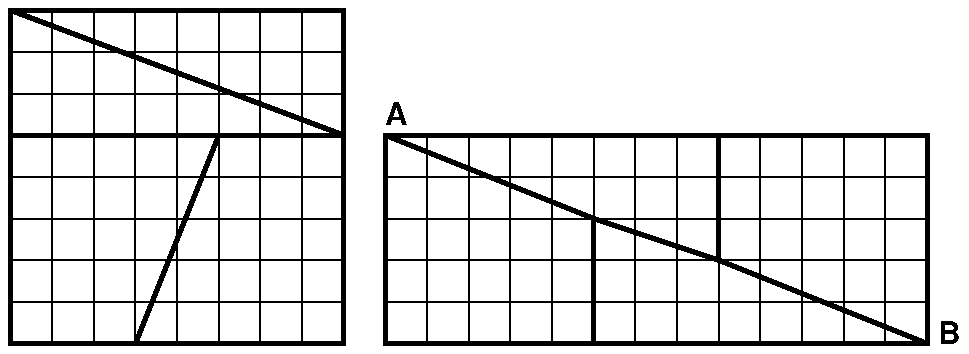
\includegraphics[width=.9\textwidth,viewport=0 0 450 170]{./images/illus066.pdf} % size graphic using BoundingBox
\else\includegraphics[width=.9\textwidth]{./images/illus066.eps}\fi\DPlabel{illus066}}
\end{figure*}
which being put together form a figure containing $65$\index
{Sixty-five Puzzle} such small squares\footnote
{I do not know who discovered this paradox. It is given in various
modern books, but I cannot find an earlier reference to it than one by
Prof.\ G.H.~Darwin\index{Darwin, G.H.}, \textit{Messenger of Mathematics},
1877, vol.~\textsc{vi}, p.~87.}.
This is effected by cutting the original square
into four pieces in the manner indicated by the thick lines in
the \vhyperlink{illus066}{first figure}. If these four pieces are put
together in the shape of a rectangle in the way shown in the
\vhyperlink{illus066}{second figure}
it will appear as if this rectangle contains $65$ of the small
squares.

\PG----File: 067.png------------------------------------------------------
This phenomenon, which in my experience non-mathematicians find
perplexing, is due to the fact that the edges
of the four pieces of paper, which in the second figure lie along
the diagonal $AB$, do not coincide exactly in direction. In
reality they include a small lozenge or diamond-shaped figure,
whose area is equal to that of one of the $64$ small squares in
the original square, but whose length $AB$ is much greater than
its breadth. The diagrams show that the angle between the
two sides of this lozenge which meet at $A$ is
$\tan^{-1}\frac{2}{5} - \tan^{-1}\frac{3}{8}$,
that is, is $\tan^{-1}\frac{1}{46}$, which is less than
$1\frac{1}{4}^{\circ}$. To enable the
eye to distinguish so small an angle as this the dividing lines
in the first figure would have to be cut with extreme accuracy
and the pieces placed together with great care.

The paradox depends upon the relation $5 \times 13 - 8^2 = 1$. Similar
results can be obtained from the formulae $13 \times 34 - 21^2 = 1$,
$34 \times 89 - 55^2 = 1$,\textellipsis; or from the formulae
$5^2 - 3 \times 8 = 1$,
$13^2 - 8 \times 21 = 1$, $34^2 - 21 \times 55 = 1$,\textellipsis.
These numbers are obtained by finding convergents to the continued fraction
\[
1 + \frac{1}{1} \genfrac{}{}{0pt}{}{}{+} % \underset{+}{} gives a too-small +
      \frac{1}{1} \genfrac{}{}{0pt}{}{}{+}
      \frac{1}{1} \genfrac{}{}{0pt}{}{}{+} \dotsb\, .
\]

A similar paradox for a square of $17$ cells, by which it was
shown that $289$ was equal to $288$, was alluded to by Ozanam\footnote
{Ozanam\index{Ozanam@Ozanam's \textit{Récréations}}, 1803 edition,
vol.~\textsc{i}, p.~299.}
who gave also the diagram for dividing a rectangle of $11$ by
$3$ into two rectangles whose dimensions appear to be $5$ by $4$
and $7$ by $2$.

\subsection*{Turton's Seventy-Seven Puzzle} A far better dissection
puzzle was invented by Captain Turton\index{Turton, W.H.}\index
{Seventy-seven Puzzle}. In this a piece of
cardboard, $11$ inches by $7$ inches, subdivided into $77$ small
equal squares, each $1$ inch by $1$ inch, can be cut up and
re-arranged so as to give $78$ such equal squares, each $1$ inch
by $1$ inch, of which $77$ are arranged in a rectangle of the same
dimensions as the original rectangle from one side of which
projects a small additional square. The construction is ingenious,
\PG----File: 068.png------------------------------------------------------
but cannot be described without the use of a model.
The trick consists in utilizing the fact that cardboard has a
sensible thickness. Hence the edges of the cuts can be
bevelled, but in the model the bevelling is so slight as to be
imperceptible save on a very close scrutiny. The play thus
given in fitting the pieces together permits the apparent
production of an additional square\index{Dissection, Proofs by|)}.

\section[Colouring Maps][The Four-Colour Theorem.]{Colouring Maps}
I proceed next to mention the%
\index{Colouring@\textsc{Colouring Maps}|(}%
\index{Four-Colour Theorem|(}%
\index{Map@\textsc{Map Colour Theorem}|(}
geometrical proposition that \emph{not more than four colours are
necessary in order to colour a map of a country (divided into
districts) in such a way that no two contiguous districts shall
be of the same colour}. By contiguous districts are meant
districts having a common \emph{line} as part of their boundaries:
districts which touch only at points are not contiguous in this
sense.

The problem was mentioned by A.F.~Möbius\footnote
{\textit{Leipzig Transactions} (\textit{Math.-phys. Classe}), 1885,
vol.~\textsc{xxxvii}, pp.~1--6.} in his
Lectures in 1840, but it was not until Francis Guthrie\index
{Guthrie on colouring maps}\footnote
{\textit{Proceedings of the Royal Society of Edinburgh}, July~19, 1880,
vol.~\textsc{x}, p.~728.}
communicated it to De~Morgan\index{DeMorgan@De Morgan, A.} about 1850 that
attention was
generally called to it: it is said that the fact had been
familiar to practical map-makers for a long time previously.
Through De~Morgan the proposition became generally known;
and in 1878 Cayley\index{Cayley}\footnote
{\textit{Proceedings of the London Mathematical Society}, 1878,
vol.~\textsc{ix},
p.~148, and \textit{Proceedings of the Royal Geographical Society}, 1879,
N.S., vol.~\textsc{i}, p.~259.} recalled attention to it by stating that
he did not know of any rigorous proof of it.

Probably the following argument, though not a formal
demonstration, will satisfy the reader that the result is
true.

Let $A$, $B$, $C$ be three contiguous districts, and let $X$ be any
other district contiguous with all of them. Then $X$ must
\PG----File: 069.png------------------------------------------------------
lie either wholly outside the external boundary of the area
$ABC$ or wholly inside the internal boundary, that is, it must
occupy a position either like $X$ or like $X'$. In either case
every remaining occupied area in the figure is enclosed by
the boundaries of not more than three districts: hence there is
no possible way of drawing another area $Y$ which shall be
contiguous with $A$, $B$, $C$, and $X$. In other words, it is possible
to draw on a plane four areas which are contiguous, but it is
not possible to draw five such areas.

\begin{figure*}[!hbt]
\[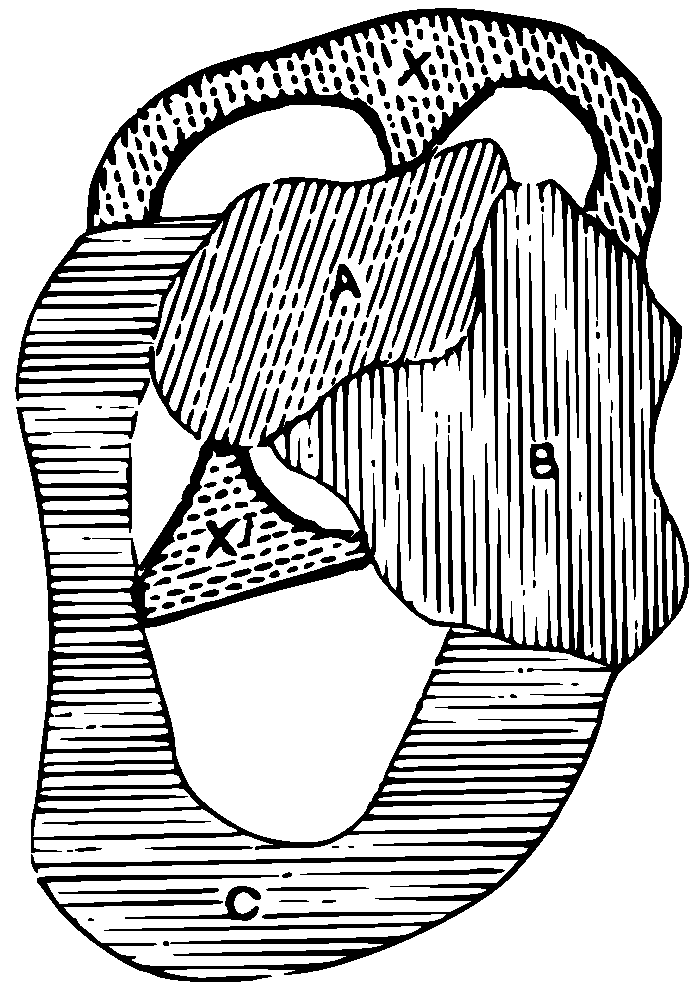
\includegraphics
[height=\ifPaper8cm\else.7\textheight\fi]{./images/illus069}\label{illus:069}\]
\end{figure*}

If $A$, $B$, $C$ are not contiguous, each with the other, or if $X$
is not contiguous with $A$, $B$, and $C$, it is not necessary to
colour them all differently, and thus the most unfavourable
case is that already treated. Moreover any of the above areas
may diminish to a point and finally disappear without affecting
the argument.

That we may require at least four colours is obvious from
the diagram \vpageref{illus:069}, %[*Note: originally "above diagram"]
since in that case the areas $A$, $B$, $C$, and $X$
would have to be coloured differently.

A proof of the proposition involves difficulties of a high
order, which as yet have baffled all attempts to surmount
them.

\PG----File: 070.png------------------------------------------------------
The argument by which the truth of the proposition
was formerly supposed to be demonstrated was given by
A.B.~Kempe\index{Kempe on Colouring Maps}\footnote
{He sent his first demonstration across the Atlantic to the \textit{American
Journal of Mathematics}, 1879, vol.~\textsc{ii}, pp.~193--200; but
subsequently he communicated it in simplified forms to the London Mathematical
Society, \textit{Transactions}, 1879, vol.~\textsc{x}, pp.~229--231, and to
\textit{Nature}, Feb.~26,
1880, vol.~\textsc{xxi}, pp.~399--400.} in 1879, but there is a flaw\footnote
{See articles by P.J.~Heawood\index{Heawood on Colouring Maps} in the \textit
{Quarterly Journal of Mathematics},
London, 1890, vol.~\textsc{xxiv}, pp.~332--338; and 1897, vol.~\textsc{xxxi},
pp.~270--285.}
in it.

In 1880, Tait\index{Tait} published a solution\footnote
{\textit{Proceedings of the Royal Society of Edinburgh}, July~19, 1880,
vol.~\textsc{x}, p.~729; and \textsc{Philosophical Magazine}, January, 1884,
series~5, vol.~\textsc{xvii}, p.~41.} depending on the
theorem that if a closed network of lines joining an even
number of points is such that three and only three lines meet
at each point then three colours are sufficient to colour the
lines in such a way that no two lines meeting at a point are of
the same colour; a closed network being supposed to exclude
the case where the lines can be divided into two groups
between which there is but one connecting line. His deduction
therefrom that four colours will suffice for a map was
given in the last edition of this work. The demonstration
appeared so straightforward that at first it was generally
accepted, but it would seem that it too involves a fallacy\footnote
{See J.~Peterson\index{Peterson on maps} of Copenhagen, \textit
{L'Intermédiaire des mathématiciens},
vol.~\textsc{v}, 1898, pp.~225--227; and vol.~\textsc{vi}, 1899, pp.~36--38.}.
The proof however leads to the interesting corollary that four
colours may not suffice for a map drawn on a multiply-connected
surface such as an anchor ring.

Although a proof of the theorem is still wanting\Editorial
{Appel and Haken's controversial computer-assisted proof
appeared in 1977: \textit{Illinois Journal of Mathematics},
vol.~\textsc{xxi}, pp.~429--490 and 491--567.}, no one
has succeeded in constructing a plane map which requires
more than four tints to colour it, and there is no reason to
doubt the correctness of the statement that it is not necessary
to have more than four colours for any plane map. The
number of ways which such a map can be coloured with four
\PG----File: 071.png------------------------------------------------------
tints has been also considered\footnote
{See A.C.~Dixon\index{Dixon, A.C.}, \textit{Messenger of Mathematics},
Cambridge, 1902--3, vol.~\textsc{xxxii}, pp.~81--83.},
but the results are not
sufficiently interesting to require mention here%
\index{Colouring@\textsc{Colouring Maps}|)}%
\index{Four-Colour Theorem|)}%
\index{Map@\textsc{Map Colour Theorem}|)}.

\section[Physical Geography][Hills and Dales.]%
{Physical Configuration of a Country} As I have been
alluding to maps, I may here mention that the theory of%
\index{Geography@\textsc{Geography, Physical}|(}%
\index{Hills@\textsc{Hills and Dales}|(}%
\index{Physical@\textsc{Physical Geography}|(}
the representation of the physical configuration of a country
by means of lines drawn on a map was discussed, by Cayley\index{Cayley}
and Clerk Maxwell\index{Maxwell, J. Clerk}\footnote
{Cayley on `\textit{Contour and Slope Lines},' \textit{Philosophical
 Magazine},
London, October, 1859, series~4, vol.~\textsc{xviii}, pp.~264--268;
 \textit{Collected
Works}, vol.~\textsc{iv}, pp.~108--111. J.~Clerk Maxwell on `\textit{Hills
 and Dales},'
\textit{Philosophical Magazine}, December, 1870, series~4, vol.~\textsc{xl},
 pp.~421--427;
\textit{Collected Works}, vol.~\textsc{ii}, pp.~233--240.}.
They showed that a certain relation
exists between the number of hills, dales, passes,~\&c.\ which
can co-exist on the earth or on an island. I proceed to give a
summary of their nomenclature and conclusions.

All places whose heights above the mean sea level are
equal are on the same level. The locus of such points on a
map is indicated by a \emph{contour-line}\index{Contour-lines}. Roughly
speaking, an island is bounded by a contour-line. It is usual to draw the
successive contour-lines on a map so that the difference between
the heights of any two successive lines is the same, and thus
the closer the contour-lines the steeper is the slope, but the
heights are measured dynamically by the amount of work to
be done to go from one level to the other and not by linear
distances.

A contour-line in general will be a closed curve. This
curve may enclose a region of elevation: if two such regions
meet at a point, that point will be a crunode (\IE\ a real double
point) on the contour-line through it, and such a point is
called a \emph{pass}. The contour-line may enclose a region of depression:
if two such regions meet at a point, that point
will be a crunode on the contour-line through it, and such
a point is called a \emph{fork} or bar. As the heights of the corresponding
level surfaces become greater, the areas of the regions
\PG----File: 072.png------------------------------------------------------
of elevation become smaller, and at last become reduced to
points: these points are the \emph{summits} of the corresponding
mountains. Similarly as the level surface sinks the regions of
depression contract, and at last are reduced to points: these
points are the \emph{bottoms} (or immits) of the corresponding valleys.

Lines drawn so as to be everywhere at right angles to
the contour-lines are called \emph{lines of slope}\index{Lines of Slope}. If
we go up a line of slope generally we shall reach a summit, and if we go
down such a line generally we shall reach a bottom: we may
come however in particular cases either to a pass or to a fork.
Districts whose lines of slope run to the same summit are
\emph{hills}. Those whose lines of slope run to the same bottom are
\emph{dales}. A \emph{watershed} is the line of slope from a summit to a
pass or a fork, and it separates two dales. A \emph{watercourse} is
the line of slope from a pass or a fork to a bottom, and it
separates two hills.

If $n + 1$ regions of elevation or of depression meet at a
point, the point is a multiple point on the contour-line drawn
through it; such a point is called a pass or a fork of the
$n$th order, and must be counted as $n$ separate passes (or forks).
If one region of depression meets another in several places at
once, one of these must be taken as a fork and the rest as passes.

Having now a definite geographical terminology we can
apply geometrical propositions to the subject. Let $h$ be the
number of hills on the earth (or an island), then there will be
also $h$ summits; let $d$ be the number of dales, then there will
be also $d$ bottoms; let $p$ be the whole number of passes, $p_1$ that
of single passes, $p_2$ of double passes, and so on; let $f$ be the
whole number of forks, $f_1$ that of single forks, $f_2$ of double
forks, and so on; let $w$ be the number of watercourses, then
there will be also $w$ watersheds\index{Watersheds and Watercourses}. Hence,
by the theorems of Cauchy\index{Cauchy} and Euler\index{Euler},
\begin{LRalign}
&  h &=1 + p_1 + 2p_2 + \dotsb\,,   \\
&  d &=1 + f_1 + 2f_2 + \dotsb\,,   \\
and  &  w &=2(p_1 + f_1) + 3(p_2 + f_2)) + \dotsb\,.\\
\end{LRalign}

\PG----File: 073.png---------------------------------------------------------
The above results can be extended to the case of a multiply-connected
closed surface%
\index{Geography@\textsc{Geography, Physical}|)}%
\index{Hills@\textsc{Hills and Dales}|)}%
\index{Physical@\textsc{Physical Geography}|)}.

\section*{Games} Leaving now the question of formal geometrical
propositions, I proceed to enumerate a few games or puzzles\index
{PuzzlesGeom@\nobreak--- Geometrical|(}
which depend mainly on the relative position of things, but
I postpone to \hyperlink{chapter.4}{chapter~\textsc{iv}} the discussion
of such amusements
of this kind as necessitate any considerable use of arithmetic
or algebra. Some writers regard draughts, solitaire, chess
and such like games as subjects for geometrical treatment
in the same way as they treat dominoes\index{Dominoes}, backgammon, and
games with dice in connection with arithmetic: but these
discussions require too many artificial assumptions to correspond
with the games as actually played or to be interesting.

The amusements to which I refer are of a more trivial
description, and it is possible that a mathematician may like
to omit the remainder of the chapter. In some cases it is
difficult to say whether they should be classified as mainly
arithmetical or geometrical, but the point is of no importance.

\ssection{Statical Games of Position} Of the innumerable statical%
\index{Counters, Games with|(}%
\index{GamesStatic@\nobreak--- Statical|(}%
\index{Statical@\textsc{Statical Games}|(}
games involving geometry of position I shall mention only
three or four.

\subsection[Three-in-a-row. \texorpdfstring{\protect\quad Extension to $p$-in-a-row}{ Extension to p-in-a-row}]%
[Three-in-a-row.]{Three-in-a-row}
First, I may mention the game of three-in-a-row\index{Row, Counters in a|(}%
\index{Three-in-a-row@\textsc{Three-in-a-row}|(},
of which noughts and crosses\index{Noughts and Crosses}, one form of merrilees,
and go-bang are well-known examples. These games are
played on a board---generally in the form of a square containing
$n^2$ small squares or cells. The common practice is for
one player to place a white counter or piece or to make a cross
on each small square or cell which he occupies: his opponent
similarly uses black counters or pieces or makes a nought on
each square which he occupies. Whoever first gets three (or
any other assigned number) of his pieces in three adjacent cells
and in a straight line wins. The mathematical theory for a
board of $9$ cells has been worked out completely, and there is
no difficulty in extending it to one of $16$ cells: but the analysis
is lengthy and not particularly interesting. Most of these
\PG----File: 074.png---------------------------------------------------------
games were known to the ancients\footnote
{\ifPaper\stretchyspace\fi
Becq de~Fouquières\index{DeFouqui@De Fouquières}%
\index{Fouqu@Fouquières on Ancient Games}, \textit{Les jeux des anciens},
second edition, Paris, 1873, chap.~\textsc{xviii}.}, and it is for that
reason I mention them here.

\subsection*{Three-in-a-row. Extension} I may, however, add an
elegant but difficult extension which has not previously found
its way, so far as I am aware, into any book of mathematical
recreations. The problem is to place $n$ counters on a plane
so as to form as many rows as possible, each of which shall
contain three and only three counters\footnote
{\textit{Educational Times Reprints}, 1868, vol.~\textsc{viii}, p.~106;
\Ibid\ 1886, vol.~\textsc{xlv}, pp.~127--128.}.

It is easy to arrange the counters in a number of rows
equal to the integral part of $\frac{1}{8}(n-1)^2$. This can be effected by
the following construction. Let $P$ be any point on a cubic.
Let the tangent at $P$ cut the curve again in $Q$. Let the tangent
at $Q$ cut the curve in $A$. Let $PA$ cut the curve in $B$, $QB$ cut
it in $C$, $PC$ cut it in $D$, $QD$ cut it in $E$, and so on. Then the
counters must be placed at the points $P, Q, A, B,\dots$. Thus $9$
counters can be placed in 8 such rows; 10 counters in 10 rows;
15 counters in 24 rows; 81 counters in 800 rows; and so on.

If however the point $P$ is a pluperfect point of the $n$th order
on the cubic, then Sylvester\index{Sylvester} proved that the above
construction gives a number of rows equal to the integral part of
$\frac{1}{6}(n-1)(n-2)$. Thus 9 counters can be arranged in 9 rows,
which is a well-known and easy puzzle; 10 counters in 12 rows;
15 counters in 30 rows; and so on.

Even this however is an inferior limit and may be exceeded---for
instance, Sylvester stated that 9 counters can be
placed in 10 rows, each containing three counters; I do not
know how he placed them, but one way of so arranging them
is by putting them at points whose coordinates are $(2, 0)$, $(2, 2)$,
$(2, 4)$, $(4, 0)$, $(4, 2)$, $(4, 4)$, $(0, 0)$, $(3, 2)$, $(6, 4)$; another
way is by putting them at the points $(0, 0)$, $(0, 2)$, $(0, 4)$, $(2, 1)$,
$(2, 2)$, $(2, 3)$, $(4, 0)$, $(4, 2)$, $(4, 4)$; more generally, the angular
points of a regular hexagon and the three points of intersection
\PG----File: 075.png---------------------------------------------------------
of opposite sides form such a group, and therefore any
projection of that figure will give a solution.

Thus at present it is not possible to say what is the maximum
number of rows of three which can be formed from $n$
counters placed on a plane.

\markright{$p$-in-a-row}
\subsection*{Extension to $p$-in-a-row} The problem mentioned above at
once suggests the extension of placing $n$ counters so as to form
as many rows as possible, each of which shall contain $p$ and
only $p$ counters. Such problems can be often solved immediately
by placing at infinity the points of intersection of
some of the lines, and (if it is so desired) subsequently projecting
the diagram thus formed so as to bring these points to
a finite distance. One instance of such a solution is given
above.

As easy examples I may give the arrangement of $16$
counters in $15$ rows\footnoteT{`13' corrected to '15' as per errata sheet}, each
containing $4$ counters; and the
arrangement of $19$ counters in $10$ rows, each containing $5$
counters. A solution of the second of these problems can be
obtained by placing counters at the $19$ points of intersection of
the $10$ lines $x=\pm a$, $x=\pm b$, $y=\pm a$, $y=\pm b$, $y=\pm x$: of
these points two are at infinity. The first problem I leave to the
ingenuity of my readers\index{Counters, Games with|)}%
\index{Row, Counters in a|)}%
\index{Three-in-a-row@\textsc{Three-in-a-row}|)}.

\subsection[Tesselation. \texorpdfstring{\protect\quad}{} Cross-Fours]%
[Tesselation. Cross-Fours.]{Tesselation}
Another of these statical recreations is known
as tesselation\index{Tesselation|(} and consists in the formation of
geometrical
designs or mosaics\index{Mosaic Pavements} by means of tesselated tiles.

To those who have never looked into the matter it may be
surprising that patterns formed by the use of square tiles (of
which one-half bounded by a diagonal is white and the other
half black) should be subject to mathematical analysis. In
view of the discussion of this subject by Montucla\index{Montucla}\footnote
{See Ozanam\index{Ozanam@Ozanam's \textit{Récréations}}, 1803 edition,
 vol.~\textsc{i}, p.~100; 1840 edition, p.~46.}, Lucas\index
{Lucas, E.}\footnote
{Lucas, \textit{Récréations Mathématiques}, Paris, 1882--3,
 vol.~\textsc{ii}, part~4:
hereafter I shall refer to this work by the name of the author.},
and other writers it would be hard to refuse to call the
formation of such patterns a mathematical amusement, but
the treatment is (perhaps necessarily) somewhat empirical,
\PG----File: 076.png---------------------------------------------------------
and though there are some interesting puzzles of this kind, I
do not propose to describe them here.

Sylvester\index{Sylvester}\footnote
{\EG\ see the \textit{Educational Times Reprints}, London, 1868,
 vol.~\textsc{x},
pp.~74--76, 112: see also vol.~\textsc{xlv}, p.~127; vol.~\textsc{lvi},
 pp.~97--99.}
proposed a modified tesselation problem which
consists in forming anallagmatic squares\index{Anallagmatic Squares}, that is,
squares such that in every row and every column the number of changes of
colour or the number of permanences is constant, the tiles used
being square white tiles and square black tiles.

If more than two colours are used, the problems become
increasingly difficult. As a simple instance of this class of
problems I may mention one, sent to me by a correspondent
who termed it \emph{Cross-Fours}\index{Cross-fours}, wherein sixteen square
counters are used, the upper half of each being yellow, red, pink,
or blue, and the lower half being gold, green, black, or white,
no two counters being coloured alike. Such counters can be
arranged in the form of a square so that in each vertical,
horizontal, and diagonal line there shall be 8 colours and no
more: they can be also arranged so that in each of these ten
lines there shall be 6 colours and no more, or 5 colours and no
more, or 4 colours and no more. Puzzles of this kind are but
little known; they are however not uninstructive\index{Tesselation|)}.

\subsection{Colour-Cube Problem} As an example of a recreation%
\index{Colour-cube@\textsc{Colour-cube Problem}|(}
\index{Cubes, Coloured|(}
analogous to tesselation I will mention the colour-cube problem;
I select this partly because it is one of the most difficult
of such puzzles, but chiefly because it has been subjected\footnote
{By Major MacMahon\index{MacMahon}; an abstract of his paper, read before the
London Mathematical Society on Feb.~9, 1893, was given in \textit{Nature},
Feb.~23, 1893, vol.~\textsc{xlvii}, p.~406.} to
mathematical analysis.

Stripped of mathematical technicalities the problem may
be enunciated as follows. A cube has six faces, and if six
colours are chosen we can paint each face with a different
colour. By permuting the order of the colours we can obtain
thirty such cubes, no two of which are coloured alike. Take
any one of these cubes, $K$, then it is desired to select eight
\PG----File: 077.png--------------------------------------------------
out of the remaining twenty-nine cubes, such that they can be
arranged in the form of a cube (whose linear dimensions are
double those of any of the separate cubes) coloured like the
cube $K$, and placed so that where any two cubes touch each
other the faces in contact are coloured alike.

Only one collection of eight cubes can be found to satisfy
these conditions. To pick out these eight cubes empirically
would be out of the question, but the mathematical analysis
enables us to select them by the following rule. Take any
face of the cube $K$: it has four angles, and at each angle
three colours meet. By permuting the colours cyclically we
can obtain from each angle two other cubes, and the eight
cubes so obtained are those required.

For instance suppose that the six colours are indicated
by the letters $a$, $b$, $c$, $d$, $e$, $f$. Let the cube $K$ be put on a
table, and to fix our ideas suppose that the face coloured $f$ is
at the bottom, the face coloured $a$ is at the top, and the faces
coloured $b$, $c$, $d$, and $e$ front respectively the east, north, west,
and south points of the compass. I may denote such an
arrangement by \Cube(f; a; b, c, d, e). One cyclical permutation
of the colours which meet at the north-east corner of the
top face gives the cube \Cube(f; c; a, b, d, e), and a second cyclical
permutation gives the cube \Cube(f; b; c, a, d, e). Similarly
cyclical permutations of the colours which meet at the north-west
corner of the top face of $K$ give the cubes \Cube(f; d; b, a, c, e)
and \Cube(f; c; b, d, a, e). Similarly from the top south-west
corner of $K$ we get the cubes \Cube(f; e; b, c, a, d) and
\Cube(f; d; b, c, e, a): and from the top south-east corner we get % note colon is clear in scan
the cubes \Cube(f; e; a, c, d, b) and \Cube(f; b; e, c, d, a).

The eight cubes being thus determined it is not difficult to
arrange them in the form of a cube coloured similarly to $K$,
and subject to the condition that faces in contact are coloured
alike; in fact they can be arranged in two ways to satisfy
these conditions. One such way, taking the cubes in the
numerical order given above, is to put the cubes $3$, $6$, $8$, and $2$
at the SE, NE, NW, and SW corners of the bottom face; of
\PG----File: 078.png--------------------------------------------------
course each placed with the colour $f$ at the bottom, while $3$
and $6$ have the colour $b$ to the east, and $2$ and $8$ have the
colour $d$ to the west: the cubes $7$, $1$, $4$, and $5$ will then form
the SE, NE, NW, and SW corners of the top face; of course
each placed with the colour $a$ at the top, while $7$ and $1$ have
the colour $b$ to the east, and $5$ and $4$ have the colour $d$ to the
west. If however $K$ is not given, then, without the aid of
mathematical analysis, it is a difficult puzzle to arrange the
eight cubes in the form of a cube coloured similarly to one of
the other twenty-two cubes and subject to the condition that
faces in contact are coloured alike%
\index{Colour-cube@\textsc{Colour-cube Problem}|)}%
\index{Cubes, Coloured|)}%
\index{GamesStatic@\nobreak--- Statical|)}%
\index{Statical@\textsc{Statical Games}|)}.

It is easy to make similar puzzles in two dimensions which
are fairly difficult; it is somewhat surprising that none are to
be bought, but I have never seen any except those that I have
made myself.

\ssection[Dynamical Games of Position][Dynamical Geometrical Games.]%
{Dynamical Games of Position} Games which are played
by moving pieces on boards of various shapes%
\index{Dynamical@\textsc{Dynamical Games}|(}%
\index{Games@\textsc{Games}, Dynamical|(}---such as merrilees,
fox and geese, solitaire, backgammon, draughts, and
chess---present more interest. In general, however, they permit
of so many movements of the pieces that any mathematical
analysis of them becomes too intricate to follow out completely.
Probably this is obvious, but it may emphasize the impossibility
of discussing such games effectively if I add that it has
been shown that in a game of chess there may be as many
as $197299$ ways of playing the first four moves, and nearly
$72000$ different positions at the end of the first four moves
(two on each side), of which $16556$ arise when the players
move pawns only\footnote
{\textit{L'Intermédiaire des mathématiciens}, Paris, December, 1903,
 vol.~\textsc{x},
pp.~305--308: also \textit{Royal Engineers Journal}, London, August--November,
1889; or \textit{British Association Transactions}, 1890, p.~745.}.

Games in which the possible movements are very limited
may be susceptible of mathematical treatment. One or two
of these are given in the next chapter: here I shall confine
myself mainly to puzzles and simple amusements.

\subsection{Shunting Problems} The first I will mention is a little
\PG----File: 079.png--------------------------------------------------
puzzle which I bought some years ago and which was described
as the ``Great Northern puzzle%
\index{Railway Puzzles (shunting)|(}%
\index{Shunting@\textsc{Shunting Problems}|(}.'' It is typical of a good many
problems connected with the shunting of trains, and though it
rests on a most improbable hypothesis, I give it as a specimen
of its kind.

\begin{figure*}[!hbt]
\centerline{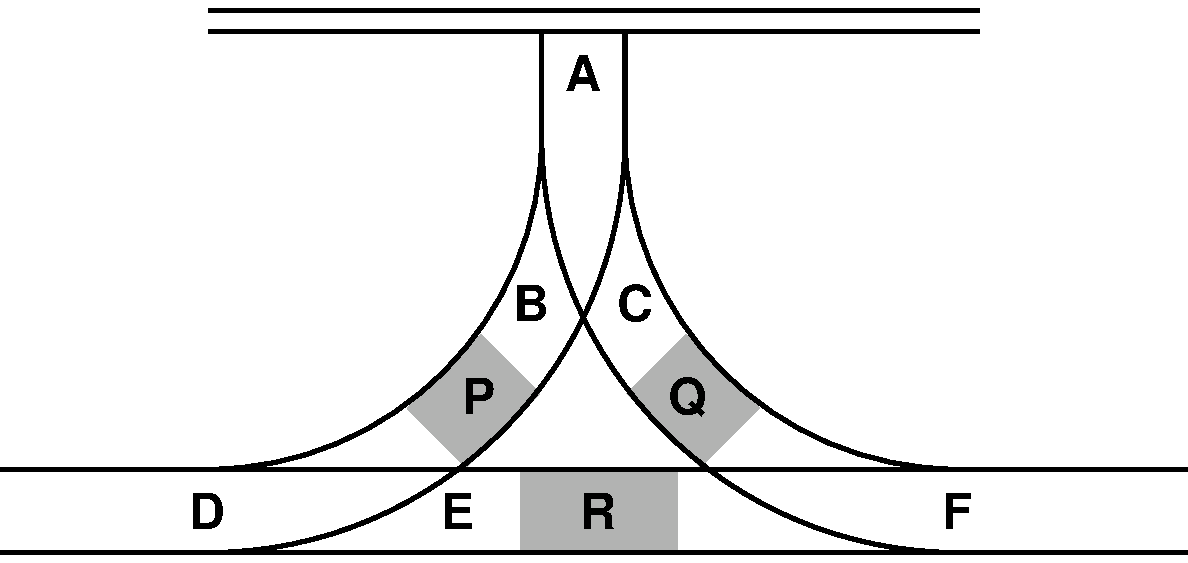
\includegraphics
[width=\ifPaper.8\else.6\fi\textwidth]{./images/illus079}}
\end{figure*}

The puzzle shows a railway, $DEF$, with two sidings, $DBA$
and $FCA$, connected at $A$. The portion of the rails at $A$
which is common to the two sidings is long enough to permit
of a single wagon, like $P$ or $Q$, running in or out of it; but
is too short to contain the whole of an engine, like $R$. Hence,
if an engine runs up one siding, such as $DBA$, it must come
back the same way.

Initially a small block of wood, $P$, coloured to represent a
wagon, is placed at $B$; a similar block, $Q$, is placed at $C$; and
a longer block of wood, $R$, representing an engine, is placed at
$E$. The problem is to use the engine $R$ to interchange the
wagons $P$ and $Q$, without allowing any flying shunts.

This is effected thus. (i)~$R$ pushes $P$ into $A$. (ii)~$R$ returns,
pushes $Q$ up to $P$ in $A$, couples $Q$ to $P$, draws them both out
to $F$, and then pushes them to $E$. (iii)~$P$ is now uncoupled,
$R$ takes $Q$ back to $A$, and leaves it there. (iv)~$R$ returns to $P$,
pulls $P$ back to $C$, and leaves it there. (v)~$R$ running successively
through $F$, $D$, $B$ comes to $A$, draws $Q$ out, and leaves
it at $B$.

A somewhat similar puzzle, on sale in the streets in 1905,
is made as follows. A loop-line $BGE$ connects two points $B$
and $E$ on a railway track $AF$, which is supposed blocked at
both ends, as shown in the diagram. In the model, the track
\PG----File: 080.png--------------------------------------------------
$AF$ is 9 inches long, $AB = EF = 1\frac{5}{6}$ inches, and $AH = FK = BC
= DE = \frac{1}{4}$ inch. On the track and loop are eight wagons,
\begin{figure*}[!hbt]
\centerline{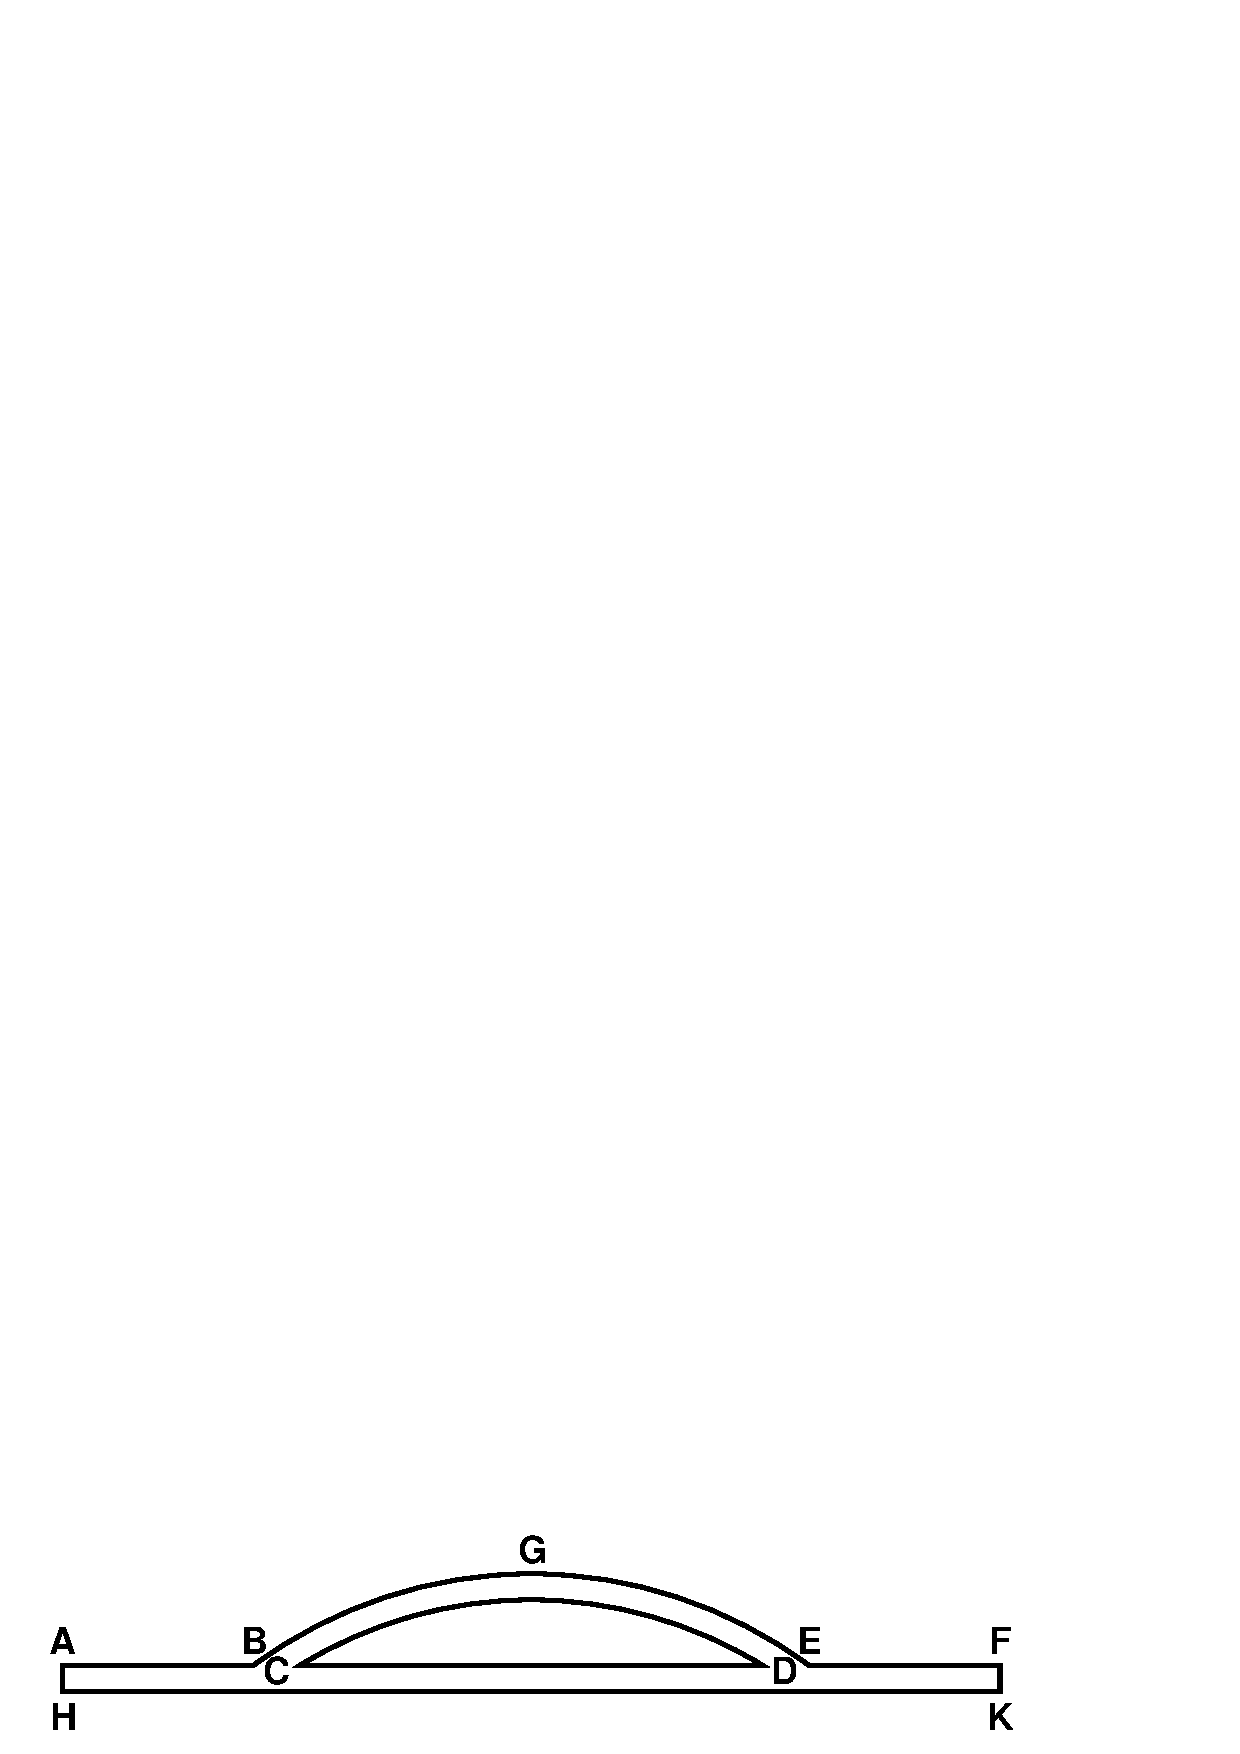
\includegraphics
[width=\ifPaper.9\else.8\fi\textwidth]{./images/illus080}}
\end{figure*}
numbered successively $1$ to $8$, each one inch long and one-quarter
of an inch broad, and an engine of the same dimensions.
Originally the wagons are on the track from $A$ to $F$
and in the order $1$, $2$, $3$, $4$, $5$, $6$, $7$, $8$, and the engine is on
the loop. The construction and the initial arrangement ensure that
at any one time there cannot be more than eight vehicles on
the track. Also if eight vehicles are on it only the penultimate
vehicle at either end can be moved on to the loop, but if less than
eight are on the track then the last two vehicles at either end
can be moved on to the loop. If the points at each end of the loop-line
are clear, it will hold four, but not more than four, vehicles.
The object is to reverse the order of the wagons on the track,
so that from $A$ to $F$ they will be numbered successively $8$ to $1$;
and to do this by means which will involve as few transferences
of the engine or a wagon to or from the loop as is possible.

Other shunting problems are not uncommon, but these two
examples will suffice%
\index{Railway Puzzles (shunting)|)}%
\index{Shunting@\textsc{Shunting Problems}|)}.

\subsection{Ferry-Boat Problems} Everybody is familiar with the story\index
{Ferry@\textsc{Ferry-boat Problems}|(}
of the showman who was travelling with a wolf, a goat, and a
basket of cabbages; and for obvious reasons was unable to leave
the wolf alone with the goat, or the goat alone with the cabbages.
The only means of transporting them across a river was a boat
so small that he could take in it only one of them at a time.
The problem is to show how the passage could be effected\footnote
{Ozanam\index{Ozanam@Ozanam's \textit{Récréations}}, 1803 edition,
 vol.~\textsc{i}, p.~171; 1840 edition, p.~77.}.

A similar problem, given by Alcuin\index{Alcuin}, Tartaglia\index
{Tartaglia}, and others, is as follows\footnote
{Bachet\index{Bachet@Bachet's \textit{Problèmes}}, Appendix,
 problem~\textsc{iv}, p.~212.}.
Three beautiful ladies have for husbands three
men, who are as jealous as they are young, handsome, and
\PG----File: 081.png--------------------------------------------------
gallant. The party are travelling, and find on the bank of
a river, over which they have to pass, a small boat which can
hold no more than two persons. How can they pass, it being
agreed that, in order to avoid scandal, no woman shall be left
in the society of a man unless her husband is present?

The method of transportation to be used in the above cases
is obvious, and can be illustrated practically by using six court
cards\index{Cards, Problems with} out of a pack. Another problem similar to
 the one last
mentioned is the case of $n$ married couples who have to cross
a river by means of a boat which can be rowed by one person
and will carry $n - 1$ people, but not more, with the condition
that no woman is to be in the society of a man unless her
husband is present. Alcuin's problem is the case of $n = 3$.
Let $y$ denote the number of passages from one bank to the
other which will be necessary. Then it has been shown that
if $n = 3$, $y = 11$; if $n = 4$, $y = 9$; and if $n > 4$, $y = 7$;
the demonstration presents no difficulty.

The following analogous problem is due to the late Prof.\
Lucas\index{Lucas, E.}\footnote
{Lucas, vol.~\textsc{i}, pp.~15--18, 237--238.}.
To find the smallest number $x$ of persons that a boat
must be able to carry in order that $n$ married couples may by
its aid cross a river in such a manner that no woman shall
remain in the company of any man unless her husband is
present; it being assumed that the boat can be rowed by one
person only. Also to find the least number of passages, say $y$,
from one bank to the other which will be required. M.~Delannoy\index{Delannoy}
has shown that if $n = 2$, then $x = 2$, and $y = 5$. If $n = 3$, then
$x = 2$, and $y = 11$. If $n = 4$, then $x = 3$, and $y = 9$. If $n = 5$, then
$x = 3$, and $y = 11$. And finally if $n > 5$, then $x = 4$, and $y = 2n - 1$.

M.~De~Fonteney\index{DeFont@De Fonteney on Ferry Problem}\index
{Fonteney on Ferry Problem} has remarked that, if there was an island
in the middle of the river, the passage might be always effected
by the aid of a boat which could carry only two persons. If there
are only two or only three couples the island is unnecessary,
and the case is covered by the preceding method. If $n > 3$
then the least number of passages from land to land which will
be required is $8 (n - 1)$.

\PG----File: 082.png--------------------------------------------------
His solution is as follows. The first nine passages will
be the same, no matter how many couples there may be:
the result is to transfer one couple to the island and one
couple to the second bank. The result of the next eight
passages is to transfer one couple from the first bank to the
second bank: this series of eight operations must be repeated
as often as necessary until there is left only one couple on the
first bank, only one couple on the island, and all the rest on
the second bank. The result of the last seven passages is to
transfer all the couples to the second bank.

The solution for the case when there are four couples may
be represented as follows. Let $A$ and $a$, $B$ and $b$, $C$ and $c$, $D$
and $d$, be the four couples. The letters in the successive lines
indicate the positions of the men and their respective wives
after different passages of the boat.

\label{LT:row:1}%
\begin{longtable}{c@{}rcc@{}c@{}c@{}cc@{}c@{}c@{}cc@{}c@{}c@{}cc@{}c@{}
  c@{}cc@{}c@{}c@{}cc@{}c@{}c@{}c}
& & & \multicolumn{8}{c}{\Small First Bank}
  & \multicolumn{8}{c}{\Small Island}
  & \multicolumn{8}{c}{\Small Second Bank} \\
\multicolumn{3}{l}{Initially}&$A$&$B$&$C$&$D$&$a$&$b$&$c$&$d$
  &.&.&.&.&.&.&.&.&.&.&.&.&.&.&.&.\\
After\kern-.5em&1st&\kern-.5em passage&$A$&$B$&$C$&$D$&.&.&$c$&$d$
  &.&.&.&.&$a$&$b$&.&.&.&.&.&.&.&.&.&.\endfirsthead
& & & \multicolumn{8}{c}{\Small First Bank}
  & \multicolumn{8}{c}{\Small Island}
  & \multicolumn{8}{c}{\Small Second Bank}\endhead
\Ditto{1}{2}{After}&2nd&\Ditto{1}{2}{\kern-.5em passage}&$A$&$B$&$C$&$D$
&.&$b$&$c$&$d$&.&.&.&.&$a$&.&.&.&.&.&.&.&.&.&.&.\label{LT:row:2}\\
\Ditto{2}{3}{After}&3rd&\Ditto{2}{3}{\kern-.5em passage}&$A$&$B$&$C$&$D$
&.&.&.&$d$&.&.&.&.&$a$&$b$&$c$&.&.&.&.&.&.&.&.&.\label{LT:row:3}\\
\Ditto{3}{4}{After}&4th&\Ditto{3}{4}{\kern-.5em passage}&$A$&$B$&$C$&$D$
&.&.&$c$&$d$&.&.&.&.&$a$&$b$&.&.&.&.&.&.&.&.&.&.\label{LT:row:4}\\
\Ditto{4}{5}{After}&5th&\Ditto{4}{5}{\kern-.5em passage}&.&.&$C$&$D$&.&.
&$c$&$d$&$A$&$B$&.&.&$a$&$b$&.&.&.&.&.&.&.&.&.&.\label{LT:row:5}\\
\Ditto{5}{6}{After}&6th&\Ditto{5}{6}{\kern-.5em passage}&.&.&$C$&$D$&.&.
&$c$&$d$&$A$&$B$&.&.&.&.&.&.&.&.&.&.&$a$&$b$&.&.\label{LT:row:6}\\
\Ditto{6}{7}{After}&7th&\Ditto{6}{7}{\kern-.5em passage}&.&.&$C$&$D$&.&.
&$c$&$d$&$A$&$B$&.&.&.&$b$&.&.&.&.&.&.&$a$&.&.&.\label{LT:row:7}\\
\Ditto{7}{8}{After}&8th&\Ditto{7}{8}{\kern-.5em passage}&.&.&$C$&$D$&.&.
&$c$&$d$&.&.&.&.&.&$b$&.&.&$A$&$B$&.&.&$a$&.&.&.\label{LT:row:8}\\
\Ditto{8}{9}{After}&9th&\Ditto{8}{9}{\kern-.5em passage}&.&.&$C$&$D$&.&.
&$c$&$d$&.&$B$&.&.&.&$b$&.&.&$A$&.&.&.&$a$&.&.&.\label{LT:row:9}\\
\Ditto{9}{10}{After}&10th&\Ditto{9}{10}{\kern-.5em passage}&.&$B$&$C$&$D$
&.&.&$c$&$d$&.&.&.&.&.&$b$&.&.&$A$&.&.&.&$a$&.&.&.\label{LT:row:10}\\
\Ditto{10}{11}{After}&11th&\Ditto{10}{11}{\kern-.5em passage}&.&$B$&$C$&$D$
&.&.&.&.&.&.&.&.&.&$b$&$c$&$d$&$A$&.&.&.&$a$&.&.&.\label{LT:row:11}\\
\Ditto{11}{12}{After}&12th&\Ditto{11}{12}{\kern-.5em passage}&.&$B$&$C$&$D$
&.&.&.&$d$&.&.&.&.&.&$b$&$c$&.&$A$&.&.&.&$a$&.&.&.\label{LT:row:12}\\
\Ditto{12}{13}{After}&13th&\Ditto{12}{13}{\kern-.5em passage}&.&.&.&$D$&.&.
&.&$d$&.&$B$&$C$&.&.&$b$&$c$&.&$A$&.&.&.&$a$&.&.&.\label{LT:row:13}\\
\Ditto{13}{14}{After}&14th&\Ditto{13}{14}{\kern-.5em passage}&.&.&.&$D$&.&.
&.&$d$&.&.&.&.&.&$b$&$c$&.&$A$&$B$&$C$&.&$a$&.&.&.\label{LT:row:14}\\
\Ditto{14}{15}{After}&15th&\Ditto{14}{15}{\kern-.5em passage}&.&.&.&$D$&.&.
&.&$d$&.&.&.&.&$a$&$b$&$c$&.&$A$&$B$&$C$&.&.&.&.&.\label{LT:row:15}\\
\Ditto{15}{16}{After}&16th&\Ditto{15}{16}{\kern-.5em passage}&.&.&.&$D$&.&.
&.&$d$&.&.&.&.&.&$b$&.&.&$A$&$B$&$C$&.&$a$&.&$c$&.\label{LT:row:16}\\
\Ditto{16}{17}{After}&17th&\Ditto{16}{17}{\kern-.5em passage}&.&.&.&$D$&.&.
&.&$d$&.&$B$&.&.&.&$b$&.&.&$A$&.&$C$&.&$a$&.&$c$&.\label{LT:row:17}\\
\Ditto{17}{18}{After}&18th&\Ditto{17}{18}{\kern-.5em passage}&.&$B$&.&$D$&.
&.&.&$d$&.&.&.&.&.&$b$&.&.&$A$&.&$C$&.&$a$&.&$c$&.\label{LT:row:18}\\
\Ditto{18}{19}{After}&19th&\Ditto{18}{19}{\kern-.5em passage}&.&.&.&.&.&.&.
&$d$&.&$B$&.&$D$&.&$b$&.&.&$A$&.&$C$&.&$a$&.&$c$&.\label{LT:row:19}\\
\Ditto{19}{20}{After}&20th&\Ditto{19}{20}{\kern-.5em passage}&.&.&.&.&.&.&.
&$d$&.&.&.&.&.&$b$&.&.&$A$&$B$&$C$&$D$&$a$&.&$c$&.\label{LT:row:20}\\
\Ditto{20}{21}{After}&21st&\Ditto{20}{21}{\kern-.5em passage}&.&.&.&.&.&.&.
&$d$&.&.&.&.&.&$b$&$c$&.&$A$&$B$&$C$&$D$&$a$&.&.&.\label{LT:row:21}\\
\Ditto{21}{22}{After}&22nd&\Ditto{21}{22}{\kern-.5em passage}&.&.&.&.&.&.&.
&$d$&.&.&.&.&.&.&.&.&$A$&$B$&$C$&$D$&$a$&$b$&$c$&.\label{LT:row:22}\\
\Ditto{22}{23}{After}&23rd&\Ditto{22}{23}{\kern-.5em passage}&.&.&.&.&.&.&$c$
&$d$&.&.&.&.&.&.&.&.&$A$&$B$&$C$&$D$&$a$&$b$&.&.\label{LT:row:23}\\
\Ditto{23}{24}{After}&24th&\Ditto{23}{24}{\kern-.5em passage}&.&.&.&.&.&.&.
&.&.&.&.&.&.&.&.&.&$A$&$B$&$C$&$D$&$a$&$b$&$c$&$d$\label{LT:row:24}\\
\end{longtable}
\PGx---File: 083.png------------------------------------------------------

Prof.\ G.~Tarry\index{Tarry} has suggested an extension of the problem,
which still further complicates its solution. He supposes that
each husband travels with a harem of $m$ wives or concubines;
moreover, as Mohammedan women are brought up in seclusion,
it is reasonable to suppose that they would be unable to row a
boat by themselves without the aid of a man. But perhaps the
difficulties attendant on the travels of one wife may be deemed
sufficient for Christians, and I content myself with merely
mentioning the increased anxieties experienced by Mohammedans
in similar circumstances\index{Ferry@\textsc{Ferry-boat Problems}|)}.

{\ifPaper\stretchyspace\fi
\subsection[Geodesic Problems][Geodesics.]{Geodesics}
Geometrical problems connected with finding
the shortest routes from one point to another on a curved
surface are often difficult, but geodesics\index
{Geodesic@\textsc{Geodesic Problems}|(} on a flat surface or
flat surfaces are in general readily determinable.

}I append an instance\footnote
{I heard a similar question propounded at Cambridge in 1903, but
the only place where I have seen it in print is the \textit{Daily Mail},
London, February~1, 1905.}, but I should have hesitated to do so
had not experience shown that some readers do not readily see
the solution. It is as follows: A room is $30$ feet long, $12$ feet
wide, and $12$ feet high. On the middle line of one of the
smaller side walls and one foot from the ceiling is a wasp.
On the middle line of the opposite wall and $11$ feet from the
ceiling is a fly. The wasp catches the fly by crawling all the
way to it: the fly, paralysed by fear, remaining still. The
problem is to find the shortest route that the wasp can follow.

To obtain a solution we observe that we can cut a sheet of
paper so that, when folded properly, it will make a model to
\PG----File: 084.png------------------------------------------------------
scale of the room. This can be done in several ways. If,
when the paper is again spread out flat, we can join the points
representing the wasp and the fly by a straight line lying
wholly on the paper we shall obtain a geodesic route between
them. Thus the problem is reduced to finding the way of
cutting out the paper which gives the shortest route of the
kind.

\begin{figure*}[!hbt]
\centerline{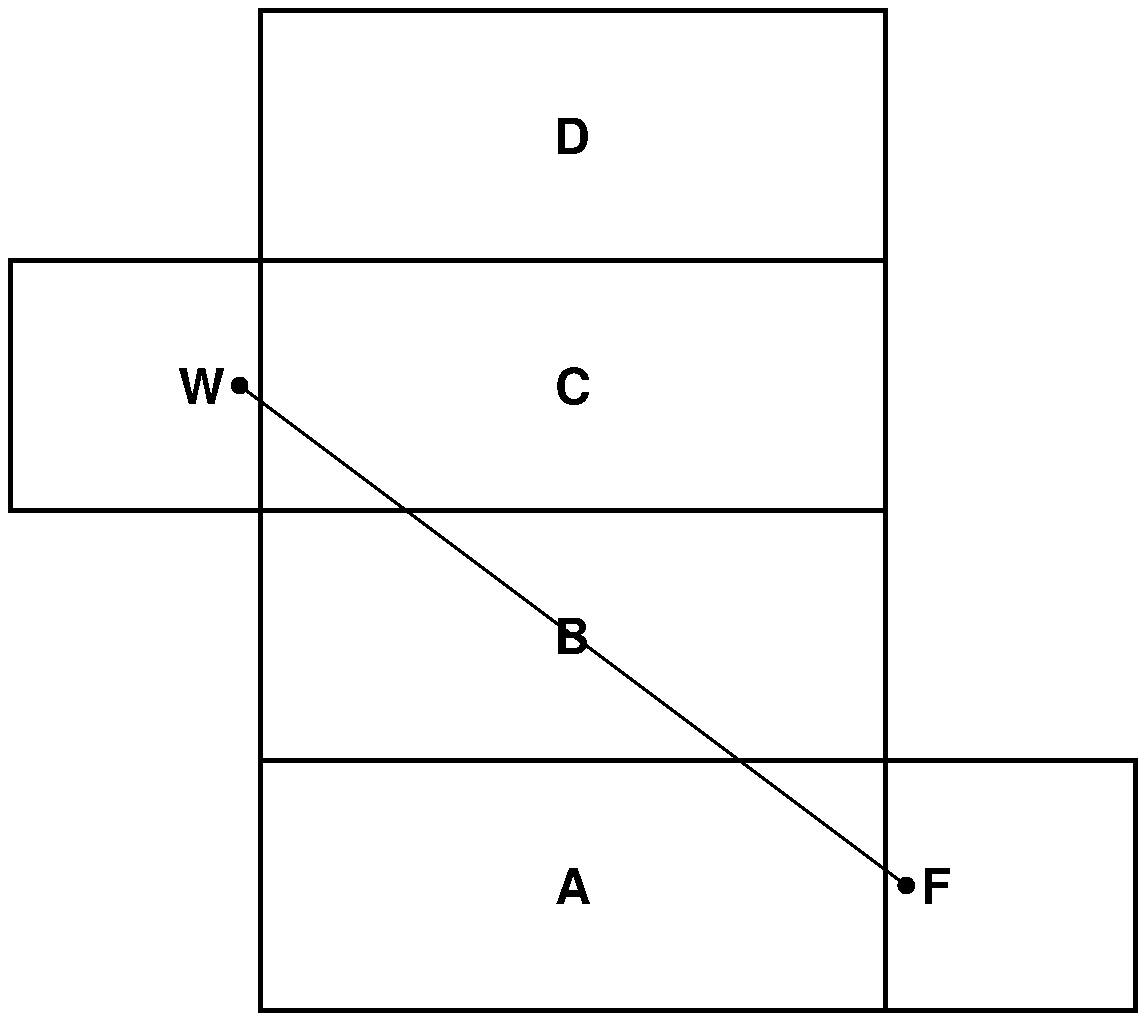
\includegraphics
[height=\ifPaper8cm\else.7\textheight\fi]{./images/illus084}\DPlabel{illus084}}
\end{figure*}

\vhyperlink{illus084}{Here} is the diagram corresponding to a solution of the
above question, where $A$ represents the floor, $B$ and $D$ the
longer side-walls, $C$ the ceiling, and $W$ and $F$ the positions on
the two smaller side-walls occupied initially by the wasp and
fly. In the diagram the square of the distance between $W$
and $F$ is $(32)^2 + (24)^2$; hence the distance is $40$ feet\index
{Geodesic@\textsc{Geodesic Problems}|)}.

\subsection[Problems with Counters placed in a row][Problems with Counters.]%
{Problems with Counters placed in a row}
Numerous dynamical%
\index{Counters, Games with|(}%
\index{GamesWith@\nobreak--- with Counters|(}%
\index{Pawns@\textsc{Pawns, Games with}|(}%
\index{Row, Counters in a|(}
problems and puzzles may be illustrated with a box of
counters, especially if there are counters of two colours. Of
course coins or pawns or cards will serve equally well. I proceed
to enumerate a few of these played with counters placed
in a row.

\subsection*{First Problem with Counters} The following problem must
be familiar to many of my readers. Ten counters (or coins) are
placed in a row. Any counter may be moved over two of
\PG----File: 085.png--------------------------------------------------
those adjacent to it on the counter next beyond them. It is
required to move the counters according to the above rule so
that they shall be arranged in five equidistant couples.

If we denote the counters in their initial positions by the
numbers $1$, $2$, $3$, $4$, $5$, $6$, $7$, $8$, $9$, $10$, we proceed as
 follows. Put
$7$ on $10$, then $5$ on $2$, then $3$ on $8$, then $1$ on $4$, and lastly
 $9$ on
$6$. Thus they are arranged in pairs on the places originally
occupied by the counters $2$, $4$, $6$, $8$, $10$.

Similarly by putting $4$ on $1$, then $6$ on $9$, then $8$ on $3$, then
$10$ on $7$, and lastly $2$ on $5$, they are arranged in pairs on the
places originally occupied by the counters $1$, $3$, $5$, $7$, $9$.

If two superposed counters are reckoned as only one,
solutions analogous to those given above will be obtained by
putting $7$ on $10$, then $5$ on $2$, then $3$ on $8$, then $1$ on $6$, and
lastly $9$ on $4$; or by putting $4$ on $1$, then $6$ on $9$, then $8$ on $3$,
then $10$ on $5$, and lastly $2$ on $7$\footnote
{Note by J.~Fitzpatrick\index{Fitzpatrick, J.} to a French translation of the
third edition of this work, Paris, 1898.}.

There is a somewhat similar game played with eight counters,
but in this case the four couples finally formed are not equidistant.
Here the transformation will be effected if we move
$5$ on $2$, then $3$ on $7$, then $4$ on $1$, and lastly $6$ on $8$. This form
of the game is applicable equally to $(8 + 2n)$ counters, for if we
move $4$ on $1$ we have left on one side of this couple a row of
$(8 + 2n - 2)$ counters. This again can be reduced to one of
$(8 + 2n - 4)$ counters, and in this way finally we have left $8$
counters which can be moved in the way explained above.

A more complete generalization would be the case of $n$
counters, where each counter might be moved over the $m$
counters adjacent to it on to the one beyond them.

\subsection*{Second Problem with Counters} Another problem of a
somewhat similar kind is due to Tait\index{Tait}\footnote
{\textit{Philosophical Magazine}, London, January, 1884, series~5,
vol.~\textsc{xvii}, p.~39.}. Place four florins
(or white counters) and four halfpence (or black counters)
alternately in a line in contact with one another. It is required
\PG----File: 086.png--------------------------------------------------
in four moves, each of a pair of two contiguous pieces,
without altering the relative position of the pair, to form
a continuous line of four halfpence followed by four florins.

His solution is as follows. Let a florin be denoted by $a$
and a halfpenny by $b$, and let $\times \times$ denote two contiguous
blank spaces. Then the successive positions of the pieces may
be represented thus:
\[
\def\arraycolsep{4pt}
\begin{array}{>{$}l<{\dotfillatleast3$}cccccccccc@{.}}
Initially&\times&\times&a&b&a&b&a&b&a&b\\
After the first move&b&a&a&b&a&b&a&\times&\times&b\\
After the second move&b&a&a&b&\times&\times&a&a&b&b\\
After the third move&b&\times&\times&b&a&a&a&a&b&b\\
After the fourth move&b&b&b&b&a&a&a&a&\times&\times\\
\end{array}
\]

The operation is conducted according to the following rule.
Suppose the pieces to be arranged originally in circular order,
with two contiguous blank spaces, then we always move to
the blank space for the time being that pair of coins which
occupies the places next but one and next but two to the
blank space on one assigned side of it.

A similar problem with $2n$ counters---$n$ of them being
white and $n$ black---will at once suggest itself, and, if $n$ is
greater than $4$, it can be solved in $n$ moves. I have however
failed to find a simple rule which covers all cases alike, but
solutions, due to M.~Delannoy\index{Delannoy}, have been given\footnote
{\textit{La Nature}, June, 1887, p.~10.} for the four
cases where $n$ is of the form $4m$, $4m + 2$, $4m + 1$, or $4m + 3$; in
the first two cases the first $\frac{1}{2}n$ moves are of pairs of dissimilar
counters and the last $\frac{1}{2}n$ moves are of pairs of similar counters;
in the last two cases, the first move is similar to that given %
% [**Note: original wording 'on the last page' silently altered because
% (a) the reference isn't % accurate (the reference is to the array above) and
% (b) it's easier than trying to decide if there's an intervening page break
% in the LaTeX version
above, namely, of the penultimate and antepenultimate
counters to the beginning of the row, the next $\frac{1}{2} (n - 1)$ moves
are of pairs of dissimilar counters, and the final $\frac{1}{2} (n - 1)$
moves are of similar counters.

The problem is also capable of solution if we substitute
the restriction that at each move the pair of counters taken up
\PG----File: 087.png--------------------------------------------------
must be moved to one of the two ends of the row instead of
the condition that the final arrangement is to be continuous.

Tait\index{Tait} suggested a variation of the problem by making it a
condition that the two coins to be moved shall also be made to
interchange places; in this form it would seem that $5$ moves are
required; or, in the general case, $n + 1$ moves are required.

\subsection[Problems on a Chess-board with Counters or Pawns]%
[Problems with Counters or Pawns]%
{Problems on a Chess-board with Counters or Pawns} The
following three problems require the use of a chess-board as well%
\index{Chess-board, Games@\textsc{Chess-board, Games on}|(}%
\index{Chess-board, problems@\nobreak--- problems|(}
as of counters or pieces of two colours. It is more convenient
to move a pawn than a counter, and if therefore I describe them
as played with pawns it is only as a matter of convenience and
not that they have any connection with chess. The first is
characterized by the fact that in every position not more than
two moves are possible; in the second and third problems not
more than four moves are possible in any position. With these
limitations, analysis is possible. I shall not discuss the similar
problems in which more moves are possible.

\subsection*{First Problem with Pawns\protect\footnote
{Lucas\index{Lucas, E.}, vol.~\textsc{ii}, part~5, pp.~141-143.}}
On a row of seven squares
on a chess-board $3$ white pawns (or counters), denoted in the
diagram by ``$a$''s, are placed on the $3$ squares at one end, and
$3$ black pawns (or counters), denoted by ``$b$''s, are placed on
the $3$ squares at the other end---the middle square being left
vacant. Each piece can move only in one direction; the ``$a$''
pieces can move from left to right, and the ``$b$'' pieces from
right to left. If the square next to a piece is unoccupied, it
\begin{figure*}[!h]
\centering
\begin{picture}(7,1)
\Cell(0,0;a)
\Cell(1,0;a)
\Cell(2,0;a)
\Cell(3,0; )
\Cell(4,0;b)
\Cell(5,0;b)
\Cell(6,0;b)
\end{picture}
\end{figure*}
can move on to that; or if the square next to it is occupied by
a piece of the opposite colour and the square beyond that is
unoccupied, then it can, like a queen in draughts, leap over
that piece on to the unoccupied square beyond it. The object
is to get all the white pawns in the places occupied initially
by the black pawns and vice versa.

The solution requires $15$ moves.  It may be effected by
moving first a white pawn, then successively two black pawns
\PG----File: 088.png--------------------------------------------------
then three white pawns, then three black pawns, then three
white pawns, then two black pawns, and then one white pawn.
We can express this solution by saying that if we number the
cells (a term used to describe each of the small squares on a
chess-board) consecutively, then initially the vacant space
occupies the cell $4$ and in the successive moves it will occupy
the cells $3$, $5$, $6$, $4$, $2$, $1$, $3$, $5$, $7$, $6$, $4$, $2$, $3$,
$5$, $4$. Of these moves, six are simple and nine are leaps.

Similarly if we have $n$ white pawns at one end of a row
of $2n + 1$ cells, and $n$ black pawns at the other end, they can
be interchanged in $n (n + 2)$ moves, by moving in succession
$1$ pawn, $2$ pawns, $3$ pawns,~\ldots, $n - 1$ pawns, $n$ pawns, $n$ pawns,
$n$ pawns, $n - 1$ pawns,~\ldots, $2$ pawns, and $1$ pawn---all the pawns
in each group being of the same colour and different from
that of the pawns in the group preceding it. Of these moves
$2n$ are simple and $n^2$ are leaps\index{Row, Counters in a|)}.

\subsection*{Second Problem with Pawns\protect\footnote
{Lucas\index{Lucas, E.}, vol.~\textsc{ii}, part~5, p.~144.}}
A similar game may be
played on a rectangular or square board. The case of a square
board containing $49$ cells, or small squares, will illustrate this
sufficiently: in this case the initial position is shown in the
annexed diagram where the ``$a$''s denote the pawns or pieces
\begin{figure*}[!hbt]
\centering
\begin{MagicSquare}{7}
 a & a & a & a & b & b & b \\
 a & a & a & a & b & b & b \\
 a & a & a & a & b & b & b \\
 a & a & a & {} & b & b & b \\
 a & a & a & b & b & b & b \\
 a & a & a & b & b & b & b \\
 a & a & a & b & b & b & b
\end{MagicSquare}
\end{figure*}
of one colour, and the ``$b$''s those of the other colour. The ``$a$''
pieces can move horizontally from left to right or vertically
down, and the ``$b$'' pieces can move horizontally from right to
left or vertically up, according to the same rules as before.

\PG----File: 089.png-----------------------------------------------------
The solution reduces to the preceding case. The pieces
in the middle column can be interchanged in $15$ moves. In
the course of these moves every one of the seven cells in that
column is at some time or other vacant, and whenever that
is the case the pieces in the row containing the vacant cell
can be interchanged. To interchange the pieces in each of
the seven rows will require 15 moves. Hence to interchange all
the pieces will require $15 + (7 \times 15)$ moves, that is, $120$ moves.

If we place $2n(n + 1)$ white pawns and $2n(n + 1)$ black
pawns in a similar way on a square board of $(2n + 1)^2$ cells,
we can transpose them in $2n (n + 1)(n + 2)$ moves: of these
$4n(n + 1)$ are simple and $2n^2 (n + 1)$ are leaps.

\subsection*{Third Problem with Pawns} The following analogous,
though somewhat more complicated, game was I believe
originally published in the first edition of this work: but I find
\begin{figure*}[!hbt]
\centering
\begin{picture}(5,5)
\Cell(0,4;a)\Cell(1,4;b)\Cell(2,4;c)\Cell(3,4; )\Cell(4,4; )
\Cell(0,3;d)\Cell(1,3;e)\Cell(2,3;f)\Cell(3,3; )\Cell(4,3; )
\Cell(0,2;g)\Cell(1,2;h)\Cell(2,2;*)\Cell(3,2;H)\Cell(4,2;G)
\Cell(0,1; )\Cell(1,1; )\Cell(2,1;F)\Cell(3,1;E)\Cell(4,1;D)
\Cell(0,0; )\Cell(1,0; )\Cell(2,0;C)\Cell(3,0;B)\Cell(4,0;A)
\put(0,2){\line(0,1){3}}
\put(0,2){\line(1,0){2}}
\put(0,5){\line(1,0){3}}
\put(2,0){\line(0,1){2}}
\put(2,0){\line(1,0){3}}
\put(5,0){\line(0,1){3}}
\put(3,3){\line(1,0){2}}
\put(3,3){\line(0,1){2}}
\end{picture}
\end{figure*}
that it has been since widely distributed in connexion with an
advertisement and probably now is well-known. On a square
board of 25 cells, place eight white pawns or counters on the
cells denoted by small letters in the annexed diagram, and
eight black pawns or counters on the cells denoted by capital
letters: the cell marked with an asterisk ($*$) being left blank.
Each pawn can move according to the laws already explained---the
white pawns being able to move only horizontally from
left to right or vertically downwards, and the black pawns being
able to move only horizontally from right to left or vertically
upwards. The object is to get all the white pawns in the
places initially occupied by the black pawns and vice versa.
No moves outside the dark line are permitted.

\PG----File: 090.png------------------------------------------------------
Since there is only one cell on the board which is unoccupied,
and since no diagonal moves and no backward moves are
permitted, it follows that at each move not more than two
pieces of either colour are capable of moving. There are however
a very large number of solutions. The following empirical
solution in forty-eight moves is one way of effecting the transfer---the
letters indicating the cells \emph{from} which the pieces are
successively moved:
\[\def\arraycolsep{2pt}
\begin{array}{ccccccccccccccccccccccccc}
h&H&*&f&F&E&H&G&*&c&b&h&g&d&f&F&C&*&h&H&B&A&C&*\\
c&a&b&h&H&*&c&f&F&D&G&H&B&C&*&g&h&e&f&F&*&h&H&*\rlap{$\;$.}
\end{array}
\]
It will be noticed that the first twenty-four moves lead to a
symmetrical position, and that the next twenty-three moves
can be at once obtained by writing the first twenty-three
moves in reverse order and interchanging small and capital
letters\index{Counters, Games with|)}%
\index{GamesWith@\nobreak--- with Counters|)}%
\index{Pawns@\textsc{Pawns, Games with}|)}.

Probably, were it worth the trouble, the mathematical
theory of games such as that just described might be worked
out by the use of Vandermonde's\index{Vandermonde} notation, described later
in \hyperlink{section*.140}{chapter~\textsc{vi}}, or by the analogous method
employed in the theory of the game of solitaire\footnote
{On the theory of the solitaire, see Reiss\index{Reiss}, `\textit{Beiträge
zur Theorie des Solitär-Spiels},' \textit{Crelle's Journal}, Berlin, 1858,
vol.~\textsc{liv}, pp.~344--379; and
Lucas\index{Lucas, E.}, vol.~\textsc{i}, part~\textsc{v}, pp.~89--141.
}. I believe that this has not been
done, and I do not think it would repay the labour involved.

\markright{Problems with Chess-pieces}
\subsection*{Problems on a Chess-board with Chess-pieces} There are
several mathematical recreations with chess-pieces, other than
pawns, somewhat similar to those given above. One of these,
on the determination of the ways in which eight queens can be
placed on a board so that no queen can take any other, is given
later in \hyperlink{section.4.4}{chapter~\textsc{iv}}.
Another, on the path to be followed by a
knight which is moved on a chess-board so that it shall occupy
every cell once and only once, is given in \hyperlink
{section.6.5}{chapter~\textsc{vi}}. Here
I will mention one of the simplest of such problems, which is
interesting from the fact that it is given in Guarini's manuscript
\PG----File: 091.png------------------------------------------------------
written in 1512; it was quoted by Lucas\index{Lucas, E.}, but so far as
I know has not been otherwise published.

\subsection*{Guarini's Problem}%
\addcontentsline{toc}{subsection}{Guarini's Problem}
On a board of nine cells\index{Guarini's Problem}, such as that\index
{Chess-board, knights@\nobreak--- knights' moves on}
drawn below, the two white knights are placed on the two top
\begin{figure*}[!hbt]
\centering
\begin{MagicSquare}{3}
a & C & d\\
D & {} & B\\
b & A & c
\end{MagicSquare}
\end{figure*}
corner cells ($a$,~$d$), and the two black knights on the two
bottom corner cells ($b$,~$c$): the other cells are left vacant. It
is required to move the knights so that the white knights shall
occupy the cells $b$ and $c$, while the black shall occupy the cells
$a$ and $d$.

The solution is tolerably obvious. First, move the pieces
from $a$ to $A$, from $b$ to $B$, from $c$ to $C$, and from $d$ to $D$. Next,
move the pieces from $A$ to $d$, from $B$ to $a$, from $C$ to $b$, and
from $D$ to $c$. The effect of these eight moves is the same as if
the original square had been rotated through one right angle.
Repeat the above process, that is, move the pieces successively
from $a$ to $A$, from $b$ to $B$, from $c$ to $C$, from $d$ to $D$; from $A$
to $d$, from $B$ to $a$, from $C$ to $b$, and from $D$ to $c$. The required
result is then attained%
\index{Chess-board, Games@\textsc{Chess-board, Games on}|)}%
\index{Chess-board, problems@\nobreak--- problems|)}%
\index{Dynamical@\textsc{Dynamical Games}|)}%
\index{Games@\textsc{Games}, Dynamical|)}.

\section[Geometrical Puzzles (rods, strings, \protect\&c.)]%
[Geometrical Puzzles]{Geometrical Puzzles with Rods, etc} Another species
of geometrical puzzles, to which here I will do no more than
allude, are made of steel rods, or of wire, or of wire and string.
Numbers of these are often sold in the streets of London
for a penny each, and some of them afford ingenious problems
in the geometry of position. Most of them could hardly
be discussed without the aid of diagrams, but they are
inexpensive to construct, and in fact innumerable puzzles
on geometry of position can be made with a couple of
stout sticks and a ball of string, or even with only a box
of matches: several examples are given in the appendix to
the fourth volume of the 1723 edition of Ozanam's\index
{Ozanam@Ozanam's \textit  {Récréations}} work.
\PG----File: 092.png-----------------------------------------------------
I will mention, as an easy example, analogous to one group
of the string puzzles, that any one can take off his waistcoat
(which may be unbuttoned) without taking off his coat\index
{Coat and Waistcoat Trick}, and
without pulling the waistcoat over the head like a jersey.

This last feat may serve to show the difficulty of mentally
realizing the effect of geometrical alterations in a figure unless
they are of the simplest character.

\section{Paradromic Rings} The fact just stated is illustrated
by the familiar experiment of making \emph{paradromic rings}\index
{Paradromic@\textsc{Paradromic Rings}|(} by
cutting a paper ring prepared in the following manner.

Take a strip of paper or piece of tape, say, for convenience,
an inch or two wide and at least nine or ten inches long,
rule a line in the middle down the length $AB$ of the strip,
gum one end over the other end $B$, and we get a ring like
a section of a cylinder. If this ring is cut by a pair of scissors
along the ruled line we obtain two rings exactly like the first,
except that they are only half the width. Next suppose that
the end $A$ is twisted through two right angles before it is
gummed to $B$ (the result of which is that the back of the
strip at $A$ is gummed over the front of the strip at $B$), then a
cut along the line will produce only one ring. Next suppose
that the end $A$ is twisted once completely round (\IE\ through
four right angles) before it is gummed to $B$, then a similar cut
produces two interlaced rings. If any of my readers think
that these results could be predicted off-hand, it may be
interesting to them to see if they can predict correctly the
effect of again cutting the rings formed in the second and
third experiments down their middle lines in a manner similar
to that above described.

The theory is due to J.B.~Listing\index
{Listing@Listing's \textit{Topologie}}\footnote
{\textit{Vorstudien zur Topologie, Die Studien}, Göttingen, 1847,
part~\textsc{x}.} who discussed the case
when the end $A$ receives $m$ half-twists, that is, is twisted
through $m\pi$, before it is gummed to $B$.

If $m$ is even we obtain a surface which has two sides and
\PG----File: 093.png----------------------------------------------------
two edges, which are termed paradromic. If the ring is cut
along a line midway between the edges, we obtain two rings,
each of which has $m$ half-twists, and which are linked together
$\frac{1}{2}m$ times.

If $m$ is odd we obtain a surface having only one side and
one edge. If this ring is cut along its mid-line, we obtain
only one ring, but it has $2m$ half-twists, and if $m$ is greater
than unity it is knotted\index{Paradromic@\textsc{Paradromic Rings}|)}%
\index{PuzzlesGeom@\nobreak--- Geometrical|)}.

\PG----File: 094.png----------------------------------------------------



%CHAPTER III.

\chapter[Some Mechanical Questions.][Mechanical Recreations.]%
{Some Mechanical Questions.}

\textsc{I proceed} now to enumerate a few questions connected\chapindex
{Mechanical Recreations@\textsc{Mechanical Recreations}}
with mechanics which lead to results that seem to me interesting
from a historical point of view or paradoxical. Problems
in mechanics generally involve more difficulties than
problems in arithmetic, algebra, or geometry, and the explanations
of some phenomena---such as those connected with the
flight of birds---are still incomplete, while the explanations of
many others of an interesting character are too difficult to
find a place in a non-technical work. Here, however, I shall
confine myself to questions which, like those treated in the
two preceding chapters, are of an elementary, not to say
trivial, character; and the conclusions are well-known to
mathematicians.

I assume that the reader is acquainted with the fundamental
ideas of kinematics and dynamics, and is familiar with
the three Newtonian laws\index{MotionLaw@Motion, Laws of}\index
{Newtonian Laws of Motion|(}; namely, first that a body will
continue in its state of rest or of uniform motion in a straight
line unless compelled to change that state by some external
force: second, that the change of momentum per unit of time
is proportional to the external force and takes place in the
direction of it: and third, that the action of one body on
another is equal in magnitude but opposite in direction to
the reaction of the second body on the first. The first and
second laws state the principles required for solving any
question on the motion of a particle under the action of given
\PG----File: 095.png------------------------------------------------------
forces. The third law supplies the additional principle required
for the solution of problems in which two or more particles
influence one another.

\section[Paradoxes on Motion][Zeno's Paradoxes.]{Motion}
The difficulties connected with the idea of \emph{motion}
have been for a long time a favourite subject for paradoxes%
\index{MotionParadox@\nobreak--- Paradoxes on|(}%
\index{PuzzlesMech@\nobreak--- Mechanical|(},
some of which bring us into the realm of the philosophy of
mathematics.

\subsection*{Zeno's Paradoxes on Motion} One of the earliest of these\index
{Zeno on Motion|(}\index{FallaciesMech@\nobreak--- \textsc{Mechanical}|(}
is the remark of Zeno to the effect that since an arrow cannot
move where it is not, and since also it cannot move where it
is (\IE\ in the space it exactly fills), it follows that it cannot
move at all. The answer that the very idea of the motion of
the arrow implies the passage from where it is to where it is
not was rejected by Zeno, who seems to have thought that the
appearance of motion of a body was a phenomenon caused by
the successive appearances of the body at rest but in different
positions.

Zeno also asserted that the idea of motion was itself
inconceivable, for what moves must reach the middle of its
course before it reaches the end. Hence the assumption of
motion presupposes another motion, and that in turn another,
and so ad infinitum. His objection was in fact analogous to
the biological difficulty expressed by Swift\index{Swift}:---
\begin{verse}\small
\leavevmode\llap{``}%
So naturalists observe, a flea hath smaller fleas that on him prey.\\
And these have smaller fleas to bite 'em. And so proceed ad infinitum.''
\end{verse}

\bigskip
\noindent Or as De~Morgan\index{DeMorgan@De Morgan, A.} preferred to put it
\begin{verse}\small
\leavevmode\llap{``}%
Great fleas have little fleas upon their backs to bite 'em,\\
And little fleas have lesser fleas, and so ad infinitum.\\
And the great fleas themselves, in turn, have greater fleas to go on;\\
While these have greater still, and greater still, and so on.''
\end{verse}

\ThoughtBreakSpace
\subsection*{Achilles and the Tortoise} Zeno's paradox about Achilles\index
{Achilles and the Tortoise}
and the tortoise is known even more widely. The assertion
was that if Achilles ran ten times as fast as a tortoise, yet
if the tortoise had (say) $1000$ yards start it could never be
\PG----File: 096.png-------------------------------------------------------
overtaken. To establish this, Zeno argued that when Achilles
had gone the $1000$ yards, the tortoise would still be $100$ yards
in front of him; by the time he had covered these $100$ yards,
it would still be $10$ yards in front of him; and so on for ever.
Thus Achilles would get nearer and nearer to the tortoise
but would never overtake it. Zeno regarded this as confirming
his view that the popular idea of motion is self-contradictory.

\subsection*{Zeno's Paradox on Time} The fallacy of Achilles and
the Tortoise is usually explained by saying that though the
time required to overtake the tortoise can be divided into an
infinite number of intervals, as stated in the argument, yet
these intervals get smaller and smaller in geometrical progression,
and the sum of them all is a finite time: after the lapse of
that time Achilles would be in front of the tortoise. Probably
Zeno would have replied that this explanation rests on the
assumption that space and time are infinitely divisible,
propositions which he would not admit. He seems further
to have contended that while, to an accurate thinker, the
notion of the infinite divisibility of time was impossible, it
was equally impossible to think of a minimum measure of
time. For suppose, he argued, that $\tau$ is the smallest conceivable
interval, and suppose that three horizontal lines composed
of three consecutive spans $abc$, $a'b'c'$, $a''b''c''$ are placed so
that $aa'a''$, $bb'b''$, $cc'c''$ are vertically over one another. Imagine
the second line moved as a whole one span to the right in the
time $\tau$, and simultaneously the third line moved as a whole
one span to the left. Then $b$, $a'$, $c''$ will be vertically over
one another. And in this duration $\tau$ (which by hypothesis is
indivisible) $c'$ must have passed vertically over $a''$. Hence the
duration is divisible, contrary to the hypothesis\index{Zeno on Motion|)}.

\markright{The Paradox of Tristram Shandy.}
\subsection*{The Paradox of Tristram Shandy} Mr~Russell\index
{Russell, B.A.W.} has enunciated\footnote
{B.A.W.~Russell, \textit{Principles of Mathematics}, Cambridge, 1903,
vol.~\textsc{i}, p.~358.
} a paradox somewhat similar to that of Achilles and
the Tortoise, save that the intervals of time considered get
\PG----File: 097.png-----------------------------------------------------
longer and longer during the course of events. Tristram
Shandy, as we know, took two years writing the history of
the first two days of his life, and lamented that, at this rate,
material would accumulate faster than he could deal with it,
so that he could never come to an end, however long he lived.
But had he lived long enough, and not wearied of his task,
then, even if his life had continued as eventfully as it began,
no part of his biography would have remained unwritten.
For if he wrote the events of the first day in the first year, he
would write the events of the $n$th day in the $n$th year, hence
in time the events of any assigned day would be written, and
therefore no part of his biography would remain unwritten.
This argument might be put in the form of a demonstration
that the part of a magnitude may be equal to the whole of it.

Questions, such as those given above, which are concerned
with the continuity and extent of space and time involve
difficulties of a high order.

\markright{Angular Motion.}
\subsection*{Angular Motion} A non-mathematician finds additional\index
{Angular Motion}
difficulties in the idea of angular motion. For instance, here
is a well-known proposition on motion in an equiangular spiral
(of which the result is true on the ordinary conventions of
mathematics) which shows that a body, moving with uniform
velocity and as slowly as we please, may in a finite time whirl
round a fixed point an infinite number of times.

The equiangular spiral is the trace of a point $P$, which
moves along a line $OP$, the line $OP$ turning round a fixed
point $O$ with uniform angular velocity while the distance of
$P$ from $O$ decreases with the time in geometrical progression.
If the radius vector rotates through four right angles we have
one convolution of the curve. All convolutions are similar,
and the length of each convolution is a constant fraction, say
$1/n$th, that of the convolution immediately outside it. Inside
any given convolution, there are an infinite number of convolutions
which get smaller and smaller as we get nearer the
pole. Now suppose a point $Q$ to move uniformly along the
spiral from any point towards the pole. If it covers the first
\PG----File: 098.png-----------------------------------------------------
convolution in $a$ seconds, it will cover the next in $a/n$ seconds,
the next in $a/n^2$ seconds, and so on, and will finally reach the
pole in $(a + a/n + a/n^2 + a/n^3 + \dotsb)$ seconds, that is, in
$an/(n-1)$ seconds. The velocity is uniform, and yet in a finite
time, $Q$ will have traversed an infinite number of convolutions
and therefore have circled round the pole an infinite number
of times\footnote
{The proposition is put in this form in J.~Richard's\index
{Richard, J.} \textit{Philosophie des
math\-é\-mat\-iques}, Paris, 1903, pp.~119--120.}\index
{MotionParadox@\nobreak--- Paradoxes on|)}.

\markright{Simple Relative Motion.}
\subsection*{Simple Relative Motion} Even if the philosophical difficulties
suggested by Zeno are settled or evaded, the mere idea
of relative motion\index
{Relative Motion} has been often found to present difficulties,
and Zeno himself failed to explain a simple phenomenon
involving the principle. As one of the easiest examples of
this kind, I may quote the common question of how many
trains going from $B$ to $A$ a passenger from $A$ to $B$ would
meet and pass on his way, assuming that the journey either
way takes $4\frac{1}{2}$ hours and that the trains start from each end
every hour. The answer is $9$. Or again this: Take two
pennies, face upwards on a table and edges in contact.
Suppose that one is fixed and that the other rolls on it without
slipping, making one complete revolution round it and
returning to its initial position. How many revolutions round
its own centre has the rolling coin made? The answer is $2$\index
{FallaciesMech@\nobreak--- \textsc{Mechanical}|)}.

\subsection*{Laws of Motion}%
\addcontentsline{toc}{section}{Force, Inertia, Centrifugal Force}%
\markright{Laws of Motion.}%
I proceed next to make a few remarks
on points connected with the laws of motion\index
{MotionLaw@Motion, Laws of|(}.

The first law of motion is often said to define \emph{force}\index
{Force, Definition of}, but
it is in only a qualified sense that this is true. Probably
the meaning of the law is best expressed in Clifford's\index{Clifford} phrase,
that force is ``the description of a certain kind of motion''---in
other words it is not an entity but merely a convenient
way of stating, without circumlocution, that a certain kind of
motion is observed.

It is not difficult to show that any other interpretation
lands us in difficulties. Thus some authors use the law to
justify a definition that force is that which moves a body or
\PG----File: 099.png-------------------------------------------------------
changes its motion; yet the same writers speak of a steam-engine
moving a train. It would seem then that, according
to them, a steam-engine is a force. That such statements are
current may be fairly reckoned among mechanical paradoxes.

The idea of force is difficult to grasp. How many people,
for instance, could predict correctly what would happen in a
question as simple as the following? A rope (whose weight
may be neglected) hangs over a smooth pulley; it has one end
fastened to a weight of $10$ stone, and the other end to a sailor
of weight $10$ stone, the sailor and the weight hanging in the
air. The sailor begins to climb up the rope; will the weight
move at all; and, if so, will it rise or fall?

It will be noted that in the first law of motion it is asserted
that, unless acted on by an external force, a body in motion
continues to move (i)~with uniform velocity, and (ii)~in a
straight line.

The tendency of a body to continue in its state of rest
or of uniform motion is called its \emph{inertia}\index{Inertia}.
This tendency
may be used to explain various common phenomena and
experiments. Thus, if a number of dominoes or draughts are
arranged in a vertical pile, a sharp horizontal blow on one of
those near the bottom will send it out of the pile, and those
above will merely drop down to take its place---in fact they
have not time to change their relative positions before there
is sufficient space for them to drop vertically as if they were a
solid body.

This also is the principle on which depends the successful
playing of ``Aunt Sally,'' and the performance of numerous
tricks, described in collections of mathematical puzzles\footnote
{See \textit{Les récréations scientifiques} by G.~Tissandier\index
{Tissandier}, where several
ingenious illustrations of inertia are given.}.

The statement about inertia\index{Inertia} in the first law may be taken
to imply that a body set in rotation about a principal axis
passing through its centre of mass will continue to move with
a uniform angular velocity and to keep its axis of rotation fixed
in direction. The former of these statements is the assumption
\PG----File: 100.png-----------------------------------------------------
on which our measurement of time is based as mentioned below
in \hyperlink{chapter.13}{chapter~\textsc{xiii}}.
The latter assists us to explain the motion of
a projectile in a resisting fluid. It affords the explanation of
why the barrel of a rifle is grooved; and why, similarly, anyone
who has to throw a flat body of irregular shape (such as a card)
in a given direction usually gives it a rapid rotatory motion
about a principal axis. Elegant illustrations of the fact just
mentioned are afforded by a good many of the tricks of acrobats,
though the full explanation of most of them also introduces
other considerations. Thus when some few years ago the
Japanese village at Knightsbridge was one of the shows of
London, there were some acrobats there who tossed on to the
top surface of an umbrella a penny so that it alighted on its
edge, and then, by turning round the stick of the umbrella
rapidly, the coin was caused to rotate, but as the umbrella
moved away underneath it the coin remained apparently
stationary and standing upright, while by diminishing or increasing
the angular velocity of the umbrella the penny was
caused to run forwards or backwards. This is not a difficult
trick to execute.

The tendency of a body in motion to continue to move
in a straight line is sometimes called its \textit{centrifugal force}\index
{Centrifugal Force|(}.
Thus, if a train is running round a curve, it tends to move in
a straight line, and is constrained only by the pressure of the
rails to move in the required direction. Hence it presses on
the outer rail of the curve. This pressure can be diminished
to some extent both by raising the outer rail, and by putting
a guard rail, parallel and close to the inner rail, against which
the wheels on that side also will press.

An illustration of this fact occurred in a little known incident
of the American civil war\footnote
{\textit{Capturing a Locomotive} by W.~Pittenger\index
{Pittenger}, London, 1882, p.~104.}. In the spring of 1862 a
party of volunteers from the North made their way to the
rear of the Southern armies and seized a train, intending to
destroy, as they passed along it, the railway which was the
main line of communication between various confederate corps
\PG----File: 101.png-------------------------------------------------
and their base of operations. They were however detected
and pursued. To save themselves, they stopped on a sharp
curve and tore up some rails so as to throw the engine which
was following them off the line. Unluckily for themselves
they were ignorant of dynamics and tore up the inner rails of
the curve, an operation which did not incommode their
pursuers\index{Centrifugal Force|)}.

The second law gives us the means of measuring mass,
force, and therefore \emph{work}\index{Work|(}.
A given agent in a given time can
do only a definite amount of work. This is illustrated by the
fact that although, by means of a rigid lever and a fixed
fulcrum, any force however small may be caused to move any
mass however large, yet what is gained in power is lost in
speed---as the popular phrase runs.

Montucla\index{Montucla}\footnote
{Ozanam\index{Ozanam@Ozanam's \textit{Récréations}}, 1803 edition,
vol.~\textsc{ii}, p.~18; 1840 edition, p.~202.}
inserted a striking illustration of this principle
founded on the well-known story of Archimedes\index{Archimedes} who is said
to have declared to Hiero\index
{Hiero of Syracuse} that, were he but given a fixed
fulcrum, he could move the world. Montucla\index{Montucla} calculated the
mass of the earth and, assuming that a man could work incessantly
at the rate of $116$ foot-lbs.\ per second, which is a very
high estimate, he found that it would take over three billion
centuries, \IE\ $3 \times 10^{14}$ years, before a mass equal to that of the
earth was moved as much as one inch against gravity at the
surface of the earth: to move it one inch along a horizonal % [** this isn't a typo!]
plane would take about $74000$ centuries.

\subsection*{Stability of Equilibrium}%
\addcontentsline{toc}{section}{Work, Stability of Equilibrium, \protect\&c.}
It is known to all those who\index
{Equilibrium, Puzzles on|(}\index{Stability of Equilibrium|(}
have read the elements of mechanics that the centre of gravity
of a body, which is resting in equilibrium under its own weight,
must be vertically above its base: also, speaking generally,
we may say that, if every small displacement has the effect of
raising the centre of gravity, then the equilibrium is stable,
that is, the body when left to itself will return to its original
position; but, if a displacement has the effect of lowering the
centre of gravity, then for that displacement the equilibrium
is unstable; while, if every displacement does not alter the
\PG----File: 102.png-----------------------------------------------------
height above some fixed plane of the centre of gravity, then
the equilibrium is neutral. In other words, if in order to cause
a displacement work has to be done against the forces acting
on the body, then for that displacement the equilibrium is
stable, while if the forces do work the equilibrium is unstable.

A good many of the simpler mechanical toys and tricks
afford illustrations of this principle.

\markright{Magic Bottles.}
\subsection*{Magic Bottles\protect\footnote
{Ozanam\index{Ozanam@Ozanam's \textit{Récréations}},
1803 edition, vol.~\textsc{ii}, p.~15; 1840 edition, p.~201.}}
Among the most common of such toys are
the small bottles\index{Magic Bottles}---trays of which may be seen
any day in the
streets of London---which keep always upright, and cannot
be upset until their owner orders them to lie down. Such a
bottle is made of thin glass or varnished paper fixed to the
plane surface of a solid hemisphere or smaller segment of
a sphere. Now the distance of the centre of gravity of a
homogeneous hemisphere from the centre of the sphere is
three-eighths of the radius, and the mass of the glass or
varnished paper is so small compared with the mass of the
lead base that the centre of gravity of the whole bottle is
still within the hemisphere. Let us denote the centre of the
hemisphere by $C$, and the centre of gravity of the bottle by $G$.

If such a bottle is placed with the hemisphere resting on a
horizontal plane and $GC$ vertical, any small displacement on the
plane will tend to raise $G$, and thus the equilibrium is stable.
This may be seen also from the fact that when slightly displaced
there is brought into play a couple, of which one force
is the reaction of the table passing through $C$ and acting
vertically upward, and the other the weight of the bottle
acting vertically downward at $G$. If $G$ is below $C$, this couple
tends to restore the bottle to its original position.

If there is dropped into the bottle a shot or nail so heavy
as to raise the centre of gravity of the whole above $C$, then
the equilibrium is unstable, and, if any small displacement is
given, the bottle falls over on to its side.

Montucla\index{Montucla} says that in his time it was not uncommon to
see boxes of tin soldiers mounted on lead hemispheres, and
\PG----File: 103.png-----------------------------------------------------
when the lid of the box was taken off the whole regiment
sprang to attention.

In a similar way we may explain how to balance a pencil
in a vertical position, with its point resting on the top of one's
finger, an experiment which is described in nearly every book
of puzzles\footnote
{\EG\ Oughtred\index{Oughtreds@Oughtred's \textit{Recreations}},
\textit{Mathematical Recreations}, p.~24; Ozanam\index
{Ozanam@Ozanam's \textit{Récréations}}, 1803
edition, vol.~\textsc{ii}, p.~14; 1840 edition, p.~200.}.
This is effected by taking a penknife, of which
one blade is opened through an angle of (say) $120^{\circ}$, and sticking
the blade in the pencil so that the handle of the penknife is
below the finger. The centre of gravity is thus brought below
the point of support, and a small displacement given to the
pencil will raise the centre of gravity of the whole: thus the
equilibrium is stable.

Other similar tricks are the suspension of a bucket over
the edge of a table by a couple of sticks, and the balancing of
a coin on the edge of a wine-glass by the aid of a couple of
forks\footnote
{Oughtred\index{Oughtreds@Oughtred's \textit{Recreations}}, p.~30;
Ozanam\index{Ozanam@Ozanam's \textit{Récréations}}, 1803 edition,
vol.~\textsc{ii}, p.~12; 1840 edition,
p.~199.}---the
sticks or forks being so placed that the centre of
gravity of the whole is vertically below the point of support
and its depth below it a maximum.

The toy representing a horseman, whose motion continually
brings him over the edge of a table into a position which seems
to ensure immediate destruction, is constructed in somewhat
the same way. A wire has one end fixed to the feet of the
rider; the wire is curved downwards and backwards, and at
the other end is fixed a weight. When the horse is placed so
that his hind legs are near the edge of the table and his forefeet
over the edge, the weight is under his hind feet. Thus
the whole toy forms a pendulum with a curved instead of a
straight rod. Hence the farther it swings over the table, the
higher is the centre of gravity raised, and thus the toy tends
to return to its original position of equilibrium.

An elegant modification of the prancing horse was brought
out at Paris in 1890 in the shape of a toy made of tin and in
\PG----File: 104.png-----------------------------------------------------
the figure of a man\footnote
{\textit{La Nature}, Paris, March, 1891.}. The legs are pivoted
so as to be movable
about the thighs, but with a wire check to prevent too long
a step, and the hands are fastened to the top of a $\bigcap$-shaped
wire weighted at its ends. If the figure is placed on a narrow
sloping plank or strip of wood passing between the legs of the
$\bigcap$, then owing to the $\bigcap$-shaped wire any lateral displacement
of the figure will raise its centre of gravity, and thus for any
such displacement the equilibrium is stable. Hence, if a slight
lateral disturbance is given, the figure will oscillate and will
rest alternately on each foot: when it is supported by one foot
the other foot under its own weight moves forwards, and thus
the figure will walk down the plank though with a slight
reeling motion. Shortly after the publication of the third
edition of this book an improved form of this toy, in the
shape of a walking elephant made in heavy metal, was issued
in England, and probably in that form it is now familiar to
all who are interested in noticing street toys\index
{Equilibrium, Puzzles on|)}\index{Stability of Equilibrium|)}.

\markright{Columbus's Egg.}
\subsection*{Columbus's Egg} The toy known as Columbus's egg\index
{Columbus's Egg Puzzle} depends
on the same principle as the magic bottle, though it leads to
the converse result. The shell of the egg is made of tin and
cannot be opened. Inside it and fastened to its base is a
hollow truncated tin cone, and there is also a loose marble
inside the shell. If the egg is held properly, the marble runs
inside the cone and the egg will stand on its base, but so long
as the marble is outside the cone, the egg cannot be made to
stand on its base.

\markright{Cones running up hill.}
\subsection*{Cones running up hill\protect\footnote
{Ozanam\index{Ozanam@Ozanam's \textit{Récréations}}, 1803 edition,
vol.~\textsc{ii}, p.~49; 1840 edition, p.~216.}} The
experiment to make a double
cone run up hill\index{Cones moving uphill} depends on the same principle
as the toys
above described; namely, on the tendency of a body to take a
position so that its centre of gravity is as low as possible. In
this case it produces the optical effect of a body moving by
itself up a hill.

Usually the experiment is performed as follows. Arrange
two sticks in the shape of a $\bigvee$, with the apex on a table and
\PG----File: 105.png-----------------------------------------------------
the two upper ends resting on the top edge of a book placed
on the table. Take two equal cones fixed base to base, and place
them with the curved surfaces resting on the sticks near the
apex of the $\bigvee$, the common axis of the cones being horizontal
and parallel to the edge of the book. Then, if properly
arranged, the cones will run up the plane formed by the
sticks.

The explanation is obvious. The centre of gravity of the
cones moves in the vertical plane midway between the two
sticks and it occupies a lower position as the points of contact
on the sticks get farther apart. Hence as the cone rolls up
the sticks its centre of gravity descends%
\index{MotionLaw@Motion, Laws of|)}%
\index{Newtonian Laws of Motion|)}%
\index{PuzzlesMech@\nobreak--- Mechanical|)}%
\index{Work|)}.

\section{Perpetual Motion} The idea of making a machine which%
\index{FallaciesMech@\nobreak--- \textsc{Mechanical}|(}%
\index{MotionPerp@\nobreak--- Perpetual|(}%
\index{Perpetual@\textsc{Perpetual Motion}|(}
once set going would continue to go for ever by itself has been
the ignis fatuus of self-taught mechanicians in much the same
way as the quadrature of the circle has been of self-taught
geometricians.

Now the obvious meaning of the third law of motion is
that a force is only one aspect of a stress, and that whenever a
force is caused another equal and opposite one is brought also
into existence---though it may act upon a different body, and
thus be immaterial for the particular problem considered. The
law however is capable of another
interpretation\footnote{Newton's\index{Newton} \textit{Principia}, last
paragraph of the Scholium to the Laws of Motion.}, namely,
that the rate at which an agent does work (that is, its action)
is equal to the rate at which work is done against it (that is,
its reaction). If it is allowable to include in the reaction the
rate at which kinetic energy is being produced, and if work is
taken to include that done against molecular forces, then it
follows from this interpretation that the work done by an
agent on a system is equivalent to the total increase of energy,
that is, the power of doing work. Hence in an isolated system
the total amount of energy is constant. If this is granted,
then since friction and some molecular dissipation of energy
\PG----File: 106.png-----------------------------------------------------
cannot be wholly prevented, it must be impossible to construct
in an isolated system a machine capable of perpetual motion.

I do not propose to describe in detail the various machines
for producing perpetual motion which have been suggested, but
I may add that a number of them are equivalent essentially to
the one of which a section is represented in the accompanying
figure.

\begin{figure*}[!hbt]
\centerline{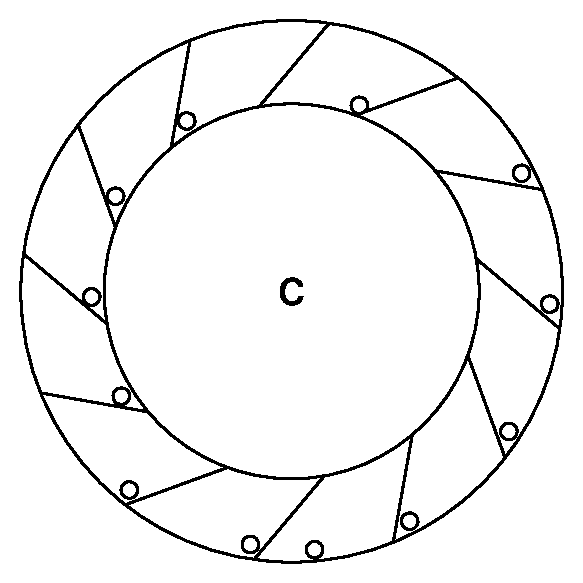
\includegraphics[width=6cm]{./images/illus106}}
\end{figure*}

It consists of two concentric vertical wheels in the same
plane, and mounted on a horizontal axle through their centre, $C$.
The space between the wheels is divided into compartments by
spokes inclined at a constant angle to the radii to the points
whence they are drawn, and each compartment contains a
heavy bullet. Apart from these bullets, the wheels would be
in equilibrium. Each bullet tends to turn the wheels round
their axle, and the moment which measures this tendency is
the product of the weight of the bullet and its distance from
the vertical through $C$.

The idea of the constructors of such machines was that, as
the bullet in any compartment would roll under gravity to the
lowest point of the compartment, the bullets on the right-hand
side of the diagram would be farther from the vertical through
$C$ than those on the left. Hence the sum of the moments of
the weights of the bullets on the right would be greater than
the sum of the moments of those on the left. Thus the wheels
\PG----File: 107.png-----------------------------------------------------
would turn continually in the same direction as the hands of a
watch. The fallacy in the argument is obvious.

Another large group of machines for producing perpetual
motion depended on the use of a magnet to raise a mass which
was then allowed to fall under gravity. Thus, if the bob of a
simple pendulum was made of iron, it was thought that magnets
fixed near the highest points which were reached by the bob in
the swing of the pendulum would draw the bob up to the same
height in each swing and thus give perpetual motion.

Of course it is only in isolated systems that the total amount
of energy is constant, and, if a source of external energy can be
obtained from which energy is continually introduced into the
system, perpetual motion is, in a sense, possible; though even
here materials would ultimately wear out. The solar heat and
the tides are among the most obvious of such sources.

There was at Paris in the latter half of the eighteenth\label
{page:PerpClockStart}
century a clock\index{Clocks} which was an ingenious illustration of such
perpetual motion\footnote
{Ozanam\index{Ozanam@Ozanam's \textit{Récréations}}, 1803 edition,
vol.~\textsc{ii}, p.~105; 1840 edition, p.~238.}. The energy which was
stored up in it to
maintain the motion of the pendulum was provided by the
expansion of a silver rod. This expansion was caused by the
daily rise of temperature, and by means of a train of levers it
wound up the clock. There was a disconnecting apparatus, so
that the contraction due to a fall of temperature produced no
effect, and there was a similar arrangement to prevent overwinding.
I believe that a rise of eight or nine degrees
Fahrenheit was sufficient to wind up the clock for twenty-four
hours.

I have in my possession a watch\index{Watches}, which produces the
same effect by somewhat different means. Inside the case
is a steel weight, and if the watch is carried in a pocket this
weight rises and falls at every step one takes, somewhat after
the manner of a pedometer. The weight is raised by the
action of the person who has it in his pocket in taking a
step, and in falling it winds up the spring of the watch.
On the face is a small dial showing the number of hours for
\PG----File: 108.png-----------------------------------------------------
which the watch is wound up. As soon as the hand of this
dial points to fifty-six hours, the train of levers which winds
up the watch disconnects automatically, so as to prevent overwinding
the spring, and it reconnects again as soon as the
watch has run down eight hours. The watch\index{Watches} is an excellent
time-keeper, and a walk of about a couple of miles is sufficient
to wind it up for twenty-four hours%
\index{MotionPerp@\nobreak--- Perpetual|)}%
\index{Perpetual@\textsc{Perpetual Motion}|)}%
\label{page:PerpClockEnd}.

\section{Models} I may add here the observation, which is well\index
{Models@\textsc{Models}|(}
known to mathematicians, but is a perpetual source of disappointment
to ignorant inventors, that it frequently happens
that an accurate model of a machine will work satisfactorily
while the machine itself will not do so.

One reason for this is as follows. If all the parts of a model
are magnified in the same proportion, say $m$, and if thereby a
line in it is increased in the ratio $m:1$, then the areas and
volumes in it will be increased respectively in the ratios $m^2:1$
and $m^3:1$. For example, if the side of a cube is doubled then
a face of it will be increased in the ratio $4: 1$ and its volume
will be increased in the ratio $8:1$.

Now if all the linear dimensions are increased $m$ times,
then some of the forces that act on a machine (such, for
example, as the weight of part of it) will be increased $m^3$ times,
while others which depend on area (such as the sustaining
power of a beam) will be increased only $m^2$ times. Hence the
forces that act on the machine and are brought into play by
the various parts may be altered in different proportions, and
thus the machine may be incapable of producing results similar
to those which can be produced by the model.

The same argument has been adduced in the case of animal
life to explain why very large specimens of any particular breed
or species are usually weak. For example, if the linear dimensions
of a bird were increased $n$ times, the work necessary to
give the power of flight would have to be increased no less
than $n^7$ times\footnote
{Helmholtz\index{Helmholtz}\index{Von Helmholz}, \textit{Gesammelte
Abhandlungen}, Leipzig, 1881, vol.~\textsc{i}, p.~165.}. Again, if the
linear dimensions of a man
\PG----File: 109.png------------------------------------------------------
of height $5$~ft.\ $10$~in.\ were increased by one-seventh his height
would become $6$~ft.\ $8$~in., but his weight would be increased
in the ratio $512: 343$ (\IE\ about half as much again), while
the cross sections of his legs, which would have to bear this
weight, would be increased only in the ratio $64:49$; thus
in some respects he would be less efficient than before. Of
course the increased dimensions, length of limb, or size of
muscle might be of greater advantage than the relative loss
of strength; hence the problem of what are the most efficient
proportions is not simple, but the above argument will serve
to illustrate the fact that the working of a machine may not
be similar to that of a model of it\index
{FallaciesMech@\nobreak--- \textsc{Mechanical}|)}\index{Models@\textsc{Models}|)}.

\ThoughtBreakSpace
Leaving now these elementary considerations I pass on to
some other mechanical questions.

\ssection{Sailing quicker than the Wind} As a kinematical
paradox I may allude to the possibility of \emph{sailing quicker than
the wind blows}\index{Sailing@\textsc{Sailing}, Theory of|(},
a fact which strikes many people as curious.

The explanation\footnote
{Ozanam\index{Ozanam@Ozanam's \textit{Récréations}}, 1803 edition,
vol.~\textsc{iii}, pp.~359, 367; 1840 edition, pp.~540,
543.} depends on the consideration of the
velocity of the wind relative to the boat. Perhaps, however,
a non-mathematician will find the solution simplified if I consider
first the effect of the wind-pressure on the back of the
sail which drives the boat forward, and second the resistance
to motion caused by the sail being forced through the air.

When the wind is blowing against a plane sail the resultant
pressure of the wind on the sail may be resolved into two
components, one perpendicular to the sail (but which in general
is not a function only of the component velocity in that direction,
though it vanishes when that component vanishes) and
the other parallel to its plane. The latter of these has no
effect on the motion of the ship. The component perpendicular
to the sail tends to move the ship in that direction.
This pressure, normal to the sail, may be resolved again into
two components, one in the direction of the keel of the boat,
\PG----File: 110.png------------------------------------------------------
the other in the direction of the beam of the boat. The
former component drives the boat forward, the latter to leeward.
It is the object of a boat-builder to construct the boat
on lines so that the resistance of the water to motion forward
shall be as small as possible, and the resistance to motion in
a perpendicular direction (\IE\ to leeward) shall be as large as
possible; and I will assume for the moment that the former
of these resistances may be neglected, and that the latter is
so large as to render motion in that direction impossible.

Now, as the boat moves forward, the pressure of the air
on  the front of the sail will tend to stop the motion. As
long as its component normal to the sail is less than the
pressure of the wind behind the sail and normal to it, the
resultant of the two will be a force behind the sail and normal
\begin{figure*}[!hbt]
\centerline{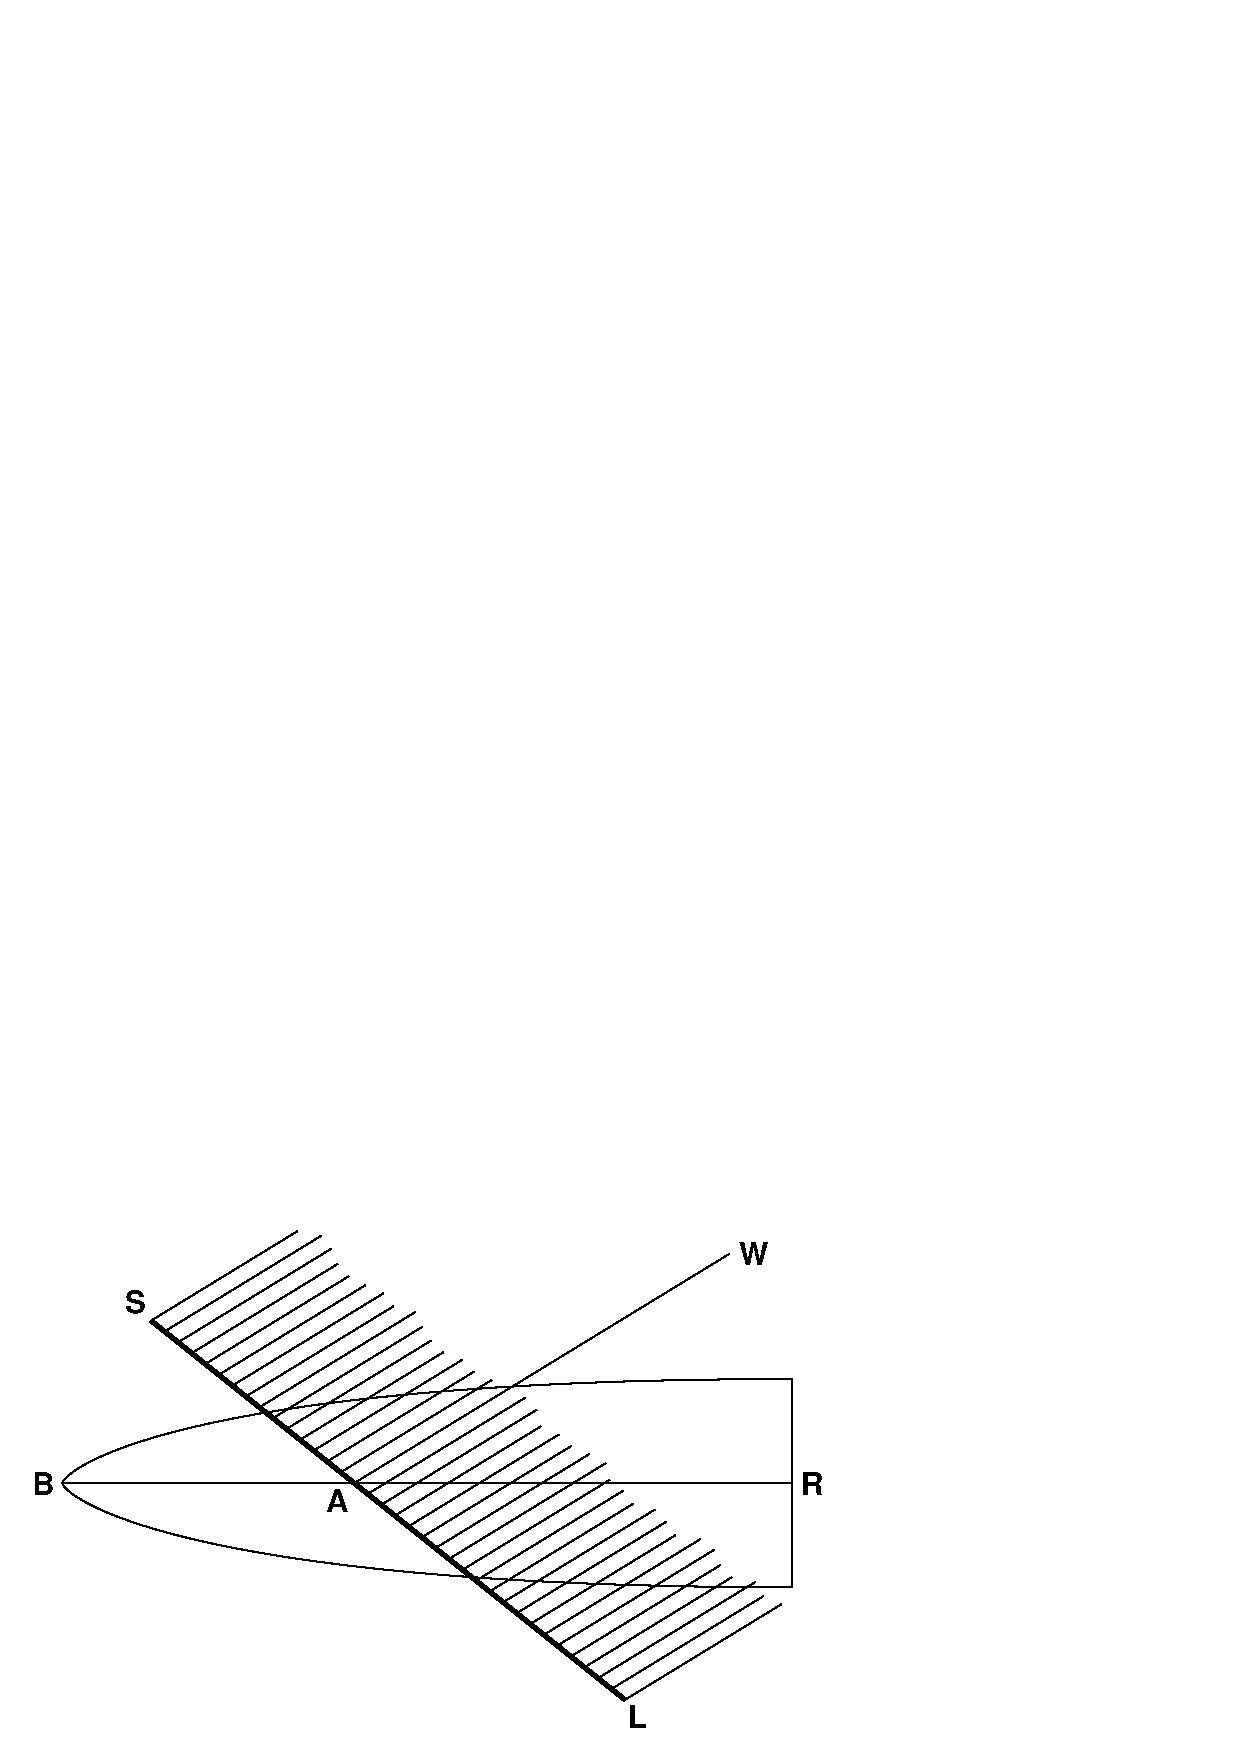
\includegraphics[width=9cm]{./images/illus110}}
\end{figure*}
to it which tends to drive the boat forwards. But as the
velocity of the boat increases, a time will arrive when the
pressure of the wind is only just able to balance the resisting
force which is caused by the sail moving through the air. The
velocity of the boat will not increase beyond this, and the
motion will be then what mathematicians describe as ``steady.''

In the accompanying figure, let $BAR$ represent the keel
of a boat, $B$ being the bow, and let $SAL$ represent the sail.
Suppose that the wind is blowing in the direction $W\!A$ with
a velocity $u$; and that this direction makes an angle $\theta$ with
\PG----File: 111.png-----------------------------------------------------
the keel, \IE\ angle $W\!AR = \theta$. Suppose that the sail is set
so as to make an angle $\alpha$ with the keel, \IE\ angle $BAS = \alpha$, and
therefore angle $W\!AL=\theta + \alpha$. Suppose finally that $v$ is the
velocity of the boat in the direction $AB$.

I have already shown that the solution of the problem
depends on the relative directions and velocities of the
wind and the boat; hence to find the result reduce the boat to
rest by impressing on it a velocity $v$ in the direction $BA$.
The resultant velocity of $v$ parallel to $BA$ and of $u$ parallel
to $W\!A$ will be parallel to $SL$, if
$v \sin \alpha = u \sin (\theta + \alpha)$; and in
this case the resultant pressure perpendicular to the sail
vanishes.

Thus, for steady motion we have $v \sin \alpha=u \sin (\theta + \alpha)$.
Hence, whenever $\sin (\theta + \alpha)>\allowbreak\sin \alpha$, we have
$v>u$. Suppose,
to take one instance, the sail to be fixed, that is, suppose $\alpha$ to
be a constant. Then $v$ is a maximum if $\theta + \alpha = \frac{1}{2}\pi$,
that is, if
$\theta$ is equal to the complement of $\alpha$. In this case we have
$v = u \cosec \alpha$, and therefore $v$ is greater than $u$. Hence, if the
wind makes the same angle $\alpha$ abaft the beam that the sail
makes with the keel, the velocity of the boat will be greater
than the velocity of the wind.

Next, suppose that the boat is running close to the wind,
so that the wind is before the beam (see figure
\vhyperlink{Figure:112}{below}),
% [**Note: original wording "on next page"]
then in the same way as before we have
$v \sin \alpha = u \sin (\theta + \alpha)$,
or $v \sin \alpha = u \sin \phi$, where
$\phi = \text{angle } W\!AS = \pi - \theta - \alpha$. Hence
$v = u \sin \phi \cosec \alpha$.

Let $w$ be the component velocity of the boat in the teeth
of the wind, that is, in the direction $AW$. Then we have
$w =\allowbreak v \cos BAW =\allowbreak v \cos (\alpha + \phi) =
\allowbreak u \sin \phi \cosec \alpha \cos (\alpha + \phi)$. If $\alpha$
is constant, this is a maximum when
$\phi = \frac{1}{4}\pi - \frac{1}{2}\alpha$; and, if $\phi$
has this value, then $w = \frac{1}{2}u (\cosec\alpha - 1)$. This formula shows
that $w$ is greater than $u$, if $\sin\alpha< \frac{1}{3}$. Thus, if the sails
can be set so that $\alpha$ is less than $\sin^{-1}\frac{1}{3}$, that is,
rather less
than $19^{\circ} 29'$, and if the wind has the direction above assigned,
then the component velocity of the boat in the face of the
wind is greater than the velocity of the wind.

\PG----File: 112.png------------------------------------------------------
The above theory is curious, but it must be remembered
that in practice considerable allowance has to be made for
the fact that no boat for use on water can be constructed in
\begin{figure*}[!hbt]
\centerline{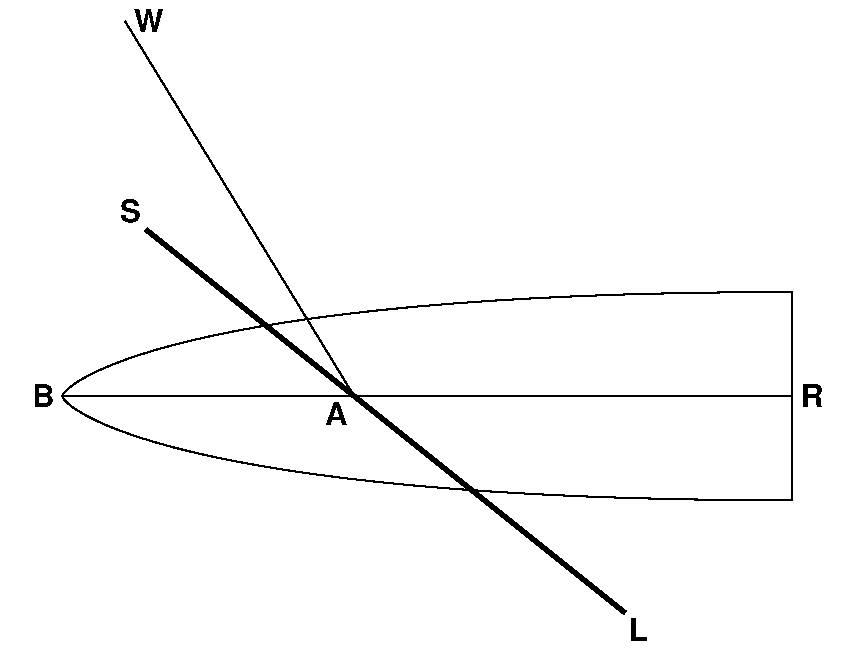
\includegraphics[width=9cm]{./images/illus112}\DPlabel{Figure:112}}
\end{figure*}
which the resistance to motion in the direction of the keel
can be wholly neglected, or which would not drift slightly to
leeward if the wind was not dead astern. Still this makes less
difference than might be thought by a landsman. In the case
of boats sailing on smooth ice the assumptions made are substantially
correct, and the practical results are said to agree
closely with the theory.

\section[Boat moved by a rope inside the boat][Boat moved by a Rope.]%
{Boat moved by a Rope} There is a form of boat-racing\index
{Boat-racing with a rope|(},
occasionally used at regattas, which affords a somewhat curious
illustration of certain mechanical principles. The only thing
supplied to the crew is a coil of rope, and they have, without
leaving the boat, to propel it from one point to another as
rapidly as possible. The motion is given by tying one end of
the rope to the after thwart, and giving the other end a series
of violent jerks in a direction parallel to the keel. I am told
that in still water a pace of two or three miles an hour can
be thus attained.

\PG----File: 113.png------------------------------------------------------
The chief cause for this result seems to be that the friction
between the boat and the water retards all relative motion,
but is not great enough to materially affect motion caused by
a sufficiently big impulse. Hence the usual movements of the
crew in the boat do not sensibly move the centre of gravity of
themselves and the boat, but this does not apply to an impulsive
movement, and if the crew in making a jerk move their
centre of gravity towards the bow $n$ times more rapidly than
it returns after the jerk, then the boat is impelled forwards
at least $n$ times more than backwards: hence on the whole
the motion is forwards\index
{Boat-racing with a rope|)}\index{Sailing@\textsc{Sailing}, Theory of|)}.

\section[Results dependent on Hauksbee's Law][Motion of Fluids.]%
{Motion of Fluids and Motion in Fluids} The theories
of \emph{motion of fluids}\index{Fluid Motion|(} and
\emph{motion in fluids}\index{Motion in Fluids|(} involve considerable
difficulties. Here I will mention only one or two instances---mainly
illustrations of Hauksbee's Law.

\subsection*{Hauksbee's Law} When a fluid is in rapid motion\index
{Hauksbee@\textsc{Hauksbee's Law}|(} the
pressure is less than when it is at rest\footnote
{See Besant\index{Besant on Hauksbee's Law}, \textit{Hydromechanics},
Cambridge, 1867, art.~149, where however
it is assumed that the pressure is proportional to the density.
Hauksbee was the earliest writer who called attention to the problem,
but I do not know who first explained the phenomenon; some references
to it are given by Willis\index{Willis on Hauksbee's law},
\textit{Cambridge Philosophical Transactions}, 1830,
vol.~\textsc{iii}, pp.~129--140.}. Thus, if a current
of air is moving in a tube, the pressure on the sides of the
tube is less than when the air is at rest---and the quicker the
air moves the smaller is the pressure. This fact was noticed
by Hauksbee nearly two centuries ago. In an elastic perfect
fluid in which the pressure is proportional to the density, the
law connecting the pressure, $p$, and the steady velocity, $v$, is
$p = \Pi\alpha^{-v^2}$ where $\Pi$ and $\alpha$ are constants: the
establishment of
corresponding formula for gases where the pressure is proportional
to a power of the density presents no difficulty.

This principle is illustrated by a twopenny toy, on sale in
most toy-shops, called the \emph{pneumatic mystery}. It consists of a
tube, with a cup-shaped end in which rests a wooden ball. If
the tube is held in a vertical position, with the mouthpiece at
\PG----File: 114.png-------------------------------------------------------
the upper end and the cup at the lower end, then, if anyone
blows hard through the tube and places the ball against the
cup, the ball will remain suspended there. The explanation is
that the pressure of the air below the ball is so much greater
than the pressure of the air in the cup that the ball is held up.

The same effect may be produced by fastening to one end
of a tube a piece of cardboard having a small hole in it. If
a piece of paper is placed over the hole and the experimenter
blows through the tube, the paper will not be detached from
the card but will bend so as to allow the egress of the air.

An exactly similar experiment, described in many text-books
on hydromechanics, is made as follows. To one end of a
straight tube a plane disc is fitted which is capable of sliding
on wires projecting from the end of the tube. If the disc is
placed at a small distance from the end, and anyone blows
steadily into the tube, the disc will be drawn towards the tube
instead of being blown off the wires, and will oscillate about a
position near the end of the tube.

In the same way we may make a tube by placing two books
on a table with their backs parallel and an inch or so apart and
laying a sheet of newspaper over them. If anyone blows
steadily through the tube so formed, the paper will be sucked in
instead of being blown out.

The following experiment is explicable by the same argument.
On the top of a vertical axis balance a thin horizontal
rod. At each end of this rod fasten a small vertical square or
sail of thin cardboard---the two sails being in the same plane.
If anyone blows close to one of these squares and in a direction
parallel to its plane, the square will move towards the side on
which one is blowing, and the rod with the two sails will
rotate about the axis.

The experiments above described can be performed so as
to illustrate Hauksbee's Law; but unless care is taken other
causes will be also introduced which affect the phenomena:
it is however unnecessary for my purpose to go into these
details.
\PG----File: 115.png-------------------------------------------------------

\subsection[Cut on a tennis-ball. \texorpdfstring{\protect\quad}{} Spin on a cricket-ball]%
[Spin on Tennis and Cricket Balls.]{Cut on a Tennis-Ball}
Racquet and tennis players know
that if a strong cut is given to a ball it can be made to%
\index{Cut on a Tennis-ball|(}%
\index{Racquet-ball, Cut on|(}%
\index{Tennis-ball, Cut on|(}
rebound off a vertical wall and then (without striking the
floor or any other wall) return and hit the wall again.

This affords another illustration of Hauksbee's Law. The
explanation\footnote
{See Magnus\index{Magnus on Hauksbee's Law} on
`\textit{Die Abweichung der Geschosse}' in the \textit{Abhandlungen
der Akademie der Wissenschaften}, Berlin, 1852, pp.~1--23;
Lord Rayleigh\index{Rayleigh},
`\textit{On the irregular flight of a tennis ball},'
\textit{Messenger of Mathematics},
Cambridge, 1878, vol.~\textsc{vii}, pp.~14--16.
} is that the cut causes the ball to rotate rapidly
about an axis through its centre of figure, and the friction of the
surface of the ball on the air produces a sort of whirlpool. This
rotation is in addition to its motion of translation. Suppose the
ball to be spherical and rotating about an axis through its centre
perpendicular to the plane of the paper in the direction of the
arrow-head, and at the same time moving through still air from
left to right parallel to $PQ$. Any motion of the ball perpendicular
to $PQ$ will be produced by the pressure of the air on the
surface of the ball, and this pressure will, by Hauksbee's Law,
be greatest where the velocity of the air relative to the ball is
least, and vice versa. To find the velocity of the air relative
to the ball we may reduce the centre of the ball to rest, and
suppose a stream of air to impinge on the surface of the ball
moving with a velocity equal and opposite to that of the
centre of the ball. The air is not frictionless, and therefore
the air in contact with the surface of the ball will be set in
motion, by the rotation of the ball and will form a sort of
whirlpool rotating in the direction of the arrow-head in the
figure. To find the actual velocity of this air relative to the
ball we must consider how the motion due to the whirlpool is
affected by the motion of the stream of air parallel to $QP$.
The air at $A$ in the whirlpool is moving against the stream of
air there, and therefore its velocity is retarded: the air at $B$
in the whirlpool is moving in the same direction as the stream
of air there, and therefore its velocity is increased. Hence the
relative velocity of the air at $A$ is less than that at $B$, and
\PG----File: 116.png-------------------------------------------------------
since the pressure of the air is greatest where the velocity is
least, the pressure of the air on the surface of the ball at $A$ is
greater than on that at $B$, Hence the ball is forced by this
\begin{figure*}[!hbt]
\centerline{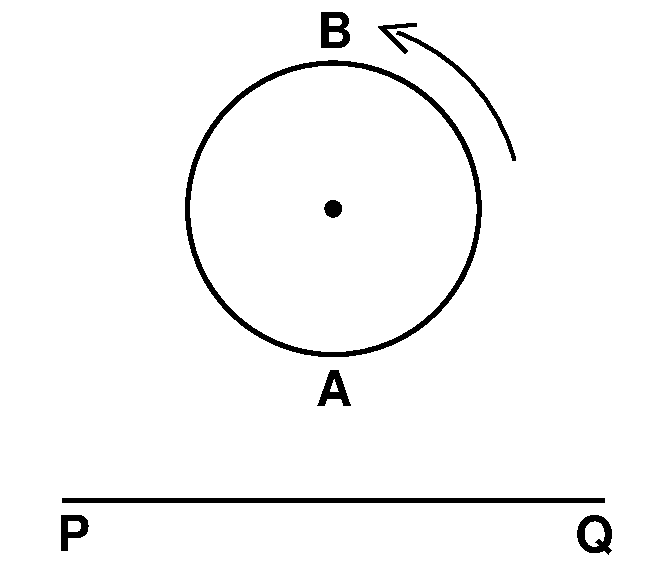
\includegraphics[height=\ifPaper3.5cm\else5cm\fi]{./images/illus116}}
\end{figure*}
pressure in the direction from the line $PQ$, which we may
suppose to represent the section of the vertical wall in a
racquet-court. In other words, the ball tends to move at right
angles to the line in which its centre is moving and in the
direction in which the surface of the front of the ball is being
carried by the rotation\index{Hauksbee@\textsc{Hauksbee's Law}|)}.

In the case of a lawn tennis-ball, the shape of the ball is
altered by a strong cut, and this introduces additional complications%
\index{Cut on a Tennis-ball|)}%
\index{Racquet-ball, Cut on|)}%
\index{Tennis-ball, Cut on|)}.

\subsection*{Spin on a Cricket-Ball} The curl of a cricket-ball%
\index{Spin on Cricket-ball}\index{Cricket-Ball, Spin on} in its
flight through the air, caused by a spin given by the bowler in
delivering the ball, is explained by the same reasoning.

Thus suppose the ball is delivered in a direction lying in a
vertical plane containing the two middle stumps of the wickets.
A spin round a horizontal axis parallel to the crease in a
direction which the bowler's umpire would describe as positive,
namely, counter clock-wise, will, in consequence of the friction
of the air, cause it to drop, and therefore decrease the length
of the pitch. A spin in the opposite direction will cause it to
rise, and therefore lengthen the pitch. A spin round a vertical
axis in the positive direction, as viewed from above, will make
it curl sideways in the air to the left, that is, from leg to off.
A spin in the opposite direction will make it curl to the right.
A spin given to the ball round the direction of motion of the
\PG----File: 117.png--------------------------------------------------
centre of the ball will not sensibly affect the motion through
the air, though it would cause the ball, on hitting the ground,
to break. Of course these various kinds of spin can be
combined.

\ThoughtBreakSpace
The questions involving the application of Hauksbee's Law
are easy as compared with many of the problems in fluid
motion. The analysis required to attack most of these problems
is beyond the scope of this book, but one of them may
be worth mentioning even though no explanation is given.

\subsection*{The Theory of the Flight of Birds}%
\addcontentsline{toc}{section}{Flight of Birds}%
\markright{Flight of Birds.}%
A mechanical problem\index{Birds, Flight of|(}
of great interest is the explanation of the means by which
birds are enabled to fly for considerable distances with no
(perceptible) motion of the wings. Albatrosses, to take an
instance of special difficulty, have been known to follow for
some days ships running at the rate of nine or ten knots, and
sometimes for considerable periods there is no motion of the
wings or body which can be detected, while even if the bird
moved its wings it is not easy to understand how it has the
muscular energy to propel itself so rapidly and for such a length
of time. Of this phenomenon various explanations\footnote
{See G.H.~Bryan\index{Bryan on Bird Flight} in the
\textit{Transactions of the British Association} for
1896, vol.~\textsc{lxvi}, pp.~726-728.} have
been suggested. Notable among these are Mr~Maxim's\index
{Maxim on Bird Flight} of
upward air-currents, Lord Rayleigh's\index{Rayleigh} of variations of the
wind velocity at different heights above the ground, Dr~S.P.~Langley's\index
{Langley on Bird Flight}
of the incessant occurrence of gusts of wind separated by lulls,
and Dr~Bryan's of vortices in the atmosphere.

It now seems reasonably certain that the second and third of
these sources of energy account for at least a portion of the
observed phenomena. The effect of the third cause may be
partially explained by noting that the centre of gravity of the
bird with extended wings is slightly below the aeroplane or wing
surface, so that the animal forms a sort of parachute. The effect
of a sudden gust of wind upon such a body is that the aeroplane
is set in motion more rapidly than the suspended mass, causing
\PG----File: 118.png------------------------------------------------------
the structure to heel over so as to receive the wind on the under
surface of the aeroplane, and this lifts the suspended mass
giving it an upward velocity. When the wind falls the greater
inertia of the mass carries it on upwards causing the aeroplane
to again present its under side to the air; and if while the
parachute is in this position the wind is still blowing from the
side, the suspended mass is again lifted. Thus the more the
bird is blown about, the more it rises in the air; actually birds
in flight are carried up by a sudden side gust of wind as we
should expect from this theory.

The fact that the bird is in motion tends also to keep it up,
for it has been recently shown that a horizontal plane under
the action of gravity falls to the ground more slowly if it is
travelling through the air with horizontal velocity than it
would do if allowed to fall vertically, hence the bird's forward
motion causes it to fall through a smaller height between
successive gusts of wind than it would do if it were at rest,
Moreover it has been proved experimentally that the horsepower
required to support a body in horizontal flight by means
of an aeroplane is less for high than for low speeds: hence
when a side-wind (that is, a wind at right angles to the bird's
course) strikes the bird, the lift is increased in consequence
of the bird's forward velocity\index{Birds, Flight of|)}\index
{Fluid Motion|)}\index{Motion in Fluids|)}.

\section{Curiosa Physica} When I was writing the first edition\index
{Curiosa Physica|(}
of these ``Recreations,'' I put together a chapter, following
this one, on ``Some Physical Questions,'' dealing with problems
such as, in the Theory of Sound\index
{Sound, Problem in}, the explanation of the
fact that in some of Captain Parry's\index
{Parry on Sound} experiments the report
of a cannon\index{Gun, Report of}, when fired, travelled so much more rapidly
than the sound of the human voice that observers heard the
report of the cannon when fired before that of the order to
fire it\footnote
{The fact is well authenticated. Mr~Earnshaw\index{Earnshaw, S.}
(\textit{Philosophical Transactions}, London, 1860, pp.~133--148)
explained it by the acceleration of
a wave caused by the formation of a kind of bore, a view accepted
by Clerk Maxwell and most physicists, but Sir George Airy\index
{Airy, Sir Geo.} thought that the
explanation was to be found in physiology; see Airy's \textit{Sound}, second
edition, London, 1871, pp.~141, 142.
}: in the Kinetic Theory of Gases, the complications in
\PG----File: 119.png------------------------------------------------------
our universe that might be produced by ``Maxwell's demon''\index
{Maxwell's Demon}\footnote
{See \textit{Theory of Heat}, by J.~Clerk Maxwell\index{Maxwell, J. Clerk},
second edition, London, 1872, p.~308.}:
in the Theory of Optics, the explanation of the Japanese\index
{Japanese Magic Mirrors}\index{Magic Mirrors}\index{Mirrors, Magic}
``magic mirrors,''\footnote
{See a memoir by W.E.~Ayrton\index{Ayrton on Magic Mirrors} and J.~Perry\index
{Perry on Magic Mirrors}, \textit{Proceedings of the
Royal Society of London}, part~\textsc{i}, 1879, vol.~\textsc{xxviii},
pp.~127--148.}
which reflect the pattern on the back of
the mirror (on which the light does not fall): to which I
might add the theory of the ``spectrum top\index{Spectrum Top},'' by means
of which a white surface, on which some black lines are
drawn, can be moved so as to give the impression\footnote
{See letters from Mr~C.E.~Benham\index{Benham on Spectrum Top} and others in
\textit{Nature}, 1894--5;
and a memoir by Prof.\ Liveing\index{Liveing on the Spectrum Top},
Cambridge Philosophical Society, November~26, 1894.} that the
lines are coloured (red, green, blue, slate, or drab), and the
curious fact that the colours change with the direction of
rotation: it has also been recently shown that if two trains
of waves, whose lengths are in the ratio $m-1: m+1$, be
superposed\index{Waves, Superposition of}, then every $m$th wave in the
system will be big---thus
the current opinion that every ninth wave in the open
sea is bigger than the other waves may receive scientific
confirmation. There is no lack of interesting and curious
phenomena in physics, and in some branches, notably in
electricity and magnetism, the difficulty is rather one of selection,
but I felt that the connection with mathematics was in
general either too remote or too technical to justify the insertion
of such a collection in a work on elementary mathematical
recreations, and therefore I struck out the chapter. I
mention the fact now partly to express the hope that some
physicist will one day give us a collection of the kind, partly
to suggest these questions to those who are interested in such
matters\index{Curiosa Physica|)}.

\PG----File: 120.png------------------------------------------------------
% CHAPTER IV.

\chapter[Some Miscellaneous Questions.]%
[Miscellaneous Mathematical Recreations.]{Some Miscellaneous Questions.}

\textsc{I propose} to discuss in this chapter the mathematical theory
of certain of the more common mathematical amusements and
games. Some of these might have been treated in the first
two chapters, but, since most of them involve mixed geometry
and algebra, it is rather more convenient to deal with
them apart from the problems and puzzles which have been
described already. This division, however, is by no means well
defined, and the arrangement is based on convenience rather
than on any logical distinction.

The majority of the questions here enumerated have no
connection one with another, and I jot them down almost at
random.

I shall discuss in succession the \emph{Fifteen Puzzle}, the \emph{Tower
of Hanoï}, \emph{Chinese Rings}, the \emph{Eight Queens Problem}, the
\emph{Fifteen School-Girls Problem}, and some miscellaneous \emph
{Problems connected with a pack of cards}.

\ssection[The Fifteen Puzzle]{The Fifteen Puzzle\protect\footnote
{There are two articles on the subject in the \textit{American Journal of
Mathematics} 1879, vol.~\textsc{ii}, by Professors Woolsey Johnson\index
{Johnson on Fifteen Puzzle} and Story\index{Story on the Fifteen Puzzle};
but the whole theory is deducible immediately from the proposition I
give above in the text.}}
Some years ago the so-called
\emph{fifteen puzzle}\index{Fifteen@\textsc{Fifteen Puzzle}|(} was on sale
in all toy-shops. It consists of a
shallow wooden box---one side being marked as the top---in the
form of a square, and contains fifteen square blocks or counters
\PG----File: 121.png-------------------------------------------------------
numbered $1$, $2$, $3 \ldots$ up to $15$. The box will hold just sixteen
such counters, and, as it contains only fifteen, they can be
moved about in the box relatively to one another. Initially
they are put in the box in any order, but leaving the sixteenth
cell or small square empty; the puzzle is to move them so
that finally they occupy the position shown in the first of the
annexed figures.

\begin{figure*}[!hbt]
\centering
\ifPaper\else\hspace*{\fill}\fi
\begin{minipage}{\ifPaper0.45\textwidth\else0.33\textwidth\fi}
\centerline{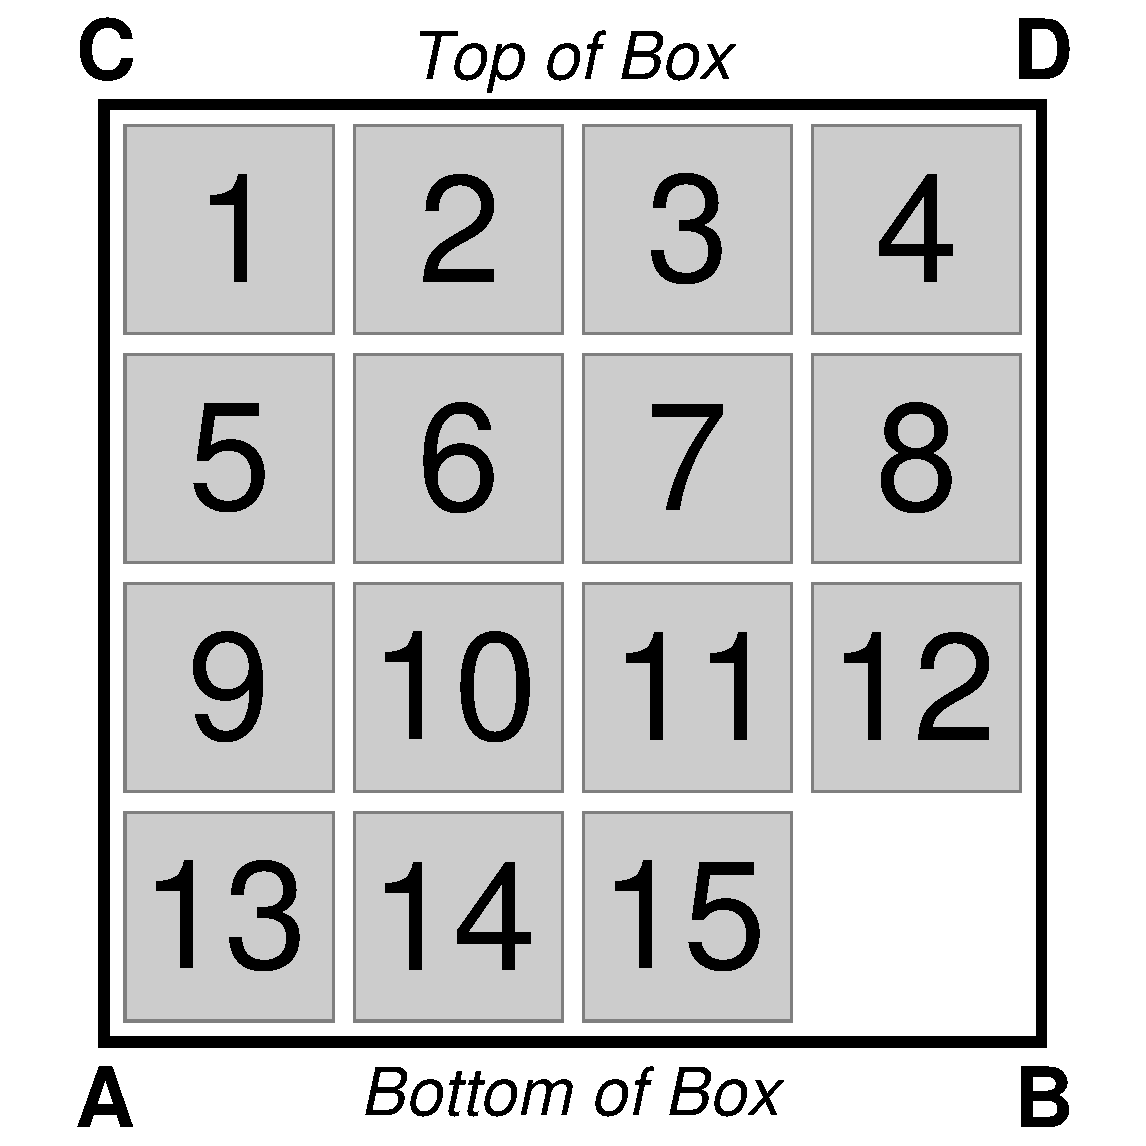
\includegraphics[width=\textwidth]{./images/illus121a}}
\end{minipage}
\hfill
\begin{minipage}{\ifPaper0.45\textwidth\else0.33\textwidth\fi}
\centerline{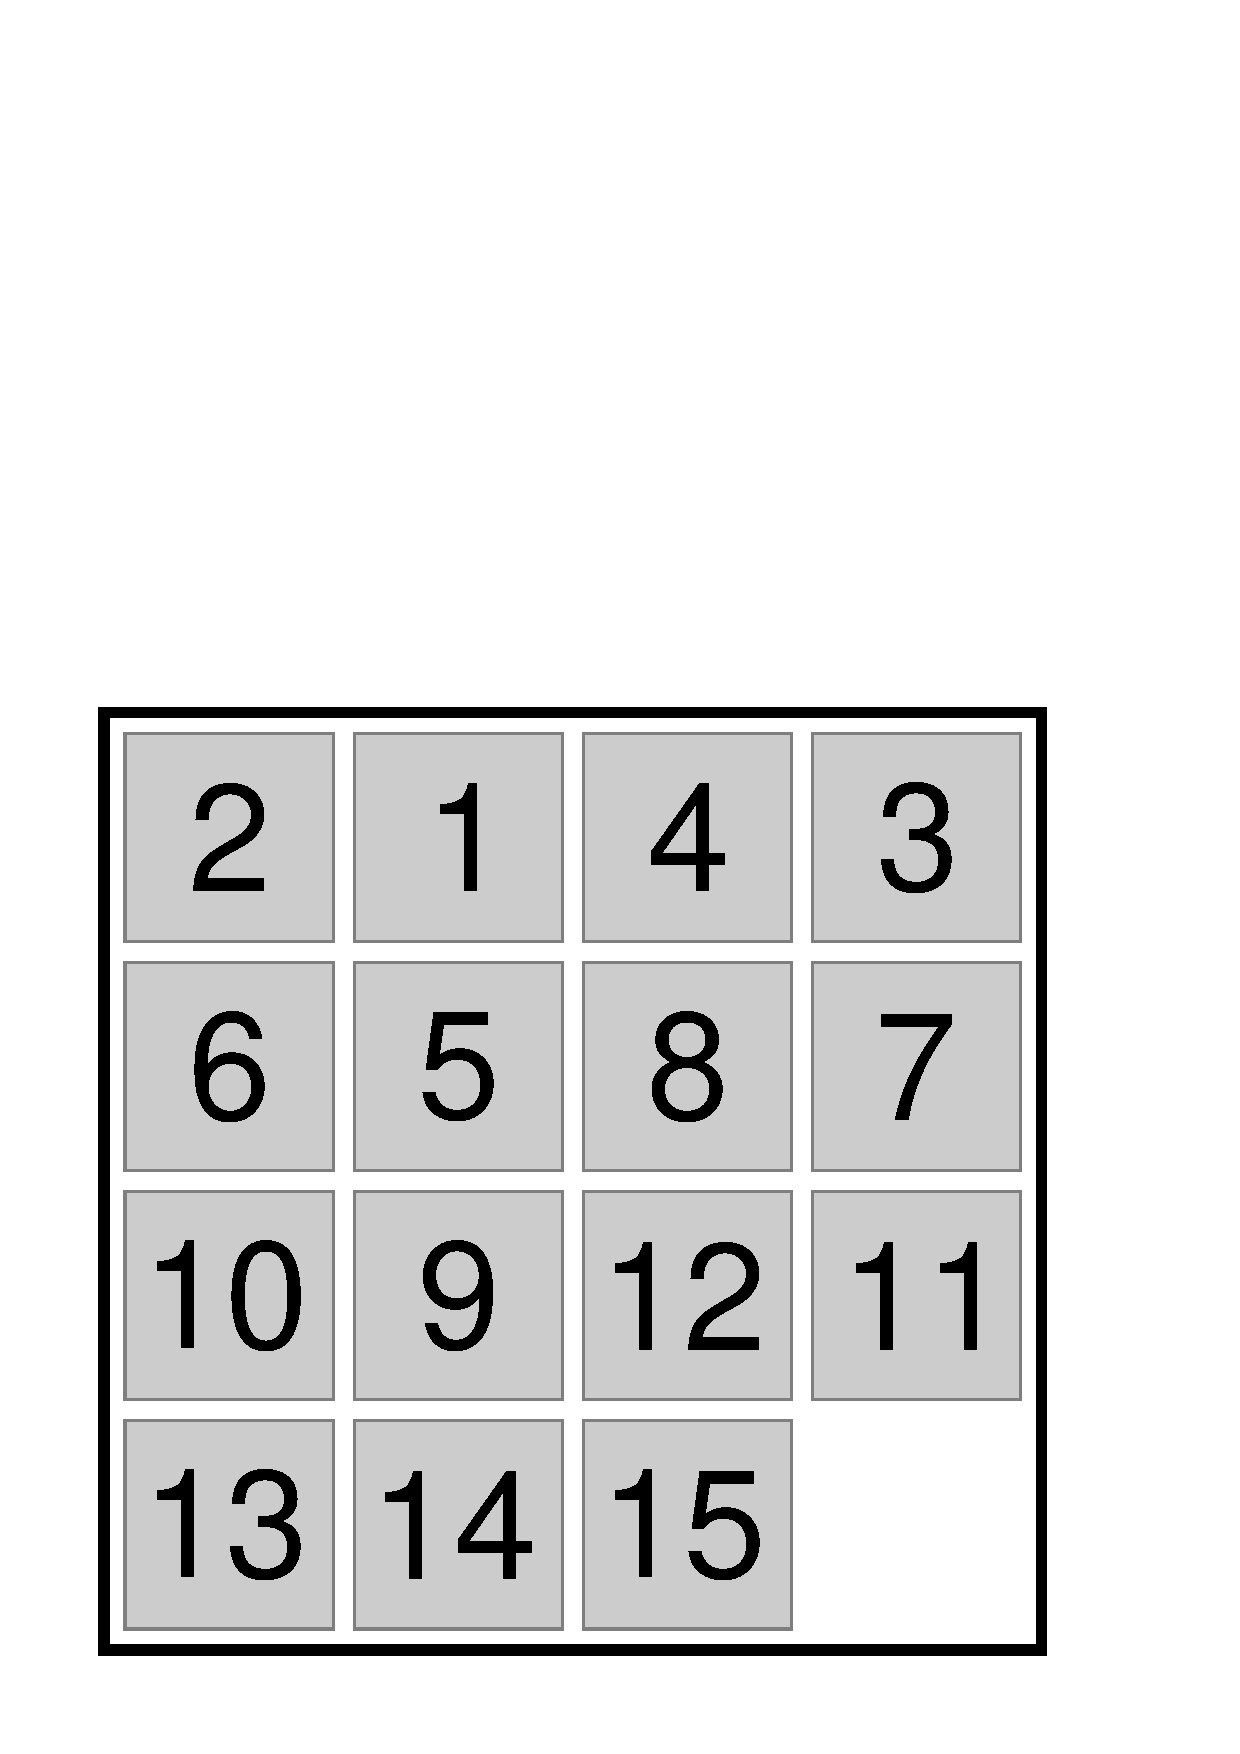
\includegraphics[width=\textwidth]{./images/illus121b}}
\end{minipage}
\ifPaper\else\hspace*{\fill}\fi
\label{illus:121}
\end{figure*}

We may represent the various stages in the game by supposing
that the blank space, occupying the sixteenth cell, is
moved over the board, ending finally where it started.

The route pursued by the blank space may consist partly of
tracks followed and again retraced, which have no effect on the
arrangement, and partly of closed paths travelled round, which
necessarily are cyclical permutations of an odd number of
counters. No other motion is possible.

Now a cyclical permutation of $n$ letters is equivalent to
$n-1$ simple interchanges; accordingly an odd cyclical permutation
is equivalent to an even number of simple interchanges.
Hence, if we move the counters so as to bring the blank space
back into the sixteenth cell, the new order must differ from
the initial order by an even number of simple interchanges. If
\PG----File: 122.png-------------------------------------------------------
therefore the order we want to get can be obtained from this
initial order only by an odd number of interchanges, the
problem is incapable of solution; if it can be obtained by an
even number, the problem is possible.

Thus the order in the second of the diagrams given
\vpageref{illus:121}
%[**Note: original wording "on the opposite page"
is deducible from that in the first diagram by six
interchanges; namely, by interchanging the counters $1$ and $2$, $3$
and $4$, $5$ and $6$, $7$ and $8$, $9$ and $10$, $11$ and $12$. Hence the one
can be deduced from the other by moving the counters about in the box.

If however in the second diagram the order of the last
three counters had been $13$, $15$, $14$, then it would have required
seven interchanges of counters to bring them into the order
given in the first diagram. Hence in this case the problem
would be insoluble.

{\renewcommand\tabcolsep{4pt} % for several tabulars
The easiest way of finding the number of simple interchanges
necessary in order to obtain one given arrangement
from another is to make the transformation by a series of
cycles. For example, suppose that we take the counters in
the box in any definite order, such as taking the successive
rows from left to right, and suppose the original order and the
final order to be respectively
\[
\begin{tabularx}{\textwidth}{@{}X@{}rrrrrrrrrrrrrrr@{}X@{}}
& $1$,  & $13$, & $2$, & $3$, & $5$, & $7$, & $12$, & $8$, &
 $15$, & $6$, & $9$,  & $4$,  & $11$, & $10$, & $14$,&\\
and& $11$, & $2$,  & $3$, & $4$, & $5$, & $6$, & $7$,  &
 $1$, & $9$,  &$10$, & $13$, & $12$, & $8$,  & $14$, & $15$.&
\end{tabularx}
\]
We can deduce the second order from the first by $12$ simple
interchanges. The simplest way of seeing this is to arrange the
process in three separate cycles as follows:---
\[
\begin{tabular}
{rrr@{\hglue8pt}|@{\hglue8pt}rrrrrrrrrrr@{\hglue8pt}|@{\hglue8pt}r}
$1$,  & $11$, & $8\;$; & $13$, & $2$, & $3$, & $4$,  & $12$, & $7$, &
 $6$,  & $10$, & $14$, & $15$, & $9\;$;  & $5$. \\
$11$, & $8$,  & $1\;$; & $2$,  & $3$, & $4$, & $12$, & $7$,  & $6$, &
 $10$, & $14$, & $15$, & $9$,  & $13\;$; & $5$.
\end{tabular}
\]
Thus, if in the first row of figures $11$ is substituted for $1$, then
$8$ for $11$, then $1$ for $8$, we have made a cyclical interchange of
$3$ numbers, which is equivalent to $2$ simple interchanges (namely,
interchanging $1$ and $11$, and then $1$ and $8$). Thus the whole
process is equivalent to one cyclical interchange of $3$ numbers,
another of $11$ numbers, and another of $1$ number. Hence it is
\PG----File: 123.png-------------------------------------------------------
equivalent to $(2 + 10 + 0)$ simple interchanges. This is an even
number, and thus one of these orders can be deduced from the
other by moving the counters about in the box.

It is obvious that, if the initial order is the same as the
required order except that the last three counters are in the
order $15$, $14$, $13$, it would require one interchange to put them
in the order $13$, $14$, $15$; hence the problem is insoluble.

If however the box is turned through a right angle, so as
to make $AD$ the top, this rotation will be equivalent to $13$
simple interchanges. For, if we keep the sixteenth square
always blank, then such a rotation would change any order
such as
\[
\begin{tabularx}{\textwidth}{@{}X@{}rrrrrrrrrrrrrrr@{}X@{}}
 & $1$,  & $2$, & $3$, & $4$, &  $5$,  & $6$,  & $7$, & $8$, & $9$,  &
 $10$, & $11$, & $12$, & $13$, & $14$, & $15$,&\\
to & $13$, & $9$, & $5$, & $1$, &  $14$, & $10$, & $6$, & $2$, & $15$, &
 $11$, & $7$,  & $3$,  & $12$, & $8$,  & $4$,&
\end{tabularx}
\]
which is equivalent to $13$ simple interchanges. Hence it will
change the arrangement from one in which a solution is impossible
to one where it is possible, and vice versa.

Again, even if the initial order is one which makes a solution
impossible, yet if the first cell and not the last is left
blank it will be possible to arrange the fifteen counters in
their natural order. For, if we represent the blank cell by $b$,
this will be equivalent to changing the order
\[
\begin{tabular}{rrrrrrrrrrrrrrrr}
$1$, & $2$, & $3$, & $4$, & $5$, & $6$, & $7$, & $8$, & $9$, & $10$, &
 $11$, & $12$, & $13$, & $14$, & $15$, & $b$, \\
$b$, &$1$,  & $2$, & $3$, & $4$, & $5$, & $6$, & $7$, & $8$, & $9$,  &
 $10$, & $11$, & $12$, & $13$, & $14$, & $15$\phantom{,}\rlap{$\;$:}
\end{tabular}
\]
this is a cyclical interchange of $16$ things and therefore is
equivalent to $15$ simple interchanges. Hence it will change
the arrangement from one in which a solution is impossible to
one where it is possible, and vice versa.}

It is evident that the above principles are applicable
equally to a rectangular box containing $mn$ cells or spaces and
$mn-1$ counters which are numbered. Of course $m$ may be
equal to $n$. If such a box is turned through a right angle, and
$m$ and $n$ are both even, it will be equivalent to $mn-3$ simple
interchanges---and thus will change an impossible position to
a possible one, and vice versa---but unless both $m$ and $n$ are
\PG----File: 124.png---------------------------------------------------------
even the rotation is equivalent to only an even number of
interchanges. Similarly, if either $m$ or $n$ is even, and it is
impossible to solve the problem when the last cell is left blank,
then it will be possible to solve it by leaving the first cell
blank.

The problem may be made more difficult by limiting the
possible movements by fixing bars inside the box which will
prevent the movement of a counter transverse to their directions.
We can conceive also of a similar cubical puzzle, but
we could not work it practically except by sections\index
{Fifteen@\textsc{Fifteen Puzzle}|)}.


\section{The Tower of Hanoï} I may mention next the ingenious%
\index{Hanoi@\textsc{Hanoï, Tower of}|(}%
\index{Tower@\textsc{Tower of Hanoï}|(}
puzzle known as the \emph{Tower of Hanoï}. It was brought out in
1883 by M.~Claus\index{Claus} (Lucas\index{Lucas, E.}).

It consists of three pegs fastened to a stand, and of
eight circular discs of wood or cardboard each of which has
a hole in the middle so that a peg can be put through it.
These discs are of different radii, and initially they are placed
all on one peg, so that the biggest is at the bottom, and the
radii of the successive discs decrease as we ascend: thus the
smallest disc is at the top. This arrangement is called the
\emph{Tower}. The problem is to shift the discs from one peg to
another in such a way that a disc shall never rest on one
smaller than itself, and finally to transfer the tower (\IE\ all
the discs in their proper order) from the peg on which they
initially rested to one of the other pegs.

The method of effecting this is as follows. (i)~If initially
there are $n$ discs on the peg $A$, the first operation is to transfer
gradually the top $n-1$ discs from the peg $A$ to the peg $B$,
leaving the peg $C$ vacant: suppose that this requires $x$ separate
transfers. (ii)~Next, move the bottom disc to the peg $C$.
(iii)~Then, reversing the first process, transfer gradually the
$n-1$ discs from $B$ to $C$, which will necessitate $x$ transfers.
Hence, if it requires $x$ transfers of simple discs to move a
tower of $n-1$ discs, then it will require $2x +1$ separate
transfers of single discs to move a tower of $n$ discs. Now
\PG----File: 125.png---------------------------------------------------------
with $2$ discs it requires $3$ transfers, \IE\ $2^2-1$ transfers;
hence with $3$ discs the number of transfers required will be
$2 (2^2-1) + 1$, that is, $2^3-1$. Proceeding in this way we see
that with a tower of $n$ discs it will require $2^n-1$ transfers
of single discs to effect the complete transfer. Thus the eight
discs of the puzzle will require $255$ single transfers. The result
can be also obtained by the theory of finite differences. It
will be noticed that every alternate move consists of a transfer
of the smallest disc from one peg to another, the pegs being
taken in cyclical order.

M.~De~Parville\index{DeParville@De Parville on Tower of Hanoï}\index
{Parville@Parville on Tower of Hanoï} gives an account of the origin
of the toy
which is a sufficiently pretty conceit to deserve repetition\footnote
{\textit{La Nature}, Paris, 1884, part~\textsc{i}, pp.~285--286.}.
In the great temple at Benares, says he, beneath the dome
which marks the centre of the world, rests a brass-plate in
which are fixed three diamond needles, each a cubit high
and as thick as the body of a bee. On one of these needles,
at the creation, God placed sixty-four discs of pure gold, the
largest disc resting on the brass plate, and the others getting
smaller and smaller up to the top one. This is the Tower of
Bramah. Day and night unceasingly the priests transfer the
discs from one diamond needle to another according to the
fixed and immutable laws of Bramah, which require that the
priest must not move more than one disc at a time and that
he must place this disc on a needle so that there is no smaller
disc below it. When the sixty-four discs shall have been thus
transferred from the needle on which at the creation God
placed them to one of the other needles, tower, temple, and
Brahmins alike will crumble into dust, and with a thunder-clap
the world will vanish. Would that English writers were
in the habit of inventing equally interesting origins for the
puzzles they produce!

The number of separate transfers of single discs which the
Brahmins must make to effect the transfer of the tower is
$2^{64}-1$, that is, is $18,446744,073709,551615$: a number which,
\PG----File: 126.png---------------------------------------------------------
even if the priests never made a mistake, would require many
thousands of millions of years to carry out%
\index{Hanoi@\textsc{Hanoï, Tower of}|)}%
\index{Tower@\textsc{Tower of Hanoï}|)}.

\section[Chinese Rings]{Chinese Rings\protect\footnote
{It was described by Cardan\index{Cardan} in 1550 in his \textit
{De Subtilitate}, bk.~\textsc{xv},
paragr.~2, ed.\ Sponius, vol.~\textsc{iii}, p.~587; by Wallis\index
{Wallis, J.} in his \textit{Algebra}, second
edition, 1693, \textit{Opera}, vol.~\textsc{ii}, chap.~111, pp.~472--478;
and allusion is
made to it also in Ozanam's\index{Ozanam@Ozanam's \textit{Récréations}}
\textit{Récréations}, 1723 edition, vol.~\textsc{iv}, p.~439.
}} A somewhat more elaborate toy, known\index
{Chinese rings@\textsc{Chinese rings}|(}
as \emph{Chinese Rings}, which is on sale in most English toy-shops,
is represented in the accompanying figure. It consists of a
\begin{figure*}[!hbt]
\centerline{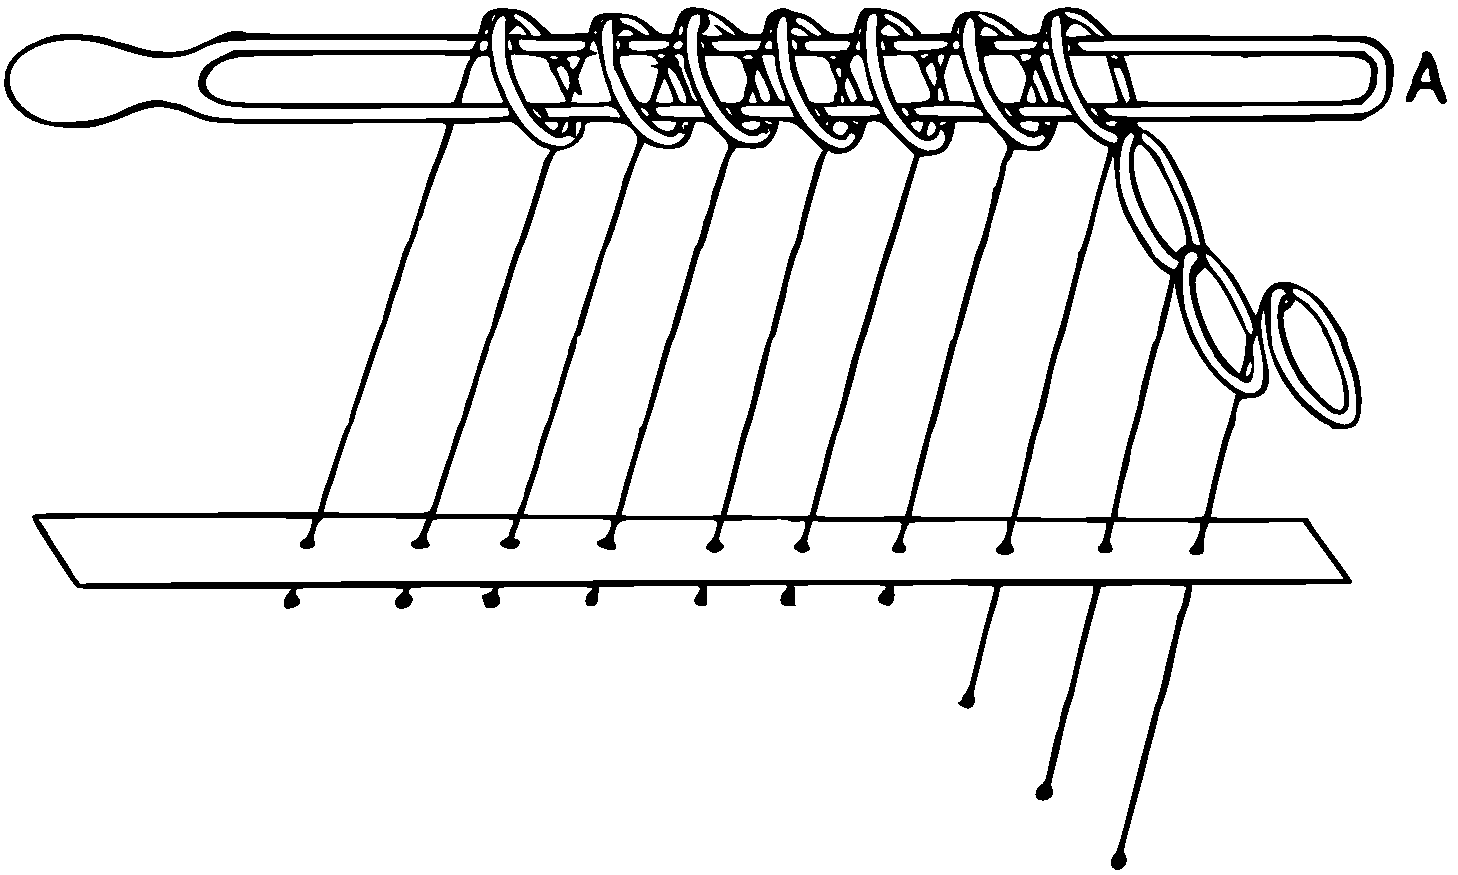
\includegraphics[width=11.5cm]{./images/illus126}}
\end{figure*}
number of rings hung upon a bar in such a manner that the
ring at one end (say $A$) can be taken off or put on the bar
at pleasure; but any other ring can be taken off or put on
only when the one next to it towards $A$ is on, and all the
rest towards $A$ are off the bar. The order of the rings cannot
be changed.

Only one ring can be taken off or put on at a time. [In
the toy, as usually sold, the first two rings form an exception
to the rule. Both these can be taken off or put on together.
To simplify the discussion I shall assume at first that only
one ring is taken off or put on at a time.] I proceed to show
that, if there are $n$ rings, then in order to disconnect them
\PG----File: 127.png---------------------------------------------------------
from the bar, it will be necessary to take a ring off or to
put a ring on either $\frac{1}{3}(2^{n+1}-1)$ times or
$\frac{1}{3}(2^{n+1}-2)$ times according as $n$ is odd or even.

Let the taking a ring off the bar or putting a ring on the
bar be called a \emph{step}. It is usual to number the rings from the
free end $A$. Let us suppose that we commence with the first
$m$ rings off the bar and all the rest on the bar; and suppose
that then it requires $x-1$ steps to take off the next ring,
that is, it requires $x-1$ additional steps to arrange the rings
so that the first $m + 1$ of them are off the bar and all the
rest are on it. Before taking these steps we can take off the
$(m + 2)$th ring and thus it will require $x$ steps from our initial
position to remove the $(m + 1)$th and $(m + 2)$th rings.

Suppose that these $x$ steps have been made and that thus
the first $m + 2$ rings are off the bar and the rest on it, and
let us find how many additional steps are now necessary to
take off the $(m + 3)$th and $(m + 4)$th rings. To take these
off we begin by taking off the $(m + 4)$th ring: this requires
$1$ step. Before we can take off the $(m + 3)$th we must arrange
the rings so that the $(m + 2)$th is on and the first $m + 1$ rings
are off: to effect this, (i)~we must get the $(m + 1)$th ring on
and the first $m$ rings off, which requires $x-1$ steps, (ii)~then
we must put on the $(m + 2)$th ring, which requires $1$ step,
(iii)~and lastly we must take the $(m + 1)$th ring off, which
requires $x-1$ steps: thus this series of movements requires in
all $\{2 (x-1) + 1\}$ steps. Next we can take the $(m + 3)$th ring
off, which requires $1$ step; this leaves us with the first $m + 1$
rings off, the $(m + 2)$th on, the $(m + 3)$th off and all the rest on.
Finally to take off the $(m + 2)$th ring, (i)~we get the $(m + 1)$th
ring on and the first $m$ rings off, which requires $x-1$ steps,
(ii)~we take off the $(m + 2)$th ring, which requires $1$ step,
(iii)~we take $(m+1)$th ring off, which requires $x-1$ steps:
thus this series of movements requires $\{2 (x-1) + 1\}$ steps.

Therefore, if when the first $m$ rings are off it requires $x$
steps to take off the $(m + 1)$th and $(m + 2)$th rings, then the
number of additional steps required to take off the $(m + 3)$th
\PG----File: 128.png------------------------------------------------------
and $(m + 4)$th rings is $1 + \{2(x-1) + 1\} + 1 + \{2(x-1) + 1\}$,
that is, is $4x$.

To find the whole number of steps necessary to take off
an odd number of rings we proceed as follows.

To take off the first ring requires 1 step;\\
{\renewcommand\tabcolsep{4pt}
\begin{tabular}{@{}p{\parindent}@{}llllc@{}l}
$\Therefore$&to take off the first&$3$&rings requires &$4$
&additional steps&;\\
$\Therefore$&\hfil"\hfil"\hfil&$5$&\hfil"\hfil"\hfil&$4^2$&"\hfil"\hfil&.
\end{tabular}\\
In this way we see that the number of steps required to take
off the first $2n+ 1$ rings is $1 + 4 + 4^2 + \dotsb + 4^n$, which is equal
to $\tfrac{1}{3}(2^{2n+2} - 1)$.

To find the number of steps necessary to take off an even
number of rings we proceed in a similar manner.

\noindent
\begin{tabular}{@{}p{\parindent}@{}llllc@{}l}
&To take off the first&$2$&rings requires&\multicolumn{2}{l}{$2$ steps;}\\
$\Therefore$&to take off the first&$4$&rings requires&$2\times4$
&additional steps&;\\
$\Therefore$&\hfil"\hfil"\hfil&$6$&\hfil"\hfil"\hfil&$2\times4^2$
&"\hfil"\hfil&.
\end{tabular}}\\
In this way we see that the number of steps required to take
off the first $2n$ rings is
$2 + (2 \times 4) + (2 \times 4^2) + \dotsb + (2 \times 4^{n-1})$,
which is equal to $\tfrac{1}{3}(2^{2n+1}-2)$.

If we take off or put on the first two rings in one step
instead of two separate steps, these results become respectively
$2^{2n}$ and $2^{2n-1}-1$.

I give the above analysis because it is the direct solution
of a problem attacked by Cardan\index{Cardan} in 1550 and by Wallis
\index{Wallis, J.} in
1693---in both cases unsuccessfully---and which at one time
attracted some attention. I proceed next to give another
solution, more elegant though rather artificial.

This solution, which is due to M.~Gros\index{Gros on Chinese Rings}\footnote
{\textit{Théorie du Baguenodier}, by L.~Gros, Lyons, 1872. I take the
account of this from Lucas\index{Lucas, E.}, vol.~\textsc{i}, part~7.},
depends on a
convention by which any position of the rings is denoted by
a certain number expressed in the binary scale of notation
in such a way that a step is indicated by the addition or
subtraction of unity.

Let the rings be indicated by circles: if a ring is on the
bar, it is represented by a circle drawn above the bar; if the
ring is off the bar, it is represented by a circle below the bar.
\PG----File: 129.png---------------------------------------------------------
Thus figure~i below represents a set of seven rings of which
the first two are off the bar, the next three are on it, the sixth
is off it, and the seventh is on it.

Denote the rings which are on the bar by the digits $1$ or $0$
alternately, reckoning from left to right, and denote a ring
which is off the bar by the digit assigned to that ring
on the bar which is nearest to it on the left of it, or by
a $0$ if there is no ring to the left of it.

Thus the three positions indicated below are denoted respectively
by the numbers written below them. The position
represented in figure~ii is obtained from that in figure~i by
putting the first ring on to the bar, while the position represented
\begin{figure*}[!hbt]
\ifPaper\vspace*{1.25cm}\fi % better to pad the diagram than have big gaps in the text
\unitlength=0.175em
\centering
\begin{minipage}{0.3\textwidth}
\centering
\RingDiagram1011100
$1101000$
\legend{Figure \Uproman{1}}
\end{minipage}
\hfill
\begin{minipage}{0.3\textwidth}
\centering
\RingDiagram1011101
$1101001$
\legend{Figure \Uproman{2}}
\end{minipage}
\hfill
\begin{minipage}{0.3\textwidth}
\centering
\RingDiagram1010100
$1100111$
\legend{Figure \Uproman{3}}
\end{minipage}
\end{figure*}
in figure~iii is obtained from that in figure~i by taking
the fourth ring off the bar.

It follows that every position of the rings is denoted by a
number expressed in the binary scale: moreover, since in going
from left to right every ring on the bar gives a variation (that
is, $1$ to $0$ or $0$ to $1$) and every ring off the bar gives a continuation,
the effect of a step by which a ring is taken off or
put on the bar is either to subtract unity from this number or
to add unity to it. For example, the number denoting the
position of the rings in figure~ii is obtained from the number
denoting that in figure~i by adding unity to it. Similarly the
number denoting the position of the rings in figure~iii is obtained
from the number denoting that in figure~i by subtracting unity
from it.

The position when all the seven rings are off the bar is
denoted by the number $0000000$: when all of them are on
the bar by the number $1010101$. Hence to change from one
\PG----File: 130.png--------------------------------------------------------
position to the other requires a number of steps equal to the
difference between these two numbers in the binary scale. The
first of these numbers is $0$: the second is equal to $2^6 + 2^4 + 2^2 + 1$,
that is, to $85$. Therefore $85$ steps are required. In a similar
way we may show that to put on a set of $2n + 1$ rings requires
$(1+2^1 + 2^2 + \ldots + 2^{2n})$ steps, that is,
$\frac{1}{3} (2^{2n+2}-1)$ steps; and to put
on a set of $2n$ rings requires $(2 + 2^3 + \ldots + 2^{2n-1})$ steps,
that is, $\frac{1}{3}(2^{n+1}-2)$ steps.

I append a table indicating the steps necessary to take off
the first four rings from a set of five rings. The diagrams
in the middle column show the successive position of the rings
after each step. The number following each diagram indicates
\begin{figure*}[!hbt]
\ifPaper\vspace*{0.5cm}\fi % better to pad the diagram than have big gaps in the text
\unitlength=0.15em
\def\tabcolsep{12pt}
\centering
\begin{tabular}{l@{}l@{}cc@{\hglue5pt}c@{\hglue3pt}l}
Initial~\null&\multicolumn{2}{@{}l}{position}&\RingDiag11111&$10101$&\\
After&1st~\null&step&\RingDiag11101&$10110$&\multirow{2}*[-2pt]{\Huge\}}\\
\null\quad"&2nd& "&\RingDiag11100&$10111$\\
\null\quad"&3rd& "&\RingDiag10100&$11000$\\
\null\quad"&4th& "&\RingDiag10101&$11001$&\multirow{2}*[-2pt]{\Huge\}}\\
\null\quad"&5th& "&\RingDiag10111&$11010$\\
\null\quad"&6th& "&\RingDiag10110&$11011$\\
\null\quad"&7th& "&\RingDiag10010&$11100$\\
\null\quad"&8th& "&\RingDiag10011&$11101$\\
\null\quad"&9th& "&\RingDiag10001&$11110$&\multirow{2}*[-2pt]{\Huge\}}\\
\null\quad"&\llap{1}0th& "&\RingDiag10000&$11111$
\end{tabular}
\ifPaper\vspace*{0.5cm}\fi
\end{figure*}
that position, each number being obtained from the one above
it by the addition of unity. The steps which are bracketed together
can be made in one movement, and, if thus effected, the
whole process is completed in $7$ movements instead of $10$ steps:
this is in accordance with the formula given above.

\PG----File: 131.png--------------------------------------------------------
M.~Gros\index{Gros on Chinese Rings} asserted that it is possible to take
from $64$ to
$80$ steps a minute, which in my experience is a rather high
estimate. If we accept the lower of these numbers, it would
be possible to take off $10$ rings in less than $8$ minutes; to take
off $25$ rings would require more than $582$ days, each of ten
hours work; and to take off $60$ rings would necessitate no less
than $768614,336404,564650$ steps, and would require nearly
$55000,000000$ years work---assuming of course that no mistakes
were made\index{Chinese rings@\textsc{Chinese rings}|)}.

\section[The Eight Queens Problem]{The Eight Queens Problem\protect\footnote
{On the history of this problem see W.~Ahrens\index{Ahrens}, \textit
{Mathematische Unterhaltungen
und Spiele}, Leipzig, 1901, chap.~\textsc{ix}---a work issued subsequent
to the third edition of this book.}} The determination of the
number of ways in which eight queens%
\index{Eight Queens@\textsc{Eight Queens Problem}|(}%
\index{Queens@\textsc{Queens Problem, Eight}|(}%
\index{Queens, Problems with|(} can be placed on a
chess-board---or more generally, in which $n$ queens can be
placed on a board of $n^2$ cells---so that no queen can take any
other was proposed originally by Nauck\index{Nauck} in 1850.

In 1874 Dr~S.~Günther\index{Gunther@Günther, S.}\footnote
{Grunert's \textit{Archiv der Mathematik und Physik}, 1874, vol.~\textsc{lvi}
pp.~281--292.} suggested a method of solution
by means of determinants. For, if each symbol represents
the corresponding cell of the board, the possible solutions for
a board of $n^2$ cells are given by those terms, if any, of the
determinant
\[\left|\;
\begin{matrix}
a_1 & b_2 & c_3 & d_4 & \hdotsfor{2} \\
\beta_2 & a_3 & b_4 & c_5 & \hdotsfor{2} \\
\gamma_3 & \beta_4 & a_5 & b_6 & \hdotsfor{2} \\
\delta_4 & \gamma_5 & \beta_6 & a_7 & \hdotsfor{2} \\
\hdotsfor{6} \\
\hdotsfor{4} & a_{2n-3} & b_{2n-2} \\
\hdotsfor{4} & \beta_{2n-2} & a_{2n-1}
\end{matrix}\;
\right|
\]
in which no letter and no suffix appears more than once.

The reason is obvious. Every term in a determinant
contains one and only one element out of every row and out
\PG----File: 132.png----------------------------------------------------
of every column: hence any term will indicate a position on
the board in which the queens cannot take one another by
moves rook-wise. Again in the above determinant the letters
and suffixes are so arranged that all the same letters and
all the same suffixes lie along bishop's paths: hence, if we
retain only those terms in each of which all the letters and all
the suffixes are different, they will denote positions in which
the queens cannot take one another by moves bishop-wise.
It is clear that the signs of the terms are immaterial.

In the case of an ordinary chess-board the determinant
is of the $8$th order, and therefore contains $8!$, that is, $40320$
terms, so that it would be out of the question to use this
method for the usual chess-board of $64$ cells or for a board of
larger size unless some way of picking out the required terms
could be discovered.

A way of effecting this was suggested by Dr~J.W.L.~Glaisher\index
{Glaisher, J.W.L.}\footnote
{\textit{Philosophical Magazine}, London, December, 1874, series~4,
vol.~\textsc{xlviii}, pp.~457--467.}
in 1874, and as far as I am aware the theory remains as he left
it. He showed that if all the solutions of $n$ queens on a board
of $n^2$ cells were known, then all the solutions of a certain type
for $n+1$ queens on a board of $(n+1)^2$ cells could be deduced,
and that all the other solutions of $n+1$ queens on a board of
$(n+1)^2$ cells could be obtained without difficulty. The method
will be sufficiently illustrated by one instance of its application.

It is easily seen that there are no solutions when $n=2$ and
$n=3$. If $n=4$ there are two terms in the determinant which
give solutions, namely, $b_2c_5\gamma_3\beta_6$ and $c_3\beta_2b_6\gamma_5$.
To find the
solutions when $n=5$, Glaisher\index{Glaisher, J.W.L.} proceeded thus.
In this case
Günther's\index{Gunther@Günther, S.} determinant is
\[
\left\vert
\begin{matrix}
a_1      & b_2      & c_3      & d_4      & e_5 \\
\beta_2  & a_3      & b_4      & c_5      & d_6 \\
\gamma_3 & \beta_4  & a_5      & b_6      & c_7 \\
\delta_4 & \gamma_5 & \beta_6  & a_7      & b_8 \\
\epsilon_5      & \delta_6 & \gamma_7 & \beta_8  & a_9
\end{matrix}
\right\vert
\]
\PG----File: 133.png------------------------------------------------------
To obtain those solutions (if any) which involve $a_9$ it is sufficient
to append $a_9$ to such of the solutions for a board of $16$
cells as do not involve $a$. As neither of those given above
involves an $a$ we thus get two solutions, namely,
$b_2 c_5 \gamma_3 \beta_6 a_9$ and
$c_3 \beta_2 b_6 \gamma_5 a_9$. The solutions which involve $a_1$, $e_5$
and $\epsilon_5$ can be
written down by symmetry. The eight solutions thus obtained
are all distinct; we may call them of the first type.

The above are the only solutions which can involve elements
in the corner squares of the determinant. Hence the remaining solutions are
obtainable from the determinant
\[
\begin{vmatrix}
  0        & b_2      & c_3      & d_4     & 0    \\
  \beta_2  & a_3      & b_4      & c_5     & d_6  \\
  \gamma_3 & \beta_4  & a_5      & b_6     & c_7  \\
  \delta_4 & \gamma_5 & \beta_6  & a_7     & b_8  \\
  0        & \delta_6 & \gamma_7 & \beta_8 & 0
\end{vmatrix}
\]
If, in this, we take the minor of $b_2$ and in it replace by zero
every term involving the letter $b$ or the suffix $2$ we shall get
all solutions involving $b_2$. But in this case the minor at
once reduces to $d_6 a_5 \delta_4 \beta_8$. We thus get one solution, namely,
$b_2 d_6 a5 \delta_4 \beta_8$. The solutions which involve
$\beta_2$, $\delta_4$, $\delta_6$, $\beta_8$, $b_8$, $d_6$, and
$d_4$ can be obtained by symmetry. Of these eight solutions it
is easily seen that only two are distinct: these may be called
solutions of the second type.

Similarly the remaining solutions must be obtained from
the determinant
\[
\begin{vmatrix}
  0        & 0        & c_3      & 0       & 0    \\
  0        & a_3      & b_4      & c_5     & 0    \\
  \gamma_3 & \beta_4  & a_5      & b_6     & c_7  \\
  0        & \gamma_5 & \beta_6  & a_7     & 0    \\
  0        & 0        & \gamma_7 & 0       & 0
\end{vmatrix}
\]

If, in this, we take the minor of $c_3$, and in it replace by
zero every term involving the letter $c$ or the suffix $3$, we shall
get all the solutions which involve $c_3$. But in this case the
\PG----File: 134.png----------------------------------------------------
minor vanishes. Hence there is no solution involving $c_3$, and
therefore by symmetry no solutions which involve $\gamma_3$, $\gamma_7$,
or $c_3$.
Had there been any solutions involving the third element in
the first or last row or column of the determinant we should
have described them as of the third type.

Thus in all there are ten and only ten solutions, namely,
eight of the first type, two of the second type, and none of
the third type.

Similarly, if $n = 6$, we obtain no solutions of the first type,
four solutions of the second type, and no solutions of the
third type; that is, four solutions in all. If $n = 7$, we obtain
sixteen solutions of the first type, twenty-four solutions of the
second type, no solutions of the third type, and no solutions
of the fourth type; that is, forty solutions in all. If $n = 8$,
we obtain sixteen solutions of the first type, fifty-six solutions
of the second type, and twenty solutions of the third type,
that is, ninety-two solutions in all.

It will be noticed that all the solutions of one type are not
always distinct. In general, from any solution seven others
can be obtained at once. Of these eight solutions, four consist
of the initial or fundamental solution and the three similar
ones obtained by turning the board through one, two, or three
right angles; the other four are the reflexions of these in a
mirror: but in any particular case it may happen that the
reflexions reproduce the originals, or that a rotation through
one or two right angles makes no difference. Thus on boards
of $4^2$, $5^2$, $6^2$, $7^2$, $8^2$, $9^2$, $10^2$ cells there are
respectively $1$, $2$, $1$, $6$,
$12$, $46$, $92$ fundamental solutions; while altogether there are
respectively $2$, $10$, $4$, $40$, $92$, $352$, $724$ solutions.

The following collection of fundamental solutions may
interest the reader. The positions on the board of the queens
are indicated by digits: the first digit represents the number
of the cell occupied by the queen in the first column reckoned
from one end of the column, the second digit the number in the
second column, and so on. Thus on a board of $4^2$ cells the
solution $3142$ means that one queen is on the $3$rd square of
\PG----File: 135.png------------------------------------------------------
the first column, one on the $1$st square of the second column,
one on the $4$th square of the third column, and one on the
$2$nd square of the fourth column. If a fundamental solution
gives rise to only four solutions the number which indicates
it is placed in curved brackets,~($\;$); if it gives rise to only
two solutions the number which indicates it is placed in
square brackets,~[$\;$]; the other fundamental solutions give rise
to eight solutions each.

On a board of $4^2$ cells there is $1$ fundamental solution:
namely, [$3142$].

On a board of $5^2$ cells there are $2$ fundamental solutions:
namely, $14253$, [$25314$].

On a board of $6^2$ cells there is $1$ fundamental solution:
namely, ($246135$).

On a board of $7^2$ cells there are $6$ fundamental solutions:
namely, $1357246$, $3572461$, ($5724613$), $4613572$, $3162574$,
($2574136$).

{\ifPaper\stretchyspace\fi
On a board of $8^2$ cells there are $12$ fundamental solutions:
namely, $25713864$, $57138642$, $71386425$, $82417536$, $68241753$,
$36824175$,
$64713528$, $36814752$, $36815724$, $72418536$, $26831475$,
($64718253$).} The arrangement in this order is due to Mr~Oram\index
{Oram on Eight Queens|(}.
It will be noticed that the $10$th, $11$th, and $12$th solutions
somewhat resemble the $4$th, $6$th, and $7$th respectively. The
$6$th solution is the only one in which no three queens are in
a straight line.

On a board of $9^2$ cells there are $46$ fundamental solutions;
one of them is $248396157$. On a board of $10^2$ cells there are
$92$ fundamental solutions; these were given by Dr A.~Pein\index
{Pein on Ten Queens}\footnote
{\textit{Aufstellung von $n$ Königinnen auf einem Schachbrett von $n^2$
Feldern}, Leipzig, 1889.};
one of them is $2468t13579$, where $t$ stands for ten. On a board
of $11^2$ cells there are $341$ fundamental solutions; these have
been given by Dr T.B.~Sprague\index{Sprague on Eleven Queens}\footnote
{\textit{Proceedings of the Edinburgh Mathematical Society},
vol.~\textsc{xvii}, 1898--9, pp.~43--68.}:
one of them is $15926t37e48$.
I may add that for a board of $n^2$ cells there is always a
\PG----File: 136.png------------------------------------------------------
symmetrical solution of the form $246 \ldots n135\ldots (n-1)$, when
$n= 6m$ or $n = 6m + 4$, Also Mr~Oram has shown that for a
board of $n^2$ cells, when $n$ is a prime, cyclical arrangements
of the $n$ natural numbers, other than in their natural order,
will give solutions; see, for instance, the solution quoted
above\index{Oram on Eight Queens|)}.

The puzzle in the form of a board of $36$ squares is sold
in the streets of London for a penny, a small wooden board
being ruled in the manner shown in the diagram and having
holes drilled in it at the points marked by dots. The object
is to put six pins into the holes so that no two are connected
by a straight line.\ifPaper\par\fi
\[
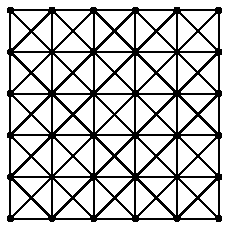
\includegraphics[width=5cm]{./images/illus136}\label{illus:136}
\]

\subsection*{Other Problems with Queens}%
\addcontentsline{toc}{section}{Other Problems with Queens and Chess-pieces}%
\markright{Problems with Queens.}%
Captain Turton\index{Turton, W.H.} called my
attention to two other problems of a somewhat analogous
character, neither of which, as far as I know, has been
published elsewhere, or solved otherwise than empirically.

The first of these is to place eight queens on a chess-board
so as to command the fewest possible squares. Thus, if queens
are placed on cells $1$ and $2$ of the second column, on cell 2 of
the sixth column, on cells $1$, $3$, and $7$ of the seventh column,
and on cells $2$ and $7$ of the eighth column, eleven cells on the
board will not be in check; the same number can be obtained
by other arrangements. Is it possible to place the eight
queens so as to leave more than eleven cells out of check?
I have never succeeded in doing so, nor in showing that it is
impossible to do it.

\PG----File: 137.png---------------------------------------------------------
The other problem is to place $m$ queens ($m$ being less than
$5$) on a chess-board so as to command as many cells as possible.
For instance, four queens can be placed in several ways on
the board so as to command $58$ cells besides those on which
the queens stand, thus leaving only $2$ cells which are not
commanded: \Eg\ this is effected if the queens are placed
on cell $5$ of the third column, cell $1$ of the fourth column, cell
$6$ of the seventh column, and cell $2$ of the eighth column; or
on cell $1$ of the first column, cell $7$ of the third column, cell
$3$ of the fifth column, and cell $5$ of the seventh column. A
similar problem is to determine the minimum number and
the position of queens which can be placed on a board of $n^2$
cells so as to occupy or command every cell. It would seem
that, even with the additional restriction that no queen shall
be able to take any other queen, there are no less than ninety-one
typical solutions in which five queens can be placed on a
chess-board so as to command every cell\footnote
{\textit{L'Intermédiaire des mathématiciens}, Paris, 1901,
vol.~\textsc{viii}, p.~88.\label{ibid:1}}%
\index{Eight Queens@\textsc{Eight Queens Problem}|)}%
\index{Queens@\textsc{Queens Problem, Eight}|)}%
\index{Queens, Problems with|)}.

\subsection*{Extension to other Chess Pieces} Analogous problems may%
\index{Chess-board, Games@\textsc{Chess-board, Games on}}%
\index{Chess-board, problems@\nobreak--- problems}
be proposed with other chess-pieces. For instance, questions
as to the maximum number of knights which can be placed
on a board of $n^2$ cells so that no knight can take any other,
and the minimum number of knights which can be placed
on it so as to occupy or command every cell have been
propounded\footnote
{\Ibidref{ibid:1}{\textit{L'Intermédiaire des mathématiciens}, Paris},
March, 1896, vol.~\textsc{iii}, p.~58; 1897, vol.~\textsc{iv},
p.~15, 254; and 1898, vol.~\textsc{v}, p.~87.}.

Similar problems have also been proposed for $k$ kings
placed on a chess-board of $n^2$ cells\footnote
{\Ibidref{ibid:1}{\textit{L'Intermédiaire des mathématiciens}, Paris},
June, 1901, p.~140.}. It has been asserted
that, if $k = 2$, the number of ways in which two kings can be
placed on a board so that they may not occupy adjacent
squares is $\frac{1}{2}(n-1)(n-2) (n^2 + 3n-2)$. Similarly, if $k=3$, the
number of ways in which three kings can be placed on a board
so that no two of them occupy adjacent squares is said to be
$\frac{1}{6}(n-1) (n-2) (n^4+ 3n^3-20n^2-30n + 132)$.
\PG----File: 138.png---------------------------------------------------------

{\ifPaper\stretchyspace\fi
\section{The Fifteen School-Girls Problem} This problem%
\index{Fifteen School@\textsc{Fifteen School-girls}|(}%
\index{Kirkman's Prob@\textsc{Kirkman's Problem}|(}%
\index{School@\textsc{School-girls, Fifteen}|(}---which
was first enunciated by Mr~T.P.~Kirkman\index{Kirkman@Kirkman, T.P.}, and is
sometimes known} as \emph{Kirkman's problem}\footnote
{It was published first in the \textit{Lady's and Gentleman's Diary} for 1850,
p.~48, and has been the subject of numerous memoirs. Among these
I may single out the papers by A.~Cayley\index{Cayley} in the \textit
{Philosophical Magazine},
July, 1850, series~3, vol.~\textsc{xxxvii}, pp.~50--53; by T.P.~Kirkman in the
\textit{Cambridge and Dublin Mathematical Journal}, 1850, vol.~\textsc{v},
p.~260; by
R.R.~Anstice\index{Anstice}, \Ibid, 1852, vol.~\textsc{vii}, pp.~279--292;
by B.~Pierce\index{Pierce on Kirkman's Problem}, \textit{Gould's
Journal}, Cambridge, U.S., 1860, vol.~\textsc{vi}, pp.~169--174; by
T.P.~Kirkman,
\textit{Philosophical Magazine}, March, 1862, series~4, vol.~\textsc{xxiii},
pp.~198--204;
by W.S.B.~Woolhouse\index{Woolhouse, Kirkman's Problem} in the \textit
{Lady's Diary} for 1862, pp.~84--88, and for
1863, pp.~79--90, and in the \textit{Educational Times Reprints}, 1867,
vol.~\textsc{viii},
pp.~76--83; by J.~Power\index{Power, Kirkman's Problem} in the \textit
{Quarterly Journal of Mathematics}, 1867,
vol.~\textsc{viii}, pp.~236--251; by A.H.~Frost\index{Frost, A.H.}, \Ibid,
1871, vol.~\textsc{xi}, pp.~26--37;
by E.~Carpmael\index{Carpmael, Kirkman's Problem} in the \textit
{Proceedings of the London Mathematical Society},
1881, vol.~\textsc{xii}, pp.~148--156; by Lucas\index{Lucas, E.} in his
\textit{Récréations}, vol.~\textsc{ii},
part~vi; by A.C.~Dixon\index{Dixon, A.C.} in the \textit{Messenger of
Mathematics}, Cambridge,
October, 1893, vol.~\textsc{xxiii}, pp.~88--89; and by W.~Burnside\index
{Burnside, Kirkman's Problem}, \Ibid, 1894,
vol.~\textsc{xxiii}, pp.~137--143. It has also, since the issue of my third
edition,
been discussed by W.~Ahrens\index{Ahrens} in his \textit{Mathematische
Unterhaltungen und
Spiele}, Leipzig, 1901, chapter~xiv.}---consists in arranging
fifteen things in different sets of triplets. It is usually
presented in the form that a school-mistress was in the habit
of taking her girls for a daily walk. The girls were fifteen
in number, and were arranged in five rows of three each so
that each girl might have two companions. The problem is
to dispose them so that for seven consecutive days no girl will
walk with any of her school-fellows more than once. More
generally we may require to arrange $3m$ girls in triplets to
walk out for $\frac{1}{2}(3m-1)$ days, so that no girl will walk with
any of her school-fellows more than once.

The theory of the formation of all such possible triplets in
the case of fifteen girls is not difficult, but the extension to
$3m$ girls is, as yet, unsolved\Editorial
{In 1971 Ray-Chaudhuri and Wilson proved that Kirkman triple systems of
order $\nu$ exist if and only if $\nu\equiv3\pmod 6$}.
I proceed to describe three
methods of solution: these methods are analytical, but I may
add that the problem can be also attacked by geometrical
methods.

\PG----File: 139.png------------------------------------------------------
\subsection*{Frost's Method}
The first of these solutions is due to Mr~Frost\index{Frost, A.H.|(}.
A full exposition of it would occupy a good deal of
space, but I hope that the following sketch will make the
process intelligible.

Denote one of the girls by $k$. Her companions on each
day are different: suppose that on Sunday they are $a_1$ and $a_2$,
on Monday $b_1$ and $b_2$, and so on, and finally on Saturday $g_1$
and $g_2$. Hence for each day we have one triplet, and we have
to find four others, but in each of the latter no two like letters
can occur together, that is, the three letters in any of them
must be all different.

Let $a$ stand for $a_1$, or $a_2$, $b$ for $b_1$ or $b_2$, and so on. The
suffixes $1$ and $2$ are called complementary. Then, since the
three letters in each of the triplets we are trying to find must
be different, we must make some arrangement such as putting
$a$ with $bc$, $de$, and $fg$; and, if so, $b$ may be associated with $df$
and $eg$; and $c$ with $dg$ and $ef$. Thus there are seven possible
triads, such as $abc$, $ade$, $afg$, $bdf$, $beg$, $cdg$, and $cef$. Moreover
each of these may stand for any one of four triplets: for
instance, the triad $bdf$ may stand for any of the triplets
$b_1 d_1 f_1$, $b_1 d_2 f_2$, $b_2 d_1 f_2$, $b_2 d_2 f_1$.

The four triads which do not involve $a$ must be placed in the
Sunday column, the four which do not involve $b$ in the Monday
column, and so on. Thus each triad will occur four times.

It only remains to insert the proper suffixes. This is done
as follows. Take one triad, such as $bdf$, and insert a different
set of suffixes each time that it occurs; for instance, the four
sets given above. Next, the other like letters ($b$, $d$, or $f$ as the
case may be) in these four columns must have the complementary
suffixes attached.

After this is done, the next triplet in the Sunday column
will be $b_2 eg$. The triad $beg$ occurs in four columns and includes
four possible triplets, such as
$b_2 e_1 g_1$, $b_2 e_2 g_2$, $b_1 e_1 g_2$, $b_1 e_2 g_1$. Insert
these, and then give the complementary suffixes to the other
like letters in these four columns.

In this way the arrangement is constructed gradually, by
\PG----File: 140.png------------------------------------------------------
taking one triad at a time, inserting the proper suffixes to the
four triplets included in it, and then the complementary
suffixes in the other like letter in the same columns.

One final arrangement, thus obtained, is as follows:{\ifPaper\smaller\fi
\[
\begin{array}{|c|c|c|c|c|c|c|}
\hline
\text{\smaller Sunday}\DParraykludge
 & \text{\smaller Monday} & \text{\smaller Tuesday}
 & \text{\smaller Wednesday} & \text{\smaller Thursday}
 & \text{\smaller Friday} & \text{\smaller Saturday}\\[3pt]
\hline
  k a_1 a_2 \DParraykludge
& k b_1 b_2 & k c_1 c_2 & k d_1 d_2
& k e_1 e_2 & k f_1 f_2 & k g_1 g_2
\\
  b_1 d_1 f_1 & a_1 d_2 e_2 & a_1 d_1 e_1 & a_2 b_2 c_2
& a_2 b_1 c_1 & a_1 b_2 c_1 & a_1 b_1 c_2
\\
  b_2 e_1 g_1 & a_2 f_2 g_2 & a_2 f_1 g_1 & a_1 f_2 g_1
& a_1 f_1 g_2 & a_2 d_2 e_1 & a_2 d_1 e_2
\\
  c_1 d_2 g_2 & c_1 d_1 g_1 & b_1 d_2 f_2 & b_1 e_1 g_2
& b_2 d_1 f_2 & b_1 e_2 g_1 & b_2 d_2 f_1
\\
  c_2 e_2 f_2 & c_2 e_1 f_1 & b_2 e_2 g_2 & c_1 e_2 f_1
& c_2 d_2 g_1 & c_2 d_1 g_2 & c_1 e_1 f_2
\\[6pt]
\hline
\end{array}
\]
}We might obtain other solutions by selecting other seven
triads or by choosing other arrangements of the suffixes in
each triad (or by merely interchanging letters and suffixes in
the above order). By these means Mr~Power\index{Power, Kirkman's Problem}
showed that
there are no less than $15567,552000$ different solutions; but,
since the total number of ways in which the school can walk
out for a week in triplets is $(455)^7$, the probability that any
chance way satisfies Kirkman's condition is very small.

Frost's method is applicable to the case of $2^{2n}-1$ girls
walking out for $2^{2n-1}-1$ days in triplets. The detailed
solution for $63$ girls walking out for $31$ days, which corresponds
to $n = 3$, have been given\index{Frost, A.H.|)}.

\subsection*{Anstice's Method} Another method of attacking\index{Anstice|(}
the problem is due to Mr Anstice; it is illustrated by the following
elegant solution, by which from the order on Sunday we can
obtain the order on the following six days by a cyclical permutation.
Let the girls be denoted respectively by the letters
$k$, $a_1$, $a_2$, $a_3$, $a_4$, $a_5$, $a_6$, $a_7$,
$b_1$, $b_2$, $b_3$, $b_4$, $b_5$, $b_6$, $b_7$; and suppose
the order on Sunday to be
\[
  k a_1 b_1,\; a_2 a_3 a_5,\; a_4 b_3 b_6,\; a_6 b_2 b_7,\; a_7 b_4 b_5\,.
\]
Then, if the suffixes are permuted cyclically, we obtain six
other arrangements which satisfy the conditions of the problem:
the reason being that in the above arrangement the difference
\PG----File: 141.png----------------------------------------------------
of the suffixes of every pair of like letters---such as either the
``$a$''s or the ``$b$''s---in a triplet is different for each triplet, as
also is the difference of the suffixes of every pair of unlike
letters which are in a triplet.

Two other arrangements for Sunday, from which those for
the remaining days are obtainable by cyclical permutations
can be formed. These are $ka_1b_1$, $a_2a_3a_5$, $a_4b_5b_7$, $a_6b_3b_4$,
$a_7b_2b_6$;
and $ka_1b_1$, $a_2a_3a_5$, $a_4b_2b_6$, $a_6b_5b_7$, $a_7b_3b_4$.

Anstice's method is applicable to the case of $2p+1$ girls
walking out for $p$ days in triplets so that no pair may walk
together more than once, provided $p$ is a prime of the form
$12m+7$. In such a case he showed how to construct a fundamental
arrangement for one day from which the arrangements
for the remaining $p-1$ days can be obtained by cyclical
permutations of suffixes. The number of such fundamental
arrangements is $3 (2m+1)(3m+1)$.

The problem of $15$ girls corresponds to $m = 0$, and the
three fundamental Anstician arrangements are given above.
If $m=1$ we have the problem of $39$ girls. One Anstician
arrangement in this case is as follows: $ka_1b_1$, $a_2a_8a_{12}$,
$a_5a_7a_{10}$,
$a_6a_{17}a_{18}$, $a_3b_{10}b_{15}$, $a_4b_3b_5$, $a_9b_{18}b_{19}$,
$a_{11}b_8b_{14}$, $a_{13}b_9b_{17}$, $a_{14}b_{12}b_{16}$,
$a_{15}b_4b_7$, $a_{16}b_2b_{11}$, $a_{19}b_6b_{13}$. If $m=2$ we have the
problem of $63$
girls, of which Frost has given one solution; and so on.\index{Anstice|)}

\subsection*{Gill's Method} Another method of attacking the problem
has been suggested to me by Mr~T.H.~Gill\index{Gill, Kirkman's Problem|(}.
Representing
the girls by $a_1, a_2, a_3, \dotsc, a_{3m}$ he (i)~forms one triplet of the
type $a_1a_{m+1}a_{2m+1}$, from which, by cyclical permutation of the
suffixes $1, 2, \dotsc, 3m$ he obtains $m$ triplets which constitute an
arrangement for one day, and (ii)~forms $\frac{1}{2}(m-1)$ other triplets
such that the three differences of the suffixes are different,
from which, by cyclical permutations of the suffixes, the
arrangements for the remaining $\frac{3}{2}(m-1)$ other days can be
obtained. Thus in the case of $15$ girls, the triplet $a_1a_6a_{11}$
gives, by cyclical permutations of the suffixes, an arrangement
for the first day and two triplets such as $a_1a_2a_5$, $a_1a_3a_9$ enable
us to form $30$ triplets from which an arrangement for the
\PG----File: 142.png----------------------------------------------------
other six days can be found. Here is a solution thus
determined.
\[\text{\relsize{-2}
\begin{tabular}{l r@.r@.r r@.r@.r r@.r@.r r@.r@.r r@.r@.r}
  First Day:  &  1& 6&11;& 2& 7&12;& 3& 8&13;& 4& 9&14;& 5&10&15\,.\\
  Second Day: &  1& 2& 5;& 3& 4& 7;& 8& 9&12;&10&11&14;&13&15& 6\,.\\
  Third Day:  &  2& 3& 6;& 4& 5& 8;& 9&10&13;&11&12&15;&14& 1& 7\,.\\
  Fourth Day: &  5& 6& 9;& 7& 8&11;&12&13& 1;&14&15& 3;& 2& 4&10\,.\\
  Fifth Day:  &  7& 9&15;& 8&10& 1;& 3& 5&11;& 4& 6&12;&13&14& 2\,.\\
  Sixth Day:  &  9&11& 2;&10&12& 3;& 5& 7&13;& 6& 8&14;&15& 1& 4\,.\\
  Seventh Day:& 11&13& 4;&12&14& 5;&15& 2& 8;& 1& 3& 9;& 6& 7&10\,.\\
\end{tabular}}\]
But, although this method gives triplets with which the
problem can be solved, the final arrangement is empirical\index
{Gill, Kirkman's Problem|)}.

A solution of the problem of $21$ girls for $10$ days can be
got by the same method: $a_1a_8a_{15}$ giving $7$ triplets which
constitute an arrangement for one day; and $a_1a_2a_6$, $a_1a_3a_{11}$,
$a_1a_4a_{10}$ giving $63$ triplets from which an arrangement for the
other nine days can be formed. Here is the solution thus
determined.
\[\hss\ifPaper\def\tabcolsep{4pt}\fi
\text{\relsize{-2}\begin{tabular}
{l r@.r@.r r@.r@.r r@.r@.r r@.r@.r r@.r@.r r@.r@.r r@.r@.r}
First Day:& 1&8&15;& 2&9&16;& 3&10&17;& 4&11&18;& 5&12&19;&
 6&13&20;& 7&14&21\,.\\
Second Day:& 1&2&6;& 4&5&9;& 7&8&12;& 10&11&15;& 13&14&18;&
 16&17&21;& 19&20&3\,.\\
Third Day:& 7&10&16;& 8&11&17;& 12&15&21;& 18&19&2;& 20&1&9;&
 3&5&13;& 4&6&14\,.\\
Fourth Day:& 13&16&1;& 14&17&2;& 18&21&6;& 3&4&8;& 5&7&15;&
 9&11&19;& 10&12&20\,.\\
Fifth Day:& 4&7&13;& 5&8&14;& 9&12&18;& 15&16&20;& 17&19&6;&
 21&2&10;& 1&3&11\,.\\
Sixth Day;& 1&4&10;& 2&5&11;& 6&9&15;& 12&13&17;& 14&16&3;&
 18&20&7;& 19&21&8\,.\\
Seventh Day:& 2&3&7;& 5&6&10;& 8&9&13;& 11&12&16;& 14&15&19;&
 17&18&1;& 20&21&4\,.\\
Eighth Day:& 10&13&19;& 11&14&20;& 15&18&3;& 21&1&5;& 2&4&12;&
 6&8&16;& 7&9&17\,.\\
Ninth Day:& 16&19&4;& 17&20&5;& 21&3&9;& 6&7&11;& 8&10&18;&
 12&14&1;& 13&15&2\,.\\
Tenth Day:& 19&1&7;& 20&2&8;& 3&6&12;& 9&10&14;& 11&13&21;&
 15&17&4;& 16&18&5\,.\\
\end{tabular}}\hss\]

I should be interested if any of my readers could give me
a similar solution of the analogous arrangement of $33$ girls for
$16$ days formed from typical triplet suffixes like $1$, $12$, $23$; $1$,
$2$, $10$; $1$, $3$, $16$; $1$, $4$, $18$; $1$, $5$, $11$; $1$, $6$, $13$;
or from other
sets of triplets formed in a similar way so that (except in the
first triplet) the differences of the suffixes are all different.

{\ifPaper\stretchyspace\fi
\subsection*{Walecki's Theorem} Lastly, Walecki\index
{Walecki}---quoted by Lucas\index{Lucas, E.}---has
shown that}, if a solution for the case of $n$ girls walking
\PG----File: 143.png----------------------------------------------------
out in triplets for $\frac{1}{2}(n-1)$ days is known, then a solution for
$3n$ girls walking out for $\frac{1}{2}(3n-1)$ days can be deduced.

For if an arrangement of the $n$ girls, $a_1, a_2, \dotsc, a_n$ for
$\frac{1}{2}(n-1)$ days is known; and also one of the $n$ girls,
$b_1, b_2,\dotsc, b_n$;
and also one of the $n$ girls $c_1, c_2, \dotsc, c_n$; then an arrangement
of these $3n$ girls for $\frac{1}{2}(n-1)$ days is known. A set of $n$
triplets for another day will be given by $a_mb_{m+k}c_{m + 2k}$ where $m$
is put equal to $1, 2, \dotsc, n$ successively. Here $k$ may have any
of the $n$ values, $0, 1, 2, \dotsc, (n-1)$; but, wherever a suffix is
greater than $n$, it is to be divided by $n$ and only the remainder
retained. Hence altogether we have an arrangement for
${n + \frac{1}{2} (n-1)}$ days, \IE\ for $\frac{1}{2}(3n-1)$ days.

The arrangement of $3$ girls for one day is obvious. Hence,
by Walecki's\index{Walecki} theorem, we can deduce at once an arrangement
of $3^m$ girls for $\frac{1}{2}(3^m-1)$ days. And, generally, as I have
given solutions of the problem in the case of $3n$ girls when
$n= 1$, $3$, $5$, $7$, $9$, $13$, $15$, it follows that for the same values
of $n$,
we can solve the analogous arrangements of $3^m \times n$ girls.

To the original theorem J.J.~Sylvester\index{Sylvester}\footnote
{\textit{Philosophical Magazine}, July, 1850, series~3, vol.~\textsc{xxxvii},
p.~52;
a solution by Sylvester is given in the \textit{Philosophical Magazine}, May,
1861, series~4, vol.~\textsc{xxi}, p.~371.} added the
corollary that the school of $15$ girls could walk out in
triplets on $13\times 7$ days until every possible triplet had walked
abreast once.

The generalized problem of finding the greatest number of
ways in which $x$ girls walking in rows of $a$ abreast can be
arranged so that every possible combination of $b$ of them may
walk abreast once and only once has been solved for various
cases. Suppose that this greatest number of ways is $y$. It
is obvious that, if all the $x$ girls are to walk out each day in
rows of $a$ abreast, then $x$ must be an exact multiple of $a$ and
the number of rows formed each day is $x/a$. If such an
arrangement can be made for $z$ days, then we have a solution
of the problem to arrange $x$ girls to walk out in rows of $a$
abreast for $z$ days so that they all go out each day and so that
\PG----File: 144.png----------------------------------------------------
every possible combination of $b$ girls may walk together once,
and only once. In the corresponding generalization of Kirkman's
problem no companionship of girls which has occurred
once may occur again, but it does not follow necessarily that
every possible companionship must occur once.

An example where the solution is obvious is if $x=2n$, $a=2$,
$b=2$, in which case $y=n(2n-1)$, $z=2n-1$.

If we take the case $x=15$, $a=3$, $b=2$, we find $y=35$; and
it happens that these $35$ rows can be divided into $7$ sets,
each of which contains all the symbols; hence $z=7$. More
generally, if $x=5 \times 3^m$, $a=3$, $b=2$, we find $y=\frac{3}{2}(x-1)/x$,
$z=\frac{1}{2}(x-1)$. It will be noticed that in the solutions of the
original fifteen school-girls problem and of Walecki's extension
of it given above every possible pair of girls walk together
once; hence we might infer that in these cases we could
determine $z$ as well as $y$.

The results of the last paragraph were given by Kirkman\index
{Kirkman@Kirkman, T.P.}\footnote
{\textit{Cambridge and Dublin Mathematical Journal}, 1850, vol.~\textsc{v},
pp.~255--262.\label{ibid:2}}
in 1850. In the same memoir he also proved that, if $p$ is a
prime, and if $x=p^m$, $a=p$, $b=2$, then $y=(p^m-1)/(p-1)$;
if $x=(p^2+p+1)(p+1)$ where $p^2+p+1$ has no divisor less
than $p+1$, $a=p+1$, $b=2$, then $y=x(x-1)/p(p+1)$; if
$x=p^3+p+1$, $a=p+1$, $b=2$, then $y=x$; and Sylvester's\index{Sylvester}
result that if $x=15$, $a=3$, $b=3$, $y=455$, $z=91$. Three years
later Kirkman\footnote
{\Ibidref{ibid:2}{\textit{Cambridge and Dublin Mathematical Journal}},
1853, vol.~\textsc{viii}, pp.~38--42.}
solved the problem when $x=2^n$, $a=4$,
$b=3$. Lastly, in 1893, Sylvester\footnote
{\textit{Messenger of Mathematics}, February, 1893, vol.~\textsc{xxii},
pp.~159--160.} published the solution when
$x=9$, $a=3$, $b=3$, in which case $y=84$, $z=28$; and stated that
a similar method was applicable when $x=3^m$, $a=3$, $b=3$: thus
$9$ girls can be arranged to walk out $28$ times (say $4$ times a
day for a week) so that in any day the same pair never are
together more than once and so that at the end of the week
each girl has been associated with every possible pair of her
schoolfellows.

\PG----File: 145.png----------------------------------------------------
In 1867 Mr~S.~Bills\index{Bills on Kirkman's Problem}\footnote
{\textit{Educational Times Reprints}, London, 1867, vol.~\textsc{viii},
pp.~32--33.\label{ibid:3}} showed that if $x=7$, $a=3$, $b=2$,
then $y=7$: if $x=15$, $a=3$, $b=2$, then $y=35$: if $x=31$, $a=3$,
$b=2$, then $y=155$: and the method by which these results
are proved will give the value of $y$, if $x=2^n-1$, $a=3$, $b=2$.
Shortly afterwards Mr~W.~Lea\index{Lea on Kirkman's Problem}\footnote
{\Ibidref{ibid:3}{\textit{Educational Times Reprints}, London},
1868, vol.~\textsc{ix}, pp.~35--36; and 1874, vol.~\textsc{xxii},
pp.~74--76; see also the volume for 1869, vol.~\textsc{xi}, p.~97.} showed
that if $x=11$,
$a=5$, $b=4$, then $y=66$; also that if $x=16$, $a=4$, $b=3$, then
$y=140$; the latter result is a particular case of Kirkman's
theorems. It will be noticed that these writers did not confine
their discussion to cases where $x$ is an exact multiple of $a$\index
{Fifteen School@\textsc{Fifteen School-girls}|)}%
\index{Kirkman's Prob@\textsc{Kirkman's Problem}|)}%
\index{School@\textsc{School-girls, Fifteen}|)}.

\section[Problems connected with a pack of cards]%
{Problems connected with a Pack of Cards} I mentioned
in \hyperlink{chapter:1:cards}{chapter~\textsc{i}} that an ordinary pack
of playing cards\index{Cards, Problems with|(}
could be used to illustrate many tricks depending on simple
properties of numbers. Most of these involve the relative
position of the cards. The principle of solution generally
consists in re-arranging the pack in a particular manner so as
to bring the card into some definite position. Any such rearrangement
is a species of shuffling.

I shall treat in succession of problems connected with\index
{Shuffling@\textsc{Shuffling Cards}|(}
\emph{shuffling a pack}, \emph{arrangements by rows and columns}, the
\emph{determination of a pair out of $\frac{1}{2}n(n+1)$ pairs},
\emph{Gergonne's pile
problem}, and the game known as \emph{the mouse trap}.

\section*{Shuffling a Pack}%
\addcontentsline{toc}{subsection}{Monge on shuffling a pack of cards}
Any system of \emph{shuffling a pack}\index{Monge on Shuffling Cards|(} of
cards, if carried out consistently, leads to an arrangement
which can be calculated; but tricks that depend on it generally
require considerable technical skill.

Suppose for instance that a pack of $n$ cards is shuffled, as
is not unusual, by placing the second card on the first, the
third below these, the fourth above them, and so on. The
theory of this system of shuffling is due to Monge\footnote
{Monge's investigations are printed in the \textit{Mémoires de l'Académie
des Sciences}, Paris, 1773, pp.~390--412. Among those who have studied
the subject afresh I may in particular mention V.~Bouniakowski\index
{Bouniakowski, V., on shuffling}, \textit{Bulletin
physico-mathématique de St Pétersbourg}, 1857, vol.~\textsc{xv},
pp.~202--205,
summarised in the \textit{Nouvelles annales de mathématiques}, 1858,
pp.~66--67; T.~de St~Laurent\index{DeSaint@De St Laurent}\index
{StL@St Laurent on cards}, \textit{Mémoires de l'Académie de Gard}, 1865;
L.~Tanner\index{Tanner on Shuffling Cards}, \textit{Educational Times
Reprints}, 1880, vol.~\textsc{xxxiii}, pp.~73--75;
and M.J.~Bourget\index{Bourget, M.J., on shuffling}, \textit{Liouville's
Journal}, 1882, pp.~413--434. The solutions
given by Prof.\ Tanner are simple and concise.}. The
\PG----File: 146.png----------------------------------------------------
following are some of the results and are not difficult to prove
directly.

If the pack contains $6p+4$ cards, the $(2p + 2)$th card will
occupy the same position in the shuffled pack. For instance,
if a complete pack of $52$ cards is shuffled as described above,
the $18$th card will remain the $18$th card.

Again, if a pack of  $10p + 2$ cards is shuffled in this way,
the $(2p + 1)$th and the $(6p \times 2)$th cards will interchange places.
For instance, if an écarté pack of $32$ cards is shuffled as described
above, the $7$th and the $20$th cards will change places.

More generally, one shuffle of a pack of $2p$ cards will
move the card which was in the $x_0$th place to the $x_1$th place,
where $x_1=\frac{1}{2}(2p+x_0+1)$ if $x_0$ is odd, and
$x_1=\frac{1}{2}(2p-x_0 + 2)$
if $x_0$ is even, from which the above results can be deduced.
By repeated applications of the above formulae we can
show that the effect of $m$ such shuffles is to move the card
which was initially in the $x_0$th place to the $x_m$th place where
$2^{m+1}x_m=(4p+1)(2^{m-1} \pm 2^{m-2} \pm \dotsb \pm 2 \pm 1)
\pm 2x_0 + 2^m \pm 1$, the
sign $\pm$ representing an ambiguity of sign.

Again, in any pack of $n$ cards after a certain number of
shufflings, not greater than $n$, the cards will return to their
primitive order. This will always be the case as soon as the
original top card occupies that position again. To determine
the number of shuffles required for a pack of $2p$ cards, it is
sufficient to put $x_m=x_0$ and find the smallest value of $m$
which satisfies the resulting equation for all values of $x_0$
from $1$ to $2p$. It follows that, if $m$ is the least number
which makes $4^m-1$ divisible by $4p+1$, then $m$ shuffles will be
required if either $2^m+1$ or $2^m-1$ is divisible by $4p+1$, otherwise
$2m$ shuffles will be required. The number for a pack of
\PG----File: 147.png----------------------------------------------------
$2p+1$ cards is the same as that for a pack of $2p$ cards. With
an écarté pack of $32$ cards, six shuffles are sufficient; with
a pack of $2^n$ cards, $n+1$ shuffles are sufficient; with a full
pack of $52$ cards, twelve shuffles are sufficient; with a pack
of $13$ cards ten shuffles are sufficient; while with a pack of
$50$ cards fifty shuffles are required; and so on\index
{Monge on Shuffling Cards|)}.

Mr W.H.H.~Hudson\index{Hudson, W.H.H., on cards}\footnote
{\textit{Educational Times Reprints}, London, 1865, vol.~\textsc{ii}, p.~105.}
has also shown that, whatever is
the law of shuffling, yet if it is repeated again and again on
a pack of $n$ cards, the cards will ultimately fall into their
initial positions after a number of shufflings not greater than
the greatest possible \textsc{l.c.m.} of all numbers whose sum is $n$.

For suppose that any particular position is occupied after
the $1$st, $2$nd, $\dots$, $p$th shuffles by the cards
$A_1, A_2, \dotsc, A_p$ respectively,
and that initially the position is occupied by the
card $A_0$. Suppose further that after the $p$th shuffle $A_0$ returns
to its initial position, therefore $A_0=A_p$. Then at the second
shuffling $A_2$ succeeds $A_1$ by the same law by which $A_1$ succeeded
$A_0$ at the first; hence it follows that previous to the
second shuffling $A_2$ must have been in the place occupied by
$A_1$ previous to the first. Thus the cards which after the
successive shuffles take the place initially occupied by $A_1$ are
$A_2, A_3, \dotsc, A_p, A_1$; that is, after the $p$th shuffle $A_1$
has returned
to the place initially occupied by it: and so for all the
other cards $A_2, A_3, \dotsc, A_{p-1}$.

Hence the cards $A_1, A_2, \dotsc, A_p$ form a cycle of $p$ cards, one
or other of which is always in one or other of $p$ positions in the
pack, and which go through all their changes in $p$ shufflings.
Let the number $n$ of the pack be divided into $p, q, r, \ldots$ such
cycles, whose sum is $n$; then the \textsc{l.c.m.} of $p, q, r, \ldots$
is the
utmost number of shufflings necessary before all the cards will
be brought back to their original places.

In the case of a pack of $52$ cards, the greatest \textsc{l.c.m.} of
numbers whose sum is $52$ will be found by trial to be
$180180$\index{Shuffling@\textsc{Shuffling Cards}|)}.

\PG----File: 148.png----------------------------------------------------
\section*{Arrangements by Rows and Columns}%
\addcontentsline{toc}{subsection}{Arrangement by rows and columns}
A not uncommon
trick, which rests on a species of shuffling, depends on the
obvious fact that if $n^2$ cards are arranged in the form of a
square of $n$ rows, each containing $n$ cards, then any card
will be defined if the row and the column in which it lies are
mentioned.

This information is generally elicited by first asking in
which row the selected card lies, and noting the extreme left-hand
card of that row. The cards in each column are then
taken up, face upwards, one at a time beginning with the
lowest card of each column and taking the columns in their
order from right to left--each card taken up being placed on
the top of those previously taken up. The cards are then
dealt out again in rows, from left to right, beginning with the
top left-hand corner, and a question is put as to which row
contains the card. The selected card will be that card in the
row mentioned which is in the same vertical column as the
card which was originally noted.

The above is the form in which the trick is usually
presented, but it is greatly improved by allowing the pack to
be cut as often as is liked before the cards are re-dealt, and
then giving one cut at the end so as to make the top card in
the pack one of those originally in the top row.

The explanation is obvious. For, if $16$ cards are taken,
\begin{figure*}[!hbt]
\def\SqHt{3em}
\def\SqWd{2em}
\unitlength=1em
\centering
\hspace*{\fill}
\begin{minipage}{0.4\textwidth}
\centering
\begin{picture}(11,15)
\Cell(0,12;1)\Cell(3,12;2)\Cell(6,12;3)\Cell(9,12;4)
\Cell(0,8;5)\Cell(3,8;6)\Cell(6,8;7)\Cell(9,8;8)
\Cell(0,4;9)\Cell(3,4;10)\Cell(6,4;11)\Cell(9,4;12)
\Cell(0,0;13)\Cell(3,0;14)\Cell(6,0;15)\Cell(9,0;16)
\end{picture}
\legend{Figure \Uproman{1}}
\end{minipage}
\hfill
\begin{minipage}{0.4\textwidth}
\centering
\begin{picture}(11,15)
\Cell(0,12;1)\Cell(3,12;5)\Cell(6,12;9)\Cell(9,12;13)
\Cell(0,8;2)\Cell(3,8;6)\Cell(6,8;10)\Cell(9,8;14)
\Cell(0,4;3)\Cell(3,4;7)\Cell(6,4;11)\Cell(9,4;15)
\Cell(0,0;4)\Cell(3,0;8)\Cell(6,0;12)\Cell(9,0;16)
\end{picture}
\legend{Figure \Uproman{2}}
\end{minipage}
\hspace*{\fill}
\end{figure*}
the first and second arrangements may be represented by
\PG----File: 149.png----------------------------------------------------
figures~i and ii. For example, if we are told that in figure~i
the card is in the third row, it must be either $9$, $10$, $11$, or $12$:
hence, if we know in which row of figure~ii it lies, it is determined.
If we allow the pack to be cut between the deals,
we must secure somehow that the top card is either $1$, $2$, $3$,
or $4$, since that will leave the cards in each row of figure~ii
unaltered though the positions of the rows will be changed.

\section*{Determination of a selected pair of cards out of
$\protect\frac{1}{2}n(n+1)$ given pairs\protect\footnote
{Bachet\index{Bachet@Bachet's \textit{Problèmes}}, problem~\textsc{xvii},
avertissement, p.~146 \etseq}}%
\addcontentsline{toc}{subsection}{Determination of one out of
\texorpdfstring{$\protect\frac12n(n+1)$}{\textonehalf n(n+1)} given couples}
Another common trick is to throw
twenty cards on to a table in ten couples, and ask someone
to select one couple\index{Pairs of Cards Trick|(}.
The cards are then taken up, and dealt
out in a certain manner into four rows each containing five
cards. If the rows which contain the given cards are indicated,
the cards selected are known at once.

This depends on the fact that the number of homogeneous
products of two dimensions which can be formed out of four
things is $10$. Hence the homogeneous products of two dimensions
formed out of four things can be used to define ten things.

Suppose that ten pairs of cards are placed on a table and
someone selects one couple. Take up the cards in their
\begin{figure*}[!hbt]
\centering
\def\SqHt{3em}
\def\SqWd{2em}
\unitlength=1em
\begin{picture}(14,15)
\Cell(0,12;1)\Cell(3,12;2)\Cell(6,12;3)\Cell(9,12;5)\Cell(12,12;7)
\Cell(0,8;4)\Cell(3,8;9)\Cell(6,8;10)\Cell(9,8;11)\Cell(12,8;13)
\Cell(0,4;6)\Cell(3,4;12)\Cell(6,4;15)\Cell(9,4;16)\Cell(12,4;17)
\Cell(0,0;8)\Cell(3,0;14)\Cell(6,0;18)\Cell(9,0;19)\Cell(12,0;20)
\end{picture}
\end{figure*}
couples. Then the first two cards form the first couple, the
next two the second couple, and so on. Deal them out in
four rows each containing five cards according to the scheme
shown in the diagram. % [**Note: originally "above"]

\PG----File: 150.png----------------------------------------------------
The first couple ($1$ and $2$) are in the first row. Of the next
couple ($3$ and $4$), put one in the first row and one in the
second. Of the next couple ($5$ and $6$), put one in the first
row and one in the third, and so on, as indicated in the
diagram. After filling up the first row proceed similarly with
the second row, and so on.

Enquire in which rows the two selected cards appear. If
only one line, the $m$th, is mentioned as containing the cards
then the required pair of cards are the $m$th and $(m+1)$th
cards in that line. These occupy the clue squares of that
line. Next, if two lines are mentioned, then proceed as
follows. Let the two lines be the $p$th and the $q$th and suppose
$q>p$. Then that one of the required cards which is in the
$q$th line will be the $(q-p)$th card which is below the first
of the clue squares in the $p$th line. The other of the required
cards is in the $p$th line and is the $(q-p)$th card to the right of
the second of the clue squares.

Bachet's rule, in the form in which I have given it, is
applicable to a pack of $n(n+1)$ cards divided into couples,
and dealt in $n$ rows each containing $n+1$ cards; for there are
$\frac{1}{2}n(n+1)$ such couples, also there are $\frac{1}{2}n(n+1)$
homogeneous
products of two dimensions which can be formed out of $n$
things. Bachet gave the diagrams for the cases of $20$, $30$, and
$42$ cards: these the reader will have no difficulty in constructing
for himself, and I have enunciated the rule for $20$ cards in
a form which covers all the cases.

I have seen the same trick performed by means of a sentence
and not by numbers. If we take the case of ten couples, then
after collecting the pairs the cards must be dealt in four rows
each containing five cards, in the order indicated by the
sentence \emph{Matas dedit nomen Cocis}. This sentence must be
imagined as written on the table, each word forming one line,
The first card is dealt on the $M$. The next card (which is the
pair of the first) is placed on the second $m$ in the sentence,
that is, third in the third row. The third card is placed on
the $a$. The fourth card (which is the pair of the third) is
\PG----File: 151.png---------------------------------------------------------
placed on the second $a$, that is, fourth in the first row. Each
of the next two cards is placed on a $t$, and so on. Enquire
in which rows the two selected cards appear. If two rows
are mentioned, the two cards are on the letters common to
the words that make these rows. If only one row is mentioned,
the cards are on the two letters common to that row.

The reason is obvious: let us denote each of the first
pair by an $a$, and similarly each of any of the other pairs
by an $e$, $i$, $o$, $c$, $d$, $m$, $n$, $s$, or $t$ respectively.
Now the sentence
\emph{Matas dedit nomen Cocis} contains four words each of five
letters; ten letters are used, and each letter is repeated only
twice. Hence, if two of the words are mentioned, they will
have one letter in common, or, if one word is mentioned, it will
have two like letters.

To perform the same trick with any other number of cards
we should require a different sentence.

The number of homogeneous products of three dimensions
which can be formed out of four things is $20$, and of these the
number consisting of products in which three things are alike
and those in which three things are different is $8$. This leads
to a trick with $8$ trios of things, which is similar to that last
given--the cards being arranged in the order indicated by the
sentence \emph{Lanata levete livini novoto}.

I believe that these arrangements by sentences are
known, but I am not aware who invented them\index{Pairs of Cards Trick|)}.

\section*{Gergonne's Pile Problem}%
\addcontentsline{toc}{subsection}{Gergonne's Pile Problem}
Before discussing Gergonne's%
\index{Gergonne@\textsc{Gergonne's Problem}|(}%
\index{Pile@\textsc{Pile Problems}|(}
theorem I will describe the familiar three pile problem, the
theory of which is included in his results.

\subsection*{The Three Pile Problem\protect\footnote
{The trick is mentioned by Bachet\index{Bachet@Bachet's \textit{Problèmes}},
problem \textsc{xviii}, p.~143, but his
analysis of it is insufficient.}} This trick\index
{Three-pile@\textsc{Three-pile Problem}|(} is usually performed
as follows. Take $27$ cards and deal them into three piles,
face upwards. By ``dealing'' is to be understood that the top
card is placed as the bottom card of the first pile, the second
card in the pack as the bottom card of the second pile, the
\PG----File: 152.png----------------------------------------------------
third card as the bottom card of the third pile, the fourth card
on the top of the first one, and so on: moreover I assume
that throughout the problem the cards are held in the hand
face upwards. The result can be modified to cover any other
way of dealing.

Request a spectator to note a card, and remember in which
pile it is. After finishing the deal, ask in which pile the card
is. Take up the three piles, placing that pile between the
other two. Deal again as before, and repeat the question as
to which pile contains the given card. Take up the three
packs again, placing the pile which now contains the selected
card between the other two. Deal again as before, but in
dealing note the middle card of each pile. Ask again for the
third time in which pile the card lies, and you will know that
the card was the one which you noted as being the middle
card of that pile. The trick can be finished then in any way
that you like. The usual method\label{page:152}---but a very clumsy one---is
to take up the three piles once more, placing the named
pile between the other two as before, when the selected card
will be the middle one in the pack, that is, if $27$ cards are
used it will be the fourteenth.

The trick is often performed with $15$ cards or with $21$ cards,
in either of which cases the same rule holds.

\subsection*{Gergonne's Generalization} The general theory for a pack
of $m^m$ cards was given by M.~Gergonne\footnote
{Gergonne's \textit{Annales de Mathématiques}, Nismes, 1813--4,
vol.~\textsc{iv}, pp.~276--283.}. Suppose the pack
is arranged in $m$ piles, each containing $m^{m-1}$ cards, and that,
after the first deal, the pile indicated as containing the selected
card is taken up $a$th; after the second deal, is taken up $b$th;
and so on, and finally after the $m$th deal, the pile containing
the card is taken up $k$th. Then when the cards are collected
after the $m$th deal the selected card will be $n$th from the top
where
\[
\begin{array}{ll}
\text{if $m$ is even,}& n=km^{m-1}-jm^{m-2} + \dotsb + bm - a + 1\,,\\
\text{if $m$ is odd,}& n=km^{m-1}-jm^{m-2} + \dotsb - bm + a\,.
\end{array}
\]

\PG----File: 153.png---------------------------------------------------------
For example, if a pack of $256$ cards (\IE\ $m = 4$) was given,
and anyone selected a card out of it, the card could be determined
by making four successive deals into four piles of
$64$ cards each, and after each deal asking in which pile the
selected card lay. The reason is that after the first deal you
know it is one of sixty-four cards. In the next deal these
sixty-four cards are distributed equally over the four piles,
and therefore, if you know in which pile it is, you will know
that it is one of sixteen cards. After the third deal you know
it is one of four cards. After the fourth deal you know which
card it is.

Moreover, if the pack of $256$ cards is used, it is immaterial
in what order the pile containing the selected card
is taken up after a deal. For, if after the first deal it is taken
up $a$th, after the second $b$th, after the third $c$th, and after
the fourth $d$th, the card will be the $(64d-16c + 4b-a + 1)$th
from the top of the pack, and thus will be known. We need
not take up the cards after the fourth deal, for the same
argument will show that it is the $(64-16c + 4b-a + 1)$th in
the pile then indicated as containing it. Thus if $a = 3$, $b = 4$,
$c = 1$, $d = 2$, it will be the $62$nd card in the pile indicated after
the fourth deal as containing it and will be the $126$th card in
the pack as then collected.

In exactly the same way a pack of twenty-seven cards may
be used, and three successive deals, each into three piles of
nine cards, will suffice to determine the card. If after the
deals the pile indicated as containing the given card is taken
up $a$th, $b$th, and $c$th respectively, then the card will be the
$(9c-3b + a)$th in the pack or will be the $(9-3b + a)$th card
in the pile indicated after the third deal as containing it.

The method of proof will be illustrated sufficiently by
considering the usual case of a pack of twenty-seven cards, for
which $m = 3$, which are dealt into three piles each of nine cards.

Suppose that, after the first deal, the pile containing the
selected card is taken up $a$th: then (i)~at the top of the pack
there are $a-1$ piles each containing nine cards; (ii)~next
\PG----File: 154.png-----------------------------------------------------
there are $9$ cards, of which one is the selected card; and
(iii)~lastly there are the remaining cards of the pack. The
cards are dealt out now for the second time: in each pile the
bottom $3(a-1)$ cards will be taken from (i), the next $3$
cards from (ii), and the remaining $9-3a$ cards from (iii).

Suppose that the pile now indicated as containing the
selected card is taken up $b$th: then (i)~at the top of the
pack are $9(b-1)$ cards; (ii)~next are $9-3a$ cards; (iii)~next
are $3$ cards, of which one is the selected card; and (iv)~lastly
are the remaining cards of the pack. The cards are dealt out
now for the third time: in each pile the bottom $3 (b-1)$
cards will be taken from (i), the next $3-a$ cards will be
taken from (ii), the next card will be one of the three cards in
(iii), and the remaining $8-3b+a$ cards are from (iv).

Hence, after this deal, as soon as the pile is indicated, it
is known that the card is the $(9-3b + a)$th from the top
of that pile. If the process is continued by taking up this
pile as $c$th, then the selected card will come out in the place
$9(c-1) + (8-3b + a) + 1$ from the top, that is, will come out
as the $(9c-3b + a)$th card.

Since, after the third deal, the position of the card in the
pile then indicated is known, it is easy to notice the card, in
which case the trick can be finished in some way more effective
than dealing again.

If we put the pile indicated always in the middle of the
pack we have $a=2$, $b = 2$, $c = 2$, hence $n = 9c-3b + a= 14$,
which is the form in which the trick is usually presented, as
was explained above on page \pageref{page:152}.

I have shown that if $a$, $b$, $c$ are known, then $n$ is determined.
We may modify the rule so as to make the selected
card come out in any assigned position, say the $n$th. In this
case we have to find values of $a$, $b$, $c$ which will satisfy the
equation $n = 9c-3b + a$, where $a$, $b$, $c$ can have only the values
$1$, $2$, or $3$.

Hence, if we divide $n$ by $3$ and the remainder is $1$ or $2$, this
remainder will be $a$; but, if the remainder is $0$, we must decrease
\PG----File: 155.png------------------------------------------------------
the quotient by unity so that the remainder is $3$, and this
remainder will be $a$. In other words $a$ is the smallest positive
number (exclusive of zero) which must be subtracted from $n$
to make the difference a multiple of $3$.

Next let $p$ be this multiple, \IE~$p$ is the next lowest integer
to $n/3$: then $3p = 9c-3b$, therefore $p = 3c-b$. Hence $b$ is
the smallest positive number (exclusive of zero) which must
be added to $p$ to make the sum a multiple of $3$, and $c$ is that
multiple.

A couple of illustrations will make this clear. Suppose
we wish the card to come out $22$nd from the top, therefore
$22 = 9c-3b + a$. The smallest number which must be subtracted
from $22$ to leave a multiple of $3$ is $1$, therefore $a = 1$.
Hence $22 = 9c-3b + 1$, therefore $7 = 3c-b$. The smallest
number which must be added to $7$ to make a multiple of $3$
is $2$, therefore $b = 2$. Hence $7 = 3c-2$, therefore $c = 3$. Thus
$a = 1$, $b=2$, $c = 3$.

Again, suppose the card is to come out $21$st. Hence
$21 = 9c-3b+a$. Therefore $a$ is the smallest number which
subtracted from $21$ makes a multiple of $3$, therefore $a= 3$.
Hence $6 = 3c-b$. Therefore $b$ is the smallest number which
added to $6$ makes a multiple of $3$, therefore $b = 3$. Hence
$9 = 3c$, therefore $c = 3$. Thus $a = 3$, $b = 3$, $c = 3$.

If any difficulty is experienced in this work, we can proceed
thus. Let $a = x+1$, $b=3-y$, $c=z+1$; then $x$, $y$, $z$
may have only the values $0$, $1$, or $2$. In this case Gergonne's
equation takes the form $9z + 3y + x = n-1$. Hence, if $n-1$
is expressed in the ternary scale of notation, $x$, $y$, $z$ will be
determined, and therefore $a$, $b$, $c$ will be known.

The rule in the case of a pack of $m^m$ cards is exactly
similar. We want to make the card come out in a given
place. Hence, in Gergonne's formula, we are given $n$ and
we have to find $a, b, \dotsc, k$. We can effect this by dividing $n$
continually by $m$, with the convention that the remainder are
to be alternately positive and negative and that their numerical
values are to be not greater than $m$ or less than unity\index
{Gergonne@\textsc{Gergonne's Problem}|)}.

\PG----File: 156.png-----------------------------------------------------
An analogous theorem with a pack of $lm$ cards can be constructed.
C.T.~Hudson\index{Hudson, C.T., on cards} and L.E.~Dickson\index
{Dickson, L.E.}\footnote
{\textit{Educational Times Reprints}, 1868, vol.~\textsc{ix}, pp.~89--91;
and \textit{Bulletin}
of the American Mathematical Society, New York, April, 1895, vol.~\textsc{i},
pp.~184--186.} have discussed
the general case where such a pack is dealt $n$ times, each time
into $l$ piles of $m$ cards; and they have shown how the piles
must be taken up in order that after the $n$th deal the selected
card may be $r$th from the top.

The principle will be sufficiently illustrated by one example
treated in a manner analogous to the cases already
discussed. For instance, suppose that an écarté pack of $32$
cards is dealt into $4$ piles each of $8$ cards, and that the pile
which contains some selected card is picked up $a$th. Suppose
that on dealing again into four piles, one pile is indicated as
containing the selected card, the selected card cannot be one
of the bottom $2 (a-1)$ cards, or of the top $8-2a$ cards, but
must be one of the intermediate 2 cards, and the trick can be
finished in any way, as for instance by the common conjuring
ambiguity of asking someone to choose one of them, leaving it
doubtful whether the one he takes is to be rejected or retained%
\index{Three-pile@\textsc{Three-pile Problem}|)}%
\index{Pile@\textsc{Pile Problems}|)}.

\section*{The Mouse Trap}%
\addcontentsline{toc}{subsection}{The Mouse Trap. \texorpdfstring{\protect\quad}{} Treize}
I will conclude this chapter with the\index
{Mousetrap@\textsc{Mousetrap, Game of}|(}
bare mention of another game of cards, known as the \emph{mouse
trap}, the discussion of which involves some rather difficult
algebraic analysis.

It is played as follows. A set of cards, marked with the
numbers $1, 2, 3, \dotsc, n$, is dealt in any order, face upwards,
in the form of a circle. The player begins at any card and
counts round the circle always in the same direction. If the
$k$th card has the number $k$ on it---which event is called a
\emph{hit}---the player takes up the card and begins counting afresh.
According to Cayley\index{Cayley}, the player wins if he thus takes up all
the cards, and the cards win if at any time the player counts
up to $n$ without being able to take up a card.

\PG----File: 157.png-------------------------------------------------------
For example, if a pack of only four cards is used and these
cards come in the order, $3214$, then the player would obtain
the second card $2$ as a hit, next he would obtain $1$ as a hit,
but if he went on for ever he would not obtain another hit.
On the other hand, if the cards in the pack were initially in
the order $1423$, the player would obtain successively all four
cards in the order $1$, $2$, $3$, $4$.

The problem may be stated as the determination of what
hits and how many hits can be made with a given number of
cards; and what permutations will give a certain number of
hits in a certain order.

Cayley\footnote
{\textit{Quarterly Journal of Mathematics}, 1878, vol.~\textsc{xv},
pp.~8--10.\label{ibid:4}} showed that there are $9$ arrangements of a pack
of four cards in which no hit will be made, $7$ arrangements in
which only one hit will be made, $3$ arrangements in which
only two hits will be made, and $5$ arrangements in which four
hits will be made.

Prof.\ Steen\index{Steen on the Mousetrap}\footnote
{\Ibidref{ibid:4}{\textit{Quarterly Journal of Mathematics}},
vol.~\textsc{xv}, pp.~230--241.} has investigated the general
theory for a pack
of $n$ cards. He has shown how to determine the number of
arrangements in which $x$ is the first hit [Arts.~3--5]; the
number of arrangements in which $1$ is the first hit and $x$
is the second hit [Art.~6]; and the number of arrangements
in which $2$ is the first hit and $x$ the second hit [Arts.~7--8];
but beyond this point the theory has not been carried. It
is obvious that, if there are $n-1$ hits, the $n$th hit will
necessarily follow\index{Mousetrap@\textsc{Mousetrap, Game of}|)}.

\ssection*{Treize} The French game of \emph{treize}\index
{Treize, Game of} is very similar. It is
played with a full pack of fifty-two cards (knave, queen, and
king counting as $11$, $12$, and $13$ respectively). The dealer
calls out $1, 2, 3, \dotsc, 13$, as he deals the $1$st, $2$nd, $3$rd,
$\dots$, $13$th
cards respectively. At the beginning of a deal the dealer
offers to lay or take certain odds that he will make a hit in
the thirteen cards next dealt.

One of the innumerable forms of \emph{patience} is played in a
similar way\index{Cards, Problems with|)}.
\PG----File: 158.png---------------------------------------------------------


%CHAPTER V.

\chapter{Magic Squares.}

A \emph{magic square} consists of a number of integers arranged\chapindex
{Magic Square@\textsc{Magic Squares}}
in the form of a square, so that the sum of the numbers in
every row, in every column, and in each diagonal is the same.
If the integers are the consecutive numbers from $1$ to $n^2$ the
square is said to be of the $n$th order, and it is easily seen
that in this case the sum of the numbers in any row, column,
or diagonal is equal to $\frac{1}{2}n(n^2 +1)$: this number may be
denoted by $N$. I confine my account to such magic squares,
that is, to squares formed with consecutive integers, from
$1$ upwards.

Thus the first $16$ integers, arranged in either of the forms
given in figures~i and ii below, form a magic square of the
\begin{figure*}[!hbt]
\centering
\hspace*{\fill}
\begin{minipage}{0.3\textwidth}
\centering
\begin{MagicSquare}{4}
1 & {15} & {14} & 4 \\
{12} & 6 & 7 & 9 \\
8 & {10} & {11} & 5 \\
{13} & 3 & 2 & {16}
\end{MagicSquare}
\legend{Figure \Uproman1}
\end{minipage}
\hfill
\begin{minipage}{0.3\textwidth}
\centering
\begin{MagicSquare}{4}
{15} & {10} & 3 & 6 \\
4 & 5 & {16} & 9 \\
{14} & {11} & 2 & 7 \\
1 & 8 & {13} & {12} \\
\end{MagicSquare}
\legend{Figure \Uproman2}
\end{minipage}
\hspace*{\fill}
\label{figure:i}
\end{figure*}
fourth order, the sum of the numbers in any row, column,
or diagonal being $34$. Similarly figures~iii and v on page~\pageref
{figure:iii}, % [page 144]
figure~viii on page~\pageref{figure:vi}, % [page 147]
and figures~xii and xiii on page~\pageref{figure:xii}, % [page 159]
show magic squares of the fifth order; and figure~xi on
page \pageref{figure:ix} % [page 155]
shows a magic square of the sixth order; and figures~xiv
and xv on pages~\pageref{figure:xiv}, \pageref{figure:xv}, % [pages 160, 161]
show magic squares of the eighth order.

\phantomsection
\addcontentsline{toc}{section}{Notes on the History of Magic Squares}
The formation of these squares is an old amusement, and
\PG----File: 159.png-----------------------------------------------------
in times when mystical philosophical ideas were associated
with particular numbers it was natural that such arrangements
should be deemed to possess magical properties. Magic squares
of an odd order were constructed in India before the Christian
era according to a law of formation which is explained hereafter.
Their introduction into Europe appears to have been
due to Moschopulus\index{Moschopulus}, who lived at Constantinople in the
early part of the fifteenth century, and enunciated two methods
for making such squares. The majority of the medieval
astrologers and physicians were much impressed by such arrangements.
In particular the famous Cornelius Agrippa\index{Agrippa, Cornelius}
(1486--1535) constructed magic squares of the orders $3$, $4$, $5$,
$6$, $7$, $8$, $9$, which were associated respectively with the seven
astrological ``planets''\index{Astrological Planets}\index
{PlanetsA@Planets (astrological)}: namely, Saturn, Jupiter, Mars, the
Sun, Venus, Mercury, and the Moon. He taught that a
square of one cell, in which unity was inserted, represented
the unity and eternity of God; while the fact that a square
of the second order could not be constructed illustrated the
imperfection of the four elements, air, earth, fire, and water;
and later writers added that it was symbolic of original sin.
A magic square engraved on a silver plate was sometimes
prescribed as a charm against the plague, and one, namely,
that represented in figure~i on page~\pageref{figure:i},
is drawn in the % [*Note: originally "the last page"]
picture of Melancholy, painted about the year 1500 by Albert
Dürer\index{Durer@Dürer, A.}. Such charms are still worn in the East.

The development of the theory has been due mainly to
French mathematicians. Bachet\index{Bachet@Bachet's \textit  {Problèmes}|(}
gave a rule for the construction
of any square of an odd order in a form substantially
equivalent to one of the rules given by Moschopulus\index{Moschopulus}. The
formation of magic squares, especially of even squares, was
considered by Frénicle\index{Frenicle@Frénicle, Magic Squares} and
Fermat. The theory was continued
by Poignard\index{Poignard, Magic Squares}, De la~Hire\index
{DelaHire@De la Hire on Magic Squares}\index{LaHire@La Hire},
Sauveur\index{Sauveur, Magic Squares}, D'Ons-en-bray\index
{Donsenbray@D'Ons-en-bray, Magic Squares}\index
{Onsenbray@Ons-en-bray on Magic Squares},
and Des~Ourmes\index{DesOurmes@Des Ourmes on Magic Squares}\index
{Ourmes on Magic Squares}. Ozanam\index
{Ozanam@Ozanam's \textit  {Récréations}} included in his work an essay on
magic squares which was amplified by Montucla\index{Montucla}. From this
and from De la Hire's memoirs the larger part of the materials
for this chapter are derived. Like most algebraical problems,
\PG----File: 160.png----------------------------------------------------
the construction of magic squares attracted the attention of
Euler\index{Euler}, but he did not advance the general theory. In 1837
an elaborate work on the subject was compiled by B.~Violle\index
{Violle, Magic Squares},
which is useful as containing numerous illustrations. I give
the references in a footnote\footnote
{Bachet\index{Bachet@Bachet's \textit{Problèmes}|)}, \textit{Problèmes
plaisans}, Lyons, 1624, problem~\textsc{xxi}, p.~161;
Frénicle\index{Frenicle@Frénicle, Magic Squares}, \textit{Divers
Ouvrages de Mathématique par Messieurs de l'Académie
des Sciences}, Paris, 1693, pp.~423--483; with an appendix (pp.~484--507),
containing diagrams of all the possible magic squares of the fourth order,
$880$ in number: Fermat\index{Fermat, P.}, \textit{Opera Mathematica},
Toulouse, 1679, pp.~173--178;
or Brassinne's \textit{Précis}, Paris, 1853, pp.~146--149: Poignard\index
{Poignard, Magic Squares}, \textit{Traité
des Quarrés Sublimes}, Brussels, 1704: De la~Hire\index
{DelaHire@De la Hire on Magic Squares}\index{LaHire@La Hire}, \textit
{Mémoires de l'Académie
des Sciences} for 1705, Paris, 1706, part~\textsc{i}, pp.~127--171;
part~\textsc{ii}, pp.~364--382:
Sauveur\index{Sauveur, Magic Squares}, \textit{Construction des Quarrés
Magiques}, Paris, 1710: D'Ons-en-bray,
\textit{Mémoires de l'Académie des Sciences} for 1750, Paris, 1754,
pp.~241--271:
Des~Ourmes, \textit{Mémoires de Mathématique et de Physique} (French
Academy), Paris, 1763, vol.~\textsc{iv}, pp.~196--241: Ozanam\index
{Ozanam@Ozanam's \textit{Récréations}} and Montucla\index{Montucla},
\textit{Récréations}, part~\textsc{i}, chapter~\textsc{xii}:
Euler\index{Euler}, \textit{Commentationes Arithmeticae
Collectae}, St Petersburg, 1849, vol.~\textsc{ii}, pp.~593--602:
Violle, \textit{Traité
Complet des Carrés Magiques}, 3~vols, Paris, 1837--8. A sketch of the
history of the subject is given in chap.~iv of S.~Günther's\index
{Gunther@Günther, S.} \textit{Geschichte der
mathematischen Wissenschaften}, Leipzig, 1876. See also
W.~Ahrens\index{Ahrens}, \textit{Mathematische Unterhaltungen und Spiele},
Leipzig, 1901, chapter~xii.}.

I shall confine myself to establishing rules for the construction
of squares subject to no conditions beyond those
given in the definition. Rules sufficient for this purpose are
contained in the works to which I have just referred and on
which I have based this sketch; some extensions and developments
will be found in the memoirs mentioned below\footnote
{In England the subject has been studied by R.~Moon\index{Moon, R.},
\textit{Cambridge
Mathematical Journal}, 1845, vol.~\textsc{iv}, pp.~209--214;
H.~Holditch\index{Holditch on Magic Squares}, \textit{Quarterly
Journal of Mathematics}, London, 1864, vol.~\textsc{vi}, pp.~181--189;
W.H.~Thompson\index{Thompson on Magic Squares},
\Ibid, 1870, vol.~\textsc{x}, pp.~186--202; J.~Horner\index
{Horner on Magic Squares}, \Ibid, 1871,
vol.~\textsc{xi}, pp.~57--65, 123--132, 213--224; S.M.~Drach\index
{Drach on Magic Squares}, \textit{Messenger of
Mathematics}, Cambridge, 1873, vol.~\textsc{ii}, pp.~169--174, 187;
A.H.~Frost\index{Frost, A.H.}\label{footnote:frost:160},
\textit{Quarterly Journal of Mathematics}, London, 1878, vol.~\textsc{xv},
pp.~34--49,
93--123, 366--368, in which the results of previous memoirs are included:
there are also some pamphlets and articles on it of a more popular character.
Of recent Continental works on the subject I have no complete bibliography,
and probably it is better to omit all rather than give an imperfect list.}. I
\PG----File: 161.png-----------------------------------------------------
shall commence by giving rules for the construction of a square
of an odd order, and then shall proceed to similar rules for
one of an even order.

It will be convenient to use the following terms. The
spaces or small squares occupied by the numbers are called
\emph{cells}. The diagonal from the top left-hand cell to the bottom
right-hand cell is called the \emph{leading diagonal} or \emph{left diagonal}.
The diagonal from the top right-hand cell to the bottom left-hand
cell is called the \emph{right diagonal}.

\ssection[Construction of Odd Magic Squares]%
[Magic Squares of an odd order.]{Magic Squares of an odd order}
I proceed to give
methods for constructing \emph{odd magic squares}, but for simplicity
I shall apply them to the formation of squares of the fifth
order, though exactly similar proofs will apply equally to any
odd square.

\subsection*{De la Loubère's Method\protect\footnote
{De la~Loubère, \textit{Du Royaume de Siam} (Eng. Trans.), London, 1693,
vol.~\textsc{ii}, pp.~227--247. De la~Loubère was the envoy of
Louis~XIV\index{Louis XIV of France} to
Siam in 1687--8, and there learnt this method.}}%
\addcontentsline{toc}{subsection}{Method of De la Loubère}
If the reader%
\index{DelaLoub@De la Loubère on Magic Squares|(}%
\index{LaLoub@La Loubère|(}%
\index{Loubere@Loubère, de la|(}
will look at \vhyperlink{figure:iii}{figure~iii}
he will see one way in which such a square containing $25$ cells
can be constructed. The middle cell in the top row is occupied
by $1$. The successive numbers are placed in their natural
\begin{figure*}[!hbt]
\centering
\ifPaper\small\unitlength=1.5em\hspace*{-\textwidth}\fi
\begin{minipage}{0.25\textwidth}
\centering
\begin{MagicSquare}{5}
 {17}& {24}&  1&  8& {15}\\
 {23}&  5&  7& {14}& {16}\\
  4&  6& {13}& {20}& {22}\\
 {10}& {12}& {19}& {21}&  3\\
 {11}& {18}& {25}&  2&  9
\end{MagicSquare}
\legend{\hbox to.25\textwidth{\hss De la Loubère's Method.\hss}\break
Figure \Uproman3}
\end{minipage}
\ifPaper\else\hfill\fi
\begin{minipage}{\ifPaper.55\else0.45\fi\textwidth}
\centering
\def\SqWd{3.375em}
\unitlength=.375em
\def\MSqHorizAdvance{9}
\def\MSqVertAdvance{-4}
\begin{MagicSquare}{45}[20]
{15+2} & {20+4} & {\phantom{0}0+1} & {\phantom{0}5+3} & {10+5} \\
{20+3} & {\phantom{0}0+5} & {\phantom{0}5+2} & {10+4} & {15+1} \\
{\phantom{0}0+4} & {\phantom{0}5+1} & {10+3} & {15+5} & {20+2} \\
{\phantom{0}5+5} & {10+2} & {15+4} & {20+1} & {\phantom{0}0+3} \\
{10+1} & {15+3} & {20+5} & {\phantom{0}0+2} & {\phantom{0}5+4}
\end{MagicSquare}
\legend{De la Loubère's Method.\break
Figure \Uproman4}
\end{minipage}
\ifPaper\else\hfill\fi
\begin{minipage}{0.25\textwidth}
\centering
\begin{MagicSquare}{5}
{23}&  6& {19}&  2& {15} \\
{10}& {18}&  1& {14}& {22} \\
{17}&  5& {13}& {21}&  9 \\
 4& {12}& {25}&  8& {16} \\
{11}& {24}&  7& {20}&  3
\end{MagicSquare}
\legend{Bachet's Method.\break
Figure \Uproman5}
\end{minipage}
\ifPaper\hspace*{-\textwidth}\fi
\DPlabel{figure:iii}
\end{figure*}
order in a diagonal line which slopes upwards to the right,
except that (i)~when the top row is reached the next number
is written in the bottom row as if it came immediately above
the top row; (ii)~when the right-hand column is reached, the
next number is written in the left-hand column, as if it
\PG----File: 162.png------------------------------------------------------
immediately succeeded the right-hand column; and (iii)~when
a cell which has been filled up already, or when the top
right-hand square is reached, the path of the series drops to
the row vertically below it and then continues to mount again.
Probably a glance at the diagram in \vhyperlink{figure:iii}{figure~iii}
will make this clear.

The reason why such a square is magic can be explained
best by expressing the numbers in the scale of notation whose
radix is $5$ (or $n$, if the magic square is of the order $n$), except
that $5$ is allowed to appear as a unit-digit and $0$ is not allowed
to appear as a unit-digit. The result is shown in
\vhyperlink{figure:iii}{figure~iv}.
From that figure it will be seen that the method of construction
ensures that every row and every column shall contain
one and only one of each of the unit-digits $1$, $2$, $3$, $4$, $5$, the sum
of which is $15$; and also one and only one of each of the radix-digits
$0$, $5$, $10$, $15$, $20$, the sum of which is $50$. Hence, as
far as rows and columns are concerned, the square is magic.
Moreover if the square is odd, each of the diagonals will
contain one and only one of each of the unit-digits $1$, $2$, $3$, $4$, $5$.
Also the leading diagonal will contain one and only one of the
radix-digits $0$, $5$, $10$, $15$, $20$, the sum of which is $50$; and
if, as is the case in the square drawn above, the number $10$
is the radix-digit to be added to the unit-digits in the right
diagonal, then the sum of the radix-digits in that diagonal
is also $50$. Hence the two diagonals also possess the magical
property.

And generally if a magic square of an odd order $n$ is
constructed by De la~Loubère's method, every row and every
column must contain one and only one of each of the unit-digits
$1, 2, 3 \dotsc, n$; and also one and only one of each of the
radix-digits $0, n, 2n, \dotsc, n(n-1)$. Hence, as far as rows and
columns are concerned, the square is magic. Moreover each
diagonal will either contain one and only one of the unit-digits
or will contain $n$ unit-digits each equal to $\frac{1}{2}(n+1)$. It will
also either contain one and only one of the radix-digits or will
contain $n$ radix-digits each equal to $\frac{1}{2}n(n-1)$. Hence the
\PG----File: 163.png------------------------------------------------------
two diagonals will also possess the magical property. Thus
the square will be magic.

I may notice here that, if we place $1$ in any cell and fill
up the square by De la~Loubère's rule, we shall obtain a
square that is magic in rows and in columns, but it will not
in general be magic in its diagonals.

It is evident that other squares can be derived from De la~Loubère's
square by permuting the symbols properly. For
instance, in \vhyperlink{figure:iii}{figure~iv},
we may permute the symbols $1$, $2$, $3$, $4$, $5$
in $5!$ ways, and we may permute the symbols $0$, $5$, $15$, $20$ in
% [Note: factorial notation silently updated
$4!$ ways. Any one of these $5!$ arrangements combined with
any one of these $4!$ arrangements will give a magic square.
Hence we can obtain $2880$ magic squares of the fifth order of
this kind, though only $720$ of them are really distinct. Other
squares can however be deduced, for it may be noted that
from any magic square, whether even or odd, other magic
squares of the same order can be formed by the mere interchange
of the row and the column which intersect in a cell
on a diagonal with the row and the column which intersect
in the complementary cell of the same diagonal%
\index{DelaLoub@De la Loubère on Magic Squares|)}%
\index{LaLoub@La Loubère|)}%
\index{Loubere@Loubère, de la|)}.

\subsection*{Bachet's Method\protect\footnote
{Bachet, Problem~\textsc{xxi}, p.~161.
}}\addcontentsline{toc}{subsection}{Method of Bachet}
Another method, very similar to that\index
{Bachet@Bachet's \textit  {Problèmes}}
of De la~Loubère, for constructing an odd magic square is as
follows. We begin by placing $1$ in the cell above the middle
one (that is, in a square of the fifth order in the cell occupied
by the number $7$ in \vhyperlink{figure:iii}{figure~iii}),
and then we write the successive
numbers in a diagonal line sloping upwards to the right, subject
to the condition that when the cases (i) and (ii) mentioned
under De la~Loubère's method occur the rules there given are
followed, but when the case (iii) occurs the path of the series
rises \emph{two} rows, \IE\ it is continued from one cell to the cell next
but one vertically above it, if this cell is above the top row the
path continues from the corresponding cell in one of the bottom
two rows following the analogy of rule~(i) in De la~Loubère's
method. Such a square is delineated in figure~v on page~\pageref{figure:iii}.
Bachet's method leads ultimately to this arrangement; except
\PG----File: 164.png------------------------------------------------------
that the rules are altered so as to make the line slope downwards.
This method also gives $720$ magic squares of the fifth
order.

\subsection*{De la Hire's Method\protect
\footnote{\textit{Mémoires de l'Académie des Sciences} for 1705,
part~\textsc{i}, pp.~127--171.}}%
\addcontentsline{toc}{subsection}{Method of De la Hire}
I shall now give another rule%
\index{DelaHire@De la Hire on Magic Squares|(}%
\index{LaHire@La Hire|(} for
the formation of odd magic squares. To form an odd magic
square of the order $n$ by this method, we begin by constructing
two subsidiary squares, one of the unit-digits, $1, 2, \dotsc, n$, and
the other of multiples of the radix, namely, $0, n, 2n, \dotsc, (n-1)n$.
We then form the magic square by adding together the numbers
in the corresponding cells in the two subsidiary squares.

De la~Hire gave several ways of constructing such subsidiary
squares. I select the following method (props.~x and
xiv of his memoir) as being the simplest, but I shall apply it
to form a square of only the fifth order. It leads to the same
results as the second of the two rules given by Moschopulus\index
{Moschopulus}.

The first of the subsidiary squares (figure~vi, \vpageref[below]{figure:vi}),
is constructed thus. First, $3$ is put in the top left-hand corner,
and then the numbers $1$, $2$, $4$, $5$ are written in the other cells
of the top line (in any order). Next, the number in each cell
\begin{figure*}[!hbt]
\centering
\begin{minipage}{.3\textwidth}
\centering
\begin{MagicSquare}{5}
3&4&1&5&2\\
2&3&4&1&5\\
5&2&3&4&1\\
1&5&2&3&4\\
4&1&5&2&3
\end{MagicSquare}
\legend{{\smaller First Subsidiary Square}\break
Figure \Uproman{6}}
\end{minipage}
\hfill
\begin{minipage}{.3\textwidth}
\centering
\begin{MagicSquare}{5}
{15}&0&{20}&5&{10}\\
0&{20}&5&{10}&{15}\\
{20}&5&{10}&{15}&0\\
5&{10}&{15}&0&{20}\\
{10}&{15}&0&{20}&5
\end{MagicSquare}
\legend{{\smaller Second Subsidiary Square}\break
Figure \Uproman{7}}
\end{minipage}
\hfill
\begin{minipage}{.3\textwidth}
\centering
\begin{MagicSquare}{5}
{18}&4&{21}&{10}&{12}\\
2&{23}&9&{11}&{20}\\
{25}&7&{13}&{19}&1\\
6&{15}&{17}&3&{24}\\
{14}&{16}&5&{22}&8
\end{MagicSquare}
\legend{{\smaller Resulting Magic Square}\break
Figure \Uproman{8}}
\end{minipage}
\DPlabel{figure:vi}
\end{figure*}
of the top line is repeated in all the cells which lie in a diagonal
line sloping downwards to the right (see \vhyperlink{figure:vi}{figure~vi})
according to the rule~(ii) in De la~Loubère's method. The cells filled
by the same number form a \emph{broken diagonal}. It follows that every row
and every column contains one and only one $1$, one and only
one $2$, and so on. Hence the sum of the numbers in every row
\PG----File: 165.png------------------------------------------------------
and in every column is equal to $15$; also, since we placed $3$,
which is the average of these numbers, in the top left-hand
corner, the sum of the numbers in the left diagonal is $15$;
and, since the right diagonal contains one and only one of
each of the numbers $1$, $2$, $3$, $4$, and $5$, the sum of the numbers
in that diagonal also is $15$.

The second of the subsidiary squares (\vhyperlink*{figure:vi}{figure~vii})
is constructed in a similar way with the numbers $0$, $5$, $10$, $15$, and
$20$, except that the mean number $10$ is placed in the top right-hand
corner; and the broken diagonals formed of the same
numbers all slope downwards to the left. It follows that every
row and every column in \vhyperlink{figure:vi}{figure~vii} contains one and
only one $0$, one and only one $5$, and so on; hence the sum of the
numbers in every row and every column is equal to $50$. Also
the sum of the numbers in each diagonal is equal to $50$.

If now we add together the numbers in the corresponding
cells of these two squares, we shall obtain $25$ numbers such
that the sum of the numbers in every row, every column,
and each diagonal is equal to $15 + 50$, that is, to $65$. This is
represented in figure viii. Moreover, no two cells in that figure
contain the same number. For instance, the numbers $21$ to $25$
can occur only in those five cells which in
\vhyperlink{figure:vi}{figure~vii} are occupied
by the number $20$, but the corresponding cells in
\vhyperlink{figure:vi}{figure~vi}
contain respectively the numbers $1$, $2$, $3$, $4$, and $5$; and thus
in \vhyperlink{figure:vi}{figure~viii}
each of the numbers from $21$ to $25$ occurs once
and only once. De la~Hire preferred to have the cells in the
subsidiary squares which are filled by the same number
connected by a knight's move and not by a bishop's move;
and usually his rule is enunciated in that form.

By permuting the numbers $1$, $2$, $4$, $5$ in
\vhyperlink{figure:vi}{figure~vi} we get
$4!$ other arrangements, each of which combined with that in
\vhyperlink{figure:vi}{figure~vii} would give a magic square.
Similarly by permuting the numbers $0$, $5$, $15$, $20$ in
\vhyperlink{figure:vi}{figure~vii} we obtain $4!$ other
squares, each of which might be combined with any of the
$4!$ arrangements deduced from
\vhyperlink{figure:vi}{figure~vi}. Hence altogether
% [*Note: again silently altering factorial notation]
\PG----File: 166.png------------------------------------------------------
we can obtain in this way $576$ magic squares of the fifth
order\index{DelaHire@De la Hire on Magic Squares|)}%
\index{LaHire@La Hire|)}.

There is yet another method of constructing odd squares
which is due to Poignard\index{Poignard, Magic Squares}, and was improved by
De la~Hire in the memoir already cited. I shall not discuss it, because,
though for certain assigned values of $n$ it is simpler than the
methods which I have given, it depends on the form of $n$,
and particularly on the number of prime factors of $n$. In the
case of a square of the fifth order, this gives an even larger
number of magic squares than the methods of De la~Loubère,
Bachet, and De la~Hire. I may also add that it has been
shown that magic squares whose order is a prime number can
be constructed by a rule similar to De la~Loubère's, except
that we begin by placing $1$ in the bottom left-hand cell, and
the subsequent consecutive numbers fill cells forming a knight's
path on the square and not a bishop's path. A square of
the fifth order of this kind is given in figure~xiii on page
\pageref{figure:xii}.
There are $2880$ magic squares of the fifth order of this kind.

De la~Hire\index{DelaHire@De la Hire on Magic Squares}\index
{LaHire@La Hire} showed that, apart from mere inversions, there
were $57600$ magic squares of the fifth order which could be
formed by the methods he enumerated. Taking account of
other methods, it would seem that the total number of magic
squares of the fifth order is very large, perhaps exceeding
$500000$.

\ssection[Construction of Even Magic Squares]%
[Magic squares of an even order.]{Magic squares of an even order}
The above methods
are inapplicable to squares of an even order. I proceed to
give two methods for constructing any \emph{even magic square} of
an order higher than two.

It will be convenient to use the following terms. Two
rows which are equidistant, the one from the top, the other
from the bottom, are said to be \emph{complementary}. Two columns
which are equidistant, the one from the left-hand side, the
other from the right-hand side, are said to be \emph{complementary}.
Two cells in the same row, but in complementary columns, are
said to be \emph{horizontally related}. Two cells in the same column,
but in complementary rows, are said to be \emph{vertically related}.
\PG----File: 167.png------------------------------------------------------
Two cells in complementary rows and columns are said to be
\emph{skewly related}; thus, if the cell $b$ is horizontally related to the
cell $a$, and the cell $d$ is vertically related to the cell $a$, then the
cells $b$ and $d$ are skewly related; in such a case if the cell $c$
is vertically related to the cell $b$, it will be horizontally related
to the cell $d$, and the cells $a$ and $c$ are skewly related: the
cells $a$, $b$, $c$, $d$ constitute an \emph{associated group}, and if the
square is divided into four equal quarters, one cell of an associated
group is in each quarter.

A \emph{horizontal interchange} consists in the interchange of the
numbers in two horizontally related cells. A \emph{vertical interchange}
consists in the interchange of the numbers in two
vertically related cells. A \emph{skew interchange} consists in the
interchange of the numbers in two skewly related cells. A
\emph{cross interchange} consists in the change of the numbers in any
cell and in its horizontally related cell with the numbers in
the cells skewly related to them; hence, it is equivalent to two
vertical interchanges and two horizontal interchanges.

\subsection*{First Method\protect\footnote
{See an article in the \textit{Messenger of Mathematics}, Cambridge,
September, 1893, vol.~\textsc{xxiii}, pp.~65--69.
}}\addcontentsline{toc}{subsection}{First Method}
This method is the simplest with which I
am acquainted, and I believe, at any rate as far as concerns
singly-even squares, was published for the first time in 1893.

Begin by filling the cells of the square with the numbers
$1, 2, \dotsc, n^2$ in their natural order commencing (say) with the
top left-hand corner, writing the numbers in each row from
left to right, and taking the rows in succession from the top.
I will commence by proving that a certain number of horizontal
and vertical interchanges in such a square must make it magic,
and will then give a rule by which the cells whose numbers
are to be interchanged can be at once picked out.

First, we may notice that the sum of the numbers in each
diagonal is equal to $N$, where $N = \frac{1}{2}n (n^2 + 1)$; hence the
diagonals are already magic, and will remain so if the numbers
therein are not altered.

\PG----File: 168.png---------------------------------------------------
Next, consider the rows. The sum of the numbers in the
$x$th row from the top is $N-\frac{1}{2}n^2(n-2x+1)$. The sum of
the numbers in the complementary row, that is, the $x$th row
from the bottom, is $N + \frac{1}{2}n^2(n-2x + 1)$. Also the number
in any cell in the $x$th row is less than the number in the
cell vertically related to it by $n(n-2x + 1)$. Hence, if in
these two rows we make $\frac{1}{2}n$ interchanges of the numbers
which are situated in vertically related cells, then we
increase the sum of the numbers in the $x$th row by
$\frac{1}{2}n \times n(n-2x + 1)$, and therefore make that row magic;
while we decrease the sum of the numbers in the
complementary row by the same number, and therefore make that
row magic. Hence, if in every pair of complementary rows
we make $\frac{1}{2}n$ interchanges of the numbers situated in vertically
related cells, the square will be made magic in rows. But,
in order that the diagonals may remain magic, either we must
leave both the diagonal numbers in any row unaltered, or we
must change both of them with those in the cells vertically
related to them.

The square is now magic in diagonals and in rows, and it
remains to make it magic in columns. Taking the original
arrangement of the numbers (in their natural order) we might
have made the square magic in columns in a similar way to
that in which we made it magic in rows. The sum of the
numbers originally in the $y$th column from the left-hand side
is $N-\frac{1}{2}n (n-2y + 1)$. The sum of the numbers originally in
the complementary column, that is, the $y$th column from the
right-hand side, is $N + \frac{1}{2}n(n-2y +1)$. Also the number
originally in any cell in the $y$th column was less than the
number in the cell horizontally related to it by $n-2y+1$.
Hence, if in these two columns we had made $\frac{1}{2}n$ interchanges
of the numbers situated in horizontally related cells, we should
have made the sum of the numbers in each column equal to $N$.
If we had done this in succession for every pair of complementary
columns, we should have made the square magic in
columns. But, as before, in order that the diagonals might
\PG----File: 169.png------------------------------------------------------
remain magic, either we must have left both the diagonal
numbers in any column unaltered, or we must have changed
both of them with those in the cells horizontally related to
them.

It remains to show that the vertical and horizontal interchanges,
which have been considered in the last two paragraphs,
can be made independently, that is, that we can make these
interchanges of the numbers in complementary columns in such
a manner as will not affect the numbers already interchanged
in complementary rows. This will require that in every column
there shall be exactly $\frac{1}{2}n$ interchanges of the numbers in
vertically related cells, and that in every row there shall be
exactly $\frac{1}{2}n$ interchanges of the numbers in horizontally related
cells. I proceed to show how we can always ensure this, if $n$
is greater than $2$. I continue to suppose that the cells are
initially filled with the numbers $1, 2, \dotsc, n^2$ in their natural
order, and that we work from that arrangement.

A \emph{doubly-even square} is one where $n$ is of the form $4m$.
If the square is divided into four equal quarters, the first
quarter will contain $2m$ columns and $2m$ rows. In each of
these columns take $m$ cells so arranged that there are also
$m$ cells in each row, and change the numbers in these $2m^2$
cells and the $6m^2$ cells associated with them by a cross interchange.
The result is equivalent to $2m$ interchanges in every
row and in every column, and therefore renders the square
magic.

One way of selecting the $2m^2$ cells in the first quarter is to
divide the whole square into sixteen subsidiary squares each
containing $m^2$ cells, which we may represent by the diagram
% [*Note: moved diagram down three lines; originally "above"
below, and then we may take either the cells in the $a$ squares
\begin{figure*}[!hbt]
\centering
\begin{MagicSquare}{4}
a&b&b&a\\
b&a&a&b\\
b&a&a&b\\
a&b&b&a
\end{MagicSquare}
\end{figure*}
\PG----File: 170.png----------------------------------------------------
or those in the $b$ squares; thus, if every number in the eight
$a$ squares is interchanged with the number skewly related to
it the resulting square is magic. A magic square of the eighth
order, constructed in this way, is shown in figure~xv on page
\pageref{figure:xv}.

Another way of selecting the $2m^2$ cells in the first quarter
would be to take the first $m$ cells in the first column, the cells
$2$ to $m + 1$ in the second column, and so on, the cells $m + 1$ to
$2m$ in the $(m + 1)$th column, the cells $m + 2$ to $2m$ and the
first cell in the $(m + 2)$th column, and so on, and finally the
$2m$th cell and the cells $1$ to $m - 1$ in the $2m$th column.

A \emph{singly-even square} is one where $n$ is of the form
$2(2m + 1)$. If the square is divided into four equal quarters,
the first quarter will contain $2m + 1$ columns and $2m + 1$ rows.
In each of these columns take $m$ cells so arranged that there
are also $m$ cells in each row: as, for instance, by taking the
first $m$ cells in the first column, the cells $2$ to $m + 1$ in the
second column, and so on, the cells $m + 2$ to $2m + 1$ in the
$(m + 2)$th column, the cells $m + 3$ to $2m + 1$ and the first cell
in the $(m + 3)$th column, and so on, and finally the $(2m + 1)$th
cell and the cells $1$ to $m - 1$ in the $(2m + 1)$th column. Next
change the numbers in these $m (2m + 1)$ cells and the $3m (2m + 1)$
cells associated with them by cross interchanges. The result
is equivalent to $2m$ interchanges in every row and in every
column. In order to make the square magic we must have
$\frac{1}{2}n$, that is, $2m + 1$ such interchanges in every row and in
every column, that is, we must have one more interchange in
every row and in every column. This presents no difficulty,
for instance, in the arrangement indicated above the numbers
in the $(2m + 1)$th cell of the first column, in the first cell of
the second column, in the second cell of the third column, and
so on, to the $2m$th cell in the $(2m + 1)$th column may be interchanged
with the numbers in their vertically related cells;
this will make all the rows magic. Next, the numbers in the
$2m$th cell of the first column, in the $(2m + 1)$th cell of the
second column, in the first cell of the third column, in the
second cell of the fourth column, and so on, to the $(2m - 1)$th
\PG----File: 171.png----------------------------------------------------
cell of the $(2m+1)$th column may be interchanged with those
in the cells horizontally related to them; and this will make
the columns magic without affecting the magical properties of
the rows.

It will be observed that we have implicitly assumed that $m$
is not zero, that is, that $n$ is greater than 2; also it would seem
that, if $m=1$ and therefore $n=6$, then the numbers in the
diagonal cells must be included in those to which the cross
interchange is applied, but, if $n>6$, this is not necessary,
though it may be convenient.

The construction of odd magic squares and of doubly-even
magic squares is very easy. But though the rule given above
for singly-even squares is not difficult, it is tedious of application.
It is unfortunate that no more obvious rule---such, for
instance, as one for bordering a doubly-even square---can be
suggested for writing down instantly and without thought
singly-even magic squares.

\subsection*{De la Hire's Method\protect
\footnote{The rule is due to De la~Hire (part~2 of his memoir) and is given
by Montucla\index{Montucla} in his edition of Ozanam's\index
{Ozanam@Ozanam's \textit{Récréations}} work: I have used the modified
enunciation of it inserted in Labosne's edition of Bachet's\index
{Bachet@Bachet's \textit{Problèmes}} \textit{Problèmes}, as
it saves the introduction of a third subsidiary square. I do not know to
whom the modification is due.}}%
\addcontentsline{toc}{subsection}{Method of De la Hire and Labosne}
I now proceed to give another way due to De la~Hire%
\index{DelaHire@De la Hire on Magic Squares|(}%
\index{LaHire@La Hire|(}%
\index{Labosne on Magic Squares}, of constructing any even magic square of
an order higher than two.

In the same manner as in his rule for making odd magic
squares, we begin by constructing two subsidiary squares, one
of the unit-digits, $1,2,3,\dotsc,n$, and the other of the radix-digits
$0,n,2n,\dotsc,(n-1)n$. We then form the magic square
by adding together the numbers in the corresponding cells in
the two subsidiary squares. Following the analogy of the
notation used above, two numbers which are equidistant from
the ends of the series $1,2,3,\dotsc,n$ are said to be \emph{complementary}.
Similarly numbers which are equidistant from the
ends of the series $0,n,2n,\dotsc,(n-1)n$ are said to be \emph{complementary}.

\PG----File: 172.png----------------------------------------------------
For simplicity I shall apply this method to construct a
magic square of only the sixth order, though an exactly similar
method will apply to any even square of an order higher than
the second.

The first of the subsidiary squares ({figure~ix}) is constructed
as follows. First, the cells in the leading diagonal are filled with
\begin{figure*}[!hbt]
\centering
\ifPaper\small\unitlength=1.5em\fi
\begin{minipage}{.3\textwidth}
\centering
\begin{MagicSquare}{6}
1 & 5 & 4 & 3 & 2 & 6 \\
6 & 2 & 4 & 3 & 5 & 1 \\
6 & 5 & 3 & 4 & 2 & 1 \\
1 & 5 & 3 & 4 & 2 & 6 \\
6 & 2 & 3 & 4 & 5 & 1 \\
1 & 2 & 4 & 3 & 5 & 6
\end{MagicSquare}
\legend{{\smaller First Subsidiary Square}\break
Figure \Uproman{9}}
\end{minipage}
\hfill
\begin{minipage}{.3\textwidth}
\centering
\begin{MagicSquare}{6}
 0 & {30} & {30} &  0 & {30} &  0 \\
{24} &  6 & {24} & {24} &  6 &  6 \\
{18} & {18} & {12} & {12} & {12} & {18} \\
{12} & {12} & {18} & {18} & {18} & {12} \\
 6 & {24} &  6 &  6 & {24} & {24} \\
{30} &  0 &  0 & {30} &  0 & {30}
\end{MagicSquare}
\legend{{\smaller Second Subsidiary Square}\break
Figure \Uproman{10}}
\end{minipage}
\hfill
\begin{minipage}{.3\textwidth}
\centering
\begin{MagicSquare}{6}
 1 & {35} & {34} &  3 & {32} &  6 \\
{30} &  8 & {28} & {27} & {11} &  7 \\
{24} & {23} & {15} & {16} & {14} & {19} \\
{13} & {17} & {21} & {22} & {20} & {18} \\
{12} & {26} &  9 & {10} & {29} & {25} \\
{31} &  2 &  4 & {33} &  5 & {36}
\end{MagicSquare}
\legend{{\smaller Resulting Magic Square}\break
Figure \Uproman{11}}
\end{minipage}
\DPlabel{figure:ix}
\end{figure*}
the numbers $1$, $2$, $3$, $4$, $5$, $6$ placed in any order whatever that
puts complementary numbers in complementary positions (\Eg\ in
the order $2$, $6$, $3$, $4$, $1$, $5$, or in their natural order
$1$, $2$, $3$, $4$, $5$, $6$).
Second, the cells vertically related to these are filled respectively
with the same numbers. Third, each of the remaining
cells in the first vertical column is filled either with the same
number as that already in two of them or with the complementary
number (\Eg\ in \vhyperlink{figure:ix}{figure~ix} with a ``1'' or a ``6'')
in any way, provided that there are an equal number of each
of these numbers in the column, and subject also to the
provisoes mentioned in the next paragraph but one. Fourth,
the cells horizontally related to those in the first column
are filled with the complementary numbers. Fifth, the remaining
cells in the second and third columns are filled in
an analogous way to that in which those in the first column
were filled: and then the cells horizontally related to them
are filled with the complementary numbers. The square so
formed is necessarily magic in rows, columns, and diagonals.

The second of the subsidiary squares (\vhyperlink*{figure:ix}{figure~x})
is constructed as follows. First, the cells in the leading diagonal
\PG----File: 173.png-------------------------------------------------
are filled with the numbers $0$, $6$, $12$, $18$, $24$, $30$ placed in
any order whatever that puts complementary numbers in
complementary positions. Second, the cells horizontally related
to them are filled respectively with the same numbers. Third,
each of the remaining cells in the first horizontal row is filled
either with the same number as that already in two of them
or with the complementary number (\Eg\ in \vhyperlink{figure:ix}{figure~x}
with a ``0'' or a ``30'') in any way, provided (i)~that there are an
equal number of each of these numbers in the row, and (ii)~that
if any cell in the first row of \vhyperlink{figure:ix}{figure~ix} and its
vertically related cell are filled with complementary numbers, then the
corresponding cell in the first row of \vhyperlink{figure:ix}{figure~x} and
its horizontally related cell must be occupied by the same number\footnote
{The insertion of this step evades the necessity of constructing (as
Montucla\index{Montucla} did) a third subsidiary square.}.
Fourth, the cells vertically related to those in the first row
are filled with the complementary numbers.  Fifth, the remaining
cells in the second and the third rows are filled
in an analogous way to that in which those in the first
row were filled: and then the cells vertically related to them
are filled with the complementary numbers. The square so
formed is necessarily magic in rows, columns, and diagonals.

It remains to show that proviso~(ii) in the third step described
in the last paragraph can be satisfied always. In a
doubly even square, that is, one in which $n$ is divisible by $4$,
we need not have any complementary numbers in vertically
related cells in the first subsidiary square unless we please, but
even if we like to insert them they will not interfere with
the satisfaction of this proviso. In the case of a singly even
square, that is, one in which $n$ is divisible by $2$, but not
by $4$, we cannot satisfy the proviso if any horizontal row
in the first square has all its vertically related squares, other
than the two squares in the diagonals, filled with complementary
numbers. Thus in the case of a singly even square
it will be necessary in constructing the first square to take
care in the third step that in every row at least one cell which
\PG----File: 174.png-------------------------------------------------
is not in a diagonal shall have its vertically related cell filled
with the same number as itself: this is always possible if $n$ is
greater than $2$.

The required magic square will be constructed if in each
cell we place the sum of the numbers in the corresponding cells
of the subsidiary squares, figures~ix and x. The result of this
is given in \vhyperlink{figure:ix}{figure~xi}.
The square is evidently magic. Also
every number from $1$ to $36$ occurs once and only once, for
the numbers from $1$ to $6$ and from $31$ to $36$ can occur only
in the top or the bottom rows, and the method of construction
ensures that the same number cannot occur twice. Similarly
the numbers from $7$ to $12$ and from $25$ to $30$ occupy two
other rows, and no number can occur twice; and so on. The
square in figure~i on page \pageref{figure:i} may be constructed by the
above rules; and the reader will have no difficulty in applying
them to any other even square%
\index{DelaHire@De la Hire on Magic Squares|)}%
\index{LaHire@La Hire|)}.

\ssection[Composite Magic Squares][Composite and Bordered Squares.]%
{Other Methods for Constructing any Magic Square}
The above methods appear to me to be the simplest which
have been proposed. There are however \emph{two other methods}\index
{Composite Magic Squares}, of
less generality, to which I will allude briefly in passing.
Both depend on the principle that, if every number in a
magic square is multiplied by some constant, and a constant
is added to the product, the square will remain magic.

The \emph{first method} applies only to such squares as can be
divided into smaller magic squares of some order higher
than two. It depends on the fact that, if we know how to
construct magic squares of the $m$th and $n$th orders, we can
construct one of the $mn$th order. For example, a square of
$81$ cells may be considered as composed of $9$ smaller squares
each containing $9$ cells, and by filling the cells in each of these
small squares in the same relative order and taking the small
squares themselves in the same order, the square can be constructed
easily. Such squares are called \emph{composite magic
squares}.

\phantomsection
\addcontentsline{toc}{section}{Bordered Magic Squares}
The \emph{second method}, which was introduced by Frénicle\index
{Frenicle@Frénicle, Magic Squares},
consists in surrounding a magic square with a \emph{border}\index
{Bordered Magic Squares|(}. Thus
\PG----File: 175.png-------------------------------------------------------
in figure~xii \vpageref{figure:xii} the inner square is magic, and it is
surrounded with a border in such a way that the whole
square is also magic. In this manner from the magic square
of the $3$rd order we can build up successively squares of the
orders $5$, $7$, $9$,~\&c., that is, any odd magic square. Similarly
from the magic square of the $4$th order we can build up
successively any higher even magic square.

If we construct a magic square of the first $n^2$ numbers by bordering
a magic square of $(n-2)^2$ numbers, the usual process is to
reserve for the $4 (n-1)$ numbers in the border the first $2 (n-1)$
natural numbers and the last $2(n-1)$ numbers. Now the sum
of the numbers in each line of a square of the order $(n-2)$ is
$\frac{1}{2}(n-2)\{(n-2)^2+1\}$, and the average is
$\frac{1}{2}\{(n-2)^2+1\}$.
Similarly the average number in a square of the $n$th order is
$\frac{1}{2}(n^2+1)$. The difference of these is $2(n-1)$. We begin
then by taking any magic square of the order $(n-2)$, and we
add to every number in it $2(n-1)$; this makes the average
number $\frac{1}{2}(n^2 + 1)$.

The numbers reserved for the border occur in pairs, $n^2$ and
$1$, $n^2-1$ and $2$, $n^2-2$ and $3$,~\&c., such that the average of each
pair is $\frac{1}{2}(n^2 + 1)$, and they must be bordered on the square
so that these numbers are opposite to one another. Thus the bordered
square will be necessarily magic, provided that the sum of the
numbers in two adjacent sides of the external border is correct.
The arrangement of the numbers in the borders will be
somewhat facilitated if the number $n^2 + 1-p$ (which has to be
placed opposite to the number $p$) is denoted by $\overline{p}$,
but it is not worth while going into further details here.

It will illustrate sufficiently the general method if I explain
how the square in \vhyperlink{figure:xii}{figure~xii} is constructed.
A magic square of
the third order is formed by De la~Loubère's rule, and to every
number in it $8$ is added: the result is the inner square in
\vhyperlink{figure:xii}{figure~xii}.
The numbers not used are $25$ and $1$, $24$ and $2$,
$23$ and $3$, $22$ and $4$, $21$ and $5$, $20$ and $6$, $19$ and $7$,
$18$ and $8$. The sum of each pair is $26$, and obviously they must be
placed at opposite ends of any line.

\PG----File: 176.png------------------------------------------------------
I believe that with a little patience a magic square of any
order can be thus built up, and of course it will have the
property that, if each border is successively stripped off, the
square will still remain magic. Some examples are given by
Violle\index{Violle, Magic Squares}. This is the method of construction
commonly adopted
\begin{figure*}[!hbt]
\centering
\hspace*{\fill}
\begin{minipage}{.4\textwidth}
\centering
\begin{MagicSquare}{5}
1 & 2 & {19} & {20} & {23} \\
{18} & {16} & 9 & {14} & 8 \\
{21} & {11} & {13} & {15} & 5 \\
{22} & {12} & {17} & {10} & 4 \\
3 & {24} & 7 & 6 & {25} \\
\put(1,1){\line(0,1){3}}
\put(1,1){\line(1,0){3}}
\put(4,1){\line(0,1){3}}
\put(1,4){\line(1,0){3}}
\end{MagicSquare}
\legend{Bordered Magic Square.\break
Figure \Uproman{12}}
\end{minipage}
\hfill
\begin{minipage}{.4\textwidth}
\centering
\begin{MagicSquare}{5}
7 & {20} & 3 & {11} & {24} \\
{13} & {21} & 9 & {17} & 5 \\
{19} & 2 & {15} & {23} & 6 \\
{25} & 8 & {16} & 4 & {12} \\
1 & {14} & {22} & {10} & {18}
\end{MagicSquare}
\legend{Nasik Magic Square.\break
Figure \Uproman{13}}
\end{minipage}
\hspace*{\fill}
\DPlabel{figure:xii}
\end{figure*}
by self-taught mathematicians, many of whom seem to think
that the empirical formation of such squares is a valuable
discovery\index{Bordered Magic Squares|)}.

There are magic circles, rectangles, crosses, diamonds, stars,
and other figures: also magic cubes, cylinders, and spheres.
The theory of the construction of such figures is of no value,
and I cannot spare the space to describe rules for forming
them.

\section{Hyper-Magic Squares} In recent times attention has been\index
{Hyper-magic Squares|(}
mainly concentrated on the formation of magic squares with
the imposition of additional conditions; some of the resulting
problems involve mathematical difficulties of a high order.

\subsection[Pan-diagonal or Nasik Squares][Hyper-Magic Squares.]%
{Nasik Squares} In one species of hyper-magic squares\index
{Nasik Squares|(} the
squares are formed so that the sums of the numbers along
all the rows and columns, both diagonals, and all the broken
diagonals are the same. In England these are called \emph{nasik
squares} or \emph{pan-diagonal magic squares}: in France \emph{carrés
diaboliques}\index{Diabolic Squares|(} or \emph{carrés magiquement
magiques}. These squares
were mentioned by De la~Hire, Sauveur\index{Sauveur, Magic Squares},
and Euler\index{Euler}; but the
theory is mainly due to Mr~A.H.~Frost\index{Frost, A.H.}, who has expounded
it in the memoirs mentioned in the footnote on page~\pageref
{footnote:frost:160}, and
\PG----File: 177.png------------------------------------------------------
to M.~Frolow\index{Frolow on Magic Squares}, who treated it in two memoirs,
St Petersburg,
1884, and Paris, 1886. Of course a nasik square can be
divided by a vertical or horizontal cut and the pieces interchanged
without affecting the magical property. By one
vertical and one horizontal transposition of this kind any
number can be moved to any specified cell.

A nasik square of the fourth order is represented in
figure~ii on page \pageref{figure:i}, and one of the fifth order is
represented
in figure~xiii \vpageref{figure:xii}. Nasik squares of the order $6n \pm 1$
can be constructed by rules analogous to those given by
De la~Loubère\index{DelaLoub@De la Loubère on Magic Squares},
except that a knight's and not a bishop's move must
be used in connecting cells filled by consecutive numbers and
that for orders higher than five special rules for going from
the cell occupied by the number $kn$ to that occupied by the
number $kn + 1$ have to be laid down\index
{Diabolic Squares|)}\index{Nasik Squares|)}.

\subsection*{Doubly-Magic Squares}%
\addcontentsline{toc}{subsection}{Doubly Magic Squares}
In another species of hyper-magic\index{Doubly Magic Squares|(}
squares the problem is to construct a magic square of the $n$th
order in such a way that if the number in each cell is replaced
\begin{figure*}[!hbt]
\centering
\begin{MagicSquare}{8}
5 & {31} & {35} & {60} & {57} & {34} & 8 & {30} \\
{19} & 9 & {53} & {46} & {47} & {56} & {18} & {12} \\
{16} & {22} & {42} & {39} & {52} & {61} & {27} & 1 \\
{63} & {37} & {25} & {24} & 3 & {14} & {44} & {50} \\
{26} & 4 & {64} & {49} & {38} & {43} & {13} & {23} \\
{41} & {51} & {15} & 2 & {21} & {28} & {62} & {40} \\
{54} & {48} & {20} & {11} & {10} & {17} & {55} & {45} \\
{36} & {58} & 6 & {29} & {32} & 7 & {33} & {59}
\end{MagicSquare}
\legend{A Doubly-Magic Square.\break
Figure \Uproman{14}}
\DPlabel{figure:xiv}
\end{figure*}
by its $m$th power the resulting square shall also be magic.
Here for example (see \vhyperlink{figure:xiv}{figure~xiv})
is a magic square\footnote
{See M.~Coccoz\index{Coccoz} in \textit{L'Illustration}, May~29, 1897.}
of the eighth order, the sum of the numbers in each line being equal
to $260$, so constructed that if the number in each cell is
\PG----File: 178.png------------------------------------------------------
replaced by its square the resulting square is also magic (the
sum of the numbers in each line being equal to $11180$)%
\index{Doubly Magic Squares|)}%
\index{Hyper-magic Squares|)}.

\section{Magic Pencils} Hitherto I have concerned myself with%
\index{Magic Pencils@\textsc{Magic Pencils}|(}%
\index{Pencils@\textsc{Pencils, Magic}|(}
numbers arranged in lines. By reciprocating the figures composed
of the points on which the numbers are placed we obtain
a collection of lines forming pencils, and, if these lines be
numbered to correspond with the points, the pencils will be
magic\footnote
{See \textit{Magic-Reciprocals} by G.~Frankenstein\index
{Frankenstein on Magic Pencils}, Cincinnati, 1875.}.
Thus, in a magic square of the $n$th order, we arrange
$n^2$ consecutive numbers to form $2n + 2$ lines, each containing
$n$ numbers so that the sum of the numbers in each line is the
same. Reciprocally we can arrange $n^2$ lines, numbered consecutively
to form $2n + 2$ pencils, each containing $n$ lines,
so that in each pencil the sum of the numbers designating the
lines is the same.

For instance, \vhyperlink{figure:xv}{figure~xv} represents a magic
square of $64$
\begin{figure*}[!hbt]
\centering
\begin{MagicSquare}{8}
 1 &  2 & {62} & {61} & {60} & {59} &  7 &  8 \\
 9 & {10} & {54} & {53} & {52} & {51} & {15} & {16} \\
{48} & {47} & {19} & {20} & {21} & {22} & {42} & {41} \\
{40} & {39} & {27} & {28} & {29} & {30} & {34} & {33} \\
{32} & {31} & {35} & {36} & {37} & {38} & {26} & {25} \\
{24} & {23} & {43} & {44} & {45} & {46} & {18} & {17} \\
{49} & {50} & {14} & {13} & {12} & {11} & {55} & {56} \\
{57} & {58} &  6  & 5  & 4  & 3 & {63} & {64} \\
\end{MagicSquare}
\legend{Figure \Uproman{15}}
\DPlabel{figure:xv}
\end{figure*}
consecutive numbers arranged to form 18 lines, each of 8
numbers. Reciprocally, \vhyperlink{figure:xvi}{figure~xvi} represents 64 lines
arranged to form 18 pencils, each of 8 lines. The method of construction
is fairly obvious. The eight-rayed pencil, vertex $O$, is
cut by two parallels perpendicular to the axis of the pencil,
\PG----File: 179.png-------------------------------------------------------
and all the points of intersection are joined cross-wise. This
gives 8 pencils, with vertices $A, B, \dotsc, H$; 8 pencils, with
vertices $A',\ldots H'$; one pencil with its vertex at $O$; and
one pencil with its vertex on the axis of the last-named
pencil.

\begin{figure*}[!hbt]
\centerline{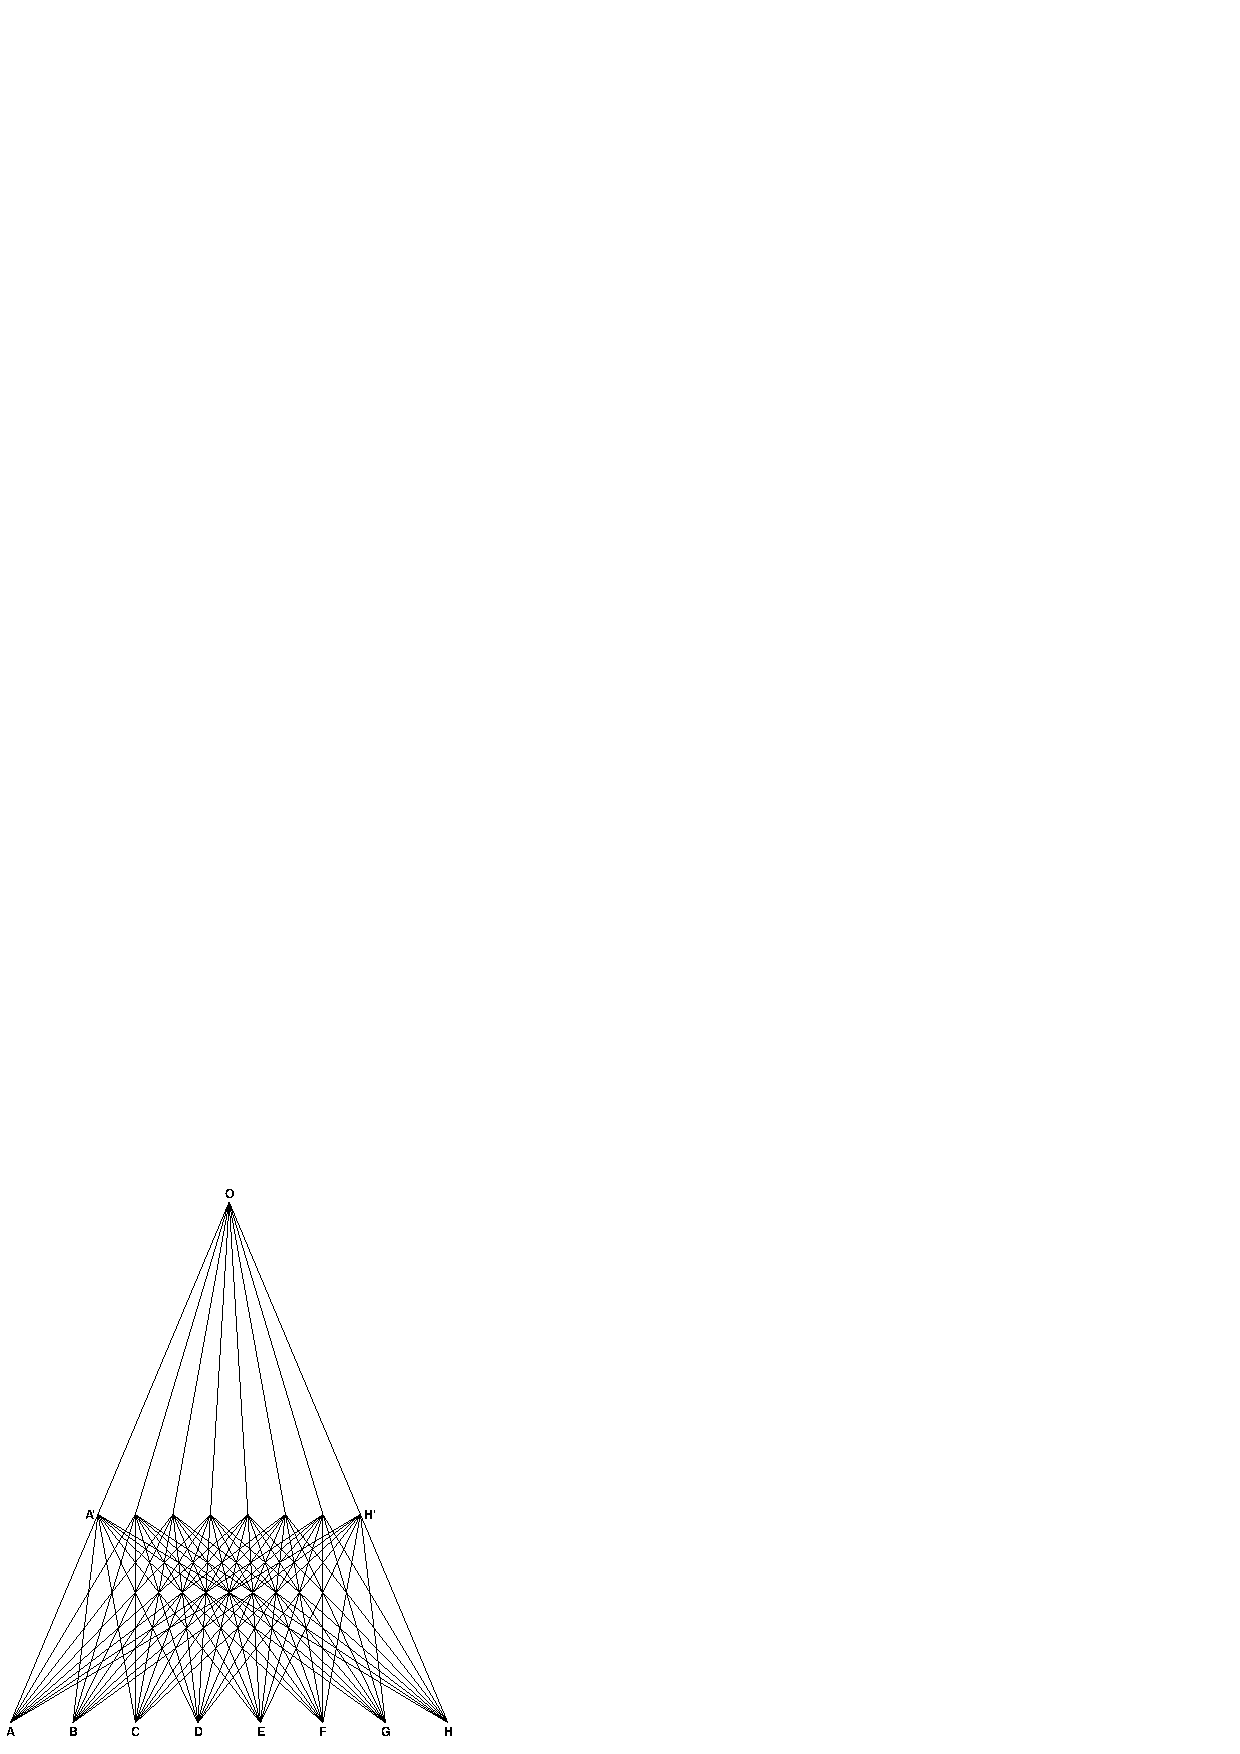
\includegraphics[height=.7\textheight]{./images/illus179}}
\legend{Figure \Uproman{16}}
\DPlabel{figure:xvi}
\end{figure*}

\PG----File: 180.png------------------------------------------------------
The sum of the numbers in each of the 18 lines in
\vhyperlink{figure:xv}{figure~xv} is the same.
To make \vhyperlink{figure:xvi}{figure~xvi} correspond to this we must
number the lines in the pencil $A$ from left to right, $1, 9, \dotsc, 57$,
following the order of the numbers in the first column of the
square: the lines in pencil $B$ must be numbered similarly to
correspond to the numbers in the second column of the square,
and so on. To prevent confusion in the figure I have not
inserted the numbers, but it will be seen that the method of
construction ensures that the sum of the 8 numbers which
designate the lines in each of these 18 pencils is the same.

We can proceed a step further, if the resulting figure is
cut by two other parallel lines perpendicular to the axis, and
if the points of their intersection with the cross-joins be
joined cross-wise, these new cross-joins will intersect on the
axis of the original pencil or on lines perpendicular to it.
The whole figure will now give $8^3$ lines, arranged in $244$ pencils
each of $8$ rays, and will be the reciprocal of a magic cube of
the $8$th order. If we reciprocate back again we obtain a
representation in a plane of a magic cube%
\index{Magic Pencils@\textsc{Magic Pencils}|)}%
\index{Pencils@\textsc{Pencils, Magic}|)}.

\section[Magic Puzzles][Magic Puzzles.]{Magic Square Puzzles}
Many empirical problems, closely
related to magic squares, will suggest themselves; but most of\index
{Magic Square Puzzles|(}
them are more correctly described as ingenious puzzles than
as mathematical recreations. The following will serve as
specimens.

\subsection*{Magic Card Square\protect\footnote
{Ozanam\index{Ozanam@Ozanam's \textit{Récréations}},
1723 edition, vol.~\textsc{iv}, p.~434.}}%
\addcontentsline{toc}{subsection}{Card Square}
The first of these is the familiar
problem of placing the sixteen court cards (taken out of a
pack) in the form of a square so that no row, no column, and
neither of the diagonals shall contain more than one card of
each suit and one card of each rank. The solution presents no
difficulty, and is indicated in figure~xviii \vpageref[below]{figure:xviii}.

\subsection*{Euler's Officers Problem\protect\footnote
{Euler's \textit{Commentationes Arithmeticae}, St~Petersburg, 1849,
vol~\textsc{ii},
pp.~302--361. See also a paper by G.~Tarry\index{Tarry} in the \textit
{Comptes rendus}
of the French Association for the Advancement of Science, Paris, 1900,
vol.~\textsc{ii}, pp.~170--203; and various notes in \textit
{L'Intermédiaire des mathématiciens},
Paris, vol.~\textsc{iii}, 1896, pp.~17, 90; vol.~\textsc{v}, 1898,
pp.~83, 176, 252, % last two digits illegible in scan; these taken from TIA scan of 7th edition
vol.~\textsc{vi}, 1899, p.~251; vol.~\textsc{vii}, 1900, pp.~14, 311.}}%
\addcontentsline{toc}{subsection}{Euler's Officers Problem}
A similar problem, proposed
\PG----File: 181.png------------------------------------------------------
by Euler\index{Euler|(} in 1779, consists in arranging, if it be possible,
thirty-six officers taken from six regiments---the officers being
in six groups, each consisting of six officers of equal rank, one
drawn from each regiment; say officers of rank $a$, $b$, $c$, $d$, $e$, $f$,
drawn from the $1$st, $2$nd, $3$rd, $4$th, $5$th, and $6$th regiments---in
a solid square formation of six by six, so that each row and
each file shall contain one and only one officer of each rank
and one and only one officer from each regiment. The problem
is insoluble.

\subsection*{Extension of Euler's Problem}
More generally\index{Euler|)} we may
investigate the arrangement on a chess-board, containing $n^2$
cells, of $n^2$ counters (the counters being divided into $n$ groups,
each group consisting of $n$ counters of the same colour
numbered consecutively $1, 2, \dotsc, n$) so that each row and each
% [*Note: silently added commas]
column shall contain no two counters of the same colour or
marked with the same number.

For instance, if $n=3$, with three red counters $a_1$, $a_2$, $a_3$,
three white counters $b_1,$ $b_2$, $b_3$, and three black counters
$c_1$, $c_2$, $c_3$,
we can satisfy the conditions by arranging them as in figure~xvii
\vpageref[below]{figure:xviii}.
If $n = 4$, then with counters $a_1$, $a_2$, $a_3$, $a_4$; $b_1$, $b_2$,
$b_3$, $b_4$; $c_1$, $c_2$, $c_3$, $c_4$; $d_1$, $d_2$, $d_3$, $d_4$,
we can arrange them as in
figure~xviii \vpageref[below]{figure:xviii}. A solution when $n = 5$
is indicated in figure~xix.

\begin{figure*}[!hbt]
\centering
\ifPaper\else\hspace*{\fill}\fi
\begin{minipage}[b]{5.5em}
\centering
\begin{MagicSquare}{3}
{a_1} & {b_2} & {c_3} \\
{b_2} & {c_1} & {a_2} \\
{c_3} & {a_3} & {b_1}
\end{MagicSquare}
\legend{Figure \Uproman{17}}
\end{minipage}
\hfill
\begin{minipage}[b]{7em}
\centering
\begin{MagicSquare}{4}
{a_1} & {b_2} & {c_3} & {d_4} \\
{c_4} & {d_3} & {a_2} & {b_1} \\
{d_2} & {c_1} & {b_4} & {a_3} \\
{b_3} & {a_4} & {d_1} & {c_2}
\end{MagicSquare}
\legend{Figure \Uproman{18}}
\end{minipage}
\hfill
\begin{minipage}[b]{8.5em}
\centering
\begin{MagicSquare}{5}
{a_1} & {b_2} & {c_3} & {d_4} & {e_5} \\
{b_5} & {c_1} & {d_2} & {e_3} & {a_4} \\
{c_4} & {d_5} & {e_1} & {a_2} & {b_3} \\
{d_3} & {e_4} & {a_5} & {b_1} & {c_2} \\
{e_2} & {a_3} & {b_4} & {c_5} & {d_1}
\end{MagicSquare}
\legend{Figure \Uproman{19}}
\end{minipage}
\ifPaper\else\hspace*{\fill}\fi
\label{figure:xviii}
\end{figure*}

The problem is soluble if $n$ is odd or if $n$ is of the form
$4m$. If solutions when $n=a$ and when $n=b$ are known, a
\PG----File: 182.png----------------------------------------------------
solution when $n=ab$ can be written down at once. The
theory is closely connected with that of magic squares and
need not be here discussed further.

\subsection*{Magic Domino Squares}%
\addcontentsline{toc}{subsection}{Domino Squares}
Analogous problems can be
made with dominoes\index{Dominoes}. An ordinary set of dominoes, ranging
from double zero to double six, contains $28$ dominoes. Each
domino is a rectangle formed by fixing two small square
blocks together side by side: of these $56$ blocks, eight are
\begin{figure*}[!hbt]
\centering
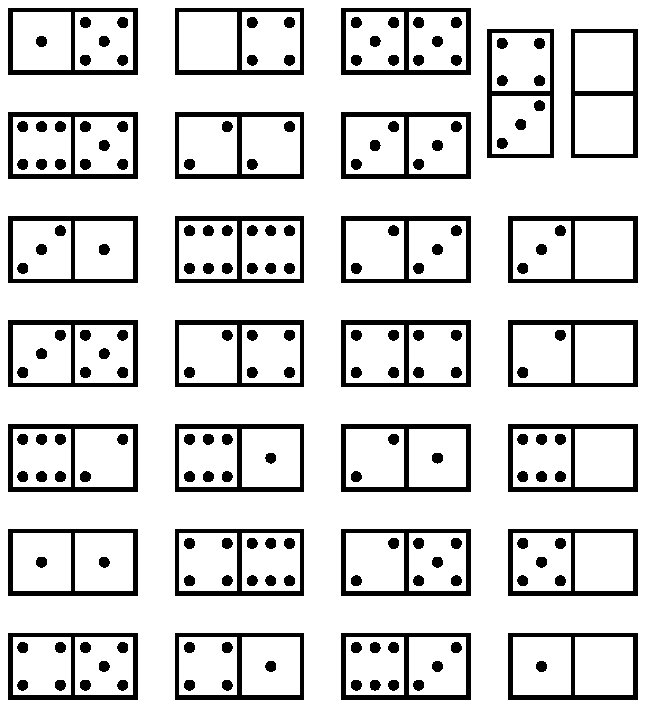
\includegraphics[height=\ifPaper.8\textwidth\else.6\textheight\fi]{./images/illus182}
\legend{Magic Domino Square.}
\label{illus:182}
\end{figure*}
blank, on each of eight of them is one pip, on each of another
eight of them are two pips, and so on. It is required to
arrange the dominoes so that the $56$ blocks form a square of
$7$ by $7$ bordered by one line of $7$ blank squares and so that
the sum of the pips in each row, each column, and in the two
diagonals of the square is equal to $24$. A solution\footnote
{See \textit{L'Illustration}, July~10, 1897.} is given
\vpageref[above]{illus:182}.

Similarly, a set of dominoes, ranging from double zero
to double $n$, contains $\frac{1}{2}(n+1)(n+2)$ dominoes and therefore
\PG----File: 183.png----------------------------------------------------
$(n+1)(n+2)$ blocks. Can these dominoes be arranged in the
form of a square of $(n+1)^2$ cells, bordered by a row of blanks,
so that the sum of the pips in each row, each column, and in
the two diagonals of the square is equal to $\frac{1}{2}n(n+2)$?

\subsection*{Magic Coin Squares\protect\footnote
{See \textit{The Strand Magazine}, London, December, 1896, pp.~720, 721.
}}\addcontentsline{toc}{subsection}{Coin Squares}
There are somewhat similar questions
concerned with coins. Here is one applicable to a
square of the third order divided into nine cells, as in figure~xvii
\ifPaper\vpageref[above]{figure:xviii}\else\vpageref{figure:xviii}\fi. % [*Note: originally "above"]
% In print mode, vpageref gets into an infinite loop here (there is always a "labels have changed warning")
If a five-shilling piece is placed in the middle
cell $c_1$ and a florin in the cell below it, namely, in $a_3$ it is
required to place the fewest possible current English coins in
the remaining seven cells so that in each cell there is at least
one coin, so that the total value of the coins in every cell is
different, and so that the sum of the values of the coins in
each row, column, and diagonal is fifteen shillings: it will be
found that thirteen additional coins will suffice. A similar
problem is to place ten current English postage stamps, all but
two being different, in the nine cells so that the sum of the
values of the stamps in each row, column, and diagonal is
ninepence.\index{Magic Square Puzzles|)}


\PG----File: 184.png----------------------------------------------------
%CHAPTER VI.

\chapter{Unicursal Problems.}

\textsc{I propose} to consider in this chapter some problems which\chapindex
{Unicursal Problems@\textsc{Unicursal Problems}}
arise out of the theory of unicursal curves. I shall commence
with \emph{Euler's Problem and Theorems}, and shall apply the
results briefly to the theories of \emph{Mazes} and \emph{Geometrical Trees}.
The reciprocal unicursal problems of the \emph{Hamilton Game} and
the \emph{Knight's Path on a Chess-board} will be discussed in the
latter half of the chapter.

\section{Euler's Problem} Euler's problem%
\index{Euler'sUni@\textsc{Euler's Unicursal Problem}|(}%
\index{Konigsberg@Königsberg Problem|(}
has its origin in a memoir\footnote
{\textit{Solutio problematis ad Geometriam situs pertinentis},
\textit{Commentarii
Academiae Scientiarum Petropolitanae} for 1736, St~Petersburg, 1741,
vol.~\textsc{viii}, pp.~128--140. This has been translated into French
by M.~Ch.~Henry\index{Henry on Unicursal Problems};
see Lucas\index{Lucas, E.}, vol.~\textsc{i}, part~2, pp.~21--33.
} presented by him in 1736 to the St~Petersburg
Academy, in which he solved a question then under discussion
as to whether it was possible to take a walk in the town of
Königsberg in such a way as to cross every bridge in it once
and only once.

The town is built near the mouth of the river Pregel,
which there takes the form indicated \vpageref[below]{illus:185a}
and includes the
%[*Note: Illustration moved from 185.png to improve screen version]
\begin{figure*}[!hbt]
\centerline{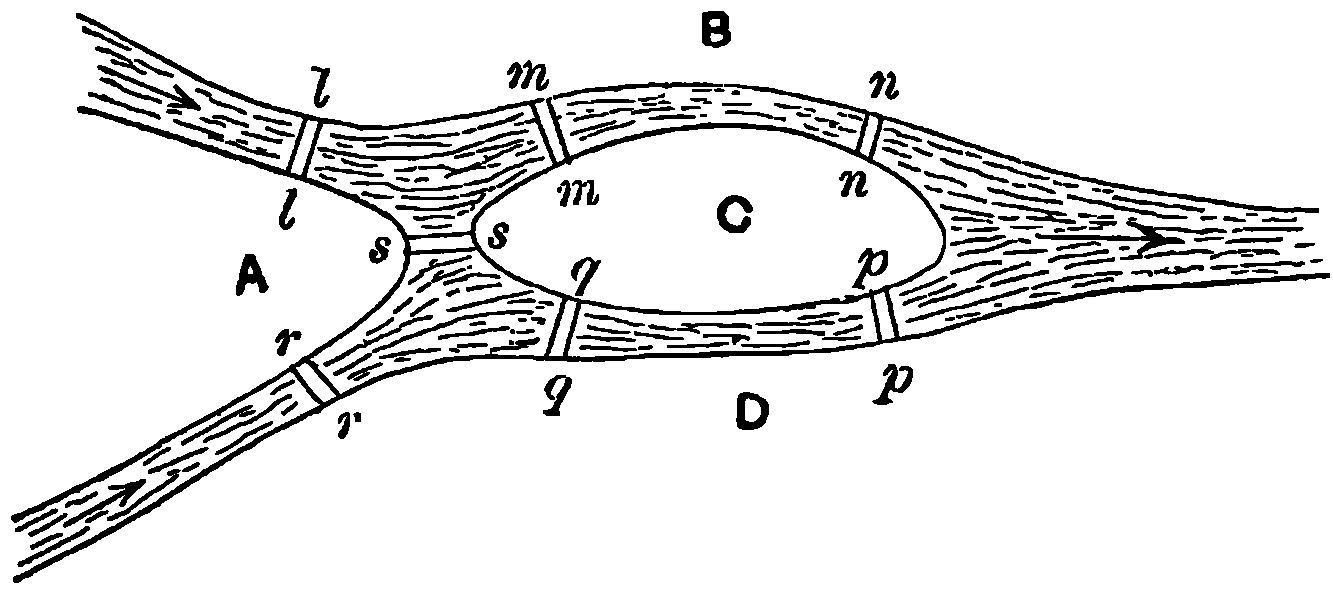
\includegraphics[width=.8\textwidth]{./images/illus185a}}
\label{illus:185a}
\end{figure*}
island of Kneiphof. In 1759 there were (and according to
Baedeker there are still) seven bridges in the positions shown
in the diagram, and it is easily seen that with such an
arrangement the problem is insoluble. Euler however did not
\PG----File: 185.png----------------------------------------------------
confine himself to the case of Königsberg, but discussed the
general problem of any number of islands connected in any
way by bridges. It is evident that the question will not be
affected if we suppose the islands to diminish to points and
the bridges to lengthen out. In this way we ultimately obtain
a geometrical figure or network. In the Königsberg problem
this figure is of the shape indicated \vpageref[below]{illus:185b},
the areas being
represented by the points $A$, $B$, $C$, $D$, and the bridges being
represented by the lines $l$, $m$, $n$, $p$, $q$, $r$, $s$.

\begin{figure*}[!hbt]
\centerline{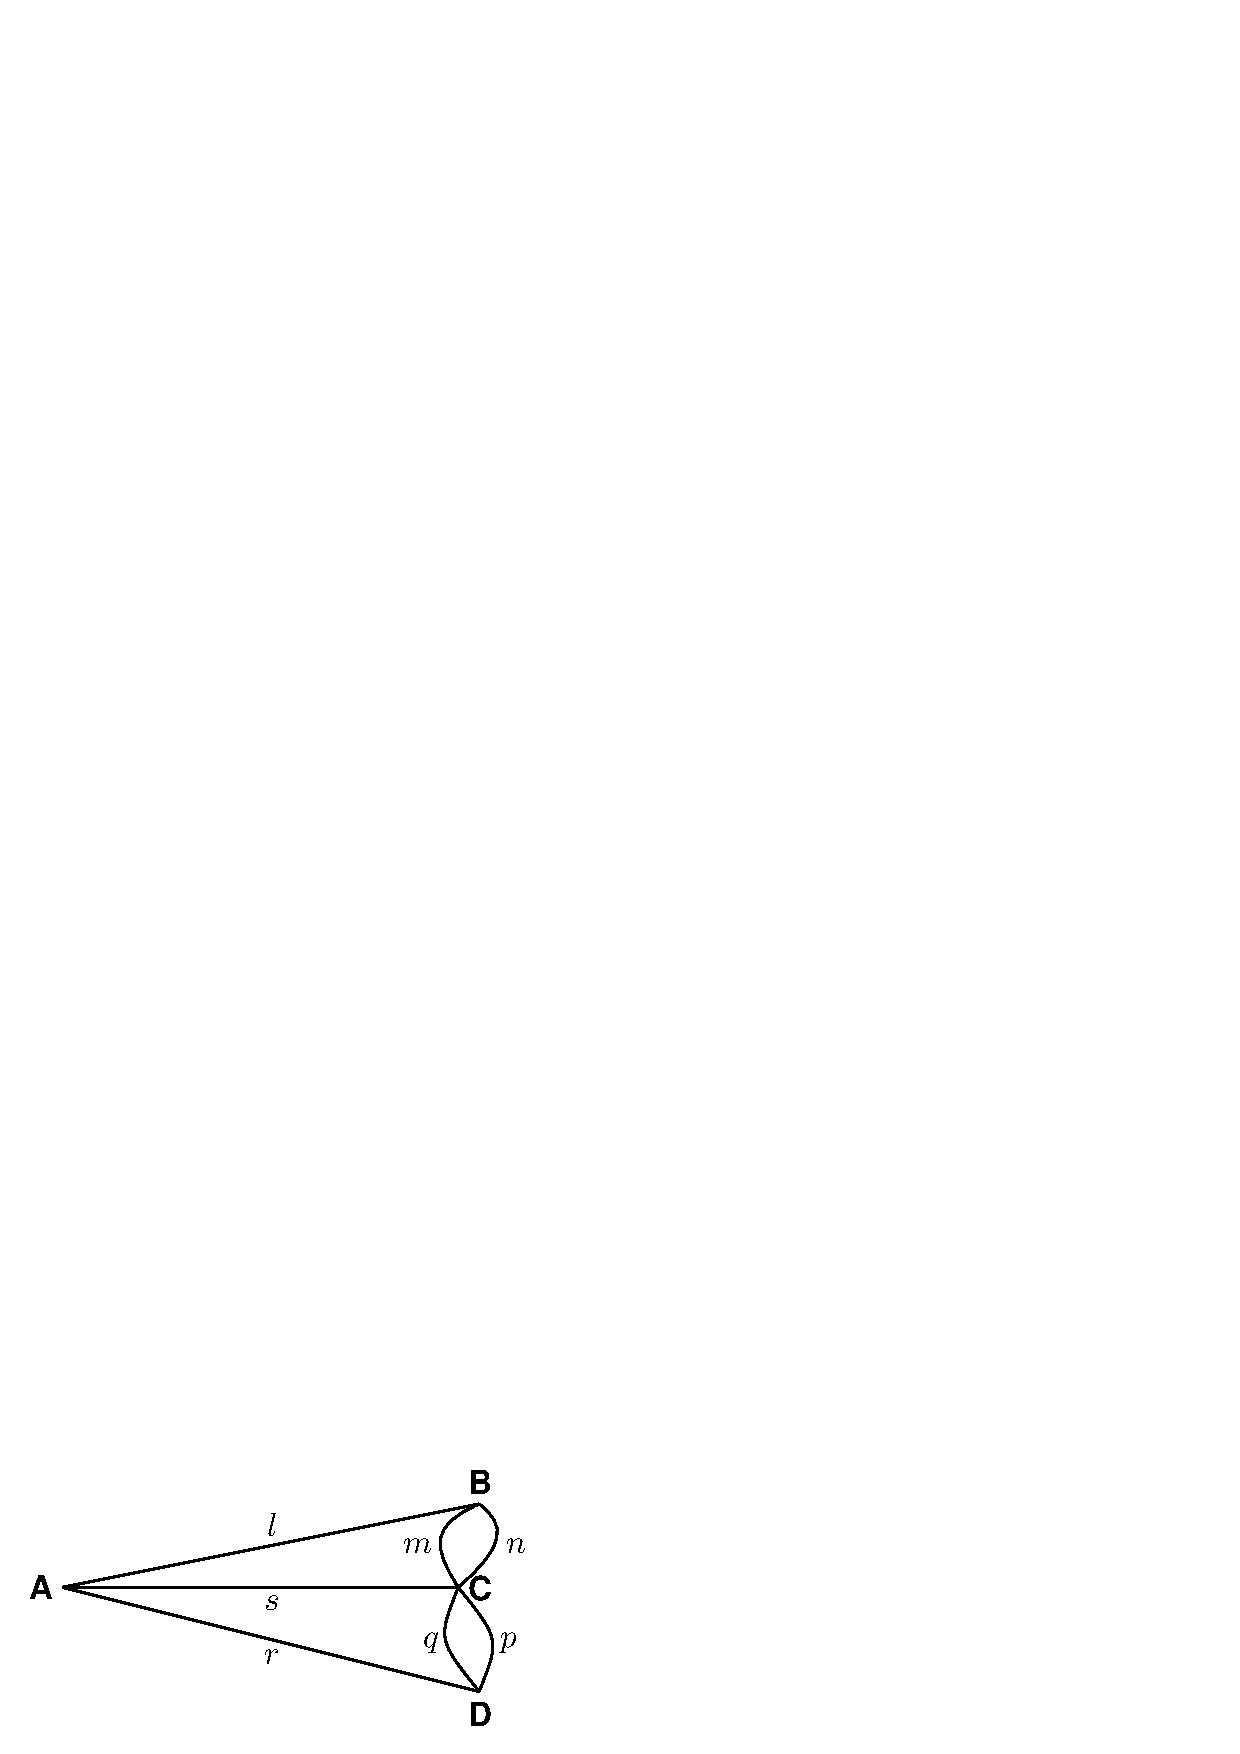
\includegraphics[width=.6\textwidth]{./images/illus185b}}
\label{illus:185b}
\end{figure*}

Euler's problem consists therefore in finding whether a
given geometrical figure can be described by a point moving
so as to traverse every line in it once and only once. A more
general question is to determine how many strokes are necessary
to describe such a figure so that no line is traversed
twice: this is covered by the rules hereafter given. The
figure may be either in three or in two dimensions, and
it may be represented by lines, straight, curved, or tortuous,
\PG----File: 186.png----------------------------------------------------
joining a number of given points, or a model may be
constructed by taking a number of rods or pieces of string
furnished at each end with a hook so as to allow of any
number of them being connected together at one point.

The theory of such figures is included as a particular case
in the propositions proved by Listing\index
{Listing@Listing's \textit{Topologie}} in his \textit{Topologie}\footnote
{\textit{Die Studien}, Göttingen, 1847, part~x. See also Tait\index
{Tait} on \textit{Listing's Topologie},
\textit{Philosophical Magazine}, London, January, 1884, series~5,
vol.~\textsc{xvii}, pp.~30--46.}. I
shall, however, adopt here the methods of Euler, and I shall
begin by giving some definitions, as it will enable me to put
the argument in a more concise form.

\phantomsection
\addcontentsline{toc}{subsection}{Definitions}
A \emph{node} (or isle) is a point to or from which lines are
drawn. A \emph{branch} (or bridge or path) is a line connecting
two consecutive nodes. An \emph{end} (or hook) is the point at
each termination of a branch. The \emph{order} of a node is the
number of branches which meet at it. A node to which only
one branch is drawn is a \emph{free} node or a free end. A node
at which an even number of branches meet is an \emph{even} node:
evidently the presence of a node of the second order is immaterial.
A node at which an odd number of branches meet
is an \emph{odd} node. A figure is closed if it has no free end:
such a figure is often called a closed network.

A \emph{route} consists of a number of branches taken in consecutive
order and so that no branch is traversed twice. A
closed % [*Note: silently correcting obvious typo "close"]
route terminates at the point from which it started.
A figure is described \emph{unicursally} when the whole of it is
traversed in one route.

\phantomsection
\addcontentsline{toc}{subsection}{Euler's Theorems}
The following are Euler's results. (i)~In a closed network
the number of odd nodes is even. (ii)~A figure which
has no odd node can be described unicursally, in a re-entrant
route, by a moving point which starts from any point on it.
(iii)~A figure which has two and only two odd notes can be
described unicursally by a moving point which starts from one
of the odd nodes and finishes at the other. (iv)~A figure
which has more than two odd nodes cannot be described
\PG----File: 187.png------------------------------------------------------
completely in one route; to which Listing\index
{Listing@Listing's \textit{Topologie}} added the corollary
that a figure which has $2n$ odd nodes, and no more, can
be described completely in $n$ separate routes. I now proceed
to prove these theorems.

\subsection*{First} \emph{The number of odd nodes in a closed network is
even.}

Suppose the number of branches to be $b$. Therefore the
number of hooks is $2b$. Let $k_n$ be the number of nodes of
the $n$th order. Since a node of the $n$th order is one at
which $n$ branches meet, there are $n$ hooks there. Also since
the figure is closed, $n$ cannot be less than $2$.
\[\def\tabcolsep{0pt}
\begin{tabularx}{\textwidth}{XrrrlX}
& $\Therefore 2k_2 +{}$& $3k_3 +{}$& $4k_4 + \dotsb $&${} + nk_n
+ \dotsb = 2b\,.$& \\
  Hence & &    $ 3k_3 +{}$&$ 5k_5 + \dotsb $& \quad is even.  \\
& $\Therefore$       & $ k_3+{}$&$   k_5 + \dotsb $& \quad is even.
\end{tabularx}
\]

\subsection*{Second} \emph{A figure which has no odd node can be described
unicursally in a re-entrant route.}

Since the route is to be re-entrant it will make no difference
where it commences. Suppose that we start from a node
$A$. Every time our route takes us through a node we use
up one hook in entering it and one in leaving it. There
are no odd nodes, therefore the number of hooks at every
node is even: hence, if we reach any node except $A$, we
shall always find a hook which will take us into a branch
previously untraversed. Hence the route will take us finally
to the node $A$ from which we started. If there are more than
two hooks at $A$, we can continue the route over one of the
branches from $A$ previously untraversed, but in the same way
as before we shall finally come back to $A$.

It remains to show that we can arrange our route so as
to make it cover all the branches. Suppose each branch of
the network to be represented by a string with a hook at each
end, and that at each node all the hooks there are fastened
together. The number of hooks at each node is even, and if
\PG----File: 188.png----------------------------------------------------
they are unfastened they can be re-coupled together in pairs,
the arrangement of the pairs being immaterial. The whole
network will then form one or more closed curves, since now
each node consists merely of two ends hooked together.

If this random coupling gives us one single curve then the
proposition is proved; for starting at any point we shall go
along every branch and come back to the initial point. But if
this random coupling produces anywhere an isolated loop, $L$,
then where it touches some other loop, $M$, say at the node $P$,
unfasten the four hooks there (viz.\ two of the loop $L$ and two
of the loop $M$) and re-couple them in any other order: then
the loop $L$ will become a part of the loop $M$. In this way, by
altering the couplings, we can transform gradually all the
separate loops into parts of only one loop.

For example, take the case of three isles, $A$, $B$, $C$, each
connected with both the others by two bridges. The most
unfavourable way of re-coupling the ends at $A$, $B$, $C$ would be
to make $ABA$, $ACA$, and $BCB$ separate loops. The loops
$ABA$ and $ACA$ are separate and touch at $A$; hence we should
re-couple the hooks at $A$ so as to combine $ABA$ and $ACA$ into
\begin{figure*}[!hbt]
\centerline{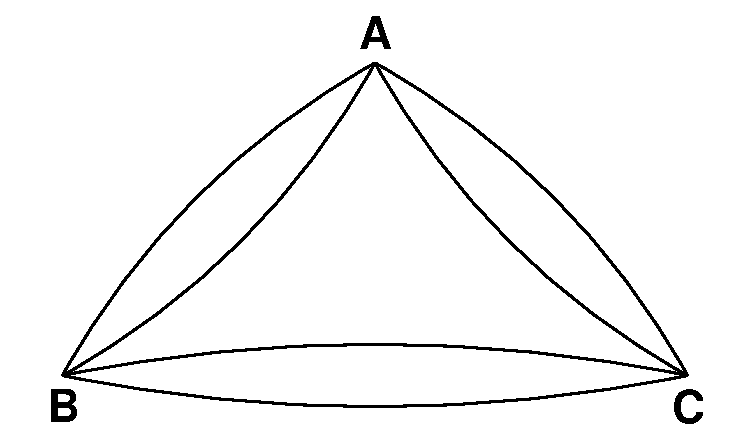
\includegraphics[width=7cm]{./images/illus188}}
\end{figure*}
one loop $ABACA$. Similarly, by re-arranging the couplings of
the four hooks at $B$, we can combine the loop $BCB$ with
$ABACA$ and thus make only one loop.

I infer from Euler's language that he had attempted to
solve the problem of giving a practical rule which would enable
one to describe such a figure unicursally without knowledge of
\PG----File: 189.png----------------------------------------------------
its form, but that in this he was unsuccessful. He however
added that any geometrical figure can be described completely
in a single route provided each part of it is described twice and
only twice, for, if we suppose that every branch is duplicated,
there will be no odd nodes and the figure is unicursal. In
this case any figure can be described completely without knowing
its form: rules to effect this are given below.

\subsection*{Third} \emph{A figure which has two and only two odd nodes can
be described unicursally by a point which starts from one of
the odd nodes and finishes at the other odd node.}

This at once reduces to the second theorem. Let $A$ and $Z$
be the two odd nodes. First, suppose that $Z$ is not a free
end. We can, of course, take a route from $A$ to $Z$; if we
imagine the branches in this route to be eliminated, it will
remove one hook from $A$ and make it even, will remove two
hooks from every node intermediate between $A$ and $Z$ and
therefore leave each of them even, and will remove one hook
from $Z$ and therefore will make it even. All the remaining
network is now even: hence, by Euler's second proposition,
it can be described unicursally, and, if the route begins at
$Z$, it will end at $Z$. Hence, if these two routes are taken
in succession, the whole figure will be described unicursally,
beginning at $A$ and ending at $Z$. Second, if $Z$ is a free
end, then we must travel from $Z$ to some node, $Y$, at which
more than two branches meet. Then a route from $A$ to $Y$
which covers the whole figure exclusive of the path from $Y$
to $Z$ can be determined as before and must be finished by
travelling from $Y$ to $Z$.

\subsection*{Fourth} \emph{A figure having $2n$ odd nodes, and no more, can
be described completely in $n$ separate routes.}

If any route starts at an odd node, and if it is continued
until it reaches a node where no fresh path is open to it, this
latter node must be an odd one. For every time we enter
an even node there is necessarily a way out of it; and similarly
every time we go through an odd node we use up one hook in
entering and one hook in leaving, but whenever we reach it as
\PG----File: 190.png----------------------------------------------------
the end of our route we use only one hook. If this route is
suppressed there will remain a figure with $2n-2$ odd nodes.
Hence $n$ such routes will leave one or more networks with
only even nodes. But each of these must have some node
common to one of the routes already taken and therefore can
be described as a part of that route. Hence the complete
passage will require n and not more than $n$ routes. It follows,
as stated by Euler, that, if there are more than two odd
nodes, the figure cannot be traversed completely in one
route.

\phantomsection
\addcontentsline{toc}{subsection}{Examples}
The Königsberg bridges lead to a network with four odd
nodes; hence, by Euler's fourth proposition, it cannot be
described unicursally in a single journey, though it can be
traversed completely in two separate routes.

The first and second diagrams figured \vpageref[below]{illus:190} contain
only even nodes, and therefore each of them can be described unicursally.
\begin{figure*}[!hbt]
\centerline{\ifpdf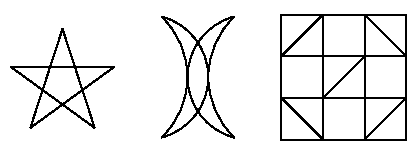
\includegraphics[width=\ifPaper\else.7\fi\textwidth,viewport=0 0 200 70]{./images/illus190.pdf} % size graphic using BoundingBox
\else\includegraphics[width=\ifPaper\else.7\fi\textwidth]{./images/illus190.eps}\fi}
\label{illus:190}
\end{figure*}
The first of these---a re-entrant pentagon---was one
of the Pythagorean symbols\index{Pythagorean Symbol}.
The other is the so-called sign-manual of Mohammed\index
{Mohammed's sign-manual}, said to have been originally traced
in the sand by the point of his scimetar without taking the
scimetar off the ground or retracing any part of the figure---which,
as it contains only even nodes, is possible. The third
diagram is taken from Tait's\index{Tait} article: it contains only two
odd nodes, and therefore can be described unicursally if we
start from one of them and finish at the other.

As other examples I may note that the geometrical figure
\PG----File: 191.png----------------------------------------------------
formed by taking a $(2n+1)$gon and joining every angular
point with every other angular point is unicursal. On the
other hand a chess-board, divided as usual by straight lines
into $64$ cells, has $28$ odd nodes and $53$ even nodes: hence it
would require $14$ separate pen-strokes to trace out all the
boundaries without going over any more than once. Again,
the diagram on page \pageref{illus:136} has $20$ odd nodes and therefore
would require $10$ separate pen-strokes to trace it out.

It is well known that a curve which has as many nodes as
is consistent with its degree is unicursal.

\section[Mazes][Mazes and Labyrinths.]{Mazes}
Everyone has read of the labyrinth\index
{Labyrinths|(} of Minos\index{Minos} in
Crete and of Rosamund's Bower. A few modern mazes\index{Mazes|(} exist
here and there---notably one, which is a very poor specimen
of its kind, at Hampton Court\index{Hampton Court, Maze at}---and
in one of these, or at any
rate on a drawing of one, most of us have threaded our way
to the interior. I proceed now to consider the manner in
which any such construction may be completely traversed even
by one who is ignorant of its plan.

The theory of the description of mazes is included in
Euler's theorems given above. The paths in the maze are
what previously we have termed branches, and the places
where two or more paths meet are nodes. The entrance to
the maze, the end of a blind alley, and the centre of the maze
are free ends and therefore odd nodes.

If the only odd nodes are the entrance to the maze and the
centre of it--which will necessitate the absence of all blind
alleys--the maze can be described unicursally. This follows
from Euler's third proposition. Again, no matter how many
odd nodes there may be in a maze, we can always find a
route which will take us from the entrance to the centre
without retracing our steps, though such a route will take us
through only a part of the maze. But in neither of the cases
mentioned in this paragraph can the route be determined
without a plan of the maze.

A plan is not necessary, however, if we make use of
\PG----File: 192.png----------------------------------------------------
Euler's suggestion, and suppose that every path in the maze
is duplicated. In this case we can give definite rules for the
complete description of the whole of any maze, even if we are
entirely ignorant of its plan. Of course to walk twice over
every path in a labyrinth is not the shortest way of arriving
at the centre, but, if it is performed correctly, the whole maze
is traversed, the arrival at the centre at some point in the
course of the route is certain, and it is impossible to lose one's
way\index{Euler'sUni@\textsc{Euler's Unicursal Problem}|)}%
\index{Konigsberg@Königsberg Problem|)}.

\phantomsection
\addcontentsline{toc}{subsection}{Rules for completely traversing a Maze}
I need hardly explain why the complete description of such
a duplicated maze is possible, for now every node is even,
and hence, by Euler's second proposition, if we begin at the
entrance we can traverse the whole maze; in so doing we
shall at some point arrive at the centre, and finally shall
emerge at the point from which we started. This description
will require us to go over every path in the maze twice, and as
a matter of fact the two passages along any path will be always
made in opposite directions.

If a maze is traced on paper, the way to the centre is
generally obvious, but in an actual labyrinth it is not so easy
to find the correct route unless the plan is known. In order
to make sure of describing a maze without knowing its plan it
is necessary to have some means of marking the paths which
we traverse and the direction in which we have traversed them---for
example, by drawing an arrow at the entrance and end of
every path traversed, or better perhaps by marking the wall on
the right-hand side, in which case a path may not be entered
when there is a mark on each side of it. If we can do this,
and if when a node is reached, we take, if it be possible, some
path not previously used, or, if no other path is available, we
enter on a path already traversed once only, we shall completely
traverse any maze in two dimensions\footnote
{See \textit{Le problème des labyrinthes} by G.~Tarry\index{Tarry},
\textit{Nouvelles Annales de
math\-é\-mat\-iques}, May, 1895, series~3, vol.~\textsc{xiv}.
}. Of course a
path must not be traversed twice in the same direction, a
\PG----File: 193.png----------------------------------------------------
path already traversed twice (namely, once in each direction)
must not be entered, and at the end of a blind alley it is
necessary to turn back along the path by which it was
reached.

\phantomsection
\addcontentsline{toc}{subsection}{Notes on the History of Mazes}
I think most people would understand by a maze a series of
interlacing paths through which some route can be obtained
leading to a space or building at the centre of the maze. I
believe that few, if any, mazes of this type existed in classical
or medieval times.

One class of what the ancients called mazes or labyrinths
seems to have comprised any complicated building with numerous
vaults and passages\footnote
{For instance, see the descriptions of the labyrinth at Lake Moeris
given by Herodotus\index{Herodotus on Lake Moeris}, bk.~ii, c.~148;
Strabo\index{Strabo on Lake Moeris}, bk.~xvii, c.~1, art.~37;
Diodorus\index{Diodorus on Lake Moeris}, bk.~i, cc.~61, 66; and
Pliny\index{Pliny}, \textit{Hist. Nat.}, bk.~xxxvi, c.~13, arts.~84--89.
On these and other references see A.~Wiedemann\index
{Wiedemann on Lake Moeris}, \textit{Herodots
zweites Buch}, Leipzig, 1890, p.~522 \etseq\ See also Virgil\index{Virgil},
\textit{Aeneid}, bk.~v,
c.~v, 588; Ovid\index{Ovid}, \textit{Met.}, bk.~viii, c.~5, 159; % silently correcting viii. to viii,
Strabo, bk.~viii, c.~6.}. Such a building might be termed a
labyrinth, but it is not what is usually understood by the word.
The above rules would enable anyone to traverse the whole of
any structure of this kind. I do not know if there are any
accounts or descriptions of Rosamund's Bower\index{Rosamund's Bower}
other than those
by Drayton\index{Drayton}, Bromton\index{Bromton}, and Knyghton\index
{Knyghton}: in the opinion of some,
these imply that the bower was merely a house, the passages
in which were confusing and ill-arranged.

Another class of ancient mazes consisted of a tortuous path
confined to a small area of ground and leading to a place or
shrine in the centre\footnote
{On ancient and medieval labyrinths---particularly of this kind---see
an article by Mr~E.~Trollope\index{Trollope on Mazes} in \textit
{The Archaeological Journal}, 1858, vol.~\textsc{xv},
pp.~216--235, from which much of the historical information given above
is derived}. This is a maze in which there is no
chance of taking a wrong turning; but, as the whole area
can be occupied by the windings of one path, the distance
to be traversed from the entrance to the centre may be
considerable, even though the piece of ground covered by the
maze is but small.

\PG----File: 194.png----------------------------------------------------
The traditional form of the labyrinth\index
{Cretan Labyrinth}\index{Daedalus, Labyrinth of} constructed for
the Minotaur\index{Minotaur} is a specimen of this class. It was delineated
on the reverses of the coins of Cnossus\index{Cnossus, Coins of},
specimens of which
are not uncommon; one form of it is indicated in the
\vpageref[accompanying diagram][diagram ]{illus:194}
(figure~i). The design really is the
same as that drawn in figure~ii, as can be easily seen by
bending round a circle the rectangular figure there given.

Mr~Inwards\index{Inwards on the Cretan Maze} has suggested\footnote
{\textit{Knowledge}, London, October, 1892.} that this design on the coins
of Cnossus may be a survival from that on a token given by
\begin{figure*}[!hbt]
\centering
\begin{minipage}{.3\textwidth}
\centerline{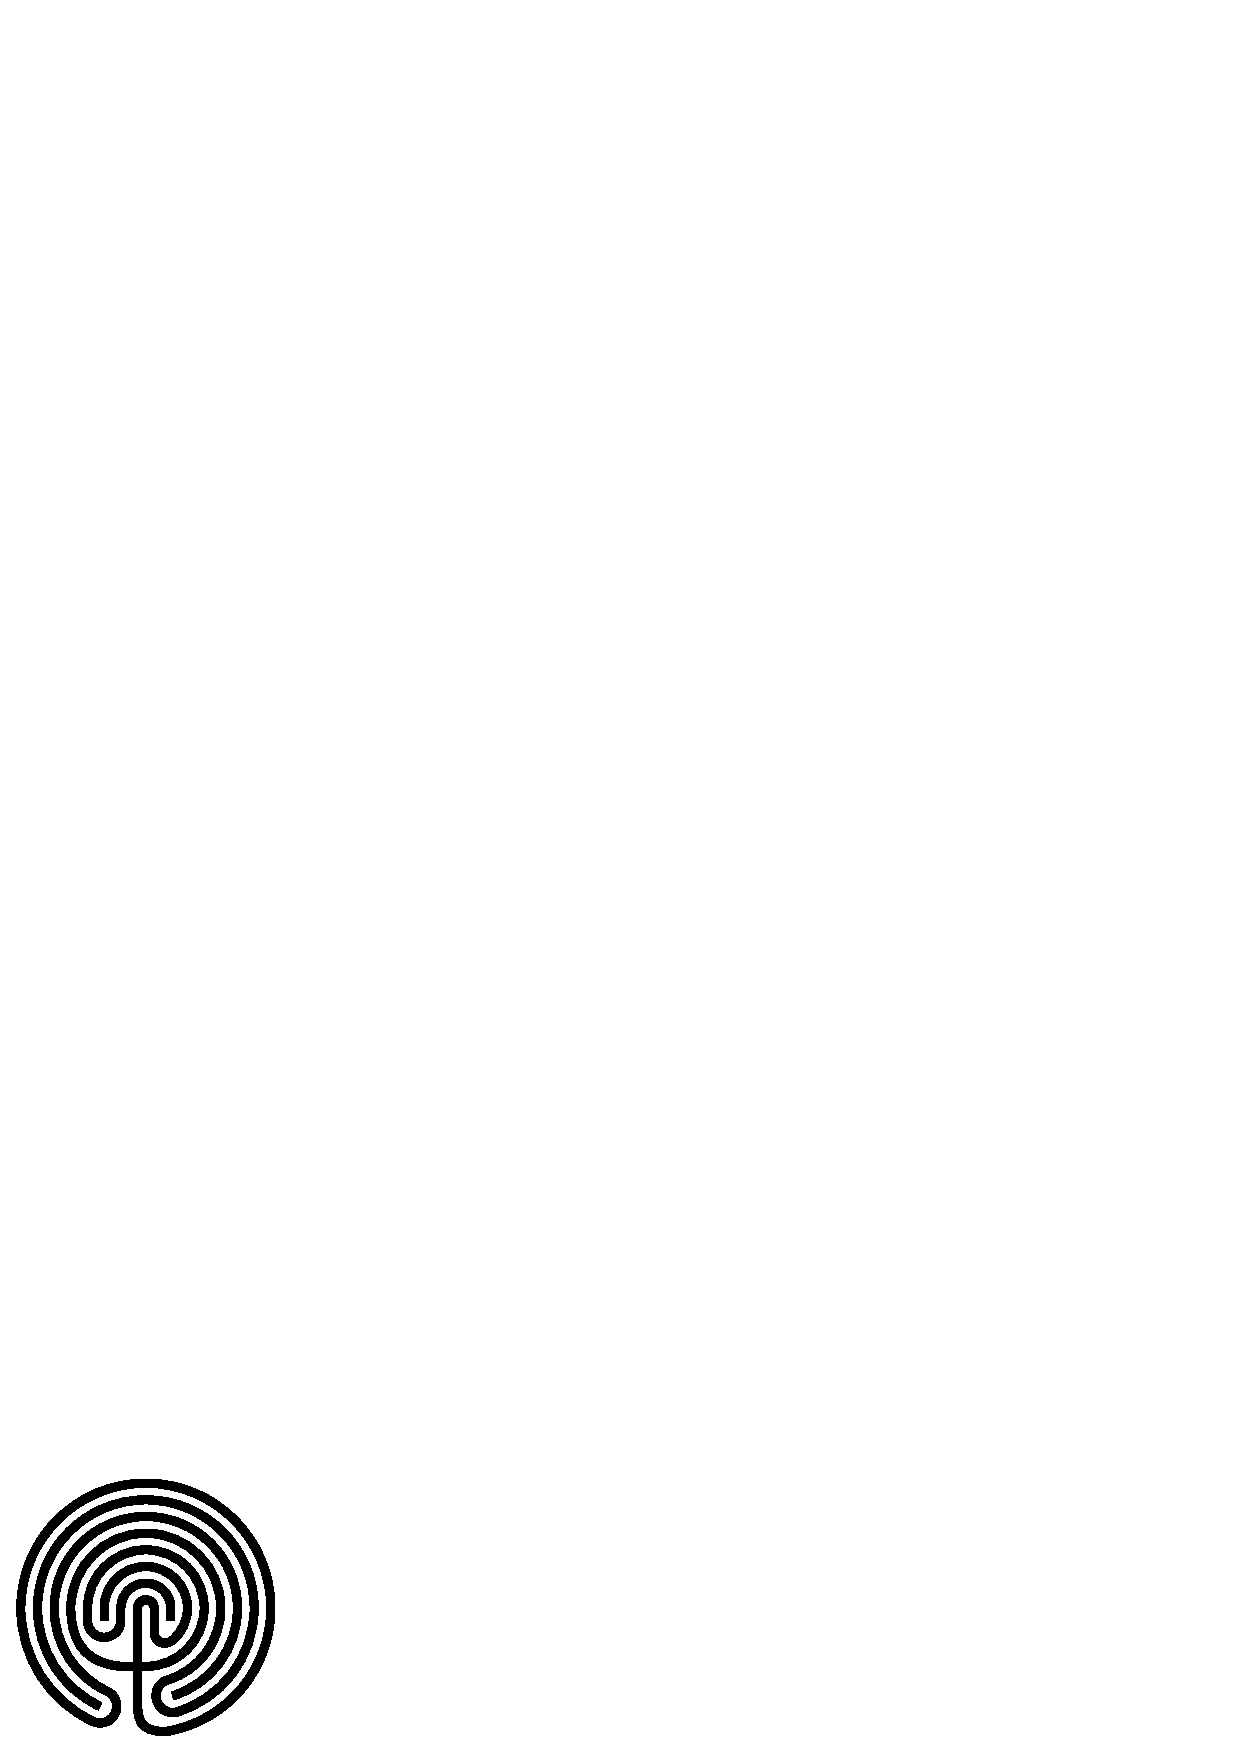
\includegraphics[width=\textwidth]{./images/illus194a}}
\legend{Figure \Uproman{1}}
\end{minipage}
\hfill
\begin{minipage}{.6\textwidth}
\centerline{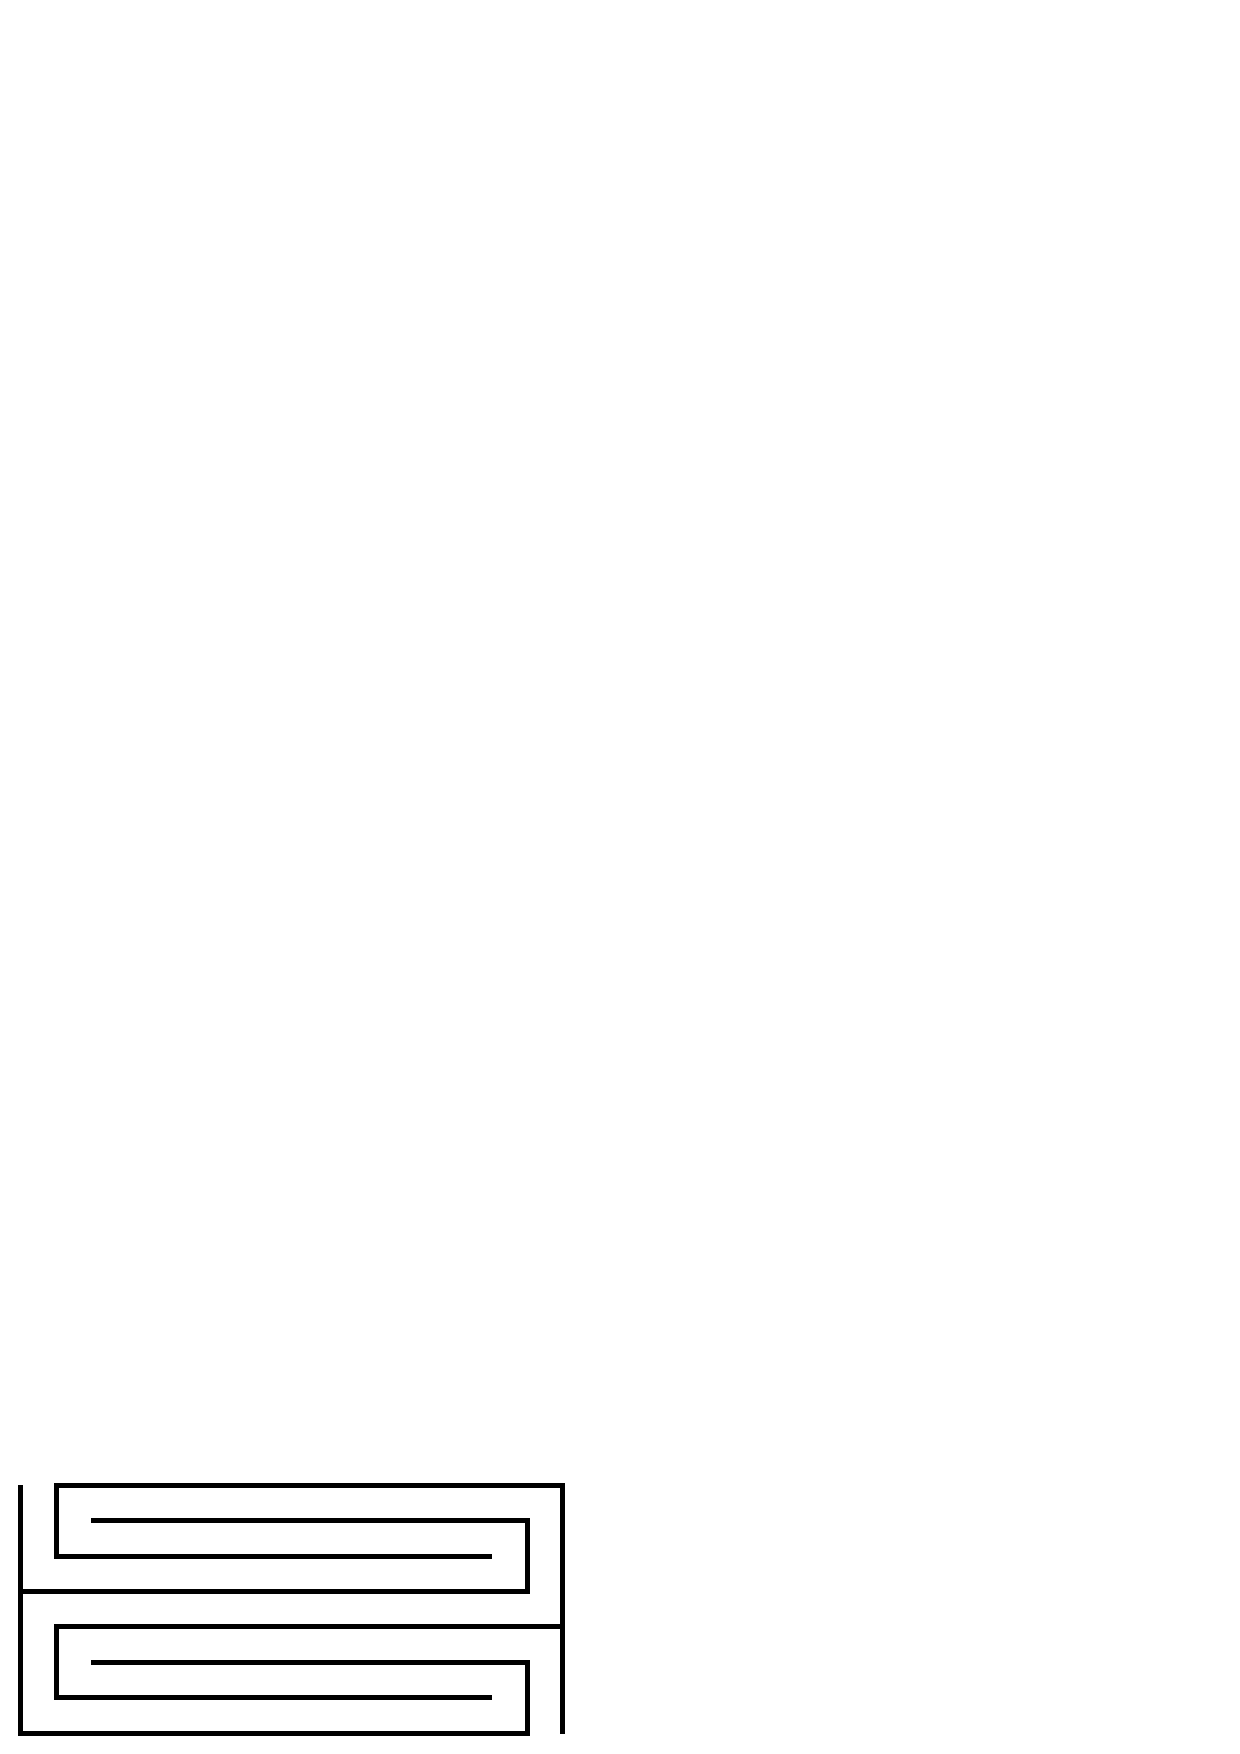
\includegraphics[width=\textwidth]{./images/illus194b}}
\legend{Figure \Uproman{2}}
\end{minipage}
\label{illus:194}
\end{figure*}
the priests as a clue to the right path in the labyrinth there.
Taking the circular form of the design shown above he supposed
each circular wall to be replaced by two equidistant
walls separated by a path, and thus obtained a maze to which
the original design would serve as the key. The route thus
indicated may be at once obtained by noticing that when a
node is reached (\IE\ a point where there is a choice of paths)
the path to be taken is that which is next but one to that by
which the node was approached. This maze may be also
threaded by the simple rule of always following the wall on
the right-hand side or always that on the left-hand side.
The labyrinth may be somewhat improved by erecting a few
additional barriers, without affecting the applicability of the
above rules, but it cannot be made really difficult. This
makes a pretty toy, but though the conjecture on which it is
founded is ingenious it must be regarded as exceedingly
\PG----File: 195.png---------------------------------------------------
improbable. Another suggestion is that the curved line on
the reverse of the coins indicated the form of the rope held
by those taking part in some rhythmic dance; while others
consider that the form was gradually evolved from the widely
prevalent svastika\index{Svastika}.

Copies of the maze of Cnossus were frequently engraved
on Greek and Roman gems; similar but more elaborate
designs are found in numerous Roman mosaic pavements\index
{Mosaic Pavements}\footnote
{See \Eg\ Breton's\index{Breton on Mosaics} \textit{Pompeia}, p.~303.}.
A copy of the Cretan labyrinth\index{Cretan Labyrinth} was embroidered
on many of
the state robes of the later Emperors, and, apparently thence,
was copied on to the walls and floors of various churches\footnote
{Ozanam\index{Ozanam, A.F., on Labyrinths}, \textit
{Graphia aureae urbis Romae}, pp.~92, 178.}.
At a later time in Italy and in France these mural and pavement
decorations were developed into scrolls of great complexity,
but consisting, as far as I know, always of a single
line. Some of the best specimens now extant are on the walls
of the cathedrals at Lucca\index{Lucca, Labyrinth at}, Aix\index
{Aix, Labyrinth at} in Provence, and Poitiers\index{Poitiers, Labyrinth at};
and on the floors of the churches of Santa Maria in Trastevere\index
{Trastevere, Labyrinth at}
at Rome\index{Rome, Labyrinth at}, San~Vitale at Ravenna\index
{Ravenna, Labyrinth at}, Notre Dame at St~Omer\index
{StOmer@St Omer, Labyrinth at},
and the cathedral at Chartres\index{Chartres, Labyrinth at}.
It is possible that they were
used to represent the journey through life as a kind of pilgrim's
progress.

In England these mazes were usually, perhaps always, cut
in the turf adjacent to some religious house or hermitage: and
there are some slight reasons for thinking that, when traversed
as a religious exercise, a \emph{pater} or \emph{ave} had to be repeated at
every turning. After the Renaissance, such labyrinths were
frequently termed Troy-towns\index{Troy-towns} or Julian's bowers\index
{Julian's Bowers}. Some
of the best specimens, which are still extant, are those
at Rockliff Marshes\index{Rockliff Marshes, Labyrinth at}, Cumberland;
Asenby\index{Asenby, Labyrinth at}, Yorkshire;
Alkborough\index{Alkborough, Labyrinth at}, Lincolnshire;
Wing\index{Wing, Labyrinth at}, Rutlandshire;
Boughton-Green\index{Boughton Green, Labyrinth at}, Northamptonshire;
Comberton\index{Comberton, Labyrinth at}, Cambridgeshire;
Saffron Walden\index{Saffron Walden, Labyrinth at}, Essex;
and Chilcombe\index{Chilcombe, Labyrinth at}, near Winchester.

The modern maze seems to have been introduced---probably
from Italy---during the Renaissance, and many of the
\PG----File: 196.png-----------------------------------------------------
palaces and large houses built in England during the Tudor
and the Stuart periods had labyrinths attached to them.
Those adjoining the royal palaces at Southwark\index
{Southwark, Labyrinth at}, Greenwich\index{Greenwich, Labyrinth at},
and Hampton Court\index{Hampton Court, Maze at} were particularly well
known from their
vicinity to the capital. The last of these was designed by
London and Wise\index{London and Wise} in 1690, for William~III\index
{William III of England}, who had a fancy
for such conceits: a plan of it is given in various guide-books.
\begin{figure*}[!hbt]
\centerline{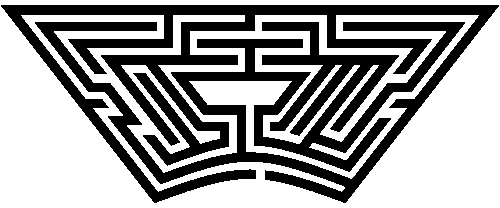
\includegraphics[width=\ifPaper.8\else.6\fi\textwidth]{./images/illus196}}
\legend{\textsc{Maze at Hampton Court.}}
\end{figure*}
For the majority of the sight-seers who enter, it is sufficiently
elaborate; but it is an indifferent construction, for it can be
described completely by always following the hedge on one
side (either the right hand or the left hand), and no node is
of an order higher than three.

Unless at some point the route to the centre forks and
subsequently the two forks reunite, forming a loop in which
the centre of the maze is situated, the centre can be reached
by the rule just given, namely, by following the wall on one
side---either on the right hand or on the left hand. No
labyrinth is worthy of the name of a puzzle which can be
threaded in this way. Assuming that the path forks as
described above, the more numerous the nodes and the higher
their order the more difficult will be the maze, and the
difficulty might be increased considerably by using bridges and
tunnels so as to construct a labyrinth in three dimensions.
In an ordinary garden and on a small piece of ground, often
\PG----File: 197.png------------------------------------------------------
of an inconvenient shape, it is not easy to make a maze which
fulfils these conditions.
\vpageref[Here][Here ]{illus:197} is a plan of one which I put up
\begin{figure*}[!hbt]
\centerline{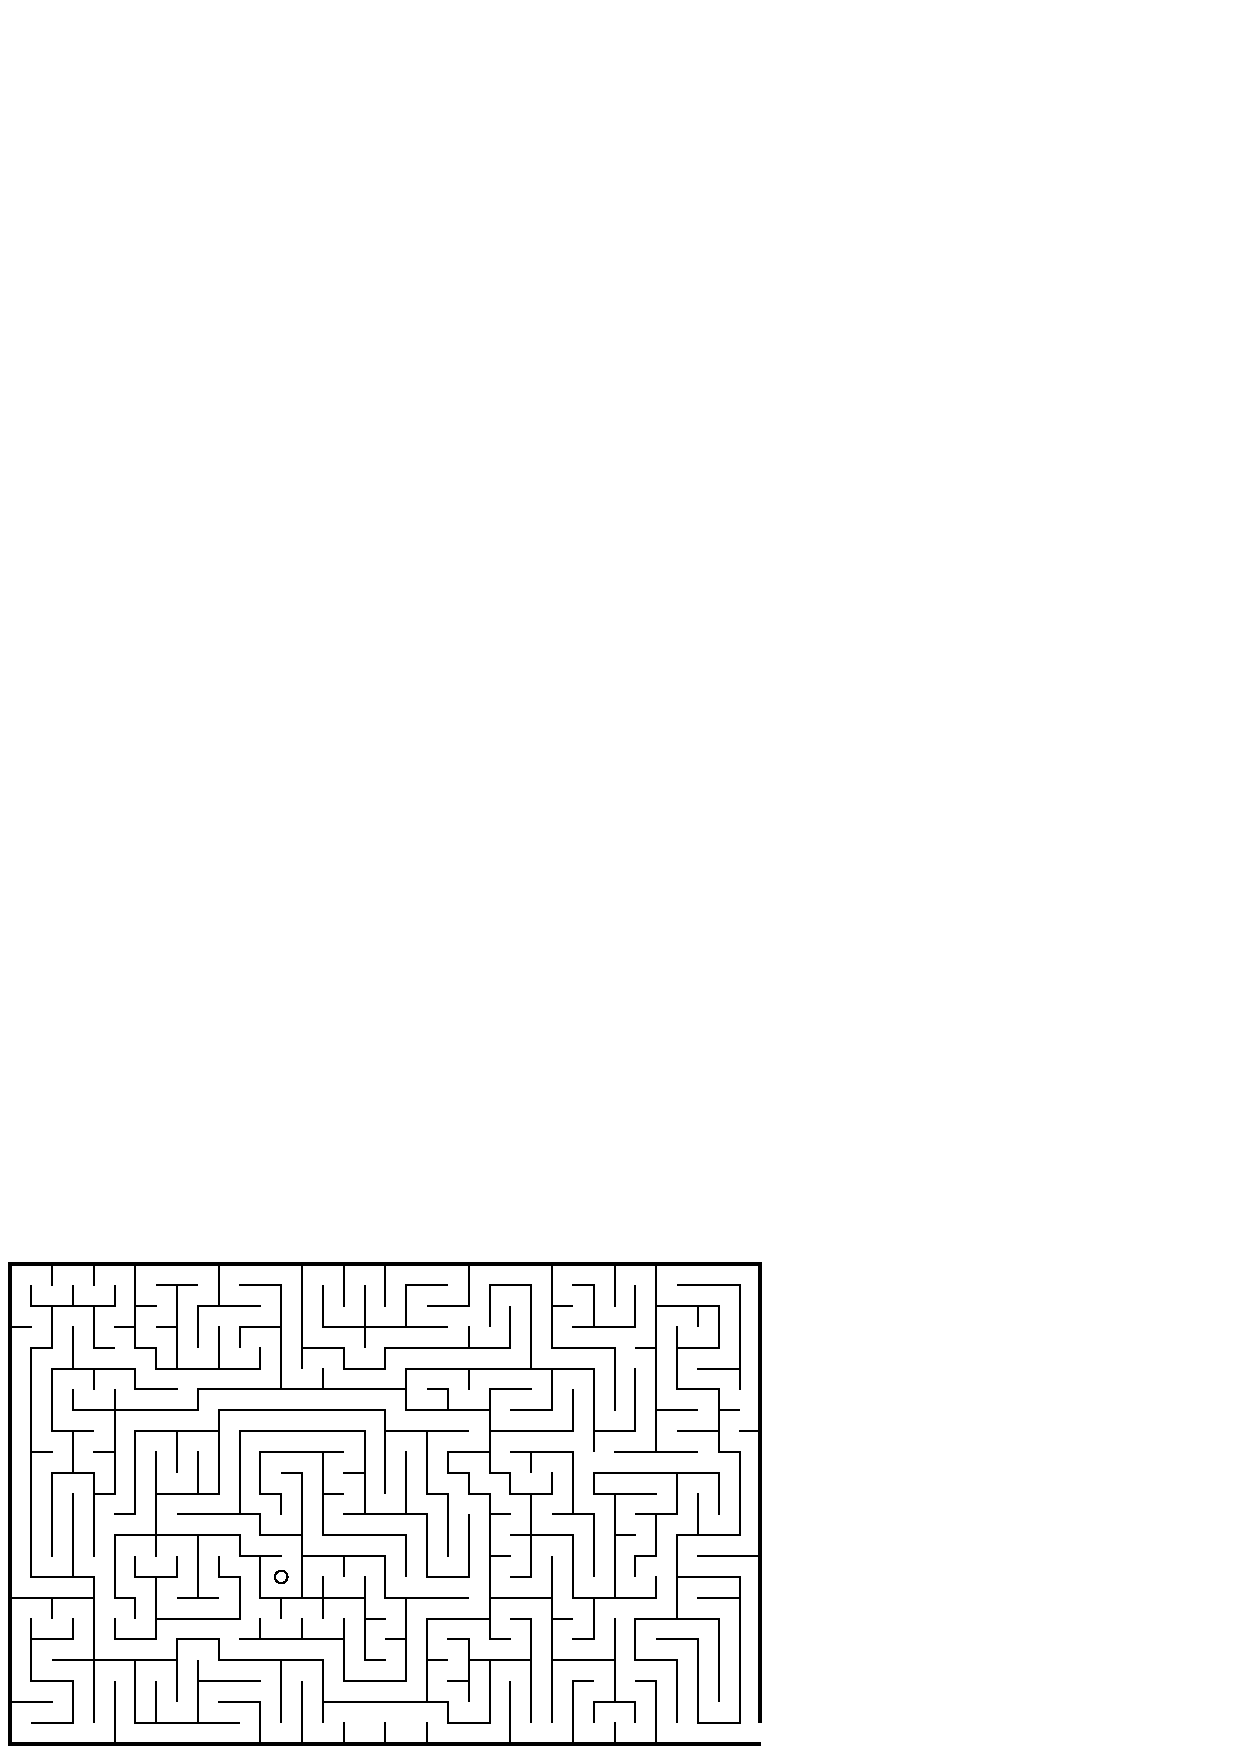
\includegraphics
[height=\ifPaper.6\textwidth\else.7\textheight\fi]{./images/illus197}}
\label{illus:197}
\end{figure*}
in my own garden on a plot of ground which would not allow
of more than $36$ by $23$ paths, but it will be noticed that none
of the nodes are of a high order\index{Labyrinths|)}\index{Mazes|)}.

\section{Geometrical Trees} Euler's original investigations\index
{Trees@\textsc{Trees, Geometrical}|(} were
confined to a closed network. In the problem of the maze it
was assumed that there might be any number of blind alleys
in it, the ends of which formed free nodes. We may now
progress one step farther, and suppose that the network or
closed part of the figure diminishes to a point. This last
arrangement is known as a \emph{tree}. The number of unicursal
descriptions necessary to completely describe a tree is called
the \emph{base} of the ramification\index{Ramification}.

We can illustrate the possible form of these trees by rods,
having a hook at each end. Starting with one such rod, we
can attach at either end one or more similar rods. Again,
on any free hook we can attach one or more similar rods,
and so on. Every free hook, and also every point where two
\PG----File: 198.png------------------------------------------------------
or more rods meet, are what hitherto we have called nodes.
The rods are what hitherto we have termed branches or paths.

The theory of trees---which already plays a somewhat
important part in certain branches of modern analysis, and
possibly may contain the key to certain chemical and biological
theories---originated in a memoir by Cayley\index{Cayley}\footnote
{\textit{Philosophical Magazine}, March, 1857, series~4, vol.~\textsc{xiii},
pp.~172--176; or \textit{Collected Works}, Cambridge, 1890,
vol.~\textsc{iii}, no.~203, pp.~242--346:
see also the paper on double partitions, \textit{Philosophical Magazine},
November, 1860, series~4, vol.~\textsc{xx}, pp.~337--341. On the number of
trees with a given number of nodes, see the \textit
{Quarterly Journal of Mathematics},
London, 1889, vol.~\textsc{xxiii}, pp.~376--378. The connection with
chemistry was first pointed out in Cayley's paper on isomers, \textit
{Philosophical Magazine},
June, 1874, series~4, vol.~\textsc{xlvii}, pp.~444--447, and
was treated more fully in his report on trees to the British Association in
1875, \textit{Reports}, pp.~257--305.}, written in
1856. The discussion of the theory has been analytical rather
than geometrical. I content myself with noting the following results.

The number of trees with $n$ given nodes is $n^{n-2}$. If $A_n$ is
the number of trees with $n$ branches, and $B_n$ the number of
trees with $n$ free branches which are bifurcations at least,
then
\begin{align*}
(1-x)^{-1} (1-x^2)^{-A_1} (1-x^3)^{-A_2} \dotsm
 & = 1 + A_1 x + A_2 x^2 + A_3 x^3 + \dotsb\, ,\\
(1-x)^{-1} (1-x^2)^{-B_2} (1-x^3)^{-B_3} \dotsm
 & = 1 + x + 2B_2 x^2 + 2B_3 x^3 + \dotsb\,.
\end{align*}
Using these formulae we can find successively the values of
$A_1,A_2,\dots$, and $B_1,B_2,\dots$. The values of $A_n$ when $n = 2$, $3$,
$4$, $5$, $6$, $7$, are $2$, $4$, $9$, $20$, $48$, $115$; and of $B_n$ are
$1$, $2$, $5$, $12$,
$33$, $90$\index{Trees@\textsc{Trees, Geometrical}|)}\index{Ramification}.

\ThoughtBreakSpace
I turn next to consider some problems where it is desired
to find a route which will pass once and only once through
each node of a given geometrical figure. This is the reciprocal
of the problem treated in the first part of this chapter, and is
a far more difficult question. I am not aware that the general
theory has been considered by mathematicians, though two
\PG----File: 199.png-----------------------------------------------------
special cases---namely, the \emph{Hamiltonian} (or Icosian) \emph{Game}
and the \emph{Knight's Path on a Chess-Board}---have been treated in
some detail; and I confine myself to a discussion of these.

\section{The Hamiltonian Game} The Hamiltonian Game%
\index{Dodecahedron@\textsc{Dodecahedron Game}|(}%
\index{Hamilton, Sir Wm.|(}%
\index{Hamiltonian@\textsc{Hamiltonian Game}|(}%
\index{Icosian@\textsc{Icosian Game}|(} consists
in the determination of a route along the edges of a regular
dodecahedron which will pass once and only once through
every angular point. Sir William Hamilton\footnote
{See \textit{Quarterly Journal of Mathematics}, London, 1862,
vol.~\textsc{v}, p.~305;
or \textit{Philosophical Magazine}, January, 1884, series~5,
vol.~\textsc{xvii}, p.~42; also
Lucas\index{Lucas, E.}, vol.~\textsc{ii}, part~vii.}, who invented
this game---if game is the right term for it---denoted the
twenty angular points on the solid by letters which stand for
various towns. The thirty edges constitute the only possible
paths. The inconvenience of using a solid is considerable,
and the dodecahedron may be represented conveniently in
perspective by a flat board marked as shown in the first of
the annexed diagrams. The second and third diagrams will
answer our purpose equally well and are easier to draw.

\begin{figure*}[!hbt]
\centerline{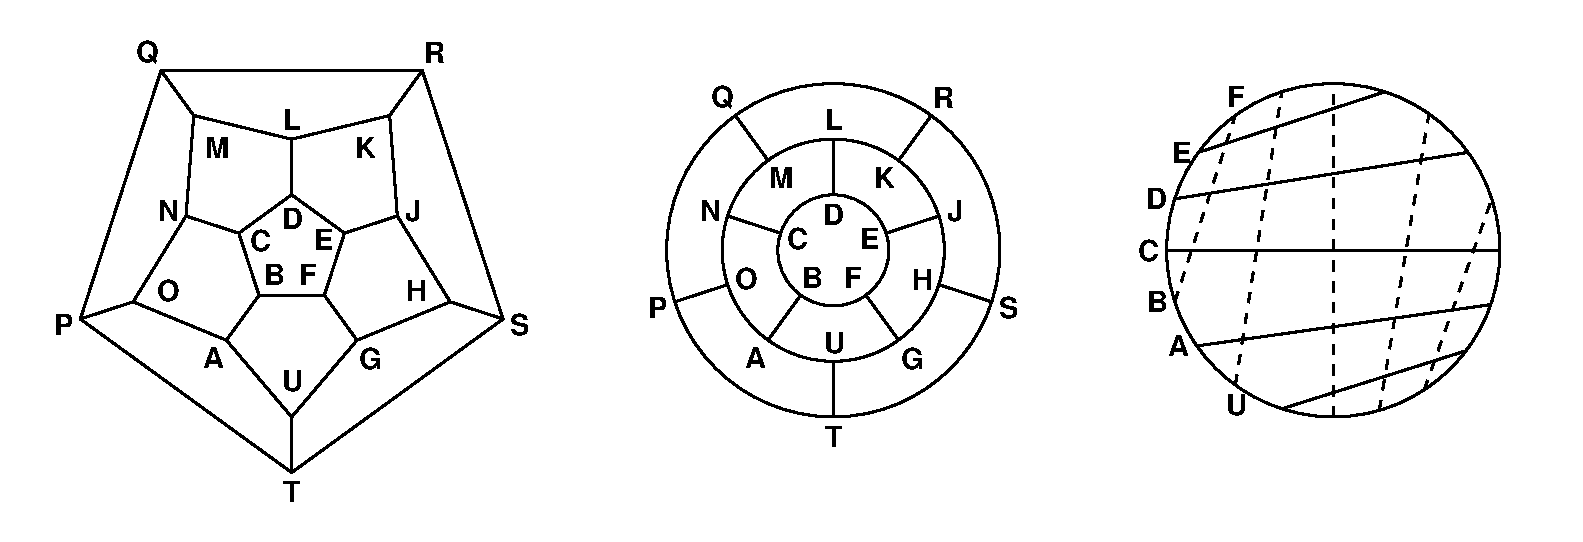
\includegraphics[width=\textwidth]{./images/illus199}}
\label{illus:199}
\end{figure*}

The first problem is go ``all round the world,'' that is,
starting from any town, to go to every other town once and
only once and to return to the initial town; the order of the $n$
towns to be first visited being assigned, where $n$ is not greater
than five.

Hamilton's rule for effecting this was given at the meeting
in 1857 of the British Association at Dublin. At each
angular point there are three and only three edges. Hence,
\PG----File: 200.png-----------------------------------------------------
if we approach a point by one edge, the only routes open to
us are one to the right, denoted by $r$, and one to the left,
denoted by $l$. It will be found that the operations indicated
on opposite sides of the following equalities are equivalent,
\[
lr^2l = rlr,\quad rl^2r = lrl,\quad lr^3l=r^2,\quad rl^3r=l^2\,.
\]
Also the operation $l^5$ or $r^5$ brings us back to the initial point:
we may represent this by the equations
\[
l^5=1,\quad r^5=1\,.
\]

To solve the problem for a figure having twenty angular
points we must deduce a relation involving twenty successive
operations, the total effect of which is equal to unity. By
repeated use of the relation $l^2 = rl^3r$ we see that
\begin{LRalign}
&1=l^5=l^2l^3=(rl^3r)l^3&=\{rl^3\}^2=\{r(rl^3r)l\}^2\\
&&=\{r^2l^3rl\}^2=\{r^2(rl^3r)lrl\}^2=\{r^3l^3rlrl\}^2\,.\\
Therefore && \{r^3l^3(rl)^2\}^2=1&\hbox to2cm{\dotfill(i),}\\
and similarly& & \{l^3r^3(lr)^2\}^2=1&\hbox to2cm{\dotfill(ii).}\\
\end{LRalign}
Hence on a dodecahedron either of the operations
\begin{gather*}
r~r~r~l~l~l~r~l~r~l~r~r~r~l~l~l~r~l~r~l\tag{i}\\
l~l~l~r~r~r~l~r~l~r~l~l~l~r~r~r~l~r~l~r\tag{ii}
\end{gather*}
indicates a route which takes the traveller through every town,
The arrangement is cyclical, and the route can be commenced
at any point in the series of operations by transferring the
proper number of letters from one end to the other. The
point at which we begin is determined by the order of certain
towns which is given initially.

Thus, suppose that we are told that we start from $F$ and
then successively go to $B$, $A$, $U$, and $T$, and we want to find
a route from $T$ through all the remaining towns which will
end at $F$. If we think of ourselves as coming into $F$ from
$G$, the path $FB$ would be indicated by $l$, but if we think of
ourselves as coming into $F$ from $E$, the path $FB$ would be
indicated by $r$. The path from $B$ to $A$ is indicated by $l$,
and so on. Hence our first paths are indicated either by $l\;l\;l\;r$
or by $r\;l\;l\;r$. The latter operation does not occur either in (i)
\PG----File: 201.png-----------------------------------------------------
or in (ii), and therefore does not fall within our solutions. The
former operation may be regarded either as the $1$st, $2$nd, $3$rd,
and $4$th steps of (ii), or as the $4$th, $5$th, $6$th, and $7$th steps
of (i). Each of these leads to a route which satisfies the
problem. These routes are
\begin{LRalign}
&F~B~A~U~T~P~O~N~C~D~E~J~K~L~M~Q~R~S~H~G~F\,,&&\\
and&F~B~A~U~T~S~R~K~L~M~Q~P~O~N~C~D~E~J~H~G~F\,.&&\\
\end{LRalign}

It is convenient to make a mark or to put down a counter
at each corner as soon as it is reached, and this will prevent
our passing through the same town twice.

A similar game may be played with other solids provided
that at each angular point three and only three edges meet. Of
such solids a tetrahedron and a cube are the simplest instances,
but the reader can make for himself any number of plane
figures representing such solids similar to those drawn
\vpageref{illus:199}. % [*Note: originally "on the last page"
Some of these were indicated by Hamilton. In all
such cases we must obtain from the formulae analogous to
those given above cyclical relations like (i) or (ii) there given.
The solution will then follow the lines indicated above. This
method may be used to form a rule for describing any maze in
which no node is of an order higher than three.

For solids having angular points where more than three
edges meet---such as the octahedron where at each angular
point four edges meet, or the icosahedron where at each
angular point five edges meet---we should at each point have
more than two routes open to us; hence (unless we suppress
some of the edges) the symbolical notation would have to be
extended before it could be applied to these solids. I offer
the suggestion to anyone who is desirous of inventing a new
game.

Another and a very elegant solution of the Hamiltonian
dodecahedron problem has been given by M.~Hermary\index{Hermary}. It
consists in unfolding the dodecahedron into its twelve pentagons,
each of which is attached to the preceding one by only
one of its sides; but the solution is geometrical, and not
directly applicable to more complicated solids.

\PG----File: 202.png-----------------------------------------------------
Hamilton suggested as another problem to start from any
town, to go to certain specified towns in an assigned order,
then to go to every other town once and only once, and to end
the journey at some given town. He also suggested the consideration
of the way in which a certain number of towns
should be blocked so that there was no passage through them,
in order to produce certain effects. These problems have not,
so far as I know, been subjected to mathematical analysis%
\index{Dodecahedron@\textsc{Dodecahedron Game}|)}%
\index{Hamilton, Sir Wm.|)}%
\index{Hamiltonian@\textsc{Hamiltonian Game}|)}%
\index{Icosian@\textsc{Icosian Game}|)}.

\section{Knight's Path on a Chess-Board} Another geometrical%
\index{Chess-board, Games@\textsc{Chess-board, Games on}|(}%
\index{Chess-board, knights@\nobreak--- knights' moves on|(}%
\index{Chess-board, problems@\nobreak--- problems|(}%
\index{Knight@\textsc{Knight's Path Problem}|(}%
\index{Routes on a Chess-board}
problem on which a great deal of ingenuity has been expended,
and of a kind somewhat similar to the Hamiltonian game,
consists in moving a knight on a chess-board in such a manner
that it shall move successively on to every cell\footnote
{The $64$ small squares into which a chess-board is divided are termed
\emph{cells}\index{Cells of a Chess-board}.} once and only
once. The literature on this subject is so extensive\footnote
{For a bibliography see A.~van der Linde\index{Linde on Knight's Path},
\textit{Geschichte und Literatur
des Schachspiels}, Berlin, 1874, vol.~\textsc{ii}, pp.~101--111.
On the problem
see a memoir by P.~Volpicelli\index{Volpicelli on Knight's Path}
in \textit{Atti della Reale Accademia dei Lincei},
Rome, 1872, vol.~\textsc{xxv}, pp.~87--162: also \textit
{Applications de l'Analyse
Mathématique au Jeu des échecs}, by C.F.~de~Jaenisch\index
{Jaenisch}, 3~vols., St~Petersburg,
1862--3; and General Parmentier\index{Parmentier on Knight's Path},
\textit{Association Française pour
l'avancement des Sciences}, 1891, 1892, 1894.} that I
make no pretence to give a full account of the various methods
for solving the problem, and I shall content myself by putting
together a few notes on some of the solutions I have come
across, particularly on those due to De~Moivre, Euler, Vandermonde\index
{Vandermonde}, Warnsdorff, and Roget.

On a board containing an even number of cells the path
may or may not be re-entrant, but on a board containing an
odd number of cells it cannot be re-entrant. For, if a knight
begins on a white cell, its first move must take it to a black
cell, the next to a white cell, and so on. Hence, if its path
passes through all the cells, then on a board of an odd number
of cells the last move must leave it on a cell of the same colour
\PG----File: 203.png-----------------------------------------------------
as that on which it started, and therefore these cells cannot be
connected by one move.

\phantomsection
\addcontentsline{toc}{subsection}{Method of De Montmort and De Moivre}
The earliest solutions of which I have any knowledge are
those given about the end of the seventeenth century by
De~Montmort\index{DeMontmort@De Montmort}\index{Montmort, De} and
De~Moivre\index{DeMoivre@De Moivre, on Knight's Move}\index
{Moivre, A. De}\footnote
{I do not know where they were published originally; they were
quoted by Ozanam\index{Ozanam@Ozanam's \textit{Récréations}}
and Montucla\index{Montucla}, see Ozanam, 1803 edition, vol.~\textsc{i},
p.~178; 1840 edition, p.~80.}. They apply to the ordinary
chess-board of $64$ cells, and depend on dividing (mentally) the
board into an inner square containing sixteen cells surrounded
by an outer ring of cells two deep. If initially the knight is
placed on a cell in the outer ring, it moves round that ring
always in the same direction so as to fill it up completely---only
going into the inner square when absolutely necessary.
When the outer ring is filled up the order of the moves
required for filling the remaining cells presents but little difficulty.
If initially the knight is placed on the inner square
the process must be reversed. The method can be applied to
square and rectangular boards of all sizes. It is illustrated
sufficiently by De Moivre's solution which is given
\vpageref[below]{DeMoivre},
\begin{figure*}[!hbt]
\centering
\hspace*{\fill}
\begin{minipage}[b]{.4\textwidth}
\centering
\begin{MagicSquare}{8}
{34} & {49} & {22} & {11} & {36} & {39} & {24} & 1 \\
{21} & {10} & {35} & {50} & {23} & {12} & {37} & {40} \\
{48} & {33} & {62} & {57} & {38} & {25} & 2 & {13} \\
9 & {20} & {51} & {54} & {63} & {60} & {41} & {26} \\
{32} & {47} & {58} & {61} & {56} & {53} & {14} & 3 \\
{19} & 8 & {55} & {52} & {59} & {64} & {27} & {42} \\
{46} & {31} & 6 & {17} & {44} & {29} & 4 & {15} \\
7 & {18} & {45} & {30} & 5 & {16} & {43} & {28}
\end{MagicSquare}
\legend{De Moivre's Solution.}
\end{minipage}
\hfill
\begin{minipage}[b]{.4\textwidth}
\centering
\begin{MagicSquare}{6}
{30} & {21} & 6 & {15} & {28} & {19} \\
7 & {16} & {29} & {20} & 5 & {14} \\
{22} & {31} & 8 & {35} & {18} & {27} \\
9 & {36} & {17} & {26} & {13} & 4 \\
{32} & {23} & 2 & {11} & {34} & {25} \\
1 & {10} & {33} & {24} & 3 & {12}
\end{MagicSquare}
\legend{Euler's Thirty-six Cell Solution.}
\end{minipage}
\hspace*{\fill}
\label{DeMoivre}
\end{figure*}
where the numbers indicate the order in which the cells
are occupied successively. I place by its side a somewhat
similar re-entrant solution, due to Euler\index{Euler}, for a board of
\PG----File: 204.png-----------------------------------------------------
$36$ cells. If a chess-board is used it is convenient to place
a counter on each cell as the knight leaves it.

\phantomsection
\addcontentsline{toc}{subsection}{Method of Euler}
The next serious attempt to deal with the subject was
made by Euler\index{Euler|(}\footnote
{\textit{Mémoires de Berlin} for 1759, Berlin, 1766, pp.~310--337; or
\textit{Commentationes
Arithmeticae Collectae}, St~Petersburg, 1849, vol.~\textsc{i}, pp.~337--355.}
in 1759: it was due to a suggestion made by
L.~Bertrand\index{Bertrand,~L. (of Geneva)} of Geneva, who subsequently
(in 1778) issued an
account of it. This method is applicable to boards of any
shape and size, but in general the solutions to which it
leads are not symmetrical and their mutual connexion is not
apparent.

Euler commenced by moving the knight at random over
the board until it has no move open to it. With care this
will leave only a few cells not traversed: denote them by
$a, b, \dots$. His method consists in establishing certain rules by
which these vacant cells can be interpolated into various parts
of the circuit, and also by which the circuit can be made
re-entrant.

The following example, mentioned by Legendre\index{Legendre} as one of
exceptional difficulty, illustrates the method. Suppose that we
\begin{figure*}[!hbt]
\centering
\ifPaper\else\hspace*{\fill}\fi
\begin{minipage}{.4\textwidth}
\centering
\begin{MagicSquare}{8}
{55} & {58} & {29} & {40} & {27} & {44} & {19} & {22} \\
{60} & {39} & {56} & {43} & {30} & {21} & {26} & {45} \\
{57} & {54} & {59} & {28} & {41} & {18} & {23} & {20} \\
{38} & {51} & {42} & {31} & 8 & {25} & {46} & {17} \\
{53} & {32} & {37} & {a} & {47} & {16} & 9 & {24} \\
{50} & 3 & {52} & {33} & {36} & 7 & {12} & {15} \\
1 & {34} & 5 & {48} & {b} & {14} & {c} & {10} \\
4 & {49} & 2 & {35} & 6 & {11} & {d} & {13}
\end{MagicSquare}
\legend{Figure \Uproman{1}}
\end{minipage}
\hfill
\begin{minipage}{.4\textwidth}
\centering
\begin{MagicSquare}{8}
{22} & {25} & {50} & {39} & {52} & {35} & {60} & {57} \\
{27} & {40} & {23} & {36} & {49} & {58} & {53} & {34} \\
{24} & {21} & {26} & {51} & {38} & {61} & {56} & {59} \\
{41} & {28} & {37} & {48} & 3 & {54} & {33} & {62} \\
{20} & {47} & {42} & {13} & {32} & {63} & 4 & {55} \\
{29} & {16} & {19} & {46} & {43} & 2 & 7 & {10} \\
{18} & {45} & {14} & {31} & {12} & 9 & {64} & 5 \\
{15} & {30} & {17} & {44} & 1 & 6 & {11} & 8
\end{MagicSquare}
\legend{Figure \Uproman{2}}
\end{minipage}
\ifPaper\else\hspace*{\fill}\fi
\legend{Example of Euler's Method.}
\DPlabel{Euler:i}
\end{figure*}
have formed the route given in \vhyperlink{Euler:i}{figure~i}; namely, $1$,
%[*Note: originally "figure i above", but in screen the diagram came out below
% and \vpageref got stuck in a pagebreak loop :-(]
$2$, $3$, $\dots$, $59$, $60$; and that there are four cells left
untraversed, namely, $a$, $b$, $c$, $d$.

We begin by making the path $1$ to $60$ re-entrant. The
\PG----File: 205.png-----------------------------------------------------
cell $1$ commands a cell $p$, where $p$ is $32$, $52$, or $2$. The cell $60$
commands a cell $q$, where $q$ is $29$, $59$, or $51$. Then, if any of
these values of $p$ and $q$ differ by unity, we can make the route
re-entrant. This is the case here if $p=52$, $q=51$. Thus the
cells $1, 2, 3, \dotsc, 51$; $60, 59, \dotsc, 52$ form a re-entrant route of
$60$ moves. Hence, if we replace the numbers $60, 59, \dotsc, 52$ by
$52, 53, \dotsc, 60$, the steps will be numbered consecutively. I
recommend the reader who wishes to follow the subsequent
details of Euler's argument to construct this square on a piece
of paper before proceeding further.

Next, we add the cells $a$, $b$, $d$ to this route. In the new
diagram of $60$ cells formed as above the cell $a$ commands the
cells there numbered $51$, $53$, $41$, $25$, $7$, $5$, and $3$. It is
indifferent which of these we select: suppose we take $51$. Then
we must make $51$ the last cell of the route of $60$ cells, so that
we can continue with $a$, $b$, $d$. Hence, if the reader will add $9$
to every number on the diagram he has constructed, and then
replace $61, 62, \dotsc, 69$ by $1, 2, \dotsc, 9$, he will have a route which
starts from the cell occupied originally by $60$, the $60$th move
is on to the cell occupied originally by $51$, and the $61$st, $62$nd,
$63$rd moves will be on the cells $a$, $b$, $d$ respectively.

It remains to introduce the cell $c$. Since $c$ commands the
cell now numbered $25$, and $63$ commands the cell now numbered
$24$, this can be effected in the same way as the first
route was made re-entrant. In fact the cells numbered $1,
2, \dotsc, 24$; $63, 62, \dotsc, 25, c$ form a knight's path. Hence we
must replace $63, 62, \dotsc, 25$ by the numbers $25, 26, \dotsc, 63$, and
then we can fill up $c$ with $64$. We have now a route which
covers the whole board.

Lastly, it remains to make this route re-entrant. First, we
must get the cells $1$ and $64$ near one another. This can be
effected thus. Take one of the cells commanded by $1$, such as
$28$, then $28$ commands $1$ and $27$. Hence the cells $64, 63, \dotsc, 28$;
$1, 2, \dotsc, 27$ form a route; and this will be represented in the
diagram if we replace the cells numbered $1, 2, \dotsc, 27$ by $27,
26, \dotsc, 1$.

\PG----File: 206.png--------------------------------------------------
The cell now occupied by $1$ commands the cells $26$, $38$, $54$,
$12$, $14$, $16$, $28$; and the cell occupied by $64$ commands the
cells $13$, $43$, $63$, $55$. The cells $13$ and $14$ are consecutive, and
therefore the cells $64, 63, \dotsc, 14$; $1, 2, \dotsc, 13$ form a route.
Hence we must replace the numbers $1, 2, \dotsc, 13$ by $13, 12, \dotsc, 1$,
and we obtain a re-entrant route covering the whole board,
which is represented in the second of the diagrams given
\vpageref{Euler:i}. %[*Note: originally "above"]
Euler showed how seven other re-entrant routes can
be deduced from any given re-entrant route.

It is not difficult to apply the method so as to form a route
which begins on one given cell and ends on any other given
cell.

Euler next investigated how his method could be modified
so as to allow of the imposition of additional restrictions.

An interesting example of this kind is where the first $32$
moves are confined to one half of the board. One solution
of this is delineated \vpageref[below]{figure:Roget}.
The order of the first $32$ moves
\begin{figure*}[!hbt]
\centering
\ifPaper\else\hspace*{\fill}\fi
\begin{minipage}{.4\textwidth}
\centering
\begin{MagicSquare}{8}
{58} & {43} & {60} & {37} & {52} & {41} & {62} & {35} \\
{49} & {46} & {57} & {42} & {61} & {36} & {53} & {40} \\
{44} & {59} & {48} & {51} & {38} & {55} & {34} & {63} \\
{47} & {50} & {45} & {56} & {33} & {64} & {39} & {54} \\
{22} &  7 & {32} &  1 & {24} & {13} & {18} & {15} \\
{31} &  2 & {23} &  6 & {19} & {16} & {27} & {12} \\
 8 & {21} &  4 & {29} & {10} & {25} & {14} & {17} \\
 3 & {30} &  9 & {20} &  5 & {28} & {11} & {26}\\
\put(0,4){\line(1,0){8}}
\end{MagicSquare}
\legend{Euler's Half-board Solution.}
\end{minipage}
\hfill
\begin{minipage}{.4\textwidth}
\centering
\begin{MagicSquare}{8}
{50} & {45} & {62} & {41} & {60} & {39} & {54} & {35} \\
{63} & {42} & {51} & {48} & {53} & {36} & {57} & {38} \\
{46} & {49} & {44} & {61} & {40} & {59} & {34} & {55} \\
{43} & {64} & {47} & {52} & {33} & {56} & {37} & {58} \\
{26} &  5 & {24} &  1 & {20} & {15} & {32} & {11} \\
{23} &  2 & {27} &  8 & {29} & {12} & {17} & {14} \\
 6 & {25} &  4 & {21} & {16} & {19} & {10} & {31} \\
 3 & {22} &  7 & {28} &  9 & {30} & {13} & {18}\\
\put(0,4){\line(1,0){8}}
\end{MagicSquare}
\legend{Roget's Half-board Solution.}
\end{minipage}
\ifPaper\else\hspace*{\fill}\fi
\label{figure:Roget}
\end{figure*}
can be determined by Euler's method. It is obvious that, if
to the number of each such move we add $32$, we shall have
a corresponding set of moves from $33$ to $64$ which would cover
the other half of the board; but in general the cell numbered
$33$ will not be a knight's move from that numbered $32$,
nor will $64$ be a knight's move from $1$.

\PG----File: 207.png-----------------------------------------------------
Euler however proceeded to show how the first $32$ moves
might be determined so that, if the half of the board containing
the corresponding moves from $33$ to $64$ was twisted
through two right angles, the two routes would become
united and re-entrant. If $x$ and $y$ are the numbers of a
cell reckoned from two consecutive sides of the board, we
may call the cell whose distances are respectively $x$ and $y$
from the opposite sides a complementary cell. Thus the cells
$(x, y)$ and $(9-x, 9-y)$ are complementary, where $x$ and $y$
denote respectively the column and row occupied by the cell.
Then in Euler's solution the numbers in complementary cells
differ by $32$: for instance, the cell $(3, 7)$ is complementary to
the cell $(6, 2)$, the one is occupied by $57$, the other by $25$.

Roget's method\index{Roget, P.M.}, which is described later, can be also
applied to give half-board solutions. The result is indicated
\vpageref{figure:Roget}. % [*Note: originally "above"]
The close of Euler's memoir is devoted to showing how
the method could be applied to crosses and other rectangular
figures. I may note in particular his elegant re-entrant symmetrical
solution for a square of $100$ cells\index{Euler|)}.

\phantomsection
\addcontentsline{toc}{subsection}{Method of Vandermonde}
The next attempt of any special interest is due to Vandermonde\index
{Vandermonde}\footnote
{\textit{L'Histoire de l'Académie des Sciences} for 1771, Paris,
1774, pp. 566-574.},
who reduced the problem to arithmetic. His idea was
to cover the board by two or more independent routes taken at
random, and then to connect the routes. He defined the position
of a cell by a fraction $x/y$, whose numerator $x$ is the
number of the cell from one side of the board, and whose denominator
$y$ is its number from the adjacent side of the board;
this is equivalent to saying that $x$ and $y$ are the co-ordinates of
a cell. In a series of fractions denoting a knight's path, the
differences between the numerators of two consecutive fractions
can be only one or two, while the corresponding difference
between their denominators must be two or one respectively.
Also $x$ and $y$ cannot be less than $1$ or greater than $8$. The
notation is convenient, but Vandermonde applied it merely
to obtain a particular solution of the problem for a board of
\PG----File: 208.png----------------------------------------------------
$64$ cells: the method by which he effected this is analogous to
that established by Euler, but it is applicable only to squares
of an even order. The route that he arrives at is defined in
his notation by the following fractions.

\noindent{\baselineskip=1.5\baselineskip
$\frac{5}{5}$, $\frac{4}{3}$, $\frac{2}{4}$, $\frac{4}{5}$, $\frac{5}{3}$,
$\frac{7}{4}$, $\frac{8}{2}$, $\frac{6}{1}$,
$\frac{7}{3}$, $\frac{8}{1}$, $\frac{6}{2}$,
$\frac{8}{3}$, $\frac{7}{1}$, $\frac{5}{2}$,
$\frac{6}{4}$, $\frac{8}{5}$, $\frac{7}{7}$,
$\frac{5}{8}$, $\frac{6}{6}$, $\frac{5}{4}$,
$\frac{4}{6}$, $\frac{2}{5}$, $\frac{1}{7}$,
$\frac{3}{8}$,
$\frac{2}{6}$, $\frac{1}{8}$, $\frac{3}{7}$, $\frac{1}{6}$, $\frac{2}{8}$,
$\frac{4}{7}$, $\frac{3}{5}$, $\frac{1}{4}$,
$\frac{2}{2}$, $\frac{4}{1}$, $\frac{3}{3}$,
$\frac{1}{2}$, $\frac{3}{1}$, $\frac{2}{3}$,
$\frac{1}{1}$, $\frac{3}{2}$, $\frac{1}{3}$,
$\frac{2}{1}$, $\frac{4}{2}$, $\frac{3}{4}$,
$\frac{1}{5}$, $\frac{2}{7}$, $\frac{4}{8}$,
$\frac{3}{6}$,
$\frac{4}{4}$, $\frac{5}{6}$, $\frac{7}{5}$, $\frac{8}{7}$, $\frac{6}{8}$,
$\frac{7}{6}$, $\frac{8}{8}$, $\frac{6}{7}$,
$\frac{8}{6}$, $\frac{7}{8}$, $\frac{5}{7}$,
$\frac{6}{5}$, $\frac{8}{4}$, $\frac{7}{2}$,
$\frac{5}{1}$, $\frac{6}{3}$.

}\medskip
The path is re-entrant but unsymmetrical. Had he transferred
the first three fractions to the end of this series he
would have obtained two symmetrical circuits of thirty-two
moves joined unsymmetrically, and might have been enabled
to advance further in the problem. Vandermonde\index{Vandermonde}
also considered the case of a route in a cube.

In 1773 Collini\index{Collini on Chess}\footnote
{\textit{Solution du Problème du Cavalier au Jeu des échecs}, Mannheim,
1773.} proposed the exclusive use of symmetrical
routes arranged without reference to the initial cell, but connected
in such a manner as to permit of our starting from
it. This is the foundation of the modern manner of attacking
the problem. The method was re-invented in 1825 by
Pratt\index{Pratt on Knight's Path}\footnote
{\textit{Studies of Chess}, sixth edition, London, 1825.},
and in 1840 by Roget\index{Roget, P.M.}, and has been subsequently
employed by various writers. Neither Collini nor Pratt showed
skill in using this method. The rule given by Roget is described
later.

\phantomsection
\addcontentsline{toc}{subsection}{Method of Warnsdorff}
One of the most ingenious of the solutions of the knight's
path is that given in 1823 by Warnsdorff\index
{Warnsdorff, Knight's Path|(}\footnote
{\textit{Des Rösselsprunges einfachste und allgemeinste Lösung},
Schmalkalden, 1823: see Jaenisch\index{Jaenisch},
vol.~\textsc{ii}, pp.~56--61, 273--289.}. His rule is that
the knight must be moved always to one of the cells from
which it will command the fewest squares not already traversed.
The solution is not symmetrical and not re-entrant;
moreover it is difficult to trace practically. The rule has not
been proved to be true, but no exception to it is known:
apparently it applies also to all rectangular boards which can
\PG----File: 209.png-----------------------------------------------------
be covered completely by a knight. It is somewhat curious
that in most cases a single false step, except in the last three
or four moves, will not affect the result.

Warnsdorff added that when, by the rule, two or more cells
are open to the knight, it may be moved to either or any of
them indifferently. This is not so, and with great ingenuity
two or three cases of failure have been constructed, but it
would require exceptionally bad luck to happen accidentally
on such a route\index{Warnsdorff, Knight's Path|)}.

The above methods have been applied to boards of various
shapes, especially to boards in the form of rectangles, crosses,
and circles\footnote
{See \Eg\ T.~Ciccolini's\index{Ciccolini on Chess} work \textit
{Del Cavallo degli Scacchi}, Paris, 1836.}.

All the more recent investigations impose additional restrictions:
such as to require that the route shall be re-entrant, or
more generally that it shall begin and terminate on given
cells.

\phantomsection
\addcontentsline{toc}{subsection}{Method of Roget}
The best complete solution with which I am acquainted---and
one which I believe is not generally known---is due to
Roget\index{Roget, P.M.|(}\footnote
{\textit{Philosophical Magazine}, April, 1840, series~3, vol.~\textsc{xvi},
pp.~305--309; see also the \textit{Quarterly Journal of Mathematics} for 1877,
vol.~\textsc{xiv}, pp.~354--359. Some solutions, founded on Roget's method,
are given in the \textit{Leisure Hour}, Sept.~13, 1873, pp. 587--590;
see also \Ibid, Dec.~20, 1873, pp.~813--815.
}. It divides the whole route into four circuits, which
can be combined so as to enable us to begin on any cell
and terminate on any other cell of a different colour. Hence,
if we like to select this last cell at a knight's move from the
initial cell, we obtain a re-entrant route. On the other hand,
the rule is applicable only to square boards containing $(4n)^2$
cells: for example, it could not be used on the board of the
French \emph{jeu des dames}, which contains $100$ cells.

Roget began by dividing the board of $64$ cells into four
quarters. Each quarter contains $16$ cells, and these $16$ cells
can be arranged in $4$ groups, each group consisting of $4$ cells
\PG----File: 210.png-------------------------------------------------------
which form a closed knight's path. All the cells in each such
path are denoted by the same letter $l$, $e$, $a$, or $p$, as the case
nay be. The path of $4$ cells indicated by the consonants $l$ and
the path indicated by the consonants $p$ are diamond-shaped:
the paths indicated respectively by the vowels $e$ and $a$ are
square-shaped, as may be seen by looking at one of the four
quarters in figure~i \vpageref[below]{Roget:i}.

\begin{figure*}[!hbt]
\centering
\ifPaper\else\hspace*{\fill}\fi
\begin{minipage}{.4\textwidth}
\centering
\def\SqHtDefault{lp}
\begin{MagicSquare}{8}
l & e & a & p & l & e & a & p \\
a & p & l & e & a & p & l & e \\
e & l & p & a & e & l & p & a \\
p & a & e & l & p & a & e & l \\
l & e & a & p & l & e & a & p \\
a & p & l & e & a & p & l & e \\
e & l & p & a & e & l & p & a \\
p & a & e & l & p & a & e & l \\
\put(0,4){\line(1,0){8}}
\put(4,0){\line(0,1){8}}
\end{MagicSquare}
\legend{Roget's Solution \upshape(i).}
\end{minipage}
\hfill
\begin{minipage}{.4\textwidth}
\centering
\begin{MagicSquare}{8}
{34} & {51} & {32} & {15} & {38} & {53} & {18} & 3 \\
{31} & {14} & {35} & {52} & {17} & 2 & {39} & {54} \\
{50} & {33} & {16} & {29} & {56} & {37} & 4 & {19} \\
{13} & {30} & {49} & {36} & 1 & {20} & {55} & {40} \\
{48} & {63} & {28} & 9 & {44} & {57} & {22} & 5 \\
{27} & {12} & {45} & {64} & {21} & 8 & {41} & {58} \\
{62} & {47} & {10} & {25} & {60} & {43} & 6 & {23} \\
{11} & {26} & {61} & {46} & 7 & {24} & {59} & {42}\\
\put(0,4){\line(1,0){8}}
\put(4,0){\line(0,1){8}}
\end{MagicSquare}
\legend{Roget's Solution \upshape(ii).}
\end{minipage}
\ifPaper\else\hspace*{\fill}\fi
\label{Roget:i}
\end{figure*}

Now all the $16$ cells on a complete chess-board which are
marked with the same letter can be combined into one circuit,
and wherever the circuit begins we can make it end on any
other cell in the circuit, provided it is of a different colour
to the initial cell. If it is indifferent on what cell the
circuit terminates we may make the circuit re-entrant, and
in this case we can make the direction of motion round each
group (of $4$ cells) the same.  For example, all the cells
marked $p$ can be arranged in the circuit indicated by the
successive numbers $1$ to $16$ in figure~ii \vpageref[above]{Roget:i}.
Similarly all
the cells marked $a$ can be combined into the circuit indicated
by the numbers $17$ to $23$; all the $l$ cells into the circuit $33$ to
$48$; and all the $e$ cells into the circuit $49$ to $64$. Each of the
circuits indicated above is symmetrical and re-entrant. The
consonant and the vowel circuits are said to be of opposite
kinds.

\PG----File: 211.png-------------------------------------------------------
The general problem will be solved if we can combine the
four circuits into a route which will start from any given cell,
and terminate on the $64$th move on any other given cell of a
different colour. To effect this Roget gave the two following
rules.

First.\quad If the initial cell and the final cell are denoted the
one by a consonant and the other by a vowel, take alternately
circuits indicated by consonants and vowels, beginning with
the circuit of $16$ cells indicated by the letter of the initial
cell and concluding with the circuit indicated by the letter of
the final cell.

Second.\quad If the initial cell and the final cell are denoted
both by consonants or both by vowels, first select a cell, $Y$, in
the same circuit as the final cell, $Z$, and one move from it,
next select a cell, $X$, belonging to one of the opposite circuits
and one move from $Y$. This is always possible. Then, leaving
out the cells $Z$ and $Y$, it always will be possible, by the rule
already given, to travel from the initial cell to the cell $X$ in
$62$ moves, and thence to move to the final cell on the $64$th
move.

In both cases however it must be noticed that the cells in
each of the first three circuits will have to be taken in such an
order that the circuit does not terminate on a corner, and it
may be desirable also that it should not terminate on any of
the border cells. This will necessitate some caution. As far
as is consistent with these restrictions it is convenient to
make these circuits re-entrant, and to take them and every
group in them in the same direction of rotation.

As an example, suppose that we are to begin on the cell
numbered $1$ in figure~ii \vpageref{Roget:i}, which is one of those in a
$p$ circuit, and to terminate on the cell numbered $64$, which is
one of those in an $e$ circuit. This falls under the first rule:
hence first we take the $16$ cells marked $p$, next the $16$ cells
marked $a$, then the $16$ cells marked $l$, and lastly the $16$ cells
marked $e$. One way of effecting this is shown in the diagram.
Since the cell $64$ is a knight's move from the initial cell the
\PG----File: 212.png-------------------------------------------------------
route is re-entrant. Also each of the four circuits in the
diagram is symmetrical, re-entrant, and taken in the same
direction, and the only point where there is any apparent
breach in the uniformity of the movement is in the passage
from the cell numbered $32$ to that numbered $33$.

A rule for re-entrant routes, similar to that of Roget, has
been given by various subsequent writers, especially by
De~Polignac\index{DePolignac@De Polignac on Knight's Move}\index
{Polignac on Knight's Path}\footnote
{\textit{Comptes Rendus}, April, 1861; and \textit{Bulletin de la
Société Mathématique de France}, 1881, vol.~\textsc{ix}, pp. 17--24.}
and by Laquière\index{Laquiere@Laquière on Knight's Path}\footnote
{\textit{Bulletin de la Société Mathématique de France}, 1880,
vol.~\textsc{viii}, pp.~82--102, 132--158.}, who have stated it at much
greater length. Neither of these authors seems to have been
aware of Roget's theorems. De~Polignac, like Roget, illustrates
the rule by assigning letters to the various squares in
the way explained above, and asserts that a similar rule is
applicable to all even squares.

Roget's method can be also applied to two half-boards, as
indicated in the figure given above on page~\pageref{figure:Roget}\index
{Roget, P.M.|)}.

\phantomsection
\addcontentsline{toc}{subsection}{Method of Moon}
Another way of dividing the board into closed circuits
which can be connected was given in $1843$ by Moon\index{Moon, R.}\footnote
{\textit{Cambridge Mathematical Journal}, 1843, vol.~\textsc{iii},
pp.~233--236.}. He
\begin{figure*}[!hbt]
\centering
\ifPaper\else\hspace*{\fill}\fi
\begin{minipage}{.4\textwidth}
\centering
\begin{MagicSquare}{8}
a & b & c & d & a & b & c & d \\
c & d & a & b & c & d & a & b \\
b & a & A & B & C & D & d & c \\
d & c & C & D & A & B & b & a \\
a & b & B & A & D & C & c & d \\
c & d & D & C & B & A & a & b \\
b & a & d & c & b & a & d & c \\
d & c & b & a & d & c & b & a \\
\put(2,2){\line(1,0){4}}
\put(2,2){\line(0,1){4}}
\put(2,6){\line(1,0){4}}
\put(6,2){\line(0,1){4}}
\end{MagicSquare}
\legend{Moon's Solution.}
\end{minipage}
\hfill
\begin{minipage}{.4\textwidth}
\centering
\begin{MagicSquare}{8}
{63} & {22} & {15} & {40} &  1 & {42} & {59} & {18} \\
{14} & {39} & {64} & {21} & {60} & {17} &  2 & {43} \\
{37} & {62} & {23} & {16} & {41} &  4 & {19} & {58} \\
{24} & {13} & {38} & {61} & {20} & {57} & {44} &  3 \\
{11} & {36} & {25} & {52} & {29} & {46} &  5 & {56} \\
{26} & {51} & {12} & {33} &  8 & {55} & {30} & {45} \\
{35} & {10} & {49} & {28} & {53} & {32} & {47} &  6 \\
{50} & {27} & {34} &  9 & {48} &  7 & {54} & {31}
\end{MagicSquare}
\legend{Jaenisch's Solution\index{Jaenisch}.}
\end{minipage}
\ifPaper\else\hspace*{\fill}\fi
\label{Jaenisch}
\end{figure*}
divided the board into a central square containing $4^2$ cells and
a surrounding annulus (see figure \vpageref{Jaenisch}). The annulus may be
\PG----File: 213.png------------------------------------------------------
divided into four closed circuits, each containing $12$ cells: these
are marked respectively with the letters $a$, $b$, $c$, $d$. The central
square may be divided similarly into four closed circuits, each
containing $4$ cells, denoted by the letters $A$, $B$, $C$, $D$. We can
connect these routes as follows. If we are moving outwards
from the central square to the annulus we can go from a cell $A$
either to $b$ or to $c$ or to $d$ (but not to $a$) and similarly for the
other letters. If we are moving inwards from the annulus to
the central square we must go from $a$ to $D$, or $d$ to $A$, or $b$ to
$C$, or $c$ to $B$, as the case may be. Thus if the initial cell is
on $a$, we might take either of the cycles
$a\ D\ b\ C\ d\ A\ c\ B$, or
$a\ D\ c\ B\ d\ A\ b\ C$. By following these rules we always can
connect the routes into one path, but in general it will not
be re-entrant. It is convenient to take the cells in each circuit
in one and the same direction, but a circuit in the outer annulus
must not end in a corner cell, and to avoid this we may
have to alter the direction in which a circuit is taken.

Moon's\index{Moon, R.} rule can be modified to cover the case of any doubly
even square board, and the path can be made to begin and end
on any two given squares, but I do not propose to go further
into details.

\phantomsection
\addcontentsline{toc}{subsection}{Method of Jaenisch}
The method which Jaenisch\index{Jaenisch} gives as the most fundamental
is not very different from that of Roget. It leads to eight
forms, similar to that in the diagram printed \vpageref{Jaenisch}, in which
the sum of the numbers in every column and every row
is $260$; but although symmetrical it is not in my opinion so
easy to reproduce as that given by Roget.

\phantomsection
\addcontentsline{toc}{subsection}{Number of possible routes}
It is as yet impossible to say how many solutions of
the problem exist. Legendre\index{Legendre}\footnote
{\textit{Théorie des Nombres}, Paris, 2nd edition, 1830, vol.~\textsc{ii},
p.~165.} mentioned the question, but
Minding\index{Minding on Knight's Path}\footnote
{\textit{Cambridge and Dublin Mathematical Journal}, 1852, vol.~\textsc{vii},
pp.~147--156; and \textit{Crelle's Journal}, 1853, vol.~\textsc{xliv},
pp.~73--82.} was the earliest writer to attempt to answer it.
More recent investigations have shown that on the one hand
the number of possible routes is less\footnote
{Jaenisch\index{Jaenisch}, vol.~\textsc{ii}, p.~268.} than the number of
\PG----File: 214.png-------------------------------------------------------
combinations of $168$ things taken $63$ at a time, and on the
other hand is greater than $31,054144$---since this latter number
is the number of re-entrant paths of a particular type\footnote
{\textit{Bulletin de la Société Mathématique de France}, 1881,
vol.~\textsc{ix}, pp.~1--17.}.

\phantomsection
\addcontentsline{toc}{section}{Paths of other Chess-Pieces}
There are many similar problems in which it is required to
determine routes by which a piece moving according to certain
laws (\Eg\ a chess-piece such as a king, knight,~\&c.) can
travel from a given cell over a board so as to occupy
successively all the cells, or certain specified cells, once and
only once, and terminate its route in a given cell.

Euler's method can be applied to find routes of this kind:
for instance, he applied it to find a re-entrant route by which
a piece that moved two cells forward like a castle and then
one cell like a bishop would occupy in succession all the black
cells on the board. As another instance, a castle, placed on a
chess-board of $n^2$ cells, can always be moved in such a manner
that it shall move successively on to every cell once and only
once; moreover, starting on any cell, its path can be made to
terminate, if $n$ be even, on any other cell of a different colour,
and, if $n$ be odd, on any other cell of the same colour\footnote
{\textit{L'Intermédiaire des mathématiciens}, Paris, July, 1901,
p.~153.}. But it will suffice to have discussed the classical problem of the
determination of a knight's path on an ordinary chess-board,
and I need not enter on the discussion of other similar
problems\index{Chess-board, Games@\textsc{Chess-board, Games on}|)}%
\index{Chess-board, knights@\nobreak--- knights' moves on|)}%
\index{Chess-board, problems@\nobreak--- problems|)}%
\index{Knight@\textsc{Knight's Path Problem}|)}.

\PG----File: 215.png-----------------------------------------------------
% the original is verso (p198), so no need for \cleartorecto
\PartQuote{``No man of science should think it a waste of time to learn
something of the history of his own subject; nor is the investigation
of laborious methods now fallen into disuse, or of errors
once commonly accepted the least valuable of mental disciplines.''

\bigskip
``The most worthless book of a bygone day is a record
worthy of preservation. Like a telescopic star, its obscurity
may render it unavailable for most purposes; but it serves,
in hands which know how to use it, to determine the places of
more important bodies.'' \hfill\qquad\ifPaper\penalty-100\fi
\null\hfill\textsc{(De Morgan\index{DeMorgan@De Morgan, A.}.)}}

\addtocontents{toc}{\string\newpage}
\part{\PartTwoText}

\PGx---File: 216.png-----------------------------------------------------
% Note that in this chapter vol. numbers are lowercase, not small caps, roman
\chapter{The Mathematical Tripos.} % VII

\textsc{The} Mathematical Tripos has played so prominent a part%
  \chapindex{Acts or Disputations}%
  \chapindex{Cambridge, Mathematics@\textsc{Cambridge, Mathematics}}%
  \chapindex{Cambridge, Studies@\nobreak--- \textsc{Studies at}}%
  \chapindex{Mathematics, Cambridge@\textsc{Mathematics, Cambridge}}%
  \chapindex{Moderators}%
  \chapindex{Optimes}%
  \chapindex{Senate-House@\textsc{Senate-House Examination}}%
  \chapindex{Tripos, Math@\textsc{Tripos, Mathematical}}%
  \chapindex{Wranglers}
in the history of education at Cambridge and of mathematics\chapindex
{Mathematics, Cambridge@\textsc{Mathematics, Cambridge}}
in England, that a sketch of its development\footnote
{The following pages are mostly summarised from my\index{Ball}
\textit{History of the Study of Mathematics at Cambridge}, Cambridge 1889.
The subject is also treated in Whewell's\index{Whewell, W.} \textit
{Liberal Education}, Cambridge, three parts, 1845, 1850, 1853;
Wordsworth's\index{Wordsworth, C.} \textit{Scholae Academicae}, Cambridge,
1877; my own\index{Ball} \textit{Origin and History of the Mathematical
Tripos}, Cambridge, 1880; and Dr~Glaisher's\index{Glaisher, J.W.L.}
Presidential Address to the London Mathematical Society, \textit
{Transactions}, vol~\textsc{xviii}, 1886, pp.~4--38.
} may be interesting to general readers.

\phantomsection
\addcontentsline{toc}{section}{Medieval Course of Studies: Acts}
So far as mathematics is concerned the history of the
University before Newton may be summed up very briefly.
The University was founded towards the end of the twelfth
century. Throughout the middle ages the studies were
organised on lines similar to those at Paris and Oxford. To
qualify for a degree it was necessary to perform various
exercises, and especially to keep a number of \emph{acts} or to oppose
acts kept by other students. An act consisted in effect of a
debate in Latin, thrown, at any rate in later times, into
syllogistic form. It was commenced by one student, the
\emph{respondent}, stating some proposition, often propounded in the
form of a thesis, which was attacked by one or more \emph{opponents},
the discussion being controlled by a graduate. The
teaching was largely in the hands of young graduates---every
master of arts being compelled to reside and teach for at least
one year---though no doubt Colleges and private hostels supplemented
this instruction in the case of their own students.

\PG----File: 217.png------------------------------------------------------
\phantomsection
\addcontentsline{toc}{section}{The Renaissance at Cambridge}
\phantomsection
\addcontentsline{toc}{subsection}{Rise of a Mathematical School}
The Reformation in England was mainly the work of
Cambridge divines, and in the University the Renaissance was
warmly welcomed. In spite of the disorder and confusion of
the Tudor period, new studies and a system of professional
instruction were introduced. Probably the science (as distinct
from the art) of mathematics, save so far as involved in the
quadrivium, was still an exotic study, but it was not wholly
neglected. Tonstall\index{Tonstall, C.}, subsequently the most eminent
English arithmetician of his time, migrated, perhaps about 1495, from
Balliol College, Oxford, to King's Hall, Cambridge, and in
1530 the University appointed a mathematical lecturer in the
person of Paynell\index{Paynell, N.} of Pembroke Hall. Most of the subsequent
English mathematicians of the Tudor period seem to have
been educated at Cambridge; of these I may mention Record\index{Record, R.},
who migrated, probably about 1535, from Oxford, Dee\index{Dee, J.},
Digges\index{Digges, T.},
Blundeville\index{Blundeville, T.},
Buckley\index{Buckley, W.},
Billingsley\index{Billingsley, H.},
Hill\index{Hill, T.},
Bedwell\index{Bedwell, T.},
Hood\index{Hood, T.},
Richard and John Harvey\index{Harvey, J.}\index{Harvey, R.},
Edward Wright\index{Wright, E.},
Briggs\index{Briggs, H.},
and Oughtred\index{Oughtred, W.}.
The Elizabethan statutes restricted liberty of
thought and action in many ways, but, in spite of the civil
and religious disturbances of the early half of the 17th century
the mathematical school continued to grow. Horrox\index{Horrox, J.},
Seth Ward\index{Ward, S.},
Foster\index{Foster, S.},
Rooke\index{Rooke, L.},
Gilbert Clerke\index{Clerke, G.},
Pell, Wallis\index{Wallis, J.},
Barrow\index{Barrow, I.},
Dacres\index{Dacres, A.},
and Morland\index{Morland, S.} may be cited as prominent Cambridge
mathematicians of the time.

Newton's\index{Newton} mathematical career dates from 1665; his
reputation, abilities, and influence attracted general attention to
the subject. He created a school of mathematics and mathematical
physics, among the earliest members of which I note
the names of Laughton\index{Laughton, R.},
Samuel Clarke\index{Clarke, S.},
Craig\index{Craig, J.},
Flamsteed\index{Flamsteed, J.},
Whiston\index{Whiston, W.},
Saunderson\index{Saunderson, N.},
Jurin\index{Jurin, J.},
Taylor\index{Taylor, B.},
Cotes\index{Cotes, R.}, and Robert Smith\index{Smith, R@\nobreak--- R.}.
Since then Cambridge has been regarded, as in a special sense,
the home of English mathematicians, and from 1706 onwards
we have fairly complete accounts of the course of reading and
work of mathematical students there.

Until less than a century ago the form of the method of
qualifying for a degree remained substantially unaltered, but
\PG----File: 218.png----------------------------------------------------
the subject-matter of the discussions varied from time to time
with the prevalent studies of the place.

\phantomsection
\addcontentsline{toc}{section}{Subject-Matter of Acts at different periods}
After the Renaissance some of the statutable exercises were
``huddled,'' that is, were reduced to a mere form. To huddle\index{Huddling}
an act, the proctor generally asked some question such as \emph{Quid
est nomen} to which the answer usually expected was \emph{Nescio}.
In these exercises considerable license was allowed, particularly
if there were any play on the words involved. For example,
T.~Brasse, of Trinity, was accosted with the question, \emph{Quid
est aes?} to which he answered, \emph{Nescio nisi finis examinationis.}
It should be added that retorts such as these were only allowed
in the pretence exercises, and a candidate who in the actual
examination was asked to give a definition of happiness and
replied an exemption from Payne---that being the name of the
moderator then presiding---was plucked for want of discrimination
in time and place. In earlier years even the farce of
huddling\index{Huddling} seems to have been unnecessary, for it was said
in 1675 that it was not uncommon for the proctors to take ``cautions
for the performance of the statutable exercises, and accept
the forfeit of the money so deposited in lieu of their performance.''

In medieval times acts had been usually kept on some
scholastic question or on a proposition taken from the \emph{Sentences}.
About the end of the fifteenth century religious questions, such
as the interpretation of Biblical texts, began to be introduced,
some fifty or sixty years later the favourite subjects were
drawn either from dogmatic theology or from philosophy.
In the seventeenth century the questions were usually philosophical,
but in the eighteenth century, under the influence of
the Newtonian school, a large proportion of them were
mathematical.

Further details about these exercises and specimens of
acts kept in the 18th century are given in my\index{Ball} \textit
{History of Mathematics at Cambridge.} Here I will only say that they
provided an admirable training in the art of presenting an
argument, and in dialectical skill in attack and defence. The
\PG----File: 219.png------------------------------------------------------
mental strain in a contested act was severe. De~Morgan\index
{DeMorgan@De Morgan, A.}, describing his act kept in 1826, wrote\footnote
{\textit{Budget of Paradoxes}, by A.~De~Morgan, London, 1872, p.~305.},

\begin{Quotation}
I was badgered for two hours with arguments given and answered in
Latin,---or what we call Latin---against Newton's first section, Lagrange's
derived functions, and Locke on innate principles. And though I took
off everything, and was pronounced by the moderator to have disputed
\textit{magno honore}, I never had such a strain of thought in my life.
For the inferior opponents were made as sharp as their betters by their
tutors, who kept lists of queer objections drawn from all quarters.
\end{Quotation}

Had the language of the discussions been changed to English,
as was repeatedly urged from 1774 onwards, these exercises
might have been retained with advantage, but the barbarous
Latin and the syllogistic form in which they were carried on
prejudiced their retention.

About 1830 a custom grew up for the respondent and
opponents to meet previously and arrange their arguments
together. The discussions then became an elaborate farce,
and were a mere public performance of what had been
already rehearsed. Accordingly the moderators of 1839 took
the responsibility of abandoning them. This action was
singularly high-handed, since a report of May~30, 1838, had
recommended that they should be continued, and there was
no reason why they should not have been reformed and
retained as a useful feature in the scheme of study.

\phantomsection
\addcontentsline{toc}{section}{Degree Lists}
On the result of the acts a list of those qualified to
receive degrees was drawn up. This list was not arranged
strictly in order of merit, because the proctors could insert
names anywhere in it, but by the beginning of the 18th
century this power had become restricted to the right reserved
to the vice-chancellor, the senior regent, and each
proctor to place in the list one candidate anywhere he
liked---a right which continued to exist till 1828, though it was
not exercised after 1797. Subject to the granting of these
honorary degrees\index{Honorary Optimes}, this final list was arranged in
order of merit into wranglers\index{Wranglers|(} and senior optimes\index
{Optimes|(}\index{Senior Optimes|(}, junior optimes\index{Junior Optimes|(},
and
\PG----File: 220.png------------------------------------------------------
poll-men\index{Poll-Men}.  The bachelors on receiving their degrees took
seniority according to their order on this list. The title
\emph{wrangler} is derived from these contentious discussions\index
{Wranglers|)}; the
title \emph{optime} from the customary compliment given by the
moderator to a successful disputant, \textit{Domine\textellipsis, optime
disputasti}, or even \textit{optime quidem disputasti}\index
{Optimes|)}\index{Senior Optimes|)}\index{Junior Optimes|)},
and the title of \emph{poll-man}
from the description of this class as \hoipolloi.

The final exercises for the B.A. degree were never huddled,
and until 1839 were carried out strictly. University officials
were responsible for approving the subject-matter of these
acts. Stupid men offered some irrefutable truism, but the
ambitious student courted reputation by affirming some
paradox. Probably all honour men kept acts, but poll-men
were deemed to comply with the regulations by keeping
opponencies. The proctors were responsible for presiding at
these acts, or seeing that competent graduates did so. In and
after 1649 two examiners were specially appointed for this
purpose. In 1680\footnote{See Grace of October 25, 1680.}
these examiners were appointed by the
Senate with the title of moderator, and with the joint stipend
of four shillings for everyone graduating as B.A. during their
year of office. In 1688 the joint stipend of the moderators
was fixed at \pounds40 a year. The moderators, like the proctors,
were nominated by the Colleges in rotation.

\phantomsection
\addcontentsline{toc}{section}{Oral Examinations always possible}
From the earliest times the proctors had the power of
questioning a candidate at the end of a disputation, and
probably all candidates for a degree attended the public
schools on certain days to give an opportunity to the
proctors, or any master that liked, to examine them\footnote
{\EG\ see De~la~Pryme's\index{DelaPryme@De la Pryme} account of his
graduation in 1694,
\textit{Surtees Society}, vol.~\textsc{liv}, 1870, p.~32.}, though
the opportunity was not always used. Different candidates
attended on different days. Probably such examinations were
conducted in Latin. But soon after 1710\footnote
{W.~Reneu\index{Reneu, W.}, in his letters of 1708--1710 describing the
course for the
B.A.~degree, makes no mention of the Senate-House examination, and I
think it is a reasonable inference that it had not then been established.}
the moderators
\PG----File: 221.png------------------------------------------------------
or proctors began the custom of summoning on one day in
January all candidates whom they proposed to question.
The examination was held in public, and from it the Senate-House
Examination arose. The examination at this time did
not last more than one day, and was, there can be no doubt,
partly on philosophy and partly on mathematics. It is
believed that it was always conducted in English, and it is
likely that its rapid development was largely due to this.

\phantomsection
\addcontentsline{toc}{section}{Public Oral Examinations become
customary, 1710--30}
This introduction of a regular oral examination seems to
have been largely due to the fact that when, in 1710, George~I\index
{George I of England}
gave the Ely library to the University, it was decided to assign
for its reception the old Senate-House---now the Catalogue
Room in the Library---and to build a new room for the
meetings of the Senate. Pending the building of the new
Senate-House the books were stored in the Schools. As the
Schools were thus rendered unavailable for keeping acts,
considerable difficulty was found in arranging for all the
candidates to keep the full number of statutable exercises,
and thus obtaining opportunities to compare them one with
another: hence the introduction of a supplementary oral
examination. The advantages of this examination as providing
a ready means of testing the knowledge and abilities
of the candidates were so patent that it was retained when
the necessity for some system of the kind had passed away,
and finally it became systematized into an organized test to
which all questionists were subjected.

\phantomsection
\addcontentsline{toc}{subsection}{Additional work thrown on Moderators.
Stipends raised}
In 1731 the University raised the joint stipend of the
moderators to \pounds60 ``in consideration of their additional
trouble in the Lent Term.'' This would seem to indicate
that the Senate-House Examination had then taken formal
shape, and perhaps that a definite scheme for its conduct had
become customary.

\phantomsection
\addcontentsline{toc}{subsection}{Facilitates order of merit}
As long as the order of the list of those approved for
degrees was settled on the result of impressions derived from
acts kept by the different candidates at different times and on
different subjects, it was impossible to arrange the men in
\PG----File: 222.png----------------------------------------------------
strict order of merit, nor was much importance attached to
the order. But, with the introduction of an examination of
all the candidates on one day, much closer attention was paid
to securing a strict order of merit, and more confidence was
felt in the published order. It seems to have been consequent
on this that in and after 1747 the final lists were freely circulated,
and it was further arranged that the names of the
honorary optimes\index{Honorary Optimes} should be indicated.
In the lists given in
the Calendars issued subsequent to 1799 these names are
struck out. It is only in exceptional cases that we are
acquainted with the true order for the earlier tripos lists,
but in a few cases the relative positions of the candidates
are known; for example, in 1680 Bentley\index{Bentley, R.} came out as third
though he was put down as sixth in the list of wranglers.

\phantomsection
\addcontentsline{toc}{section}{Scheme of Examination in 1750}
\phantomsection
\addcontentsline{toc}{subsection}{Right of M.A.s to take part in it}
Of the detailed history of the examination until the
middle of the eighteenth century we know nothing. From
1750 onwards, however, we have more definite accounts of
it. At this time, it would seem that all the men from each
College were taken together as a class, and questions passed
down by the proctors or moderators till they were answered:
but the examination remained entirely oral, and technically
was regarded as subsidiary to the discussions which had been
previously held in the schools. As each class contained men
of very different abilities a custom grew up by which every
candidate was liable to be taken aside to be questioned by
any M.A. who wished to do so, and this was regarded as an
important part of the examination. The subjects were mathematics
and philosophy. The examination now continued for
two days and a half. At the conclusion of the second day
the moderators received the reports of those masters of arts
who had voluntarily taken part in the examination, and
provisionally settled the final list; while the last half-day was
used in revising and re-arranging the order of merit.

Richard Cumberland\index{Cumberland, R.|(} has left an account of
the tests to
which he was subjected when he took his B.A. degree in
1751. Clearly the disputations still played an important
\PG----File: 223.png------------------------------------------------------
part, and it is difficult to say what weight was attached to
the subsequent Senate-House examination; his reference to it
is only of a general character. After saying that he kept
two acts and two opponencies he continues\footnote
{\textit{Memoirs of Richard Cumberland}, London, 1806, pp.~78, 79.}:

\begin{Quotation}
The last time I was called upon to keep an act in the schools I sent
in three questions to the Moderator, which he withstood as being all
mathematical, and required me to conform to the usage of proposing one
metaphysical question in the place of that, which I should think fit to
withdraw. This was ground I never liked to take, and I appealed
against his requisition: the act was accordingly put by till the matter
of right should be ascertained by the statutes of the university, and in
the result of that enquiry it was given for me, and my question
stood\textellipsis.
I yielded now to advice, and paid attention to my health, till we were
cited to the senate house to be examined for our Bachelor's degree. It
was hardly ever my lot during that examination to enjoy any respite.
I seemed an object singled out as every man's mark, and was kept
perpetually at the table under the process of question and answer.\index
{Cumberland, R.|)}
\end{Quotation}

It was found possible by means of the new examination to
differentiate the better men more accurately than before; and
accordingly, in 1753, the first class was subdivided into two,
called respectively wranglers and senior optimes\index{Optimes}\index
{Senior Optimes}, a division which is still maintained.

The semi-official examination by M.A.s was regarded as
the more important part of the test, and the most eminent
residents in the University took part in it. Thus John Fenn\index{Fenn, J.},
of Caius, 5th wrangler in 1761, writes\footnote
{Quoted by C.~Wordsworth\index{Wordsworth, C.}, \textit{Scholae Academicae},
Cambridge, 1877, pp.~30--31.}:

\begin{Quotation}
On the following Monday, Tuesday, and Wednesday, we sat in the
Senate-house for public examination; during this time I was officially
examined by the Proctors and Moderators, and had the honor of being
taken out for examination by Mr~Abbot\index{Abbot, W.}, the celebrated
mathematical
tutor of St~John's College, by the eminent professor of mathematics
Mr~Waring\index{Waring, E.}, of Magdalene, and by Mr~Jebb\index{Jebb, J.}
of Peterhouse, a man
thoroughly versed in the academical studies.
\end{Quotation}

\noindent This irregular examination by any master who chose to take
part in it constantly gave rise to accusations of partiality.

\PG----File: 224.png------------------------------------------------------
\phantomsection
\addcontentsline{toc}{section}{Scheme of Examination in 1763}
In 1763 the traditional rules for the conduct of the
examination took more definite shape. Henceforth the
examiners used the disputations only as a means of classifying
the men roughly. On the result of their ``acts,'' and
probably partly also of their general reputation, the candidates
were divided into eight classes, each arranged in alphabetical
order. The subsequent position of the men in the class was
determined solely by the Senate-House examination. The
first two classes comprised all who were expected to be
wranglers, the next four classes included the other candidates
for honours, and the last two classes consisted of poll-men
only. Practically anyone placed in either of the first two
classes was allowed, if he wished, to take an aegrotat senior
optime\index{Senior Optimes}, and thus escape all further examination:
this was called gulphing it. All the men from one College were no
longer taken together, but each class was examined separately
and \textit{vivâ voce}; and hence, since all the students comprised in
each class were of about equal attainments, it was possible to
make the examination more effective. Richard Watson\index{Watson, R.}, of
Trinity, claimed that this change was made by him when
acting as moderator in 1763. He says\footnote
{\textit{Anecdotes of the Life of Richard Watson by Himself}, London, 1817,
pp.~18, 19.}:

\begin{Quotation}
There was more room for partiality\textellipsis then [\IE\ in 1759] than % NB tight ellipsis matches original
there is
now; and I attribute the change, in a great degree, to an alteration
which I introduced the first year I was moderator [\IE\ in 1763], and
which has been persevered in ever since. At the time of taking their
Bachelor of Arts' degree, the young men are examined in classes, and
the classes are now formed according to the abilities shown by individuals
in the schools. By this arrangement, persons of nearly equal merits are
examined in the presence of each other, and flagrant acts of partiality
cannot take place. Before I made this alteration, they were examined in
classes, but the classes consisted of members of the same College, and
the best and worst were often examined together.
\end{Quotation}

\noindent It is probable that before the examination in the Senate-House
began a candidate, if manifestly placed in too low a class, was
\PG----File: 225.png------------------------------------------------------
allowed the privilege of challenging the class to which he was
assigned. Perhaps this began as a matter of favour, and was
only granted in exceptional cases, but a few years later it
became a right which every candidate could exercise; and I
think that it is partly to its development that the ultimate
predominance of the tripos over the other exercises for the
degree is due.

In the same year, 1763, it was decided that the relative
position of the senior and second wranglers, namely, Paley\index
{Paley, W.}, of
Christ's, and Frere\index{Frere, J.}, of Caius, was to be decided by the
Senate-House examination and not by the disputations. Henceforward
distinction in the Senate-House examination was
regarded as the most important honour open to undergraduates.

\phantomsection
\addcontentsline{toc}{section}{Foundations of Smith's Prizes, 1768}
In 1768 Dr~Smith\index{Smith, R@\nobreak--- R.}, of Trinity College,
founded prizes for
mathematics and natural philosophy open to two commencing
bachelors. The examination followed immediately after the
Senate-House examination, and the distinction, being much
coveted, tended to emphasize the mathematical side of the
normal University education of the best men. Since 1883 the
prizes have been awarded on the result of dissertations\footnote
{See Grace of October 25, 1885; and the \textit{Cambridge University
Reporter}, October 23 and 30, 1883.}.

\phantomsection
\addcontentsline{toc}{section}{Introduction of a Written Examination,
circ.\ 1770}
Until now the Senate-House examination had been oral,
but about this time, \textit{circ}.\ 1770, it began to be the custom to
dictate some or all of the questions and to require answers to
be written. Only one question was dictated at a time, and a
fresh one was not given out until some student had solved
that previously read: a custom which by causing perpetual
interruptions to take down new questions must have proved
very harassing. We are perhaps apt to think that an examination
conducted by written papers is so natural that the
custom is of long continuance, but I know no record of any
in Europe earlier than the eighteenth century. Until 1830
the questions for the Smith's Prize were dictated.

\PG----File: 226.png------------------------------------------------------
\phantomsection
\addcontentsline{toc}{section}{Description of the Examination in 1772}
The following description of the Senate-House examination
as it existed in 1772 is given by Jebb\index{Jebb, J.|(}\footnote
{\textit{The Works of J.~Jebb}, London, 1787, vol.~ii, pp.~290--297.}.

\begin{Quotation}
The moderators, some days before the arrival of the time prescribed
by the vice-chancellor, meet for the purpose of forming the students into
divisions of six, eight, or ten, according to their performance in the
schools, with a view to the ensuing examination.

Upon the first of the appointed days, at eight o'clock in the morning,
the students enter the senate-house, preceded by a master of arts from
each college, who\textellipsis is called the ``father'' of the % NB tight ellipsis matches original
college\textellipsis

After the proctors have called over the names, each of the moderators
sends for a division of the students: they sit with him round a table,
with pens, ink, and paper, before them: he enters upon his task of
examination, and does not dismiss the set till the hour is expired. This
examination has now for some years been held in the english language.

The examination is varied according to the abilities of the students.
The moderator generally begins with proposing some questions from
the six books of Euclid, plain trigonometry, and the first rules of
algebra. If any person fails in an answer, the question goes to the next.
From the elements of mathematics, a transition is made to the four
branches of philosophy, viz.\ mechanics, hydrostatics, apparent astronomy,
and optics, as explained in the works of Maclaurin, Cotes, Helsham,
Hamilton, Rutherforth, Keill, Long, Ferguson, and Smith. If the
moderator finds the set of questionists, under examination, capable of
answering him, he proceeds to the eleventh and twelfth books of Euclid,
conic sections, spherical trigonometry, the higher parts of algebra, and
sir Isaac Newton's Principia; more particularly those sections, which
treat of the motion of bodies in eccentric and revolving orbits; the
mutual action of spheres, composed of particles attracting each other
according to various laws; the theory of pulses, propagated through
elastic mediums; and the stupendous fabric of the world.  Having
closed the philosophical examination, he sometimes asks a few questions
in Locke's Essay on the human understanding, Butler's Analogy, or
Clarke's Attributes. But as the highest academical distinctions are
invariably given to the best proficients in mathematics and natural
philosophy, a very superficial knowledge in morality and metaphysics
will suffice.

When the division under examination is one of the highest classes,
problems are also proposed, with which the student retires to a distant
part of the senate-house; and returns, with his solution upon paper, to
the moderator, who, at his leisure, compares it with the solutions of
other students, to whom the same problems have been proposed.

\PG----File: 227.png------------------------------------------------------
The extraction of roots, the arithmetic of surds, the invention of
divisers, the resolution of quadratic, cubic, and biquadratic equations;
together with the doctrine of fluxions\index{Fluxions}, and its application
to the solution
of questions ``de maximis et minimis,'' to the finding of areas, to the
rectification of curves, the investigation of the centers of gravity and
oscillation, and to the circumstances of bodies, agitated, according to
various laws, by centripetal forces, as unfolded, and exemplified, in the
fluxional treatises of Lyons, Saunderson, Simpson, Emerson, Maclaurin,
and Newton, generally form the subject matter of these problems.

When the clock strikes nine, the questionists are dismissed to breakfast:
they return at half past nine, and stay till eleven; they go in again
at half past one, and stay till three; and, lastly, they return at half-past
three, and stay till five.

The hours of attendance are the same upon the subsequent day.

On the third day they are finally dismissed at eleven.

During the hours of attendance, every division is twice examined in
form, once by each of the moderators, who are engaged for the whole
time in this employment.

As the questionists are examined in divisions of only six or eight at a
time, but a small portion of the whole number is engaged, at any
particular hour, with the moderators; and, therefore, if there were no
further examination, much time would remain unemployed.

But the moderator's inquiry into the merits of the candidates forms
the least material part of the examination.

The ``fathers'' of the respective colleges, zealous for the credit of the
societies, of which they are the guardians, are incessantly employed in
examining those students, who appear most likely to contest the palm of
glory with their sons.

This part of the process is as follows:

The father of a college takes a student of a different college aside,
and, sometimes for an hour and an half together, strictly examines him
in every part of mathematics and philosophy, which he professes to have
read.

After he hath, from this examination, formed an accurate idea of the
student's abilities and acquired knowledge, he makes a report of his
absolute or comparative merit to the moderators, and to every other
father who shall ask him the question.

Besides the fathers, all masters of arts, and doctors, of whatever
faculty they be, have the liberty of examining whom they please; and
they also report the event of each trial, to every person who shall make
the inquiry.

The moderators and fathers meet at breakfast, and at dinner. From
the variety of reports, taken in connection with their own examination,
\PG----File: 228.png------------------------------------------------------
the former are enabled, about the close of the second day, so far to settle
the comparative merits of the candidates, as to agree upon the names of
four-and-twenty, who to them appear most deserving of being distinguished
by marks of academical approbation.

These four-and-twenty [wranglers and senior optimes] are recommended
to the proctors for their private examination; and, if approved
by them, and no reason appears against such placing of them from any
subsequent inquiry, their names are set down in two divisions, according
to that order, in which they deserve to stand; are afterwards printed;
and read over upon a solemn day, in the presence of the vice-chancellor,
and of the assembled university.

The names of the twelve [junior optimes\index{Junior Optimes}], who,
in the course of the
examination, appear next in desert, are also printed, and are read over,
in the presence of the vice-chancellor, and of the assembled university,
upon a day subsequent to the former\textellipsis

The students, who appear to have merited neither praise nor censure,
[the poll-men], pass unnoticed: while those, who have taken no pains
to prepare themselves for the examination, and have appeared with
discredit in the schools, are distinguished by particular tokens of disgrace.
\end{Quotation}

\noindent Jebb's statement about the number of wranglers and senior
optimes is only approximate.

It may be added that it was now frankly recognized
that the examination was competitive\footnote
{``Emulation, which is the principle upon which the plan is
constructed.'' \textit{The Works of J.~Jebb}, London, 1787,
vol.~iii, p.~261.}. Also that though
it was open to any member of the Senate to take part
in it, yet the determination of the relative merit of the
students was entirely in the hands of the moderators\footnote
{\textit{The Works of J.~Jebb}\index{Jebb, J.|)}, London, 1787,
vol.~iii, p.~272.}.
Although the examination did not occupy more than three
days it must have been a severe physical trial to anyone who
was delicate. It was held in winter and in the Senate-House.
That building was then noted for its draughts, and was not
warmed in any way: and according to tradition, on one
occasion the candidates on entering in the morning found the
ink in the pots on their desks frozen.

\phantomsection
\addcontentsline{toc}{section}{Scheme of Examination in 1779}
The University was not altogether satisfied\footnote
{See Graces of July~5, 1773, and of February~17, 1774.} with the
\PG----File: 229.png---------------------------------------------------
scheme in force, and in 1779\footnote
{See Graces of March~19, 20, 1779.} the scheme of examination was
amended in various respects. In particular the examination
was extended to four days, a third day being given up entirely
to natural religion, moral philosophy, and Locke\index{Locke, J.}. It was
further announced\footnote
{Notice issued by the Vice-Chancellor, dated May~19, 1779.}
that a candidate would not receive credit
for advanced subjects unless he had satisfied the examiners
in Euclid and elementary Natural Philosophy.

\phantomsection
\addcontentsline{toc}{subsection}{System of Brackets}
A system of brackets\index{Brackets, in Tripos} or ``classes quam minimae''
was now introduced. Under this system the examiners issued on
the morning of the fourth day a provisional list of men who
had obtained honours, with the names of those of about equal
merit bracketed, and that day was devoted to arranging the
names in each bracket in order of merit: the examiners being
given explicit authority to invite the assistance of others in
this work. Whether at this time a candidate could request
to be re-examined with the view of being moved from one
bracket to another is uncertain, but later this also was
allowed.

Under the scheme of 1779 also the number of examiners
was increased to four, the moderators of one year becoming,
as a matter of course, the examiners of the next. Thus of
the four examiners in each year, two had taken part in
the examination of the previous year, and the continuity of
the system of examination was maintained. The names of the
moderators appear on the tripos lists, but the names of the
examiners were not printed on the lists till some years later.

The right of any M.A. to take part in the examination
was not affected, though henceforth it was exercised more
sparingly, and I believe was not insisted on after 1785. But
it became a regular custom for the moderators to invite
particular M.A.s to examine and compare specified candidates.
Milner\index{Milner, I.}, of Queens', was constantly asked to assist
in this way.

It was not long before it became an established custom
that a candidate, who was dissatisfied with the class in which
\PG----File: 230.png------------------------------------------------------
he had been placed as the result of his disputations, might
challenge it before the examination began. This power seems
to have been used but rarely; it was, however, a recognition
of the fact that a place in the tripos list was to be determined
by the Senate-House examination alone, and the examiners
soon acquired the habit of settling the preliminary classes
without exclusive reference to the previous disputations.

\phantomsection
\addcontentsline{toc}{section}{Problem Papers in 1785 and 1786}
The earliest papers actually set in the Senate-House, and
now extant, are two problem papers\index{Problem Papers} set in 1785 and 1786
by W.~Hodson\index{Hodson, W.}, of Trinity, then a proctor. The autograph
copies from which he gave out the questions were luckily
preserved, and are in the library\footnote
{The \textit{Challis Manuscripts}\index{Challis MSS},~\textsc{iii}, 61.}
of Trinity College. They
must be almost the last problem papers which were dictated,
instead of being printed and given as a whole to the
candidates.

The problem paper\index{Problem Papers|(} in 1786 was as follows:

\begin{ExamQuestions}
\Q[1.] To determine the velocity with which a Body must be thrown, in
a direction parallel to the Horizon, so as to become a secondary planet to
the Earth; as also to describe a parabola, and never return.

\Q[2.] To demonstrate, supposing the force to vary as $\dfrac{1}{D^2}$,
how far a
body must fall both within and without the Circle to acquire the Velocity
with which a body revolves in a Circle.

\Q[3.] Suppose a body to be turned (\sic) upwards with the Velocity with
which it revolves in an Ellipse, how high will it ascend? The same is
asked supposing it to move in a parabola.

\Q[4.] Suppose a force varying first as $\dfrac{1}{D^3}$, secondly in a
greater ratio
than $\dfrac{1}{D^2}$ but less than $\dfrac{1}{D^3}$, and thirdly in a
less ratio than $\dfrac{1}{D^2}$, in each
of these Cases to determine whether at all, and where the body parting
from the higher Apsid will come to the lower.

\Q[5.] To determine in what situation of the moon's Apsid they go most
forwards, and in what situation of her Nodes the Nodes go most backwards,
and why?

\Q[6.] In the cubic equation $x^3 + qx + r = 0$ which wants the second term;
supposing $x = a + b$ and $3ab=-q$, to determine the value of $x$.

\Q[7.] To find the fluxion\index{Fluxions} of $x^r \times (y^n + z^m)^{1/q}$.
% silently altering notation for fractional exponent

\PG----File: 231.png------------------------------------------------------
\Q[8.] To find the fluent of $\dfrac{a \dot{x}}{a+x}$.

\Q[9.] To find the fluxion\index{Fluxions} of the $m^{\text{th}}$ power
of the Logarithm of $x$.

\Q[10.] Of right-angled Triangles containing a given Area to find that
whereof the sum of the two legs $AB + BC$ shall be the least possible.
[This and the two following questions are illustrated by diagrams. The
angle at $B$ is the right angle.]

\Q[11.] To find the Surface of the Cone $ABC$. [The cone is a right one
on a circular base.]

\Q[12.] To rectify the arc $DB$ of the semicircle $DBV$\index
{Problem Papers|)}.
\end{ExamQuestions}

In cases of equality in the Senate-House examination the
acts were still taken into account in settling the tripos order:
and in 1786 when the second, third, and fourth wranglers
came out equal in the examination a memorandum was published
that the second place was given to that candidate who
\textit{dialectis magis est versatus}, and the third place to that one
who \textit{in scholis sophistarum melius disputavit}.

There seem to have been considerable intervals in the
examination by the moderators, and the examinations by the
extraneous examiners took place in these intervals. Those
candidates who at any time were not being examined occupied
themselves with amusements, provided they were not too
boisterous and obvious: probably dice and cards played a
large part in them. Gunning\index{Gunning, H.} in an amusing account of his
examination in 1788 talks of games with a teetotum\footnote
{H.~Gunning, \textit{Reminiscences}, second edition, London, 1855, vol.~i,
p.~82.} in
which he took part on the Wednesday (when Locke\index{Locke, J.} and
Paley\index{Paley, W.} formed the subjects of examination), but ``which was
carried on with great spirit\textellipsis by considerable numbers during % NB tight ellipsis matches original
the whole of the examination.''

About this time, 1790, the custom of printing\index{Examination, Printed}
the problem papers\index{Problem Papers}
was introduced, but until 1828 the other papers continued
to be dictated. Since 1827 all the papers have been printed.

I insert here the following letter\footnote
{C.~Wordsworth\index{Wordsworth, C.}, \textit{Scholae Academicae},
Cambridge, 1877, pp.~322--23.} from William Gooch\index{Gooch, W.}, of
\PG----File: 232.png------------------------------------------------------
Caius, in which he describes his examination in the Senate-House
in 1791. It must be remembered that it is the letter
of an undergraduate addressed to his father and mother, and
was not intended either for preservation or publication: a fact
which certainly does not detract from its value.

\begin{Quotation}
\phantomsection
\addcontentsline{toc}{section}{Description of the Examination in 1791}
\emph{Monday} $\frac{1}{4}$ aft. 12.\hfil\break\indent
We have been examin'd this Morning in pure Mathematics \& I've
hitherto kept just about even with Peacock which is much more than I
expected. We are going at 1~o'clock to be examin'd till 3 in Philosophy.

From 1 till 7 I did more than Peacock; But who did most at Moderator's
Rooms this Evening from 7 till 9, I don't know yet;---but I did
above three times as much as the Sen\textsuperscript{r} Wrangler last year,
yet I'm afraid not so much as Peacock.

Between One \& three o'Clock I wrote up 9 sheets of Scribbling Paper
so you may suppose I was pretty fully employ'd.

\emph{Tuesday Night.}\hfil\break\indent
I've been shamefully us'd by Lax\index{Lax, W.} to-day;---Tho' his anxiety for
Peacock must (of course) be very great, I never suspected that his Partially
(\sic) w\textsuperscript{d} get the better of his Justice. I had entertain'd
too high an
opinion of him to suppose it.---he gave Peacock a long private Examination
\& then came to me (I hop'd) on the same subject, but 'twas only to
\emph{Bully} me as much as he could,---whatever I said (tho' right) he tried
to convert into Nonsense by seeming to misunderstand me. However I
don't entirely dispair of being first, tho' you see Lax\index{Lax, W.} seems
determin'd that I shall not.---I had no Idea (before I went into the
Senate-House) of being able to contend at all with Peacock.

\emph{Wednesday evening.}\hfil\break\indent
Peacock \& I are still in perfect Equilibrio \& the Examiners themselves
can give no guess yet who is likely to be first;---a New Examiner
(Wood\index{Wood, J.} of St.~John's, who is reckon'd the first Mathematician
in the University,
for Waring\index{Waring, E.} doesn't reside) was call'd solely to examine
Peacock
\& me only.---but by this new Plan nothing is yet determin'd.---So Wood
is to examine us again to-morrow morning.

\emph{Thursday evening.}\hfil\break\indent
Peacock is declar'd first \& I second,---Smith of this Coll.\ is either
8\textsuperscript{th} or 9\textsuperscript{th} \& Lucas is either
10\textsuperscript{th} or 11\textsuperscript{th}.---Poor Quiz Carver is
one of the
\hoipolloi;---I'm perfectly \emph{satisfied} that the Senior Wranglership
is Peacock's due, but \textit{certainly} not so very indisputably as
Lax\index{Lax, W.} pleases to represent it---I
understand that \emph{he} asserts 'twas 5 to 4 in Peacock's favor. Now
Peacock \& I have explain'd to each other how we went on, \& can \emph{prove
indisputably} that it wasn't 20 to 19 in his favor;---I \emph{cannot}
therefore be
\PG----File: 233.png------------------------------------------------------
displeas'd for being plac'd second, tho' I'm provov'd (\sic) with
Lax\index{Lax, W.} for
his false report (so much beneath the Character of a Gentleman.)---

N.B. it is my very \emph{particular Request} that you don't mention
Lax's\index{Lax, W.} behaviour to me to any one.
\end{Quotation}

Such was the form ultimately taken by the Senate-House
examination, a form which it substantially retained without
alteration for nearly half-a-century. It soon became the sole
test by which candidates were judged. The University was
not obliged to grant a degree to anyone who performed the
statutable exercises, and it was open to the University to
refuse to pass a supplicat for the B.A. degree unless the % NB "supplicat" = "a formal petition for a degree or for incorporation" (OED)
% or http://www.admin.cam.ac.uk/offices/students/praelectors/supplicat.pdf
candidate had presented himself for the Senate-House examination.
In 1790 James Blackburn\index{Blackburn, J.}, of Trinity, a questionist
of exceptional abilities, was informed that in spite of his good
disputations he would not be allowed a degree unless he also
satisfied the examiners in the tripos. He accordingly solved
one ``very hard problem,'' though in consequence of a dispute
with the authorities he refused to attempt any more.\footnote
{Gunning\index{Gunning, H.}, \textit{Reminiscences}, second edition,
London, 1855, vol.~i, p.~182.}

\phantomsection
\addcontentsline{toc}{subsection}{The Poll Part of the Examination}
It will be recollected that the examination was now compulsory
on all candidates pursuing the normal course for the
B.A. degree. In 1791 the University laid down rules\footnote
{See Grace of April~8, 1791.} for
its conduct, so far as it concerned poll-men, decreeing that
those who passed were to be classified in four divisions or
classes, the names in each class to be arranged alphabetically,
but not to be printed on the official tripos lists. The classes in
the final lists must be distinguished from the eight preliminary
classes issued before the commencement of the examination.
The men in the first six preliminary classes were expected to
take honours; those in the seventh and eighth preliminary
classes were \emph{primâ facie} poll-men.

\phantomsection
\addcontentsline{toc}{section}{A Pass Standard introduced}
In 1799 the moderators announced\footnote
{Communicated by the moderators to fathers of Colleges on
January~18, 1799, and agreed to by the latter.}
that for the future
they would require every candidate to show a competent
\PG----File: 234.png------------------------------------------------------
knowledge of the first book of Euclid, arithmetic, vulgar and
decimal fractions, simple and quadratic equations, and Locke
and Paley\index{Paley, W.}. Paley's works seem to be held in esteem by
modern divines, and his \textit{Evidences}, though not his \textit{Philosophy},
still remains (1905) one of the subjects of the Previous
Examination, but his contemporaries thought less highly of
his writings, or at any rate of his Philosophy. Thus Best is
quoted by Wordsworth\index{Wordsworth, C.}\footnote
{C.~Wordsworth, \textit{Scholae Academicae}, Cambridge, 1877, p.~123.}
as saying of Paley's\index{Paley, W.} \textit{Philosophy},
``The tutors of Cambridge no doubt neutralize by their
judicious remarks, when they read it to their pupils, all that
is pernicious in its principles'': so also Richard Watson\index{Watson, R.},
Bishop of Llandaff, in his anecdotal autobiography\footnote
{\textit{Anecdotes of the Life of R.~Watson}, London, 1817, p.~19.}, says, in
describing the Senate-House examination in which Paley was
senior wrangler, that Paley was afterwards known to the
world by many excellent productions, ``though there are some\textellipsis % NB tight ellipsis matches original
principles in his philosophy which I by no means approve.''

In 1800 the moderators extended to all men in the first
four preliminary classes the privilege of being allowed to
attempt the problem papers: hitherto this privilege had been
confined to candidates placed in the first two classes. Until
1828 the problem papers were set in the evenings, and in the
rooms of the moderator.

\phantomsection
\addcontentsline{toc}{section}{Problem Papers from 1802 onwards}
The \emph{University Calendars}\index{Calendars, University} date from 1796,
and from 1802 to 1882 inclusive contain the printed tripos papers\index
{Problem Papers} of the previous January. The papers from 1801 to 1820
and from 1838 to 1849 inclusive were also published in separate volumes,
which are to be found in most public libraries. No problems
were ever set to the men in the seventh and eighth preliminary
classes, which contained the poll-men. None of the bookwork
papers of this time are now extant, but it is believed that they
contained but few riders. Many of the so-called problems
were really pieces of bookwork or easy riders: it must however
\PG----File: 235.png------------------------------------------------------
be remembered that the text-books then in circulation were
inferior and incomplete as compared with modern ones.

\phantomsection
\addcontentsline{toc}{section}{Description of the Examination in 1802}
The \emph{Calendar} of 1802 contains a diffuse account of the
examination. It commences as follows:

\begin{Quotation}
On the Monday morning, a little before eight o'clock, the students,
generally about a hundred, enter the Senate-House, preceded by a master
of arts, who on this occasion is styled the father of the College to which
he belongs. On two pillars at the entrance of the Senate-House are hung
the classes and a paper denoting the hours of examination of those who
are thought most competent to contend for honours. Immediately after
the University clock has struck eight, the names are called over, and the
absentees, being marked, are subject to certain fines. The classes to be
examined are called out, and proceed to their appointed tables, where
they find pens, ink, and paper provided in great abundance. In this
manner, with the utmost order and regularity, two-thirds of the young
men are set to work within less than five minutes after the clock has
struck eight. There are three chief tables, at which six examiners preside.
At the first, the senior moderator of the present year and the junior
moderator of the preceding year. At the second, the junior moderator
of the present and the senior moderator of the preceding year. At the
third, two moderators of the year previous to the two last, or two examiners
appointed by the Senate. The two first tables are chiefly allotted
to the six first classes; the third, or largest, to the \hoipolloi.

The young men hear the propositions or questions delivered by the
examiners; they instantly apply themselves; demonstrate, prove, work
out and write down, fairly and legibly (otherwise their labour is of little
avail) the answers required. All is silence; nothing heard save the voice
of the examiners; or the gentle request of some one, who may wish a
repetition of the enunciation. It requires every person to use the utmost
dispatch; for as soon as ever the examiners perceive anyone to have
finished his paper and subscribed his name to it another question is
immediately given\textellipsis

The examiners are not seated, but keep moving round the tables, both
to judge how matters proceed and to deliver their questions at proper
intervals. The examination, which embraces arithmetic, algebra,
fluxions\index{Fluxions}, the doctrine of infinitesimals and increments,
geometry, trigonometry,
mechanics, hydrostatics, optics, and astronomy, in all their
various gradations, is varied according to circumstances: no one can
anticipate a question, for in the course of five minutes he may be dragged
from Euclid to Newton, from the humble arithmetic of Bonnycastle to
the abstruse analytics of Waring\index{Waring, E.}. While this examination
is proceeding
at the three tables between the hours of eight and nine, printed problems
\PG----File: 236.png----------------------------------------------------
are delivered to each person of the first and second classes; these he takes
with him to any window he pleases, where there are pens, ink, and paper
prepared for his operations.
\end{Quotation}

The examination began at eight. At nine o'clock the
papers had to be given up, and half-an-hour was allowed for
breakfast. At half-past nine the candidates came back, and
were examined in the way described above till eleven, when
the Senate-House was again cleared. An interval of two
hours then took place. At one o'clock all returned to be again
examined. At three the Senate-House was cleared for half-an-hour,
and, on the return of the candidates, the examination
was continued till five. At seven in the evening the first four
classes went to the senior moderator's rooms to solve problems.
They were finally dismissed for the day at nine, after eight
hours of examination. The work of Tuesday was similar to
that of Monday: Wednesday was partly devoted to logic and
moral philosophy. At eight o'clock on Thursday morning a
first list was published with all candidates of about equal
merits bracketed\index{Brackets, in Tripos}. Until nine o'clock a
candidate had the
right to challenge anyone above him to an examination to
see which was the better. At nine a second list came out,
and a candidate's right of challenge was then confined to the
bracket immediately above his own. If he proved himself the
equal of the man so challenged his name was transferred to
the upper bracket. To challenge and then to fail to substantiate
the claim to removal to a higher bracket was considered
rather ridiculous. Revised lists were published at 11~a.m.,
3~p.m., and 5~p.m., according to the results of the examination
during that day. At five the whole examination ended. The
proctors, moderators, and examiners then retired to a room
under the Public Library to prepare the list of honours, which
was sometimes settled without much difficulty in a few hours,
but sometimes not before 2~a.m.\ or 3~a.m.\ the next morning.
The name of the senior wrangler was generally announced at
midnight, and the rest of the list the next morning.  In 1802
there were eighty-six candidates for honours, and they were
\PG----File: 237.png------------------------------------------------------
divided into fifteen brackets, the first and second brackets containing
each one name only, and the third bracket four names.

It is clear from the above account that the competition\index
{Competition, in Tripos}
fostered by the examination had developed so much as to
threaten to impair its usefulness as guiding the studies of the
men. On the other hand, there can be no doubt that the
carefully devised arrangements for obtaining an accurate order
of merit stimulated the best men to throw all their energies
into the work for the examination. It is easy to point out
the usual double-edged result of a strict order of merit. The
problem before the University was to retain its advantages
while checking any abuses to which it might lead.

It was the privilege of the moderators to entertain the
proctors and some of the leading resident mathematicians the
night before the issue of the final list, and to communicate
that list in confidence to their guests. This pleasant custom
survived till 1884. I revived the practice in 1890 when
acting as senior moderator, but it seems to have now ceased.

\phantomsection
\addcontentsline{toc}{section}{Scheme of Reading in 1806}
In 1806 Sir Frederick Pollock\index{Pollock, F.|(} was senior wrangler,
and in 1869 in answer to an appeal from De~Morgan\index
{DeMorgan@De Morgan, A.} for an account
of the mathematical study of men at the beginning of the
century he wrote a letter\footnote
{\textit{Memoir of A.~de~Morgan}, London, 1882, pp.~387--392.}
which is sufficiently interesting to bear reproduction:

\begin{Quotation}
I shall write in answer to your inquiry, \emph{all} about my books, my
studies, and my degree, and leave you to settle all about the proprieties
which my letter may give rise to, as to egotism, modesty,~\&c. The only
books I read the first year were Wood's\index{Wood, J.} \textit{Algebra}
(as far as quadratic equations), Bonnycastle's\index{Bonnycastle, J.} ditto,
and \textit{Euclid} (Simpson's)\index{Simpson's Euclid}. In the second
year I read Wood (beyond quadratic equations), and Wood and Vince\index
{Vince, S.}, for what they called the \emph{branches}. In the third year
I read the \emph{Jesuit's} Newton\index{Newton} and Vince's \textit
{Fluxions}\index{Fluxions}; these were all the \emph{books}, but there were
certain \textsc{mss}.\ floating about which I copied---which belonged to
Dealtry\index{Dealtry, W.},
second wrangler in Kempthorne's year. I have no doubt that I had read
less and seen fewer books than any senior wrangler of about my time, or
any period since; but what I knew I knew thoroughly, and it was completely
at my fingers' ends. I consider that I was the last \emph{geometrical}
and \emph{fluxional} senior wrangler; I was not up to the \emph{differential}
calculus,
\PG----File: 238.png------------------------------------------------------
and never acquired it. I went up to college with a knowledge of Euclid
and algebra to quadratic equations, nothing more; and I never read any
second year's lore during my first year, nor any third year's lore during
my second; my \emph{forte} was, that what I \emph{did} know I \emph
{could produce at any moment with \textsc{perfect} accuracy}.
I could repeat the first book of Euclid
word by word and letter by letter. During my first year I was not a
`\emph{reading}' man (so called); I had no expectation of honours or
a fellowship,
and I attended all the lectures on all subjects---Harwood's anatomical,
Woollaston's chemical, and Farish's mechanical lectures---but the examination
at the end of the first year revealed to me my powers. I was not
only in the first class, but it was generally understood I was
\emph{first} in the
first class; neither I nor any one for me expected I should get in at all.
Now, as I had taken no pains to prepare (taking, however, marvellous
pains while the examination was going on), I knew better than any one
else the value of my \emph{examination qualities} (great rapidity and perfect
accuracy); and I said to myself, `If you're not an ass, you'll be senior
wrangler;' and \emph{I took to `reading' accordingly}. A curious circumstance
occurred when the Brackets came out in the Senate-house declaring the
result of the examination: I saw at the top the name of Walter
\emph{bracketed alone} (as he was);
in the bracket below were \emph{Fiott}, \emph{Hustler}\index{Hustler, J.D.},
\emph{Jephson}. I
looked down and could not find my own name till I got to Bolland, when
my pride took fire, and I said, `I must have beaten \emph{that man}, so I will
look up again;' and on looking up carefully I found the nail had been
passed through my name, and I was at the top bracketed \emph{alone}, even
above Walter. You may judge what my feelings were at this discovery;
it is the only instance of two such brackets, and it made my fortune---that
is, made me independent, and gave me an immense college reputation.
It was said I was more than half of the examination before any
one else. The two moderators were Hornbuckle\index{Hornbuckle, T.W.},
of St~John's, and Brown (Saint Brown)\index{Brown, J. (Saint)}, of Trinity.
The Johnian congratulated me. I said
perhaps I might be challenged; he said, `Well, if you are you're quite
safe---you may sit down and do nothing, and no one would get up to you
in a whole day.'\textellipsis

Latterly the Cambridge examinations seem to turn upon very different
matters from what prevailed in my time. I think a Cambridge education
has for its object to make good members of society---not to extend science
and make profound mathematicians. The tripos questions in the Senate-house
ought not to go beyond certain limits, and geometry ought to be
cultivated and encouraged much more than it is.
\end{Quotation}

To this De~Morgan replied\index{DeMorgan@De Morgan, A.}:

\begin{Quotation}
Your letter suggests much, because it gives possibility of answer.
The \emph{branches} of algebra of course mainly refer to the second part of
\PG----File: 239.png------------------------------------------------------
Wood\index{Wood, J.}, now called the theory of equations. Waring\index
{Waring, E.} was his guide.
Turner---whom you must remember as head of Pembroke, senior wrangler
of 1767---told a young man in the hearing of my informant to be sure
and attend to quadratic equations. `It was a quadratic,' said he, `made
me senior wrangler.' It seems to me that the Cambridge \emph{revivers} were
Waring, Paley\index{Paley, W.}, Vince\index{Vince, S.},
Milner\index{Milner, I.}.

You had Dealtry's\index{Dealtry, W.} \textsc{mss}. He afterwards published
a very good book on fluxions\index{Fluxions}.
He merged his mathematical fame in that of a Claphamite
Christian. It is something to know that the tutor's \textsc{ms}.\ was
in vogue in 1800--1806.

Now---how did you get your conic sections? How much of Newton\index{Newton}
did you read? From Newton direct, or from tutor's manuscript?

Surely Fiott was our old friend Dr~Lee. I missed being a pupil of
Hustler\index{Hustler, J.D.} by a few weeks. He retired just before I went
up in February 1823. The echo of Hornbuckle's\index{Hornbuckle, T.W.} answer
to you about the challenge has lighted on Whewell\index{Whewell, W.},
who, it is said, wanted to challenge Jacob\index{Jacob, E.}, and
was answered that he could not beat [him] if he were to write the
whole day and the other wrote nothing. I do not believe that Whewell
would have listened to any such dissuasion.

I doubt your being the last fluxional senior wrangler. So far as I
know, Gipps, Langdale, Alderson, Dicey, Neale, may contest this point
with you.
\end{Quotation}

The answer of Sir Frederick Pollock to these questions is
dated August~7, 1869, and is as follows.

\begin{Quotation}
You have put together as \emph{revivers} five very different men.
Woodhouse\index{Woodhouse, R.}
was better than Waring\index{Waring, E.}, who could not prove
Wilson's\index{Wilson's Theorem} (Judge of C.P.)
guess about the property of prime numbers; but Woodhouse (I think)
did prove it, and a beautiful proof it is. Vince\index{Vince, S.} was a
bungler, and I think utterly insensible of mathematical beauty.

Now for your questions. I did not get my conic sections from Vince.
I copied a \textsc{ms}.\ of Dealtry\index{Dealtry, W.}. I fell in love
with the cone and its sections,
and everything about it. I have never forsaken my favourite pursuit;
I delighted in such problems as two spheres touching each other and also
the inside of a hollow cone,~\&c. As to Newton\index{Newton}, I read a
good deal (men \emph{now} read nothing), but I read much of the notes.
I detected a blunder which nobody seemed to be aware of.
Tavel\index{Tavel, G.F.}, tutor of Trinity, was not;
and he argued very favourably of me in consequence. The application
of the Principia I got from \textsc{mss}. The blunder was this: in
calculating the resistance of a globe at the end of a cylinder oscillating
in a resisting medium they had forgotten to notice that there is a difference
between the resistance to a globe and a circle of the same diameter.

\PG----File: 240.png------------------------------------------------------
The story of Whewell\index{Whewell, W.} and Jacob cannot be true. Whewell
was a very, \emph{very} considerable man, I think not a \emph{great} man.
I have no doubt Jacob\index{Jacob, E.}
beat him in accuracy, but the supposed answer \emph{cannot} be true; it is a
mere echo of what actually passed between me and Hornbuckle\index
{Hornbuckle, T.W.} on the
day the Tripos came out---for the truth of which I vouch. I think the
examiners are taking too \emph{practical} a turn; it is a waste of time
to calculate \emph{actually} a longitude by the help of logarithmic tables
and lunar observations. It would be a fault not to know \emph{how},
but a greater to be handy at it\index{Pollock, F.|)}.
\end{Quotation}

A few minor changes in the Senate-House examinations
were made in 1808\footnote{See Graces, December 15, 1808.}.
A fifth day was added to the examination.
Of the five days thus given up to it three were devoted
to mathematics, one to logic, philosophy, and religion, and
one to the arrangement of the brackets. Apart from the
evening paper the examination on each of the first three
days lasted six hours. Of these eighteen hours, eleven were
assigned to book-work and seven to problems. The problem
papers were set from 6 to 10 in the evening.

A letter from Whewell\index{Whewell, W.} dated January~19, 1816, describes
his examination in the Senate-House\index{Competition, in Tripos}\footnote
{S.~Douglas\index{Douglas, S.}, \textit{Life of W.~Whewell}, London,
1881, p.~20.}.

\begin{Quotation}
Jacob\index{Jacob, E.}. Whewell. Such is the order in which we are fixed
after a week's examination\textellipsis I had before been given to understand % NB tight ellipsis matches original
that a great
deal depended upon being able to write the greatest possible quantity in
the smallest time, but of the rapidity which was actually necessary I had
formed the most distant idea. I am upon no occasion a quick writer,
and upon subjects where I could not go on without sometimes thinking a
little I soon found myself considerably behind. I was therefore surprised,
and even astonished, to find myself bracketed off, as it is called, in the
second place; that is, on the day when a new division of the classes is
made for the purpose of having a closer examination of the respective
merits of men who come pretty near to each other, I was not classed
with anybody, but placed alone in the second bracket. The man who is
at the head of the list is of Caius College, and was always expected to be
very high, though I do not know that anybody expected to see him so
decidedly superior as to be bracketed off by himself.
\end{Quotation}

\noindent The tendency to cultivate mechanical rapidity was a grave
evil, and lasted long after Whewell's time. According to
\PG----File: 241.png------------------------------------------------------
rumour the highest honours in 1845 were obtained, to the
general regret of the University, by assiduous practice in
writing\index{Competition, in Tripos}\footnote
{For a contemporary account of this see C.A.~Bristed\index{Bristed, C.A.},
\textit{Five Years in an English University}, New York, 1852, pp.~233--239.}.

\phantomsection
\addcontentsline{toc}{section}{Introduction of modern analytical notation}
The devotion of the Cambridge school to geometrical and
fluxional\index{Fluxions} methods has led to its isolation from contemporary
continental mathematicians. Early in the nineteenth century
the evil consequence of this began to be recognized; and it
was felt to be little less than a scandal that the researches
of Lagrange\index{Lagrange}, Laplace\index{Laplace}, and Legendre\index
{Legendre} were unknown to many
Cambridge mathematicians save by repute. An attempt to
explain the notation and methods of the calculus as used on
the Continent was made by R.~Woodhouse\index{Woodhouse, R.}, who stands out
as the apostle of the new movement. It is doubtful if he
could have brought analytical methods into vogue by himself;
but his views were enthusiastically adopted by three students,
Peacock, Babbage\index{Babbage, C.}, and Herschel\index{Herschel, Sir John},
who succeeded in carrying
out the reforms he had suggested. They created an Analytical
Society which Babbage explained was formed to advocate
``the principles of pure $d$-ism as opposed to the \emph{dot}-age of the
University.'' The character of the instruction in mathematics
at the University has at all times largely depended on the
text-books then in use, and the importance of good books
of this class was emphasized by a traditional rule that
questions should not be set on a new subject in the tripos
unless it had been discussed in some treatise suitable and
available for Cambridge students\footnote
{See \Eg, the Grace of November~14, 1827, referred to below.}.
Hence the importance
attached to the publication of the work on analytical trigonometry
by Woodhouse\index{Woodhouse, R.} in 1809, and of the works on the
differential calculus issued by members of the Analytical
Society in 1816 and 1820.

In 1817 Peacock, who was moderator, introduced the
symbols for differentiation into the papers set in the Senate-House
examination. But his colleague continued to use the
\PG----File: 242.png-----------------------------------------------------
fluxional\index{Fluxions} notation. Peacock himself wrote on March~17 of
1817 (\IE\ shortly after the examination) on the subject as
follows\footnote
{\textit{Proceedings of the Royal Society}, London, 1859, vol.~ix,
pp.~538--9.}:

\begin{Quotation}
I assure you\textellipsis that I shall never cease to exert myself to the % NB tight ellipsis matches original
utmost in the cause of reform, and that I will never decline any office which
may increase my power to effect it. I am nearly certain of being nominated
to the office of Moderator in the year 1818--19, and as I am an examiner
in virtue of my office, for the next year I shall pursue a course even
more decided than hitherto, since I shall feel that men have been
prepared for the change, and will then be enabled to have acquired a
better system by the publication of improved elementary books. I have
considerable influence as a lecturer, and I will not neglect it. It is by
silent perseverance only that we can hope to reduce the many-headed
monster of prejudice, and make the University answer her character as
the loving mother of good learning and science.
\end{Quotation}

In 1818 all candidates for honours, that is, all men in
the first six preliminary classes, were allowed to attempt the
problems: this change was made by the moderators.

In 1819 G.~Peacock, who was again moderator, induced
his colleague to adopt the new notation. It was employed
in the next year by Whewell, and in the following year
by Peacock again. Henceforth the calculus in its modern
language and analytical methods were freely used, new subjects
were introduced, and for many years the examination
provided a mathematical training fairly abreast of the times.

By this time the disputations had ceased to have any
immediate effect on a man's place in the tripos. Thus
Whewell\index{Whewell, W.}\footnote
{\textit{Whewell's Writings and Correspondence}, ed.\ Todhunter, London,
1876, vol.~ii, p.~36.}, writing about his duties as moderator in 1820,
said:

\begin{Quotation}
You would get very exaggerated ideas of the importance attached to it
[an Act] if you were to trust Cumberland; I believe it was formerly more
thought of than it is now. It does not, at least immediately, produce
any effect on a man's place in the tripos, and is therefore considerably
less attended to than used to be the case, and in most years is not very
interesting after the five or six best men: so that I look for a considerable
\PG----File: 243.png-----------------------------------------------------
exercise of, or rather demand for, patience on my part. The other part
of my duty in the Senate House consists in manufacturing wranglers,
senior optimes, etc.\ and is, while it lasts, very laborious.
\end{Quotation}

Of the examination itself in this year he wrote as follows\footnote
{S.~Douglas\index{Douglas, S.}, \textit{Life of Whewell}, London, 1881,
p.~56.}:

\begin{Quotation}
The examination in the Senate House begins to-morrow, and is rather
close work while it lasts. We are employed from seven in the morning
till five in the evening in giving out questions and receiving written
answers to them; and when that is over, we have to read over all the
papers which we have received in the course of the day, to determine who
have done best, which is a business that in numerous years has often
kept the examiners up the half of every night; but this year is not
particularly numerous. In addition to all this, the examination is conducted
in a building which happens to be a very beautiful one, with a marble
floor and a highly ornamented ceiling; and as it is on the model of a
Grecian temple, and as temples had no chimneys, and as a stove or a fire
of any kind might disfigure the building, we are obliged to take the
weather as it happens to be, and when it is cold we have the full benefit
of it---which is likely to be the case this year. However, it is only a few
days, and we have done with it.
\end{Quotation}

\noindent A sketch of the examination in the previous year from the
point of view of an examinee was given by J.M.F.~Wright\index
{Wright, J.M.F.}\footnote
{\textit{Alma Mater}, London, 1827, vol.~ii, pp.~58--98.},
but there is nothing of special interest in it.

Sir George Airy\index{Airy, Sir Geo.}\footnote
{See \textit{Nature}, vol.~35, Feb.~24, 1887, pp.~397--399.}
gave the following sketch of his recollections
of the reading and studies of undergraduates of his
time and of the tripos of 1823, in which he had been senior
wrangler:

\begin{Quotation}
At length arrived the Monday morning on which the examination
for the B.A. degree was to begin\textellipsis. We were all marched in
a body to the
Senate-House and placed in the hands of the Moderators.  How the
``candidates for honours'' were separated from the \hoipolloi\ I do not
know, I presume that the Acts and the Opponencies had something to do
with it. The honour candidates were divided into six groups: and of
these Nos.~1 and 2 (united), Nos.~3 and 4 (united), and Nos.~5 and 6
(united), received the questions of one Moderator. No.~1, Nos.~2 and 3
(united), Nos.~4 and 5 (united), and No.~6, received those of the other
Moderator. The Moderators were reversed on alternate days. There
\PG----File: 244.png-----------------------------------------------------
were no printed question-papers: each examiner had his bound manuscript
of questions, and he read out his first question; each of the
examinees who thought himself able proceeded to write out his answer,
and then orally called out ``Done.'' The Moderator, as soon as he
thought proper, proceeded with another question. I think there was
only one course of questions on each day (terminating before 3~o'clock,
for the Hall dinner). The examination continued to Friday mid-day.
On Saturday morning, about 8~o'clock, the list of honours (manuscript)
was nailed on the door of the Senate-House.
\end{Quotation}

\phantomsection
\addcontentsline{toc}{section}{Alterations in Schemes of Study, 1824}
It must be remembered that for students pursuing the
normal course the Senate-House examination still provided
the only avenue to a degree. That examination involved a
knowledge of the elements of moral philosophy and theology,
an acquaintance with the rules of formal logic, and the power
of reading and writing scholastic Latin, but mathematics was
the predominant subject, and this led to a certain one-sidedness
in education. The evil of this was generally recognized, and
in 1822 various reforms were introduced in the University
curriculum; in particular the Previous Examination was
established for students in their second year, the subjects
being prescribed Greek and Latin works, a Gospel, and Paley's\index{Paley, W.}
\textit{Evidences}. Set classical books were introduced in the final
examination of poll-men; and another honour or tripos
examination was established for classical students. These
alterations came into effect in 1824; and henceforth the
Senate-House examination, so far as it related to mathematical
students, was known as the Mathematical Tripos.

\phantomsection
\addcontentsline{toc}{section}{Scheme of Examination in 1827}
In 1827 the scheme of examination in the Mathematical
Tripos was revised. By regulations\footnote
{See the Grace, November~14, 1827.} which came into operation
in January, 1828, another day was added, so that the
examination extended over four days, exclusive of the day
of arranging the brackets; the number of hours of examination
was twenty-three, of which seven were assigned to
problems. On the first two days all the candidates had the
same questions proposed to them, inclusive of the evening
\PG----File: 245.png-----------------------------------------------------
problems, and the examination on those days excluded the
higher and more difficult parts of mathematics, in order, in
the words of the report, ``that the candidates for honours
may not be induced to pursue the more abstruse and profound
mathematics, to the neglect of more elementary knowledge.''
Accordingly, only such questions as could be solved without
the aid of the differential calculus were set on the first day,
and those set on the second day involved only its elementary
applications. The classes were reduced to four, determined
as before by the exercises in the schools. The regulations
of 1827 definitely prescribed that all the papers should be
printed\index{Examination, Printed}.
They are also noticeable as being the last which
gave the examiners power to ask \emph{vivâ voce} questions, though
such questions were restricted to ``propositions contained in
the mathematical works commonly in use in the University,
or examples and explanations of such propositions.'' It was
further recommended that no paper should contain more
questions than well-prepared students could be expected to
answer within the time allowed for it, but that if any
candidate, before the end of the time, had answered all
the questions in the paper, the examiners might propose
additional questions \emph{vivâ voce}. The power of granting
honorary optime\index{Optimes}\index{Honorary Optimes} degrees now
ceased; it had already fallen
into abeyance. Henceforth the examination was conducted
under definite rules, and I no longer concern myself with
the traditions of the examination.

In the same year as these changes became effective the
examination for the poll degree\index{Poll Examinations} was separated
from the tripos with different sets of papers and a different schedule
of subjects\footnote
{See Grace, May~21, 1828, confirming a Report of March~27, 1828.}.
It was, however, still nominally considered
as forming part of the Senate-House examination, and until
1858 those who obtained a poll degree were arranged in
four classes, described as fourth, fifth, sixth, and seventh,
as if in continuation of the junior optimes or third class
of the tripos. The year 1828 therefore shews us the
\PG----File: 246.png-----------------------------------------------------
Senate-House examination dividing into two distinct parts;
one known as the mathematical tripos, the other as the
poll examination\index{Poll Examinations}. In 1851\footnoteT
{`1850' corrected to `1851' as per errata sheet} the classical tripos\index
{Classical Tripos} was made
independent of the mathematical tripos, and thus provided a
separate avenue to a degree. Historically, the examination
usually known as ``the General'' represents the old Senate-House
examination for the poll-men, but gradually it has
been moved to an earlier period in the normal course taken
by the men. In 1852 another set of examinations, at first
called ``the professor's examinations,'' and now somewhat
modified and known as ``the Specials,'' was instituted for all
poll-men to take before they could qualify for a degree. In 1858
the fiction that the poll-examinations\index{Poll Examinations} were part of
the Senate-House examination was abandoned, and subsequently they
have been treated as providing an independent method of
obtaining the degree: thus now the mathematical tripos is the
sole representative of the old Senate-House examination. Since
1858 numerous other ways of obtaining the degree have been
established, and it is now possible to get it by shewing
proficiency in very special, or even technical subjects.

\phantomsection
\addcontentsline{toc}{section}{Scheme of Examination in 1833}
Further changes in the mathematical tripos were introduced
in 1833\footnote{See the Grace of April~6, 1832.}.
The duration of the examination, before the issue
of the brackets\index{Brackets, in Tripos}, was extended to five days,
and the number of
hours of examination on each day was fixed at five and a-half.
Seven and a-half hours were assigned to problems. The examination
on the first day was confined to subjects that did
not require the differential calculus, and only the simplest
applications of the calculus were permitted on the second and
third days. During the first four days of the examination
the same papers were set to all the candidates alike, but on the
fifth day the examination was conducted according to classes.
No reference was made to \emph{vivâ voce} questions, and the
preliminary classification of the brackets only survived in a
permission to re-examine candidates if it were found necessary.
This permissive rule remained in force till 1848, but I believe
\PG----File: 247.png-----------------------------------------------------
that in fact it was never used. In December, 1834, a few
unimportant details were amended.

\phantomsection
\addcontentsline{toc}{subsection}{All the papers marked}
Mr Earnshaw\index{Earnshaw, S.}, the senior moderator in 1836, informed me
that he believed that the tripos of that year was the earliest
one in which all the papers were marked, and that in previous
years the examiners had partly relied on their impression of
the answers given.

\phantomsection
\addcontentsline{toc}{section}{Scheme of Examination in 1839}
New regulations came into force\footnote
{See Grace of May~30, 1838.} in 1839. The examination
now lasted for six days, and continued as before for five
hours and a-half each day. Eight and a-half hours were
assigned to problems. Throughout the whole examination the
same papers were set to all candidates, and no reference was
made to any preliminary classes. It was no doubt in accordance
with the spirit of these changes that the acts in the
schools should be abolished, but they were discontinued by
the moderators of 1839 without the authority of the Senate.
The examination was for the future confined\footnote
{Under a badly-worded grace passed on May~11, 1842, on the
recommendation of a syndicate on theological studies, candidates for
mathematical honours were, after 1846, required to attend the poll
examination on Paley's Moral Philosophy, the New Testament and
Ecclesiastical History. This had not been the intention of the Senate,
and on March~14, 1855, a grace was passed making this clear.}
to mathematics.

In the same year in which the new scheme came into force
a proposal to again reopen the subject was rejected (March~6).

The difficulty of bringing professorial lectures into relation
with the needs of students has more than once been before
the University. The desirability of it was emphasized by a
Syndicate in February, 1843, which recommended conferences
at stated intervals between the mathematical professors and
examiners. This report foreshadowed the creation of a Mathematical
Board\index{Board, Mathematical}, but it was rejected by the Senate
on March~31.

\phantomsection
\addcontentsline{toc}{section}{Scheme of Examination in 1848}
A few years later the scheme of the examination was again
reconstructed by regulations\footnote
{See Grace of May~13, 1846, confirming a report of March~23, 1846.}
which came into effect in 1848.
The duration of the examination was extended to eight days.
\PG----File: 248.png------------------------------------------------------
The examination lasted in all forty-four and a-half hours,
twelve of which were devoted to problems. The first three
days were assigned to specified elementary subjects; in the
papers set on these days riders were to be set as well as bookwork,
but the methods of analytical geometry and the calculus
were excluded. After the first three days there was a
short interval, at the end of which the examiners issued a list
of those who had so acquitted themselves as to deserve mathematical
honours. Only those whose names were contained in
this list were admitted to the last five days of the examination,
which was devoted to the higher parts of mathematics. After
the conclusion of the examination the examiners, taking into
account the whole eight days, brought out the list arranged
in order of merit. No provision was made for any rearrangement
of this list corresponding to the examination of the
brackets\index{Brackets, in Tripos}. The arrangements of 1848
remained in force till 1873.

\phantomsection
\addcontentsline{toc}{section}{Creation of a Board of Mathematical Studies}
In the same year as these regulations came into force, a
Board of Mathematical Studies (consisting of the mathematical
professors, and the moderators and examiners for the current
year and the two preceding years) was constituted\footnote
{See Grace of October~31, 1848.} by the
Senate. From that time forward their minutes supply a permanent
record of the changes gradually introduced into the
tripos. I do not allude to subsequent changes which only
concern unimportant details of the examination.

In May, 1849, the Board\index{Board, Mathematical} issued a report in which,
after giving a review of the past and existing state of the mathematical
studies in the University, they recommended that the
mathematical theories of electricity, magnetism, and heat
should not be admitted as subjects of examination. In the
following year they issued a second report, in which they
recommended the omission of elliptical integrals, Laplace's
coefficients, capillary attraction, and the figure of the earth
considered as heterogeneous, as well as a definite limitation
of the questions in lunar and planetary theory. In making
\PG----File: 249.png-----------------------------------------------------
these recommendations the Board were only giving expression
to what had become the practice in the examination.

I may, in passing, mention a curious attempt which was
made in 1853 and\footnoteT{`1853 and' inserted as per errata sheet} 1854
to assist candidates in judging of the relative
difficulty of the questions asked. This was effected by giving
to the candidates, at the same time as the examination paper,
a slip of paper on which the marks assigned for the bookwork
and rider for each question were printed. I mention
the fact merely because these things are rapidly forgotten and
not because it is of any intrinsic value. I possess a complete
set of slips which came to me from Dr~Todhunter\index{Todhunter, J.}.

In 1856 there was an amusing difference of opinion
between the Vice-Chancellor and the moderators. The Vice-Chancellor
issued a notice to say that for the convenience of
the University he had directed the tripos lists to be published
at 8.0~a.m.\ as well as at 9.0~a.m., but when the University
arrived at 8.0 the moderators said that they should not read
the list until 9.0.

\phantomsection
\addcontentsline{toc}{section}{Scheme of Examination in 1873}
Considerable changes in the scheme of examination were
introduced in 1873. On December~5, 1865, the Board had
recommended the addition of Laplace's coefficients and the
figure of the earth considered as heterogeneous as subjects of
the examination; the report does not seem to have been
brought before the Senate, but attention was called to the
fact that certain departments of mathematics and mathematical
physics found no place in the tripos schedules, and
were neglected by most students. Accordingly a syndicate
was appointed on June~6, 1867, to consider the matter, and
a scheme drawn up by them was approved in 1868\footnote
{See Grace of June~2, 1868. It was carried by a majority of only five
in a house of 75.} and
came into effect in 1873. The new scheme of examination
was framed on the same lines as that of 1848. The
subjects in the first three days were left unchanged, but
an extra day was added, devoted to the elements of
\PG----File: 250.png-----------------------------------------------------
mathematical physics. The essence of the modification was the
greatly extended range of subjects introduced into the schedule
of subjects for the last five days, and their arrangement in
divisions, the marks awarded to the five divisions being approximately
those awarded to the three days in proportion
to $2$, $1$, $1$, $1$, $2/3$ to $1$ respectively. Under the new regulations
the number of examiners was increased from four to five.

The assignment of marks to groups of subjects was made
under the impression that the best candidates would concentrate
their abilities on a selection of subjects from the various
divisions. But it was found that, unless the questions were
made extremely difficult, more marks could be obtained by
reading superficially all the subjects in the five divisions than
by attaining real proficiency in a few of the higher ones:
while the wide range of subjects rendered it practically impossible
to thoroughly cover all the ground in the time allowed.
The failure was so pronounced that in 1877 another syndicate
was appointed to consider the mathematical studies and
examinations of the University. They presented an elaborate
scheme, but on May~13, 1878, some of the most important
parts of it were rejected and their subsequent proposals,
accepted on November~21, 1878 (by 62 to 49), represented a
compromise which pleased few members of the Senate\footnote
{See Graces of May~17, 1877; May~29, 1878; and November~21, 1878:
and the \textit{Cambridge University Reporter}, April~2, May~14, June~4,
October~29, November~12, and November~26, 1878.}.

\phantomsection
\addcontentsline{toc}{section}{Scheme of Examination in 1882}
Under the new scheme which came into force in 1882
the tripos was divided into two portions: the first portion
was taken at the end of the third year of residence,
the range of subjects being practically the same as in the
regulations of 1848, and the result brought out in the
customary order of merit. The second portion was held in
the following January, and was open only to those who had
been wranglers in the preceding June. This portion was confined
to higher mathematics and appealed chiefly to specialists.
The result was brought out in three classes, each arranged in
\PG----File: 251.png-----------------------------------------------------
alphabetical order. The moderators and examiners conducted
the whole examination without any extraneous aid.

In the next year or two further amendments were made\footnote
{See the Graces of December~13, 1883; June~12, 1884; February~10,
1885; October~29, 1885; and June~1, 1886.},
moving the second part to the June of the fourth year,
throwing it open to all men who had graduated in the tripos
of the previous June, and transferring the conduct of the
examination in Part~2 to four examiners nominated by the
Board: this put it largely under the control of the professors.
The range of subjects of Part~2 was also greatly extended,
and candidates were encouraged to select only a few of them.
It was further arranged that Part~1 might be taken at the
end of a man's second year of residence, though in that case
it would not qualify for a degree. A student who availed
himself of this leave could take Part~2 at the end either of his
third or of his fourth year as he pleased. The tripos is
still (1905) carried on under the scheme of 1886.

\phantomsection
\addcontentsline{toc}{subsection}{Fall in number of students
reading mathematics}
The general effect of these changes was to destroy the
homogeneity of the tripos. Objections to the new scheme
were soon raised. Especially, it was said---whether rightly
or wrongly---that Part~1 contained too many technical subjects
to serve as a general educational training for any save mathematicians;
that the distinction of a high place in the historic
list produced on its results tended to prevent the best men
taking it in their second year, though by this time they had
read sufficiently to be able to do so; and that Part~2 was so
constructed as to appeal only to professional mathematicians,
and that thus the higher branches of mathematics were neglected
by all save a few specialists.

Whatever value be attached to these opinions, the number
of students studying mathematics fell rapidly under the scheme
of 1886. In 1899 the Board proposed\footnote
{See Reports dated November~7, 1899, and January~20, 1900.} further changes.
These seemed to some members of the Senate to be likely to still
further decrease the number of men who took up the subject
\PG----File: 252.png-----------------------------------------------------
as one of general education. At any rate the two main proposals
were rejected (February~15, 1900) by votes of 151 to
130 and 161 to 129.

\phantomsection
\addcontentsline{toc}{section}{Origin of term Tripos}
The curious origin of the term tripos\index{Tripos, Origin of term|(}
has been repeatedly
told, and an account of it may fitly close this chapter.
Formerly there were three principal occasions on which questionists
were admitted to the title or degree of bachelor. The
first of these was the comitia priora, held on Ash-Wednesday,
for the best men in the year. The next was the comitia
posteriora, which was held a few weeks later, and at which
any student who had distinguished himself in the quadragesimal
exercises subsequent to Ash-Wednesday had his
seniority reserved to him. Lastly, there was the comitia
minora, for students who had in no special way distinguished
themselves. In the fifteenth century an important part in
the ceremony on each of these occasions was taken by a
certain ``ould bachilour,'' who sat upon a three-legged stool
or tripos before the proctors and tested the abilities of the
would-be graduates by arguing some question with the ``eldest
son,'' who was selected from them as their representative.
To assist the latter in what was often an unequal contest his
``father,'' that is, the officer of his college who was to present
him for his degree, was allowed to come to his assistance.

Originally the ceremony was a serious one, and had a
certain religious character. It took place in Great St~Mary's
Church, and marked the admission of the student to a position
with new responsibilities, while the season of Lent was chosen
with a view to bring this into prominence. The Puritan party
objected to the observance of such ecclesiastical ceremonies,
and in the course of the sixteenth century they introduced
much license and buffoonery into the proceedings. The part
played by the questionist became purely formal. A serious
debate still sometimes took place between the father of the
senior questionist and a regent master who represented the
University; but the discussion was prefaced by a speech by
the bachelor, who came to be called Mr~Tripos just as we
\PG----File: 253.png-----------------------------------------------------
speak of a judge as the bench, or of a rower as an oar.
Ultimately public opinion permitted Mr~Tripos to say pretty
much what he pleased, so long as it was not dull and was
scandalous. The speeches he delivered or the verses he
recited were generally preserved by the Registrary, and were
known as the tripos verses: originally they referred to the
subjects of the disputations then propounded. The earliest
copies now extant are those for 1575.

\phantomsection
\addcontentsline{toc}{subsection}{Tripos Verses}
The University officials, to whom the personal criticisms
in which the tripos indulged were by no means pleasing,
repeatedly exhorted him to remember ``while exercising his
privilege of humour, to be modest withal.'' In 1740, says
Mr~Mullinger\index{Mullinger, J.B.}\footnote
{J.B.~Mullinger, \textit{The University of Cambridge}, Cambridge, vol.~i,
1873, pp.~175, 176.}, ``the authorities after condemning the excessive
license of the tripos announced that the comitia at
Lent would in future be conducted in the Senate-House; and
all members of the University, of whatever order or degree,
were forbidden to assail or mock the disputants with scurrilous
jokes or unseemly witticisms. About the year 1747--8, the
moderators initiated the practice of printing the honour lists
on the back of the sheets containing the tripos verses, and
after the year 1755 this became the invariable practice. By
virtue of this purely arbitrary connection these lists themselves
became known as the tripos; and eventually the examination
itself, of which they represented the results, also became
known by the same designation.''

The tripos ceased to deliver his speech about 1750, but
the issue of tripos verses continued for nearly 150 years
longer. During the latter part of this time they consisted of
four sets of verses, usually in Latin, but occasionally in Greek,
in which current topics in the University were treated lightly
or seriously as the writer thought fit. They were written
for the proctors and moderators by undergraduates or commencing
bachelors, who were supposed each to receive a pair
\PG----File: 254.png-----------------------------------------------------
of white kid gloves in recognition of their labours. Thus
gradually the word tripos changed its meaning ``from a thing
of wood to a man, from a man to a speech, from a speech to
sets of verses, from verses to a sheet of coarse foolscap paper,
from a paper to a list of names, and from a list of names to a
system of examination\footnote
{Wordsworth\index{Wordsworth, C.}, \textit{Scholae Academicae}, Cambridge,
1877, p.~21.}.''

In 1895 the proctors and moderators, without consulting
the Senate, sent in no verses, and thus, in spite of widespread
regret, an interesting custom of many centuries standing was
destroyed. No doubt it may be argued that the custom had
never been embodied in statute or ordinance, and thus was
not obligatory. Also it may be said that its continuance was
not of material benefit to anybody. I do not think that such
arguments are conclusive, and personally I regret the disappearance
of historic ties unless it can be shown that they
cause inconvenience, which of course in this case could not be
asserted\index{Tripos, Origin of term|)}.
\PG----File: 255.png------------------------------------------------------

% CHAPTER VIII.
\UseChapterVIIIHeadings

\chapter{Three Geometrical Problems.}


\phantomsection
\addcontentsline{toc}{section}{The Three Problems}
\textsc{Among} the more interesting geometrical problems of
antiquity are three questions which attracted the special
attention of the early Greek mathematicians. Our knowledge
of geometry is derived from Greek sources, and thus these
questions have attained a classical position in the history of
the subject. The three questions to which I refer are (i)~the
duplication of a cube, that is, the determination of the side
of a cube whose volume is double that of a given cube; (ii)~the
trisection of an angle; and (iii)~the squaring of a circle, that
is, the determination of a square whose area is equal to that
of a given circle---each problem to be solved by a geometrical
construction involving the use of straight lines and circles only,
that is, by Euclidean geometry.

With the restriction last mentioned all three problems are
insoluble\footnote
{F.~Klein\index{Klein}, \textit{Vorträge über ausgewählte Fragen
der Elementargeometrie}, Leipzig, 1895.}.
To duplicate a cube the length of whose side is $a$,
we have to find a line of length $x$, such that $x^3 = 2a^3$. Again,
to trisect a given angle, we may proceed to find the sine of the
angle, say $a$, then, if $x$ is the sine of an angle equal to one-third
of the given angle, we have $4x^3=3x-a$. Thus the first and second
problems, when considered analytically, require the solution of
a cubic equation; and since a construction by means of circles
(whose equations are of the form $x^2 + y^2 + ax + by + c = 0$) and
straight lines (whose equations are of the form
$\alpha x + \beta y +\gamma = 0$)
\PG----File: 256.png------------------------------------------------------
cannot be equivalent to the solution of a cubic equation, it is
inferred that the problems are insoluble if in our constructions
we are restricted to the use of circles and right lines. If the
use of the conic sections is permitted, both of these questions
can be solved in many ways. The third problem is different in
character, but under the same restrictions it also is insoluble.

I propose to give some of the constructions which have
been proposed for solving the first two of these problems. To
save space, I shall not draw the necessary diagrams, and in
most cases I shall not add the proofs: the latter present but
little difficulty. I shall conclude with some historical notes on
approximate solutions of the quadrature of the circle.

\section[The Duplication of the Cube]%
{The Duplication of the Cube\protect\footnote
{See \textit{Historia Problematis de Cubi Duplicatione} by N.T.~Reimer\index
{Reimer on Delian Problem},
Göttingen, 1798; and \textit{Historia Problematis Cubi Duplicandi}
by C.H.~Biering\index{Biering on Delian Problem}, Copenhagen, 1844: also
\textit{Das Delische Problem}, by A.~Sturm\index{Sturm, A.},
Linz, 1895--7. Some notes on the subject are given in my\index{Ball}
\textit{History of Mathematics}.}}

\phantomsection
\addcontentsline{toc}{subsection}{Legendary origin of the problem}
The problem of the duplication of the cube\index
{Cube, Dup@\textsc{Cube, Duplication of}|(}%
\index{Duplication@\textsc{Duplication of Cube}|(} was known in
ancient times as the Delian problem\index{Delian@\textsc{Delian Problem}|(},
in consequence of a legend that the Delians had consulted Plato\index
{Plato on Delian Problem} on the subject.
In one form of the story, which is related by Philoponus\index
{Philoponus on Delian Problem}\footnote
{\textit{Philoponus ad Aristotelis Analytica Posteriora}, bk.~\textsc{i},
chap.~vii.}, it
is asserted that the Athenians in 430~\textsc{b.c.}, when suffering from
the plague of eruptive typhoid fever, consulted the oracle at
Delos as to how they could stop it. Apollo replied that they
must double the size of his altar which was in the form of a
cube. To the unlearned suppliants nothing seemed more easy,
and a new altar was constructed either having each of its edges
double that of the old one (from which it followed that the
volume was increased eight-fold) or by placing a similar cubic
altar next to the old one. Whereupon, according to the
legend, the indignant god made the pestilence worse than
before, and informed a fresh deputation that it was useless to
\PG----File: 257.png------------------------------------------------------
trifle with him, as his new altar must be a cube and have a
volume exactly double that of his old one. Suspecting a
mystery the Athenians applied to Plato\index{Plato on Delian Problem},
who referred them to
the geometricians. The insertion of Plato's name is an obvious
anachronism. Eratosthenes\index{Eratosthenes}\footnote
{\textit{Archimedis Opera cum Eutocii Commentariis}, ed.\ Torelli, Oxford,
1792, p.~144; ed.\ Heiberg, Leipzig, 1880--1, vol.~\textsc{iii}, pp.~104--107.
} relates a somewhat similar
story, but with Minos\index{Minos} as the propounder of the problem.

In an Arab work, the Greek legend was distorted
into the following extraordinarily impossible piece of history,
which I cite as a curiosity of its kind. ``Now in the days
of Plato,'' says the writer, ``a plague broke out among the
children of Israel. Then came a voice from heaven to one
of their prophets, saying, `Let the size of the cubic altar be
doubled, and the plague will cease'; so the people made another
altar like unto the former, and laid the same by its side.
Nevertheless the pestilence continued to increase. And again
the voice spake unto the prophet, saying, `They have made a
second altar like unto the former, and laid it by its side, but
that does not produce the duplication of the cube.' Then
applied they to Plato\index{Plato on Delian Problem}, the Grecian sage,
who spake to them,
saying, `Ye have been neglectful of the science of geometry,
and therefore hath God chastised you, since geometry is the
most sublime of all the sciences.' Now, the duplication of
a cube depends on a rare problem in geometry, namely\textellipsis''.
And then follows the solution of Apollonius\index{Apollonius}, which is given
later.

If $a$ is the length of the side of the given cube and $x$ that
of the required cube, we have $x^3= 2a^3$, that is, $x: a = \sqrt[3]{2}: 1$.
It is probable that the Greeks were aware that the latter ratio
is incommensurable, in other words, that no two integers
can be found whose ratio is the same as that of $\sqrt[3]{2}: 1$,
but it did not therefore follow that they could not find the
ratio by geometry: in fact, the side and diagonal of a square
are instances of lines whose numerical measures are incommensurable.

\PG----File: 258.png------------------------------------------------------
I proceed now to give some of the geometrical constructions
which have been proposed for the duplication of the cube\footnote
{On the application to this problem of the traditional Greek methods
of analysis by Hero\index{Hero@Hero of Alexandria on $\pi$} and
Philo\index{Philo} (leading to the solution by the use of
Apollonius's circle), by Nicomedes\index{Nicomedes} (leading to
the solution by the use of the conchoid\index{Conchoid, the}),
and by Pappus\index{Pappus} (leading to the solution by the use of the
cissoid\index{Cissoid, the}), see \textit{Geometrical Analysis} by
J.~Leslie\index{Leslie, J.}, Edinburgh, second edition,
1811, pp.~247--250, 453.}.
With one exception, I confine myself to those which can be
effected by the aid of the conic sections.

\phantomsection
\addcontentsline{toc}{section}{Lemma of Hippocrates}
Hippocrates\index{Hippocrates of Chios}\footnote
{Proclus, ed.\ Friedlein, pp.~212, 213.}
(circ.\ 420~\textsc{b.c.}) was perhaps the earliest mathematician
who made any progress towards solving the problem.
He did not give a geometrical construction, but he reduced
the question to that of finding two means between one
straight line ($a$), and another twice as long ($2a$). If these
means are $x$ and $y$, we have $a: x = x: y = y: 2a$, from which it
follows that $x^3 = 2a^3$. It is in this form that the problem is
always presented now. Formerly any process of solution by
finding these means was called a mesolabum\index{Mesolabum}.

\phantomsection
\addcontentsline{toc}{section}{\protect\tocsecbox
{Solutions of Archytas, Plato, Menaechmus, Apollonius, and Sporus}}
One of the first solutions of the problem was that given
by Archytas\index{Archytas on Delian Problem}\footnote
{\textit{Archimedis Opera}, ed.\ Torelli, p.~143; ed.\ Heiberg,
vol.~\textsc{iii}, pp.~98--103.\label{ibid:5}}
in or about the year 400~\textsc{b.c.} His construction
is equivalent to the following. On the diameter $OA$ of the
base of a right circular cylinder describe a semicircle whose
plane is perpendicular to the base of the cylinder. Let the
plane containing this semicircle rotate round the generator
through $O$, then the surface traced out by the semicircle will
cut the cylinder in a tortuous curve. This curve will itself be
cut by a right cone, whose axis is $OA$ and semi-vertical angle
is (say) $60^{\circ}$, in a point $P$, such that the projection of $OP$ on
the base of the cylinder will be to the radius of the cylinder in
the ratio of the side of the required cube to that of the given
cube. Of course the proof given by Archytas is geometrical;
and it is interesting to note that in it he shows himself familiar
with the results of the propositions Euc.~\textsc{iii},~18,
\textsc{iii},~35, and
\PG----File: 259.png----------------------------------------------------
\textsc{xi},~19. To show analytically that the construction is correct,
take $OA$ as the axis of $x$, and the generator of the cylinder
drawn through $O$ as axis of $z$, then with the usual notation,
in polar coordinates, if $a$ is the radius of the cylinder, we
have for the equation of the surface described by the semicircle
$r = 2a \sin\theta$; for that of the cylinder $r \sin\theta = 2a \cos\phi$;
and for that of the cone $\sin\theta \cos\phi = \frac{1}{2}$.
These three surfaces
cut in a point such that $\sin^3\theta = \frac{1}{2}$, and therefore
$(r\sin\theta)^3=2a^3$.
Hence the volume of the cube whose side is $r \sin\theta$ is twice
that of the cube whose side is $a$.

The construction attributed to Plato\index{Plato on Delian Problem}\footnote
{\Ibidref{ibid:5}{\textit{Archimedis Opera}},
ed.\ Torelli, p.~135; ed.\ Heiberg,
vol.~\textsc{iii}, pp.~66--71.\label{ibid:6}} (circ.\ 360~\textsc{b.c.})
depends on the theorem that, if $CAB$ and $DAB$ are two right-angled
triangles, having one side, $AB$, common, their other
sides, $AD$ and $BC$, parallel, and their hypothenuses, $AC$ and
$BD$, at right angles, then if these hypothenuses cut in $P$, we
have $PC : PB = PB : PA = PA : PD$. Hence, if such a figure
can be constructed having $PD = 2PC$, the problem will be
solved. It is easy to make an instrument by which the figure
can be drawn.

The next writer whose name is connected with the problem
is Menaechmus\index{Menaechmus}\footnote
{\Ibidref{ibid:6}{\textit{Archimedis Opera}},
ed.\ Torelli, pp.~141--143; ed.\ Heiberg, vol.~\textsc{iii},
pp.~92--99.\label{ibid:7}}, who in or about 340~\textsc{b.c.} gave two
solutions of it.

In the first of these he pointed out that two parabolas
having a common vertex, axes at right angles, and such that
the latus rectum of the one is double that of the other will
intersect in another point whose abscissa (or ordinate) will
give a solution. If we use analysis this is obvious; for, if
the equations of the parabolas are $y^2 = 2ax$ and $x^2=ay$, they
intersect in a point whose abscissa is given by $x^3 = 2a^3$. It is
probable that this method was suggested by the form in which
Hippocrates had cast the problem: namely, to find $x$ and $y$ so
that $a : x = x : y = y : 2a$, whence we have $x^2 = ay$ and $y^2 = 2ax$.

The second solution given by Menaechmus was as follows.
\PG----File: 260.png----------------------------------------------------
Describe a parabola of latus rectum $l$. Next describe a rectangular
hyperbola, the length of whose real axis is $4l$, and
having for its asymptotes the tangent at the vertex of the parabola
and the axis of the parabola. Then the ordinate and the
abscissa of the point of intersection of these curves are the
mean proportionals between $l$ and $2l$. This is at once obvious
by analysis. The curves are $x^2 = ly$ and $xy = 2l^2$. These
cut in a point determined by $x^3 = 2l^3$ and $y^3 = 4l^3$. Hence
$l : x = x : y = y : 2l$.

The solution of Apollonius\index{Apollonius}\footnote
{\Ibidref{ibid:7}{\textit{Archimedis Opera}},
ed.\ Torelli, p.~137; ed.\ Heiberg,
vol.~\textsc{iii}, pp.~76--79. The solution is given in my\index{Ball}
\textit{History of Mathematics}, London, 1901, p.~84.\label{ibid:8}},
which was given about
220~\textsc{b.c.}, was as follows. The problem is to find two mean
proportionals between two given lines. Construct a rectangle
$OADB$, of which the adjacent sides $OA$ and $OB$ are respectively
equal to the two given lines. Bisect $AB$ in $C$. With $C$
as centre describe a circle cutting $OA$ produced in $a$ and
cutting $OB$ produced in $b$, so that $aDb$ shall be a straight
line. If this circle can be so described, it will follow that
$OA : Bb = Bb : Aa = Aa : OB$, that is, $Bb$ and $Aa$ are the two
mean proportionals between $OA$ and $OB$. It is impossible
to construct the circle by Euclidean geometry, but Apollonius
gave a mechanical way of describing it.

The only other construction of antiquity to which I will
refer is that given by Diocles\index{Diocles on Delian Problem}
and Sporus\index{Sporus on Delian Problem}\footnote
{\Ibidref{ibid:8}{\textit{Archimedis Opera}},
ed.\ Torelli, pp.~138, 139, 141; ed.\ Heiberg, vol.~\textsc{iii},
pp.~78--84, 90--93.}. It is as follows.
Take two sides of a rectangle $OA$, $OB$, equal to the two lines
between which the means are sought. Suppose $OA$ to be the
greater. With centre $O$ and radius $OA$ describe a circle. Let
$OB$ produced cut the circumference in $C$ and let $AO$ produced
cut it in $D$. Find a point $E$ on $BC$ so that if $DE$ cuts $AB$
produced in $F$ and cuts the circumference in $G$, then $FE=EG$.
If $E$ can be found, then $OE$ is the first of the means between
$OA$ and $OB$. Diocles invented the cissoid\index{Cissoid, the}
in order to determine
\PG----File: 261.png------------------------------------------------------
$E$, but it can be found equally conveniently by the aid of
conics.

\phantomsection
\addcontentsline{toc}{section}{\protect\tocsecbox
{Solutions of Vieta, Descartes, Gregory of St~Vincent, and Newton}}
In more modern times several other solutions have been
suggested. I may allude in passing to three given by Huygens\index
{Huygens}\footnote{\textit{Opera Varia}, Leyden, 1724, pp.~393--396.},
but I will enunciate only those proposed respectively by Vieta\index{Vieta},
Descartes\index{Descartes}, Gregory of St Vincent\index
{Gregoryof@Gregory of St Vincent}\index{StVin@St Vincent, Gregory of},
and Newton\index{Newton}.

Vieta's\index{Vieta} construction is as follows\footnote
{\textit{Opera Mathematica}, ed.\ Schooten, Leyden, 1646, prop,~\textsc{v},
pp.~242--243.}. Describe a circle, centre
$O$, whose radius is equal to half the length of the larger of the
two given lines. In it draw a chord $AB$ equal to the smaller
of the two given lines. Produce $AB$ to $E$ so that $BE = AB$.
Through $A$ draw a line $AF$ parallel to $OE$. Through $O$ draw a
line $DOCFG$, cutting the circumference in $D$ and $C$, cutting $AF$
in $F$, and cutting $BA$ produced in $G$, so that $GF = OA$. If
this line can be drawn then $AB : GC = GC : GA = GA : CD$.

Descartes\index{Descartes} pointed out\footnote
{\textit{Geometria}, bk.~\textsc{iii}, ed.\ Schooten, Amsterdam, 1659, p.~91.}
that the curves $x^2 = ay$ and
$x^2 + y^2 = ay + bx$ cut in a point $(x, y)$ such that
$a : x = x : y = y : b$.
Of course this is equivalent to the first solution given by
Menaechmus, but Descartes preferred to use a circle rather
than a second conic.

Gregory's construction was given in the form of the following
theorem\footnote
{Gregory of St Vincent, \textit{Opus Geometricum Quadraturae Circuli},
Antwerp, 1647, bk.~\textsc{vi}, prop.~138, p.~602.}.
The hyperbola drawn through the point of intersection
of two sides of a rectangle so as to have the two other
sides for its asymptotes meets the circle circumscribing the
rectangle in a point whose distances from the asymptotes are
the mean proportionals between two adjacent sides of the rectangle.
This is the geometrical expression of the proposition
that the curves $xy = ab$ and $x^2 + y^2 = ay + bx$ cut in a point
$(x, y)$ such that $a : x = x : y = y : b$.

One of the constructions proposed by Newton\index{Newton}
is as follows\footnote
{\textit{Arithmetica Universalis}, Ralphson's (second) edition,
1728, p.~242; see also pp.~243, 245.}.
\PG----File: 262.png------------------------------------------------------
Let $OA$ be the greater of two given lines. Bisect $OA$ in $B$.
With centre $O$ and radius $OB$ describe a circle. Take a point
$C$ on the circumference so that $BC$ is equal to the other of the
two given lines. From $O$ draw $ODE$ cutting $AC$ produced in
$D$, and $BC$ produced in $E$, so that the intercept $DE=OB$.
Then $BC : OD = OD : CE = CE : OA$. Hence $OD$ and $CE$ are
two mean proportionals between any two lines $BC$ and $OA$%
\index{Cube, Dup@\textsc{Cube, Duplication of}|)}%
\index{Delian@\textsc{Delian Problem}|)}%
\index{Duplication@\textsc{Duplication of Cube}|)}.

\section[The Trisection of an Angle]{The Trisection of an Angle\footnote
{On the bibliography of the subject see the supplements to \textit
{L'Intermédiaire des Mathématiciens}, Paris, May and June, 1904.}}

The trisection of an angle\index{Trisection@\textsc{Trisection of Angle}|(}
is the second of these classical
problems, but tradition has not enshrined its origin in romance.
The following two constructions are among the oldest and best
known of those which have been suggested; they are quoted
by Pappus\index{Pappus}\footnote
{Pappus, \textit{Mathematicae Collectiones}, bk.~\textsc{iv}, props.~32, 33
(ed. Commandino, Bonn, 1670, pp.~97--99). On the application to this
problem of the traditional Greek methods of analysis see \textit{Geometrical
Analysis}, by J.~Leslie\index{Leslie, J.}, Edinburgh, second edition, 1811,
pp.~245--247.}, but I do not know to whom they were due originally.

\phantomsection
\addcontentsline{toc}{section}{Solutions quoted by Pappus (three)}
The first of them is as follows. Let $AOB$ be the given
angle. From any point $P$ in $OB$ draw $PM$ perpendicular to
$OA$. Through $P$ draw $PR$ parallel to $OA$. On $MP$ take a point
$Q$ so that if $OQ$ is produced to cut $PR$ in $R$ then
$QR = 2\dotm OP$.
If this construction can be made, then $AOR=\frac{1}{3}AOB$. The
solution depends on determining the position of $R$. This
was effected by a construction which may be expressed analytically
thus. Let the given angle be $\tan^{-1} (b/a)$. Construct
the hyperbola $xy=ab$, and the circle $(x-a)^2 + (y-b)^2 = 4(a^2 + b^2)$.
Of the points where they cut, let $x$ be the abscissa which is
greatest, then $PR = x-a$, and $\tan^{-1} (b/x)=\frac{1}{3}\tan^{-1}(b/a)$.

The second construction is as follows. Let $AOB$ be the
given angle. Take $OB=OA$, and with centre $O$ and radius $OA$
describe a circle. Produce $AO$ indefinitely and take a point $C$
on it external to the circle so that if $CB$ cuts the circumference
\PG----File: 263.png------------------------------------------------------
in $D$ then $CD$ shall be equal to $OA$. Draw $OE$ parallel to $CDB$.
Then, if this construction can be made, $AOE = \frac{1}{3} AOB$. The
ancients determined the position of the point $C$ by the aid of
the conchoid\index{Conchoid, the}: it could be also found by the use of
the conic sections.

I proceed to give a few other solutions; confining myself
to those effected by the aid of conics.

Among the other constructions given by Pappus\index{Pappus}\footnote
{Pappus, bk.~\textsc{iv}, prop.~34, pp.~99--104.} I may
quote the following. Describe a hyperbola whose eccentricity
is two. Let its centre be $C$ and its vertices $A$ and $A'$. Produce
$CA'$ to $S$ so that $A'S = CA'$. On $AS$ describe a segment
of a circle to contain the given angle. Let the orthogonal
bisector of $AS$ cut this segment in $O$. With centre $O$ and
radius $OA$ or $OS$ describe a circle. Let this circle cut the
branch of the hyperbola through $A'$ in $P$. Then $SOP = \frac{1}{3}SOA$.

\phantomsection
\addcontentsline{toc}{section}{Solutions of Descartes, Newton,
Clairaut, and Chasles}
In modern times one of the earliest of the solutions by a
direct use of conics was suggested by Descartes\index{Descartes}, who
effected it by the intersection of a circle and a parabola. His
construction\footnote
{\textit{Geometria}, bk.~\textsc{iii}, ed.\ Schooten, Amsterdam, 1659, p.~91.}
is equivalent to finding the points of intersection
other than the origin, of the parabola $y^2 = \frac{1}{4}x$ and the circle
$x^2 + y^2 - \frac{13}{4}x + 4ay = 0$. The ordinates of these points are
given by the equation $4y^3 = 3y - a$. The smaller positive root
is the sine of one-third of the angle whose sine is $a$. The
demonstration is ingenious.

One of the solutions proposed by Newton\index{Newton} is practically
equivalent to the third one which is quoted above from Pappus\index{Pappus}.
It is as follows\footnote
{\textit{Arithmetica Universalis}, problem \textsc{xlii}, Ralphson's (second)
edition, London, 1728, p.~148; see also pp.~243--245.}.
Let $A$ be the vertex of one branch of a
hyperbola whose eccentricity is two, and let $S$ be the focus of
the other branch. On $AS$ describe the segment of a circle
containing an angle equal to the supplement of the given
angle. Let this circle cut the $S$ branch of the hyperbola in
$P$. Then $PAS$ will be equal to one-third of the given angle.

\PG----File: 264.png------------------------------------------------------
The following elegant solution is due to Clairaut\index
{Clairaut on Trisection of Angle}\footnote
{I believe that this was first given by Clairaut, but I have mislaid
my reference. The construction occurs as an example in the \textit{Geometry
of Conics}, by C.~Taylor\index{Taylor, Ch., on Trisection}, Cambridge, 1881,
No.~308, p.~126.}. Let
$AOB$ be the given angle. Take $OA = OB$, and with centre $O$
and radius $OA$ describe a circle. Join $AB$, and trisect it in
$H$, $K$, so that $AH= HK= KB$. Bisect the angle $AOB$ by $OC$
cutting $AB$ in $L$. Then $AH = 2 \dotm HL$. With focus $A$, vertex
$H$, and directrix $OC$, describe a hyperbola. Let the branch of
this hyperbola which passes through $H$ cut the circle in $P$.
Draw $PM$ perpendicular to $OC$ and produce it to cut the circle
in $Q$. Then by the focus and directrix property we have
$AP : PM = AH : HL = 2 : 1$, $\Therefore AP = 2 \dotm PM = PQ$. Hence, by
symmetry, $AP = PQ = QR$. $\Therefore AOP = POQ = QOR$.

I may conclude by giving the solution which Chasles\index
{Chasles on Trisection of Angle}\footnote
{\textit{Traité des sections coniques}, Paris, 1865, art.~37, p.~36.}
regards as the most fundamental. It is equivalent to the
following proposition. If $OA$ and $OB$ are the bounding radii
of a circular arc $AB$, then a rectangular hyperbola having $OA$
for a diameter and passing through the point of intersection of
$OB$ with the tangent to the circle at $A$ will pass through one
of the two points of trisection of the arc\index
{Trisection@\textsc{Trisection of Angle}|)}.

% in screen format there's a seriously bad interaction between footnotes
% and pagination resulting in a widowed section heading, hence the hard pagebreak
\ifPaper\else\clearpage\fi
\section[The Quadrature of the Circle]{The Quadrature of the Circle\footnote
{See Montucla's\index{Montucla} \textit{Histoire des Recherches sur la
Quadrature du Cercle}, edited by P.L.~Lacroix\index{Lacroix}, Paris, 1831;
also various articles by A.~De~Morgan\index{DeMorgan@De Morgan, A.},
and especially his \textit{Budget of Paradoxes}, London, 1872. A popular
sketch of the subject has been compiled by H.~Schubert\index
{Schubert@Schubert on $\pi$}, \textit{Die Quadratur
des Zirkels}, Hamburg, 1889; and since the publication of the earlier
editions of these \textit{Recreations} Prof.\ F.~Rudio\index
{Rudio@Rudio on $\pi$} of Zurich has given an
analysis of the arguments of Archimedes\index{Archimedes},
Huygens\index{Huygens}, Lambert\index{Lambert@Lambert on $\pi$}, and
Legendre\index{Legendre} on the subject, with an introduction on the history
of the problem, Leipzig, 1892.}}

The object of the third of the classical problems was the
\index{Circle@\textsc{Circle, Quadrature of}|(}%
\index{Squaring@\textsc{Squaring the Circle}|(}%
\index{Quadrature@\textsc{Quadrature of Circle}|(}
determination of a side of a square whose area should be equal
to that of a given circle.

\PG----File: 265.png----------------------------------------------------
The investigation, previous to the last two hundred years,
of this question was fruitful in discoveries of allied theorems,
but in more recent times it has been abandoned by those who
are able to realize what is required. The history of this subject
has been treated by competent writers in such detail that I
shall content myself with a very brief allusion to it.

Archimedes\index{Archimedes} showed\footnote
{\textit{Archimedis Opera}, \Kukloumetresis,
prop.~\textsc{i}, ed.\ Torelli, pp.~203--205;
ed.\ Heiberg, vol.~\textsc{i}, pp.~258--261, vol.~\textsc{iii}, pp.~269--277.}
(what possibly was known before) that
the problem is equivalent to finding the area of a right-angled
triangle whose sides are equal respectively to the perimeter of
the circle and the radius of the circle. Half the ratio of these
lines is a number, usually denoted by $\pi$\index{P@$\pi$|(}.

\phantomsection
\addcontentsline{toc}{section}{Incommensurability of \texorpdfstring
{$\pi$}{pi}}
That this number is incommensurable had been long
suspected, and has been now demonstrated. The earliest
analytical proof of it was given by Lambert\index
{Lambert@Lambert on $\pi$}\footnote
{\textit{Mémoires de l'Académie de Berlin} for 1761, Berlin, 1768,
pp.~265--322.} in 1761; in
1803 Legendre\index{Legendre}\footnote
{Legendre's \textit{Geometry}, Brewster's translation, Edinburgh, 1824,
pp.~239--245.} extended the proof to show that $\pi^2$ was also
incommensurable; and recently Lindemann\index
{Lindemann@Lindemann on $\pi$}\footnote
{Ueber die Zahl $\pi$, \textit{Mathematische Annalen}, Leipzig, 1882,
vol.~\textsc{xx}, pp.~213--225. The proof leads to the conclusion that,
if $x$ is a root of a rational integral algebraical equation, then $e^x$
cannot be rational: hence, if $\pi i$ was the root of such an equation,
$e^{\pi i}$ could not be rational; but $e^{\pi i}$ is equal to $-1$, and
therefore is rational; hence $\pi i$ cannot be the root of
such an algebraical equation, and therefore neither can $\pi$.}
has shown that $\pi$ cannot be the root of a rational algebraical equation.

An earlier attempt by James Gregory\index{GregoryJ@Gregory, Jas.} to give a
geometrical demonstration of this is worthy of notice. Gregory proved\footnote
{\textit{Vera Circuli et Hyperbolae Quadratura}, Padua, 1668: this is
reprinted in Huygens's\index{Huygens} \textit{Opera Varia}, Leyden,
1724, pp. 405--462.}
that the ratio of the area of any arbitrary sector to that of
the inscribed or circumscribed polygons is not expressible by
a finite number of algebraical terms. Hence he inferred that
the quadrature was impossible. This was accepted by Montucla\index{Montucla},
\PG----File: 266.png----------------------------------------------------
but it is not conclusive, for it is conceivable that some particular
sector might be squared, and this particular sector
might be the whole circle.

In connection with Gregory's proposition above cited,
I may add that Newton\index{Newton}\footnote
{\textit{Principia}, bk.~\textsc{i}, section~\textsc{vi},
lemma~\textsc{xxviii}.} proved that in any closed oval an
arbitrary sector bounded by the curve and two radii cannot
be expressed in terms of the co-ordinates of the extremities
of the arc by a finite number of algebraical terms. The argument
is condensed and difficult to follow: the same reasoning
would show that a closed oval curve cannot be represented by
an algebraical equation in polar co-ordinates. From this
proposition no conclusion as to the quadrature of the circle
is to be drawn, nor did Newton draw any. In the earlier
editions of this work I expressed an opinion that the result
presupposed a particular definition of the word oval, but on
more careful reflection I think that the conclusion is valid
without restriction.

With the aid of the quadratrix, or the conchoid\index{Conchoid, the}, or the
cissoid\index{Cissoid, the}, the quadrature of the circle is easy, but the
construction of those curves assumes a knowledge of the value of $\pi$,
and thus the question is begged.

\markright{Approximations to the value of $\pi$.}
\phantomsection
\addcontentsline{toc}{section}{Definitions of \texorpdfstring{$\pi$}{pi}}
I need hardly add that, if $\pi$ represented merely the ratio of
the circumference of a circle to its diameter, the determination
of its numerical value would have but slight interest. It is however
a mere accident that $\pi$ is defined usually in that way, and
it really represents a certain number which would enter into
analysis from whatever side the subject was approached.

I recollect a distinguished professor explaining how different
would be the ordinary life of a race of beings born, as easily
they might be, so that the fundamental processes of arithmetic,
algebra and geometry were different to those which seem to
us so evident, but, he added, it is impossible to conceive of a
universe in which $e$ and $\pi$ should not exist.

I have quoted elsewhere an anecdote, which perhaps will
bear repetition, that illustrates how little the usual definition
\PG----File: 267.png------------------------------------------------------
of $\pi$ suggests its properties. De~Morgan\index
{DeMorgan@De Morgan, A.} was explaining to an
actuary what was the chance that a certain proportion of some
group of people would at the end of a given time be alive; and
quoted the actuarial formula, involving $\pi$, which, in answer to
a question, he explained stood for the ratio of the circumference
of a circle to its diameter. His acquaintance, who had so far
listened to the explanation with interest, interrupted him and
exclaimed, ``My dear friend, that must be a delusion, what can
a circle have to do with the number of people alive at the end
of a given time?'' In reality the fact that the ratio of the
length of the circumference of a circle to its diameter is the
number denoted by $\pi$ does not afford the best analytical
definition of $\pi$, and is only one of its properties.

\phantomsection
\addcontentsline{toc}{section}{Origin of symbol \texorpdfstring{$\pi$}{pi}}
The use of a single symbol to denote this number $3.14159\ldots$
seems to have been introduced about the beginning of the
eighteenth century. W.~Jones\index{Jones@Jones on $\pi$}\footnote
{\textit{Synopsis Palmariorum Matheseos}, London, 1706, pp.~243, 263 \etseq}
in 1706 represented it by $\pi$;
a few years later\footnote
{See notes by G.~Eneström\index{Enestrom@Eneström on $\pi$} in the
\textit{Bibliotheca Mathematica}, Stockholm,
1889, vol.~\textsc{iii}, p.~28; \Ibid, 1890, vol.~\textsc{iv}, p.~22.}
John Bernoulli denoted it by $c$; Euler\index{Euler} in
1734 used $p$, and in 1736 used $c$; Chr. Goldback in 1742 used
$\pi$; and after the publication of Euler's \textit{Analysis} the symbol
$\pi$ was generally employed.

\phantomsection
\addcontentsline{toc}{section}{Methods of approximating to the
numerical value of \texorpdfstring{$\pi$}{pi}}
The numerical value of $\pi$ can be determined by either of
two methods with as close an approximation to the truth as is
desired.

The first of these methods is geometrical. It consists in
calculating the perimeters of polygons inscribed in and circumscribed
about a circle, and assuming that the circumference
of the circle is intermediate between these perimeters\footnote
{The history of this method has been written by K.E.I.~Selander\index
{Selander@Selander on $\pi$},
\textit{Historik öfver Ludolphska Talet}, Upsala, 1868.}. The
approximation would be closer if the areas and not the
perimeters were employed. The second and modern method
rests on the determination of converging infinite series for $\pi$.

We may say that the $\pi$-calculators who used the first
\PG----File: 268.png------------------------------------------------------
method regarded $\pi$ as equivalent to a geometrical ratio, but
those who adopted the modern method treated it as the symbol
for a certain number which enters into numerous branches
of mathematical analysis.

\phantomsection
\addcontentsline{toc}{section}{Geometrical methods of approximation}
It may be interesting if I add here a list of some of the
approximations to the value of $\pi$ given by various writers\footnote
{For the methods used in classical times and the results obtained,
see the notices of their authors in M.~Cantor's\index{Cantor@Cantor on $\pi$}
\textit{Geschichte der Mathematik},
Leipzig, vol.~\textsc{i}, 1880. For medieval and modern approximations, see
the article by A.~De~Morgan\index{DeMorgan@De Morgan, A.} on the Quadrature
of the Circle in vol.~\textsc{xix} of
the \textit{Penny Cyclopaedia}, London, 1841; with the additions given by
B.~de~Haan\index{DeHaan@De Haan on $\pi$}\index{Haan@Haan, de, on $\pi$}
in the \textit{Verhandelingen} of Amsterdam, 1858, vol.~\textsc{iv}, p.~22:
the conclusions were tabulated, corrected, and extended by
Dr~J.W.L.~Glaisher\index{Glaisher, J.W.L.}
in the \textit{Messenger of Mathematics}, Cambridge, 1873, vol.~\textsc{ii},
pp.~119--128; and \Ibid, 1874, vol.~\textsc{iii}, pp.~27--46.}.
This will indicate incidentally those who have studied the subject
to the best advantage.

\phantomsection
\addcontentsline{toc}{subsection}{Results of Egyptians, Babylonians, Jews}
The ancient Egyptians\footnote
{\textit{Ein mathematisches Handbuch der alten Aegypter} (\IE\ the Rhind
papyrus\index{Rhind Papyrus}), by A.~Eisenlohr\index{Eisenlohr on Ahmes},
Leipzig, 1877, arts. 100--109, 117, 124.}
took $256/81$ as the value of $\pi$, this
is equal to $3.1605\dots$; but the rougher approximation of $3$ was
used by the Babylonians\footnote
{Oppert\index{Oppert@Oppert on $\pi$}, \textit{Journal Asiatique},
August, 1872, and October, 1874.} and by the Jews\footnote
{1~Kings, ch.~7, ver.~23; 2~Chronicles, ch.~4, ver.~2.}. It is not unlikely
that these numbers were obtained empirically.

We come next to a long roll of Greek mathematicians who
attacked the problem. Whether the researches of the members
of the Ionian School, the Pythagoreans, Anaxagoras\index{Anaxagoras},
Hippias\index{Hippias}, Antipho\index{Antipho},
and Bryso\index{Bryso} led to numerical approximations for the
value of $\pi$ is doubtful, and their investigations need not
detain us. The quadrature of certain lunes by Hippocrates\index
{Hippocrates of Chios} of Chios is ingenious and correct,
but a value of $\pi$ cannot be
thence deduced; and it seems likely that the later members
of the Athenian School concentrated their efforts on other
questions.

It is probable that Euclid\index{Euclid}\footnote
{These results can be deduced from Euc.~\textsc{iv}, 15, and \textsc{iv}, 8:
see also book~\textsc{xii}, prop.~16.}, the illustrious founder of the
\PG----File: 269.png------------------------------------------------------
Alex\-and\-rian School, was aware that $\pi$ was greater than $3$ and
less than $4$, but he did not state the result explicitly.

\phantomsection
\addcontentsline{toc}{subsection}{Results of Archimedes and other
Greek writers}
The mathematical treatment of the subject began with
Ar\-chi\-medes\index{Archimedes}, who proved that $\pi$ is less than
$3\frac{1}{7}$ and greater
than $3\frac{10}{71}$, that is, it lies between $3.1428\ldots$ and
$3.1408\dots$. He established\footnote
{\textit{Archimedis Opera}, \Kukloumetresis, prop.~\textsc{iii}, ed.\ Torelli,
Oxford, 1792, pp.~205--216; ed.\ Heiberg, Leipzig, 1880, vol.~\textsc{i},
pp.~263-271.} this by inscribing in a circle and circumscribing
about it regular polygons of $96$ sides, then determining by
geometry the perimeters of these polygons, and finally assuming
that the circumference of the circle was intermediate between
these perimeters: this leads to the result
$6336/2017\frac14 <\pi<14688/4673\frac12$,\footnoteT{Inserted $14688/$}
% http://itech.fgcu.edu/faculty/clindsey/mhf4404/archimedes/archimedes.html
from which he deduced the limits given above. This method
is equivalent to using the proposition $\sin\theta < \theta < \tan\theta$,
where $\theta= \pi/96$: the values of $\sin\theta$ and $\tan\theta$ were
deduced by
Archimedes from those of $\sin\frac13 \pi$ and $\tan\frac13\pi$ by repeated
bisections of the angle. With a polygon of $n$ sides this process
gives a value of $\pi$ correct to at least the integral part
of $(2\log n - 1.19)$ places of decimals. The result given by
Archimedes is correct to $2$ places of decimals. His analysis
leads to the conclusion that the perimeters of these polygons
for a circle whose diameter is $4970$ feet would lie between
$15610$ feet and $15620$ feet---actually it is about $15613$ feet
$9$ inches.

Apollonius\index{Apollonius} discussed these results, but his criticisms have
been lost.

Hero of Alexandria\index{Hero@Hero of Alexandria on $\pi $} gave\footnote
% the space after the \pi is required because the other index reference to
% Hero is inside a footnote and somehow garners a space on the way through
{\textit{Mensurae}, ed.\ Hultsch, Berlin, 1864, p.~188.}
the value $3$, but he quoted\footnote
{\textit{Geometria}, ed.\ Hultsch, Berlin, 1864, pp.~115, 136.}
the
result $22/7$: possibly the former number was intended only
for rough approximations.

The only other Greek approximation that I need mention
is that given by Ptolemy\index{Ptolemy}\footnote
{\textit{Almagest}, bk.~\textsc{vi}, chap.~7; ed.\ Halma, vol.~\textsc{i},
p.~421.}, who asserted that $\pi = 3^{\circ} 8' 30''$.
This is equivalent to taking
$\pi = 3 + \frac8{60} + \frac{30}{3600} =\allowbreak
3\frac{17}{120} =\allowbreak 3.141\dot6$.

\PG----File: 270.png----------------------------------------------------
\phantomsection
\addcontentsline{toc}{subsection}{Results of Roman surveyors and Gerbert}
The Roman surveyors seem to have used $3$, or sometimes $4$,
for rough calculations. For closer approximations they often
employed $3\frac{1}{8}$ instead of $3\frac{1}{7}$, since the fractions then
introduced are more convenient in duodecimal arithmetic. On the other
hand Gerbert\index{Gerbert}\footnote
{\textit{\OE{}uvres de Gerbert}, ed.\ Olleris, Clermont, 1867, p. 453.}
recommended the use of $22/7$.

Before coming to the medieval and modern European
mathematicians it may be convenient to note the results arrived
at in India and the East.

\phantomsection
\addcontentsline{toc}{subsection}{Results of Indian and Eastern writers}
Baudhayana\index{Baudhayana on $\pi$}\footnote
{The \textit{Sulvasutras} by G.~Thibaut\index{Thibaut on Baudhayana},
\textit{Asiatic Society of Bengal}, 1875,
arts.~26--28.} took $49/16$ as the value of $\pi$.

Arya-Bhata\index{Arya@Arya Bhata on $\pi$}\footnote
{\textit{Leçons de calcul d'Aryabhata}, by L.~Rodet\index
{Rodet on Arya-Bhata} in the \textit{Journal Asiatique},
1879, series~7, vol.~\textsc{xiii}, pp.~10, 21.}, circ.\ 530, gave
$62832/20000$, which is equal
to $3.1416$. He showed that, if $a$ is the side of a regular
polygon of $n$ sides inscribed in a circle of unit diameter, and if
$b$ is the side of a regular inscribed polygon of $2n$ sides, then
$b^2=\frac{1}{2}-\frac{1}{2}(1-a^2)^{\frac{1}{2}}$. From the side of an
inscribed hexagon, he found
successively the sides of polygons of $12$, $24$, $48$, $96$, $192$, and
$384$ sides. The perimeter of the last is given as equal to $\sqrt{9.8694}$,
from which his result was obtained by approximation.

Brahmagupta\index{Brahmagupta on $\pi$}\footnote
{\textit{Algebra\textellipsis from Brahmegupta and Bhascara}, trans. by % NB tight ellipsis matches original
H.T.~Colebrooke\index{Colebrooke on Indian Algebra},
London, 1817, chap.~\textsc{xii}, art.~40, p.~308.\label{ibid:9}},
circ.\ 650, gave $\sqrt{10}$, which is equal to
$3.1622\dots$. He is said to have obtained this value by inscribing
in a circle of unit diameter regular polygons of $12$, $24$, $48$, and
$96$ sides, and calculating successively their perimeters, which
he found to be $\sqrt{9.65}$, $\sqrt{9.81}$, $\sqrt{9.86}$, $\sqrt{9.87}$
respectively; and
to have assumed that as the number of sides is increased
indefinitely the perimeter would approximate to $\sqrt{10}$.

Bhaskara\index{Bhaskara@Bhaskara on $\pi$}, circ.\ 1150, gave two
approximations. One\footnote
{\Ibidref{ibid:9}{\textit{Algebra\textellipsis Bhascara}},
p.~87.\label{ibid:10}}---possibly
copied from Arya-Bhata, but said to have been calculated
afresh by Archimedes's method from the perimeters of regular
polygons of $384$ sides---is $3927/1250$, which is equal to $3.1416$:
\PG----File: 271.png----------------------------------------------------
the other\footnote
{\Ibidref{ibid:10}{\textit{Algebra\textellipsis Bhascara}},
p.~95.} is $\frac{754}{240}$,
which is equal to $3.141\dot6$, but it is uncertain
whether this was not given only as an approximate value.

Among the Arabs the values $22/7$, $\sqrt{10}$, and $62832/20000$
were given by Alkarisimi\index{Alkarisimi@Alkarisimi on $\pi$}\footnote
{\textit{The Algebra of Mohammed ben Musa}, ed.\ by F.~Rosen\index
{Rosen@Rosen on Arab values of $\pi$}, London, 1831,
pp.~71--72.}, circ.\ 830; and no doubt were derived
from Indian sources. He described the first as an approximate
value, the second as used by geometricians, and the third as
used by astronomers.

In Chinese\index{Chinese@Chinese on $\pi$} works the values $3$,
$\frac{22}{7}$, $\frac{157}{50}$ are said to
occur: probably the last two results were copied from the
Arabs.

\phantomsection
\addcontentsline{toc}{subsection}{Results of European writers, 1200--1630}
Returning to European mathematicians, we have the
following successive approximations to the value of $\pi$: many of
those prior to the eighteenth century having been calculated
originally with the view of demonstrating the incorrectness of
some alleged quadrature.

Leonardo of Pisa\index{Leonardo@Leonardo of Pisa on $\pi$}\footnote
{Boncompagni's \textit{Scritti di Leonardo}, vol.~\textsc{ii} (\textit
{Practica Geometriae}), Rome, 1862, p.~90.}, in the thirteenth century,
gave for $\pi$ the value $1440/458\frac{1}{3}$
which is equal to $3.1418\dots$. In the
fifteenth century, Purbach\index{Purbach@Purbach on $\pi$}\footnote
{Appendix to the \textit{De Triangulis} of Regiomontanus\index
{Muller@Müller (Regiomontanus)}\index{Regiom@Regiomontanus on $\pi$},
Basle, 1541, p.~131.} gave or quoted the value
$62832/20000$, which is equal to $3.141\dot6$; Cusa\index{Cusa on $\pi$}
believed that the accurate value was $\frac{3}{4}(\sqrt{3} + \sqrt{6})$ which
is equal to $3.1423\dots$; and, in 1464, Regiomontanus\footnote
{In his correspondence with Cardinal Cusa, \textit{De Quadratura Circuli},
Nuremberg, 1533, wherein he proved that Cusa's result was wrong.
I cannot quote the exact reference, but the figures are given by competent
writers and I have no doubt are correct.} is said to have given
a value equal to $3.14243$.

Vieta\index{Vieta}\footnote
{\textit{Canon Mathematicus seu ad Triangula}, Paris, 1579, pp.~56, 66:
probably this work was printed for private circulation only,
it is very rare.}, in 1579, showed that $\pi$ was greater than
\PG----File: 272.png------------------------------------------------------
$31415926535/10^{10}$, and less than $31415926537/10^{10}$. This
was deduced from the perimeters of the inscribed and circumscribed
polygons of $6 \times 2^{16}$ sides, obtained by repeated use of
the formula $2 \sin^2\frac{1}{2}\theta = 1-\cos \theta$.
He also gave\footnote
{\textit{Vietae Opera}\index{Vieta}, ed.\ Schooten, Leyden, 1646, p.~400.
} a result equivalent to the formula
\[
\frac{2}{\pi} =
\frac{\surd 2}{2}
\frac{\surd (2+\surd 2)}{2}
\frac{\surd \{2+\surd (2+\surd 2)\}}{2}
\dotsm\;.
\]

The father of Adrian Metius\index{Metius@Metius on $\pi$}\footnote
{\textit{Arithmeticae libri duo et Geometriae}, by A.~Metius, Leyden, 1626,
pp.~88, 89. [Probably issued originally in 1611.]}, in 1585, gave $355/113$,
which is equal to $3.14159292\dots$, and is correct to $6$ places
of decimals. This was a curious and lucky guess, for all that
he proved was that $\pi$ was intermediate between $377/120$ and
$333/106$, whereon he jumped to the conclusion that he should
obtain the true fractional value by taking the mean of the
numerators and the mean of the denominators of these fractions.

In 1593 Adrian Romanus\index{Romanus@Romanus on $\pi$}\footnote
{\textit{Ideae Mathematicae}, Antwerp, 1593: a rare work, which I have
never been able to consult.} calculated the perimeter of the
inscribed regular polygon of $1073,741824$ (\IE~$2^{30}$) sides, from
which he determined the value of $\pi$ correct to $15$ places of
decimals.

L.~van Ceulen\index{Ceulen@Ceulen, van, on $\pi$}\index
{VanCeulen@Van Ceulen on $\pi$} devoted no inconsiderable part of his life to
the subject. In 1596\footnote
{\textit{Vanden Circkel}, Delf, 1596, fol.~14, p.~1; or
\textit{De Circulo}, Leyden, 1619, p.~3.}
he gave the result to $20$ places of decimals:
this was calculated by finding the perimeters of the
inscribed and circumscribed regular polygons of $60 \times 2^{33}$ sides,
obtained by the repeated use of a theorem of his discovery
equivalent to the formula $1-\cos A = 2 \sin^2\frac{1}{2}A$. I possess a
finely executed engraving of him of this date, with the result
printed round a circle which is below his portrait. He died in
1610, and by his directions the result to $35$ places of decimals
\PG----File: 273.png------------------------------------------------------
(which was as far as he had then calculated it) was engraved on
his tombstone\footnote
{The inscription is quoted by Prof.\ de~Haan\index{DeHaan@De Haan on $\pi$}%
\index{Haan@Haan, de, on $\pi$} in the \textit{Messenger of
Mathematics}, 1874, vol.~\textsc{iii}, p.~25.}
in St Peter's Church, Leyden. His posthumous arithmetic\footnote
{\textit{De Arithmetische en Geometrische Fondamenten}, Leyden, 1615, p.~163;
or p.~144 of the Latin translation by W.~Snell, published at Leyden in
1615 under the title \textit{Fundamenta Arithmetica et Geometrica}. This was
reissued, together with a Latin translation of the \textit{Vanden Circkel},
in 1619, under the title \textit{De Circulo}; in which see pp.~3, 29--32, 92.}
contains the result to $32$ places; this was obtained
by calculating the perimeter of a polygon, the number of whose
sides is $2^{62}$, \IE\ $4,611686,018427,387904$. Van~Ceulen\index
{Ceulen@Ceulen, van, on $\pi$}\index{VanCeulen@Van Ceulen on $\pi$} also
compiled a table of the perimeters of various regular polygons.

Willebrord Snell\index{Snell@Snell on $\pi$}\footnote
{\textit{Cyclometricus}, Leyden, 1621, p.~55.},
in 1621, obtained from a polygon of $2^{30}$
sides an approximation to $34$ places of decimals. This is less
than the numbers given by van Ceulen, but Snell's method
was so superior that he obtained his $34$ places by the use of a
polygon from which van Ceulen had obtained only $14$ (or
perhaps $16$) places. Similarly, Snell obtained from a hexagon
an approximation as correct as that for which Archimedes\index{Archimedes}
had required a polygon of $96$ sides, while from a polygon of $96$ sides
he determined the value of $\pi$ correct to seven decimal places
instead of the two places obtained by Archimedes. The reason
is that Archimedes, having calculated the lengths of the sides
of inscribed and circumscribed regular polygons of $n$ sides,
assumed that the length of $1/n$th of the perimeter of the circle
was intermediate between them; whereas Snell constructed
from the sides of these polygons two other lines which gave
closer limits for the corresponding arc. His method depends
on the theorem
$3 \sin\theta /(2 + \cos\theta) < \theta
< (2 \sin\frac{1}{3}\theta + \tan\frac{1}{3}\theta)$, by
the aid of which a polygon of $n$ sides gives a value of $\pi$ correct
to at least the integral part of $(4 \log n - .2305)$ places of
decimals, which is more than twice the number given by the
older rule. Snell's proof of his theorem is incorrect, though
the result is true.

\PG----File: 274.png----------------------------------------------------
Snell also added a table\footnote
{It is quoted by Montucla, ed.\ 1831, p.~70.} of the perimeters of all regular
inscribed and circumscribed polygons, the number of whose
sides is $10\times 2^n$ where $n$ is not greater than $19$ and not less than
$3$. Most of these were quoted from van Ceulen, but some were
recalculated. This list has proved useful in refuting circle-squarers.
A similar list was given by James Gregory\index
{GregoryJ@Gregory, Jas.}\footnote
{\textit{Vera Circuli et Hyperbolae Quadratura}, prop.~29, quoted by
Huygens\index{Huygens}, \textit{Opera Varia}, Leyden, 1724, p.~447.}.

In 1630 Grienberger\index{Grienberger@Grienberger on $\pi$}\footnote
{\textit{Elementa Trigonometrica}, Rome, 1630, end of preface.},
by the aid of Snell's theorem, carried
the approximation to $39$ places of decimals. He was the last
mathematician who adopted the classical method of finding the
perimeters of inscribed and circumscribed polygons. Closer
approximations serve no useful purpose. Proofs of the theorems
used by Snell\index{Snell@Snell on $\pi$} and other calculators
in applying this
method were given by Huygens\index{Huygens} in a work\footnote
{\textit{De Circula Magnitudine Inventa}, 1654; \textit{Opera Varia},
pp.~351--387. The proofs are given in G.~Pirie's\index{Pirie@Pirie on $\pi$}
\textit{Geometrical Methods of Approximating
the Value of $\pi$}, London, 1877, pp.~21--23.} which may be
taken as closing the history of this method.

\phantomsection
\addcontentsline{toc}{section}{Theorems of Wallis and Brouncker}
In 1656 Wallis\index{Wallis, J.}\footnote
{\textit{Arithmetica Infinitorum}, Oxford, 1656, prop.~191. An analysis of
the investigation by Wallis was given by Cayley\index{Cayley},
\textit{Quarterly Journal of
mathematics}, 1889, vol.~\textsc{xxiii}, pp.~165--169.} proved that
\[
\frac{\pi}{2}=\frac{2\dotm 2\dotm 4\dotm 4\dotm 6\dotm 6\dotsm}
{1\dotm 3\dotm 3\dotm 5\dotm 5\dotm 7\dotm 7\dotsm}\;,
\]
and quoted a proposition given a few years earlier by Viscount
Brouncker\index{Brouncker on $\pi$} to the effect that
\[
\frac{\pi}{4}=1+\frac{1^2}{2} \genfrac{}{}{0pt}{}{}{+}
\frac{3^2}{2} \genfrac{}{}{0pt}{}{}{+} \frac{5^2}{2}
\genfrac{}{}{0pt}{}{}{+}\ldots\;,
\]
but neither of these theorems was used to any large extent for
calculation.

Subsequent calculators have relied on converging infinite
series, a method that was hardly practicable prior to the
\PG----File: 275.png------------------------------------------------------
invention of the calculus, though Descartes\index{Descartes}\footnote
{See Euler's\index{Euler} paper in the \textit{Novi Commentarii Academiae
Scientiarum}, St Petersburg, 1763, vol.~\textsc{viii}, pp.~157--168.}
had indicated a geometrical process which was equivalent to the use of
such a series. The employment of infinite series was proposed
by James Gregory\footnote
{See the letter to Collins\index{Collins, Letter from J.~Gregory}, dated
Feb.~15, 1671, printed in the \textit{Commercium
Epistolicum}, London, 1712, p.~25, and in the Macclesfield Collection,
\textit{Correspondence of Scientific Men of the Seventeenth Century},
Oxford, 1841, vol.~\textsc{ii}, p.~216.}, who established the theorem that
$\theta = \tan\theta - \frac{1}{3}\tan^3\theta + \frac{1}{5}\tan^5\theta
 - \dotsb$, the result being true only
if $\theta$ lies between $-\frac{1}{4}\pi$ and $\frac{1}{4}\pi$.

\phantomsection
\addcontentsline{toc}{section}{Analytical methods of approximation.
Gregory's series}
\phantomsection
\addcontentsline{toc}{subsection}{Results of European writers, 1699--1873}
The first mathematician to make use of Gregory's series\index
{GregorysS@Gregory's Series}
for obtaining an approximation to the value of $\pi$ was Abraham
Sharp\index{Sharp@Sharp on $\pi$}\footnote
{See \textit{Life of A.~Sharp} by W.~Cudworth\index{Cudworth on Sharp},
London, 1889, p.~170.
Sharp's work is given in one of the preliminary discourses (p.~53 \etseq)
prefixed to H.~Sherwin's \textit{Mathematical Tables}\index
{Sherwin's Tables}. The tables were issued at
London in 1705: probably the discourses were issued at the same time,
though the earliest copies I have seen were printed in 1717.}, who, in 1699,
on the suggestion of Halley\index{Halley@Halley on $\pi$}, determined
it to $72$ places of decimals ($71$ correct). He obtained this
value by putting $\theta = \frac{1}{6}\pi$ in Gregory's series.

Machin\index{Machin@Machin's series for $\pi$}\footnote
{W.~Jones's\index{Jones@Jones on $\pi$} \textit{Synopsis Palmariorum},
London, 1706, p.~243; and Maseres, \textit{Scriptores Logarithmici},
London, 1796, vol.~\textsc{iii}, pp.~vii--ix, 155--164.}, earlier than 1706,
gave the result to $100$ places (all correct).
He calculated it by the formula
\[
\tfrac{1}{4}\pi = 4 \tan^{-1}\tfrac{1}{5} -\tan^{-1}\tfrac{1}{239}\;.
\]

De~Lagny\index{DeLagny@De Lagny on $\pi$}\index
{Lagny@Lagny on $\pi$}\footnote
{\textit{Histoire de l'Académie} for 1719, Paris, 1721, p.~144.}, in 1719,
gave the result to $127$ places of decimals ($112$ correct), calculating
it by putting $\theta = \frac{1}{6}\pi$ in Gregory's series.

Hutton\index{Hutton, C.}\footnote
{\textit{Philosophical Transactions}, 1776, vol.~\textsc{lxvi},
pp.~476--492.}, in 1776, and Euler\index{Euler}\footnote
{\textit{Nova Acta Academiae Scientiarum Petropolitanae} for 1793,
St~Petersburg, 1798, vol.~\textsc{xi}, pp.~133--149: the memoir was read
in 1779.}, in 1779, suggested the use of the formulae
$\frac{1}{4}\pi =\allowbreak \tan^{-1}\frac{1}{2} +\allowbreak
\tan^{-1}\frac{1}{3}$ or
$\frac{1}{4}\pi = 5 \tan^{-1}\frac{1}{7} + 2\tan^{-1}\frac{3}{79}$,
\PG----File: 276.png----------------------------------------------------
but neither carried the approximation as far as had been done
previously.

Vega\index{Vega@Vega on $\pi$}, in 1789\footnote
{\textit{Nova Acta Academiae Scientiarum Petropolitanae} for 1790,
St~Petersburg, 1795, vol.~\textsc{ix}, p.~41.}, gave the value of
$\pi$ to $143$ places of decimals ($126$ correct); and, in 1794\footnote
{\textit{Thesaurus Logarithmorum} (\textit{logarithmisch-trigonometrischer
Tafeln}), Leipzig, 1794, p.~633.}, to $140$ places ($136$ correct).

Towards the end of the last century Baron Zach\index{Zach on $\pi$} saw in
the Radcliffe Library, Oxford, a manuscript by an unknown
author which gives the value of $\pi$ to $154$ places of decimals
($152$ correct).

In 1841 Rutherford\index{Rutherford@Rutherford on $\pi$}\footnote
{\textit{Philosophical Transactions}, 1841, p.~283.} calculated it to
$208$ places of decimals ($152$ correct), using the formula
$\frac{1}{4}\pi=4\tan^{-1}\frac{1}{5} - \tan^{-1}\frac{1}{70} +
 \tan^{-1}\frac{1}{99}$.

In 1844 Dase\index{Dase@Dase on $\pi$}\footnote
{\textit{Crelle's Journal}, 1844, vol.~\textsc{xxvii}, p.~198.} calculated
it to $205$ places of decimals ($200$ correct), using the formula
$\frac{1}{4}\pi= \tan^{-1}\frac{1}{2} +\tan^{-1}\frac{1}{5} +
 \tan^{-1}\frac{1}{8}$.

In 1847 Clausen\index{Clausen@Clausen on $\pi$}\footnote
{Schumacher\index{Schumacher}, \textit{Astronomische Nachrichten},
vol.~\textsc{xxv}, col.~207.} carried the approximation to $250$ places
of decimals ($248$ correct), calculating it independently by the
formulae $\frac{1}{4}\pi = 2\tan^{-1}\frac{1}{3} + \tan^{-1}\frac{1}{7}$
and $\frac{1}{4}\pi = 4\tan^{-1}\frac{1}{5}-\tan^{-1}\frac{1}{239}$.

In 1853 Rutherford\footnote
{\textit{Proceedings of the Royal Society}, Jan.~20, 1853, vol.~\textsc{vi},
pp.~273-275.} carried his former approximation
to $440$ places of decimals (all correct), and William Shanks\index
{Shanks@Shanks on $\pi$}
prolonged the approximation to $530$ places. In the same year
Shanks published an approximation to $607$ places\footnote
{\textit{Contributions to Mathematics}, W.~Shanks, London, 1853,
pp.~86, 87.}: and in
1873 he carried the approximation to $707$ places of decimals\footnote
{\textit{Proceedings of the Royal Society}, 1872--3, vol.~\textsc{xxi},
p.~318; 1873--4, vol.~\textsc{xxii}, p.~45.}.
These were calculated from Machin's\index{Machin@Machin's series for $\pi$}
formula.

In 1853 Richter\index{Richter@Richter on $\pi$}, presumably in ignorance of
what had been done in England, found the value of $\pi$ to $333$
places\footnote
{\textit{Grunert's Archiv}, vol.~\textsc{xxi}, p.~119.\label{ibid:11}} of
\PG----File: 277.png------------------------------------------------------
decimals ($330$ correct); in 1854 he carried the approximation
to $400$ places\footnote
{\Ibidref{ibid:11}{\textit{Grunert's Archiv}},
vol.~\textsc{xxiii}, p.~476: the approximation given in vol.~\textsc{xxii},
p.~473, is correct only to $330$ places.\label{ibid:12}};
and in 1855 carried it to $500$ places\footnote
{\Ibidref{ibid:12}{\textit{Grunert's Archiv}},
vol.~\textsc{xxv}, p.~472; and \textit{Elbingen Anzeigen}, No.~85.}.

Of the series and formulae by which these approximations
have been calculated, those used by Machin and Dase are
perhaps the easiest to employ. Other series which converge
rapidly are the following,
\[
\frac{\pi}{6} = \frac{1}{2} + \frac{1}{2}\dotm \frac{1}{3\dotm 2^3} +
  \frac{1\dotm 3}{2\dotm 4} \dotm \frac{1}{5\dotm 2^5} + \dotsb\;,
\]
and
\[
\frac{\pi}{4} = 2 + 22\tan^{-1}\frac{1}{28} +
   \tan^{-1}\frac{1}{443} -  5\tan^{-1}\frac{1}{1393} -
   10\tan^{-1}\frac{1}{11018}\;,
\]
the latter of these is due to Mr~Escott\footnote
{\textit{L'Intermédiaire des mathématiciens}, Paris, Dec.~1896,
vol.~\textsc{iii}, p.~276.}.

As to those writers who believe that they have squared the
circle their number is legion and, in most cases, their ignorance
profound, but their attempts are not worth discussing here.
``Only prove to me that it is impossible,'' said one of them,
``and I will set about it immediately''; and doubtless the
statement that the problem is insoluble has attracted much
attention to it.

\phantomsection
\addcontentsline{toc}{section}{Geometrical approximations}
Among the geometrical ways of approximating to the truth
the following is one of the simplest. Inscribe in the given
circle a square, and to three times the diameter of the circle
add a fifth of a side of the square, the result will differ from
the circumference of the circle by less than one-seventeen-thousandth
part of it.

\phantomsection
\addcontentsline{toc}{section}{Approximations by the theory of probability}
An approximate value of $\pi$ has been obtained experimentally
by the theory of probability\index{Probabilities@Probabilities and $\pi$}.
On a plane a number
of equidistant parallel straight lines, distance apart $a$, are ruled;
and a stick of length $l$, which is less than $a$, is dropped on to
the plane. The probability that it will fall so as to lie across
one of the lines is $2l/\pi a$. If the experiment is repeated many
\PG----File: 278.png------------------------------------------------------
hundreds of times, the ratio of the number of favourable cases
to the whole number of experiments will be very nearly equal
to this fraction: hence the value of $\pi$ can be found. In 1855
Mr A.~Smith\index{Smith, A@Smith, A., on $\pi$}\label
{Smith:footnote:278}\footnote
{A.~De~Morgan\index{DeMorgan@De Morgan, A.}, \textit{Budget of Paradoxes},
London, 1872, pp.~171, 172 [quoted from an article by De~Morgan published
in 1861].} of Aberdeen made $3204$ trials, and deduced
$\pi= 3.1553$. A pupil of Prof.\ De~Morgan\label
{DeMorgan:footnote:278}\multifootnote
{Smith:footnote:278}{DeMorgan:footnote:278}{A.~De~Morgan\index
{DeMorgan@De Morgan, A.}, \textit{Budget of Paradoxes}, London, 1872,
pp.~171, 172 [quoted from an article by De~Morgan published in 1861].},
from $600$ trials,
deduced $\pi = 3.137$. In 1864 Captain Fox\index{Fox@Fox on $\pi$}\footnote
{\textit{Messenger of Mathematics}, Cambridge, 1873, vol.~\textsc{ii},
pp.~113, 114.} made $1120$ trials
with some additional precautions, and obtained as the mean
value $\pi = 3.1419$.

Other similar methods of approximating to the value of $\pi$
have been indicated. For instance, it is known that if two
numbers are written down at random, the probability that
they will be prime to each other is $6/\pi^2$. Thus, in one case\footnote
{Note on $\pi$ by R.~Chartres\index{Chartres, R.}. \textit
{Philosophical Magazine}, London, series~6,
vol.~\textsc{xxxix}, March, 1904, p.~315.} where each of $50$ students wrote
down $5$ pairs of numbers
at random, $154$ of the pairs were found to consist of numbers
prime to each other. This gives $6/\pi^2 = 154/250$, from which
we get $\pi=3.12$\index{Circle@\textsc{Circle, Quadrature of}|)}%
\index{Squaring@\textsc{Squaring the Circle}|)}%
\index{Quadrature@\textsc{Quadrature of Circle}|)}%
\index{P@$\pi$|)}.

\PG----File: 279.png------------------------------------------------------
% CHAPTER IX.

\chapter{Mersenne's Numbers.}


\textsc{One} of the unsolved riddles of higher arithmetic, to which%
\chapindex{MersenneNos@\textsc{Mersenne's Numbers}}%
\chapindex{Theory@\textsc{Theory of Numbers}}
I have alluded in \hyperlink{Mersenne:I}{Chapter~I},
is the discovery of the method
by which Mersenne or his contemporaries determined values
of $p$ which make a number of the form $2^p-1$ a prime. It is
convenient to describe such primes as \emph{Mersenne's Numbers}\index
{MersenneNos@\textsc{Mersenne's Numbers}}.
In this chapter, for shortness, I use $N$ to denote a number of
the form $2^p-1$. In a memoir in the \textit{Messenger of Mathematics}
in 1891 I\index{Ball} gave a brief sketch of the history of the problem.
I here repeat the facts in somewhat more detail, and add a
sketch of methods used in attacking the problem.

\phantomsection
\addcontentsline{toc}{section}{Mersenne's Enunciation of the Theorem}
Mersenne's enunciation of the results associated with his
name is in the preface to his \textit{Cogitata}\footnote
{\textit{Cogitata Physico-Mathematica}, Paris, 1644, praefatio generalis,
article~19.}. The passage is as follows:

\begin{Quotation}
``Vbi fuerit operae pretium aduertere \textsc{xxviii} numeros a Petro Bungo
pro perfectis exhibitos, capite \textsc{xxviii}, libri de Numeris,
non esse omnes Perfectos, quippe $20$ sunt imperfecti, adeovt [adeunt?]
solos octo perfectos habeat\textellipsis qui sunt è regione tabulae Bungi, % NB tight ellipsis matches original
$1$, $2$, $3$, $4$, $8$, $10$, $12$, et $29$:
quique soli perfecti sunt, vt qui Bungum habuerint, errori medicinam
faciant.

Porrò numeri perfecti adeo rari sunt, vt vndecim dumtaxat potuerint
hactenus inueniri: hoc est, alii tres a Bongianis differentes: neque
enim vllus est alius perfectus ab illis octo, nisi superes exponentem
numerum $62$, progressionis duplae ab $1$ incipientis. Nonus enim perfectus
est potestas exponentis $68$ minus $1$. Decimus, potestas exponentis
\PG----File: 280.png------------------------------------------------------
$128$, minus $1$. Vndecimus denique, potestas $258$, minus $1$, hoc est
potestas $257$, vnitate decurtata, multiplicata per potestatem $256$.

Qui vndecim alios repererit, nouerit se analysim omnem, quae fuerit
hactenus, superasse: memineritque interea nullum esse perfectum à
$17000$ potestate ad $32000$; \&~nullum potestatum interuallum tantum
assignari posse, quin detur illud absque perfectis. Verbi gratia, si
fuerit exponens $1050000$, nullus erit numerus progressionis duplae vsque
ad $2090000$, qui perfectis numeris\index
{NumbersPerfect@\textsc{Numbers, Perfect}}\index
{Perfect@\textsc{Perfect Numbers}} seruiat, hoc est qui minor vnitate,
primus existat.

Vnde clarum est quàm rari sint perfecti numeri, \&~quàm merito viris
perfectis comparentur; esseque vnam ex maximis totius Matheseos
difficultatibus, praescriptam numerorum perfectorum multitudinum
exhibere; quemadmodum \&~agnoscere num dati numeri $15$, aut $20$
caracteribus constantes, sint primi necne, cùm nequidem saeculum
integrum huic examini, quocumque modo hactenus cognito, sufficiat.
\end{Quotation} % [NB no closing " in original]

It is evident that, if $p$ is not a prime, then $N$ is composite,
and two or more of its factors can be written down by inspection.
Hence we may confine ourselves to prime values of $p$.
Mersenne\index{MersenneNos@\textsc{Mersenne's Numbers}}, in effect,
asserted that the only values of $p$, not
greater than $257$, which make $N$ a prime, are $1$, $2$, $3$, $5$, $7$, $13$,
$17$, $19$, $31$, $67$, $127$, $257$: I assume that the number $67$ is a
misprint for $61$. With this correction we have no reason to
doubt the truth of the statement, but it has not been definitely
established.

\phantomsection
\addcontentsline{toc}{section}{List of known results}
There are $56$ primes not greater than $257$. The determination
of the prime or composite character of $N$ for the
9 cases when $p$ is less than $20$ presents no difficulty: in only
one of them is $N$ composite. For 2 of the remaining 47 cases
(namely, when $p = 23$ and $37$) the decomposition of $N$ had
been given by Fermat\index{Fermat, P.}. For 9 of them (namely, when $p = 29$,
$43$, $73$, $83$, $131$, $179$, $191$, $239$, $251$) the factors of $N$ were
given by Euler\index{Euler}. He also proved that $N$ was prime when
$p = 31$. Plana\index{Plana, G.A.A.} gave the factors of $N$ when $p = 41$.
Landry\index{Landry} and Le~Lasseur\index{LeLass@Le Lasseur}
discovered the factors in 10 cases (namely,
when $p=47$, $53$, $59$, $79$, $97$, $113$, $151$, $211$, $223$, and $233$),
but their analysis has not been published. Seelhoff\index{Seelhoff}
showed that $N$ was prime when $p = 61$, Cunningham\index{Cunningham, A.J.C.}
gave the factors when $p = 197$, and Cole\index{Cole, F.N.}
the factors when $p = 67$. Statements
\PG----File: 281.png------------------------------------------------------
have been made that the composite character of $N$ when
$p = 89$, and its prime character when $p=127$ have been
proved, but the proofs have not been published or verified.

\phantomsection
\addcontentsline{toc}{section}{Cases awaiting verification}
Thus there are $21$ values of $p$ for which Mersenne's statement
still awaits verification. These are $71$, $89$, $101$, $103$, $107$, $109$,
$127$, $137$, $139$, $149$, $157$, $163$, $167$, $173$, $181$, $193$,
$199$, $227$, $229$, $241$, $257$. For these values $N$ is (according to
Mersenne\index{MersenneNos@\textsc{Mersenne's Numbers}}) prime when
$p= 127$, and $257$, and is composite for
the other values, but as explained above it is probable that
the character of $N$ is known when $p = 89$ and $127$.

To put the matter in another way. According to Mersenne's
statement (corrected by the substitution of $61$ for $67$), $44$
of the $56$ primes less than $258$ make $N$ composite and the
remaining $12$ primes make $N$ prime. In $25$ out of the $44$ cases
in which $N$ is said to be composite we know its factors, and
in $19$ cases the statement is still unverified. In $10$ out of the
$12$ cases in which he said that $N$ was prime his statement has
been verified, and in $2$ cases it is still unverified.

From the wording of the last clause in the above quotation
it has been conjectured that the result had been communicated
to Mersenne, and that he published it without being aware of
how it was proved. In itself this seems probable. He was
a good mathematician, but not an exceptional genius. It
would be strange if he established a proposition which has
baffled Euler, Lagrange, Legendre, Gauss, Jacobi, and other
mathematicians of the first rank; but if the proposition is
due to Fermat\index{Fermat, P.}, with whom Mersenne was in constant
correspondence, the case is altered, and not only is the absence of
a demonstration explained, but we cannot be sure that we
have attacked the problem on the best lines.

The known results as to the prime or composite character
of $N$, and in the latter case its smallest factor, are given in the
table \vpageref{table:Mersenne}. The cases that remain as yet
% [* originally "on the opposite page"]
unverified are marked with an asterisk.

\PG----File: 282.png------------------------------------------------------
\afterpage{\clearpage{\small\label{table:Mersenne}
\begin{longtable}{r|c|c|l}
\multicolumn{1}{c|}{$p$} & \emph{Value of $N = 2^p - 1$} & & \\
\hline
$  1$ & $ 1          $ & prime &  \endfirsthead
\multicolumn{1}{c|}{$p$} & \emph{Value of $N = 2^p - 1$} & & \\
\hline\endhead
$  2$ & $ 3          $ & prime &  \\
$  3$ & $ 7          $ & prime &  \\
$  5$ & $ 31         $ & prime &  \\
$  7$ & $ 127        $ & prime &  \\
$ 11$ & $ 2047 = 23 \times 89 $ & composite &  \\
$ 13$ & $ 8191       $ & prime &  \\
$ 17$ & $ 131071     $ & prime &  \\
$ 19$ & $ 524287     $ & prime &  \\
$ 23$ & $ 8388607 = 47 \times 178481 $ & composite
 & Fermat\index{Fermat, P.} \\
$ 29$ & $ 536870911 = 233 \times 1103 \times 2089 $ & composite
 & Euler\index{Euler} \\
$ 31$ & $ 2147483647 $ & prime & Euler\index{Euler} \\
$ 37$ & $ 137438953471 = 223 \times 616318177 $ & composite
 & Fermat\index{Fermat, P.} \\
$ 41$ & $ 2199023255551 = 13367 \times 164511353 $ & composite
 & Plana\index{Plana, G.A.A.} \\
$ 43$ & $ 8796093022207 = 431 \times 9719 \times 2099863 $ & composite
 & Euler\index{Euler} \\
$ 47$ & $ 2351 \times 4513 \times 13264529 $ & composite
 & Landry\index{Landry} \\
$ 53$ & $ 6361 \times 69431 \times 20394401 $ & composite
 & Landry\index{Landry} \\
$ 59$ & $ 179951 \times 3203431780337 $ & composite
 & Landry\index{Landry} \\
$ 61$ & $ 2305843009213693951 $ & prime & Seelhoff\index{Seelhoff} \\
$ 67$ &          \rlap{$\equiv 0~(193707721)   $}\kern4em & composite
 & Cole\index{Cole, F.N.} \\
$ 71$ & $ 2361183241434822606847 $ & $*$ &  \\
$ 73$ &          \rlap{$\equiv 0~(439)         $}\kern4em & composite
 & Euler\index{Euler} \\
$ 79$ &          \rlap{$\equiv 0~(2687)        $}\kern4em & composite
 & Le Lasseur\index{LeLass@Le Lasseur} \\
$ 83$ &          \rlap{$\equiv 0~(167)         $}\kern4em & composite
 & Euler\index{Euler} \\
$ 89$ & $ 618970019642690137449562111 $ & $*$ &  \\
$ 97$ &          \rlap{$\equiv 0~(11447)       $}\kern4em & composite
 & Le Lasseur\index{LeLass@Le Lasseur} \\
$101$ & $ 2535301200456458802993406410751 $ & $*$ &  \\
$103$ & $ 10141204801825835211973625643007 $ & $*$ &  \\
$107$ & $ 162259276829213363391578010288127 $ & $*$ &  \\
$109$ & $ 649037107316853453566312041152511 $ & $*$ &  \\
$113$ &          \rlap{$\equiv 0~(3391)        $}\kern4em & composite
 & Le Lasseur\index{LeLass@Le Lasseur} \\
$127$ & \ifPaper\smaller\fi$ 170141183460469231731687303715884105727 $
 & $*$ &  \\
$131$ &          \rlap{$\equiv 0~(263)         $}\kern4em & composite
 & Euler\index{Euler} \\
$137$ & $ \quad\dotfill\quad $ & $*$ &  \\
$139$ & $ \quad\dotfill\quad $ & $*$ &  \\
$149$ & $ \quad\dotfill\quad $ & $*$ &  \\
$151$ &          \rlap{$\equiv 0~(18121)       $}\kern4em & composite
 & Le Lasseur\index{LeLass@Le Lasseur} \\
$157$ & $ \quad\dotfill\quad $ & $*$ &  \\
$163$ & $ \quad\dotfill\quad $ & $*$ &  \\
$167$ & $ \quad\dotfill\quad $ & $*$ &  \\
$173$ & $ \quad\dotfill\quad $ & $*$ &  \\
$179$ &          \rlap{$\equiv 0~(359)         $}\kern4em & composite
 & Euler\index{Euler} \\
$181$ & $ \quad\dotfill\quad $ & $*$ &  \\
$191$ &          \rlap{$\equiv 0~(383)         $}\kern4em & composite
 & Euler\index{Euler} \\
$193$ & $ \quad\dotfill\quad $ & $*$ &  \\
$197$ &          \rlap{$\equiv 0~(7487)        $}\kern4em & composite
 & \ifPaper\rlap{\Small Cunningham}\else Cunningham\fi\index{Cunningham, A.J.C.} \\
$199$ & $ \quad\dotfill\quad $ & $*$ &  \\
$211$ &          \rlap{$\equiv 0~(15193)       $}\kern4em & composite
 & Le Lasseur\index{LeLass@Le Lasseur} \\
$223$ &          \rlap{$\equiv 0~(18287)       $}\kern4em & composite
 & Le Lasseur\index{LeLass@Le Lasseur} \\
$227$ & $ \quad\dotfill\quad $ & $*$ &  \\
$229$ & $ \quad\dotfill\quad $ & $*$ &  \\
$233$ &          \rlap{$\equiv 0~(1399)        $}\kern4em & composite
 & Le Lasseur\index{LeLass@Le Lasseur} \\
$239$ &          \rlap{$\equiv 0~(479)         $}\kern4em & composite
 & Euler\index{Euler} \\
$241$ & $ \quad\dotfill\quad $ & $*$ &  \\
$251$ &          \rlap{$\equiv 0~(503)         $}\kern4em & composite
 & Euler\index{Euler} \\
$257$ & $ \quad\dotfill\quad $ & $*$ &
\end{longtable}}}

\PG----File: 283.png-----------------------------------------------------
Before describing the methods used for attacking the
problem it will be convenient to state in more detail when
and by whom these results were established.

The factors (if any) of such values of $N$ as are less than
a million can be verified easily: they have been known for a
long time, and I need not allude to them in detail.

\phantomsection
\addcontentsline{toc}{section}{History of Investigations}
The factors of $N$ when $p=11$, $23$, and $37$ had been indicated
by Fermat\index{Fermat, P.}\footnote
{\textit{Oeuvres de Fermat}, Paris, vol.~\textsc{ii}, 1894, p.~210;
or \textit{Opera Mathematica}, Toulouse, 1679, p.~164; or Brassinne's
\textit{Précis}, Paris, 1853, p.~144.},
some four years prior to the publication of
Mersenne's work, in a letter dated October~18, 1640. The
passage is as follows:

\begin{Quotation}
En la progression double, si d'un nombre quarré, généralement
parlant, vous ôtez $2$ ou $8$ ou $32$~\&c., les nombres premiers moindres
de l'unite qu'un multiple du quaternaire, qui mesureront le reste, feront
l'effet requis. Comme de $25$, qui est un quarré, ôtez $2$; le reste $23$
mesurera la 11\textsuperscript{e} puissance $-1$; ôtez $2$ de $49$,
le reste $47$ mesurera la 23\textsuperscript{e} puissance
$-1$. Ôtez $2$ de $225$, le reste $223$ mesurera la
37\textsuperscript{e} puissance $-1$,~\&c.
\end{Quotation}

The factors of $N$ when $p=29$, $43$, and $73$ were given by
Euler\index{Euler}\footnote
{\textit{Commentarii Academiae Scientiarum Petropolitanae}, 1738,
vol.~\textsc{vi}, p.~103; or \textit{Commentationes Arithmeticae Collectae},
vol.~\textsc{i}, p.~2.} in 1732. The fact that $N$ is composite for the
values $p = 83$, $131$, $179$, $191$, $239$, and $251$ follows from a
proposition enunciated, at the same time, by Euler\index{Euler} to the
effect that, if $4n + 3$ and $8n + 7$ are primes, then $2^{4n+3}-1 \equiv 0
\pmod{8n + 7}$. This was proved by Lagrange\index{Lagrange}\footnote
{\textit{Nouveaux Mémoires de l'Académie des Sciences de Berlin}, 1775,
pp.~323--356.} in his classical
memoir of 1775. The proposition also covers the cases of
$p=11$ and $p = 23$. This is the only general theorem on the
subject which is yet established.

The fact that $N$ is prime when $p = 31$ was proved by
Euler\index{Euler}\footnote
{\textit{Histoire de l'Académie des Sciences} for 1772, Berlin, 1774, p.~36.
See also Legendre\index{Legendre}, \textit{Théorie des Nombres},
third edition, Paris, 1830, vol.~\textsc{i}, pp.~222--229.} in 1771.
Fermat\index{Fermat, P.} had asserted, in the letter mentioned
\PG----File: 284.png----------------------------------------------------
above, that the only possible prime factors of $2^p\pm1$, when
$p$ was prime, were of the form $np + 1$, where $n$ is an
integer. This was proved by Euler\index{Euler}\footnote
{\textit{Novi Commentarii Academiae Scientiarum Petropolitanae},
vol.~\textsc{i}, p.~20; or \textit{Commentationes Arithmeticae Collectae},
St~Petersburg, 1849, vol.~\textsc{i}, pp.~55, 56.} in 1748, who added
that, since $2^p\pm1$ is odd, every factor of it must be odd,
and therefore if $p$ is odd $n$ must be even. But if $p$ is a given
number we can define $n$ much more closely, and Euler\index{Euler} showed
that the prime factors (if any) of $2^{31}-1$ were necessarily
primes of the form $248n + 1$ or $248n + 63$; also they must be
less than $\sqrt{2^{31}-1}$, that is, than $46339$. Hence it is necessary
to try only forty divisors to see if $2^{31}-1$ is a prime or
composite.

The factors of $N$ when $p = 41$ were given by Plana\index
{Plana, G.A.A.}\footnote{G.A.A.~Plana, \textit{Memorie della Reale
Accademia delle Scienze di Torino}, Series~2, vol.~\textsc{xx}, 1863,
p.~130.\label{ibid:13}} in 1859. He showed that the prime factors (if any)
are primes of the form $328n + 1$ or $328n + 247$, and lie between
$1231$ and $\sqrt{2^{41}-1}$, that is, $1048573$. Hence it is necessary
to try only $513$ divisors to see if $2^{41}-1$ is composite: the
seventeenth of these divisors gives the required factors. This
is the same method of attacking the problem which was used
by Euler in 1771, but it would be very laborious to employ it
for values of $p$ greater than $41$. Plana\index
{Plana, G.A.A.}\footnote
{\Ibidref{ibid:13}{Plana}, p.~137.} added the forms of
the prime divisors of $N$, if $p$ is not greater than $101$.

That $N$ is prime when $p = 127$ seems to have been verified
by Lucas\index{Lucas, E.}\footnote
{\textit{Sur la Théorie des Nombres Premiers}, Turin, 1876, p.~11; and
\textit{Recherches sur les Ouvrages de Léonard de Pise}, Rome, 1877, p.~26,
quoted by Lieut.-Colonel A.J.C.~Cunningham\index{Cunningham, A.J.C.},
\textit{Proceedings of the London Mathematical Society}, Nov.~14, 1895,
vol.~\textsc{xxvii}, p.~54.} in 1876 and 1877. The demonstration has not
been published.

The discovery of the factors of $N$ for the values $p = 47$,
$53$, and $59$ is due apparently to the late F.~Landry\index{Landry}, who
\PG----File: 285.png------------------------------------------------------
established theorems on the factors (if any) of numbers of
certain forms. Instead of publishing his results he issued a
challenge to all mathematicians to solve the general problem.
This is contained in a rare pamphlet published at Paris in
1867, of which I possess a copy, in which the factors of
certain numbers are given, and on page~8 of which it is
implied that he had obtained the factors of $2^p-1$ when $p = 47$,
$53$, and $59$. He seems to have communicated his results to
Lucas\index{Lucas, E.}, who quoted them in the memoir cited
below\label{Lucas:footnote1:285}\footnote
{\textit{American Journal of Mathematics}, 1878, vol.~\textsc{i}, p.~236.}.

The factors of $N$ when $p = 79$ and $113$ were given first
by Le~Lasseur\index{LeLass@Le Lasseur}, and were quoted by Lucas in the same
memoir\label{Lucas:footnote2:285}\multifootnote
{Lucas:footnote1:285}{Lucas:footnote2:285}{\textit
{American Journal of Mathematics}, 1878, vol.~\textsc{i}, p.~236.}.

A factor of $N$ when $p = 233$ was discovered later by Le~Lasseur\index
{LeLass@Le Lasseur},
and was quoted by Lucas\index{Lucas, E.} in 1882\footnote
{\textit{Récréations}, 1882--3, vol.~\textsc{i}, p.~241.\label{ibid:14}}.

The factors of $N$ when $p = 97$, $151$, $211$, and $223$ were
determined subsequently by Le~Lasseur\index{LeLass@Le Lasseur}, and were
quoted by Lucas\index{Lucas, E.}\footnote
{\Ibidref{ibid:14}{\textit{Récréations}},
vol.~\textsc{ii}, p.~230.} in 1883.

That $N$ is prime when $p=61$ had been conjectured by
Landry\index{Landry} and in 1886 a demonstration was offered by
Seelhoff\index{Seelhoff}\footnote
{P.H.H.~Seelhoff, \textit{Zeitschrift für Mathematik und Physik}, 1886,
vol.~\textsc{xxxi}, p.~178.}.
His demonstration is open to criticism, but the fact has been
verified by others\footnote
{See Weber-Wellstein\index{Weber-Wellstein}, \textit{Encyclopaedie der
Elementar-Mathematik}, p.~48; and F.N.~Cole\index{Cole, F.N.},
\textit{Bulletin of the American Mathematical Society},
December, 1903, p.~136.}, and may be accepted as proved.

That $N$ is composite when $p = 89$ seems to have been verified
by Lucas\index{Lucas, E.}\footnote
{\textit{Théorie des Nombres}, Paris, 1891, p.~376.} in 1891,
but the demonstration has not been published,
nor have the actual factors been discovered.

That $7487$ is a factor of $N$ when $p=197$ was shown by
A.J.C.~Cunningham\index{Cunningham, A.J.C.} in 1895\footnote
{\textit{Proceedings of the London Mathematical Society}, March~14, 1895,
vol.~\textsc{xxvi}, p.~261.}.

\PG----File: 286.png------------------------------------------------------
That $N$ is not prime when $p = 67$ seems to have been verified
by Lucas\index{Lucas, E.}\footnote
{\textit{Sur la Théorie des Nombres Premiers}, Turin, 1876, p.~11,
quoted by Lieut-Colonel A.J.C.~Cunningham\index{Cunningham, A.J.C.},
\textit{Proceedings of the London Mathematical Society}, Nov.~14, 1895,
vol.~\textsc{xxvii}, p.~54, and \textit{Recherches sur
les Ouvrages de Léonard de Pise}, Rome, 1877, p.~26.}
in 1876 and 1877. The composite nature of\footnoteT{Corrected: originally $N$ $2^p=1$}
$N=2^p - 1$ when $p = 67$ was confirmed by E.~Fauquembergue\index
{Fauquembergue, E.}\footnote
{\textit{L'Intermédiaire des mathématiciens}, Paris, Sept.~1894,
vol.~\textsc{i}, p.~148.},
and was also implied by Lucas\index{Lucas, E.}\footnote
{\textit{Théorie des Nombres}, Paris, 1891, p.~376.}
in 1891. The factors were given by F.N.~Cole\index{Cole, F.N.}\footnote
{\textit{On the Factoring of Large Numbers}, \textit{Bulletin of the American
Mathematical Society}, December, 1903, pp.~134--137.} in 1903.

Bickmore\index{Bickmore, C.E.} in the memoir\footnote
{C.E.~Bickmore, \textit{Messenger of Mathematics}, Cambridge, 1895,
vol.~\textsc{xxv}, p.~19.} cited below showed that $1433$
is another factor of $N$ if $p = 179$; and that $1913$ and $5737$
are other factors of $N$ if $p = 239$.

\ThoughtBreakSpace
\phantomsection
\addcontentsline{toc}{section}{Methods used in attacking the problem}
I turn next to consider the methods by which these results
can be obtained. It is impossible to believe that the statement
made by Mersenne rested on an empirical conjecture,
but the riddle as to how it was discovered is still, after nearly
250 years, unsolved.

I cannot offer any solution of the riddle. But it may be
interesting to indicate some ways which have been used in
attacking the problem. The object is to find a prime divisor
$q$ (other than $N$ and $1$) of a number $N$ when $N$ is of the form
$2^p-1$ and $p$ is a prime. It can be easily shown that $q$ must
be of the form $2pt + 1$. Also $q$ must be of one of the forms
$8i \pm 1$: for $N$ is of the form $2A^2 - B^2$, where $A$ is even and
$B$ odd, hence\footnote
{Legendre\index{Legendre}, \textit{Théorie des Nombres}, third edition,
Paris, 1830, vol.~\textsc{i},
§~143. In the case of Mersenne's numbers, $B = b = 1$.}
any factor of it must be of the form $2a^2 - b^2$,
that is, of the form $8i \pm 1$, and 2 must be a quadratic residue
of $q$. The theory of residues is, however, of but little use in
finding factors of the cases that still await solution, though
the possibility some day of finding a complete series of solutions
\PG----File: 287.png---------------------------------------------------
by properties of residues must not be neglected\footnote
{For methods of finding the residue indices of $2$ see Bickmore\index
{Bickmore, C.E.}, \textit{Messenger of Mathematics}, May, 1895,
vol.~\textsc{xxv}, pp.~15--21; see also
Lieut-Colonel A.J.C.~Cunningham\index{Cunningham, A.J.C.} on $2$ as a $16$-ic
residue, \textit{Proceedings of the London Mathematical Society}, 1895--6,
vol.~\textsc{xxvii}, pp.~85--122.}. Our present
knowledge of the means of factorizing $N$ has been summed
up in the statement\footnote
{\textit{Transactions of the British Association for the Advancement of
Science} (Ipswich Meeting), 1895, p.~614.} that a prime factor of the form
$2pt + 1$ can be found directly by rules due to Legendre\index{Legendre},
Gauss\index{Gauss}, and
Jacobi\index{Jacobi}, when $t = 1$, $3$, $4$, $8$, or $12$; and that a factor
of the form $2ptt' + 1$ can be found indirectly by a method due to
Bickmore\index{Bickmore, C.E.} when $t = 1$, $3$, $4$, $8$, or $12$, and $t'$
is an odd integer
greater than $3$. But this only indicates how little has yet
been done towards finding a general solution of the problem.

\subsection[By trial of divisors of known forms][Mersenne's Numbers]%
{First} There is the simple but crude method of trying all
possible prime divisors $q$ which are of the form $2pt + 1$ as well
as of one of the forms $8i\pm 1$.

The chief known results for the smaller factors may be
summarized by saying that a prime of this form will divide $N$
when $t=1$, if $p = 11$, $23$, $83$, $131$, $179$, $191$, $239$, or $251$;
when $t = 3$, if $p = 37$, $73$, or $233$; when $t = 5$, if $p = 43$;
when $t= 15$, if $p = 113$; when $t = 17$, if $p = 79$; when $t = 19$,
if $p = 29$, or $197$; when $t=25$, if $p = 47$; when $t = 41$, if $p = 223$;
when $t = 59$, if $p = 97$; when $t= 163$, if $p = 41$; when $t= 1525$, if
$p = 59$; when $t = 4$, if $p=11$, $29$, $179$, or $239$; when $t = 8$,
if $p = 11$; when $t = 12$, if $p = 239$; when $t = 36$, if $p = 29$, or
$211$; when $t = 60$, if $p = 53$, or $151$; and when $t= 1445580$,
if $p = 67$.

Of the 25 cases in which we know that Mersenne's statement
of the composite character of $N$ is correct all save 3 can
be easily verified by trial in this way. For neglecting all
values of $t$ not exceeding, say, $60$ which make $q$ either
composite or not of one of the forms $8i\pm 1$ we have in each
case only some $20$ or so divisors to try. Of the 3 other cases
in which Mersenne's statement of the composite character of
\PG----File: 288.png------------------------------------------------------
$N$ has been verified, one verification ($p = 41$) is due to Plana\index
{Plana, G.A.A.}, who frankly confessed that the result was reached ``par un
heureux hasard''; a second is due to Landry\index{Landry} ($p = 59$), who did
not explain how he obtained the factors; and the third is due
to Cole\index{Cole, F.N.} ($p = 67$), who established it by the use of
quadratic residues of $N$, involving laborious numerical work.

Of the 10 cases in which we know that Mersenne's statement
of the prime character of $N$ is correct all save one may
be verified by trial in this way, for the number of possible
factors is not large. The exception is the case where $p$ equals
$61$, which Seelhoff\index{Seelhoff} and others have shown to be prime.

Thus practically we may say that simple empirical trials
would at once lead us to all the conclusions known except in
the case of $p = 41$ due to Plana\index{Plana, G.A.A.}, of $p = 59$
due to Landry\index{Landry}, of
$p = 61$ due to Seelhoff, and of $p = 67$ due to Cole\index{Cole, F.N.}.
In fact, save for these four results the conclusions of all mathematicians
to date could be obtained by anyone by a few hours'
arithmetical work.

As $p$ increases the number of factors to be tried increases
so fast that, if $p$ is large, it would be practically impossible
to apply the test to obtain large factors. This is an important
point, for it has been asserted that in the cases still awaiting
verification there are no factors less than $50,000$. Hence,
we may take it as reasonably certain that this cannot have
been the method by which the result was originally obtained;
nor, as here enunciated, is it likely to give many factors not
yet known. Of course it is possible there may be ways by
which the number of possible values of $t$ might be further
limited, and if we could find them we might thus diminish
the number of possible factors to be tried, but it will be
observed that the values of $N$ which still await verification
are very large, for instance, when $p = 257$, $N$ contains no less
than $78$ digits.

It is hardly necessary to add that if $q$ is known and is
not very large we can determine whether or not it is a factor
of $N$ without the labour of performing the division.

\PG----File: 289.png------------------------------------------------------
For instance, if we want to verify that $q = 13367$ is a
factor of $N$ when $p = 41$, we proceed thus. Take the power
of $2$ nearest to $q$ or to its square-root. We have to the
modulus $q$
\[
\begin{array}{rl@{}l}
                 & 2^{14}    & {}= 16384\equiv 3017\equiv 7\times 431\,,\\
 \Therefore\quad & 2^{28}    & {}\equiv 49(-1377) \equiv -638\,,    \\
 \Therefore\quad & 2^{27}    & {}\equiv -319\,,                     \\
 \Therefore\quad & 2^{14+27} & {}\equiv (3017) (-319) \equiv 1\,,   \\
 \Therefore\quad & 2^{41}    & {}\equiv 1\;.
\end{array}
\]

\subsection[By indeterminate equations][Mersenne's Numbers]%
{Second} We can proceed by reducing the problem to the
solution of an indeterminate equation.

It is clear that we can obtain a factor of $N$ if we can
express it as the difference of the squares, or more generally
of the $n$th powers, of two integers $u$ and $v$. Further, if we
can express a multiple of $N$, say $mN$, in this form, we can
find a factor of $mN$ and (with certain obvious limitations as to
the value of $m$) this will lead to a factor of $N$. It may be
also added that if $m$ can be found so that $N/m$ is expressible
as a continued fraction of a certain form, a certain continuant\footnote
{See J.G.~Birch\index{Birch, J.G.} in the \textit{Messenger of Mathematics},
August, 1902, vol.~\textsc{xxii}, pp.~52--55.}
defined by the form of the continued fraction is a factor of $N$.

Since $N$ can always be expressed as the difference of two
squares, this method seems a natural one by which to attack
the problem. If we put
\[
  N = n^2 + a = (n + b)^2 - (b^2 + 2bn - a),
\]
we can make use of the known forms of $u$ and $v$, and thus
obtain an indeterminate equation between two variables $x$
and $y$ of the form
\[
  x^2 = (2py + H)^2 - 4(K - y)
\]
where $H$ and $K$ are numbers which can be easily calculated.
\PG----File: 290.png------------------------------------------------------
Integral values of $x$ and $y$ where $y < K$ will determine values
of $u$ and $v$, and thus give factors of $N$.

We can also attack the problem by indeterminate equations
in another way. For the factors must be of the form $2pt + 1$
and $8ps + 1$, hence
\begin{LRalign}
&(2pt + 1) (8ps + 1) &= N\,,\\
&&= 2^p - 1\,,\\
&&= 2(2^{p - 1} - 1) + 1\,,\\
&\Therefore 4s + t + 8pst &= (2^{p - 1} - 1)/p\,,\\
&&= \text{(say)} \alpha + 8p\beta\,. \\
\indent Hence& 4s + t = \alpha + 8px, & \text{ and } st = \beta - x\,,
\end{LRalign}
where $x \ngtr \beta$ and $t$ is odd. These results again lead to an
indeterminate equation.

But, in both cases, unless $p$ is small, the resulting equations
are intractable.

\subsection[By properties of quadratic forms][Mersenne's Numbers]%
{Third} A not uncommon method of attacking problems
such as this, dealing with the factorization of large numbers,
is through the theory of quadratic forms\footnote
{For a sketch of this see G.B.~Mathews\index{Mathews, G.B.},
\textit{Theory of Numbers}, part~1, Cambridge, 1891, pp.~261-271.
See also F.N.~Cole's\index{Cole, F.N.} paper, On the Factoring of
Large Numbers, \textit{Bulletin of the American Mathematical
Society}, December, 1903, pp.~134-137; and \textit{Quadratic Partitions} by
A.J.C.~Cunningham\index{Cunningham, A.J.C.}, London, 1904.}. At best this is
a difficult method to use, and we have no reason to think that
it would have been employed by a mathematician of the
seventeenth century. I here content myself with alluding to it.

\subsection[By the use of a \textit{Canon Arithmeticus}][Mersenne's Numbers]%
{Fourth} There is yet another way in which the problem
might be attacked. The problem will be solved if we can find
an odd prime $q$ so that to it as modulus $2^{p+y} \equiv z$,
and $2^y \equiv z$,
where $y$ and $z$ may have any values we like to choose. If
such values of $q$, $y$, and $z$ can be found, we have
$2^y (2^p - 1) \equiv 0$.
Therefore $2^p = 1$, that is, $q$ is a divisor of $N$.

\PG----File: 291.png---------------------------------------------------
For example, to the modulus $23$, we have
\begin{LRalign}
& 2^8 &\equiv 3\,,\\
& 2^{16} &\equiv 3^2\,.\\
Also  & 2^5 &\equiv 3^2\,.\\
Therefore  & 2^{16} - 2^5 &\equiv 0\,,\\
& \Therefore 2^{11} - 1 &\equiv 0\,.\\
\end{LRalign}
Without going further into the matter we may say that the
\emph{à priori} determination of the values $q$, $y$, and $z$ introduces
us to an almost untrodden field. It is just possible (though I
should suppose unlikely) that the key to the riddle is to be
found on methods of finding $q$, $y$, $z$, to satisfy the above
conditions. For instance, if we could say what was the
remainder when $2^x$ was divided by a prime $q$ of the form
$2pt + 1$, and if the remainders were the same when $x = u$ and
$x = v$, then to the modulus $q$ we should have, $2^u \equiv 2^v$, and
therefore $2^{u-v} \equiv 1$.

It should however be noted that Jacobi's\index{Jacobi} \textit
{Canon Arithmeticus}
and the similar canon drawn up by Cunningham\index{Cunningham, A.J.C.}
would, if carried far enough, enable us to solve the problem
by this method. Cunningham's \textit{Canon} gives the solution of
the congruence $2^x \equiv R$ for all prime moduli less than $1000$,
but it is of no use in determining factors of $N$ larger than
$1000$. It is however possible that if $R$ or $q$ have certain
forms such a canon might be constructed, and thus lead to
a solution of the problem.

\subsection[By properties of binary powers][Mersenne's Numbers]%
{Fifth} It is noteworthy that the odd values of $p$
specified by Mersenne are primes of one of the four forms
$2^q \pm 1$ or $2^q \pm 3$, but it is not the case that all primes of these
forms make $N$ a prime, for instance, $N$ is composite if
$p = 2^3 + 3 = 11$ or if $p = 2^5 - 3 = 29$.

This fact has suggested to more than one mathematician
the possibility that some test as to the prime or composite
character of $N$ when $p$ is of one of these forms may be discoverable.
Of course this is merely a conjecture. There is however
\PG----File: 292.png-------------------------------------------------------
this to say for it, that we know that Fermat\index{Fermat, P.}\footnote
{\EG, see above, page \pageref{page:Fermat}.} had paid
attention to numbers of this form.

\subsection[By the use of the binary scale][Mersenne's Numbers]%
{Sixth} The number $N$ when expressed in the binary
scale, consists of $1$ repeated $p$ times. This has suggested
whether the work connected with the determination of factors
of $N$ might not with advantage be expressed in the binary
scale. A method based on the use of properties of this
scale has been indicated by G.~de~Longchamps\index
{DeLongchamps@De Longchamps, G.}\footnote
{\textit{Comptes rendus de~l'Académie des Sciences}, Paris, Nov. 1877,
vol.~\textsc{lxxxv}, pp.~950--952.}, but as there
given it would be unlikely to lead to the discovery of large
divisors. I am, however, inclined to think that greater advantages
would be gained by working in a scale whose radix
was $4p$ or may-be $8p$---the resulting numbers being then
expressed by a reasonably small number of digits. In fact
when expressed in the latter scale in only one out of the 25
cases in which the factors of $N$ are known does the smallest
factor contain more than two digits.

\subsection[By the use of Fermat's Theorem][Mersenne's Numbers]%
{Seventh} I have reserved to the last the description of
the method which seems to me to be the most hopeful.

We know by Fermat's Theorem that if $x + 1$ is a prime
then $2^x-1$ is divisible by $x + 1$. Hence if $2pt + 1$ is a
prime we have, to the modulus $2pt + 1$
\begin{gather*}
2^{2pt}-1 \equiv 0\,,\\
\Therefore (2^p-1)(1+2^p+2^{2p}+\dotsb+2^{(2t-1)p}) \equiv 0\,.
\end{gather*}
Hence, a divisor of $2^p-1$ will be known, if we can find a
value of $t$ such that $2pt + 1$ is prime and the second factor
is prime to it.

This method may be used to establish Euler's theorem
of 1732. For if we put $t=1$, and if $2p+1$ is a prime, we
have, to the modulus $2p + 1$
\[
(2^p-1)(2^p + 1)\equiv 0\,.
\]
Hence $2^p\equiv1$ if $2^p + 1$ is prime to $2p+1$.  This is the
\PG----File: 293.png------------------------------------------------------
case if $p = 4m + 3$. Hence $2p + 1$ is a factor of $N$ if $p = 11$,
$23$, $83$, $131$, $179$, $191$, $239$, and $251$, for in these cases
$2p + 1$ is prime.

The problem of Mersenne's Numbers is a particular case
of the determination of the factors of $a^n - 1$. This has been
the subject of investigations by many mathematicians: an
outline of their conclusions has been given by Bickmore\index
{Bickmore, C.E.}\footnote
{\textit{Messenger of Mathematics}, Cambridge, 1895--6, vol.~\textsc{xxv},
pp.~1--44; also 1896--7, vol.~\textsc{xxvi}, pp.~1--38; see also a note by
Mr E.B.~Escott\index{Escott, E.B.} in the \textit{Messenger}, 1903--4,
vol.~\textsc{xxxiii}, p.~49.\label{ibid:15}}.
I ought also to add a reference to the general method suggested
by F.W.~Lawrence\index{Lawrence, F.W.}\footnote
{\Ibidref{ibid:15}{\textit{Messenger of Mathematics}, Cambridge},
1894--5, vol.~\textsc{xxiv},
pp.~100--109; \textit{Quarterly Journal of Mathematics}, 1896,
vol.~\textsc{xxviii}, pp.~285--311;
and \textit{Transactions of the London Mathematical Society}, May~13, 1897,
vol.~\textsc{xxviii}, pp.~465--475.} for the factorization of any high
number: it is possible that Fermat used some method
analogous to this.

\phantomsection
\addcontentsline{toc}{section}{Mechanical methods of Factorizing Numbers}
Finally, I should add that machines\footnote
{F.W.~Lawrence\index{Lawrence, F.W.}, \textit
{Quarterly Journal of Mathematics}, 1896, already quoted, pp.~310--311;
see also C.A.~Laisant\index{Laisant, C.A.}, \textit{Comptes Rendus
Association Français pour l'avancement des sciences}, 1891 (Marseilles),
vol.~\textsc{xx}, pp.~165--8.} have been devised
for investigating whether a number is prime, but I do not
know that any have been constructed suitable for numbers as
large as those involved in the numbers in question\Editorial{The primality
or otherwise of all Mersenne numbers $2^p-1$ up to $p=6972593$ has
been decided: thirty-eight are prime (see
\href{http://www.mersenne.org}{www.mersenne.org}).
Of the asterisked entries in the author's table on page~\pageref
{table:Mersenne}, $2^{89}-1$, $2^{107}-1$ and $2^{127}-1$ are prime and
the rest (including $2^{257}-1)$ are composite.}.

\PG----File: 294.png------------------------------------------------------

% CHAPTER X.

\chapter{Astrology.}

\textsc{Astrologers} professed to be able to foretell the future%
\chapindex{Astrology@\textsc{Astrology}}%
\chapindex{Horoscopes@\textsc{Horoscopes}}%
\chapindex{Raphael on Astrology},
and within certain limits to control it. I propose to give in
this chapter a concise account of the rules they used for this
purpose\footnote
{I have relied mainly on the \textit{Manual of Astrology} by Raphael---whose
real name was R.C.~Smith---London, 1828, to which the references to
Raphael hereafter given apply; and on Cardan's\index{Cardan} writings,
especially his commentary on Ptolemy's\index{Ptolemy} work and his
\textit{Geniturarum Exempla}. I am indebted
also for various references and gossip to Whewell's\index{Whewell, W.}
\textit{History of the Inductive Sciences}; to various works by Raphael,
published in London between 1825 and 1832; and to a pamphlet by
M.~Uhlemann\index{Uhlemann on Astrology}, entitled
\textit{Grundzüge der Astronomie und Astrologie}, Leipzig, 1857.}.

I have not attempted to discuss the astrology of periods
earlier than the middle ages, for the technical laws of the
ancient astrology are not known with accuracy. At the same
time there is no doubt that, as far back as we have any definite
historical information, the art was practised in the East; that
thence it was transplanted to Egypt, Greece, and Rome; and
that the medieval astrology was founded on it. It is probable
that the rules did not differ materially from those described in
this chapter\footnote
{On the influences attributed to the planets, see \textit{The Dialogue of
Bardesan on Fate}\index{Bardesan on Fate}, translated by
W.~Cureton\index{Cureton on Syriac Astrology} in the
\textit{Spicilegium Syriacum}, London, 1855.},
and it may be added that the more intelligent
thinkers of the old world recognised that the art had no valid
\PG----File: 295.png------------------------------------------------------
pretences to accuracy. I may note also that the history of
the development of the art ceases with the general acceptance
of the Copernican theory, after which the practice of astrology
rapidly became a mere cloak for imposture.

All the rules of the medieval astrology---to which I confine
myself---are based on the Ptolemaic astronomy, and originate
in the \textit{Tetrabiblos}\footnote
{There is an English translation by J.~Wilson\index{Wilson on Ptolemy},
London [\emph{n.d.}]; and
a French translation is given in Halma's edition of Ptolemy's works.}
which is said, it may be falsely, to have
been written by Ptolemy\index{Ptolemy} himself. The art was developed by
numerous subsequent writers, especially by Albohazen\index
{Albohazen on Astrology}\footnote
{\textit{De judiciis astrorum}, ed.\ Liechtenstein, Basle, 1571.}, and
Firmicus\index{Firmicus on Astrology}. The last of these collected the
works of most of his predecessors in a volume\footnote
{\textit{Astronomicorum}, eight books, Venice, 1499.}, which remained a
standard authority until the close of the sixteenth century.

I may begin by reminding the reader that though there
was a fairly general agreement as to the methods of procedure
and interpretation---which alone I attempt to describe---yet
there was no such thing as a fixed code of rules or a standard
text-book. It is therefore difficult to reduce the rules to any
precise and definite form, and almost impossible, within the
limits of a chapter, to give detailed references. At the same
time the practice of the elements of the art was tolerably well
established and uniform, and I feel no doubt that my account,
as far as it goes, is substantially correct.

\phantomsection
\addcontentsline{toc}{section}{Astrology. Two branches:
natal and horary astrology}
There were two distinct problems with which astrologers
concerned themselves. One was the determination in general
outline of the life and fortunes of an enquirer: this was known
as \emph{natal astrology}\index{Natal Astrology}, and was effected by
the erection of a \emph{scheme
of nativity}. The other was the means of answering any specific
question about the individual: this was known as \emph{horary
astrology}\index{Horary Astrology}. Both depended on the casting or erecting
of a \emph{horoscope}. The person for whom it was erected was known as
the \emph{native}.

\PG----File: 296.png----------------------------------------------------
\phantomsection
\addcontentsline{toc}{section}{Rules for casting and reading a horoscope}
\phantomsection
\addcontentsline{toc}{subsection}{Houses and their significations}
A horoscope was cast according to the following rules\index
{HoroscopesRulesCast@\nobreak--- Rules to cast}\footnote{Raphael, pp.~91--109.}. The
space between two concentric and similarly situated squares
was divided into twelve spaces, as shown in the annexed
diagram. These twelve spaces were known technically as
\emph{houses}\index{Houses, Astrological}; they were numbered consecutively
$1, 2, \dotsc, 12$ (see
figure); and were described as the first house, the second
\begin{figure*}[!hbt]
\centerline{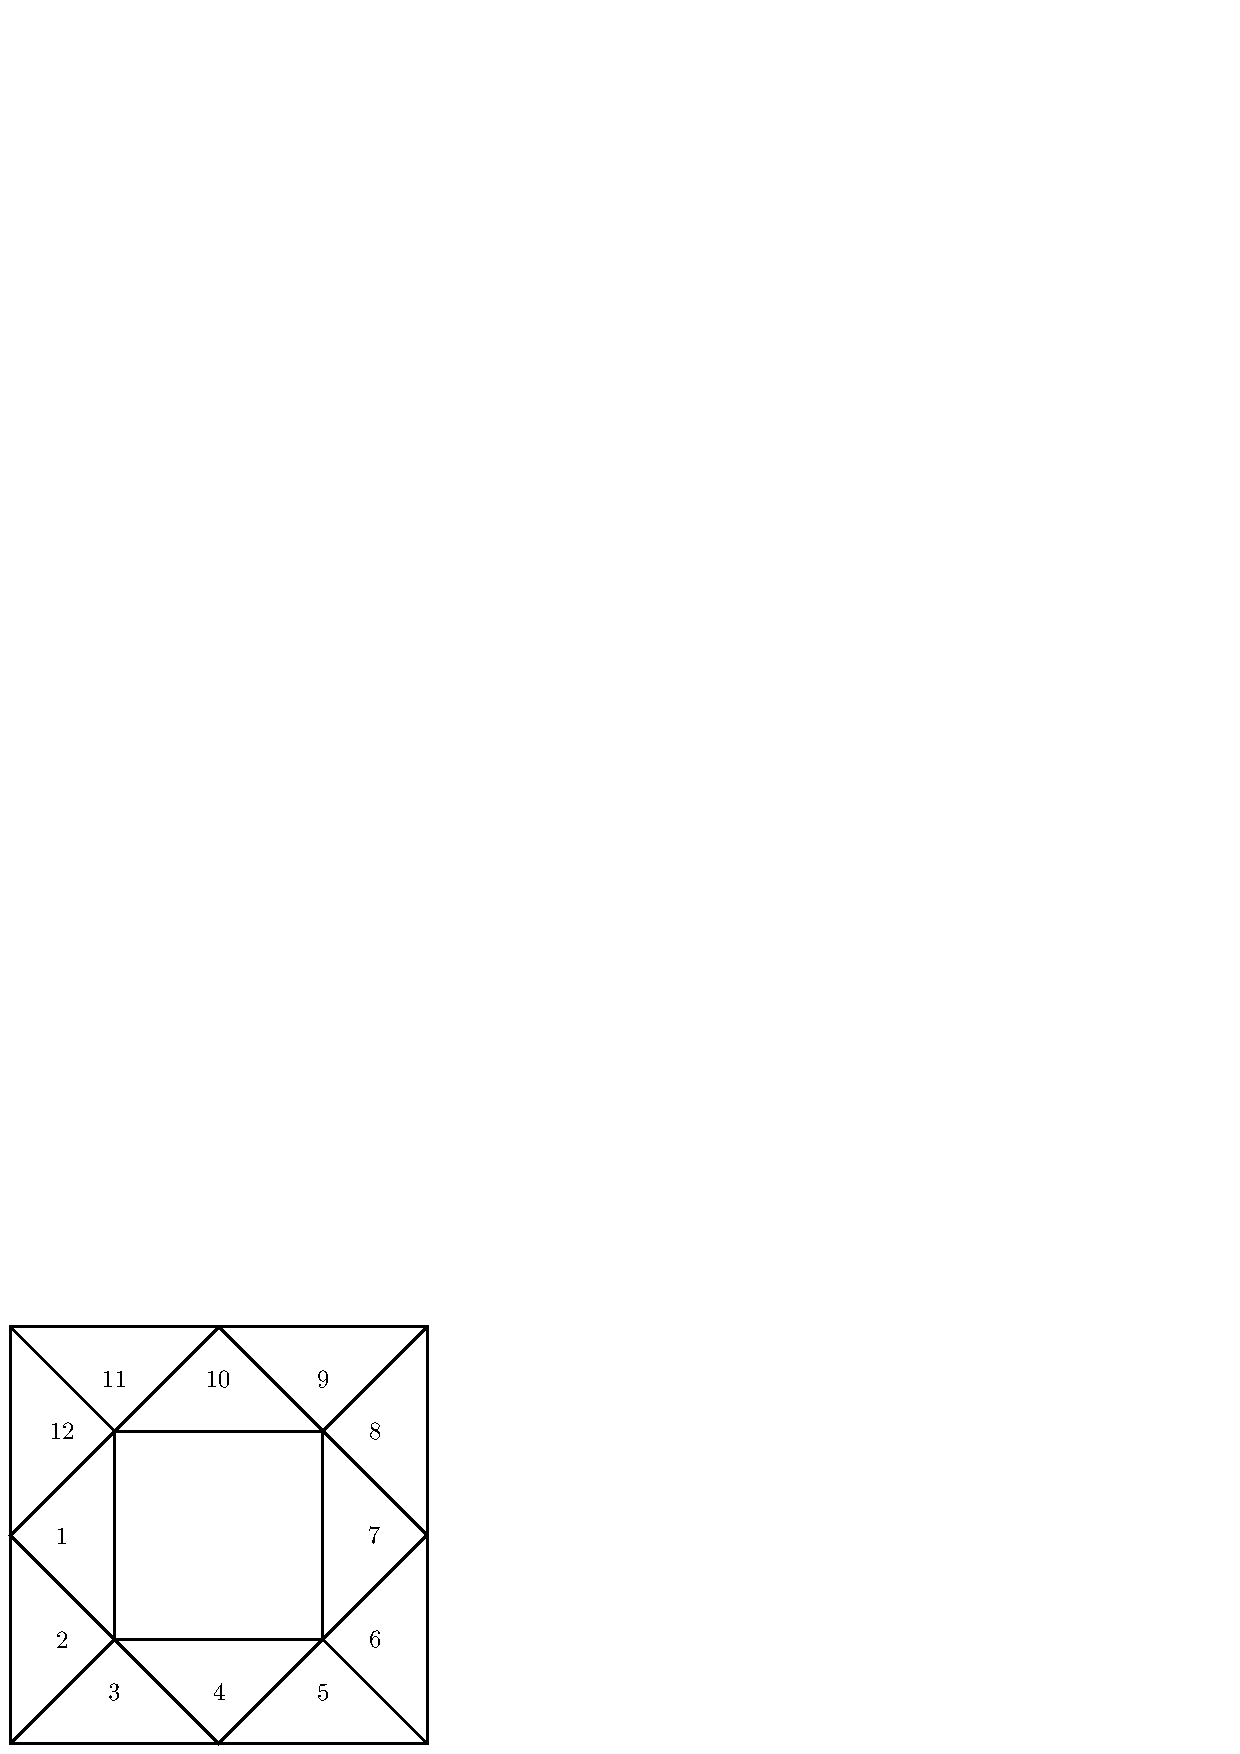
\includegraphics{./images/illus296}}
\end{figure*}
house, and so on. The dividing lines were termed \emph{cusps}\index
{Cusps, Astrological}: the
line between the houses $12$ and $1$ was called the cusp of
the first house, the line between the houses $1$ and $2$ was called
the cusp of the second house, and so on, finally the line
between the houses $11$ and $12$ was called the cusp of the
twelfth house. Each house had also a name of its own---thus
the first house was called the ascendant house, the eighth
house was called the house of death, and so on---but as
these names are immaterial for my purpose I shall not define
them.

Next, the positions which the various astrological signs
and planets had occupied at some definite time and place (for
\PG----File: 297.png------------------------------------------------------
instance, the time and place of birth of the native, if his nativity
was being cast) were marked on the celestial sphere. This
sphere was divided into twelve equal spaces by great circles
drawn through the zenith, the angle between any two consecutive
circles being $30^{\circ}$. The first circle was drawn through the
East point, and the space between it and the next circle towards
the North corresponded to the first house, and sometimes
was called the first house. The next space, proceeding from East
to North, corresponded to the second house, and so on. Each
of the twelve spaces between these circles corresponded to
one of the twelve houses, and each of the circles to one of
the cusps.

In delineating\index{HoroscopeRulesCast@\nobreak--- Rules to cast}\footnote
{Raphael, pp.~118--131.} a horoscope, it was usual to begin by
inserting the zodiacal signs. A zodiacal sign\index
{Zodiac, Signs in Astrology} extends over $30^{\circ}$,
and was marked on the cusp which passed through it: by its
side was written a number indicating the distance to which its
influence extended in the earlier of the two houses divided by
the cusp. Next the position of the planets in these signs were
calculated, and each planet was marked in its proper house
and near the cusp belonging to the zodiacal sign in which
the planet was then situated: it was followed by a number
indicating its right ascension measured from the beginning of
the sign. The name of the native and the date for which the
horoscope was cast were inserted usually in the central square.
The \hyperlink{illus:307}{diagram} near the end of this chapter is a
facsimile of the horoscope of Edward~VI\index{Edward VI} as cast by Cardan
and will serve as an illustration of the above remarks.

We are now in a position to explain how a horoscope was
\emph{read}\index{HoroscopesRulesRead@\nobreak--- Rules to read|(} or interpreted.
Each house was associated with certain
definite questions and subjects, and the presence or absence in
that house of the various signs and planets gave the answer to
these questions or information on these subjects.

These questions cover nearly every point on which information
would be likely to be sought. They may be classified
roughly as follows. For the answer, so far as it concerns the
\PG----File: 298.png------------------------------------------------------
native, to all questions connected with his life and health, look
in house~1; for questions connected with his wealth, refer to
house~2; for his kindred and communications to him, refer to
3; for his parents and inheritances, refer to 4; for his children
and amusements, refer to 5; for his servants and illnesses,
refer to 6; for his marriage and amours, refer to 7; for his
death, refer to 8; for his learning, religion and travels, refer
to 9; for his trade and reputation, refer to 10; for his friends,
refer to 11; and finally for questions connected with his
enemies, refer to house 12.

\phantomsection
\addcontentsline{toc}{subsection}{Planets and their significations}
I proceed to describe briefly the influences of the planets%
\index{PlanetsA@Planets (astrological)}%
\index{PlanetsS@\nobreak--- Signification of|(},
and shall then mention those of the zodiacal signs; I should
note however that in practice the signs were in many respects
more influential than the planets.

The astrological ``planets''\index{Astrological Planets} were seven in
number, and included the Sun and the Moon. They were Saturn or the
Great Infortune, Jupiter or the Great Fortune, Mars or the
Lesser Infortune, the Sun, Venus or the Lesser Fortune,
Mercury, and the Moon: the above order being that of their
apparent times of rotation round the earth.

Each of them had a double signification. In the first place
it impressed certain characteristics, such as good fortune,
feebleness,~\&c., on the dealings of the native with the subjects
connected with the house in which it was located; and in the
second place it imported certain objects into the house which
would affect the dealings of the native with the subjects of
that house.

To describe the exact influence of each planet in each
house would involve a long explanation, but the general effect
of their presence may be indicated roughly as follows\footnote
{Raphael, pp.~70--90; pp.~204--209.}. The
presence of Saturn is malignant: that of Jupiter is propitious:
that of Mars is on the whole injurious: that of the Sun
indicates respectability and moderate success: that of Venus
is rather favourable: that of Mercury implies rapid practical
action: and lastly the presence of the Moon merely faintly
\PG----File: 299.png------------------------------------------------------
reflects the influence of the planet nearest her, and suggests
rapid changes and fickleness. Besides the planets, the Moon's
nodes and some of the more prominent fixed stars\footnote
{Raphael, pp.~129--131,} also had certain influences.

These vague terms may be illustrated by taking a few
simple cases.

For example, in casting a nativity, the life, health, and
general career of the native were determined by the first or
ascendant house, whence comes the expression that a man's
fortune is in the ascendant. Now the most favourable planet
was Jupiter. Therefore, if at the instant of birth Jupiter was
in the first house, the native might expect a long, happy,
healthy life; and being born under Jupiter he would have a
``jovial'' disposition. On the other hand, Saturn was the most
unlucky of all the planets, and was as potent as malignant. If
at the instant of birth he was in the first house, his potency
might give the native a long life, but it would be associated
with an angry and unhappy temper, a spirit covetous, revengeful,
stern, and unloveable, though constant in friendship
no less than in hate, which was what astrologers meant by a
``saturnine'' character. Similarly a native born under Mercury,
that is, with Mercury in the first house, would be of a mercurial
nature, while anyone born under Mars would have a martial
bent.

Moreover it was the prevalent opinion that a jovial person
would have his horoscope affected by Jupiter, even if that
planet had not been in the ascendant at the time of birth.
Thus the horoscope of an adult depended to some extent on his
character and previous life. It is hardly necessary to point
out how easily this doctrine enabled an astrologer to make the
prediction of the heavens agree with facts that were known
or probable.

In the same way the other houses are affected. For instance,
no astrologer, who believed in the art, would have
wished to start on a long journey when Saturn was in the
\PG----File: 300.png-----------------------------------------------------
ninth house or house of travels; and, if at the instant of birth
Saturn was in that house, the native always would incur
considerable risk on his journeys.

Moreover every planet was affected to some extent by its
aspect (conjunction, opposition, or quadrature) to every other
planet according to elaborate rules\footnote
{Raphael, pp. 132--170.} which depended on their
positions and directions of motion: in particular the angular
distance between the Sun and the Moon---sometimes known
as the ``part of fortune''---was regarded as specially important,
and this distance affected the whole horoscope. In general,
conjunction was favourable, quadrature unfavourable, and
opposition ambiguous.

Each planet not only influenced the subjects in the house in
which it was situated, but also imported certain objects into
the house. Thus Saturn was associated with grandparents,
paupers, beggars, labourers, sextons, and gravediggers. If, for
example, he was present in the fourth house, the native might
look for a legacy from some such person; if he was present
in the twelfth house, the native must be careful of the consequences
of the enmity of any such person; and so on.

Similarly Jupiter was associated generally with lawyers,
priests, scholars, and clothiers; but, if he was conjoined with a
malignant planet, he represented knaves, cheats, and drunkards.
Mars indicated soldiers (or, if in a watery sign, sailors on ships
of war), masons, doctors, smiths, carpenters, cooks, and tailors;
but, if afflicted with Mercury or the Moon, he denoted the
presence of thieves. The Sun implied the action of kings,
goldsmiths, and coiners; but, if afflicted by a malignant planet,
he denoted false pretenders. Venus imported musicians, embroiderers,
and purveyors of all luxuries; but, if afflicted,
prostitutes and bullies. Mercury imported astrologers, philosophers,
mathematicians, statesmen, merchants, travellers, men
of intellect, and cultured workmen; but, if afflicted, he signified
the presence of pettifoggers, attorneys, thieves, messengers,
\PG----File: 301.png-----------------------------------------------------
footmen, and servants. Lastly, the presence of the Moon
introduced sailors and those engaged in inferior offices\index
{PlanetsS@\nobreak--- Signification of|)}.

\phantomsection
\addcontentsline{toc}{subsection}{Zodiacal signs and their significations}
I come now to the influence and position of the zodiacal\index
{Zodiac, Signs in Astrology}
signs. So far as the first house was concerned, the sign of the
zodiac which was there present was even more important than
the planet or planets, for it was one of the most important
indications of the durations of life.

Each sign was connected with certain parts of the body---\Eg\
Aries influenced the head, neck and shoulders---and that
part of the body was affected according to the house in which
the sign was. Further each sign was associated with certain
countries and connected the subjects of the house in which the
sign was situated with those countries: \Eg\ Aries was
associated especially with events in England, France, Syria,
Verona, Naples,~\&c.

The sign in the first house determined also the character
and appearance of the native\footnote
{Raphael, pp. 61--69.}. Thus the character of a native
born under Aries (\textit{m}) was passionate; under Taurus (\textit{f}) was
dull and cruel; under Gemini (\textit{m}) was active and ingenious;
under Cancer (\textit{f}) was weak and yielding; under Leo (\textit{m}) was
generous, resolute, and ambitious; under Virgo (\textit{f}) was sordid
and mean; under Libra (\textit{m}) was amorous and pleasant; under
Scorpio (\textit{f}) was cold and reserved; under Sagittarius (\textit{m})
was generous, active, and jolly; under Capricorn (\textit{f}) was weak and
narrow; under Aquarius (\textit{m}) was honest and steady; and under
Pisces (\textit{f}) was phlegmatic and effeminate.

Moreover the signs were regarded as alternately masculine
and feminine, as indicated above by the letters \textit{m} or \textit{f}
placed after each sign. A masculine sign is fortunate, and all planets
situated in the same house have their good influence rendered
thereby more potent and their unfavourable influence mitigated.
But all feminine signs are unfortunate, their direct effect is evil,
and they tend to nullify all the good influence of any planet
which they afflict (\IE\ with which they are connected), and to
increase all its evil influences, while they also import an element
\PG----File: 302.png------------------------------------------------------
of fickleness into the house and often turn good influences into
malignant ones. The precise effect of each sign was different
on every planet\index{HoroscopesRulesRead@\nobreak--- Rules to read|)}.

\phantomsection
\addcontentsline{toc}{section}{Knowledge that rules were worthless}
I think the above account is sufficient to enable the reader
to form a general idea of the manner in which a horoscope was
cast and interpreted, and I do not propose to enter into further
details. This is the less necessary as the rules---especially as
to the relative importance to be assigned to various planets
when their influence was conflicting---were so vague that astrologers
had little difficulty in finding in the horoscope of a client
any fact about his life of which they had information or any
trait of character which they suspected him to possess.

That this vagueness was utilized by quacks is notorious,
but no doubt many an astrologer in all honesty availed himself
of it, whether consciously or unconsciously. It must be remembered
also that the rules were laid down at a time when men
were unacquainted with any exact science, with the possible
exception of mathematics, and further that, if astrology had
been reduced to a series of inelastic rules applicable to all horoscopes,
the number of failures to predict the future correctly
would have rapidly led to a recognition of the folly of the art.
As it was, the failures were frequent and conspicuous enough
to shake the faith of most thoughtful men. Moreover it was a
matter of common remark that astrologers showed no greater
foresight in meeting the difficulties of life than their neighbours,
while they were neither richer, wiser, nor happier for
their supposed knowledge. But though such observations were
justified by reason they were often forgotten in times of difficulty
and danger. A prediction of the future and the promise
of definite advice as to the best course of action, revealed by the
heavenly bodies themselves, appealed to the strongest desires of
all men, and it was with reluctance that the futility of the
advice was gradually recognized.

The objections to the scheme had been stated clearly by
several classical writers. Cicero\index{Cicero on Astrology}\footnote
{Cicero, \textit{De Divinatione}, \textsc{ii}, 42.} pointed out that
not one of
\PG----File: 303.png------------------------------------------------------
the futures foretold for Pompey\index{Pompey}, Crassus\index{Crassus},
and Caesar\index{Caesar, Julius}\index{Julius Caesar} had been
verified by their subsequent lives, and added that the planets,
being almost infinitely distant, cannot be supposed to affect
us. He also alluded to the fact, which was especially pressed by
Pliny\index{Pliny}\footnote
{Pliny, \textit{Historia Naturalis}, \textsc{vii}, 49; \textsc{xxix}, 1.},
that the horoscopes of twins are practically identical
though their careers are often very different, or as Pliny put it,
every hour in every part of the world are born lords and slaves,
kings and beggars.

In answer to the latter obvious criticism astrologers replied
by quoting the anecdote of Publius Nigidius Figulus\index
{Figulus on Astrology}\index{Nigidius on Astrology}, a
celebrated Roman astrologer of the time of Julius Caesar. It
is said that when an opponent of the art urged as an objection
the different fates of persons born in two successive instants,
Nigidius bade him make two contiguous marks on a potter's
wheel, which was revolving rapidly near them. On stopping
the wheel, the two marks were found to be far removed from
each other. Nigidius received the name of Figulus, the
potter, in remembrance of this story, but his argument, says
St~Augustine\index{Augustine on Astrology}\footnote
{St~Augustine, \textit{De Civitate Dei}, bk.~\textsc{v}, chap.~iii;
\textit{Opera omnia}, ed.\ Migne, vol.~\textsc{vii}, p.~143.}, who
gives us the narrative, was as fragile as
the ware which the wheel manufactured.

On the other hand Seneca\index{Seneca on Astrology} and Tacitus\index
{Tacitus on Astrology} may be cited as
being on the whole favourable to the claims of astrology,
though both recognized that it was mixed up with knavery and
fraud. An instance of successful prediction which is given
by the latter of these writers\footnote
{\textit{Annales}, \textsc{vi}, 22: quoted by Whewell\index{Whewell, W.},
\textit{History of the Inductive Sciences}, vol.~\textsc{i}, p.~313.}
may be used more correctly as
an illustration of how the ordinary professors of the art varied
their predictions to suit their clients and themselves. The
story deals with the first introduction of the astrologer Thrasyllus\index
{Thrasyllus on Astrology} to the emperor Tiberius\index
{Tiberius on Astrology}. Those who were brought to
Tiberius on any important matter were admitted to an interview
in an apartment situated on a lofty cliff in the island
\PG----File: 304.png------------------------------------------------------
of Capreae. They reached this place by a narrow path overhanging
the sea, accompanied by a single freedman of great
bodily strength; and on their return, if the emperor had conceived
any doubts of their trustworthiness, a single blow buried
the secret and its victim in the ocean. After Thrasyllus had,
in this retreat, stated the results of his art as they concerned
the emperor, the latter asked the astrologer whether he had
calculated how long he himself had to live. The astrologer
examined the aspect of the stars, and while he did this showed,
as the narrative states, hesitation, alarm, increasing terror, and
at last declared that the present hour was for him critical,
perhaps fatal. Tiberius\index{Tiberius on Astrology} embraced him, and told
him he was right in supposing he had been in danger but that he should
escape it; and made him thenceforth a confidential counsellor.
But Thrasyllus\index{Thrasyllus on Astrology} would have been but a sorry
astrologer had he not foreseen such a question and prepared an answer which
he thought fitted to the character of his patron.

A somewhat similar story is told\footnote
{\textit{Personal Characteristics from French History}, by Baron
F.~Rothschild\index{Rothschild, F.},
London, 1896, p.~10. The story was introduced by Sir Walter
Scott\index{Scott, Sir Walter} in Quentin Durward (chap.~\textsc{xv}).}
of Louis~XI\index{Louis XI of France} of France.
He sent for a famous astrologer whose death he was meditating,
and asked him to show his skill by foretelling his own future.
The astrologer replied that his fate was uncertain, but it was
so inseparably interwoven with that of his questioner that the
latter would survive him but by a few hours, whereon the
superstitious monarch not only dismissed him uninjured, but
took steps to secure his subsequent safety. The same anecdote
is also related of a Scotch student who, being captured by
Algerian pirates, predicted to the Sultan that their fates
were so involved that he should predecease the Sultan by
only a few weeks. This may have been good enough for a
barbarian, but with a civilized monarch it probably would in
most cases be less effectual, as certainly it is less artistic,
than the answer of Thrasyllus.

\PG----File: 305.png------------------------------------------------------
\medskip
\phantomsection
\addcontentsline{toc}{section}{Notable instances of horoscopy}
I may conclude by mentioning a few notable cases of horoscopy.

\phantomsection
\addcontentsline{toc}{subsection}{Lilly's prediction of the Great Fire
and Plague}
Among the most successful instances of horoscopy enumerated
by Raphael\footnote
{\textit{Manual of Astrology}, p.~37.} is one by W.~Lilly\index
{Lilly on Astrology}, given in his \textit{Monarchy
or No Monarchy}, published in 1651, in which he predicted a
plague in London so terrible that the number of deaths should
exceed the number of coffins and graves, to be followed by ``an
exorbitant fire.'' The prediction was amply verified in 1665
and 1666. In fact Lilly's success was embarrassing, for the
Committee of the House of Commons, which sat to investigate
the causes of the fire and ultimately attributed it to the papists,
thought that he must have known more about it than he
chose to declare, and on Oct.~25, 1666, summoned him before
them. I may add that Lilly proved himself a match for his
questioners.

\phantomsection
\addcontentsline{toc}{subsection}{Flamsteed's guess}
An even more curious instance of a lucky hit is told of
Flamsteed\index{Flamsteed on Astrology}\footnote
{The story, though in a slightly different setting, is given in \textit{The
London Chronicle}, Dec.~3, 1771, and it is there stated that Flamsteed
attributed the result to the direct action of the devil.},
the first astronomer royal. It is said that an
old lady who had lost some property wearied Flamsteed by
her perpetual requests that he would use his observatory to
discover her property for her. At last, tired out with her importunities,
he determined to show her the folly of her demand
by making a prediction, and, after she had found it false, to
explain again to her that nothing else could be expected.
Accordingly he drew circles and squares round a point that
represented her house and filled them with all sorts of mystical
symbols. Suddenly striking his stick into the ground he said,
``Dig there and you will find it.'' The old lady dug in the spot
thus indicated, and found her property; and it may be conjectured
that she believed in astrology for the rest of her life.

Perhaps the belief that the royal observatory was built for
such purposes may be still held, for De~Morgan\index
{DeMorgan@De Morgan, A.}, writing in
1850, says that ``persons still send to Greenwich to have their
\PG----File: 306.png-------------------------------------------------------
fortunes told, and in one case a young gentleman wrote to
know who his wife was to be, and what fee he was to remit.''

It is easier to give instances of success in horoscopy than of
failure. Not only are all ambiguous predictions esteemed to
be successful, but it is notorious that prophecies which have
been verified by the subsequent course of events are remembered
and quoted, while the far more numerous instances in which the
prophecies have been falsified are forgotten or passed over in
silence.

\phantomsection
\addcontentsline{toc}{subsection}{Cardan's horoscope of Edward VI}
As exceptionally well-authenticated instances of failures
I may mention the twelve cases collected by Cardan\index{Cardan|(} in his
\textit{Geniturarum Exempla}. These are good examples because
Cardan was not only the most eminent astrologer of his time,
but was a man of science, and perhaps it is not too much to say
was accustomed to accurate habits of thought; moreover, as far
as I can judge, he was perfectly honest in his belief in astrology.
To English readers the most interesting of these is the horoscope
of Edward~VI\index{Edward VI|(} of England, the more so as Cardan has left
a full account of the affair, and has entered into the reasons of
his failure to predict Edward's death.

To show how Cardan came to be mixed up in the transaction
I should explain that in 1552 Cardan went to Scotland to
prescribe for John Hamilton\index{Hamilton, Archbishop}, the archbishop of
St~Andrews, who was ill with asthma and dropsy and about whose treatment
the physicians had disagreed\footnote
{Luckily they left voluminous reports on the case and the proper
treatment for it. The only point on which there was a general agreement
was that the phlegm, instead of being expectorated, collected in his
Grace's brains, and that thereby the operations of the intellect were
impeded. Cardan was celebrated for his success in lung diseases, and his
remedies were fairly successful in curing the asthma. His fee was $500$
crowns for travelling expenses from Pavia, $10$ crowns a day, and the
right to see other patients; the archbishop actually gave him $2300$ crowns
in money and numerous presents in kind; his fees from other persons
during the same time must have amounted to about an equal sum (see
Cardan's \textit{De Libris Propriis}, ed.\ 1557, pp.~159--175; \textit
{Consilia Medica}, \textit{Opera}, vol.~\textsc{ix}, pp.~124--148;
\textit{De Vita Propria}, ed.\ 1557, pp.~138, 193 \etseq).}.
On his return through
\PG----File: 307.png-------------------------------------------------------
London, Cardan stopped with Sir John Cheke\index{Cheke, Sir John}, the
Professor of Greek at Cambridge, who was tutor to the young king. Six
months previously, Edward had been attacked by measles and
small-pox which had made his health even weaker than before.
The king's guardians were especially anxious to know how long
he would live, and they asked Cardan to cast Edward's nativity
with particular reference to that point.

The Italian was granted an audience in October, of which
he wrote a full account in his diary, quoted in the \textit{Geniturarum
Exempla}. The king, says he\footnote
{I quote from Morley's\index{Morley on Cardan} translation, vol.~\textsc{ii},
p.~135 \etseq}, was ``of a stature somewhat
below the middle height, pale faced, with grey eyes, a grave
aspect, decorous, and handsome. He was rather of a bad habit
of body than a sufferer from fixed diseases, and had a somewhat
projecting shoulder-blade.'' But, he continues, he was a
boy of most extraordinary wit and promise. He was then
but fifteen years old and he was already skilled in music and
dialectics, a master of Latin, English, French, and fairly proficient
\begin{figure*}[htb]
\centerline{\hypertarget{illus:307}{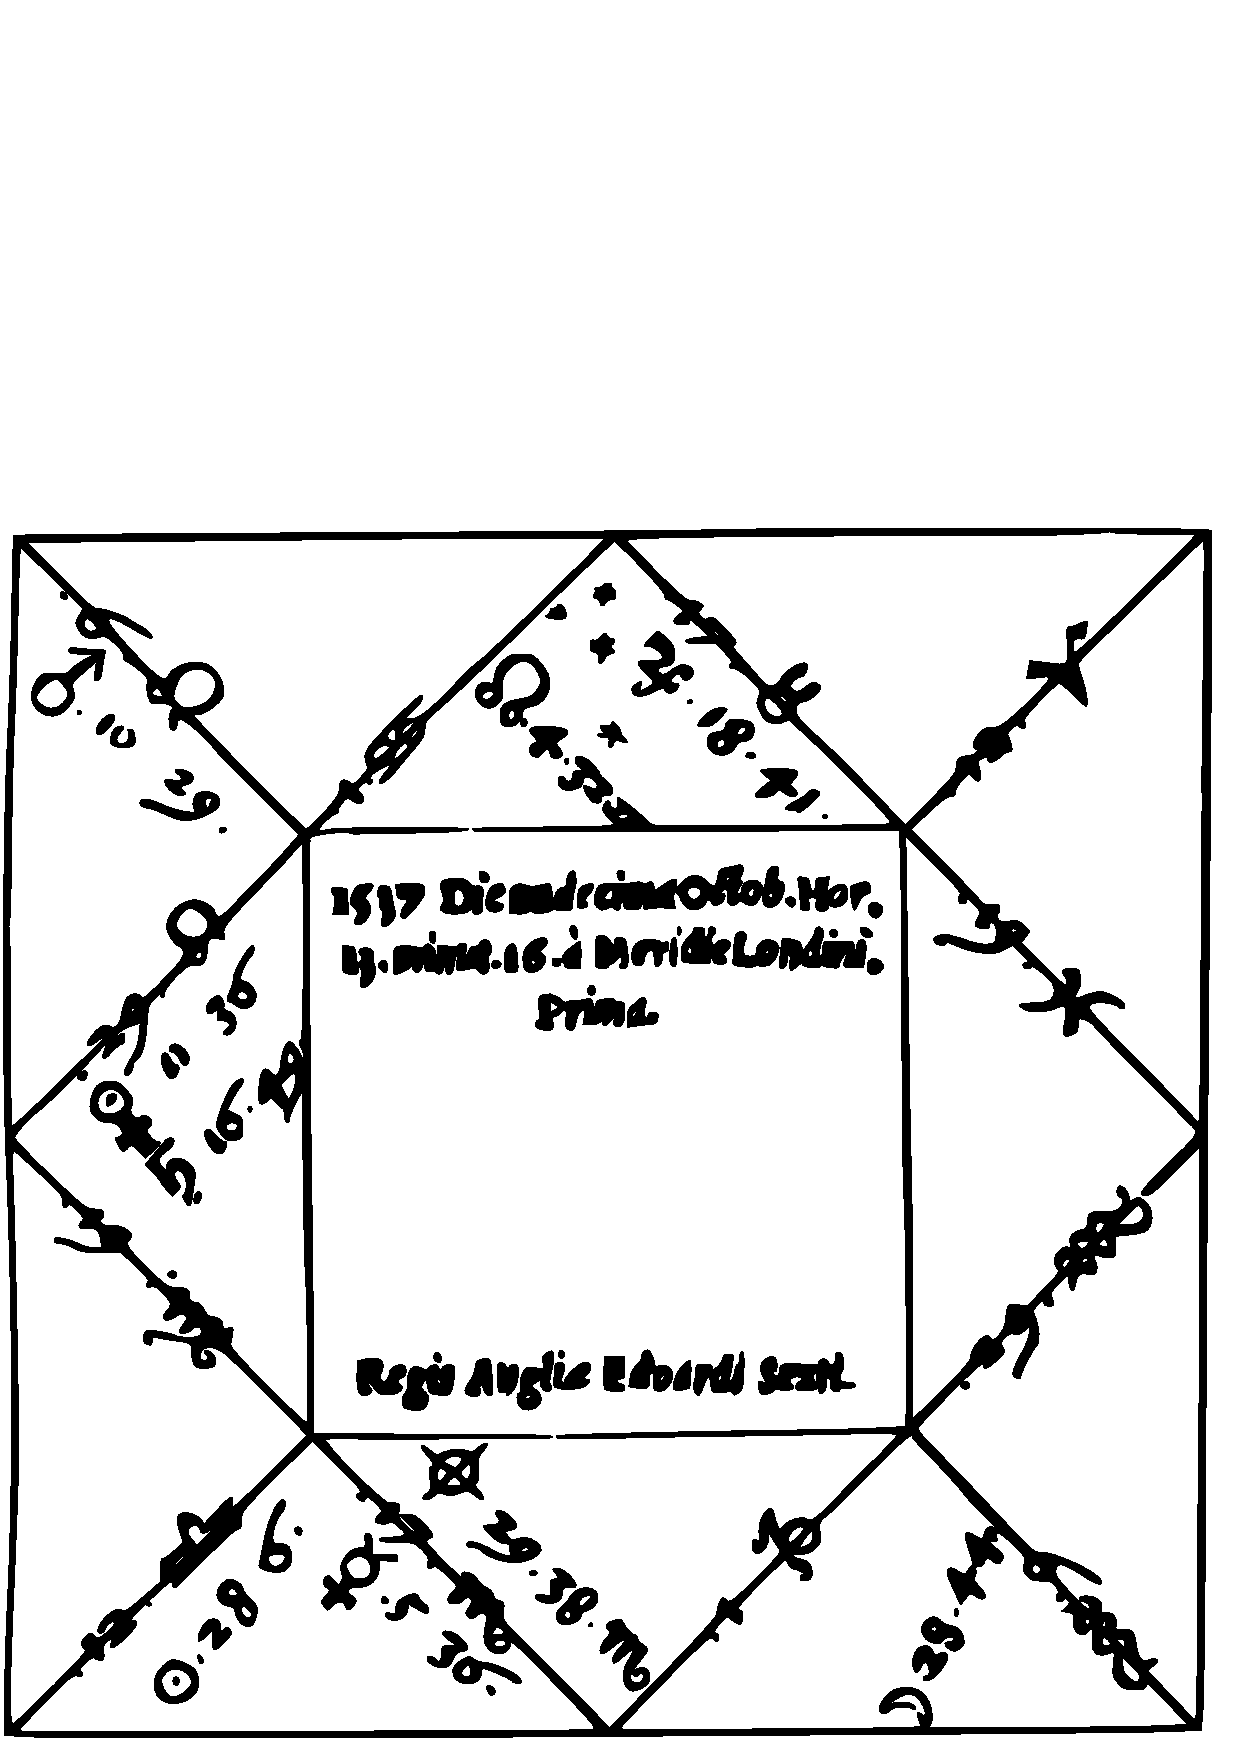
\includegraphics
[height=\ifPaper9cm\else.7\textheight\fi]{./images/illus307}\index
{EdwardHoro@\protect\nobreak--- Horoscope of}\index
{HoroscopesExample@\protect\nobreak--- Example of}}}\label{illus:307}
\end{figure*}
\PG----File: 308.png------------------------------------------------------
in Greek, Italian, and Spanish. He ``filled with the
highest expectation every good and learned man, on account of
his ingenuity and suavity of manners\textellipsis. When a royal gravity
was called for, you would think that it was an old man you saw,
but he was bland and companionable as became his years. He
played upon the lyre, took concern for public affairs, was liberal
of mind, and in these respects emulated his father\index
{Henry VIII of England}, who, while he
studied to be [too] good, managed to seem bad.'' And in another
place\footnote{\textit{De Rerum Varietate}, p.~285.}
he describes him as ``that boy of wondrous hopes.'' At
the close of the interview Cardan begged leave to dedicate to
Edward a work on which he was then engaged. Asked the
subject of the work, Cardan replied that he began by showing
the cause of comets. The subsequent conversation, if it is
reported correctly, shows good sense and considerable logical
skill on the part of the young king.

I have reproduced \vpageref{illus:307} a facsimile of Cardan's original
drawing of Edward's horoscope. The horoscope was cast and
read with unusual care. I need not quote the minute details
given about Edward's character and subsequent career, but
obviously the predictions were founded on the impressions derived
from the above-mentioned interview. The conclusion
about his length of life was that he would certainly live past
middle age, though after the age of 55 years 3 months and
17 days various diseases would fall to his lot\footnote
{\textit{Geniturarum Exempla}, p.~19.\label{ibid:16}}.

In the following July the king died\index{Edward VI|)}, and Cardan felt it
necessary for his reputation to explain the cause of his error.
The title of his dissertation is \emph{Quae post consideravi de
eodem}\footnote{\Ibidref{ibid:16}{\textit{Geniturarum Exempla}}, p.~23.}.
In effect his explanation is that a weak nativity can never
be predicted from a single horoscope, and that to have ensured
success he must have cast the nativity of every one with whom
Edward had come intimately into contact; and, failing the
necessary information to do so, the horoscope could be regarded
only as a probable prediction\index{Cardan|)}.

\PG----File: 309.png------------------------------------------------------
This was the argument usually offered to account for non-success.
A better defence would have been the one urged
by Raphael\footnote{\textit{The Familiar Astrologer}, London, 1832, p.~248.}
and by Southey\index{Southey on Astrology}\footnote
{\textit{The Doctor}, chap.~92.} that there might be other
planets unknown to the astrologer which had influenced
the horoscope, but I do not think that medieval astrologers
assigned this reason for failure.

I have not alluded to the various adjuncts of the art, but
astrologers so frequently claimed the power to be able to raise
spirits\index{Spirits, Raising} that perhaps I may be pardoned for remarking
that I believe some of the more important and elaborate of these
deceptions were effected not infrequently by means of a magic
lantern, the pictures being sometimes thrown on to a mirror,
and at other times on to a thick cloud of smoke which caused
the images to move and finally disappear in a fantastic way
capable of many explanations\footnote
{See \Eg\ the life of Cellini\index{Cellini}, chap.~\textsc{xiii},
Roscoe's translation, pp.~144-146. See also Sir David Brewster's\index
{Brewster, Sir David} \textit{Letters on Natural Magic}.}.

I would conclude by repeating again that though the
practice of astrology was so often connected with impudent
quackery, yet one ought not to forget that nearly every
physician and man of science in medieval Europe was an
astrologer. These observers did not consider that its rules
were definitely established, and they laboriously collected much
of the astronomical evidence that was to crush their art. Thus,
though there never was a time when astrology was not practised
by knaves, there was a period of intellectual development when
it was honestly accepted as a difficult but a real science.

\PG----File: 310.png-------------------------------------------------------




% CHAPTER XI

\chapter{Cryptographs and Ciphers.}


\textsc{The} art of constructing cryptographs or
ciphers---intelligible\chapindex{Ciphers@\textsc{Ciphers}}
\chapindex{Cryptography@\textsc{Cryptography}}%
\chapindex{Secret@\textsc{Secret Communications}}%
to those who know the key and unintelligible to others---has
been studied for centuries. Their usefulness on certain
occasions, especially in time of war, is obvious, while it may
be a matter of great importance to those from whom the key
is concealed to discover it. But the romance connected with
the subject, the not uncommon desire to discover a secret, and
the implied challenge to the ingenuity of all from whom the
key is hidden, have attracted to the subject the attention of
many to whom its utility is a matter of indifference.

The leading authorities on the subject, few of which are
less than a century old, are enumerated in an article by J.E.~Bailey\index
{Bailey, J.E.} in the ninth edition of the \textit{Encyclopaedia Britannica},
and references to various historic ciphers are there given.
My knowledge of the subject, however, is limited to ciphers
which I have met with in the course of casual reading, and I
prefer to discuss the subject as it has presented itself to me,
with no attempt to make it historically complete and no
reference to other authorities. In fact the theory of the
subject is not sufficiently important to make it worth while
to try to deal with it historically or exhaustively.

Most writers use the words cryptograph and cipher as
synonymous. I employ them, however, with different meanings,
which I proceed to define.

\PG----File: 311.png-------------------------------------------------------
\phantomsection
\addcontentsline{toc}{section}{A Cryptograph. Definition. Illustration}
A cryptograph may be defined\index
{Cryptographs, Def@\textsc{Cryptographs}, Definition of}
as a manner of writing in
which the letters or symbols employed are used in their
normal sense, but are so arranged that the communication is
intelligible only to those possessing the key. The word is
sometimes used to denote the communication made. A simple
example is a communication in which every word is spelt
backwards. Thus:
\[
\text{\emph{ymene deveileb ot eb gniriter troper noitisop no ssorc daor.}}
\]

\phantomsection
\addcontentsline{toc}{section}{A Cipher. Definition. Illustration}
A cipher may be defined\index{Ciphers, Definition@\nobreak--- Definition of}
as a manner of writing by
characters arbitrarily invented or by an arbitrary use of
letters, words, or characters in other than their ordinary
sense, intelligible only to those possessing the key. The
word is sometimes used to denote the communication made.
A simple example is when each letter is replaced by the
one that immediately follows it in the natural order of the
alphabet, \emph{a} being replaced by \emph{b}, \emph{b} by \emph{c},
and so on, and finally
\emph{z} by \emph{a}. In this cipher the above message would read:
\[
\text{\emph{fofnz cfmjfwfe up cf sfujsjoh sfqpsu qptjujpo po dsptt spbe.}}
\]

\phantomsection
\addcontentsline{toc}{section}{Essential Features of Cryptographs
and Ciphers}
In both cryptographs and ciphers the essential feature is
that the communication may be freely given to all the world
though it is unintelligible save to those who possess the key.
The key must not be accessible to anyone, and if possible it
should be known only to those using the cryptograph or
cipher. The art of constructing a cryptograph lies in the
concealment of the proper order of the essential letters or
words: the art of constructing a cipher lies in concealing
what letters or words are represented by the symbols used.
In an actual communication cipher symbols may be arranged
cryptographically, and thus further hinder a reading of the
message. Thus the message given above would read in a
cryptographic cipher as
\[
\text{\emph{znfof efwfjmfc pu fc hojsjufs uspqfs opjujtpq op ttpsd ebps.}}
\]
If the message were sent in Latin or some foreign language it
would further diminish the chance of it being read by a
\PG----File: 312.png------------------------------------------------------
stranger through whose hands it passed. But I may confine
myself to messages in English, and for the present to simple
cryptographs and ciphers.

A communication in cryptograph or cipher must be in
writing or in some permanent form. Thus to make small
muscular movements---such, \Eg, as talking on the fingers,
or breathing long and short in the Morse dot and dash system,
or making use of pre-arranged signs by a fan or stick, or
flashing signals by light---do not here concern us.

Again, the mere fact that the message is concealed or
conveyed secretly does not make it a cryptograph or cipher.
The majority of stories dealing with secret communications
are concerned with the artfulness with which the message
is concealed or conveyed and have nothing to do with
cryptographs or ciphers. Many of the ancient instances of
secret communication are of this type\footnote
{A long list of classical authorities for different devices used in
ancient times for concealing messages is given in \textit{Mercury} by
J.~Wilkins\index{Wilkins on Ciphers}, London, 1641, pp.~27--36.}.
Illustrations are to
be found in messages conveyed by pigeons, or wrapped round
arrows shot over the head of a foe, or written on the paper
wrapping of a cigarette, or the use of ink which becomes
visible only when the recipient treats the paper on which it
is written by some chemical or physical process.

Again, a communication in a foreign language or in any
recognized notation like shorthand is not an instance of a
cipher. A letter in Chinese or Polish or Russian might be
often used for conveying a secret message from one part of
England to another, but it fails to fulfil our test that if
published to all the world it would be concealed from everyone,
unless submitted to some special investigation. On the other
hand, in practice, foreign languages or systems of shorthand
which are but little known may serve to conceal a communication
better than an easy cipher, for in the last case
the key may be found with but little trouble, while in the
other cases, though the key may be accessible, it is probable
\PG----File: 313.png-------------------------------------------------------
that there are only a few who know where to look for it.
An illustration of this is afforded by the system used by
Pepys in writing his Diary which is further alluded to below.

\phantomsection
\addcontentsline{toc}{section}{Cryptographs of Three Types.
Illustrations}\markright{Cryptographs}
I proceed to enumerate some of the better known types of
cryptographs. There are at least three distinct types. The\index
{Cryptographs, Three@\nobreak--- Three types of|(}
first type comprises those in which the order of the letters
is changed in some pre-arranged manner. The second type
comprises those in which the concealment is due to the introduction
of non-significant letters. The third type comprises
those in which the letters used are written in fragments.
The types are not exclusive, and any particular cryptograph
may comprise the distinctive feature of two or all the types.

\phantomsection
\addcontentsline{toc}{subsection}{Order of letters re-arranged}
A cryptograph of the first type is one in which the
successive letters of the message are re-arranged in some
pre-determined manner.

One of the most obvious cryptographs of this type is to
write each word or the message itself backwards. He would,
however, be a careless reader who could be deceived by this.
Here is an instance in which the whole message is written
backwards:
\[
\text{\emph{tsop yb tnes tnemeerga fo seniltuo smret ruo tpecca yeht.}}
\]
In such a case it is unnecessary to indicate the division into
words by leaving spaces between them, and we might divide
the letters artificially, as thus:
\[
\text{\emph{Ts opybtne stne meer gafos eniltu osmret ruot peccaye ht.}}
\]

Systems of this kind which depend on altering the places
of letters or lines in some pre-arranged manner have always
been common. I quote a couple of instances\footnote
{\textit{Mercury, or the Secret and Swift Messenger}, by
\hypertarget{footnote:wilkins}{J.~Wilkins}, London,
1641, pp.~50--52.} from Wilkins's\index{Wilkins on Ciphers}
book to which I have already referred---it was a work which
seems to have been studied diligently by many of those who
took part in the civil disturbances of the 17th century, and
gives an excellent account of some of the easier systems of
cryptographs and ciphers.

\PG----File: 314.png------------------------------------------------------
The first example I take from him is where the letters
which make up the communication are written vertically up
or down. Thus the message: \emph{The pestilence continues to
increase} might be written thus:
\[\def\arraycolsep{1pt}
\begin{matrix}
\emph{e}&\emph{i}&\emph{o}&\emph{t}&\emph{n}&\emph{l}&\emph{i}&\emph{t}\\
\emph{s}&\emph{n}&\emph{t}&\emph{i}&\emph{o}&\emph{e}&\emph{t}&\emph{h}\\
\emph{a}&\emph{c}&\emph{s}&\emph{n}&\emph{c}&\emph{n}&\emph{s}&\emph{e}\\
\emph{e}&\emph{r}&\emph{e}&\emph{u}&\emph{e}&\emph{c}&\emph{e}&\emph{p}
\end{matrix}
\]

Again, Wilkins\index{Wilkins on Ciphers} says that the cryptograph may be
yet further obscured by placing the letters which make up the
message in any pre-arranged but discontinuate order. For
instance if the message runs to four lines we may put the
first letter at the beginning of the first line, the second at
the beginning of the fourth line, the third at the end of the
first line, the fourth at the end of the fourth line, the fifth at
the beginning of the second line, the sixth at the beginning of
the third line, the seventh at the end of the second line, the
eighth at the end of the third line, and so on. Thus the
message: \emph{Wee shall make an Irruption upon the Enemie, from
the North, at ten of the clock this night} would read thus:
\[
\begin{array}{l}
\emph{Wm rpeta hhs cteinpke}\\
\emph{haih fonoih kftoe nil}\\
\emph{anoerr ocgt tthmnu rl}\\
\emph{eauo mhtei nlen ettes},
\end{array}
\]
where, to obscure the message further, it is divided arbitrarily
into what appear to be words.

Another instance of a cryptograph of this type may be
constructed thus. First, by writing the message in lines
of some arranged length, say, for instance, each containing
seventeen letters---the letters in successive lines being
arranged vertically under those corresponding to them in
the upper line---and either leaving no spaces between the
words or inserting some pre-arranged letter or letters or digits
between them, such as $j$, $q$, $z$. The message can be then sent
as a cryptograph by writing the letters in order in successive
\PG----File: 315.png---------------------------------------------------
vertical lines. This only comes to saying that we write
successively the 1st, 18th, 35th letters of the original message,
and then the 2nd, 19th, 36th letters, and so on. To confuse
the decipherer the final reading may be arbitrarily put into
what might represent words. If, however, we know the clue
number, say $c$, it is easy enough to read the communication.
For if it divides into the number of letters $n$ times with a
remainder $r$ it suffices to re-write the message in lines putting
$n + 1$ letters in each of the first $r$ lines, and $n$ letters in each
of the last $c - r$ lines, and then the communication can be
read by reading the columns downwards. For instance, if
the following communication, containing $270$ letters, were
received:
{\CryptoSetup
\emph{A\.h\.t\.z\.e\.i\.p\.q\.h\.g\.e\.s\.o\.a\.e\.o\.u\.a\.z\.s\.e\.s\.e\.%
w\.a\.e\.q\.t\.m\.u\.s\.f\.d\.t\.b\.e\.n\.z\.c\.e\.s\.j\.t\.e\.o\.t\.t\.q\.%
i\.z\.y\.c\.z\.%
h\.t\.z\.j\.i\.o\.a\.r\.h\.q\.e\.t\.t\.j\.r\.f\.e\.s\.f\.t\.n\.z\.m\.r\.o\.%
o\.m\.o\.h\.y\.e\.a\.r\.z\.i\.a\.q\.n\.e\.o\.r\.n\.b\.r\.e\.o\.t\.l\.e\.n\.%
n\.k\.a\.e\.r\.w\.i\.z\.e\.s\.j\.u\.%
a\.s\.j\.o\.d\.e\.z\.w\.j\.z\.z\.s\.z\.j\.b\.r\.r\.i\.t\.t\.j\.n\.f\.j\.l\.%
w\.e\.u\.z\.r\.o\.q\.y\.f\.o\.h\.t\.q\.a\.y\.e\.i\.z\.s\.l\.e\.o\.p\.j\.i\.%
d\.i\.h\.a\.l\.o\.a\.l\.h\.p\.e\.p\.k\.r\.%
h\.e\.a\.n\.a\.z\.s\.r\.v\.l\.i\.i\.m\.o\.s\.i\.a\.d\.y\.g\.t\.p\.e\.k\.i\.%
j\.s\.c\.e\.r\.q\.v\.v\.j\.q\.j\.q\.a\.j\.q\.n\.y\.j\.i\.n\.t\.k\.a\.e\.h\.%
s\.b\.h\.s\.n\.b\.g\.o\.a\.o\.t\.q\.%
e\.t\.q\.e\.u\.u\.e\.s\.a\.y\.q\.u\.r\.n\.t\.p\.e\.b\.q\.s\.t\.z\.a\.m\.z\.%
t\.q\.r\.j}}, and the clue number were \emph{17} we
should put \emph{16} letters in each of the first \emph{15} lines and
\emph{15} letters
in each of the last \emph{2} lines. The communication could then be
discovered by reading the columns downwards: the letters
\emph{j}, \emph{q}, and \emph{z} marking the ends of words.

Another cryptograph of this type may be constructed by
arranging the letters cyclically, and agreeing that the communication
is to be made by selected letters, as, for instance,
every seventh, second, seventh, second, and so on. Thus if the
communication were \emph{Ammunition too low to allow of a sortie},
which consists of $32$ letters, the successive significant letters
would come in the order $7$, $9$, $16$, $18$, $25$, $27$, $2$, $4$, $13$,
$15$, $24$, $28$, $5$, $8$, $20$, $22$, $1$, $6$, $21$, $26$, $11$, $14$,
$32$, $10$, $31$, $12$, $17$, $23$, $3$,
$29$, $30$, $19$---the numbers being selected as in the decimation
problem given above on pages \pageref{page:DecimationStart}--\pageref
{page:DecimationEnd}, and being struck out
from the $32$ cycle as soon as they are determined. The
above communication would then read
{\CryptoSetup
\emph{T\.t\.r\.i\.o\.o\.a\.l\.m\.o\.l\.a\.o\.o\.n\.m\.s\.u\.e\.o\.a\.%
w\.o\.t\.n\.l\.i\.o\.t\.i\.f\.w}}. This is a good cryptograph, but it is
troublesome to construct, especially if the message is long, and for that
reason is not to be recommended.

\PG----File: 316.png-------------------------------------------------------
\phantomsection
\addcontentsline{toc}{subsection}{Use of non-significant symbols. The Grille}
A cryptograph of the second type is one in which the
message is expressed in ordinary writing, but in it are
introduced a number of dummies or non-significant letters or
digits thus concealing which of the letters are relevant.

One way of picking out those letters which are relevant
is by the use of a perforated card of the shape of (say) a
sheet of note-paper, which when put over such a sheet permits
only such letters as are on certain portions of it to be visible.
Such a card is known as a \emph{grille}\index{Grille, The}.
An example of a grille
with four openings is figured \vpageref[below]{Grille}. A communication made
\begin{figure*}[!hbt]
\centering
\def\MSqHorizAdvance{3}
\def\SqWd{4.5em}
\begin{MagicSquare}{18}[6]
{} & {} & {} & {} & {} & {} \\
{} & {} & {} & {} & {} & {} \\
{} & {} & {} & {} & {} & {} \\
{} & {} & {} & {} & {} & {} \\
{} & {} & {} & {} & {} & {} \\
{} & {} & {} & {} & {} & {}\\
\linethickness{0.24em}
\put(3,4){\line(1,0){3}}
\put(3,4){\line(0,1){1}}
\put(3,5){\line(1,0){3}}
\put(6,4){\line(0,1){1}}
\put(9,2){\line(1,0){3}}
\put(9,2){\line(0,1){1}}
\put(9,3){\line(1,0){3}}
\put(12,2){\line(0,1){1}}
\put(15,1){\line(1,0){3}}
\put(15,1){\line(0,1){1}}
\put(15,2){\line(1,0){3}}
\put(15,5){\line(1,0){3}}
\put(15,5){\line(0,1){1}}
\sffamily\bfseries
\put(0,5.5){\llap{A }}
\put(18,5.5){\rlap{ B}}
\put(18,0){\rlap{ C}}
\put(0,0){\llap{D }}
\end{MagicSquare}
\label{Grille}
\end{figure*}
in this way may be easily concealed from anyone who does
not possess a card of the same pattern. If the recipient
possesses such a card he has only to apply it in order to read
the message.

The use of the grille may be rendered less easy to detect
if it be used successively in different positions, for instance,
with the edges $AB$ and $CD$ successively put along the top of
the paper containing the message. \Vpageref[Below]{Grillex}, for instance,
is a message which, with the aid of the grille figured
\vpageref[above]{Grille}, is at
once intelligible. On applying the grille to it with the line
$AB$ along the top $HK$ we get the first half of the communication,
namely, \emph{1000 rifles se}. On applying the grille with the
line $CD$ along the top $HK$ we get the rest of the message,
namely, \emph{nt to L to-day}. The other spaces in the paper are
filled with non-significant letters or numerals in any way we
please. Of course any one using such a grille would not divide
\PG----File: 317.png-------------------------------------------------------
the sheet of paper on which the communication was written
into cells, but in the figure I have done so in order to render
the illustration clearer.

\begin{figure*}[!hbt]
\centering
\def\MSqHorizAdvance{3}
\def\SqWd{4.5em}
\begin{MagicSquare}{18}[6]
{981} & {264} & {070} & {523} & {479} & {100} \\
{NTT} & {ORI} & {SON} & {SON} & {AHY} & {DTC} \\
{BFS} & {PUM} & {OLT} & {KFE} & {LJO} & {EGX} \\
{AEU} & {QJT} & {EGO} & {FLE} & {HVE} & {WLA} \\
{FML} & {AES} & {REM} & {REM} & {ODA} & {SSE} \\
{YZZ} & {EPD} & {QJC} & {EKS} & {TIM} & {OEF} \\
\sffamily\bfseries
\put(0,5.5){\llap{$H$ }}
\put(18,5.5){\rlap{ $K$}}
\end{MagicSquare}
\label{Grillex}
\end{figure*}

We can avoid the awkward expedient of having to use a
perforated card, which may fall into undesired hands, by
introducing a certain pre-arranged number of dummies or
non-significant letters or symbols between those which make
up the message. Thus, to take an extreme case, we might
arrange that only every $101$st letter should form our communication,
and the intervening $100$ letters should be written
at random. But such a communication would be $101$ times
longer than the message, a nearly fatal objection if it had to
be written in a hurry or telegraphed. A better method, and
one which is not easily discovered by a stranger, is to arrange
that (say) only every alternate second and third letter shall
be relevant. Thus the first, third, sixth, eighth, eleventh, etc.,
letters are those that make up the message. Such a communication
would be only two and a half times as long as
the message, but even that might be a great disadvantage
if time in sending the message was of importance. For a
message written at leisure this need not matter much, and
in such a code the introduction of a sufficient number of
unnecessary letters in some pre-arranged manner gives an
effectual means of conveying a message in secret.

We can also avoid the use of a perforated card if it be
arranged that every $n$\textsuperscript{th} word shall give the message,
the other
\PG----File: 318.png-------------------------------------------------------
words being non-significant, though of course inserted as far as
possible so as to make the complete communication run as a
whole. But the difficulty of composing a document of this
kind and its great length render it unsuitable for any purpose
except an occasional communication composed at leisure and
sent in writing. This method is said to have been used by
the Earl of Argyle\index{Argyle} when plotting against
James~II\index{James II of England}.

Similarly any system that rests on picking out certain
letters in a document, which letters form a communication in
ordinary writing, is a cryptograph. Thus a communication
conveyed by a newspaper, in which the letters making up the
message are indicated by pen dots or pin pricks or in some
other agreed way, is a cryptograph.

\phantomsection
\addcontentsline{toc}{subsection}{Use of broken symbols. The Scytale}
A kind of secret writing which may perhaps be considered
to constitute a third type of cryptograph is a communication
on paper which is legible only when the paper is folded in a
particular way. An example is a message written across the
edges of a strip of paper wrapped spiral-wise round a stick
called a \emph{scytale}\index{Scytale, The}. When the paper is unwound
and taken off the stick the letters appear broken, and may seem to consist
of arbitrary signs, but by wrapping the paper round a similar
stick the message can be again read. This system is said to
have been used by the Lacedemonians\footnote
{For references, see Wilkins\index{Wilkins on Ciphers},
\hyperlink{footnote:wilkins}{\textit{supra}}, p.~38.}. The concealment
can never have been effectual against an intelligent reader
who got possession of the paper.

The defect of the method is that the broken letters at
once attract attention and suggest the system used. If the
fact can be concealed that the visible symbols are parts of
letters the cryptograph would be much improved. As an
illustration take the
\vpageref[appended communication][communication ]{illus:319} which is said to
have been given to the Young Pretender\index{Pretender, The Young}
during his wanderings after Culloden.
\begin{figure*}[!hbt]
\centerline{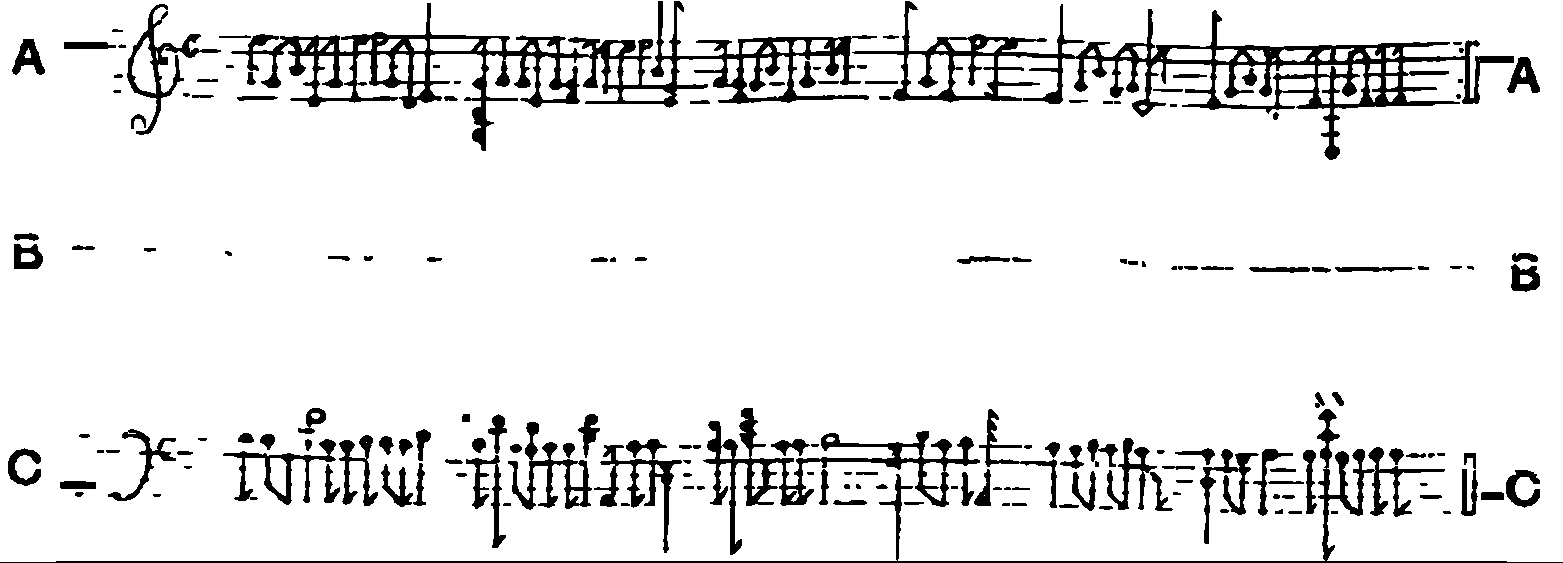
\includegraphics[width=\textwidth]{./images/illus319}}
\label{illus:319}
\end{figure*}
If it be creased along the lines $BB$ and
$CC$ ($CC$ being along the second line of the second score), and
then folded over, with $B$ inside, so that the crease $C$ lies over
the line $A$ (which is the second line of the first score) thus
\PG----File: 319.png------------------------------------------------------
leaving only the top and bottom of the piece of paper
visible, it will be found to read \emph{conceal yourself, your foes
look for you}. I have seen what
purports to be the original, but of
the truth of the anecdote I know
nothing, and the desirability of concealing
himself must have been so
patent that it was hardly necessary
to communicate it by a cryptograph\index
{Cryptographs, Three@\nobreak--- Three types of|)}.

\phantomsection
\addcontentsline{toc}{section}{Ciphers.
 Use of arbitrary symbols unnecessary}\markright{Ciphers}
I proceed next to some of the
more common types of ciphers\index{Ciphers, Four@\nobreak--- Four types of|(}. It
is immaterial whether we invent
characters to denote the various
letters; or whether we employ special
symbols to represent them, such as
the symbol \hbox{(} for \emph{a}, the symbol \hbox{:} for \emph{b},
and so on; or whether we use the
letters in a non-natural sense, such
as the letter \emph{z} for \emph{a}, the letter \emph{y}
for \emph{b}, and so on. The rules for
reading the cipher will be the same
in each case.

In early times it was a common
practice to invent arbitrary symbols
to represent the letters. If the
symbols are invented for the purpose they provoke attention,
hence it would seem that preferably we should use symbols
which are not likely to attract special notice. For instance,
the symbols may be musical notes, in which case the message
would appear as a piece of music. Geometrical figures have
also been used for the same purpose. It is not even necessary
to employ written signs. Natural objects have often been
used, as in a necklace of beads, or a bouquet of flowers,
where the different shaped or coloured beads or different
flowers stand for different letters or words. An even more
subtle form of disguising the cipher is to make the different
\PG----File: 320.png----------------------------------------------------
distances between consecutive knots or beads indicate the
different letters.

Of all such systems we may say that a careful scrutiny
shows that different symbols are being used, and as soon as
the various symbols are distinguished one from the other
no additional complication is introduced, while for practical
purposes they are more trouble to send or receive than those
written in symbols in current use. Accordingly I confine
myself to ciphers written by the use of the current letters
and numerals.

\phantomsection
\addcontentsline{toc}{section}{Ciphers of Four Types}
It is convenient to divide ciphers into four classes. The
first class comprises ciphers in which the same letter or word
is always represented by the same symbol, and this symbol
always represents the same letter or word. The second class
comprises ciphers in which the same letter or word is, in some
or all cases, represented by more than one symbol, and this
symbol always represents the same letter or word. The third
class comprises ciphers in which the same symbol represents
sometimes one letter or word and sometimes another. The
fourth class comprises ciphers in which each letter or word is
always represented by the same symbol, but more than one
letter or word may be represented by the same symbol.

\phantomsection
\addcontentsline{toc}{subsection}{Ciphers of the First Type. Illustrations}
A cipher of the first type then is one in which the same
letter or word is always represented by the same symbol, and
this symbol always represents the same letter or word.

Perhaps the simplest illustration of a cipher of this type
is to employ one language, but written as far as practical in
the alphabet of another language. It is said that during the
Indian Mutiny messages in English, but written in Greek
characters, were used freely, and successfully baffled the
ingenuity of the enemy, into whose hands they fell. If this
is true, the intelligence of the Hindoos must have been much
less than that with which they are usually credited. The
device, however, is an old one, for we are told\footnote
{Sir John Hayward\index{Hayward, J.}, \textit{Life of Edward~VI.},
edition of 1636, p.~20.} that
Edward~VI\index{Edward VI} was accustomed to make notes in cipher ``with
\PG----File: 321.png------------------------------------------------------
Greek characters, to the end that they who waited on him
should not read them.''

A common cipher of this type is made by using the actual
letters of the alphabet, but in a non-natural sense as indicating
other letters. Thus we may use each letter to represent
the one immediately following it in the natural order of the
alphabet---the letters being supposed to be cyclically arranged---\emph{a}
standing for \emph{b} wherever it occurs, \emph{b} standing for \emph{c}, and
so on, and finally \emph{z} standing for \emph{a}. Or more generally we
may write the letters of the alphabet in a line, and under them
re-write the letters in any order we like. For instance
\[
\vbox{\itshape\def\tabcolsep{.25em}\centering
\begin{tabular}{ccccc ccccc ccccc ccccc ccccc c}
a & b & c & d & e & f & g & h & i & j & k & l & m & n & o & p & q & r &
 s & t & u & v & w & x & y & z \\
o & l & k & m & a & z & s & q & x & e & u & f & y & r & t & h & c & w &
 b & v & n & i & d & g & j & p
\end{tabular}}
\]
In such a scheme, we must in our communication replace \emph{a}
by \emph{o}, \emph{b} by \emph{l}, etc. The recipient will prepare a key by
rearranging the letters in the second line in their natural order
and placing under them the corresponding letter in the first
line. Then wherever \emph{a} comes in the message he receives he
will replace it by \emph{e}; similarly he will replace \emph{b} by \emph{s},
and so on.

A cipher of this kind is not uncommonly used in military
signalling, the order of the letters being given by the use of
a key-word. If, for instance, \emph{Pretoria} is chosen as the key-word,
we write the letters in this order, striking out any
which occur more than once, and continue with the unused
letters of the alphabet in their natural order, writing the
whole in two lines thus:
\[
\vbox{\itshape\def\tabcolsep{.25em}\centering
\begin{tabular}{ccccc ccccc ccc}
p & r & e & t & o & i & a & b & c & d & f & g & h \\
z & y & x & w & v & u & s & q & n & m & l & k & j
\end{tabular}}
\]
Then in using the cipher \emph{p} is replaced by \emph{z} and
\textit{vice versâ},
\emph{r} by \emph{y}, and so on. A long message in such a cipher would be
easily discoverable, but it is rapidly composed by the sender
and read by the receiver, and for some purposes may be
useful, especially if the discovery of the purport of the
message is, after a few hours, immaterial.

\PG----File: 322.png------------------------------------------------------
A summary of the usual rules for reading ciphers of this
type, whether written in English, French, German, Italian,
Dutch, Latin, or Greek, was given by D.A.~Conradus\index{Conradus, D.A.} in
1742\footnote
{\textit{Gentleman's Magazine}, 1742, vol.~\textsc{xii}, pp.~133--135,
185--186, 241--242, 473--475. See also the \textit{Collected Works of
E.A.~Poe\index{Poe, E.A.}} in 4 volumes, vol.~\textsc{i}, p.~30 \etseq};
and similar rules have been given by various later
writers. In English the letter which occurs most frequently
is \emph{e}. The next most common letters are said to be \emph{t}, \emph{a},
\emph{o}, and \emph{i}; then \emph{n}; then \emph{r}, \emph{s}, and \emph{h};
then \emph{d} and \emph{l}; then \emph{c}, \emph{w}, \emph{u},
and \emph{m}; then \emph{f}, \emph{y}, \emph{g}, \emph{p}, and \emph{b};
then \emph{v} and \emph{k}; and then \emph{x}, \emph{q}, \emph{j},
and \emph{z}. The most common double letters are \emph{ee}, \emph{ll},
\emph{oo}, and \emph{ss};
while in more than half the cases of a double letter at the end
of a word, the letter is either \emph{l} or \emph{s}. Also, \emph{t} and
\emph{h} form a
common conjunction. I need not, however, go here into further
details of this kind.

Assuming that the division into words is given, that non-significant
symbols are not introduced, and that the problem
is not complicated by the avoidance of the use of common
words, a communication of any considerable length can usually
be read with but little difficulty. The hints given by Conradus
will at once suggest certain hypotheses as to which letters
stand for which. Taking one of these hypotheses we write
the message, replacing the symbols by the letters we conjecture
that they represent and replace the others by dots.
If the hypothesis is tenable, the arrangement will probably
suggest some of the missing letters. If, for example, we find
two words \hbox{emph{s-all}} and \hbox{emph{t-e}} where the missing letter is represented
by the same symbol, the first word shows us that the
missing letter is \emph{h}, \emph{m}, or \emph{t}, and the second word
shews us
that it must be \emph{e}, \emph{h}, \emph{i}, or \emph{o}, hence it must be
\emph{h}. Every fresh
letter so determined makes the hypothesis more probable and
renders it easier to guess what the remaining symbols represent.
The chief difficulty is to get a working hypothesis for
the first few letters---if it is the true solution, probably the
\PG----File: 323.png------------------------------------------------------
puzzle will be readily solved---but to make up a working
hypothesis for even a few letters requires patience.

Ciphers of this class in which the division between the
words is given are to be avoided. If we leave a space
between such words a would-be decipherer is given an immense
help. He will naturally try if a word denoted by a single
symbol can be an \emph{i} or an \emph{a}, while the words of two or three
letters will often stand revealed and so provide a definite
groundwork on which he can construct the key. A long
word may also betray the secret. For instance, if the
decipherer has reason to suspect that the message related to
something connected with Birmingham, and he found that a
particular word of ten letters had its second and fifth letters
alike, as also its fourth and tenth letters, he would naturally see
how the key would work if the word represented Birmingham,
and on this hypothesis would at once know the letters represented
by eight symbols. With reasonable luck this should
suffice to enable him to tell if the hypothesis was tenable.
The effect of this can be avoided by leaving no spaces between
the words, but this might lead to confusion and is not to
be recommended. We can also use letters which occur but
rarely, such as \emph{j}, \emph{q}, \emph{x}, \emph{z}, to separate words,
and probably this is the best method.

Ciphers of this type suggest themselves naturally to those
approaching the subject for the first time, and are commonly
made by merely shifting the letters a certain number of places
forward. If this is done we may decrease the risk of detection
by altering the amount of shifting at short (and preferably
irregular) intervals. Thus it may be agreed that if initially
we shift every letter one place forward then whenever we
come to the letter (say) \emph{n} we shall shift every letter one more
place forward. In this way the cipher changes continually,
and is essentially changed to one of the third class; but even
with this improvement it is probable that an expert would
decode a fairly long message without much difficulty.

We can have ciphers for numerals as well as for letters:
\PG----File: 324.png------------------------------------------------------
such ciphers are common in many shops. Any word or sentence
containing ten different letters will answer the purpose. Thus,
an old tradesman of my acquaintance used the excellent precept
\emph{Be just O Man}---the first letter representing 1, the second $2$,
and so on. In this cipher the price $10$/$6$ would be marked
\emph{bn}/\emph{t}. This is an instance of a cipher of the first type.

\phantomsection
\addcontentsline{toc}{subsection}{Ciphers of the Second Type. Illustrations}
A cipher of the second type is one in which the same
letter or word is, in some or all cases, represented by more
than one symbol, and this symbol always represents the same
letter or word. Such ciphers were uncommon before the
Renaissance, but the fact that to those who held the key they
were not more difficult to write or read than ciphers of the
first type, while the key was not so easily discovered, led
to their common adoption in the seventeenth century.

A simple instance of such a cipher is given by the use of
numerals to denote the letters of the alphabet. Thus \emph{a} may
be represented by $11$ or by $37$ or by $63$, \emph{b} by $12$ or by $38$ or
by $64$, and so on, and finally \emph{z} by $36$ or by $62$ or by $88$, while
we can use $89$ or $90$ to signify the end of a word and the
numbers $91$ to $99$ to denote words or sentences which constantly
occur. Of course in practice no one would employ
the numbers in an order like this, which suggests their
meaning, but it will serve to illustrate the principle. I have
deliberately used numbers of only two digits, as the recipient
can then point off the symbols used in twos, and will know
that each pair of symbols represents a letter, word, or sentence
in the message. A disadvantage of this cipher is that
since each letter is denoted by two symbols the length of the
message is doubled by putting it in cipher.

The cipher can be improved by introducing after every
(say) eleventh digit a non-significant digit. If this is done
the recipient of the message must erase every twelfth digit
before he begins to read the message. With this addition the
difficulty of discovering the key is considerably increased.

The same principle is sometimes applied with letters instead
of numbers. For instance, if we take a word (say) of $n$ letters,
\PG----File: 325.png-----------------------------------------------------
preferably all different, and construct a table as shown below
of $n^2$ cells, each cell is defined by two letters of the key-word.
Thus, if we choose the word \emph{smoking-cap} we shall have $100$
\begin{figure*}[!hbt]
\centering
\makeatletter
\def\Sq@r#1{\vbox to\SqHt{\vss\hbox to\SqWd{\smaller\hss
 \vphantom{yl}#1\hss}\vss}}
\begin{MagicSquare}{11}
{}& {\emph{S}} & {\emph{M}} & {\emph{O}} & {\emph{K}} & {\emph{I}}
 & {\emph{N}} & {\emph{G}} & {\emph{C}} & {\emph{A}} & {\emph{P}} \\
{\emph{S}} & a & b & c & d & e & f & g & h & i & j \\
{\emph{M}} & k & l & m & n & o & p & q & r & s & t \\
{\emph{O}} & u & v & w & x & y & z & a & b & c & d \\
{\emph{K}} & e & f & g & h & i & j & k & l & m & n \\
{\emph{I}} & o & p & q & r & s & t & u & v & w & x \\
{\emph{N}} & y & z & a & b & c & d & e & f & g & h \\
{\emph{G}} & i & j & k & l & m & n & o & p & q & r \\
{\emph{C}} & s & t & u & v & w & x & y & z & {}& {}\\
{\emph{A}} & {}& {}& {}& {}& {}& {}& {}& {}& {}& {}\\
{\emph{P}} & {}& {}& {}& {}& {}& {}& {}& {}& {}& {}\\
\put(1,0){\line(0,1){11}}
\put(0,10){\line(1,0){11}}
\end{MagicSquare}
\end{figure*}
cells, and each cell is determined uniquely by the two letters
denoting its row and column. If we fill these cells in order
with the letters of the alphabet we shall have a system similar
to that explained above, where \emph{a} will be denoted by \emph{ss}
or \emph{og}
or \emph{no}, and so for the other letters. The last $22$ cells may be
used to denote the first $22$ letters of the alphabet, or better,
three or four of them may be used after the end of a word to
show that it is ended, and the rest may be used to denote
words or sentences which are likely to occur frequently.

Like the similar cipher with numbers this can be improved
by introducing after every $m$th letter any single letter which
it is agreed shall be non-significant. To decipher a communication
so written it is necessary to know the clue-word
and the clue-number.

Here for instance is a communication written in the above
cipher with the clue-word \emph{smoking-cap}, and with $7$ as the
clue-number:
{\CryptoSetup
\emph{n\.g\.m\.k\.s\.i\.g\.r\.i\.o\.i\.c\.p\.s\.s\.a\.m\.c\.k\.s\.c\.a\.k%
\.q\.i\.g\.n\.a\.s\.s\.n\.x\.m\.i\.g\.p\.o\.a\.s\.u\.i\.a\.m\.n\.o\.c\.m%
\.p\.a\.m\.i\.n\.s\.c\.n\.o\.g\.c\.p\.n\.c\.i\.s\.y\.i\.k\.s\.k\.a\.m\.s%
\.s\.s\.g\.n\.n%\.n removed to allow deciphering
\.c\.a\.e\.k\.k\.n\.o\.o\.m\.k\.h\.s\.c\.p\.c\.m\.s\.c%
\.b\.g\.p\.n\.g\.s\.i\.a\.%
\PG----File: 326.png------------------------------------------------------
w\.s\.s\.g\.i\.g\.g\.n\.d\.i\.i\.c\.a}}\footnoteT
{The original text read \textellipsis\emph{sssgnnn}\textellipsis, which
leads to gobbledegook in the deciphered message.}.
% Enemy are in force at the ford and have three guns
In this sentence the letters denoting the 79th,
80th, 81st, and 82nd cells have been used to denote the end of
a word, and no use has been made of the last 18 cells.

Another cipher of this type is made as follows\footnote
{The method is well known. It is mentioned by E.A.~Poe\index{Poe, E.A.},
\textit{Collected Works}, vol.~\textsc{iii}, pp.~338--9, but is much older.}.
The sender and recipient of the message furnish themselves with
identical copies of some book. In the cipher only numerals are
used, and these numerals indicate the locality of the letters in
the book. For example, the first letter in the communication
might be indicated by 79--8--5, meaning that it is the 5th letter
in the 8th line of the 79th page. But though secrecy might
be secured, it would be very tedious to prepare or decode a
message, and the method is not as safe as some of those
described below.

Another cipher of this type is for the sender and receiver
to agree on some common book of reference and to agree
further on a number which, if desired, may be communicated
as part of the message. To employ this cipher the page of
the book indicated by the given number must be used. The
first letter in it is taken to signify \emph{a}, the next \emph{b}, and so
on--any letter which occurs a second time or more frequently
being neglected. It may be also arranged that after $n$ letters
of the message have been ciphered, the next $n$ letters shall be
written in a similar cipher taken from the $p$th following page
of the book, and so on. Thus the possession of the code-book
would be of little use to anyone who did not also know the
numbers employed. It is so easy to conceal the clue number
that with ordinary prudence it would be almost impossible for
an unauthorized person to discover a message sent in this
cipher. The clue number may be communicated indirectly in
many ways. For instance, it may be arranged that the
number to be used shall be the number sent, plus (say) $q$, or
that the number to be used shall be an agreed multiple of the
number actually sent.

\PG----File: 327.png------------------------------------------------------
\phantomsection
\addcontentsline{toc}{subsection}{Ciphers of the Third Type. Illustrations}
A cipher of the third type is one in which the same
symbol represents sometimes one letter or word and sometimes
another. Usually such ciphers are easily made or read
by those who have the key, but are difficult to discover by
those who do not possess it.

A simple example is the employment of pre-arranged
numbers in shifting forward the letters that make the communication.
For instance, if we agree on the clue number
(say) $4276$, then the first letter in the communication is
replaced by the fourth letter which follows it in the natural
order of the alphabet: for instance, if it were an \emph{a} it would
be replaced by \emph{e}. The next letter is replaced by the second
letter which follows it in the natural order of the alphabet:
for instance, if it were an \emph{a} it would be replaced by \emph{c}.
The next letter is replaced by the seventh after it. The next by the
sixth after it. The next by the fourth, and so on to the end
of the message. Of course to read the message the recipient
would reverse the process. If the letters of the alphabet are
written at uniform intervals along a ruler, and another ruler
similarly marked with the digits can slide along it, the letter
corresponding to the shifting of any given number of places
can be read at once.

It would be undesirable to allow the division into words
to appear in the message, and either the words must be run
on continuously, or preferably the less common letters \emph{j, q, z}
may be used to mark the division of words. It is also well
to conceal the number of digits in the clue-number. This
can be done and the cipher much improved by inserting after
every (say) $m$th letter a non-significant letter.

Here for instance is a communication written in this
cipher with the clue-numbers $4276$ and $7$:
{\CryptoSetup
\emph{a\.t\.p\.z\.n\.h\.v\.a\.x\.u\.x\.h\.i\.e\.p\.x\.%
a\.f\.w\.g\.h\.z\.n\.i\.y\.p\.r\.p\.s\.i\.k\.b\.d\.k\.z\.y\.y\.g\.k\.q\.%
p\.r\.g\.e\.z\.u\.y\.t\.l\.k\.o\.b\.l\.d\.i\.f\.e\.b\.z\.m\.x\.l\.p\.o\.%
g\.q\.u\.y\.i\.t\.c\.m\.g\.x\.%
k\.c\.k\.u\.e\.x\.v\.s\.q\.k\.a\.z\.i\.a\.g\.g\.s\.i\.g\.a\.y\.t\.n\.v\.%
v\.s\.s\.t\.y\.v\.u\.a\.s\.l\.y\.w\.g\.j\.u\.z\.m\.c\.s\.f\.c\.t\.q\.b\.%
p\.w\.j\.v\.a\.e\.p\.f\.x\.h\.i\.%
b\.w\.p\.x\.i\.u\.l\.t\.x\.l\.a\.v\.v\.t\.q\.z\.o\.x\.w\.k\.v\.t\.u\.v\.%
v\.f\.h\.e\.q\.b\.x\.n\.p\.v\.i\.s\.m\.p\.h\.z\.m\.q\.t\.u\.w\.x\.j\.y\.%
k\.e\.e\.v\.l\.t\.i\.f}}.
% Writ for vacant seat will be issued next week Executive Conservative
% committee meets tomorrow Essential you should be present Opposition
% to your nomination threatened
The recipient would begin by striking out every eighth letter.
He would then shift back every letter 4, 2, 7, 6, 4, 2,~\&c.,
\PG----File: 328.png------------------------------------------------------
places respectively, and in reading it would leave out the
letters \emph{j}, \emph{q}, and \emph{z} as only marking the ends of words.

This is an excellent cipher, and it has the additional merit
of not materially lengthening the message. It can be rendered
still more difficult by arranging that either or both the clue-numbers
shall be changed according to some definite scheme,
and it may be further agreed that they shall change automatically
every day or week.

A somewhat similar system was proposed by Wilkins\index
{Wilkins on Ciphers}\label{page:Wilkins}\footnote
{\textit{Mercury}, by J.~Wilkins, London, 1641, pp.~59, 60.}.
He took a key-word, such as \emph{prudentia}, and constructed as
many alphabets as there were letters in it, each alphabet
being arranged cyclically and beginning respectively with the
letters $p$, $r$, $u$, $d$, $e$, $n$, $t$, $i$, and $a$.
He thus got a table like
the following, giving nine possible letters which might stand
for any letter of the alphabet\Editorial
{Except \emph{j}; perhaps the cipher was intended for use with Latin.}.
Using this we may vary the
\begin{figure*}[!hbt]
\centering
\small\unitlength=1.4em
\makeatletter
\def\Sq@r#1{\vbox to1.4em{\vss\hbox to1.4em{\smaller
  \hss\vphantom{yl}#1\hss}\vss}}
\hspace*{-\textwidth}
\begin{MagicSquare}{25}[10]
  a & b & c & d & e & f & g & h & i & k & l & m & n
    & o & p & q & r & s & t & u & v & w & x & y & z  \\
  p & q & r & s & t & u & v & w & x & y & z & a & b
    & c & d & e & f & g & h & i & k & l & m & n & o  \\
  r & s & t & u & v & w & x & y & z & a & b & c & d
    & e & f & g & h & i & k & l & m & n & o & p & q  \\
  u & v & w & x & y & z & a & b & c & d & e & f & g
    & h & i & k & l & m & n & o & p & q & r & s & t  \\
  d & e & f & g & h & i & k & l & m & n & o & p & q
    & r & s & t & u & v & w & x & y & z & a & b & c  \\
  e & f & g & h & i & k & l & m & n & o & p & q & r
    & s & t & u & v & w & x & y & z & a & b & c & d  \\
  n & o & p & q & r & s & t & u & v & w & x & y & z
    & a & b & c & d & e & f & g & h & i & k & l & m  \\
  t & u & v & w & x & y & z & a & b & c & d & e & f
    & g & h & i & k & l & m & n & o & P & q & r & s  \\
  i & k & l & m & n & o & p & q & r & s & t & u & v
    & w & x & y & z & a & b & c & d & e & f & g & h  \\
  a & b & c & d & e & f & g & h & i & k & l & m & n
    & o & p & q & r & s & t & u & v & w & x & y & z \\
\put(0,9){\line(1,0){25}}
\end{MagicSquare}
\hspace*{-\textwidth}
\end{figure*}
cipher in successive words or letters of the communication.
Thus the message \emph{The prisoners have mutinied and seized the
railway station} would, according as the cipher changes in successive
words or letters, read as \emph{Hwt fhziedvhi bupy pxwmqmhg
erh ervmrq max zirteig station} or as \emph{Hyy svvlwnthm lehx
\PG----File: 329.png----------------------------------------------------
uukzgmiq tvd gvcciq mqe frcoanr atpkcrr}. I have taken
Wilkins's key-word, but it is obvious that it would be desirable
to omit \emph{a} wherever it appears in it, since otherwise, if the
cipher changes in successive words, some of the words may
appear unaltered in the cipher, as is shown in the first of the
examples given above.

\phantomsection
\addcontentsline{toc}{subsection}{Ciphers of the Fourth Type. Illustrations}
A cipher of the fourth type is one in which each letter is
always represented by the same symbol, but more than one
letter may be represented by the same symbol. Such ciphers
were not uncommon at the beginning of the nineteenth century,
and were usually framed by means of a key-sentence containing
about as many letters as there are letters in the alphabet.

Thus if the key-phrase is \emph{The fox jumped over the garden
gate}, we write under it the letters of the alphabet in their
usual sequence as shown below:
\[
\vbox{\itshape\def\tabcolsep{.15em}\centering
\begin{tabular}{cccccccccccccccccccccccccccccccccccc}
T&h&e&~&f&o&x&~&j&u&m&p&e&d&~&o&v&e&r&~&t&h&e&~&g&a&r&d&e&n&~&g&a&t&e&. \\
a&b&c& &d&e&f& &g&h&i&j&k&l& &m&n&o&p& &q&r&s& &t&u&v&w&x&y& &z&a&b&c&. \\
\end{tabular}}
\]
Then we write the message replacing \textit{a} by \textit{t} or \textit{a},
\textit{b} by \textit{h}
or \textit{t}, \textit{c} by \textit{e}, \textit{d} by \textit{f}, and so on.
Here is such a message.
\textit{M foemho nea ge eoo jmdhohg avf teg ev ume afrmeo}.
% I desire you to see Gilbert and act on his advice
But it will
be observed that in the cipher \textit{a} may represent \textit{a} or
\textit{u}, \textit{d} may
represent \textit{l} or \textit{w}, \textit{e} may represent \textit{c} or
\textit{k} or \textit{o} or \textit{s} or \textit{x}, \textit{g} may
represent \textit{t} or \textit{z}, \textit{h} may represent \textit{b} or
\textit{r}, \textit{o} may represent \textit{e} or
\textit{m}, \textit{r} may represent \textit{p} or \textit{v}, and
\textit{t} may represent \textit{a} or \textit{b} or \textit{q}.
And the recipient, in deciphering it, must judge as best he can
which is the right meaning to be assigned to these letters
when they appear.

An instance of a cipher of the fourth type is afforded by a
note sent by the Duchess de~Berri\index{Berri, de}\index
{DeBerri@De Berri} to her adherents in Paris,
in which she employed the key phrase
\[
\vbox{\itshape\def\tabcolsep{.15em}\centering
\begin{tabular}{cccccccccccccccccccccccccc}
l&e&~&g&o&u&v&e&r&n&e&m&e&n&t&~&p&r&o&v&i&s&o&i&r&e.\\
a&b& &c&d&e&f&g&h&i&j&k&l&m&n& &o&p&q&r&s&t&u&v&x&y.
\end{tabular}}
\]
Hence in putting her message into cipher she replaced \textit{a} by
\textit{l},
\textit{b} by \textit{e}, \textit{c} by \textit{g}, and so on. She forgot
however to supply the
\PG----File: 330.png-------------------------------------------------------
key to the recipients of the message, but her friend Berryer
had little difficulty in reading it by the aid of the rules
I have indicated, and thence deduced the key-phrase she
had employed\index{Ciphers, Four@\nobreak--- Four types of|)}.

\phantomsection
\addcontentsline{toc}{section}{Requisites in a good Cipher}
Having considered various classes of cryptographs and
ciphers I may now consider what features we should regard
as important in choosing a cipher intended for practical
use\index{Ciphers, Requisites@\nobreak--- Requisites for good|(}.

In the first place, it is obvious that the means employed
should be such as not to excite suspicion if the communication
falls into unauthorized hands. But this is a counsel of
perfection, and almost impossible to attain.

In the second place, we may say that, under modern
conditions in war, finance, or diplomacy, a cipher may be
useless unless it can be telegraphed or telephoned. If this is
deemed important, it will practically restrict us to the use of
the 26 letters of the alphabet, the 10 numerical symbols for
the digits, to which if we like we may add a few additional
marks such as punctuation stops, brackets,~\&c. The same
condition will require that the message should not be
unduly lengthened by being turned into cipher. Hence
any considerable use of non-significant symbols is to be
deprecated.

In the third place, the key to the cipher should be such
that it can be easily reproduced from memory. For, if the
key is so elaborate that those who use it are obliged to preserve
it in some tangible and accessible form, unauthorized
persons may obtain the power of reading messages. Hence
the key should be reproducible at will. Further, it is desirable
that the key should be of such a character that it (or a change
of it) can be telegraphed or otherwise communicated without
the probability of exciting suspicion.

In the fourth place, a cipher should be capable of change
at short intervals. So that if the reading of one message in
it be discovered subsequent messages may be undecipherable
even though the system used is unaltered.

\PG----File: 331.png------------------------------------------------------
Lastly, no ambiguity should be possible in deciphering
the communication. This will exclude ciphers of the fourth
type.

Accordingly in choosing a good cipher we should seek for
one in which only current letters, symbols, or words are
employed; such that its use does not unduly lengthen the
message; such that the key to it can be reproduced at will
and need not be kept in a form which might betray the secret
to an unauthorized person; such that the key to it changes
or can be changed at short intervals; and such that it is not
ambiguous. Many ciphers of the second and third types
fulfil these conditions, but it is generally desirable to avoid
ciphers of the first type unless circumstances permit of the
free use of a code-book\index{Ciphers, Requisites@\nobreak--- Requisites for good|)}.

\phantomsection
\addcontentsline{toc}{section}{Cipher Machines}
The use of instruments giving a cipher, which is or can be
varied constantly and automatically, has been often recommended.
Several have been constructed on the lines of the
well-known letter-locks\footnote
{See, for instance, the descriptions of those devised by Sir Charles
Wheatstone\index{Wheatstone on Ciphers}, given in his \textit
{Scientific Papers}, London, 1879, pp.~342--347;
and by Capt.\ Bazeries in \textit{Comptes Rendus, Association Français
pour l'avancement des sciences}, vol.~\textsc{xx} (Marseilles), 1891,
p.~160, \etseq}. The possession of the key of the
instrument as well as a knowledge of the clue-word is
necessary to enable anyone to read a message, but the risk of
some instrument, when set, falling into unauthorized hands
must be taken into account. Since equally good ciphers can
be constructed without the use of mechanical devices I do not
think their employment can be recommended.

\phantomsection
\addcontentsline{toc}{section}{Historical Ciphers}
This chapter has already run to such a length that I
cannot find space to describe more than one or two ciphers
that appear in history or fiction\index
{Ciphers, Historical@\nobreak--- Historical|(}, but, we may say that
until recently most of the historical ciphers are not difficult
to read.

\phantomsection
\addcontentsline{toc}{subsection}{Julius Caesar, Augustus}
It is said that Julius Caesar\index{Caesar, Julius}\index{Julius Caesar}
in making secret memoranda
was accustomed to move every letter four places forward,
\PG----File: 332.png------------------------------------------------------
writing \emph{d} for \emph{a}, \emph{e} for \emph{b},~\&c. This would be a
very easy
instance of a cipher of the first type, but it may have been
effective at that time. His nephew Augustus\index{Augustus} sometimes used
a similar cipher, in which each letter was moved forward one
place\footnote
{Of some of Caesar's correspondence, Suetonius\index{Suetonius} says
(cap.~56) \emph{si
quis investigare et persequi velit, quartam elementorum literam, id est,
d pro a, et perinde reliquas commutet.} And of Augustus he says (cap.~88)
\emph{quoties autem per notas scribit, b pro a, c pro b, ac deinceps eadem
ratione, sequentes literas ponit; pro x autem duplex a.}}.

\phantomsection
\addcontentsline{toc}{subsection}{Bacon}
Bacon\index{Bacon, Francis} proposed a cipher in which each letter was
denoted
by a group of five letters consisting of \emph{A} and \emph{B} only. Since
there are 32 such groups, he had 6 symbols to spare, which
he could use to separate words or to which he could assign
special meanings. A message in this cipher would be five
times as long as the original message. This may be compared
with the far superior system of the five (or four) digit codebook
system in use at the present time.

\phantomsection
\addcontentsline{toc}{subsection}{Charles I}
Charles~I\index{Charles I|(} used ciphers freely in important
correspondence---the
majority being of the second type. He was foolish
enough to take a cabinet containing many confidential letters
in cipher, to some of which their readings were appended,
on the field of Naseby, where they fell into the hands of
Fairfax\footnote
{\textit{First Report of the Royal Commission on Historical Manuscripts},
1870, pp.~2, 4.}. The House of Commons sent them to a committee
presided over by a Mr~Tate\index{Tate}. It is commonly believed that the
Committee referred the papers to J.~Wallis\index{Wallis, J.}\footnote
{See his letters on Cryptography, \textit{Opera}, vol.~\textsc{iii},
pp.~659--672.}, then Fellow
of Queens' College, Cambridge, and subsequently Savilian
Professor at Oxford, who discovered the key to them. At
any rate the letters were read.

In these ciphers each letter was represented by a number.
The clues to some of the ciphers were provided by the King
who had written over the number the letter which it represented,
as shown in the following quotation:
\PG----File: 333.png----------------------------------------------------
\[
\vbox{\itshape\def\tabcolsep{.3em}\centering
\begin{tabular}{cccccccccccccccccc}
&c&a&t&o&l&i&c&k&s&i&n&F\\
&$11$&$18$&$45$&$35$&$23$&$27$&$11$&$25$&$47$&$28$&$40$&$148$&
 \multicolumn{4}{l}{\upshape haue layed}\\[6pt]
t&h&i&r&p&u&r&s&e&s&t&o&g&e&t&h&e&r\\
$45$&$31$&$27$&$51$&$33$&$62$&$50$&$47$&$7$&$48$&$45$&$35$&$21$&
 $7$&$46$&$32$&$7$&$51$\\[6pt]
f&o&r&&s&u&p&l&y&of&a&r&m&e&s.&--&--&--\\
$15$&$35$&$50$&a&$47$&$62$&$33$&$23$&$74$&k$1$&$17$&$51$&$42$&$7$&
 $47$.&--&--&--
\end{tabular}}
\]

The published letters show that the King used different
ciphers at different times, though perhaps he used the same
one in all correspondence with any particular person, but the
general character of those he employed is the same. The
sentence quoted above is taken from a letter from Queen
Henrietta Maria\index{Henrietta Maria} of January~26, 1643. In this and
another
letter a few months later \textit{a} is represented by 17 or 18,
\textit{b} by 13,
\textit{c} by 11 or 12, \textit{d} by 5, \textit{e} by 7 or 8 or 9 or 10,
\textit{f} by 15 or 16,
\textit{g} by 21, \textit{h} by 31 or 32, \textit{i} by 27 or 28,
\textit{k} by 25, \textit{l} by 23 or 24,
\textit{m} by 42 or 44, \textit{n} by 39 or 40 or 41,
\textit{o} by 35 or 36 or 37 or 38,
\textit{p} by 33 or 34, \textit{r} by 50 or 51 or 52,
\textit{s} by 47 or 48, \textit{t} by 45 or
46, \textit{u} by 62 or 63, \textit{w} by 58, and \textit{y} by 74 or 77.
Numbers of
three digits were used to represent particular people or places.
Thus 148 stood for \emph{France}, 189 for the \emph{King}, 260 for the
\emph{Queen}, 354 for \emph{Prince Rupert}, and so on. Further, there
were a few special symbols, thus \textit{k}$1$ stood for \emph{but}\Editorial
{Or maybe \emph{of}, as in the preceding example.},
\textit{n}$1$ for \emph{to}, and
\textit{f}$1$ for \emph{is}. The numbers 2 to 4 and 65 to 72 were
non-significant,
and were to be struck out or neglected by the recipient
of the message. Each symbol is separated from that which
follows it by a full-stop.

The Queen seems to have found writing in cipher a great
trouble. In the letter from which I have already quoted a
sentence she says \textellipsis\ \emph{que je suis extrement tourmantee du
mal de teete qui fait que je mesteray en syfre par un autre se qui
jovois fait moy mesme}, and she uses the cipher only for the
particular words it was desired to conceal. Thus she writes
\emph{Mr Capell nous a fait voir que sy} 27, 23,~\&c.,~\&c. If by this
she saved herself trouble, she did it at the cost of rendering
the cipher much easier to read.

\PG----File: 334.png------------------------------------------------------
The system used by Charles was in considerable repute
during the seventeenth century, but even without extraneous
help it is possible for a diligent student to discover the key
if the message is fairly long. An excellent illustration of this
fact is to be found in the writings of the late Sir Charles
Wheatstone\index{Wheatstone on Ciphers}. A paper in cipher, every page
of which was
initialled by Charles~I, and countersigned by Lord Digby\index{Digby, Lord},
was purchased some years ago by the British Museum. It
was believed to be a state paper of importance. It consists
of a series of numbers (about 150 different symbols being used)
without any clue to their meaning, or any indication of a
division between the words employed. The task of reading
it was rendered the more difficult by the supposition, which
proved incorrect, that the document was in English; but
notwithstanding this, Sir Charles Wheatstone\index{Wheatstone on Ciphers}
discovered the key\footnote
{The document, its translation, and the key used are given in
Wheatstone's \textit{Scientific Papers}, London, 1879, pp. 321--341.}.
In this cipher \emph{a} was represented by any of the numbers
$12$, $13$, $14$, $15$, $16$, or $17$, \emph{b} by $18$ or $19$, and so on,
while some
$65$ special words were represented by particular numbers.

I may note in passing that Charles also used a species of
shorthand, in which the letters were represented by four
strokes varying in length and position. Essentially the system
is simple, though it is troublesome to read or write\index{Charles I|)}.

\phantomsection
\addcontentsline{toc}{subsection}{Pepys}
The famous diary of Samuel Pepys\index{Pepys, S.|(} is commonly said to
have been written in cipher, but in reality it is written in
shorthand according to a system invented by T.~Shelton\index
{Shelton, T.}\footnote
{\textit{Tachy-graphy} by T.~Shelton. The earliest edition I have seen is
dated 1641. A somewhat similar system by W.~Cartwright\index{Cartwright, W.}
was issued by J.~Rich\index{Rich, J.} under the title \textit{Semographie},
London, 1644.}.
It is however somewhat difficult to read, for the vowels are
usually omitted, and Pepys used some arbitrary signs for
terminations, particles, and certain words---so far turning it
into a cipher. Further, in certain places, when the matter is
such that it can hardly be expressed with decency, he changed
\PG----File: 335.png------------------------------------------------------
from English to a foreign language, or inserted non-significant
letters. Shelton's\index{Shelton, T.} system had been forgotten when
attention was first attracted to the diary. Accordingly we may say
that, to those who first tried to read it, it was written in
cipher, but Pepys's contemporaries would have properly described
it as being written in shorthand, though with a few
modifications of his own invention\index{Pepys, S.|)}.

A system of shorthand specially invented for the purpose
is a true cipher. One such system in which each letter is
represented either by a dot or by a line of constant length
was used by the Earl of Glamorgan\index{Glamorgan, Earl of}, better known
by his subsequent title as Marquis of Worcester\index{Worcester, Marquis of},
in 1645, as also by
Charles~I\index{Charles I}. in some of his private correspondence. It is a
cipher of the first type and has the defects inherent in almost
every cipher of this kind: in fact Glamorgan's letter was
deciphered, and the system discovered by Mr~Dircks\index
{Dircks, H.}\footnote
{\textit{Life of the Marquis of Worcester} by H.~Dircks, London, 1865.
Worcester's system of shorthand was described by him in his \textit
{Century of Inventions}, London, 1663, sections 3, 4, 5.}.
Obsolete systems of shorthand\footnote
{Various systems, including those used in classical and medieval
times, are described in the \textit{History of Shorthand} by
T.~Anderson\index{Anderson, T.}, London, 1882.} might be thus used to form
an effective cipher.

\phantomsection
\addcontentsline{toc}{subsection}{De Rohan}
It is always difficult to read a very short message in
cipher, since necessarily the clues are few in number. When
the Chevalier de~Rohan\index{DeRohan@De Rohan} was sent to the Bastille,
on suspicion
of treason, there was no evidence against him except what
might be extracted from Monsieur Latruaumont\index{Latruaumont}. The latter
died without making any admission. De~Rohan's friends had
arranged with him to communicate the result of Latruaumont's
examination, and accordingly in sending him some fresh body
linen they wrote on one of the shirts \emph{Mg dulhxcclgu ghj yxuj,
lm ct ulgc alj}.
% Le prisonnier est mort, il na rien dit
For twenty-four hours de~Rohan pored over the
message, but, failing to read it, he admitted his guilt, and was
executed November~27, 1674.

\PG----File: 336.png------------------------------------------------------
The cipher is a very simple one of the first type, but the
communication is so short that unless the key were known it
would not be easy to read it. Had de~Rohan suspected that
the second word was \emph{prisonnier}, it would have given him 7
out of the 12 letters used, and as the first and third words
suggest the symbols used for \emph{l} and \emph{t}, he could hardly have
failed to read the message.

\phantomsection
\addcontentsline{toc}{subsection}{Marie Antoinette}
The \vpageref[following cipher][cipher ]{Antoinette} is said to have been
employed by Marie Antoinette\index{Marie Antoinette}\footnote
{The key is given, but without explanation, in \textit{Juniper Hall}, by
C.~Hill\index{Hill, C.}, London, 1904, p.~13.}.
I take it that it was used in the method
\ifPaper\begin{figure*}[!hbt]
\else\begin{figure*}[p]\relsize{-2}\fi
\itshape\centering
\ifPaper
  \def\SqHt{3em}
  \def\SqWd{1.5em}
  \unitlength=1.5em
\else % we have to squeeze a bit tighter
  \def\SqHt{2.8em}
  \def\SqWd{1.4em}
  \unitlength=1.4em\fi
\def\BigSqr#1{\vbox to\SqHt{\vss\setbox0=\hbox to\SqHt
  {\relsize{2}\hss\vphantom{1}#1\/\hss}\dp0=0pt\box0\vss}}
\def\BigCell(#1,#2;#3){\put(#1,#2){\framebox{\BigSqr{#3}}}}
\def\Sqr#1#2{\vbox to\SqHt{\vss\vss\setbox0=\hbox to\SqWd
  {\smaller\hss\vphantom{1}#1\/\hss}\dp0=0pt\box0%
  \setbox0=\hbox to\SqWd{\smaller\hss\vphantom{1}#2\/\hss
  }\dp0=0pt\box0\vss\vss}}
\def\Cell(#1,#2;#3#4){\put(#1,#2){\framebox{\Sqr{#3}{#4}}}}
\begin{picture}(13,22)
\BigCell(0,20;AB)\Cell(2,20;AO)\Cell(3,20;BP)\Cell(4,20;CQ)
  \Cell(5,20;DR)\Cell(6,20;ES)\Cell(7,20;FT)\Cell(8,20;GV)
  \Cell(9,20;HX)\Cell(10,20;IY)\Cell(11,20;LZ)\Cell(12,20;MN)
\BigCell(0,18;CD)\Cell(2,18;MZ)\Cell(3,18;AN)\Cell(4,18;BO)
  \Cell(5,18;CP)\Cell(6,18;DQ)\Cell(7,18;ER)\Cell(8,18;FS)
  \Cell(9,18;GT)\Cell(10,18;HV)\Cell(11,18;IX)\Cell(12,18;LY)
\BigCell(0,16;EF)\Cell(2,16;LN)\Cell(3,16;MO)\Cell(4,16;AP)
  \Cell(5,16;BQ)\Cell(6,16;CR)\Cell(7,16;DS)\Cell(8,16;ET)
  \Cell(9,16;FV)\Cell(10,16;GX)\Cell(11,16;HY)\Cell(12,16;IZ)
\BigCell(0,14;GH)\Cell(2,14;IN)\Cell(3,14;LO)\Cell(4,14;MP)
  \Cell(5,14;AQ)\Cell(6,14;BR)\Cell(7,14;CS)\Cell(8,14;DT)
  \Cell(9,14;EV)\Cell(10,14;FX)\Cell(11,14;GY)\Cell(12,14;HZ)
\BigCell(0,12;IL)\Cell(2,12;HN)\Cell(3,12;IO)\Cell(4,12;LP)
  \Cell(5,12;MQ)\Cell(6,12;AR)\Cell(7,12;BS)\Cell(8,12;CT)
  \Cell(9,12;DV)\Cell(10,12;EX)\Cell(11,12;FY)\Cell(12,12;GZ)
\BigCell(0,10;MN)\Cell(2,10;GN)\Cell(3,10;HO)\Cell(4,10;IP)
  \Cell(5,10;LQ)\Cell(6,10;MR)\Cell(7,10;AS)\Cell(8,10;BT)
  \Cell(9,10;CV)\Cell(10,10;DX)\Cell(11,10;EY)\Cell(12,10;FZ)
\BigCell(0,8;OP)\Cell(2,8;FN)\Cell(3,8;GO)\Cell(4,8;HP)
  \Cell(5,8;IQ)\Cell(6,8;LR)\Cell(7,8;MS)\Cell(8,8;AT)
  \Cell(9,8;BV)\Cell(10,8;CX)\Cell(11,8;DY)\Cell(12,8;EZ)
\BigCell(0,6;QR)\Cell(2,6;EN)\Cell(3,6;FO)\Cell(4,6;GP)
  \Cell(5,6;HQ)\Cell(6,6;IR)\Cell(7,6;LS)\Cell(8,6;MT)
  \Cell(9,6;AV)\Cell(10,6;BX)\Cell(11,6;CY)\Cell(12,6;DZ)
\BigCell(0,4;ST)\Cell(2,4;DN)\Cell(3,4;EO)\Cell(4,4;FP)
  \Cell(5,4;GQ)\Cell(6,4;HR)\Cell(7,4;IS)\Cell(8,4;LT)
  \Cell(9,4;MV)\Cell(10,4;AX)\Cell(11,4;BY)\Cell(12,4;CZ)
\BigCell(0,2;VX)\Cell(2,2;CN)\Cell(3,2;DO)\Cell(4,2;EP)
  \Cell(5,2;FQ)\Cell(6,2;GR)\Cell(7,2;HS)\Cell(8,2;IT)
  \Cell(9,2;LV)\Cell(10,2;MX)\Cell(11,2;AY)\Cell(12,2;BZ)
\BigCell(0,0;YZ)\Cell(2,0;BN)\Cell(3,0;CO)\Cell(4,0;DP)
  \Cell(5,0;EQ)\Cell(6,0;FR)\Cell(7,0;GS)\Cell(8,0;HT)
  \Cell(9,0;IV)\Cell(10,0;LX)\Cell(11,0;MY)\Cell(12,0;AZ)
\put(0,0){\line(0,1){22}}
\put(0,0){\line(1,0){13}}
\put(13,0){\line(0,1){22}}
\put(0,22){\line(1,0){13}}
\end{picture}
\label{Antoinette}
\end{figure*}
\PG----File: 337.png------------------------------------------------------
indicated on page \pageref{page:Wilkins} above. If so, the first word in the
communication would be rewritten according to the scheme
given in the first line, \emph{a} being replaced by \emph{o}, and
\emph{vice versâ},
\emph{b} by \emph{p}, and so on. The second word would be rewritten
according to the scheme in the second line, and so on.

\phantomsection
\addcontentsline{toc}{subsection}{The Code Dictionary}
One of the modern systems is the five digit code-book
cipher\index{Code-Book Ciphers}, to which I have already alluded.
According to the
general belief, it is frequently employed in certain official
communications at the present day. A code dictionary is
prepared in which every word likely to be used is printed,
and the words are numbered consecutively $00000$, $00001, \ldots$
up, if necessary, to $99999$. Thus each word is represented
% removed obvious misprint comma after "if"
by a number of five digits, and there are $10^5$ such
numbers available. The message is first written down in
words. Below that it is written in numbers, each word being
replaced by the number corresponding to it. To each of these
numbers is added some definite prearranged clue-number---the
words in the dictionary being assumed to be arranged
cyclically, so that if the resulting number exceeds $10^5$ it is
denoted only by the excess above $10^5$. The resulting numbers
are sent as a message. On receipt of a message it is divided
into consecutive groups of five numbers, each group representing
a word. From each number is subtracted the prearranged
clue-number, and then the message can be read off by the
code dictionary. When a code message is published by the
Government receiving it, the construction of the sentences is
usually altered before publication, so that the key may not be
discoverable by anyone in possession of the code-book or who
has seen the cipher message. This is a rule applicable to all
cryptographs and ciphers.

This is a cipher with $10^5$ symbols, and as each symbol
consists of five digits, a message of $n$ words is denoted by $5n$
digits, and probably is not longer than the message when
written in the ordinary way. Since however the number of
words required is less than $10^5$, the spare numbers may be
used to represent collocations of words which constantly occur,
and if so the cipher message may be slightly shortened.

\PG----File: 338.png------------------------------------------------------
If the clue number is the same all through the message
it would be possible by not more than $10^5$ trials to discover
the message. This is not a serious risk, but, slight though it
is, it can be avoided if the clue number is varied; the clue
number might, for instance, be $781$ for the first three words,
$791$ for the next five words, $801$ for the next seven words,
and so on. Further it may be arranged that the clue numbers
shall be changed every day; thus on the seventh day of the
month they might be $781$, $791$,~\&c., and on the eighth day
$881$, $891$,~\&c., and so on.

This cipher can however be further improved by inserting
at some step, say after each $m$th digit, an unmeaning digit.
For example, if, in the original message written in numbers, we
insert a $9$ after every seven digits we shall get a collection of
words (each represented by five digits), most of which would
have no connection with the original message, and probably
the number of digits used in the message itself would no
longer be a multiple of $5$. Of course the receiver has only to
reverse the process in order to read the message.

It is however unnecessary to use five symbols for each
word. For if we make a similar code with the twenty-six
letters of the alphabet instead of the ten digits, four letters
for each word or phrase would give us $26^4$, that is, $456976$
possible variations. Thus the message would be shorter and
the power of the code increased. Further, if we like to use
the ten digits and the twenty-six letters of the alphabet---all
of which are easily telegraphed---we could, by only using
three symbols, obtain $36^3$, that is, $46656$ possible words, which
would be sufficient for all practical purposes.

This code, at any rate with these modifications, is undecipherable
by strangers, but it has the disadvantages that those
who use it must always have the code dictionary available,
and that it takes a considerable time to code or decode
a communication. For practical purposes its use would be
confined to communications which could be deciphered at
leisure in an office, It is especially suitable in the case of
\PG----File: 339.png------------------------------------------------------
communications between officials, each supplied with a competent
staff of secretaries or clerks---as from an ambassador
to his chief, or a commander in the field to his war office.
It is an excellent example of a cipher of the first type, but it
is not clear that it possesses any superiority over some of the
simple ciphers of the third type.

\phantomsection
\addcontentsline{toc}{subsection}{Poe's Writings}
One of the best known writers on the subject of cryptographs
and ciphers is E.A.~Poe\index{Poe, E.A.}, indeed probably a good
many readers have made their first acquaintance with a
cipher in his story of \textit{The Gold Bug}, the interest of which
turns on reading a simple cipher of the first type. In earlier
times J.~Tritheim\index{Tritheim, J.} of Spanheim,
G.~Porta\index{Porta, G.} of Naples, Cardan\index{Cardan},
Niceron\index{Niceron}, and J.~Wilkins\index{Wilkins on Ciphers}
occupied much the same position,
while whenever ciphers were freely used skilful decipherers
seem to have arisen.\ifPaper\enlargethispage{12pt}\fi

Poe\index{Poe, E.A.} wrote an essay on cryptography in which he said
that it may be roundly asserted that human ingenuity cannot
concoct a cipher which human ingenuity cannot resolve---a
conclusion which is hardly justified by the known facts. In
an earlier article he once made a similar remark so far as
ciphers of the first class are concerned, with the implied
limitation that only $26$ symbols may be used. In this sense
the observation is correct. His assertion excited some attention,
and numerous communications in cipher were sent to
him. More than one of his correspondents did not play the
game fairly, not only employing foreign languages, but using
several different ciphers in the same communication. Nevertheless
he resolved all except one; and he proved that this
last was a fraud, being merely a jargon of random characters,
having no meaning whatever\index{Ciphers, Historical@\nobreak--- Historical|)}.

\PG----File: 340.png------------------------------------------------------
% CHAPTER XII
\chapter[Hyper-space.]{Hyper-space\protect\footnotemark.}

\textsc{I propose} to devote the remaining pages to the
consideration\chapindex{Hyper-space@\textsc{Hyper-space}}%
\chapindex{Geometry, Non-Euclidean@\textsc{Geometry, Non-Euclidean}}%
\chapindex{Space@\textsc{Space}, Properties of},
from the point of view of a mathematician, of certain
properties of space, time, and matter, and to a sketch of some
hypotheses as to their nature. I shall not discuss the metaphysical\footnotetext
{% we put this below the first few lines to force
% some text on the page under the heading!
On the possibility of the existence of space of more than three
dimensions see C.H.~Hinton\index{Hinton on Space}, \textit
{Scientific Romances}, London, 1886, a most
interesting work, from which I have derived much assistance in compiling
the earlier part of this chapter; his later work, \textit
{The Fourth Dimension},
London, 1904, may be also consulted. See also G.F.~Rodwell\index
{Rodwell on Hyper-space}, \textit{Nature},
May~1, 1873, vol.~\textsc{viii}, pp.~8, 9; and E.A.~Abbott\index
{Abbott, E.A.}, \textit{Flatland}, London, 1884.
\endgraf
The theory of Non-Euclidean geometry is due primarily to
Lobatschewsky\index{Lobatschewsky, N.I.},
\textit{Geometrische Untersuchungen zur Theorie der Parallellinien},
Berlin, 1840 (originally given in a lecture in 1826); to Gauss\index{Gauss}
(\Eg\ letters to Schumacher, May~17, 1831, July~12, 1831, and Nov.~28, 1846,
printed in Gauss's collected works); and to J.~Bolyai, Appendix to the
first volume of his father's \textit{Tentamen}, Maros-Vásárkely, 1832;
though the subject had been discussed by J.~Saccheri\index{Saccheri, J.}
as long ago as 1733: its development was mainly the work of
G.F.B.~Riemann\index{Riemann, G.F.B.}, \textit{Ueber die Hypothesen
welche der Geometrie zu Grunde liegen}, written in 1854, \textit
{Göttinger Abhandlungen}, 1866--7, vol.~\textsc{xiii}, pp.~131--152
(translated in \textit{Nature}, May~1 and 8, 1873, vol.~\textsc{viii},
pp.~14--17, 36--37); H.L.F.~von Helmholtz\index{Helmholtz}\index
{Von Helmholz}, \textit{Göttinger Nachrichten}, June~3, 1868,
pp.~193--221; and E.~Beltrami\index{Beltrami on Space}, \textit{Saggio di
Interpretazione della Geometria non-Euclidea}, Naples, 1868, and the
\textit{Annali di Matematica}, series~2, vol.~\textsc{ii}, pp.~232--255:
see an article by von Helmholtz in the \textit{Academy}, Feb.~12, 1870,
vol.~\textsc{i}, pp.~128--131. Within the last
twenty-five years the theory has been treated by several mathematicians.
\endgraf
A bibliography of hyper-space, compiled by G.B.~Halsted\index
{Halsted on Hyper-space}, appeared in the \textit{American Journal of
Mathematics}, vol.~\textsc{i} (1878), pp.~261--276,
384--385; and vol.~\textsc{ii} (1879), pp.~65--70.}
\PG----File: 341.png---------------------------------------------------------
theories that profess to account for the origin of our
conceptions of them, for these theories lead to no practical
result and rest on assertions which are incapable of definite
proof---a foundation which does not commend itself to a scientific
student. Space, time, and matter cannot be defined; but
the means of measuring them and the investigation of their
properties fall within the domain of mathematics.

I devote this chapter to considerations connected with
space, leaving the subjects of time and mass to the following
two chapters.

\phantomsection
\addcontentsline{toc}{section}{Two subjects of speculation on Hyper-space}
I shall confine my remarks on the properties of space to
two speculations which recently have attracted considerable
attention. These are (i)~the possibility of the existence of
space of more than three dimensions, and (ii)~the possibility
of kinds of geometry, especially of two dimensions, other than
those which are treated in the usual text-books. These problems
are related. The term hyper-space was used originally
of space of more than three dimensions, but now it is often
employed to denote also any Non-Euclidean space. I attach
the wider meaning to it, and it is in that sense that this
chapter is on the subject of hyper-space.

\phantomsection
\addcontentsline{toc}{section}{Space of two dimensions and of one dimension}
In regard to the first of these questions, the conception of
a world of more than three dimensions is facilitated by the fact
that there is no difficulty in imagining a world confined to only
two dimensions---which we may take for simplicity to be a
plane, though equally well it might be a spherical or other surface.
We may picture the inhabitants of flatland\index{Flat-land|(} as moving
either on the surface of a plane or between two parallel and
adjacent planes. They could move in any direction along the
plane, but they could not move perpendicularly to it, and
would have no consciousness that such a motion was possible.
We may suppose them to have no thickness, in which case
they would be mere geometrical abstractions: or, preferably,
we may think of them as having a small but uniform thickness,
in which case they would be realities.

\PG----File: 342.png---------------------------------------------------------
Several writers have amused themselves by expounding and
illustrating the conditions of life in such a world. To take a
very simple instance, in flatland---or any even dimensional
space---a knot is impossible, a simple alteration which alone
would make some difference in the experience of the inhabitants
as compared with our own.

If an inhabitant of flatland was able to move in three
dimensions, he would be credited with supernatural powers by
those who were unable so to move; for he could appear or
disappear at will, could (so far as they could tell) create matter
or destroy it, and would be free from so many constraints to
which the other inhabitants were subject that his actions
would be inexplicable by them.

We may go one step lower, and conceive of a world of one
dimension---like a long tube---in which the inhabitants could
move only forwards and backwards. In such a universe there
would be lines of varying lengths, but there could be no
geometrical figures. To those who are familiar with space of
higher dimensions, life in line-land\index{Line-land} would seem somewhat
dull. It is commonly said that an inhabitant could know only two
other individuals; namely, his neighbours, one on each side.
If the tube in which he lived was itself of only one dimension,
this is true; but we can conceive an arrangement of tubes in
two or three dimensions, where an occupant would be conscious
of motion in only one dimension, and yet which would permit
of more variety in the number of his acquaintances and conditions
of existence.

\phantomsection
\addcontentsline{toc}{section}{Space of four dimensions}
Our conscious life is in three dimensions, and naturally the
idea occurs whether there may not be a fourth dimension. No
inhabitant of flatland could realize what life in three dimensions
would mean, though, if he evolved an analytical geometry
applicable to the world in which he lived, he might be able to
extend it so as to obtain results true of that world in three
dimensions which would be to him unknown and inconceivable.
Similarly we cannot realize what life in four dimensions
is like, though we can use analytical geometry to obtain results
\PG----File: 343.png---------------------------------------------------------
true of that world, or even of worlds of higher dimensions.
Moreover the analogy of our position to the inhabitants of flatland
enables us to form some idea of how inhabitants of space
of four dimensions would regard us.

\phantomsection
\addcontentsline{toc}{subsection}{Existence in such a world}
Just as the inhabitants of flatland might be conceived as
being either mere geometrical abstractions, or real and of a
uniform thickness in the third dimension, so, if there is a fourth
dimension, we may be regarded either as having no thickness
in that dimension, in which event we are mere (geometrical)
abstractions---as indeed idealist philosophers have asserted to
be the case---or as having a uniform thickness in that dimension,
in which event we are living in four dimensions although
we are not conscious of it. In the latter case it is reasonable
to suppose that the thickness in the fourth dimension of bodies
in our world is small and possibly constant; it has been conjectured
also that it is comparable with the other dimensions
of the molecules of matter, and if so it is possible that the constitution
of matter and its fundamental properties may supply
experimental data which will give a physical basis for proving
or disproving the existence of this fourth dimension.

If we could look down on the inhabitants of flatland we
could see their anatomy and what was happening inside them.
Similarly an inhabitant of four-dimensional space could see
inside us.

An inhabitant of flatland could get out of a room, such as a
rectangle, only through some opening, but, if for a moment he
could step into three dimensions, he could reappear on the other
side of any boundaries placed to retain him. Similarly, if we
came across persons who could move out of a closed prison-cell
without going through any of the openings in it, there might
be some reason for thinking that they did it by passing first
in the direction of the fourth dimension and then back again
into our space. This however is unknown.

Again, if a finite solid was passed slowly through flatland,
the inhabitants would be conscious only of that part of it
which was in their plane. Thus they would see the shape of
\PG----File: 344.png---------------------------------------------------------
the object gradually change and ultimately vanish. In the
same way, if a body of four dimensions was passed through our
space, we should be conscious of it only as a solid body, namely,
the section of the body by our space, whose form and appearance
gradually changed and perhaps ultimately vanished. It
has been suggested that the birth, growth, life, and death of
animals may be explained thus as the passage of finite four-dimensional
bodies through our three-dimensional space. I
believe that this idea is due to Mr~Hinton\index{Hinton on Space}.

The same argument is applicable to all material bodies.
The impenetrability and inertia of matter are necessary consequences;
the conservation of energy follows, provided that the
velocity with which the bodies move in the fourth dimension
is properly chosen: but the indestructibility of matter rests on
the assumption that the body does not pass completely through
our space. I omit the details connected with change of density
as the size of the section by our space varies.

\phantomsection
\addcontentsline{toc}{subsection}{Arguments in favour of the existence
of such a world}
We cannot prove the existence of space of four dimensions,
but it is interesting to enquire whether it is probable that
such space actually exists. To discuss this, first let us consider
how an inhabitant of flatland might find arguments to support
the view that space of three dimensions existed, and then
let us see whether analogous arguments apply to our world.
I commence with considerations based on geometry and then
proceed to those founded on physics.

Inhabitants of flatland would find that they could have two
triangles of which the elements were equal, element to element,
and yet which could not be superposed. We know that the
explanation of this fact is that, in order to superpose them, one
of the triangles would have to be turned over so that its undersurface
came on to the upper side, but of course such a movement
would be to them inconceivable. Possibly however they
might have suspected it by noticing that inhabitants of one-dimensional
space might experience a similar difficulty in
comparing the equality of two lines, $ABC$ and $CB'A'$, each
defined by a set of three points. We may suppose that the
\PG----File: 345.png---------------------------------------------------------
lines are equal and such that corresponding points in them
could be superposed by rotation round $C$---a movement
inconceivable to the inhabitants---but an inhabitant of such
a world in moving along from $A$ to $A'$ would not arrive at the
corresponding points in the two lines in the same relative
order, and thus might hesitate to believe that they were
equal. Hence inhabitants of flatland might infer by analogy
that by turning one of the triangles over through three-dimensional
space they could make them coincide.

We have a somewhat similar difficulty in our geometry.
We can construct triangles in three dimensions---such as two
spherical triangles---whose elements are equal respectively one
to the other, but which cannot be superposed. Similarly we
may have two spirals whose elements are equal respectively,
one having a right-handed twist and the other a left-handed
twist, but it is impossible to make one fill exactly the same
parts of space as the other does. Again, we may conceive of
two solids, such as a right hand and a left hand, which are
exactly similar and equal but of which one cannot be made to
occupy exactly the same position in space as the other does.
Those are difficulties similar to those which would be experienced
by the inhabitants of flatland in comparing triangles;
and it may be conjectured that in the same way as such
difficulties in the geometry of an inhabitant in space of one
dimension are explicable by temporarily moving the figure
into space of two dimensions by means of a rotation round a
point, and as such difficulties in the geometry of flatland are
explicable by temporarily moving the figure into space of
three dimensions by means of a rotation round a line, so
such difficulties in our geometry would disappear if we could
temporarily move our figures into space of four dimensions by
means of a rotation round a plane---a movement which of
course is inconceivable to us.

Next we may enquire whether the hypothesis of our existence
in a space of four dimensions affords an explanation of
any difficulties or apparent inconsistencies in our physical
\PG----File: 346.png---------------------------------------------------------
science\footnote
{See a note by myself\index{Ball} in the \textit{Messenger of Mathematics},
Cambridge, 1891, vol.~\textsc{xxi}, pp.~20--24, from which the above argument
is extracted. The question has been treated by Mr~Hinton\index
{Hinton on Space} on similar lines.}.
The current conception of the luminiferous ether,
the explanation of gravity, and the fact that there are only a
finite number of kinds of matter, all the atoms of each kind
being similar, present such difficulties and inconsistencies.
To see whether the hypothesis of a four-dimensional space
gives any aid to their elucidation, we shall do best to consider
first the analogous problems in two dimensions.

We live on a solid body, which is nearly spherical, and
which moves round the sun under an attraction directed to it.
To realize a corresponding life in flatland we must suppose
that the inhabitants live on the rim of a (planetary) disc
which rotates round another (solar) disc under an attraction
directed towards it. We may suppose that the planetary
world thus formed rests on a smooth plane, or other surface of
constant curvature; but the pressure on this plane and even
its existence would be unknown to the inhabitants, though
they would be conscious of their attraction to the centre of the
disc on which they lived. Of course they would be also aware
of the bodies, solid, liquid, or gaseous, which were on its rim,
or on such points of its interior as they could reach.

Every particle of matter in such a world would rest on this
plane medium. Hence, if any particle was set vibrating, it
would give up a part of its motion to the supporting plane.
The vibrations thus caused in the plane would spread out in
all directions, and the plane would communicate vibrations to
any other particles resting on it. Thus any form of energy
caused by vibrations, such as light, radiant heat, electricity,
and possibly attraction, could be transmitted from one point
to another without the presence of any intervening medium
which the inhabitants could detect.

If the particles were supported on a uniform elastic plane
film, the intensity of the disturbance at any other point would
vary inversely as the distance of the point from the source of
\PG----File: 347.png---------------------------------------------------------
disturbance; if on a uniform elastic solid medium, it would
vary inversely as the square of that distance. But, if the
supporting medium was vibrating, then, wherever a particle
rested on it, some of the energy in the plane would be given
up to that particle, and thus the vibrations of the intervening
medium would be hindered when it was associated with
matter.

If the inhabitants of this two-dimensional world were
sufficiently intelligent to reason about the manner in which
energy was transmitted they would be landed in a difficulty.
Possibly they might be unable to explain gravitation between
two particles---and therefore between the solar disc and their
disc---except by supposing vibrations in a rigid medium between
the two particles or discs. Again, they might be able to detect
that radiant light and heat, such as the solar light and heat,
were transmitted by vibrations transverse to the direction from
which they came, though they could realize only such vibrations
as were in their plane, and they might determine experimentally
that in order to transmit such vibrations a medium
of great rigidity (which we may call ether) was necessary. Yet
in both the above cases they would have also distinct evidence
that there was no medium capable of resisting motion in the
space around them, or between their disc and the solar disc.
The explanation of these conflicting results lies in the fact that
their universe was supported by a plane, of which they were
necessarily unconscious, and that this rigid elastic plane was
the ether which transmitted the vibrations\index{Flat-land|)}.

Now suppose that the bodies in our universe have a uniform
thickness in the fourth dimension, and that in that direction
our universe rests on a homogeneous elastic body whose thickness
in that direction is small and constant. The transmission
of force and radiant energy, without the intervention of an
intervening medium, may be explained by the vibrations of
the supporting space, even though the vibrations are not themselves
in the fourth dimension. Also we should find, as in
fact we do, that the vibrations of the luminiferous ether are
\PG----File: 348.png-----------------------------------------------------
hindered when it is associated with matter. I have assumed
that the thickness of the supporting space is small and uniform,
because then the intensity of the energy transmitted from a
source to any point would vary inversely as the square of the
distance, as is the case; whereas if the supporting space was a
body of four dimensions, the law would be that of the inverse
cube of the distance.

The application of this hypothesis to the third difficulty
mentioned above---namely, to show why there are in our universe
only a finite number of kinds of atoms, all the atoms of
each kind having in common a number of sharply defined
properties---will be given later\footnote
{See below, p.~\pageref{page:373} (3).}.

Thus the assumption of the existence of a four-dimensional
homogeneous elastic body on which our three-dimensional
universe rests, affords an explanation of some difficulties in
our physical science.

It may be thought that it is hopeless to try to realize a
figure in four dimensions. Nevertheless attempts have been
made to see what the sections of such a figure would look
like.

If the boundary of a solid is $\phi(x, y, z) = 0$, we can obtain
some idea of its form by taking a series of plane sections by
planes parallel to $z=0$, and mentally superposing them. In four
dimensions the boundary of a body would be $\phi(x, y, z, \omega) = 0$,
and attempts have been made to realize the form of such a
body by making models of a series of solids in three dimensions
formed by sections parallel to $\omega = 0$. Again, we can represent
a solid in perspective by taking sections by three co-ordinate
planes. In the case of a four-dimensional body the section
by each of the four co-ordinate solids will be a solid, and
attempts have been made by drawing these to get an idea of
the form of the body. Of course a four-dimensional body will
be bounded by solids.

The possible forms of regular bodies in four dimensions,
\PG----File: 349.png-----------------------------------------------------
analogous to polyhedrons in space of three dimensions, have
been discussed by Mr~Stringham\index{Stringham on Hyper-space}\footnote
{\textit{American Journal of Mathematics}, 1880, vol.~\textsc{iii},
pp.~1--14.}.

\ThoughtBreakSpace

\phantomsection
\addcontentsline{toc}{section}{Non-Euclidean Geometries}
I now turn to the second of the two problems mentioned
at the beginning of the chapter: namely, the possibility of
there being kinds of geometry other than those which are
treated in the usual elementary text-books\index
{NonEuclid@\textsc{Non-Euclidean Geometry}|(}. This subject is so
technical that in a book of this nature I can do little more
than give a sketch of the argument on which the idea is based.

\phantomsection
\addcontentsline{toc}{section}{Euclid's axioms and postulates.
The parallel postulate}
The Euclidean system of geometry\index
{Euclidean Geometry|(}\index{Euclidean Space|(}, with which alone most
people are acquainted, rests on a number of independent
axioms and postulates. Those which are necessary for Euclid's
geometry have, within recent years, been investigated and
scheduled. They include not only those explicitly given by
him, but some others which he unconsciously used. If these
are varied, or other axioms are assumed, we get a different
series of propositions, and any consistent body of such propositions
constitutes a system of geometry. Hence there is
no limit to the number of possible Non-Euclidean geometries
that can be constructed.

Among Euclid's axioms and postulates\index{EuclidAx@Euclid's Axioms \&c.}
is one on parallel lines\index
{EuclidAxPar@\nobreak--- Parallel Postulate}\index{Parallels, Theory of},
which is usually stated in the form that if a straight
line meets two straight lines, so as to make the two interior
angles on the same side of it taken together less than two
right angles, then these straight lines being continually produced
will at length meet upon that side on which are the
angles which are less than two right angles. Expressed in
this form the axiom is far from obvious, and from early times
numerous attempts have been made to prove it\footnote
{Some of the more interesting and plausible attempts have been
collected by J.~Richard\index{Richard, J.} in his \textit
{Philosophie de Mathématiques}, Paris, 1903.}. All such
attempts failed, and it is now known that the axiom cannot
be deduced from the other axioms assumed by Euclid. It
can be replaced by other statements about parallel lines, such
as that the distance between two parallel lines is always the
\PG----File: 350.png-----------------------------------------------------
same, but such alternative statements, though perhaps \textit{primâ facie}
more axiomatic, are not to be preferred to Euclid's form,
since his statement brings out prominently a characteristic
feature of the space with which he is concerned.

\phantomsection
\addcontentsline{toc}{section}{Hyperbolic Geometry of two dimensions}
The earliest conception of a body of Non-Euclidean geometry
was due to the discovery, made independently by
Saccheri\index{Saccheri, J.}, Lobatschewsky\index{Lobatschewsky, N.I.},
and John Bolyai\index{Bolyai, J.}, that a consistent
system of geometry of two dimensions can be produced on
the assumption that the axiom on parallels is not true, and
that through a point a number of straight (that is, geodetic)
lines can be drawn parallel to a given straight line. The
resulting geometry is called \emph{hyperbolic}\index{Hyperbolic Geometry|(}.

\phantomsection
\addcontentsline{toc}{section}{Elliptic Geometry of two dimensions}
Riemann\index{Riemann, G.F.B.} later distinguished between boundlessness of
space and its infinity, and showed that another consistent
system of geometry of two dimensions can be constructed in
which all straight lines are of a finite length, so that a particle
moving along a straight line will return to its original position.
This leads to a geometry of two dimensions, called
\emph{elliptic geometry}\index{Elliptic Geometry|(},
analogous to the hyperbolic geometry, but characterized
by the fact that through a point no straight line can be
drawn which, if produced far enough, will not meet any other
given straight line. This can be compared with the geometry
of figures drawn on the surface of a sphere.

\phantomsection
\addcontentsline{toc}{subsection}{Elliptic, Parabolic and Hyperbolic
Geometries compared}
Thus according as no straight line, or only one straight
line, or a pencil of straight lines can be drawn through a
point parallel to a given straight line, we have three systems
of geometry of two dimensions known respectively as elliptic,
parabolic\index{Parabolic Geometry|(} or homaloidal\index
{Homaloidal Geometry} or Euclidean, and hyperbolic.

In the parabolic and hyperbolic systems straight lines are
infinitely long. In the elliptic they are finite. In the hyperbolic
system there are no similar figures of unequal size; the
area of a triangle can be deduced from the sum of its angles,
which is always less than two right angles; and there is a finite
maximum to the area of a triangle. In the elliptic system all
straight lines are of the same finite length; any two lines
intersect; and the sum of the angles of a triangle is greater
than two right angles. In the elliptic system it is possible
\PG----File: 351.png-----------------------------------------------------
to get from one point to a point on the other side of a plane
without passing through the plane, namely, by going the other
way round the straight line joining the two points; thus a
watch-dial moving face upwards continuously forward in a
plane in a straight line in the direction from the mark \textsc{vi} to
the mark \textsc{xii} will finally appear to a stationary observer
with its face downwards; and if originally the mark \textsc{iii} was
to the right of the observer it will finally be on his left hand%
\index{Elliptic Geometry|)}%
\index{Hyperbolic Geometry|)}.

In spite of these and other peculiarities of hyperbolic and
elliptical geometries, it is impossible to prove by observation
that one of them is not true of the space in which we live.
For in measurements in each of these geometries we must
have a unit of distance; and if we live in a space whose
properties are those of either of these geometries, and such
that the greatest distances with which we are acquainted
(\Eg\ the distances of the fixed stars) are immensely smaller
than any unit, natural to the system, then it may be impossible
for our observations to detect the discrepancies between the
three geometries. It might indeed be possible by observations
of the parallaxes of stars to prove that the parabolic system and
either the hyperbolic or elliptic system were false, but never
can it be proved by measurements that Euclidean geometry
is true. Similar difficulties might arise in connection with
excessively minute quantities. In short, though the results of
Euclidean geometry are more exact than present experiments
can verify for finite things, such as those with which we have
to deal, yet for much larger things or much smaller things or
for parts of space at present inaccessible to us they may not
be true\index{Parabolic Geometry|)}.

If however we go a step further and ask what is meant by
saying that a geometry is true or false, I can only quote the
remark of Poincaré\index{Poincare@Poincaré, H.},
that the selection of a geometry is really
a matter of convenience, and that that geometry is the best
which enables us to state the physical laws in the simplest
form. This opinion has been strongly controverted, but at
any rate it expresses one view of the question.

\phantomsection
\addcontentsline{toc}{section}{Non-Euclidean Geometries of three or
more dimensions}
The above refers only to hyper-space of two dimensions.
\PG----File: 352.png-----------------------------------------------------
Naturally there arises the question whether there are different
kinds of Non-Euclidean space of three or more dimensions.
Riemann\index{Riemann, G.F.B.} showed that there are three kinds of
Non-Euclidean space of three dimensions having properties analogous to the
three kinds of Non-Euclidean space of two dimensions already
discussed. These are differentiated by the test whether at
every point no geodetical surface, or one geodetical surface, or
a fasciculus of geodetical surfaces can be drawn parallel to a
given surface: a geodetical surface being defined as such that
every geodetic line joining two points on it lies wholly on the
surface. It may be added that each of the three systems of
geometry of two dimensions described above may be deduced
as properties of a surface in each of these three kinds of
Non-Euclidean space of three dimensions.

It is evident that the properties of Non-Euclidean space
of three dimensions are deducible only by the aid of mathematics,
and cannot be illustrated materially, for in order to
realize or construct surfaces in Non-Euclidean space of two
dimensions we think of or use models in space of three dimensions;
similarly the only way in which we could construct
models illustrating Non-Euclidean space of three dimensions
would be by utilizing space of four dimensions.

We may proceed yet further and conceive of Non-Euclidean
geometries of more than three dimensions, but this remains, as
yet, an unworked field.

Returning to the former question of Non-Euclidean
geometries, I wish again to emphasize the fact that, if the
axioms enunciated by Euclid are replaced by others, it is
possible to construct other consistent systems of geometry.
Some of these are interesting, but those which have been
mentioned above have a special importance, from the somewhat
sensational fact that they lead to no results necessarily
inconsistent with the properties, as far as we can observe
them, of the space in which we live; we are not at present
acquainted with any other systems which are consistent with
our experience\index{Euclidean Geometry|)}\index
{Euclidean Space|)}\index{NonEuclid@\textsc{Non-Euclidean Geometry}|)}.
\PG----File: 353.png-----------------------------------------------------
% CHAPTER XIII

\chapter{Time and its Measurement.}

\textsc{The} problems connected with time are totally different\chapindex
{Time@\textsc{Time}}
in character from those concerning space which I discussed
in the last chapter. I there stated that the life of people
living in space of one dimension would be uninteresting,
and that probably they would find it impossible to realize
life in space of higher dimensions. In questions connected
with time we find ourselves in a somewhat similar position.
Mentally, we can realize a past and a future---thus going backwards
and forwards---actually we go only forwards. Hence
time is analogous to space of one dimension. Were our time
of two dimensions, the conditions of our life would be infinitely
varied, but we can form no conception of what such a phrase
means, and I do not think that any attempts have been made
to work it out.

I shall concern myself here mainly with questions concerning
the measurement of time\index{Time, Measure@\nobreak--- Measurement of|(},
and shall treat them rather
from a historical than from a philosophical point of view.

In order to measure anything we must have an unalterable
unit\index{Time, Units@\nobreak--- Units of|(} of the same kind,
and we must be able to determine
how often that unit is contained in the quantity to be
measured. Hence only those things can be measured which
are capable of addition to things of the same kind.

Thus to measure a length we may take a foot-rule, and
by applying it to the given length as often as is necessary,
we shall find how many feet the length contains. But in
\PG----File: 354.png-----------------------------------------------------
comparing lengths we assume as the result of experience that
the length of the foot-rule is constant, or rather that any
alteration in it can be determined; and, if this assumption
was denied, we could not prove it, though, if numerous repetitions
of the experiment under varying conditions always
gave the same result, probably we should feel no doubt as
to the correctness of our method.

It is evident that the measurement of time is a more
difficult matter. We cannot keep a unit by us in the same
way as we can keep a foot-rule; nor can we repeat the measurement
over and over again, for time once passed is gone for
ever. Hence we cannot appeal directly to our sensations to
justify our measurement. Thus, if we say that a certain
duration is four hours, it is only by a process of reasoning
that we can show that each of the hours is of the same
duration.

\phantomsection
\addcontentsline{toc}{section}{Units for measuring durations
(days, weeks, months, years)}
The establishment of a scientific unit for measuring durations
has been a long and slow affair. The process seems to
have been as follows. Originally man observed that certain
natural phenomena recurred after the interval of a day, say
from sunrise to sunrise. Experience---for example, the amount
of work that could be done in it---showed that the length of
every day was about the same, and, assuming that this was
accurately so, man had a unit by which he could measure
durations. The present subdivision of a day into hours,
minutes, and seconds is artificial, and apparently is derived
from the Babylonians.

Similarly a month and a year are natural units of time
though it is not easy to determine precisely their beginnings
and endings.

So long as men were concerned merely with durations
which were exact multiples of these units or which needed
only a rough estimate, this did very well; but as soon as they
tried to compare the different units or to estimate durations
measured by part of a unit they found difficulties. In
particular it cannot have been long before it was noticed that
\PG----File: 355.png-----------------------------------------------------
the duration of the same day differed in different places, and
that even at the same place different days differed in duration
at different times of the year, and thus that the duration of a
day was not an invariable unit.

The question then arises as to whether we can find a fixed
unit by which a duration can be measured, and whether we
have any assurance that the seconds and minutes used to-day
for that purpose are all of equal duration. To answer
this we must see how a mathematician would define a unit
of time\index{Day@Day, Definition of}. Probably he would say
that experience leads us to
believe that, if a rigid body is set moving in a straight line
without any external force acting on it, it will go on moving
in that line; and those times are taken to be equal in which
it passes over equal spaces: similarly, if it is set rotating about
a principal axis passing through its centre of mass, those times
are taken to be equal in which it turns through equal angles.
Our experiences are consistent with this statement, and that
is as high an authority as a mathematician hopes to get.

The spaces and the angles can be measured, and thus durations
can be compared. Now the earth may be taken roughly
as a rigid body rotating about a principal axis passing through
its centre of mass, and subject to no external forces affecting
its rotation: hence the time it takes to turn through four
right angles, \IE\ through $360^{\circ}$, is always the same; this is
called a sidereal day\index{Sidereal Time}: the time to turn through
one twenty-fourth part of $360^{\circ}$, \IE\ through $15^{\circ}$,
is an hour\index{Hours, definition of}: the time
to turn through one-sixtieth part of $15^{\circ}$, \IE\ through $15'$, is a
minute\index{Minutes, def.\ of}\index{Seconds, def.\ of}: and so on.

If, by the progress of astronomical research, we find that
there are external forces affecting the rotation of the earth,
mathematics would have to be invoked to find what the
time of rotation would be if those forces ceased to act, and
this would give us a correction to be applied to the unit
chosen. In the same way we may say that although an increase
of temperature affects the length of a foot-rule, yet its
change of length can be determined, and thus applied as a
\PG----File: 356.png-----------------------------------------------------
correction to the foot-rule when it is used as the unit of
length. As a matter of fact there is reason to think that
the earth takes about one sixty-sixth of a second longer to
turn through four right angles now than it did 2500 years
ago, and thus the duration of a second is just a trifle longer
to-day than was the case when the Romans were laying the
foundations of the power of their city.

The sidereal day can be determined only by refined astronomical
observations and is not a unit suitable for ordinary
purposes. The relations of civil life depend mainly on the
sun, and he is our natural time keeper. The true solar day\index
{Day, Sidereal@\nobreak--- Sidereal and Solar}\index{Solar Time}
is the time occupied by the earth in making one revolution
on its axis relative to the sun; it is true noon when the
sun is on the meridian. Owing to the motion of the sun
relative to the earth, the true solar day is about four minutes
longer than a sidereal day.

The true solar day is not however always of the same
duration. This is inconvenient if we measure time by clocks
(as now for nearly two centuries has been usual in Western
Europe) and not by sun-dials, and therefore we take the
average\index{Mean Time}
duration of the true solar day as the measure of a day: this
is called the mean solar day. Moreover to define the noon of
a mean solar day we suppose a point to move uniformly round
the ecliptic coinciding with the sun at each apse, and further
we suppose a fictitious sun, called the mean sun\index
{Sun-the@Sun, the Mean}, to move
in the celestial equator so that its distance from the first
point of Aries is the same as that of this point: it is mean
noon when this mean sun is on the meridian. The mean solar
day is divided into hours, minutes\index{Minutes, def.\ of},
and seconds\index{Seconds, def.\ of}; and these
are the usual units of time in civil life\index
{Time, Measure@\nobreak--- Measurement of|)}.

The time indicated by our clocks and watches\index{Watches} is mean solar
time; that marked on ordinary sun-dials is true solar time.
The difference between them is the equation of time\index
{Time, equation@\nobreak--- Equation of}: this may
amount at some periods of the year to a little more than a
quarter of an hour. In England we take the Greenwich
meridian as our origin for longitudes, and instead of local
\PG----File: 357.png-----------------------------------------------------
mean solar time we take Greenwich mean solar time as the
civil standard.

Of course mean time\index{Mean Time} is a comparatively recent invention.
The French were the last civilized nation to abandon the use
of true time: this was in 1816.

Formerly there was no common agreement as to when the
day began\index{Day, Commencement@\nobreak--- Commencement of}.
In parts of ancient Greece and in Japan the
interval from sunrise to sunset was divided into 12 hours\index
{Hours, definition of},
and that from sunset to sunrise into 12 hours. The Jews,
Chinese, Athenians, and, for a long time, the Italians,
divided their day into 24 hours\index{Hours, definition of},
beginning at the hour of
sunset, which of course varies every day: this method is said
to be still used in certain villages near Naples, except that
the day begins half-an-hour after sunset---the clocks being
re-set once a week. Similarly the Babylonians, Assyrians,
Persians, and until recently the modern Greeks and the inhabitants
of the Balearic Islands counted the twenty-four
hours of the day from sunrise. Until the middle of last
century, the inhabitants of Basle reckoned the twenty-four
hours from our 11.0~p.m. The ancient Egyptians and Ptolemy\index{Ptolemy}
counted the twenty-four hours from noon: this is the practice
of modern astronomers. In Western Europe the day is taken
to begin at midnight---as was first suggested by Hipparchus\index
{Hipparchus on hours of day}---and is divided into two equal periods
of twelve hours each.

The week of seven days is an artificial unit of time. It
had its origin in the East, and was introduced into the West
by the Roman emperors, and, except during the French
Revolution, has been subsequently in general use among
civilized races. The names of the days\index
{Days of Week, Names of|(}\index{Week, Names of Days|(} are derived from the
seven astrological planets\index{Astrological Planets}\index
{PlanetsA@Planets (astrological)}, arranged, as was customary, in the
order of their apparent times of rotation round the earth,
namely, Saturn, Jupiter, Mars, the Sun, Venus, Mercury, and
the Moon. The twenty-four hours of the day were dedicated
successively to these planets: and the day was consecrated to
the planet of the first hour.

Thus if the first hour was dedicated to Saturn, the second
\PG----File: 358.png-----------------------------------------------------
would be dedicated to Jupiter, and so on; but the day would
be Saturn's day. The twenty-fourth hour of Saturn's day
would be dedicated to Mars, thus the first hour of the next day
would belong to the Sun; and the day would be Sun's day.
Similarly the next day would be Moon's day; the next, Mars's
day; the next, Mercury's day: the next, Jupiter's day; and
the next, Venus's day\index
{Days of Week, Names of|)}\index{Week, Names of Days|)}.

\phantomsection
\addcontentsline{toc}{section}{The Civil Calendar (Julian, Gregorian, \&c.)}
The astronomical month\index{Months} is a natural unit of time depending
on the motion of the moon, and containing about $29\frac{1}{2}$ days.
The months of the calendar\index
{Calendar, the Civil@\textsc{Calendar}, the Civil|(}\index{Year, Civil|(}
have been evolved gradually as
convenient divisions of time, and their history is given in
numerous astronomies. In the original Julian arrangement\index
{Calendar, the Julian@\nobreak--- the Julian|(}\index{Julian Calendar|(}
the months in a leap year\index{Leap-year|(} contained alternately
31 and 30 days,
while in other years February had 29 days. This was altered
by Augustus\index{Augustus} in order that his month should not be
inferior to one named after his uncle.

The solar tropical year is another natural unit of time.
According to a recent determination, it contains 365.242216
days, that is, 365\textsuperscript{d.} 5\textsuperscript{h.}
48\textsuperscript{m.} 47\textsuperscript{s.}.4624.

The Egyptians knew that it contained between 365 and 366
days, but the Romans did not profit by this information, for
Numa\index{Numa on the Year} is said to have reckoned 355 days
as constituting
a year---extra months being occasionally intercalated, so that
the seasons might recur at about the same period of the year\index
{Time, Units@\nobreak--- Units of|)}.

In 46~\textsc{b.c.} Julius Caesar\index{Caesar, Julius} decreed that
thenceforth the year
should contain 365 days, except that in every fourth or leap
year one additional day should be introduced. He ordered
this rule to come into force on January~1, 45~\textsc{b.c.} The change
was made on the advice of Sosigenes of Alexandria\index
{Sosigenes on Calendar}.

It must be remembered that the year 1~\textsc{a.d.} follows immediately
1~\textsc{b.c.}, that is, there is no year 0, and thus 45~\textsc{b.c.}
would be a leap year. All historical dates are given now as if the
Julian calendar was reckoned backwards as well as forwards
from that year\footnote
{Herschel\index{Herschel, Sir John}, \textit{Astronomy}, London, 11th~ed.
1871, arts.~916--919.}. As a matter of fact, owing to a mistake in
the original decree, the Romans, during the first $36$ years after
\PG----File: 359.png----------------------------------------------------
45~\textsc{b.c.}, intercalated the extra day every third year, thus
producing an error of 3 days. This was remedied by Augustus\index{Augustus},
who directed that no intercalation of an extra day should be
made in any of the twelve years \textsc{a.u.c.}~746 to 757 inclusive,
but that the intercalation should be again made in the year
\textsc{a.u.c.}~761 (that is, 8~\textsc{a.d.}) and every succeeding
fourth year.

The Julian calendar made the year, on an average, contain
365.25 days. The actual value is, very approximately,
365.242216 days. Hence the Julian year is too long by about
$11\frac{1}{4}$ minutes: this produces an error of nearly one day in 128
years. If the extra day in every thirty-second leap year had
been omitted---as was suggested by some unknown Persian
astronomer---the error would have been less than one day in
100,000 years. It may be added that Sosigenes\index{Sosigenes on Calendar}
was aware that his rule made the year slightly too long.

The error in the Julian calendar of rather more than eleven
minutes a year gradually accumulated, until in the sixteenth
century the seasons arrived some ten days earlier than they
should have done. In 1582 Gregory~XIII\index{Gregory@Gregory XIII|(}
corrected this by
omitting ten days from that year, which therefore contained
only 355 days. At the same time he decreed that thenceforth
every year which was a multiple of a century should be or
not be a leap year according as the multiple was or was not
divisible by four%
\index{Calendar, the Julian@\nobreak--- the Julian|)}%
\index{Julian Calendar|)}%
\index{Leap-year|)}.

The fundamental idea of the reform was due to Lilius\index
{Lilius on the Calendar}, who
died before it was carried into effect. The work of framing
the new calendar\index{Gregorian Calendar} was entrusted to Clavius\index
{Clavius on Calendar}, who explained the
principles and necessary rules in a prolix but accurate work\footnote
{\textit{Romani Calendarii a Greg.~XIII, restituti Explicatio}, Rome, 1603.}
of over 700 folio pages. The plan adopted was due to a suggestion
of Pitatus\index{Pitatus on the Calendar} made in 1552 or perhaps 1537:
the alternative and
more accurate proposal of Stöffler\index
{Stoffler@Stöffler on the Calendar}, made in 1518, to omit one
day in every 134 years being rejected by Lilius and Clavius for
reasons which are not known.

Clavius believed the year to contain 365.2425432 days,
but he framed his calendar so that a year, on the average,
\PG----File: 360.png----------------------------------------------------
contained 365.2425 days, which he thought to be wrong by
one day in 3323 years: in reality it is a trifle more accurate
than this, the error amounting to one day in about 3600 years.

The change was unpopular, but Riccioli\index
{Riccioli on the Calendar}\footnote
{\textit{Chronologia Reformata}, Bonn, 1669, vol.~\textsc{ii}, p.~206.}
tells us that, as
those miracles which take place on fixed dates---\Eg\ the
liquefaction of the blood of S.~Januarius---occurred according
to the new calendar, the papal decree was presumed to have a
divine sanction---Deo ipso huic correctioni Gregorianae subscribente---and
was accepted as a necessary evil.

In England a bill to carry out the same reform was introduced
in 1584, but was withdrawn after being read a second
time; and the change was not finally effected till 1752, when
eleven days were omitted from that year. In Roman Catholic
countries the new style was adopted in 1582. In Scotland
the change was made in 1600. In the German Lutheran
States it was made in 1700. In England, as I have said
above, it was introduced in 1752; and in Ireland it was made
in 1782. It is well known that the Greek Church still adheres
to the Julian calendar\index
{Calendar, the Civil@\textsc{Calendar}, the Civil|)}\index{Year, Civil|)}.

The Mohammedan year\index{Year, Mohammedan} contains 12 lunar months,
or $354\frac{1}{3}$
days, and thus has no connection with the seasons.

\phantomsection
\addcontentsline{toc}{section}{The Ecclesiastical Calendar (date of Easter)}
The Gregorian\index{Calendar, the Ecclesiastical@\nobreak--- the Ecclesiastical|(}%
\index{Calendar, the Gregorian@\nobreak--- the Gregorian|(}%
\index{Gregorian Calendar} change in the calendar was introduced in
order to keep Easter at the right time of year. The date of
Easter\index{Easter, Date of|(} depends on that of the vernal equinox, and
as the Julian calendar made the year of an average length of 365.25
days instead of 365.242216 days, the vernal equinox came
earlier and earlier in the year, and in 1582 had regreded to
within about ten days of February.

The rule for determining Easter is as follows\footnote
{De~Morgan\index{DeMorgan@De Morgan, A.}, \textit{Companion to the Almanac},
London, 1845, pp. 1--36; \Ibid, 1846, pp. 1--10.}. In 325 the
Nicene Council\index{Nicene Council on Easter} decreed that the Roman
practice should be
followed; and after 463 (or perhaps, 530) the Roman practice
required that Easter-day should be the first Sunday after
\PG----File: 361.png----------------------------------------------------
the full moon which occurs on or next following the vernal
equinox---full moon being assumed to occur on the fourteenth
day from the day of the preceding new moon (though as a
matter of fact it occurs on an average after an interval of
rather more than $14\frac{3}{4}$ days), and the vernal equinox being
assumed to fall on March~21 (though as a matter of fact it
sometimes falls on March~22).

This rule and these assumptions were retained by Gregory\index
{Gregory@Gregory XIII|)}
on the ground that it was inexpedient to alter a rule with which
so many traditions were associated; but, in order to save disputes
as to the exact instant of the occurrence of the new
moon, a mean sun and a mean moon defined by Clavius\index
{Clavius on Calendar} were
used in applying the rule. One consequence of using this
mean sun and mean moon and giving an artificial definition of
full moon is that it may happen, as it did in 1818 and 1845,
that the actual full moon occurs on Easter Sunday. In the
British Act, 24 Geo.~II. cap.~23, the explanatory clause which
defines full moon is omitted, but practically full moon has
been interpreted to mean the Roman ecclesiastical full moon;
hence the Anglican and Roman rules are the same. Until
1774 the German Lutheran States employed the actual sun
and moon. Had full moon been taken to mean the fifteenth
day of the moon, as is the case in the civil calendar, then the
rule might be given in the form that Easter-day is the Sunday
on or next after the calendar full moon which occurs next
after March~21.

Assuming that the Gregorian calendar and tradition are
used, there still remains one point in this definition of Easter
which might lead to different nations keeping the feast at
different times. This arises from the fact that local time is
introduced. For instance the difference of local time between
Rome and London is about 50 minutes. Thus the instant
of the first full moon next after the vernal equinox might
occur in Rome on a Sunday morning, say at 12.30~a.m., while
in England it would still be Saturday evening, 11.40~p.m.,
in which case our Easter would be one week earlier than at
\PG----File: 362.png------------------------------------------------------
Rome. Clavius foresaw the difficulty, and the Roman Communion
all over the world keep Easter on that day of the
month which is determined by the use of the rule at Rome.
But presumably the British Parliament intended time to be
determined by the Greenwich meridian, and if so the Anglican
and Roman dates for Easter might differ by a week; whether
such a case has ever arisen or been discussed I do not know,
and I leave to ecclesiastics to say how it should be settled.

The usual method of calculating the date on which Easter-day
falls in any particular year is involved, and possibly the
following simple rule\footnote
{It is due to Gauss\index{Gauss}, and his proof is given in Zach's \textit
{Monatliche Correspondenz}, August, 1800, vol.~\textsc{ii}, pp. 221--230.}
may be unknown to some of my readers.

Let $m$ and $n$ be numbers as defined below\label{easter:rule}. (i)~Divide
the number of the year by $4$, $7$, $19$; and let the remainders be
$a$, $b$, $c$, respectively. (ii)~Divide $19c + m$ by $30$, and let $d$ be
the remainder. (iii)~Divide $2a + 4b + 6d + n$ by $7$, and let $e$ be
the remainder. (iv)~Then the Easter full moon occurs $d$ days
after March~21; and Easter-day is the $(22 + d + e)$th of March
or the $(d + e - 9)$th day of April, except that if the calculation
gives $d = 29$ and $e = 6$ (as happens in 1981) then Easter-day is
on April~19 and not on April~26, and if the calculation gives
$d = 28$, $e = 6$, and also $c > 10$ (as happens in 1954) then Easter-day
is on April~18 and not on April~25, that is, in these two
cases Easter falls one week earlier than the date given by the
rule. These two exceptional cases cannot occur in the
Julian calendar, and in the Gregorian calendar they occur only very
rarely. It remains to state the values of $m$ and $n$ for the particular
period. In the Julian calendar we have $m=15$, $n = 6$.
In the Gregorian calendar we have, from 1582 to 1699 inclusive,
$m = 22$, $n = 2$; from 1700 to 1799, $m = 23$, $n = 3$;
from 1800 to 1899, $m =23$, $n = 4$; from 1900 to 2099, $m = 24$,
$n = 5$; from 2100 to 2199, $m = 24$, $n = 6$; from 2200 to 2299,
$m = 25$, $n = 0$; from 2300 to 2399, $m = 26$, $n=1$; and from
2400 to 2499, $m = 25$, $n=1$. Thus for the year 1908 we
\PG----File: 363.png------------------------------------------------------
have $m = 24$, $n = 5$; hence $a = 0$, $b = 4$, $c=8$; $d =26$; and
$e = 2$: therefore Easter Sunday will be on the 19th of April.
After the year 4200 the form of the rule will have to be
slightly modified.

The dominical letter\index{Dominical Letter} and the golden number\index
{Golden Number} of the ecclesiastical
calendar can be at once determined from the values of
$b$ and $c$. The epact, that is, the moon's age at the beginning of
the year, can be also easily calculated from the above data
in any particular case; the general formula was given by
Delambre\index{Delambre on Calendar}, but its value is required so rarely
by any but
professional astronomers and almanack-makers that it is unnecessary
to quote it here.

We can evade the necessity of having to recollect the
values of $m$ and $n$ by noticing that, if $N$ is the given year,
and if $\{N/x\}$ denotes the integral part of the quotient when
$N$ is divided by $x$, then $m$ is the remainder when $15 + \xi$ is
divided by 30, and $n$ is the remainder when $6 + \eta$ is divided
by $7$: where, in the Julian calendar, $\xi = 0$, and $\eta = 0$; and, in
the Gregorian calendar, $\xi = \{N/100\}\allowbreak - \{N/400\} - \{N/300\}$,
and $\eta = \{N/100\}\allowbreak - \{N/400\} - 2$\index
{Calendar, the Gregorian@\nobreak--- the Gregorian|)}.

If we use these values of $m$ and $n$, and if we put for
$a$, $b$, $c$, their values, namely, $a = N - 4 \{N/4\}$,
$b = N - 7 \{N/7\}$,
$c = N - 19 \{N/19\}$, the rule given \vpageref[above]{easter:rule} takes
the following form.
``Divide $19N - \{N/19\}\allowbreak + 15 + \xi$ by $30$, and let
the remainder be $d$. Next divide $6 (N + d + 1)\allowbreak - \{N/4\}+\eta$
by $7$, and let the remainder be $e$. Then Easter full
moon is on the $d$th day after March~21, and Easter-day
is on the ($22 + d + e$)th of March or the ($d + e - 9$)th
of April as the case may be; except that if the calculation
gives $d = 29$, and $e = 6$, or if it gives $d = 28$,
$e = 6$, and $c > 10$, then Easter-day is on the ($d + e - 16$)th
of April.''

Thus, if $N = 1899$, we divide $19 (1899) - 99\allowbreak + 15 + (18-4-6)$
by $30$, which gives $d = 5$, and then we proceed to divide
$6(1899 + 5 + 1)\allowbreak - 474\allowbreak + (18-4-2)$ by $7$, which gives
$e = 6$: therefore Easter-day is on April~2\index
{Calendar, the Ecclesiastical@\nobreak--- the Ecclesiastical|)}%
\index{Easter, Date of|)}.

\PG----File: 364.png------------------------------------------------------
The above rules cover all the cases worked out with so
much labour by Clavius\index{Clavius on Calendar} and others\footnote
{Most of the above-mentioned facts about the calendar are taken
from Delambre's\index{Delambre on Calendar} \textit{Astronomie}, Paris, 1814,
vol.~\textsc{iii}, chap.~xxxviii; and his
\textit{Histoire de l'astronomie moderne}, Paris, 1821, vol.~\textsc{i},
chap.~i: see also
A.~De~Morgan, \textit{The Book of Almanacs}, London, 1851;
S.~Butcher\index{Butcher on the Calendar}, \textit{The
Ecclesiastical Calendar}, Dublin, 1877; and C.~Zeller, \textit
{Acta Mathematica}, Stockholm, 1887, vol.~\textsc{ix}, pp.~131--136:
on the chronological details see J.L.~Ideler\index{Ideler on the Calendar},
\textit{Lehrbuch der Chronologie}, Berlin, 1831.}.

\phantomsection
\addcontentsline{toc}{section}{Day of the week corresponding to a given date}
I may add here a rule, quoted by Zeller\index{Zeller}, for determining the
day of the week corresponding to any given date\index
{Days of Week from date}\index{Week, Days of, from date}. Suppose that
the $p$th day of the $q$th month of the year $N$~\emph{anno domini} is the
$r$th day of the week, reckoned from the preceding Saturday. Then
$r$ is the remainder when $p + 2q\allowbreak + \{3 (q + 1)/5\}\allowbreak
 + N + \{N/4\}-\eta$
is divided by $7$; provided January and February are reckoned
respectively as the $13$th and $14$th months of the preceding year.

For instance, Columbus\index{Columbus} first landed in the New World on
Oct.~12, 1492. Here $p = 12$, $q = 10$, $N=1492$, $\eta = 0$. If we
divide $12 + 20 + 6\allowbreak + 1492 + 373$ by $7$ we get $r = 6$; hence it
was on a Friday. Again, Charles~I\index{Charles I} was executed on Jan.~30,
1649. Here $p=30$, $q = 13$, $N=1648$, $\eta = 0$, and we find
$r = 3$; hence it was on a Tuesday. As another example,
the battle of Waterloo\index{Waterloo, Battle of} was fought on June~18,
1815. Here $p = 18$, $q = 6$, $N = 1815$, $\eta = 12$, and we find $r = 1$;
hence it took place on a Sunday.

\phantomsection
\addcontentsline{toc}{section}{Means of measuring Time}
I proceed now to give a short account of some of the
means of measuring time which were formerly in use.

\phantomsection
\addcontentsline{toc}{subsection}{Styles, Sun-dials, Sun-rings}
Of devices for measuring time, the earliest of which we
have any positive knowledge are the \emph{styles}\index{Styles}
or \emph{gnomons}\index{Gnomons} erected
in Egypt and Asia Minor. These were sticks placed vertically
in a horizontal piece of ground, and surrounded by three
concentric circles, such that every two hours the end of the
shadow of the stick passed from one circle to another. Some
of these have been found at Pompeii and Tusculum.

The \emph{sun-dial}\index{Dials, Sun-|(}\index{Sun-dials|(} is not very
different in principle. It consists
of a rod or style fixed on a plate or dial; usually, but not
\PG----File: 365.png------------------------------------------------------
necessarily, the style is placed so as to be parallel to the axis
of the earth. The shadow of the style cast on the plate by the
sun falls on lines engraved there which are marked with the
corresponding hours.

The earliest sun-dial, of which I have read, is that made
by Berosus\index{Berosus} in 540~\textsc{b.c.} One was erected by
Meton\index{Meton} at Athens
in 433~\textsc{b.c.} The first sun-dial at Rome was constructed by
Papirius Cursor\index{Cursor} in 306~\textsc{b.c.} Portable sun-dials, with
a compass fixed in the face, have been long common in the East as well
as in Europe. Other portable instruments of a similar kind
were in use in medieval Europe, notably the sun-rings, hereafter
described, and the sun-cylinders\index
{Cylinders, Sun-}\index{Sun-cylinders}\footnote
{Thus Chaucer\index{Chaucer on the Sun-cylinder} in the \textit
{Shipman's Tale}, ``by my chilindre it is prime
of day,'' and Lydgate\index{Lydgate on the Sun-cylinder} in the \textit
{Siege of Thebes}, ``by my chilyndre I gan
anon to see\textellipsis that it drew to nine.''}. % NB tight ellipsis matches original

I believe it is not generally known that a sun-dial can be
so constructed that the shadow will, for a short time near
sunrise and sunset, move backwards on the dial\footnote
{Ozanam\index{Ozanam@Ozanam's \textit{Récréations}}, 1803 edition,
vol.~\textsc{iii}, p.~321; 1840 edition, p.~529.}. This
was discovered by Nonez\index{Nonez on Sun-dials}. The explanation is as
follows. Every day the sun appears to describe a circle round the
pole, and the line joining the point of the style to the sun
describes a right cone whose axis points to the pole. The
section of this cone by the dial is the curve described by the
extremity of the shadow, and is a conic. In our latitude the
sun is above the horizon for only part of the twenty-four
hours, and therefore the extremity of the shadow of the
style describes only a part of this conic. Let $QQ'$ be the arc
described by the extremity of the shadow of the style from
sunrise at $Q$ to sunset at $Q'$, and let $S$ be the point of the style
and $F$ the foot of the style, \IE\ the point where the style meets
the plane of the dial. Suppose that the dial is placed so that
the tangents drawn from $F$ to the conic $QQ'$ are real, and that
$P$ and $P'$, the points of contact of these tangents, lie on the arc
$QQ'$. If these two conditions are fulfilled, then the shadow
will regrede through the angle $QFP$ as its extremity moves
\PG----File: 366.png------------------------------------------------------
from $Q$ to $P$, it will advance through the angle $PFP'$ as its
extremity moves from $P$ to $P'$, and it will regrede through
the angle $P'FQ'$ as its extremity moves from $P'$ to $Q'$.

If the sun's apparent diurnal path crosses the horizon---as
always happens in temperate and tropical latitudes---and
if the plane of the dial is horizontal, the arc $QQ'$ will consist
of the whole of one branch of a hyperbola, and the above conditions
will be satisfied if $F$ is within the space bounded by this
branch of the hyperbola and its asymptotes. As a particular
case, in a place of latitude $12^{\circ}$~N.\ on a day when the sun is in
the northern tropic (of Cancer) the shadow on a dial whose
face is horizontal and style vertical will move backwards for
about two hours between sunrise and noon.

If, in the case of a given sun-dial placed in a certain
position, the conditions are not satisfied, it will be possible to
satisfy them by tilting the sun-dial through an angle properly
chosen. This was the rationalistic explanation, offered by the
French encyclopaedists, of the miracle recorded in connection
with Isaiah\index{Isaiah} and Hezekiah\index{Hezekiah}\footnote
{2 Kings, chap.~\textsc{xx}, \textit{vv}.~9--11.}.
Suppose, for instance, that the
style is perpendicular to the face of the dial. Draw the
celestial sphere. Suppose that the sun rises at $M$ and culminates
at $N$, and let $L$ be a point between $M$ and $N$ on the
sun's diurnal path. Draw a great circle to touch the sun's
diurnal path $MLN$ at $L$, let this great circle cut the celestial
meridian in $A$ and $A'$, and of the arcs $AL$, $A'L$ suppose that
$AL$ is the less and therefore is less than a quadrant. If the
style is pointed to $A$, then, while the sun is approaching $L$, the
shadow will regrede, and after the sun passes $L$ the shadow
will advance. Thus if the dial is placed so that a style which
is normal to it cuts the meridian midway between the equator
and the tropic, then between sunrise and noon on the longest
day the shadow will move backwards through an angle
\[
  \sin^{-1} (\cos \omega \sec \tfrac{1}{2} \omega)
- \cot^{-1} \{ \sin \omega \cos(l - \tfrac{1}{2} \omega)
              (\cos^2 l - \sin^2 \omega)^{-\frac{1}{2}} \}\,,
\]
where $l$ is the latitude of the place and $\omega$ is the obliquity of
the ecliptic.

\PG----File: 367.png------------------------------------------------------
The above remarks refer to the sun-dials in ordinary use.
In 1892 General Oliver\index{Oliver on Sun-dials} brought out in London
a dial with a
solid style, the section of the style being a certain curve whose
form was determined empirically by the value of the equation
of time as compared with the sun's declination\footnote
{An account of this sun-dial with a diagram was given in \textit{Knowledge},
July~1, 1892, pp.~133, 134.}. The shadow
of the style on the dial gives the local mean time, though of
course in order to set the dial correctly at any place the
latitude of the place must be known: the dial may be also set
so as to give the mean time at any other locality whose longitude
relative to the place of observation is known\index
{Dials, Sun-|)}\index{Sun-dials|)}.

\begin{figure*}[!ht]
\ifPaper\vspace*{1cm}\fi
\centerline{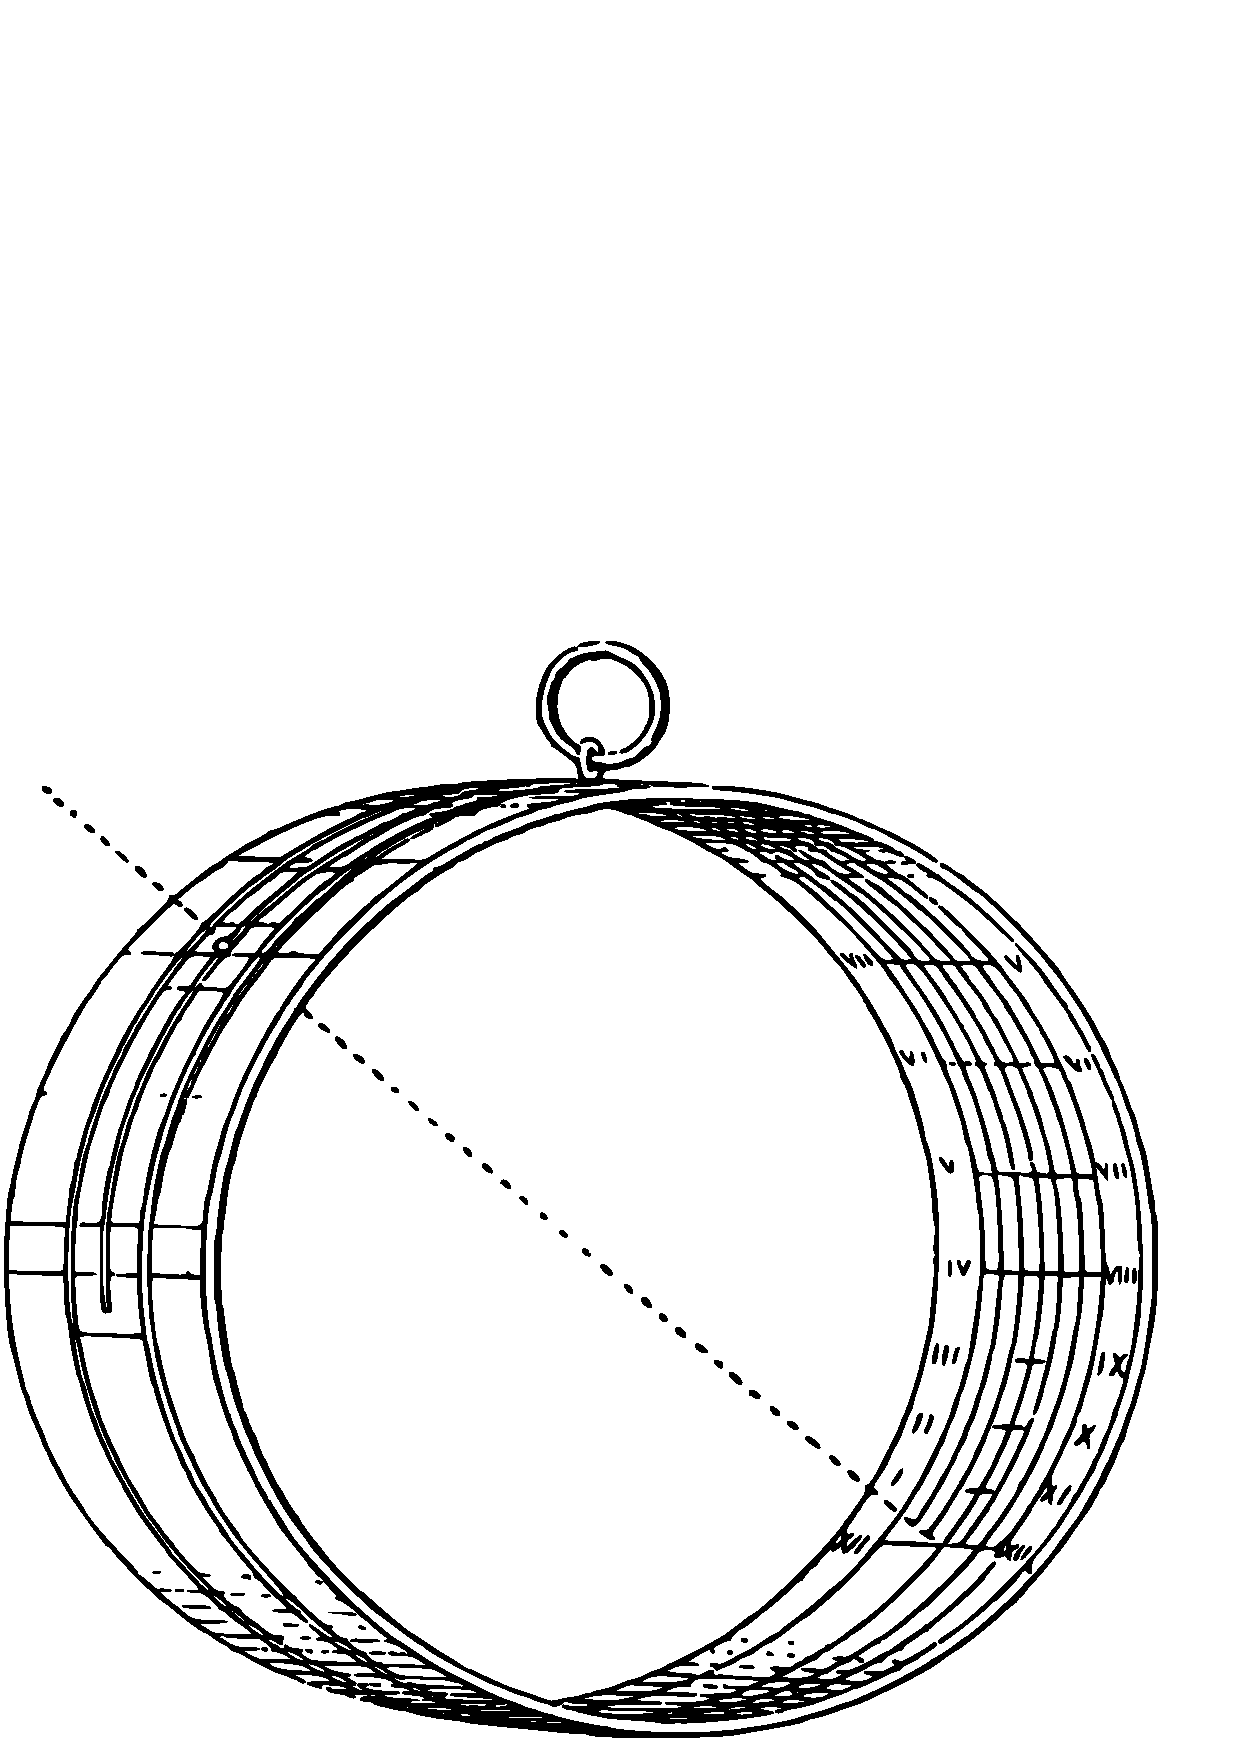
\includegraphics
[height=\ifPaper 8cm\else.7\textheight\fi]{./images/illus367}}
\label{illus:367}
\end{figure*}
The \emph{sun-ring}\index{Sun-rings|(} or \emph{ring-dial}\index
{Ring-Dial|(} is another instrument for measuring
solar time\footnote
{See Ozanam\index{Ozanam@Ozanam's \textit{Récréations}}, 1803 edition,
vol.~\textsc{iii}, p.~317; 1840 edition, p.~526.}.
One of the simplest type is figured in the
% original reads "diagram below" but in print format we hit a
% varioref page-break loop :(
\ifPaper accompanying diagram\else
diagram \vpageref[below]{illus:367}\fi.
The sun-ring consists of a thin brass band,
about a quarter of an inch wide, bent into the shape of a
circle, which slides between two fixed circular rims---the radii
of the circles being about one inch. At one point of the band
there is a hole; and when the ring is suspended from a fixed
\PG----File: 368.png------------------------------------------------------
point attached to the rims so that it hangs in a vertical plane
containing the sun, the light from the sun shines through this
hole and makes a bright speck on the opposite inner or concave
surface of the ring. On this surface the hours are
marked, and, if the ring is properly adjusted, the spot of light
will fall on the hour which indicates the solar time. The
adjustment for the time of year is made as follows. The rims
between which the band can slide are marked on their outer
or convex side with the names of the months, and the band
containing the hole must be moved between the rims until
the hole is opposite to that month for which the ring is being
used.

For determining times near noon the instrument is reliable,
but for other hours in the day it is accurate only if the time
of year is properly chosen, usually near one of the equinoxes.
This defect may be corrected by marking the hours on a
curved brass band affixed to the concave surface of the rims.
I possess two specimens of rings of this kind. These rings
were distributed widely. Of my two specimens, one was
bought in the Austrian Tyrol and the other in London.
Astrolabes and sea-rings can be used as sun-rings\index
{Ring-Dial|)}\index{Sun-rings|)}.

\phantomsection
\addcontentsline{toc}{subsection}{Water-clocks, Sand-clocks,
Graduated Candles}
\emph{Clepsydras}\index{Clepsydras} or water-clocks\index
{Water-clocks}\index{Clocks|(}, and \emph{hour-glasses}\index{Hour-glasses}
or sand-clocks\index{Sand-clocks},
afford other means of measuring time. The time occupied
by a given amount of some liquid or sand in running
through a given orifice under the same conditions is always
the same, and by noting the level of the liquid which has
run through the orifice, or which remains to run through it,
a measure of time can be obtained.

The burning of graduated candles gives another way of
measuring time, and we have accounts of those used by Alfred\index
{Alfred the Great}
the Great for the purpose. Incense sticks were used by the
Chinese in a similar way.

\phantomsection
\addcontentsline{toc}{subsection}{Clocks and Watches}
Modern \emph{clocks} and \emph{watches}\index{Watches}\footnote
{See \textit{Clock and Watch Making} by Lord Grimthorpe\index
{Grimthorpe on Clocks}, 7th edition, London, 1883.}
comprise a train of wheels
\PG----File: 369.png------------------------------------------------------
turned by a weight, spring, or other motive power, and regulated
by a pendulum, balance, fly-wheel, or other moving body
whose motion is periodic and time of vibration constant.
The direction of rotation of the hands of a clock was selected
originally so as to make the hands move in the same direction
as the shadow on a sun-dial whose face is horizontal---the dial
being situated in our hemisphere.

The invention of clocks with wheels is attributed by tradition
to Pacificus\index{Pacificus on Clocks} of Verona, circ.\ 850,
and also to Gerbert\index{Gerbert}, who
is said to have made one at Magdeburg in 996: but there is
reason to believe that these were sun-clocks. The earliest
wheel-clock of which we have historical evidence was one sent
by the Sultan of Egypt in 1232 to the Emperor Frederick~II\index
{Frederick II of Germany},
though there seems to be no doubt that they had been made
in Italy at least fifty years earlier.

The oldest clock in England of which we know anything
was one erected in 1288 in or near Westminster Hall out of a
fine imposed on a corrupt Lord Chief Justice. The bells, and
possibly the clock, were staked by Henry~VIII\index{Henry VIII of England}
on a throw of
dice and lost, but the site was marked by a sun-dial, destroyed
about sixty years ago, and bearing the inscription \emph{Discite justiciam
moniti}. In 1292 a clock was erected in Canterbury
Cathedral at a cost of \pounds30. One erected at Glastonbury Abbey
in 1325 is at present in the Kensington Museum and is in
regular action. Another made in 1326 for St Alban's Abbey
showed the astronomical phenomena, and seems to have been
one of the earliest clocks that did so. One put up at Dover in
1348 is still in good working order. The clocks at Peterborough
and Exeter were of about the same date, and portions of them
remain \emph{in situ}. Most of these early clocks were regulated
by horizontal balances: pendulums being then unknown. Of
the elaborate clocks of a later date, that at Strasburg made
by Dasypodius\index{Dasypodius} in 1571, and that at Lyons constructed by
Lippeus\index{Lippeus} in 1598, are especially famous: the former was
restored in 1842, though in a manner which destroyed most of
the ancient works.

\PG----File: 370.png------------------------------------------------------
In 1370, Vick\index{Vick on Clocks} constructed a clock for
Charles~V\index{Charles V of Germany} with
a weight as motive power and a vibrating escapement---a
great improvement on the rough time-keepers of an
earlier date.

The earliest clock regulated by a pendulum seems to have
been made in 1621 by a clockmaker named Harris\index
{Harris on pendulum clock}, of Covent
Garden, London, but the theory of such clocks is due to
Huygens\index{Huygens}\footnote
{\textit{Horologium Oscillatorium}, Paris, 1673.}.
Galileo\index{Galileo on Pendulum} had discovered previously the isochronism
of a pendulum, but did not apply it to the regulation of the
motion of clocks. Hooke\index{Hooke on Timepieces} made such clocks,
and possibly discovered independently this use of the pendulum: he
invented or re-invented the anchor pallet.

A watch\index{Watches} may be defined as a clock which will go in any
position. Watches, though of a somewhat clumsy design, were
made at Nuremberg by P.~Hele\index{Hele, P.} early in the sixteenth
century---the motive power being a ribbon of steel, wound round a
spindle, and connected at one end with a train of wheels which
it turned as it unwound---and possibly a few similar time-pieces
had been made in the previous century. By the end of
the sixteenth century they were not uncommon. At this time
they were usually made in the form of fanciful ornaments
such as skulls, or as large pendants, but about 1620 the
flattened oval form was introduced, rendering them more
convenient to carry in a pocket or about the person. In the
seventeenth century their construction was greatly improved,
notably by the introduction of the spring balance by Huygens\index{Huygens}
in 1674, and independently by Hooke\index{Hooke on Timepieces} in 1675---both
mathematicians having discovered that small vibrations of a coiled
spring, of which one end is fixed, are practically isochronous.
The fusee had been used by R.~Zech\index{Zech, R.} of Prague in 1525, but
was re-invented by Hooke\index{Hooke on Timepieces}.

Clocks and watches are usually moved and regulated in
the manner indicated above. Other motive powers and other
\PG----File: 371.png------------------------------------------------------
devices for regulating the motion may be met with occasionally.
Of these I may mention a clock in the form of a cylinder,
usually attached to another weight as in Atwood's machine,
which rolls down an inclined plane so slowly that it takes
twelve hours to roll down, and the highest point of the face
always marks the proper hour\footnote
{Ozanam\index{Ozanam@Ozanam's \textit{Récréations}}, 1803 edition,
vol.~\textsc{ii}, p.~39; 1840 edition, p.~212; or \textit{La
Nature}, Jan.~23, 1892, pp.~123, 124.}.

A water-clock\index{Water-clocks} made on a somewhat similar plan is
described by Ozanam\footnote
{Ozanam\index{Ozanam@Ozanam's \textit{Récréations}}, 1803 edition,
vol.~\textsc{ii}, p.~68; 1840 edition, p.~225.} as one of the sights of
Paris at the beginning of
the last century. It was formed of a hollow cylinder divided
into various compartments each containing some mercury, so
arranged that the cylinder descended with uniform velocity
between two vertical pillars on which the hours were marked
at equidistant intervals.

Other ingenious ways of concealing the motive power
have been described in the columns of \textit{La Nature}\footnote
{See especially the volumes issued in 1874, 1877, and 1878.}. Of
such mysterious timepieces the following are not uncommon
examples, and probably are known to most readers of this
book. One kind of clock consists of a glass dial suspended
by two thin wires; the hands however are of metal, and the
works are concealed in them or in the pivot. Another kind
is made of two sheets of glass in a frame containing a spring
which gives to the hinder sheet a very slight oscillatory
motion--imperceptible except on the closest scrutiny--and
each oscillation moves the hands through the requisite angles.
Some so-called perpetual motion timepieces were described
above \vpagerefrange{page:PerpClockStart}{page:PerpClockEnd}.
Lastly, I have seen in France a clock
the hands of which were concealed at the back of the dial, and
carried small magnets; pieces of steel in the shape of insects
were placed on the dial, and, following the magnets, served to
indicate the time\index{Clocks|)}.

\phantomsection
\addcontentsline{toc}{section}{Watches as Compasses}
The position of the sun relative to the points of the compass
\PG----File: 372.png------------------------------------------------------
determines the solar time. Conversely, if we take the time
given by a watch as being the solar time---and it will differ
from it by only a few minutes at the most---and we observe
the position of the sun, we can find the points of the compass\index
{Compasses, Watches as|(}\index
{Watches as Compasses@\nobreak--- as Compasses|(}\footnote
{The rule is given by W.H.~Richards\index{Richards on use of compass},
\textit{Military Topography}, London, 1883, p.~31, though it is not stated
quite correctly. I do not know who first enunciated it.}.
To do this it is sufficient to point the hour-hand to the sun,
and then the direction which bisects the angle between the
hour and the figure \textsc{xii} will point due south. For instance,
if it is four o'clock in the afternoon, it is sufficient to point
the hour-hand (which is then at the figure \textsc{iiii}) to the sun, and
the figure \textsc{ii} on the watch will indicate the direction of south.
Again, if it is eight o'clock in the morning, we must point the
hour-hand (which is then at the figure \textsc{viii}) to the sun, and
the figure \textsc{x} on the watch gives the south point of the
compass.

Between the hours of six in the morning and six in the
evening the angle between the hour and \textsc{xii} which must be
bisected is less than $180^{\circ}$, but at other times the angle to be
bisected is greater than $180^{\circ}$; or perhaps it is simpler to say
that at other times the rule gives the north point and not the
south point.

The reason is as follows. At noon the sun is due south,
and it makes one complete circuit round the points of the
compass in $24$ hours. The hour-hand of a watch also makes
one complete circuit in $12$ hours. Hence, if the watch is held
in the plane of the ecliptic with its face upwards, and the
figure \textsc{xii} on the dial is pointed to the south, both the hour-hand
and the sun will be in that direction at noon. Both
move round in the same direction, but the angular velocity
of the hour-hand is twice as great as that of the sun. Hence
the rule. The greatest error due to the neglect of the equation
of time is less than $2^{\circ}$. Of course in practice most people,
instead of holding the face of the watch in the ecliptic, would
\PG----File: 373.png------------------------------------------------------
hold it horizontal, and in our latitude no serious error would
be thus introduced.

In the southern hemisphere where at noon the sun is due
north the rule requires modification. In such places the hour-hand
of a watch (held face upwards in the plane of the ecliptic)
and the sun move in opposite directions. Hence, if the watch
is held so that the figure \textsc{xii} points to the sun,
then the direction which bisects the angle between the hour of the day
and the figure \textsc{xii} will point due north\index
{Compasses, Watches as|)}\index{Watches as Compasses@\nobreak--- as Compasses|)}.

\PG----File: 374.png------------------------------------------------------



% CHAPTER XIV.
\UseChapterXIVHeadings

\chapter{Matter and Ether Theories.}

\textsc{Matter}, like space and time, cannot be defined, but either\chapindex
{Matter, Constitution of}
the statement that matter is whatever occupies space or the\chapindex
{Atomic@\textsc{Atomic Theories}}
statement that it is anything which can be seen, touched, or
weighed, suggests its more important characteristics to anyone
already familiar with it.

The means of measuring matter and some of its properties
are treated in most text-books on mechanics, and I do not
propose to discuss them. I confine the chapter to an account
of some of the hypotheses by physicists as to the
ultimate constitution of matter, but I exclude metaphysical
conjectures, which from their nature are mere assertions incapable
of proof and are not subject to mathematical analysis.
The question is intimately associated with the explanation of
the phenomena of attraction, light, chemistry, electricity, and
other branches of physics.

I commence with a list of some of the more plausible of
the hypotheses formerly proposed which accounted for the
obvious properties of matter, and shall then discuss how far
they explain or are consistent with other facts\footnote
{I have based my account mainly on \textit{Recent Advances in Physical
Science}, by P.G.~Tait\index{Tait}, Edinburgh, 1876 (chaps,~\textsc{xii},
\textsc{xiii}); and on the article \textit{Atom} by J.~Clerk Maxwell\index
{Maxwell, J. Clerk} in the Encyclopaedia Britannica or
his \textit{Collected Works}, vol.~\textsc{ii}, pp.~445--484: see also
W.M.~Hicks's\index{Hicks on Matter}
address, Report of the British Association (Ipswich meeting), 1895,
vol.~\textsc{lxv}, pp.~595--606. For the more recent speculations see
J.J.~Thomson\index{Thomson, J.J.}, \textit{Electricity and Matter},
Westminster, 1904, and J.~Larmor\index{Larmor on Electrons}, \textit{Aether
and Matter}, Cambridge, 1900.}. The interest
\PG----File: 375.png------------------------------------------------------
of the list is largely historical, for within the last few years
new views as to the constitution of matter have been propounded,
but the details of these more recent hypotheses are
so complicated and technical that only professional mathematicians
can understand them. Accordingly I allude to them
only briefly.

\section[Hypothesis of Continuous Matter][Matter and Ether Theories]%
{Hypothesis of Continuous Matter}
It may be\index{Continuity of Matter}%
\index{Matter, Hyp@\nobreak--- Hypotheses on|(}
supposed that matter is homogeneous and continuous, in
which case there is no limit to the infinite divisibility of
bodies. This view was held by Descartes\index{Descartes}\footnote
{Descartes, \textit{Principia}, vol.~\textsc{ii}, pp.~18, 23.}.

This conjecture is consistent with the facts deducible by
untrained observation, but there are many other phenomena
for which it does not account; moreover there seems to be no
way of reconciling such a structure of matter either with the
facts of chemical changes or with the results of spectrum
analysis\index{Spectrum Analysis}. At any rate the theory must be regarded
as extremely improbable.

\section[Atomic Theories][Matter and Ether Theories]{Atomic Theories}
If matter is not continuous we
must suppose that every body is composed of aggregates of
molecules. If so, it seems probable that each such molecule is
built up by the association of two or more atoms, that the
number of kinds of atoms is finite, and that the atoms of any
particular kind are alike. As to the nature of the atoms the
following hypotheses have been made.

\subsection[Popular Atomic Hypothesis][Matter and Ether Theories]%
{Popular Atomic Hypothesis} The popular view is that
every atom of any particular kind is a minute indivisible
article possessing definite qualities, everlasting in its form and
properties, and infinitely hard.

This statement is plausible, but the difficulties to which it
leads appear to be insuperable. In fact we have reason to
think that the atoms which form a molecule are composite
systems in incessant vibration at a rate characteristic of the
molecule, and it is most probable that they are elastic.

\PG----File: 376.png------------------------------------------------------
Newton\index{Newton} seems to have hazarded a conjecture of this kind
when he suggested\footnote
{Newton, \textit{Principia}, bk.~\textsc{ii}, prop.~50.}
that the difficulties, connected with the
fact that the velocity of sound\index{SoundVel@\nobreak--- Velocity of} was
one-ninth greater than that
required by theory, might be overcome if the particles of air
were little rigid spheres whose distance from one another under
normal conditions was nine times the diameter of any one of
them. This was ingenious, but obviously the view is untenable,
because, if such a structure of air existed, the air could not
be compressed beyond a certain limit, namely, about $1/1021$st
part of its original volume, which has been often exceeded.
The true explanation of the difficulty noticed by Newton was
given by Laplace\index{Laplace on velocity of sound}.

\subsection[Boscovich's Hypothesis][Matter and Ether Theories]%
{Boscovich's Hypothesis}
In 1759 Boscovich suggested\index{Boscovich on Matter}\footnote
{\textit{Philosophiae naturalis Theoria redacta ad unicam Legem Virium},
Vienna, 1759.}
that the facts might be explained by supposing that an atom
was an infinitely small indivisible mass which was a centre of
force---the law of force being attractive for sensible distances,
alternately attractive and repulsive for minute distances, and
repulsive for infinitely small distances. In this theory all
action between bodies is action at a distance.

He explained the apparent extension of bodies by saying
that two parts are consecutive (or similarly that two bodies are
in contact) when the nearest pair of atoms in them are so close
to one another that the repulsion at any point between them
is sufficiently great to prevent any other atom coming between
them. It is essential to the theory that the atom shall have
a mass but shall not have dimensions.

This hypothesis is not inconsistent with any known facts,
but it has been described, perhaps not unjustly, as a mere
mathematical fiction, and certainly it is opposed to the apparent
indications of our senses. At any rate it is artificial, though
it may be a prejudice to regard that as an argument against
its adoption. To some extent this view was accepted by
Faraday\index{Faraday on Matter}.

\PG----File: 377.png------------------------------------------------------
Lord Kelvin\index{Kelvin}, better known as Sir William Thomson, has
shown\footnote
{\textit{Proceedings of the Royal Society of Edinburgh}, April~21, 1862,
vol.~\textsc{iv}, pp.~604--606.}
that, if we assume the existence of gravitation, then
each of the above hypotheses will account for cohesion.

\subsection[Hypothesis of an Elastic Solid Ether. Labile Ether]%
[Matter and Ether Theories]{Hypothesis of an Elastic Solid Ether}
Some physicists\index{Ether Theories|(}
have tried to explain the known phenomena by properties of
the medium through which our impressions are derived. By
postulating that all space is filled with a medium possessed of
many of the characteristics of an elastic solid, it has been
shown by Fresnel\index{Fresnel on Ether}, Green\index{Green on Ether},
Cauchy\index{Cauchy}, Neumann\index{Neumann on Ether},
MacCullagh\index{MacCullagh on Ether}, and
others that a large number of the properties of light and
electricity may be explained. In spite of the difficulties to
which this hypothesis necessarily leads, and of its inherent
improbability, it has been discussed by Stokes\index{Stokes on Ether},
Lamé\index{Lame@Lamé}, Boussinesq\index{Boussinesq on Ether},
Sarrau\index{Sarrau on Ether}, Lorenz\index{Lorentz on Ether},
Lord Rayleigh\index{Rayleigh}, and Kirchhoff\index{Kirchhoff on Ether}.

This hypothesis has been modified and rendered somewhat
more plausible by von~Helmholtz\index{Helmholz}\index{Von Helmholz},
Lommel\index{Lommel on Ether}, Ketteler\index{Ketteler on Ether}\footnote
{\textit{Theoretische Optik}, Braunschweig, 1885.}, and
Voigt\index{Voigt on Ether}, who based their researches on the assumption of
a mutual reaction between the ether and the material molecules
located in it: on this view the problems connected with refraction
and dispersion have been simplified. Finally, Sir
William Thomson\index{Kelvin}, in his Baltimore Lectures, 1885, suggested
a mechanical analogue to represent the relations between
matter and this ether, by which a possible constitution of the
ether can be realized. He also suggested later a form of
\emph{labile ether}\index{Labile Ether}, from whose properties most of the
more familiar physical phenomena can be deduced, provided the arrangement
can be considered stable; a labile ether is an elastic solid,
and its properties in two dimensions may be compared with
those of a soap-bubble film, in three dimensions.

It is, however, difficult to criticise any of these hypotheses
as a theory of the constitution of matter until the arrangement
of the atoms or their nature is more definitely expressed.

\PG----File: 378.png------------------------------------------------------


\section[Dynamical Theories][Matter and Ether Theories]{Dynamical Theories}
In recent years the suggestion
has been made that the so-called atoms may be forms of
motion (\Eg~permanent eddies) in one elementary material
known as the ether; on this view all the atoms are constituted
of the same matter, but the physical conditions are
different for the different kinds of atoms. It has been said
that there is an initial difficulty in any such hypothesis, since
the all-pervading elementary fluid must possess inertia, so that
to explain matter we assume the existence of a fluid possessing
one of the chief characteristics of matter. This is true as far
as it goes, but it is not more unreasonable than to attribute
all the fundamental properties of matter to the atoms themselves,
as is done by many writers. The next paragraph
contains a statement of one of the earliest attempts to
formulate a dynamical atomic hypothesis.

\subsection[The Vortex Ring Hypothesis][Matter and Ether Theories]%
{The Vortex Ring Hypothesis} This hypothesis assumes
that each atom is a vortex ring in an incompressible frictionless
homogeneous fluid.

Vortex rings\index{Vortex rings}---though, since friction is brought into
play, of an imperfect character---can be produced in air by many
smokers. Better specimens can be formed by taking a
cardboard box in one side of which a circular hole is cut,
filling it with smoke, and hitting the opposite side sharply.
The tendency of the particles forming a ring to maintain their
annular connection may be illustrated by placing such a box
on one side of a room in a direct line with the flame of a
lighted candle on the other side. If properly aimed, the ring
will travel across the room and put out the flame. If the box
is filled only with air, so that the ring is not visible, the
experiment is more effective.

In 1858 von Helmholtz\index{Helmholtz}\index{Von Helmholz}\footnote
{\textit{Crelle's Journal}, 1858, vol.~\textsc{lv}, pp.~25--55; translated
by Tait\index{Tait} in the \textit{Philosophical Magazine}, June, 1867,
supplement, series~4, vol.~\textsc{xxxiii}, pp.~485--512.}
showed that a closed vortex filament
in a perfect fluid is indestructible and retains certain
\PG----File: 379.png------------------------------------------------------
characteristics always unaltered. In 1867 Sir William Thomson\index{Kelvin}
propounded\footnote
{\textit{Proceedings of the Royal Society of Edinburgh}, Feb.~18, 1867,
vol.~\textsc{vi}, pp.~94--105.} the idea that matter consists of vortex
rings in a fluid which fills space. If the fluid is perfect we could
neither create new vortex rings nor destroy those already
created, and thus the permanence of the atoms is explained.
Moreover the atoms would be flexible, compressible, and in
incessant vibration at a definite fundamental rate. This rate
is very rapid, and Sir William Thomson gave the number of
vibrations per second of a sodium ring as probably being
greater than $10^{14}$.

By a development of this hypothesis Prof.\ J.J.~Thomson\index
{Thomson, J.J.}\footnote
{\textit{A Treatise on the Motion of Vortex Rings}\index{Vortex rings},
Cambridge, 1883.} showed, some years ago, that chemical combination may be
explained. He supposed that a molecule of a compound is
formed by the linking together of vortex filaments representing
atoms of different elements: this arrangement may be
compared with that of helices on an anchor ring. For stability
not more than six filaments may be combined together, and
their strengths must be equal. Another way of explaining
chemical combination on the vortex atom hypothesis has been
suggested by W.M.~Hicks\index{Hicks on Matter}. It is known\footnote
{See a memoir by M.J.M.~Hill\index{Hill, M.J.M.} in the \textit{Philosophical
Transactions of the Royal Society}, London, 1894, part~i, pp.~213--246.}
that a spherical
mass of fluid, whose interior possesses vortex motion, can
move through liquid like a rigid sphere, and he has shown
that one of these spherical vortices\index{Vortex spheres@\nobreak--- Spheres}
can swallow up another, thus forming a compound element.

\subsection[The Vortex Sponge Hypothesis][Matter and Ether Theories]%
{The Vortex Sponge Hypothesis}
Any vortex\index{Vortex sponges@\nobreak--- Sponges} atom
hypothesis labours under the difficulty of requiring that
the density of the fluid ether shall be comparable with
that of ordinary matter. In order to obviate this and
at the same time to enable it to transmit transversal
radiations Sir William Thomson suggested what has been
\PG----File: 380.png------------------------------------------------------
termed, not perhaps very happily, the vortex sponge hypothesis\index
{Vortex sponges@\nobreak--- Sponges}\footnote
{\textit{Philosophical Magazine}, London, October, 1887, series 5,
vol.~\textsc{xxiv}, pp.~342--353.}:
this rests on the assumption that laminar motion
can be propagated through a turbulently moving inviscid
liquid. The mathematical difficulties connected with such
motion have prevented an adequate discussion of this hypothesis,
and I therefore confine myself to merely mentioning it.

These hypotheses, of vortex motion in a fluid, account for
the indestructibility of matter and for many of its properties.
But in order to explain statical electrical attraction it would
seem necessary to suppose that the ether is elastic; in other
words, that an electric field must be a field of strain. If so,
complete fluidity in the ether would be impossible, and hence
the above theories are now regarded as untenable.

\subsection[The Ether-Squirts Hypothesis][Matter and Ether Theories]%
{The Ether-Squirts Hypothesis}
Prof.\ Karl Pearson\index{Pearson on Ether-Squirts}\index
{Ether-Squirts}\footnote
% switched with footnote on next page as per errata sheet
{\textit{American Journal of Mathematics}, 1891, vol. \textsc{xiii},
pp.~309--362.}
has suggested another dynamical theory in which an atom is
conceived as a point at which ether is pouring into our space
from space of four dimensions.

If an observer lived in two dimensional space filled with
ether and confined by two parallel and adjacent surfaces, and
if through a hole in one of these surfaces fresh ether were
squirted into this space, the variations of pressure thereby
produced might give the impression of a hard impenetrable
body. Similarly an ether-squirt from space of four dimensions
into our space might give us the impression of matter.

It seems necessary on this hypothesis to suppose that there
are also ether-sinks, or atoms of negative mass; but as ether-squirts
and ether-sinks would repel one another we may suppose
that the latter have moved out of the universe known to
our senses.

By defining the mass of an atom as the mean rate at which
\PG----File: 381.png---------------------------------------------------
ether is squirting into our space at that point, we can deduce
the Newtonian law of gravitation, and by assuming certain
periodic variations in the rate of squirting we can deduce
some of the phenomena of cohesion, of chemical action, and of
electromagnetism and light. But of course the hypothesis rests
on the assumption of the existence of a world beyond our senses\index
{Ether Theories|)}.

\subsection[The Electron Hypothesis][Matter and Ether Theories]%
{The Electron Hypothesis} MacCullagh, in 1837 and\index{Electrons|(}
1839, proposed to account for optical phenomena on the
assumption of an elastic ether possessing elasticity of the type
required to enable it to resist rotation. This suggestion has
been recently modified and extended by Dr~J.~Larmor\index
{Larmor on Electrons}\footnote
% switched with 2nd footnote on previous page as per errata sheet
{\textit{Philosophical Transactions of the Royal Society}, London, 1894,
pp.~719--822; 1895, pp.~695--743.}, and,
as now enunciated, it accounts for many of the electrical and
magnetic (as well as the optical) properties of matter.

The hypothesis is however very artificial. The assumed
ether is a rotationally elastic incompressible fluid. In this
fluid Larmor\index{Larmor on Electrons} introduces monad electric
elements or \emph{electrons},
which are nuclei of radial rotational strain. He supposes
that these electrons constitute the basis of matter. He
further supposes that an electrical current consists of a procession
of these electrons, and that a magnetic particle is
one in which these entities are revolving in minute orbits.
Dynamical considerations applied to such a system lead to
an explanation of nearly all the more obvious phenomena.
By further postulating that the orbital motion of electrons in
the atom constitute it a fluid vortex it is possible to apply the
hydrodynamical pulsatory theory of Bjerknes\index{Bjerknes}
or Hicks\index{Hicks on Matter} and
obtain an explanation of gravitation.

Thus on this view mass is explained as an electrical manifestation.
Electricity in its turn is explained by the existence
of electrons, that is, of nuclei of strain in the ether, which
are supposed to be in incessant and rapid motion. Whilst, to
render this possible, properties are attributed to the ether
which are apparently inconsistent with our experience of the
space it fills. Put thus, the hypothesis seems very artificial.
\PG----File: 382.png---------------------------------------------------
Perhaps the utmost we can say for it is that, from some points
of view, it may, so far as analysis goes, be an approximation
to the true theory; in any case much work will have to be
done before it can be considered established even as a working
hypothesis.

\phantomsection
\addcontentsline{toc}{subsection}{Speculations due to
investigations on Radio-activity}
Most of the above was written in 1891. Since then
investigations on radio-activity have opened up new avenues
of conjecture which tend to strengthen the electron theory as
a working hypothesis. More than thirty years ago Clerk
Maxwell\index{Maxwell, J. Clerk} had shown that light and electricity
were closely
connected phenomena. It was then believed that both were
due to waves in the hypothetical ether, but it was supposed
that the phenomena of matter on the one side and of light
and electricity on the other were sharply distinguished one
from the other. The differences, however, between matter and
light tend to disappear as investigations proceed. In 1895
Röntgen established the existence of rays which could produce
light, which had the same velocity as light, which were not
affected by a magnet, and which could traverse wood and certain
other opaque substances like glass. A year later Becquerel\index
{Becquerel Rays}
showed that uranium was constantly emitting rays which,
though not affecting the eye as light, were capable of producing
an image on a photographic plate. Like Röntgen
rays\index{Rontgen@Röntgen Rays} they can go through thin sheets of metal;
like heat rays
they burn the skin; like electricity they generate ozone from
oxygen. Passed into the air they enable it to conduct the
electric current. Their speed has been measured and found
to be rather more than half that of light and electricity.
It was soon found that thorium possessed a similar property,
but in 1903 Prof.\ Curie\index{Curie on radio-activity} showed that
radium possessed radio-activity
to an extent previously unsuspected in any body, and
in fact the rays were so powerful as to make the substance
directly visible. Further experiments showed that numerous
bodies are radio-active, but the effects are so much more
marked in radium that it is convenient to use that substance
for most experimental purposes.

\PG----File: 383.png---------------------------------------------------
Radium gives off no less than three kinds of rays besides
a radio-active emanation. In these discharges there appears
to be a gradual change from what had been supposed to be
an elementary form of matter to another. This leads to the
belief that of the known forms of matter some, perhaps even
all, are not absolutely stable. On the other hand, it may be
that only radio-active bodies are unstable, and that in their
disintegration we are watching the final stage in the evolution
of stable and constant forms of matter. It may, however, in
any case turn out that some, or perhaps all, of the so-called
elements may be capable of resolution into different combinations
of electrons or electricity.

At an earlier date J.J.~Thomson\index{Thomson, J.J.} had concluded that the
glow, seen when an electric current passes through a high
vacuum tube, is due to a rush of minute particles across the
tube. He calculated their weight, their velocity, and the
charge of electricity transported by or represented by them,
and found these to be constant. They were deflected like
Becquerel rays\index{Becquerel Rays}. All space seems to contain them,
and electricity,
if not identical with them, is at least carried by them.
This suggested that these minute particles might be electrons.
If so, they might thus give the ultimate explanation of electricity
as well as matter, and the atom of the chemist would
be not an irreducible unit of matter, but a system comprising
numerous such minute particles. These conclusions are consistent
with those subsequently deduced from experiments
with radium. In 1904 the hypothesis was carried one stage
further. In that year J.J.~Thomson\index{Thomson, J.J.} investigated
the conditions
of stability of certain systems of revolving particles;
and on the hypothesis that an atom of matter consists of a
number of particles carrying negative charges of electricity
revolving in orbits within a sphere of positive electrification\index
{Electrons|)}
he deduced many of the properties of the different chemical
atoms corresponding to different possible stable systems of
this kind. His scheme led to results agreeing closely with
the results of Mendeléeff's\index{Mendel@Mendeléeff} periodic hypothesis.
An interesting
\PG----File: 384.png------------------------------------------------------
consequence of this view is that Franklin's\index{Franklin, B.} description
of electricity as subtle particles pervading all bodies, may turn
out to be substantially correct. It is also remarkable that
corpuscles somewhat analogous to those whose existence was
suggested in Newton's\index{Newton} corpuscular theory of light should be
now supposed to exist in cathode and Becquerel rays\index{Becquerel Rays}.

\subsection[The Bubble Hypothesis][Matter and Ether Theories]%
{The Bubble Hypothesis\footnote
{O.~Reynolds\index{Reynolds, O.}, \textit{Submechanics of the Universe},
Cambridge, 1903.}}
The difficulty of conceiving\index{Bubble Theory of Matter}
the motion of matter through a solid elastic medium has been
met in another way, namely, by suggesting that what we call
matter is a deficiency of the ether, and that this region of
deficiency can move through the ether in a manner somewhat
analogous to that in which a bubble can move in a liquid.
To express this in technical language we may suppose the
ether to consist of an arrangement of minute uniform spherical
grains piled together so closely that they cannot change their
neighbours, although they can move relatively one to another.
Places where the number of grains is less or greater than the
number necessary to render the piling normal, move through
the medium, as a wave moves through water, though the
grains do not move with them. Places where the ether is in
excess of the normal amount would repel one another and
move away out of our ken, but places where it is below the
normal amount would attract each other according to the law
of gravity, and constitute particles of matter which would
be indestructible. It is alleged that the theory accounts for
the known phenomena of gravity, electricity, and light, provided
the size of its grains is properly chosen. Reynolds\index{Reynolds, O.}
has calculated that for this purpose their diameter should be
rather more than $5 \times 10^{-18}$ centimetres, and that the pressure
in the medium would be about $10^4$ tons per square centimetre.
This theory is in itself more plausible than the electron
hypothesis, but its consequences have not yet been fully
worked out\index{Matter, Hyp@\nobreak--- Hypotheses on|)}.
\PG----File: 385.png---------------------------------------------------

\ThoughtBreakSpace
\phantomsection
\addcontentsline{toc}{section}{Conjectures as to the cause of Gravity}
\markright{The cause of Gravity}
Returning from these novel hypotheses to the classical
theories of matter, we may now proceed a step further.
Before a hypothesis on the structure of matter can be ranked
as a scientific theory we may reasonably expect it to afford
some explanation of three facts. These are (\emph{a})~the Newtonian
law of attraction; (\emph{b})~the fact that there are only a finite
number of ultimate kinds of matter---such as oxygen, iron, etc.---which
can be arranged in a series such that the properties of
the successive members are connected by a regular law; and
(\emph{c})~the main results of spectrum analysis.

In regard to the first point (\emph{a}), we can say only that none\index
{Attraction, Law of|(}\index{Gravity@\textsc{Gravity}, Hypotheses on|(}
of the above theories are inconsistent with the known laws of
attraction; and as far as the ether-squirts, the electron, and
the bubble hypotheses are concerned, they have been elaborated
into a form from which the gravitational law of attraction
can be deduced. But we may still say that as to the cause
of gravity---or indeed of force---we know nothing.

Newton\index{Newton}, in his Letters to Bentley\index{Bentley, Newton to},
while declaring his
ignorance of the cause of gravity, refused to admit the possibility
of force acting at a finite distance through a vacuum.
``You sometimes speak of gravity,'' said he\footnote
{Letter dated Jan.~17, 1693. I quote from the original, which is in
the Library of Trinity College, Cambridge; it is printed in the \textit
{Letters to Bentley}, London, 1756, p.~20.\label{ibid:17}}, ``as essential
and inherent to matter: pray do not ascribe that notion to
me, for the cause of gravity is what I do not pretend to
know.'' And in another place he wrote\footnote
{Letter dated Feb.~25, 1693; \ibidref{ibid:17}{\textit
Letters to Bentley}, pp.~25, 26. }, ``'Tis inconceivable,
that inanimate brute matter should (without the mediation of
something else which is not material) operate upon and affect
other matter without mutual contact; as it must if gravitation
in the sense of Epicurus\index{Epicurus on Gravitation}, be essential
and inherent in it\textellipsis\ That gravity should be innate,
inherent, and essential to
matter, so that one body may act upon another at a distance
thro' a vacuum, without the mediation of anything else, by
and through which their action and force may be conveyed
\PG----File: 386.png---------------------------------------------------
from one to another, is to me so great an absurdity, that I
believe no man who has in philosophical matters a competent
faculty of thinking can ever fall into it. Gravity must be
caused by an agent acting constantly according to certain
laws, but whether this agent be material or immaterial, I have
left to the consideration of my readers.''

I have already alluded to conjectural explanations of
gravity dependent on the ether-squirts, the electron, and the
bubble hypotheses. Of other conjectures as to the cause of
gravity, three, which do not involve the idea of force acting
at a distance, may be here mentioned:

(1)\quad The first of these conjectures was propounded by
Newton\index{Newton} in the \emph{Queries} at the end of his \textit
{Opticks}, where he
suggested as a possible explanation the existence of a stress
in the ether surrounding a particle of matter\footnote
{Quoted by S.P.~Rigaud\index{Rigaud, S.P.} in his \textit{Essay} on the
\textit{Principia}, Oxford,
1838, appendix, pp.~68--70. On other guesses by Newton see Rigaud,
text, pp.~61--62, and references there given.}.

This has been elaborated on a statical basis by Maxwell\index
{Maxwell, J. Clerk}, who showed\footnote
{Article \emph{Attraction}, in \textit{Encyclopaedia Britannica},
or \textit{Collected Works}, vol.~\textsc{ii}, p.~489. }
that the stress would have to be at least 3000
times greater than that which the strongest steel would
support. Sir William Thomson (Lord Kelvin\index{Kelvin}) has
suggested\footnote
{\textit{Proceedings of the Royal Society of Edinburgh}, Feb.~7, 1870,
vol.~\textsc{vii}, pp.~60--63.}
a dynamical way of producing the stress by supposing that
space is filled with an incompressible fluid, constantly being
annihilated by each atom of matter at a rate proportional to
its mass, a constant supply being kept up at an infinite
distance. It is true that this avoids Maxwell's difficulty, but
we have no right to introduce such sinks and sources of fluid
unless we have other grounds for believing in their existence.
The conclusion is that Newton's conjecture is very improbable
unless we adopt the ether-squirts theory: on that hypothesis
it is a plausible explanation.

\PG----File: 387.png------------------------------------------------------
I should add that Maclaurin\index{Maclaurin on Newton} implies\footnote
{\textit{An Account of Sir Isaac Newton's Philosophical Discoveries}, London,
1748, p.~111.} that though the
above explanation was Newton's\index{Newton} early opinion, yet his final
view was that he could not devise any tenable hypothesis
about the cause of gravitation.

(2)\quad In 1782 Le~Sage\index{LeSage@Le Sage on Gravity} of Geneva
suggested\footnote
{\textit{Mémoires de l'Académie des Sciences} for 1782, Berlin, 1784,
pp.~404--432: see also the first two books of his \textit
{Traité de Physique}, Geneva, 1818.} that gravity
was caused by the bombardment of streams of ultramundane
corpuscles. These corpuscles are supposed to come in all
directions from space and to be so small that inter-collisions
are rare.

A body by itself in space would receive on an average as
many blows on one side as on another, and therefore would
have no tendency to move. But, if there are two bodies, each
will screen the other from some of the bombarding corpuscles.
Thus each body will receive more blows on the side remote from
the other body than on the side turned towards it. Hence
the two bodies will be impelled each towards the other.

In order to make this force between two particles vary
directly as the product of their masses and inversely as the
square of the distance between them, Le~Sage\index
{LeSage@Le Sage on Gravity} showed that
it was sufficient to suppose that the mass of a body was proportional
to the area of a section at right angles to the
direction in which it was attracted. This requires that the
constitution of a body shall be molecular, and that the
distances between consecutive molecules shall be very large
compared with the sizes of the molecules. On the vortex
hypothesis we may suppose that the ultramundane corpuscles
are vortex rings.

This is ingenious, and it is possible that if the corpuscles
were perfectly elastic the theory might be tenable\footnote
{See a paper by Sir William Thomson (Lord Kelvin\index{Kelvin}) in the
\textit{Proceedings of the Royal Society of Edinburgh}, Dec.~18, 1871,
vol.~\textsc{vii}, pp.~577--589.}. But
\PG----File: 388.png------------------------------------------------
the results of Maxwell's\index{Maxwell, J. Clerk} numerical calculation show,
first, that the particles must be imperfectly elastic; second, that
merely to produce the effect of the attraction of the earth
on a mass of one pound would require that Le~Sage's\index
{LeSage@Le Sage on Gravity} corpuscles
should expend energy at the rate of at least billions\footnote
{I use billion with the English (and not the French) meaning, that
is, a billion $=10^{12}$.}
of foot-pounds per second; and third, that it is probable that
the effect of such a bombardment would be to raise the
temperature of all bodies beyond a point consistent with our
experience. Finally, it seems probable that the distance
between consecutive molecules would have to be considerably
greater than is compatible with the results given below.

Tait\index{Tait} summed up the objections to these two hypotheses
by saying\footnote
{\textit{Properties of Matter}, London, 1885, art.~164.},
``One common defect of these attempts is\textellipsis that % NB tight ellipsis matches original
they all demand some prime mover, working beyond the
limits of the visible universe or inside each atom: creating or
annihilating matter, giving additional speed to spent corpuscles,
or in some other way supplying the exhaustion
suffered in the production of gravitation. Another defect is
that they all make gravitation a mere difference-effect, as it
were; thereby implying the presence of stores of energy absolutely
gigantic in comparison with anything hitherto observed,
or even suspected to exist, in the universe; and therefore
demanding the most delicate adjustments, not merely to maintain
the conservation of energy which we observe, but to
prevent the whole solar and stellar systems from being instantaneously
scattered in fragments through space. In fact,
the cause of gravitation remains undiscovered.''

(3)\quad There is another conjecture on the cause of gravity
which I may mention\footnote
{See an article by myself in the \textit{Messenger of Mathematics},
Cambridge, 1891, vol.~\textsc{xxi}, pp.~20--24.}.
It is possible that the attraction of
one particle on another might be explained if both of them
rested on a homogeneous elastic body capable of transmitting
\PG----File: 389.png------------------------------------------------
energy. This is the case if our three-dimensional universe rests
in the direction of a fourth dimension on a four-dimensional
homogeneous elastic body (which we may call the ether) whose
thickness in the fourth dimension is small and constant.

The results of spectrum analysis lead us to suppose that
every molecule of matter in our universe is in constant vibration.
On the above hypothesis these vibrations would cause a
disturbance in the supporting space, \IE\ in the ether. This
disturbance would spread out uniformly in all directions; the
intensity diminishing as the square of the distance from the
centre of vibration, but the rate of vibration remaining unaltered.
The transmission of light and radiant heat may be
explained by such vibrations transversal to the direction of
propagation. It is possible that gravity may be caused by
vibrations in the supporting space which are wholly longitudinal
or are compounded of vibrations which are partly longitudinal
and partly transversal in any of the three directions at
right angles to the direction of propagation. If we define the
mass of a molecule as proportional to the intensity of these
vibrations caused by it, then at any other point in space the
intensity of the vibration there would vary as the mass of the
molecule and inversely as the square of the distance from the
molecule; hence, if we may assume that such vibrations of the
medium spreading out from any centre would draw to that
centre a particle of unit mass at any other point with a force
proportional to the intensity of the vibration there, then the
Newtonian law of attraction would follow. This conjecture
is consistent either with Boscovich's hypothesis\index{Boscovich on Matter}
or with the vortex theory. It would be interesting if the results of a
branch of pure mathematics so abstract as the theory of hyperspace
should be found to be closely connected with one of the
most fundamental problems of material science%
\index{Attraction, Law of|)}%
\index{Gravity@\textsc{Gravity}, Hypotheses on|)}.

I should sum up the effect of this discussion on gravity
on the relative probabilities of the hypotheses as to the constitution
of matter enumerated above, by saying that it does
not enable us to discriminate between them.
\PG----File: 390.png------------------------------------------------

\ThoughtBreakSpace
\phantomsection
\addcontentsline{toc}{section}{Conjectures to explain the finite number
of species of Atoms}\markright{Finite number of kinds of Matter}
The fact that the number of kinds of matter\index
{Matter, Kind@\nobreak--- Kinds of, limited|(} (chemical
elements) is finite and the consequences of spectrum analysis
are closely related and may be treated together. The results of
spectrum analysis show that every molecule of any species of
matter, such as hydrogen, vibrates with (so far as we can tell)
exactly equal sets of periods of vibration. This then is one
of the characteristics of the particular kind of matter, and it
is probable that any explanation of why the molecules of each
kind have a definite set of periods of vibration will account
also for the fact that the number of kinds of matter is finite.

Various attempts to explain why the molecules of matter
are capable only of certain definite periods of vibration have
been made, and it may be interesting if I give them
briefly.

(1)\quad To begin with, I may note the conjecture that it
depends on properties of time. This, however, is impossible, for
the continuity of certain spectra proves that in these cases there
is nothing which prevents the period of vibration from taking
any one of millions of different values: thus no explanation
dependent on the nature of time is permissible.

(2)\quad It has been suggested that there may have been a
sorting agency, and only selected specimens of the infinite
number of species formed originally have got into our universe.
The objection to this is that no explanation is offered as to
what has become of the excluded molecules.

(3)\quad The finite number\label{page:373} of species might be explained by
supposing a physical connection to exist between all the molecules
in the universe, just as two clocks whose rates are nearly
the same tend to go at the same rate if their cases are connected.

Maxwell's\index{Maxwell, J. Clerk} objection to this is that we have no
other reason for supposing that such a connection exists, but if we are
living in a space of four dimensions as suggested above in
\hyperlink{chapter.12}{chapter~\textsc{xii}}, this connection does exist,
for all the molecules rest on one and the same body. This body is capable of
transmitting vibrations, hence, no matter how the molecules were
set vibrating originally, they would fall into certain groups,
\PG----File: 391.png------------------------------------------------
and all the members of each group would vibrate at the same
rate. It was the possibility of obtaining thus a physical
connection between the various particles in our universe that
first suggested to me the idea of a supporting medium in a
fourth dimension.

(4)\quad If we accept Boscovich's hypothesis\index{Boscovich on Matter} or
that of an elastic solid ether, and if we may lay it down as axiomatic
that the mass of every sub-atom is the same, we may conceive
that the number of ways of combining the sub-atoms into a
permanent system is limited, and that the period of vibration
depends on the form in which the sub-atoms are combined
into an atom. This view is not inconsistent with any known
facts. I may add that it is probable that the chemical atom
is the essential vibrating system, for the sodium spectrum, to
take one instance, is the same as that of all its compounds.

(5)\quad In the same way we may suppose that the vortex
rings are formed so that they can have only a definite number
of stable forms produced by interlinking or kinking.

(6)\quad Similarly we may modify the popular hypothesis by
treating the atoms as indivisible aggregates of sub-atoms which
are in all respects equal and similar, and can be combined in
only a limited number of forms which are permanent. But
most of the old difficulties connected with the atoms arise
again in connection with the sub-atoms.

(7)\quad I am not aware that Maxwell\index{Maxwell, J. Clerk} discussed any
other hypotheses in connection with this point, but it has been
suggested recently that, if the various forms of matter were
evolved originally out of some one primitive material, then
there may have been periodic disturbances in this matter when
the atoms were being formed, such that they were produced
only at some definite phase in the period\footnote
{See Crookes\index{Crookes@Crookes on Mendeléeff's Laws} on
Mendeléeff's\index{Mendel@Mendeléeff} periodic law, \textit{Nature},
Sept.~2, 1886, vol.~\textsc{xxxiv}, pp.~423--432.}.

Thus, if the disturbance is represented by the swinging of
a pendulum in a resisting medium, it might be supposed that
\PG----File: 392.png------------------------------------------------
the atoms were formed at the points of maximum amplitude,
and we should expect that the atoms successively thrown off
would form a series having the properties of its successive
members connected by a regular periodic law. This conjecture,
when worked out in some detail, led to the conclusion
that some elements which ought to have appeared in the series
were missing, but it was possible to predict their properties
and to suggest the substances with which they were most
likely to be found in combination. Guided by these theoretical
conclusions a careful chemical analysis revealed the fact that
such elements did exist.

That this hypothesis has led to new discoveries is something
in its favour, but I do not wish to be understood to say
that it is a theory which leads to results that have been verified
subsequently. I should say rather that we have obtained an
analogy which is sufficiently like the truth to suggest new
discoveries. Such analogies are often the precursors of laws,
so that it is not unreasonable to hope that ere long our knowledge
of this border-land of chemistry and physics may be
more definite, and thus that molecular physics may be brought
within the domain of mathematics. It is however very remarkable
that J.J.~Thomson's\index{Thomson, J.J.} conclusions on the stability of
the orbital systems he devised should agree so closely with
Mendeléeff's\index{Mendel@Mendeléeff} periodic law.

On the whole Maxwell thought that the phenomena point
to a common origin of all molecules of the same kind, that
this was an event not belonging to that order of nature under
which we live, but must have originated when or before the
existing order was established, and that so long as the present
order exists it is immutable.

This is equivalent to saying that we have arrived at a
point beyond which our limited experience does not enable
us to carry the explanation\index{Matter, Kind@\nobreak--- Kinds of, limited|)}.

\ThoughtBreakSpace
\phantomsection
\markright{The Size of Molecules of Matter.}
\addcontentsline{toc}{section}{Size of the molecules of bodies}
That we should be able to form an approximate idea of\index
{Molecules@\textsc{Molecules, Size of}|(}%
\index{Matter, Size@\nobreak--- Size of Molecules|(}
the size of the molecules of matter is a testimony to the
\PG----File: 393.png------------------------------------------------
extraordinary advance which mathematical physics has made
recently.

Sir William Thomson, now Lord Kelvin\index{Kelvin}, whose ingenuity
seems to know no limits---has suggested\footnote
{See \textit{Nature}, March~31, 1870, vol.~\textsc{i}, pp.~531--553; and
Tait's\index{Tait} \textit{Recent
Advances}, pp.~303--318. The fourth method had been proposed by
Loschmidt\index{Loschmidt on Molecules} in 1863.} four distinct methods
of attacking the problem. They lead to results which are not
very different.

The first of these rests on an assertion of Cauchy\index{Cauchy} that
the\index{Atoms, Size of}
phenomena of prismatic colours show that the distance between
consecutive molecules of matter is comparable with the
wave-lengths of light. Taking the most unfavourable case
this would seem to indicate that in a transparent homogeneous
solid or liquid medium there are not more than $64 \times 10^{24}$
molecules in a cubic inch, that is, that the distance between
consecutive molecules is greater than $1/(4 \times 10^8)$th of an
inch.

The second method is founded on the amount of work
required to draw out a film of liquid, such as a soap-bubble,
to a given thickness. This can be calculated from experiments
in a capillary tube, and it is found that, if a soap-bubble could
be drawn out to a thickness of $1/10^8$th of an inch there
would be but a few molecules in its thickness. This method
is not quantitative.

Thirdly, Sir William Thomson proved that the contact
phenomena of electricity require that in an alloy of brass
the distance between two molecules, one of zinc and one of
copper, shall be greater than $1/(7 \times 10^8)$th of an inch; hence
the number of molecules in a cubic inch of zinc or copper is
not greater than $35 \times 10^{25}$.

Lastly, the kinetic theory of gases\index{Gases, Theory of|(}%
\index{Kinetic Theory of Gases|(}
leads to the conclusion
that certain phenomena of temperature and viscosity depend,
\emph{inter alia}, on inter-molecular collisions, and so on the sizes
and velocities of the molecules, while the average velocity
\PG----File: 394.png------------------------------------------------------
with which the molecules move increases with the temperature.
This leads to the conclusion that the distance
between two consecutive molecules of a gas at normal pressure
and temperature is greater than $1/(6 \times 10^6)$th of an inch,
and is less than $1/10^7$th of an inch; while the actual size
of the molecule is a trifle greater than $1/(3 \times 10^{20})$th of a
cubic inch; and the number of molecules in a cubic inch is
about $3 \times 10^{20}$\index{Gases, Theory of|)}%
\index{Kinetic Theory of Gases|)}.

Thus it would seem that a cubic inch of gas at ordinary
pressure and temperature contains about $3 \times 10^{20}$ molecules,
all similar and equal, and each molecule has a volume of about
$1/(3 \times 10^{25})$th of a cubic inch; while a cubic inch of the simplest
solid or liquid contains rather less than $10^{27}$ molecules, and
perhaps each molecule has a volume of about $1/(3 \times 10^{26})$th of
a cubic inch. For instance, if a pea or a drop of water whose
radius is $1/16$th inch was magnified to the size of the earth,
then there would be about thirty molecules in every cubic foot
of it, and probably the size of a molecule would be about the
same as that of a fives-ball. The average size of the minute
drops of water in a very light cloud can be calculated from
the coloured rings produced when the sun or moon shines
through it. The radius of a drop is about $1/30000$th of an
inch. Such a drop therefore would contain about $2 \times 10^{13}$
separate molecules. In gases and vapours, the number of
atoms required to make up one of these molecules can be
estimated, but in liquids the number is not as yet known.

Loschmidt\index{Loschmidt on Molecules} asserted that a cube whose side is
$1/4000$th of a millimetre is the smallest object which can be made visible
at the present time. Such a cube of oxygen or nitrogen
would contain from 60 to 100 millions of molecules of the
gas. Also on an average about 50 elementary molecules of
the so-called elements are required to constitute one molecule
of organic matter. At least half of every living organism
consists of water, and we may for the moment suppose that
the remainder consists of organic matter. Hence the smallest
living being which is visible under the microscope contains
\PG----File: 395.png------------------------------------------------------
from 30 to 50 millions of elementary molecules which are
combined in the form of water, and from 30 to 50 millions
of elementary molecules which are combined so as to make
not more than one million organic molecules.

Hence a very simple organism might be built up out of as
few as a million similar organic molecules. Maxwell\index
{Maxwell, J. Clerk} did not
consider that this was sufficient to justify the current conclusions
of physiologists, and said that they must not suppose
that structural details of infinitely small dimensions can furnish
by themselves an explanation of the variety known to exist
in the properties and functions of the most minute organisms;
but physiologists have replied that whether their conjectures
be right or wrong Maxwell's argument is vitiated by his non-consideration
of differences due to the physical (as opposed to
the chemical) structure of the organism and the consequent
motions of the component parts\index
{Molecules@\textsc{Molecules, Size of}|)}%
\index{Matter, Size@\nobreak--- Size of Molecules|)}.

\PGx---File: 396.png------------------------------------------------
\PGx---File: 397.png----------------------------------------------------
\PGx---File: 398.png----------------------------------------------------
\PGx---File: 399.png------------------------------------------------------
\PGx---File: 400.png------------------------------------------------------
\PGx---File: 401.png------------------------------------------------------
\PGx---File: 402.png------------------------------------------------------
\PGx---File: 403.png-----------------------------------------------------
\PGx---File: 404.png-----------------------------------------------------
\PGx---File: 405.png-----------------------------------------------------
\PGx---File: 406.png-----------------------------------------------------

\index{Clerk Maxwell|see {Maxwell}}
\index{Durations|see {Time}}
\index{Meziriac@Méziriac|see {Bachet}}
\index{Morgan, A. De|see {De Morgan}}
\index{P@$\pi$|see {table of contents}}
\index{Smith, RC@\nobreak--- R.C.|see {Raphael}}
\index{Thomson, Sir Wm.|see {Kelvin}}

\PrintTheIndex

\Printer{CAMBRIDGE: PRINTED BY JOHN CLAY, M.A. AT THE UNIVERSITY PRESS.}
% note implicit page throw in previous macro

\pagestyle{adverts}
\begingroup
\setlength\parskip{1ex plus2pt minus1pt}
% because we don't want the attributions of the quotes as widows
\widowpenalty=40000
\phantomsection
\DPaddcontentsline{toc}{chapter}{\protect\tocsecbox{\protect\textsc
{Notices of some works---chiefly historico-mathematical}}}%
\begin{center}
\large\textbf{A SHORT ACCOUNT OF THE} \\[1em]
\LARGE\textbf{HISTORY OF MATHEMATICS} \\[1em]
\normalsize \textsc{By W.W.~ROUSE BALL}.\\[1.5em]
\large[\textit{Third Edition.\qquad Pp.} xxiv + 527.\qquad
  \textit{Price $10$s.\ net.}]\\[1em]
\small\textsc{MACMILLAN AND CO. Ltd., LONDON AND NEW YORK.}
\end{center}
\bigskip
\hrule
\bigskip

\noindent\textsc{This} book gives an account of the lives and discoveries of
those mathematicians to whom the development of the subject is mainly
due. The use of technicalities has been avoided and the work is
intelligible to any one acquainted with the elements of mathematics.

The author commences with an account of the origin and progress
of Greek mathematics, from which the Alexandrian, the Indian,
and the Arab schools may be said to have arisen. Next the
mathematics of medieval Europe and the renaissance are described.
The latter part of the book is devoted to the history of modern
mathematics (beginning with the invention of analytical geometry
and the infinitesimal calculus), the account of which is brought
down to the present time.

\bigskip
\hrule
\bigskip
{\Small
This excellent summary of the history of mathematics supplies a want
which has long been felt in this country. The extremely difficult question,
how far such a work should be technical, has been solved with great
tact\textellipsis.
The work contains many valuable hints, and is thoroughly readable. The
biographies, which include those of most of the men who played important
parts in the development of culture, are full and general enough to interest
the ordinary reader as well as the specialist. Its value to the latter is
much increased by the numerous references to authorities, a good table of
contents, and a full and accurate index.---\textit{The Saturday Review.}

Mr.~Ball's book should meet with a hearty welcome, for though we possess
other histories of special branches of mathematics, this is the first serious
attempt that has been made in the English language to give a systematic
account of the origin and development of the science as a whole. It is
\PG----File: 407.png-----------------------------------------------------
written too in an attractive style. Technicalities are not too numerous or
obtrusive, and the work is interspersed with biographical sketches and
anecdotes likely to interest the general reader. Thus the tyro and the
advanced mathematician alike may read it with pleasure and
profit.---\textit{The Athenæum.}

A wealth of authorities, often far from accordant with each other, renders
a work such as this extremely formidable; and students of mathematics have
reason to be grateful for the vast amount of information which has been
condensed into this short account\textellipsis. In a survey of so wide extent
it is of course impossible to give anything but a bare sketch of the various
lines of research, and this circumstance tends to render a narrative scrappy.
It says much for Mr.~Ball's descriptive skill that his history reads more
like a continuous story than a series of merely consecutive
summaries.---\textit{The Academy}.

We can heartily recommend to our mathematical readers, and to others
also, Mr.~Ball's \textit{History of Mathematics}. The history of what might
be supposed a dry subject is told in the pleasantest and most readable style,
and at the same time there is evidence of the most careful
research.---\textit{The Observatory}.

All the salient points of mathematical history are given, and many of the
results of recent antiquarian research; but it must not be imagined that the
book is at all dry. On the contrary the biographical sketches frequently
contain amusing anecdotes, and many of the theorems mentioned are very
clearly explained so as to bring them within the grasp of those who are only
acquainted with elementary mathematics.---\textit{Nature}.

Le style de M.~Ball est clair et élégant, de nombreux aperçus rendent
facile de suivre le fil de son exposition et de fréquentes citations
permettent à celui qui le désire d'approfondir les recherches que
l'auteur n'a pu qu'effleurer\textellipsis.
Cet ouvrage pourra devenir très utile comme manuel d'histoire
des mathématiques pour les étudiants, et il ne sera pas déplacé dans
les bibliotheques des savants.---\textit{Bibliotheca Mathematica}.

The author modestly describes his work as a compilation, but it is
thoroughly well digested, a due proportion is observed between the various
parts, and when occasion demands he does not hesitate to give an independent
judgment on a disputed point. His verdicts in such instances appear to
us to be generally sound and reasonable\textellipsis. To many readers who
have not the courage or the opportunity to tackle the ponderous volumes of
Montucla or the (mostly) ponderous treatises of German writers on special
periods, it may be somewhat of a surprise to find what a wealth of human
interest attaches to the history of so ``dry'' a subject as mathematics. We
are brought into contact with many remarkable men, some of whom have
played a great part in other fields, as the names of Gerbert, Wren, Leibnitz,
Descartes, Pascal, D'Alembert, Carnot, among others may testify, and with
at least one thorough blackguard (Cardan); and Mr.~Ball's pages abound
with quaint and amusing touches characteristic of the authors under
consideration, or of the times in which they lived.---\textit
{Manchester Guardian}.

There can be no doubt that the author has done his work in a very excellent
way\textellipsis. There is no one interested in almost any part of
mathematical science who will not welcome such an exposition as the present,
at once popularly written and exact, embracing the entire
subject\textellipsis. Mr.~Ball's work is destined to become a standard one
on the subject.---\textit{The Glasgow Herald}.

A most interesting book, not only for those who are mathematicians, but
for the much larger circle of those who care to trace the course of general
scientific progress. It is written in such a way that those who have only an
elementary acquaintance with the subject can find on almost every page
something of general interest.---\textit{The Oxford Magazine}.

}
\PG----File: 408.png-----------------------------------------------------
\clearpage
\begin{center}
\large\textbf{A PRIMER OF THE} \\[1em]
\LARGE\textbf{HISTORY OF MATHEMATICS} \\[1em]
\normalsize \textsc{By W.W.~ROUSE BALL}.\\[1.5em]
\large[\textit{Second Edition.\qquad Pp.} iv + 148.\qquad
  \textit{Price $2$s.\ net.}]\\[1em]
\small\textsc{MACMILLAN AND CO. Ltd., LONDON AND NEW YORK.}
\end{center}
\par
\bigskip
\hrule
\bigskip

\noindent\textsc{This} book contains a sketch in popular language of the
history of mathematics; it includes some notice of the lives and surroundings
of those to whom the development of the subject is mainly
due as well as of their discoveries.

\bigskip
\hrule
\bigskip
{\Small
This Primer is written in the agreeable style with which the author has
made us acquainted in his previous essays; and we are sure that all readers
of it will be ready to say that Mr.~Ball has succeeded in the hope he has
formed, that ``it may not be uninteresting'' even to those who are
unacquainted with the leading facts. It is just the book to give an
intelligent young student, and should allure him on to the perusal of
Mr.~Ball's ``Short Account.'' The present work is not a mere
\emph{réchauffé} of that, though
naturally most of what is here given will be found in equivalent form in the
larger work\textellipsis. The choice of material appears to us to be such as
should lend interest to the study of mathematics and increase its educational
value, which has been the author's aim. The book goes well into the pocket,
and is excellently printed.---\textit{The Academy}.

We have here a new instance of Mr.~Rouse Ball's skill in giving in a small
space an intelligible account of a large subject. In 137 pages we have a
sketch of the progress of mathematics from the earliest records up to the
middle of this century, and yet it is interesting to read and by no means a
mere catalogue.---\textit{The Manchester Guardian}.

It is not often that a reviewer of mathematical works can confess that he
has read one of them through from cover to cover without abatement of
interest or fatigue. But that is true of Mr.~Rouse Ball's wonderfully
entertaining little ``History of Mathematics,'' which we heartily recommend
to even the quite rudimentary mathematician. The capable mathematical
master will not fail to find a dozen interesting facts therein to season his
teaching.---\textit{The Saturday Review}.

A fascinating little volume, which should be in the hands of all who do
not possess the more elaborate \textit{History of Mathematics} by the same
author.---\textit{The Mathematical Gazette}.

This excellent sketch should be in the hands of every student, whether he
is studying mathematics or no. In most cases there is an unfortunate lack
\PG----File: 409.png-----------------------------------------------------
of knowledge upon this subject, and we welcome anything that will help to
supply the deficiency. The primer is written in a concise, lucid and easy
manner, and gives the reader a general idea of the progress of mathematics
that is both interesting and instructive.---\textit{The Cambridge Review}.

Mr.~Ball has not been deterred by the existence and success of his larger
``History of Mathematics'' from publishing a simple compendium in about a
quarter of the space\textellipsis. Of course, what he now gives is a bare
outline of the subject, but it is ample for all except the most advanced
proficients. There is no question that, as the author says, a knowledge of
the history of a science lends interest to its study, and often increases
its educational value.
We can imagine no better cathartic for any mathematical student who has
made some way with the calculus than a careful perusal of this little
book.---\textit{The Educational Times}.

The author has done good service to mathematicians by engaging in work
in this special field\textellipsis. The Primer gives, in a brief compass,
the history of
the advance of this branch of science when under Greek influence, during the
Middle Ages, and at the Renaissance, and then goes on to deal with the
introduction of modern analysis and its recent developments. It refers to the
life and work of the leaders of mathematical thought, adds a new and
enlarged value to well-known problems by treating of their inception and
history, and lights up with a warm and personal interest a science which
some of its detractors have dared to call dull and cold.---\textit
{The Educational Review}.

It is not too much to say that this little work should be in the possession
of every mathematical teacher\textellipsis. The Primer gives in a small
compass the leading events in the development of mathematics\textellipsis.
At the same time, it is no dry chronicle of facts and theorems.
The biographical sketches of the
great workers, if short, are pithy, and often amusing. Well-known
propositions will attain a new interest for the pupil as he traces their
history long before the time of Euclid.---\textit{The Journal of Education}.

This is a work which all who apprehend the value of ``mathematics''
should read and study\textellipsis, and those who wish to learn how to think
will find advantage in reading it.---\textit{The English Mechanic}.

The subject, so far as our own language is concerned, is almost Mr.~Ball's
own, and those who have no leisure to read his former work will find in this
Primer a highly-readable and instructive chapter in the history of education.
The condensation has been skilfully done, the reader's interest being
sustained by the introduction of a good deal of far from tedious
detail.---\textit{The Glasgow Herald}.

Mr.~W.W.~Rouse Ball is well known as the author of a very clever history
of mathematics, besides useful works on kindred subjects. His latest
production is \textit{A Primer of the History of Mathematics}, a book of one
hundred and forty pages, giving in non-technical language a full, concise,
and readable narrative of the development of the science from the days of the
Ionian Greeks until the present time. Anyone with a leaning towards algebraic
or geometrical studies will be intensely interested in this account of
progress from primitive usages, step by step, to our present elaborate
systems. The lives of the men who by their research and discovery helped
along the good work are described briefly, but graphically\textellipsis.
The Primer should become a standard text-book.---\textit{The Literary World}.

This is a capital little sketch of a subject on which Mr.~Ball is an
acknowledged authority, and of which too little is generally known. Mr.~Ball,
moreover, writes easily and well, and has the art of saying what he has to
say in an interesting style.---\textit{The School Guardian}.

}
\PG----File: 410.png-----------------------------------------------------
\clearpage
\begin{center}
\large\textbf{MATHEMATICAL} \\[1em]
\LARGE\textbf{RECREATIONS AND ESSAYS} \\[1em]
\normalsize \textsc{By W.W.~ROUSE BALL}.\\[1.5em]
\large[\textit{Fourth Edition.\qquad Pp.} xvi + 402.\qquad
  \textit{Price $7$s.\ net.}]\\[1em]
\small\textsc{MACMILLAN AND CO. Ltd., LONDON AND NEW YORK.}
\end{center}
\par
\bigskip
\hrule

\noindent\textsc{This} work is divided into two parts; the first is on
mathematical recreations and puzzles, the second includes some miscellaneous
essays and an account of some problems of historical interest. In
both parts questions which involve advanced mathematics are
excluded.

The mathematical recreations include numerous elementary
questions and paradoxes, as well as problems such as the proposition
that to colour a map not more than four colours are necessary,
the explanation of the effect of a cut on a tennis ball, the fifteen
puzzle, the eight queens problem, the fifteen school-girls, the construction
of magic squares, the theory and history of mazes, and
the knight's path on a chess-board.

The second part commences with sketches of the history of the
Mathematical Tripos at Cambridge, of the three famous classical
problems in geometry (namely, the duplication of the cube, the
trisection of an angle, and the quadrature of the circle) and of
Mersenne's Numbers. These are followed by essays on Astrology
and Ciphers. The last three chapters are devoted to an account of
the hypotheses as to the nature of Space and Mass, and the means
of measuring Time.

\bigskip
\hrule
\bigskip
{\Small
Mr.~Ball has already attained a position in the front rank of writers on
subjects connected with the history of mathematics, and this brochure will
add another to his successes in this field. In it he has collected a mass of
information bearing upon matters of more general interest, written in a style
which is eminently readable, and at the same time exact. He has done his
work so thoroughly that he has left few ears for other gleaners. The nature
of the work is completely indicated to the mathematical student by its title.
Does he want to revive his acquaintance with the \textit{Problèmes Plaisans
et Délectables} of Bachet, or the \textit{Récréations Mathématiques
et Physiques} of
\PG----File: 411.png-----------------------------------------------------
Ozanam? Let him take Mr.~Ball for his companion, and he will have the
cream of these works put before him with a wealth of illustration quite
delightful. Or, coming to more recent times, he will have full and accurate
discussion of `the fifteen puzzle,' `Chinese rings,' `the fifteen school-girls
problem' \emph{et id genus omne}. Sufficient space is devoted to accounts of
magic squares and unicursal problems (such as mazes, the knight's path, and
geometrical trees). These, and many other problems of equal interest, come
under the head of `Recreations.' The problems and speculations include an
account of the Three Classical Problems; there is also a brief sketch of
Astrology; and interesting outlines of the present state of our knowledge of
hyper-space and of the constitution of matter. This enumeration badly
indicates the matter handled, but it sufficiently states what the reader may
expect to find. Moreover for the use of readers who may wish to pursue the
several heads further, Mr.~Ball gives detailed references to the sources from
whence he has derived his information. These \textit{Mathematical Recreations}
we can commend as suited for mathematicians and equally for others who wish
to while away an occasional hour.---\textit{The Academy}.

The idea of writing some such account as that before us must have been
present to Mr.~Ball's mind when he was collecting the material which he has
so skilfully worked up into his \textit{History of Mathematics}. We think
this because \textellipsis\ many bits of ore which would not suit the earlier
work find a fitting niche in this. Howsoever the case may be, we are sure
that non-mathematical, as well as mathematical, readers will derive amusement,
and, we venture to think, profit withal, from a perusal of it. The author has
gone very exhaustively over the ground, and has left us little opportunity of
adding to or correcting what he has thus reproduced from his note-books. The
work before us is divided into two parts: mathematical recreations and
mathematical problems and speculations. All these matters are treated
lucidly, and with sufficient detail for the ordinary reader, and for others
there is ample store of references\textellipsis. Our analysis shows how great
an extent of ground is covered, and the account is fully pervaded by the
attractive charm Mr.~Ball knows so well how to infuse into what many persons
would look upon as a dry subject.---\textit{Nature}.

A fit sequel to its author's valuable and interesting works on the history of
mathematics. There is a fascination about this volume which results from a
happy combination of puzzle and paradox. There is both milk for babes and
strong meat for grown men\textellipsis. A great deal of the information is
hardly accessible in any English books; and Mr.~Ball would deserve the
gratitude of mathematicians for having merely collected the facts. But he has
presented them with such lucidity and vivacity of style that there is not a
dull page in the book; and he has added minute and full bibliographical
references which greatly enhance the value of his work.---\textit
{The Cambridge Review}.

Mathematicians with a turn for the paradoxes and puzzles connected with
number, space, and time, in which their science abounds, will delight in
\textit{Mathematical Recreations and Problems of Past and Present
Times}.---\textit{The Times}.

Mathematicians have their recreations; and Mr.~Ball sets forth the
humours of mathematics in a book of deepest interest to the clerical
reader, and of no little attractiveness to the layman. The notes attest an
enormous amount of research.---\textit{The National Observer}.

Mr.~Ball, to whom we are already indebted for two excellent Histories of
Mathematics, has just produced a book which will be thoroughly appreciated
by those who enjoy the setting of the wits to work\textellipsis. He has
collected a vast amount of information about mathematical quips, tricks,
cranks, and puzzles---old and new; and it will be strange if even the most
learned do not find something fresh in the assortment.---\textit
{The Observatory}.

\PG----File: 412.png-----------------------------------------------------
Mr.~Rouse Ball has the true gift of story-telling, and he writes so pleasantly
that though we enjoy the fulness of his knowledge we are tempted to forget
the considerable amount of labour involved in the preparation of his book.
He gives us the history and the mathematics of many problems \textellipsis\ and
where the limits of his work prevent him from dealing fully with the points
raised, like a true worker he gives us ample references to original
memoirs\textellipsis. The book is warmly to be recommended, and should find a
place on the shelves of every one interested in mathematics and on those of
every public library.---\textit{The Manchester Guardian}.

A work which will interest all who delight in mathematics and mental
exercises generally. The student will often take it up, as it contains many
problems which puzzle even clever people.---\textit{The English Mechanic and
World of Science}.

This is a book which the general reader should find as interesting as the
mathematician. At all events, an intelligent enjoyment of its contents
presupposes no more knowledge of mathematics than is now-a-days possessed by
almost everybody.---\textit{The Athenæum}.

An exceedingly interesting work which, while appealing more directly to
those who are somewhat mathematically inclined, it is at the same time
calculated to interest the general reader\textellipsis. Mr.~Ball writes in a
highly interesting manner on a fascinating subject, the result being a work
which is in every respect excellent.---\textit{The Mechanical World}.

É um livro muito interessante, consagrado a recreios mathematicos, alguns
dos quaes s\^ao muito bellos, e a problemas interessantes da mesma sciencia,
que n\^ao exige para ser lido grandes conhecimentos mathematicos e que tem
em gráo elevado a qualidade de instruir, deleitando ao mesmo
tempo.---\textit{Journal de sciencias mathematicas, Coimbra}.

The work is a very judicious and suggestive compilation, not meant mainly
for mathematicians, yet made doubly valuable to them by copious references.
The style in the main is so compact and clear that what is central in a long
argument or process is admirably presented in a few words. One great merit
of this, or any other really good book on such a subject, is its
suggestiveness; and in running through its pages, one is pretty sure to think
of additional problems on the same general lines.---\textit
{Bulletin of the New York Mathematical Society}.

A book which deserves to be widely known by those who are fond of solving
puzzles \textellipsis\ and will be found to contain an admirable classified
collection of ingenious questions capable of mathematical analysis. As the
author is himself a skilful mathematician, and is careful to add an analysis
of most of the propositions, it may easily be believed that there is food for
study as well as amusement in his pages\textellipsis. Is in every way worthy
of praise.---\textit{The School Guardian}.

Once more the author of a \textit{Short History of Mathematics} and a \textit
{History of the Study of Mathematics at Cambridge} gives evidence of the
width of his reading and of his skill in compilation. From the elementary
arithmetical puzzles which were known in the sixteenth and seventeenth
centuries to those modern ones the mathematical discussion of which has taxed
the energies of the ablest investigator, very few questions have been left
unrepresented. The sources of the author's information are indicated with
great fulness\textellipsis. The book is a welcome addition to English
mathematical literature.---\textit{The Oxford Magazine}.

}
\PG----File: 413.png-----------------------------------------------------
\clearpage
\begin{center}
\large\textbf{A HISTORY OF THE STUDY OF} \\[1em]
\LARGE\textbf{MATHEMATICS AT CAMBRIDGE} \\[1em]
\normalsize \textsc{By W.W.~ROUSE BALL}.\\[1.5em]
\large[\textit{Pp.} xvi + 264.\qquad  \textit{Price $6$s.}]\\[1em]
\small\textsc{THE UNIVERSITY PRESS, CAMBRIDGE.}
\end{center}
\par
\bigskip
\hrule
\bigskip

\noindent\textsc{This} work contains an account of the development of the
study of mathematics in the university of Cambridge from the twelfth century
to the middle of the nineteenth century, and a description of
the means by which proficiency in that study was tested at various
times.

The first part of the book is devoted to a brief account of the
more eminent of the Cambridge mathematicians, the subject matter
of their works, and their methods of exposition. The second part
treats of the manner in which mathematics was taught, and of the
exercises and examinations required of students in past times. A
sketch is given of the origin and history of the Mathematical
Tripos; this includes the substance of the earlier parts of the
author's work on that subject, Cambridge, 1880. To explain the
relation of mathematics to other departments of study an outline
of the general history of the university and the organization of
education therein is added.

\bigskip
\hrule
\bigskip
{\Small
The present volume is very pleasant reading, and though much of it necessarily
appeals only to mathematicians, there are parts---\eg\ the chapters on
Newton, on the growth of the tripos, and on the history of the
university---which are full of interest for a general reader\textellipsis.
The book is well written, the style is crisp and clear, and there is a
humorous appreciation of some of the curious old regulations which have been
superseded by time and change of custom. Though it seems light, it must
represent an extensive study and investigation on the part of the author, the
essential results of which are skilfully given. We can most thoroughly
commend Mr.~Ball's volume to all readers who are interested in mathematics or
in the growth and the position of the Cambridge school of
mathematicians.---\textit{The Manchester Guardian.}

\PG----File: 414.png-----------------------------------------------------
Voici un livre dont la lecture inspire tout d'abord le regret que des travaux
analogues n'aient pas été faits pour toutes les Écoles célèbres, et
avec autant de soin et de clarté\textellipsis. Toutes les parties du livre
nous out vivement intéressé.---\textit
{Bulletin des sciences mathématiques.}

A book of pleasant and useful reading for both historians and mathematicians.
Mr.~Ball's previous researches into this kind of history have already
established his reputation, and the book is worthy of the reputation of its
author. It is more than a detailed account of the rise and progress of
mathematics, for it involves a very exact history of the University of
Cambridge from its foundation.---\textit{The Educational Times.}

Mr.~Ball is far from confining his narrative to the particular science of
which he is himself an acknowledged master, and his account of the study of
mathematics becomes a series of biographical portraits of eminent professors
and a record not only of the intellectual life of the \emph{élite} but of
the manners, habits, and discussions of the great body of Cambridge men from
the sixteenth century to our own\textellipsis. He has shown how the University
has justified its liberal reputation, and how amply prepared it was for the
larger freedom which it now enjoys.---\textit{The Daily News.}

Mr.~Ball has not only given us a detailed account of the rise and progress of
the science with which the name of Cambridge is generally associated but has
also written a brief but reliable and interesting history of the university
itself from its foundation down to recent times\textellipsis. The book is
pleasant reading alike for the mathematician and the student of
history.---\textit{St.~James's Gazette.}

A very handy and valuable book containing, as it does, a vast deal of
interesting information which could not without inconceivable trouble be
found elsewhere\textellipsis. It is very far from forming merely a
mathematical biographical dictionary, the growth of mathematical science
being skilfully traced in connection with the successive names. There are
probably very few people who will be able thoroughly to appreciate the
author's laborious researches in all sorts of memoirs and transactions of
learned societies in order to unearth the material which he has so agreeably
condensed\textellipsis. Along with this there is much new matter which, while
of great interest to mathematicians, and more especially to men brought up at
Cambridge, will be found to throw a good deal of new and important light on
the history of education in general.---\textit{The Glasgow Herald.}

Exceedingly interesting to all who care for mathematics\textellipsis. After
giving an account of the chief Cambridge Mathematicians and their works in
chronological order, Mr.~Rouse Ball goes on to deal with the history of
tuition and examinations in the University \textellipsis\ and recounts the steps
by which the word ``tripos'' changed its meaning ``from a thing of wood to a
man, from a man to a speech, from a speech to two sets of verses, from verses
to a sheet of coarse foolscap paper, from a paper to a list of names, and from
a list of names to a system of examination.''---Never did word undergo so many
alterations.---\textit{The Literary World.}

In giving an account of the development of the study of mathematics in the
University of Cambridge, and the means by which mathematical proficiency
was tested in successive generations, Mr.~Ball has taken the novel plan of
devoting the first half of his book to \textellipsis\ the more eminent Cambridge
mathematicians, and of reserving to the second part an account of how at
various times the subject was taught, and how the result of its study was
tested\textellipsis.
Very interesting information is given about the work of the students during
the different periods, with specimens of problem-papers as far back as 1802.
The book is very enjoyable, and gives a capital and accurate digest of many
excellent authorities which are not within the reach of the ordinary
reader.---\textit{The Scots Observer.}

}
\PG----File: 415.png------------------------------------------------------
\clearpage
\begin{center}
\large\textbf{AN ESSAY ON} \\[1em]
\textbf{THE GENESIS, CONTENTS, AND HISTORY OF} \\[1em]
\LARGE\textbf{NEWTON'S ``PRINCIPIA''} \\[1em]
\normalsize \textsc{By W.W.~ROUSE BALL}.\\[1.5em]
\large[\textit{Pp.} x + 175.\qquad  \textit{Price $6$s.\ net.}]\\[1em]
\small\textsc{MACMILLAN AND CO. Ltd., LONDON AND NEW YORK.}
\end{center}
\par
\bigskip
\hrule

\noindent\textsc{This} work contains an account of the successive discoveries
of Newton on gravitation, the methods he used, and the history of his
researches.

It commences with a review of the extant authorities dealing
with the subject. In the next two chapters the investigations
made in 1666 and 1679 are discussed, some of the documents dealing
therewith being here printed for the first time. The fourth
chapter is devoted to the investigations made in 1684: these are
illustrated by Newton's professorial lectures (of which the original
manuscript is extant) of that autumn, and are summed up in the
almost unknown memoir of February, 1685, which is here reproduced
from Newton's holograph copy. In the two following chapters
the details of the preparation from 1685 to 1687 of the
\textit{Principia} are described, and an analysis of the work is given. The
seventh chapter comprises an account of the researches of Newton
on gravitation subsequent to the publication of the first edition of
the \textit{Principia}, and a sketch of the history of that work.

In the last chapter, the extant letters of 1678--1679 between
Hooke and Newton, and of those of 1686--1687 between Halley
and Newton, are reprinted, and there are also notes on the extant
correspondence concerning the production of the second and third
editions of the \textit{Principia}.

\bigskip
\hrule
\bigskip
\PG----File: 416.png-----------------------------------------------------
{\Small
For the essay which we have before us, Mr~Ball should receive the thanks
of all those to whom the name of Newton recalls the memory of a great man.
The \textit{Principia}, besides being a lasting monument of Newton's life, is
also to-day the classic of our mathematical writings, and will be so for some
time to come\textellipsis. The value of the present work is also enhanced by
the fact that, besides containing a few as yet unpublished letters, there are
collected in its pages quotations from all documents, thus forming a complete
summary of everything that is known on the subject\textellipsis. The author
is so well known a writer on anything connected with the history of
mathematics, that we need make no mention of the thoroughness of the essay,
while it would be superfluous for us to add that from beginning to end it is
pleasantly written and delightful to read. Those well acquainted with the
\textit{Principia} will find much that will interest them, while those not so
fully enlightened will learn much by reading through the account of the
origin and history of Newton's greatest work.---\textit{Nature}.

\textit{An Essay on Newton's Principia} will suggest to many something solely
mathematical, and therefore wholly uninteresting. No inference could be
more erroneous. The book certainly deals largely in scientific technicalities
which will interest experts only; but it also contains much historical
information which might attract many who, from laziness or inability, would be
very willing to take all its mathematics for granted. Mr.~Ball carefully
examines the evidence bearing on the development of Newton's great discovery,
and supplies the reader with abundant quotations from contemporary
authorities. Not the least interesting portion of the book is the appendix, or
rather appendices, containing copies of the original documents (mostly
letters) to which Mr.~Ball refers in his historical criticisms. Several of
these bear upon the irritating and unfounded claims of
Hooke.---\textit{The Athenæum.}

La savante monographie de M.~Ball est rédigée avec beaucoup de soin, et
à plusieurs égards elle peut servir de modèle pour des écrits de la
m\^eme nature.---\textit{Bibliotheca Mathematica}.

Newton's \textit{Principia} has world-wide fame as a classic of mathematical
science. But those who know thoroughly the contents and the history of the
book are a select company. It was at one time the purpose of Mr.~Ball to
prepare a new critical edition of the work, accompanied by a prefatory
history and notes, and by an analytical commentary. Mathematicians will
regret to hear that there is no prospect in the immediate future of seeing
this important book carried to completion by so competent a hand. They will
at the same time welcome Mr.~Ball's \textit{Essay on the Principia} for the
elucidations which it gives of the process by which Newton's great work
originated and took form, and also as an earnest of the completed
plan.---\textit{The Scotsman}.

In this essay Mr.~Ball presents us with an account highly interesting to
mathematicians and natural philosophers of the origin and history of that
remarkable product of a great genius \textit{Philosophiae Naturalis Principia
Mathematica}, `The Mathematical Principles of Natural Philosophy,' better
known by the short term \textit{Principia}\textellipsis. Mr.~Ball's essay is
one of extreme interest to students of physical science, and it is sure to be
widely read and greatly appreciated.---\textit{The Glasgow Herald}.

To his well-known and scholarly treatises on the \textit{History of
Mathematics} Mr.~W.W.~Rouse Ball has added \textit{An Essay on Newton's
Principia}. Newton's \textit{Principia}, as Mr.~Ball justly observes, is the
classic of English mathematical writings; and this sound, luminous, and
laborious essay ought
\PG----File: 417.png-----------------------------------------------------
to be the classical account of the \textit{Principia}. The essay is the
outcome of a critical edition of Newton's great work, which Mr.~Ball tells us
that he once contemplated. It is much to be hoped that he will carry out his
intention, for no English mathematician is likely to do the work better or in
a more reverent spirit\textellipsis. It is unnecessary to say that Mr.~Ball
has a complete knowledge of his subject. He writes with an ease and clearness
that are rare.---\textit{The Scottish Leader.}

Le volume de M.~Rouse Ball renferme tout ce que l'on peut désirer savoir
sur l'histoire des \textit{Principes}; c'est d'ailleurs l'\oe{}uvre d'un
esprit clair, judicieux, et méthodique.---\textit
{Bulletin des Sciences Mathématiques.}

Mr.~Ball has put into small space a very great deal of interesting matter,
and his book ought to meet with a wide circulation among lovers of Newton
and the \textit{Principia}.---\textit{The Academy.}

Admirers of Mr.~W.W.~Rouse Ball's \textit{Short Account of the History of
Mathematics} will be glad to receive a detailed study of the history of the
\textit{Principia} from the same hand. This book, like its predecessors,
gives a very lucid account of its subject. We find in it an account of
Newton's investigations in his earlier years, which are to some extent
collected in the tract \textit{de Motu} (the germ of the \textit{Principia})
the text of which Mr.~Rouse Ball gives us in full. In a later chapter there
is a full analysis of the \textit{Principia} itself, and
after that an account of the preparation of the second and third editions.
Probably the part of the book which will be found most interesting by the
general reader is the account of the correspondence of Newton with Hooke,
and with Halley, about the contents or the publication of the
\textit{Principia}. This correspondence is given in full, so far as it is
recoverable. Hooke does not appear to advantage in it. He accuses Newton of
stealing his ideas.
His vain and envious disposition made his own merits appear great in his
eyes, and be-dwarfed the work of others, so that he seems to have believed
that Newton's great performance was a mere expanding and editing of the
ideas of Mr.~Hooke---ideas which were meritorious, but after all mere guesses
at truth. This, at all events, is the most charitable view we can take of his
conduct. Halley, on the contrary, appears as a man to whom we ought to
feel most grateful. It almost seems as though Newton's physical insight and
extraordinary mathematical powers might have been largely wasted, as was
Pascal's rare genius, if it had not been for Halley's single-hearted and
self-forgetful efforts to get from his friend's genius all he could for the
enlightenment of men. It was probably at his suggestion that the writing of
the \textit{Principia} was undertaken. When the work was presented to the
Royal Society, they undertook its publication, but, being without the
necessary funds, the expense fell upon Halley. When Newton, stung by Hooke's
accusations, wished to withdraw a part of the work, Halley's tact was
required to avert the catastrophe. All the drudgery, worry, and expense fell
to his share, and was accepted with the most generous good nature. It will
be seen that both the technical student and the general reader may find
much to interest him in Mr.~Rouse Ball's book.---\textit
{The Manchester Guardian.}

Une histoire très bien faite de la genèse du livre immortel de % silently correcting typo trés
Newton\textellipsis. Le livre de M.~Ball est une monographie précieuse sur
un point important de l'histoire des mathématiques. Il contribuera à
accroître, si c'est possible, la gloire de Newton, en révélant à
beaucoup de lecteurs, avec quelle merveilleuse rapidité l'illustre
géomètre anglais a élevé à la science ce monument immortel,
les \textit{Principia}.---\textit{Mathesis.}

}
\PG----File: 418.png-----------------------------------------------------
\clearpage
\begin{center}
\large\textbf{NOTES ON THE HISTORY OF} \\[1em]
\LARGE\textbf{TRINITY COLLEGE, CAMBRIDGE} \\[1em]
\normalsize \textsc{By W.W.~ROUSE BALL}.\\[1.5em]
\large[\textit{Pp.} xiv + 183.\qquad  \textit{Price $2$s.~$6$d.\ net.}]\\[1em]
\small\textsc{MACMILLAN AND CO. Ltd., LONDON AND NEW YORK.}
\end{center}
\par
\bigskip
\hrule

This booklet gives a popular account of the History of Trinity
College, Cambridge, and so far as the author knows, it is as yet
(1905) the only work published on the subject. It was written
mainly for the use of his pupils, and contains such information and
gossip about the College and life there in past times as he believed
would be interesting to most undergraduates and members of the
House.

\bigskip
\hrule
\bigskip

{\Small
This modest and unpretending little volume seems to us to do more for its
subject than many of the more formal volumes \textellipsis\ treating of the
separate colleges of the English universities\textellipsis. In nine short,
extremely readable, and truly informing chapters it gives the reader a very
vivid account at once of the origin and development of the University of
Cambridge, of the rise and gradual supremacy of the colleges, of King's Hall
as founded by Edward~II, of the suppression of King's Hall by Henry~VIII on
December~17, 1546, the foundation of Trinity College by royal charter on
December~19, and the subsequent fortunes of the premier college of Cambridge.
The subject is in a way treated under the successive heads of the college,
but this is quite subordinate to the handling and characterisation of the
subject under four great periods---namely, that during the Middle Ages, that
during the Renaissance, that under the Elizabethan statutes, and that during
the last half-century.
The colleges arose from the determination of the University to prevent
students who were very young from seeking lodging, whether under the wing
of one or other of the religious orders---a circumstance which shows this
University to have been an essentially lay corporation. Early in the sixteenth
century the college had absorbed all the members of the University, and
henceforth the University was little more than % original reads "that"
the degree-granting body to
students who lived and moved and had their educational being under the
colleges\textellipsis. The University finally took the form of an aggregate
of separate and independent corporations, with a federal constitution
analogous in a rough sort of way to that of the United States of America, and
different from similar corporations at Paris by the fact that these latter
were always subject to University supervision\textellipsis. There is a good
account of the effort now going on to re-assert the University at the expense
of the colleges. No one who begins Mr.~Ball's book will lay it down till he
has read it from beginning to end.---\textit{The Glasgow Herald.}

\PG----File: 419.png-----------------------------------------------------
It is a sign of the times, and a very satisfactory one, when \textellipsis\ a
tutor \textellipsis\ takes the trouble to make the history of his college known
to his pupils. Considering the lack of good books about the Universities, we
may thank Mr.~Ball that he has been good enough to print for a larger circle.
Though he modestly calls his book only ``Notes,'' yet it is eminently
readable, and there is plenty of information, as well as abundance of good
stories, in its pages.---\textit{The Oxford Magazine.}

Mr.~Ball has put not only the pupils for whom he compiled these notes, but
the large world of Trinity men, under a great obligation by this compendious
but lucid and interesting history of the society to whose service he is
devoted. The value of his contribution to our knowledge is increased by the
extreme simplicity with which he tells his story, and the very suggestive
details which, without much comment, he has selected, with admirable
discernment, out of the wealth of materials at his disposal. His initial
account of the development of the University is brief but extremely clear,
presenting us with facts rather than theories, but establishing, with much
distinctness, the essential difference between the hostels, out of which the
more modern colleges grew, and that monastic life which poorer students were
often tempted to join.---\textit{The Guardian.}

An interesting and valuable book\textellipsis. It is described by its author
as ``little more than an orderly transcript'' of what, as a Fellow and Tutor
of the College, he has been accustomed to tell his pupils. But while it does
not pretend either to the form or to the exhaustiveness of a set history, it
is scholarly enough to rank as an authority, and far more interesting and
readable than most academic histories are. It gives an instructive sketch of
the development of the University and of the particular history of Trinity,
noting its rise and policy in the earlier centuries of its existence, until,
under the misrule of Bentley, it came into a state of disorder which nearly
resulted in its dissolution. The subsequent rise of the College and its
position in what Mr.~Ball calls the Victorian renaissance, are drawn in lines
no less suggestive; and the book, as a whole, cannot fail to be welcome to
every one who is closely interested in the progress of the College.---\textit
{The Scotsman.}

Mr.~Ball has succeeded very well in giving in this little volume just what an
intelligent undergraduate ought and probably often does desire to know
about the buildings and the history of his College\textellipsis. The debt of
the ``royal and religious foundation'' to Henry VIII is explained with
fulness, and there is much interesting matter as to the manner of life and
the expenses of students in the sixteenth century.---\textit
{The Manchester Guardian.}

}\endgroup % restore widowpenalty, parskip
\PG----File: 420.png-----------------------------------------------------
%%**[Blank Page]
% we *do* want the licence to start recto, to emphasise it is an addition
\ifPaper\cleartorecto\else\clearpage\fi
\pagestyle{licence}
\setlength\parskip{0pt}\raggedbottom
\phantomsection
\addtocontents{toc}{\protect\bigskip}
\DPaddcontentsline{toc}{chapter}{\protect\textsc{Project Gutenberg Licensing Information}}
\hypertarget{PGlicence}{ }\par
\begin{verbatim}
*** END OF THE PROJECT GUTENBERG EBOOK MATHEMATICAL RECREATIONS ***

***** This file should be named 26839-pdf.pdf or 26839-pdf.zip *****
This and all associated files of various formats will be found in:
    https://www.gutenberg.org/2/6/8/3/26839/

Updated editions will replace the previous one--the old editions will
be renamed.

Creating the works from print editions not protected by U.S. copyright
law means that no one owns a United States copyright in these works,
so the Foundation (and you!) can copy and distribute it in the
United States without permission and without paying copyright
royalties. Special rules, set forth in the General Terms of Use part
of this license, apply to copying and distributing Project
Gutenberg-tm electronic works to protect the PROJECT GUTENBERG-tm
concept and trademark. Project Gutenberg is a registered trademark,
and may not be used if you charge for an eBook, except by following
the terms of the trademark license, including paying royalties for use
of the Project Gutenberg trademark. If you do not charge anything for
copies of this eBook, complying with the trademark license is very
easy. You may use this eBook for nearly any purpose such as creation
of derivative works, reports, performances and research. Project
Gutenberg eBooks may be modified and printed and given away--you may
do practically ANYTHING in the United States with eBooks not protected
by U.S. copyright law. Redistribution is subject to the trademark
license, especially commercial redistribution.

START: FULL LICENSE

THE FULL PROJECT GUTENBERG LICENSE
PLEASE READ THIS BEFORE YOU DISTRIBUTE OR USE THIS WORK

To protect the Project Gutenberg-tm mission of promoting the free
distribution of electronic works, by using or distributing this work
(or any other work associated in any way with the phrase `Project
Gutenberg'), you agree to comply with all the terms of the Full
Project Gutenberg-tm License available with this file or online at
www.gutenberg.org/license.

Section 1. General Terms of Use and Redistributing Project
Gutenberg-tm electronic works

1.A. By reading or using any part of this Project Gutenberg-tm
electronic work, you indicate that you have read, understand, agree to
and accept all the terms of this license and intellectual property
(trademark/copyright) agreement. If you do not agree to abide by all
the terms of this agreement, you must cease using and return or
destroy all copies of Project Gutenberg-tm electronic works in your
possession. If you paid a fee for obtaining a copy of or access to a
Project Gutenberg-tm electronic work and you do not agree to be bound
by the terms of this agreement, you may obtain a refund from the
person or entity to whom you paid the fee as set forth in paragraph
1.E.8.

1.B. `Project Gutenberg' is a registered trademark. It may only be
used on or associated in any way with an electronic work by people who
agree to be bound by the terms of this agreement. There are a few
things that you can do with most Project Gutenberg-tm electronic works
even without complying with the full terms of this agreement. See
paragraph 1.C below. There are a lot of things you can do with Project
Gutenberg-tm electronic works if you follow the terms of this
agreement and help preserve free future access to Project Gutenberg-tm
electronic works. See paragraph 1.E below.

1.C. The Project Gutenberg Literary Archive Foundation (`the
Foundation' or PGLAF), owns a compilation copyright in the collection
of Project Gutenberg-tm electronic works. Nearly all the individual
works in the collection are in the public domain in the United
States. If an individual work is unprotected by copyright law in the
United States and you are located in the United States, we do not
claim a right to prevent you from copying, distributing, performing,
displaying or creating derivative works based on the work as long as
all references to Project Gutenberg are removed. Of course, we hope
that you will support the Project Gutenberg-tm mission of promoting
free access to electronic works by freely sharing Project Gutenberg-tm
works in compliance with the terms of this agreement for keeping the
Project Gutenberg-tm name associated with the work. You can easily
comply with the terms of this agreement by keeping this work in the
same format with its attached full Project Gutenberg-tm License when
you share it without charge with others.

1.D. The copyright laws of the place where you are located also govern
what you can do with this work. Copyright laws in most countries are
in a constant state of change. If you are outside the United States,
check the laws of your country in addition to the terms of this
agreement before downloading, copying, displaying, performing,
distributing or creating derivative works based on this work or any
other Project Gutenberg-tm work. The Foundation makes no
representations concerning the copyright status of any work in any
country other than the United States.

1.E. Unless you have removed all references to Project Gutenberg:

1.E.1. The following sentence, with active links to, or other
immediate access to, the full Project Gutenberg-tm License must appear
prominently whenever any copy of a Project Gutenberg-tm work (any work
on which the phrase `Project Gutenberg' appears, or with which the
phrase `Project Gutenberg' is associated) is accessed, displayed,
performed, viewed, copied or distributed:

  This eBook is for the use of anyone anywhere in the United States and
  most other parts of the world at no cost and with almost no
  restrictions whatsoever. You may copy it, give it away or re-use it
  under the terms of the Project Gutenberg License included with this
  eBook or online at www.gutenberg.org. If you are not located in the
  United States, you will have to check the laws of the country where
  you are located before using this eBook.

1.E.2. If an individual Project Gutenberg-tm electronic work is
derived from texts not protected by U.S. copyright law (does not
contain a notice indicating that it is posted with permission of the
copyright holder), the work can be copied and distributed to anyone in
the United States without paying any fees or charges. If you are
redistributing or providing access to a work with the phrase `Project
Gutenberg' associated with or appearing on the work, you must comply
either with the requirements of paragraphs 1.E.1 through 1.E.7 or
obtain permission for the use of the work and the Project Gutenberg-tm
trademark as set forth in paragraphs 1.E.8 or 1.E.9.

1.E.3. If an individual Project Gutenberg-tm electronic work is posted
with the permission of the copyright holder, your use and distribution
must comply with both paragraphs 1.E.1 through 1.E.7 and any
additional terms imposed by the copyright holder. Additional terms
will be linked to the Project Gutenberg-tm License for all works
posted with the permission of the copyright holder found at the
beginning of this work.

1.E.4. Do not unlink or detach or remove the full Project Gutenberg-tm
License terms from this work, or any files containing a part of this
work or any other work associated with Project Gutenberg-tm.

1.E.5. Do not copy, display, perform, distribute or redistribute this
electronic work, or any part of this electronic work, without
prominently displaying the sentence set forth in paragraph 1.E.1 with
active links or immediate access to the full terms of the Project
Gutenberg-tm License.

1.E.6. You may convert to and distribute this work in any binary,
compressed, marked up, nonproprietary or proprietary form, including
any word processing or hypertext form. However, if you provide access
to or distribute copies of a Project Gutenberg-tm work in a format
other than `Plain Vanilla ASCII' or other format used in the official
version posted on the official Project Gutenberg-tm website
(www.gutenberg.org), you must, at no additional cost, fee or expense
to the user, provide a copy, a means of exporting a copy, or a means
of obtaining a copy upon request, of the work in its original `Plain
Vanilla ASCII' or other form. Any alternate format must include the
full Project Gutenberg-tm License as specified in paragraph 1.E.1.

1.E.7. Do not charge a fee for access to, viewing, displaying,
performing, copying or distributing any Project Gutenberg-tm works
unless you comply with paragraph 1.E.8 or 1.E.9.

1.E.8. You may charge a reasonable fee for copies of or providing
access to or distributing Project Gutenberg-tm electronic works
provided that:

* You pay a royalty fee of 20% of the gross profits you derive from
  the use of Project Gutenberg-tm works calculated using the method
  you already use to calculate your applicable taxes. The fee is owed
  to the owner of the Project Gutenberg-tm trademark, but he has
  agreed to donate royalties under this paragraph to the Project
  Gutenberg Literary Archive Foundation. Royalty payments must be paid
  within 60 days following each date on which you prepare (or are
  legally required to prepare) your periodic tax returns. Royalty
  payments should be clearly marked as such and sent to the Project
  Gutenberg Literary Archive Foundation at the address specified in
  Section 4, `Information about donations to the Project Gutenberg
  Literary Archive Foundation.'

* You provide a full refund of any money paid by a user who notifies
  you in writing (or by email) within 30 days of receipt that s/he
  does not agree to the terms of the full Project Gutenberg-tm
  License. You must require such a user to return or destroy all
  copies of the works possessed in a physical medium and discontinue
  all use of and all access to other copies of Project Gutenberg-tm
  works.

* You provide, in accordance with paragraph 1.F.3, a full refund of
  any money paid for a work or a replacement copy, if a defect in the
  electronic work is discovered and reported to you within 90 days of
  receipt of the work.

* You comply with all other terms of this agreement for free
  distribution of Project Gutenberg-tm works.

1.E.9. If you wish to charge a fee or distribute a Project
Gutenberg-tm electronic work or group of works on different terms than
are set forth in this agreement, you must obtain permission in writing
from the Project Gutenberg Literary Archive Foundation, the manager of
the Project Gutenberg-tm trademark. Contact the Foundation as set
forth in Section 3 below.

1.F.

1.F.1. Project Gutenberg volunteers and employees expend considerable
effort to identify, do copyright research on, transcribe and proofread
works not protected by U.S. copyright law in creating the Project
Gutenberg-tm collection. Despite these efforts, Project Gutenberg-tm
electronic works, and the medium on which they may be stored, may
contain `Defects,' such as, but not limited to, incomplete, inaccurate
or corrupt data, transcription errors, a copyright or other
intellectual property infringement, a defective or damaged disk or
other medium, a computer virus, or computer codes that damage or
cannot be read by your equipment.

1.F.2. LIMITED WARRANTY, DISCLAIMER OF DAMAGES - Except for the `Right
of Replacement or Refund' described in paragraph 1.F.3, the Project
Gutenberg Literary Archive Foundation, the owner of the Project
Gutenberg-tm trademark, and any other party distributing a Project
Gutenberg-tm electronic work under this agreement, disclaim all
liability to you for damages, costs and expenses, including legal
fees. YOU AGREE THAT YOU HAVE NO REMEDIES FOR NEGLIGENCE, STRICT
LIABILITY, BREACH OF WARRANTY OR BREACH OF CONTRACT EXCEPT THOSE
PROVIDED IN PARAGRAPH 1.F.3. YOU AGREE THAT THE FOUNDATION, THE
TRADEMARK OWNER, AND ANY DISTRIBUTOR UNDER THIS AGREEMENT WILL NOT BE
LIABLE TO YOU FOR ACTUAL, DIRECT, INDIRECT, CONSEQUENTIAL, PUNITIVE OR
INCIDENTAL DAMAGES EVEN IF YOU GIVE NOTICE OF THE POSSIBILITY OF SUCH
DAMAGE.

1.F.3. LIMITED RIGHT OF REPLACEMENT OR REFUND - If you discover a
defect in this electronic work within 90 days of receiving it, you can
receive a refund of the money (if any) you paid for it by sending a
written explanation to the person you received the work from. If you
received the work on a physical medium, you must return the medium
with your written explanation. The person or entity that provided you
with the defective work may elect to provide a replacement copy in
lieu of a refund. If you received the work electronically, the person
or entity providing it to you may choose to give you a second
opportunity to receive the work electronically in lieu of a refund. If
the second copy is also defective, you may demand a refund in writing
without further opportunities to fix the problem.

1.F.4. Except for the limited right of replacement or refund set forth
in paragraph 1.F.3, this work is provided to you--`AS-IS', WITH NO
OTHER WARRANTIES OF ANY KIND, EXPRESS OR IMPLIED, INCLUDING BUT NOT
LIMITED TO WARRANTIES OF MERCHANTABILITY OR FITNESS FOR ANY PURPOSE.

1.F.5. Some states do not allow disclaimers of certain implied
warranties or the exclusion or limitation of certain types of
damages. If any disclaimer or limitation set forth in this agreement
violates the law of the state applicable to this agreement, the
agreement shall be interpreted to make the maximum disclaimer or
limitation permitted by the applicable state law. The invalidity or
unenforceability of any provision of this agreement shall not void the
remaining provisions.

1.F.6. INDEMNITY - You agree to indemnify and hold the Foundation, the
trademark owner, any agent or employee of the Foundation, anyone
providing copies of Project Gutenberg-tm electronic works in
accordance with this agreement, and any volunteers associated with the
production, promotion and distribution of Project Gutenberg-tm
electronic works, harmless from all liability, costs and expenses,
including legal fees, that arise directly or indirectly from any of
the following which you do or cause to occur: (a) distribution of this
or any Project Gutenberg-tm work, (b) alteration, modification, or
additions or deletions to any Project Gutenberg-tm work, and (c) any
Defect you cause.

Section 2. Information about the Mission of Project Gutenberg-tm

Project Gutenberg-tm is synonymous with the free distribution of
electronic works in formats readable by the widest variety of
computers including obsolete, old, middle-aged and new computers. It
exists because of the efforts of hundreds of volunteers and donations
from people in all walks of life.

Volunteers and financial support to provide volunteers with the
assistance they need are critical to reaching Project Gutenberg-tm's
goals and ensuring that the Project Gutenberg-tm collection will
remain freely available for generations to come. In 2001, the Project
Gutenberg Literary Archive Foundation was created to provide a secure
and permanent future for Project Gutenberg-tm and future
generations. To learn more about the Project Gutenberg Literary
Archive Foundation and how your efforts and donations can help, see
Sections 3 and 4 and the Foundation information page at
www.gutenberg.org

Section 3. Information about the Project Gutenberg Literary
Archive Foundation

The Project Gutenberg Literary Archive Foundation is a non-profit
501(c)(3) educational corporation organized under the laws of the
state of Mississippi and granted tax exempt status by the Internal
Revenue Service. The Foundation's EIN or federal tax identification
number is 64-6221541. Contributions to the Project Gutenberg Literary
Archive Foundation are tax deductible to the full extent permitted by
U.S. federal laws and your state's laws.

The Foundation's business office is located at 809 North 1500 West,
Salt Lake City, UT 84116, (801) 596-1887. Email contact links and up
to date contact information can be found at the Foundation's website
and official page at www.gutenberg.org/contact

Section 4. Information about Donations to the Project Gutenberg
Literary Archive Foundation

Project Gutenberg-tm depends upon and cannot survive without
widespread public support and donations to carry out its mission of
increasing the number of public domain and licensed works that can be
freely distributed in machine-readable form accessible by the widest
array of equipment including outdated equipment. Many small donations
($1 to $5,000) are particularly important to maintaining tax exempt
status with the IRS.

The Foundation is committed to complying with the laws regulating
charities and charitable donations in all 50 states of the United
States. Compliance requirements are not uniform and it takes a
considerable effort, much paperwork and many fees to meet and keep up
with these requirements. We do not solicit donations in locations
where we have not received written confirmation of compliance. To SEND
DONATIONS or determine the status of compliance for any particular
state visit www.gutenberg.org/donate

While we cannot and do not solicit contributions from states where we
have not met the solicitation requirements, we know of no prohibition
against accepting unsolicited donations from donors in such states who
approach us with offers to donate.

International donations are gratefully accepted, but we cannot make
any statements concerning tax treatment of donations received from
outside the United States. U.S. laws alone swamp our small staff.

Please check the Project Gutenberg web pages for current donation
methods and addresses. Donations are accepted in a number of other
ways including checks, online payments and credit card donations. To
donate, please visit: www.gutenberg.org/donate

Section 5. General Information About Project Gutenberg-tm electronic works

Professor Michael S. Hart was the originator of the Project
Gutenberg-tm concept of a library of electronic works that could be
freely shared with anyone. For forty years, he produced and
distributed Project Gutenberg-tm eBooks with only a loose network of
volunteer support.

Project Gutenberg-tm eBooks are often created from several printed
editions, all of which are confirmed as not protected by copyright in
the U.S. unless a copyright notice is included. Thus, we do not
necessarily keep eBooks in compliance with any particular paper
edition.

Most people start at our website which has the main PG search
facility: www.gutenberg.org

This website includes information about Project Gutenberg-tm,
including how to make donations to the Project Gutenberg Literary
Archive Foundation, how to help produce our new eBooks, and how to
subscribe to our email newsletter to hear about new eBooks.
\end{verbatim}
\end{document}